\documentclass[twoside]{book}

% Packages required by doxygen
\usepackage{fixltx2e}
\usepackage{calc}
\usepackage{doxygen}
\usepackage[export]{adjustbox} % also loads graphicx
\usepackage{graphicx}
\usepackage[utf8]{inputenc}
\usepackage{makeidx}
\usepackage{multicol}
\usepackage{multirow}
\PassOptionsToPackage{warn}{textcomp}
\usepackage{textcomp}
\usepackage[nointegrals]{wasysym}
\usepackage[table]{xcolor}

% Font selection
\usepackage[T1]{fontenc}
\usepackage[scaled=.90]{helvet}
\usepackage{courier}
\usepackage{amssymb}
\usepackage{sectsty}
\renewcommand{\familydefault}{\sfdefault}
\allsectionsfont{%
  \fontseries{bc}\selectfont%
  \color{darkgray}%
}
\renewcommand{\DoxyLabelFont}{%
  \fontseries{bc}\selectfont%
  \color{darkgray}%
}
\newcommand{\+}{\discretionary{\mbox{\scriptsize$\hookleftarrow$}}{}{}}

% Page & text layout
\usepackage{geometry}
\geometry{%
  a4paper,%
  top=2.5cm,%
  bottom=2.5cm,%
  left=2.5cm,%
  right=2.5cm%
}
\tolerance=750
\hfuzz=15pt
\hbadness=750
\setlength{\emergencystretch}{15pt}
\setlength{\parindent}{0cm}
\setlength{\parskip}{3ex plus 2ex minus 2ex}
\makeatletter
\renewcommand{\paragraph}{%
  \@startsection{paragraph}{4}{0ex}{-1.0ex}{1.0ex}{%
    \normalfont\normalsize\bfseries\SS@parafont%
  }%
}
\renewcommand{\subparagraph}{%
  \@startsection{subparagraph}{5}{0ex}{-1.0ex}{1.0ex}{%
    \normalfont\normalsize\bfseries\SS@subparafont%
  }%
}
\makeatother

% Headers & footers
\usepackage{fancyhdr}
\pagestyle{fancyplain}
\fancyhead[LE]{\fancyplain{}{\bfseries\thepage}}
\fancyhead[CE]{\fancyplain{}{}}
\fancyhead[RE]{\fancyplain{}{\bfseries\leftmark}}
\fancyhead[LO]{\fancyplain{}{\bfseries\rightmark}}
\fancyhead[CO]{\fancyplain{}{}}
\fancyhead[RO]{\fancyplain{}{\bfseries\thepage}}
\fancyfoot[LE]{\fancyplain{}{}}
\fancyfoot[CE]{\fancyplain{}{}}
\fancyfoot[RE]{\fancyplain{}{\bfseries\scriptsize Generated by Doxygen }}
\fancyfoot[LO]{\fancyplain{}{\bfseries\scriptsize Generated by Doxygen }}
\fancyfoot[CO]{\fancyplain{}{}}
\fancyfoot[RO]{\fancyplain{}{}}
\renewcommand{\footrulewidth}{0.4pt}
\renewcommand{\chaptermark}[1]{%
  \markboth{#1}{}%
}
\renewcommand{\sectionmark}[1]{%
  \markright{\thesection\ #1}%
}

% Indices & bibliography
\usepackage{natbib}
\usepackage[titles]{tocloft}
\setcounter{tocdepth}{3}
\setcounter{secnumdepth}{5}
\makeindex

% Hyperlinks (required, but should be loaded last)
\usepackage{ifpdf}
\ifpdf
  \usepackage[pdftex,pagebackref=true]{hyperref}
\else
  \usepackage[ps2pdf,pagebackref=true]{hyperref}
\fi
\hypersetup{%
  colorlinks=true,%
  linkcolor=blue,%
  citecolor=blue,%
  unicode%
}

% Custom commands
\newcommand{\clearemptydoublepage}{%
  \newpage{\pagestyle{empty}\cleardoublepage}%
}

\usepackage{caption}
\captionsetup{labelsep=space,justification=centering,font={bf},singlelinecheck=off,skip=4pt,position=top}

%===== C O N T E N T S =====

\begin{document}

% Titlepage & ToC
\hypersetup{pageanchor=false,
             bookmarksnumbered=true,
             pdfencoding=unicode
            }
\pagenumbering{roman}
\begin{titlepage}
\vspace*{7cm}
\begin{center}%
{\Large R\+TS AE }\\
\vspace*{1cm}
{\large Generated by Doxygen 1.8.11}\\
\end{center}
\end{titlepage}
\clearemptydoublepage
\tableofcontents
\clearemptydoublepage
\pagenumbering{arabic}
\hypersetup{pageanchor=true}

%--- Begin generated contents ---
\chapter{My Personal Index Page}
\label{index}\hypertarget{index}{}\hypertarget{index_intro_sec}{}\section{Introduction}\label{index_intro_sec}
This is the introduction.\hypertarget{index_install_sec}{}\section{Installation}\label{index_install_sec}
\hypertarget{index_step1}{}\subsection{Step 1\+: Opening the box}\label{index_step1}
etc... 
\chapter{Namespace Index}
\section{Namespace List}
Here is a list of all documented namespaces with brief descriptions\+:\begin{DoxyCompactList}
\item\contentsline{section}{\hyperlink{namespaceae_core}{ae\+Core} \\*}{\pageref{namespaceae_core}}{}
\end{DoxyCompactList}

\chapter{Hierarchical Index}
\section{Class Hierarchy}
This inheritance list is sorted roughly, but not completely, alphabetically\+:\begin{DoxyCompactList}
\item \contentsline{section}{ae\+App}{\pageref{classae_app}}{}
\item \contentsline{section}{ae\+Core\+:\+:ae\+App\+Window}{\pageref{classae_core_1_1ae_app_window}}{}
\item \contentsline{section}{ae\+Base\+Class}{\pageref{classae_base_class}}{}
\begin{DoxyCompactList}
\item \contentsline{section}{ae\+Add\+On}{\pageref{classae_add_on}}{}
\begin{DoxyCompactList}
\item \contentsline{section}{ae\+Script}{\pageref{classae_script}}{}
\begin{DoxyCompactList}
\item \contentsline{section}{ae\+Button\+Script}{\pageref{classae_button_script}}{}
\item \contentsline{section}{ae\+Path\+Finder}{\pageref{classae_path_finder}}{}
\begin{DoxyCompactList}
\item \contentsline{section}{ae\+A\+Star\+Path\+Finder}{\pageref{classae_a_star_path_finder}}{}
\item \contentsline{section}{ae\+B\+F\+S\+Path\+Finder}{\pageref{classae_b_f_s_path_finder}}{}
\item \contentsline{section}{ae\+Bst\+F\+S\+Path\+Finder}{\pageref{classae_bst_f_s_path_finder}}{}
\item \contentsline{section}{ae\+D\+F\+S\+Path\+Finder}{\pageref{classae_d_f_s_path_finder}}{}
\item \contentsline{section}{ae\+Dijkstra\+Path\+Finder}{\pageref{classae_dijkstra_path_finder}}{}
\item \contentsline{section}{ae\+Influence\+Calculator}{\pageref{classae_influence_calculator}}{}
\end{DoxyCompactList}
\item \contentsline{section}{ae\+Sprite\+Renderer}{\pageref{classae_sprite_renderer}}{}
\item \contentsline{section}{ae\+User\+Script}{\pageref{classae_user_script}}{}
\begin{DoxyCompactList}
\item \contentsline{section}{C\+Unit}{\pageref{class_c_unit}}{}
\end{DoxyCompactList}
\item \contentsline{section}{C\+Animation\+Renderer}{\pageref{class_c_animation_renderer}}{}
\end{DoxyCompactList}
\end{DoxyCompactList}
\item \contentsline{section}{ae\+Game\+Object}{\pageref{classae_game_object}}{}
\begin{DoxyCompactList}
\item \contentsline{section}{ae\+Tiled\+Map}{\pageref{classae_tiled_map}}{}
\end{DoxyCompactList}
\item \contentsline{section}{ae\+G\+UI}{\pageref{classae_g_u_i}}{}
\item \contentsline{section}{ae\+G\+U\+I\+Object}{\pageref{classae_g_u_i_object}}{}
\begin{DoxyCompactList}
\item \contentsline{section}{ae\+G\+U\+I\+Sprite}{\pageref{classae_g_u_i_sprite}}{}
\begin{DoxyCompactList}
\item \contentsline{section}{ae\+G\+U\+I\+Button}{\pageref{classae_g_u_i_button}}{}
\end{DoxyCompactList}
\end{DoxyCompactList}
\item \contentsline{section}{ae\+Presets}{\pageref{classae_presets}}{}
\begin{DoxyCompactList}
\item \contentsline{section}{ae\+Tile\+Type}{\pageref{classae_tile_type}}{}
\item \contentsline{section}{ae\+Unit\+Type}{\pageref{classae_unit_type}}{}
\end{DoxyCompactList}
\item \contentsline{section}{ae\+State\+Machine}{\pageref{classae_state_machine}}{}
\item \contentsline{section}{ae\+State\+Machine\+Script}{\pageref{classae_state_machine_script}}{}
\begin{DoxyCompactList}
\item \contentsline{section}{C\+Animation\+State\+Machine}{\pageref{class_c_animation_state_machine}}{}
\item \contentsline{section}{C\+Unit\+State\+Machine}{\pageref{class_c_unit_state_machine}}{}
\end{DoxyCompactList}
\item \contentsline{section}{ae\+World}{\pageref{classae_world}}{}
\item \contentsline{section}{C\+State}{\pageref{class_c_state}}{}
\begin{DoxyCompactList}
\item \contentsline{section}{C\+Animation\+State}{\pageref{class_c_animation_state}}{}
\begin{DoxyCompactList}
\item \contentsline{section}{C\+Attack\+A\+State}{\pageref{class_c_attack_a_state}}{}
\item \contentsline{section}{C\+Death\+A\+State}{\pageref{class_c_death_a_state}}{}
\item \contentsline{section}{C\+Idle\+A\+State}{\pageref{class_c_idle_a_state}}{}
\item \contentsline{section}{C\+Move\+To\+A\+State}{\pageref{class_c_move_to_a_state}}{}
\end{DoxyCompactList}
\item \contentsline{section}{C\+Unit\+State}{\pageref{class_c_unit_state}}{}
\begin{DoxyCompactList}
\item \contentsline{section}{C\+Attack}{\pageref{class_c_attack}}{}
\item \contentsline{section}{C\+Death}{\pageref{class_c_death}}{}
\item \contentsline{section}{C\+Idle}{\pageref{class_c_idle}}{}
\item \contentsline{section}{C\+Move\+\_\+\+To}{\pageref{class_c_move___to}}{}
\end{DoxyCompactList}
\end{DoxyCompactList}
\end{DoxyCompactList}
\item \contentsline{section}{ae\+Core\+:\+:ae\+Clock}{\pageref{classae_core_1_1ae_clock}}{}
\item \contentsline{section}{ae\+Core\+:\+:ae\+Event}{\pageref{structae_core_1_1ae_event}}{}
\begin{DoxyCompactList}
\item \contentsline{section}{ae\+Core\+:\+:ae\+Keyboard\+Event}{\pageref{structae_core_1_1ae_keyboard_event}}{}
\item \contentsline{section}{ae\+Core\+:\+:ae\+Mouse\+Move\+Event}{\pageref{structae_core_1_1ae_mouse_move_event}}{}
\begin{DoxyCompactList}
\item \contentsline{section}{ae\+Core\+:\+:ae\+Mouse\+Button\+Event}{\pageref{structae_core_1_1ae_mouse_button_event}}{}
\end{DoxyCompactList}
\item \contentsline{section}{ae\+Core\+:\+:ae\+Quit\+Event}{\pageref{structae_core_1_1ae_quit_event}}{}
\item \contentsline{section}{ae\+Core\+:\+:ae\+Resize\+Event}{\pageref{structae_core_1_1ae_resize_event}}{}
\item \contentsline{section}{ae\+Core\+:\+:ae\+User\+Event}{\pageref{structae_core_1_1ae_user_event}}{}
\end{DoxyCompactList}
\item \contentsline{section}{ae\+Core\+:\+:ae\+Events\+Handler}{\pageref{structae_core_1_1ae_events_handler}}{}
\item \contentsline{section}{ae\+Core\+:\+:ae\+Font}{\pageref{classae_core_1_1ae_font}}{}
\item \contentsline{section}{ae\+Influence\+Point}{\pageref{structae_influence_point}}{}
\item \contentsline{section}{ae\+Core\+:\+:ae\+Inputs}{\pageref{structae_core_1_1ae_inputs}}{}
\item \contentsline{section}{ae\+Core\+:\+:ae\+Keyboard}{\pageref{classae_core_1_1ae_keyboard}}{}
\item \contentsline{section}{ae\+Core\+:\+:ae\+Key\+States}{\pageref{structae_core_1_1ae_key_states}}{}
\item \contentsline{section}{ae\+Tiled\+Map\+:\+:ae\+Map\+Tile}{\pageref{classae_tiled_map_1_1ae_map_tile}}{}
\item \contentsline{section}{ae\+Map\+Tile\+Node}{\pageref{classae_map_tile_node}}{}
\begin{DoxyCompactList}
\item \contentsline{section}{ae\+A\+Star\+Map\+Tile\+Node}{\pageref{classae_a_star_map_tile_node}}{}
\item \contentsline{section}{ae\+Influence\+Tile\+Node}{\pageref{classae_influence_tile_node}}{}
\end{DoxyCompactList}
\item \contentsline{section}{ae\+Core\+:\+:ae\+Matrix2}{\pageref{structae_core_1_1ae_matrix2}}{}
\item \contentsline{section}{ae\+Core\+:\+:ae\+Matrix3}{\pageref{structae_core_1_1ae_matrix3}}{}
\item \contentsline{section}{ae\+Core\+:\+:ae\+Matrix4}{\pageref{structae_core_1_1ae_matrix4}}{}
\item \contentsline{section}{ae\+Core\+:\+:ae\+Mouse}{\pageref{classae_core_1_1ae_mouse}}{}
\item \contentsline{section}{ae\+Core\+:\+:ae\+Point}{\pageref{structae_core_1_1ae_point}}{}
\item \contentsline{section}{ae\+Core\+:\+:ae\+Rect}{\pageref{structae_core_1_1ae_rect}}{}
\item \contentsline{section}{ae\+Core\+:\+:ae\+Renderer}{\pageref{classae_core_1_1ae_renderer}}{}
\item \contentsline{section}{ae\+Core\+:\+:ae\+R\+GB}{\pageref{structae_core_1_1ae_r_g_b}}{}
\item \contentsline{section}{ae\+Core\+:\+:ae\+R\+G\+B\+Quad}{\pageref{structae_core_1_1ae_r_g_b_quad}}{}
\item \contentsline{section}{ae\+Core\+:\+:ae\+Sprite}{\pageref{classae_core_1_1ae_sprite}}{}
\item \contentsline{section}{ae\+Core\+:\+:ae\+S\+Q\+L\+Connector}{\pageref{classae_core_1_1ae_s_q_l_connector}}{}
\item \contentsline{section}{ae\+Transform}{\pageref{structae_transform}}{}
\item \contentsline{section}{ae\+Core\+:\+:ae\+Vector2}{\pageref{structae_core_1_1ae_vector2}}{}
\item \contentsline{section}{ae\+Core\+:\+:ae\+Vector3}{\pageref{structae_core_1_1ae_vector3}}{}
\item \contentsline{section}{ae\+Core\+:\+:ae\+Vector4}{\pageref{structae_core_1_1ae_vector4}}{}
\item \contentsline{section}{C\+Animation}{\pageref{class_c_animation}}{}
\item \contentsline{section}{ae\+Core\+:\+:ae\+Events\+Handler\+:\+:Event\+Compare}{\pageref{structae_core_1_1ae_events_handler_1_1_event_compare}}{}
\item \contentsline{section}{ae\+A\+Star\+Path\+Finder\+:\+:Node\+Dist}{\pageref{structae_a_star_path_finder_1_1_node_dist}}{}
\item \contentsline{section}{ae\+Dijkstra\+Path\+Finder\+:\+:Node\+Dist}{\pageref{structae_dijkstra_path_finder_1_1_node_dist}}{}
\item \contentsline{section}{ae\+Core\+:\+:ae\+App\+Window\+:\+:On\+Load}{\pageref{structae_core_1_1ae_app_window_1_1_on_load}}{}
\item \contentsline{section}{ae\+A\+Star\+Path\+Finder\+:\+:Tile\+Compare}{\pageref{structae_a_star_path_finder_1_1_tile_compare}}{}
\item \contentsline{section}{ae\+Dijkstra\+Path\+Finder\+:\+:Tile\+Compare}{\pageref{structae_dijkstra_path_finder_1_1_tile_compare}}{}
\end{DoxyCompactList}

\chapter{Class Index}
\section{Class List}
Here are the classes, structs, unions and interfaces with brief descriptions\+:\begin{DoxyCompactList}
\item\contentsline{section}{\hyperlink{classae_add_on}{ae\+Add\+On} \\*An add on }{\pageref{classae_add_on}}{}
\item\contentsline{section}{\hyperlink{classae_app}{ae\+App} }{\pageref{classae_app}}{}
\item\contentsline{section}{\hyperlink{classae_core_1_1ae_app_window}{ae\+Core\+::ae\+App\+Window} \\*This class purpose is to create a client window where the entire program will display }{\pageref{classae_core_1_1ae_app_window}}{}
\item\contentsline{section}{\hyperlink{classae_a_star_map_tile_node}{ae\+A\+Star\+Map\+Tile\+Node} }{\pageref{classae_a_star_map_tile_node}}{}
\item\contentsline{section}{\hyperlink{classae_a_star_path_finder}{ae\+A\+Star\+Path\+Finder} }{\pageref{classae_a_star_path_finder}}{}
\item\contentsline{section}{\hyperlink{classae_base_class}{ae\+Base\+Class} \\*A base class }{\pageref{classae_base_class}}{}
\item\contentsline{section}{\hyperlink{classae_b_f_s_path_finder}{ae\+B\+F\+S\+Path\+Finder} }{\pageref{classae_b_f_s_path_finder}}{}
\item\contentsline{section}{\hyperlink{classae_bst_f_s_path_finder}{ae\+Bst\+F\+S\+Path\+Finder} }{\pageref{classae_bst_f_s_path_finder}}{}
\item\contentsline{section}{\hyperlink{classae_button_script}{ae\+Button\+Script} \\*A button script }{\pageref{classae_button_script}}{}
\item\contentsline{section}{\hyperlink{classae_core_1_1ae_clock}{ae\+Core\+::ae\+Clock} \\*A high resolution timer }{\pageref{classae_core_1_1ae_clock}}{}
\item\contentsline{section}{\hyperlink{classae_d_f_s_path_finder}{ae\+D\+F\+S\+Path\+Finder} }{\pageref{classae_d_f_s_path_finder}}{}
\item\contentsline{section}{\hyperlink{classae_dijkstra_path_finder}{ae\+Dijkstra\+Path\+Finder} }{\pageref{classae_dijkstra_path_finder}}{}
\item\contentsline{section}{\hyperlink{structae_core_1_1ae_event}{ae\+Core\+::ae\+Event} \\*An event message }{\pageref{structae_core_1_1ae_event}}{}
\item\contentsline{section}{\hyperlink{structae_core_1_1ae_events_handler}{ae\+Core\+::ae\+Events\+Handler} \\*This class stores all the events in a vector, and stores temporal events a queue for in-\/n-\/out communication }{\pageref{structae_core_1_1ae_events_handler}}{}
\item\contentsline{section}{\hyperlink{classae_core_1_1ae_font}{ae\+Core\+::ae\+Font} \\*An ae font }{\pageref{classae_core_1_1ae_font}}{}
\item\contentsline{section}{\hyperlink{classae_game_object}{ae\+Game\+Object} \\*A game object }{\pageref{classae_game_object}}{}
\item\contentsline{section}{\hyperlink{classae_g_u_i}{ae\+G\+UI} }{\pageref{classae_g_u_i}}{}
\item\contentsline{section}{\hyperlink{classae_g_u_i_button}{ae\+G\+U\+I\+Button} \\*A graphical user interface button }{\pageref{classae_g_u_i_button}}{}
\item\contentsline{section}{\hyperlink{classae_g_u_i_object}{ae\+G\+U\+I\+Object} \\*A graphical user interface object }{\pageref{classae_g_u_i_object}}{}
\item\contentsline{section}{\hyperlink{classae_g_u_i_sprite}{ae\+G\+U\+I\+Sprite} \\*A graphical user interface sprite }{\pageref{classae_g_u_i_sprite}}{}
\item\contentsline{section}{\hyperlink{classae_influence_calculator}{ae\+Influence\+Calculator} }{\pageref{classae_influence_calculator}}{}
\item\contentsline{section}{\hyperlink{structae_influence_point}{ae\+Influence\+Point} }{\pageref{structae_influence_point}}{}
\item\contentsline{section}{\hyperlink{classae_influence_tile_node}{ae\+Influence\+Tile\+Node} }{\pageref{classae_influence_tile_node}}{}
\item\contentsline{section}{\hyperlink{structae_core_1_1ae_inputs}{ae\+Core\+::ae\+Inputs} \\*It\textquotesingle{}s a class compounded of all the type of inputs admitted }{\pageref{structae_core_1_1ae_inputs}}{}
\item\contentsline{section}{\hyperlink{classae_core_1_1ae_keyboard}{ae\+Core\+::ae\+Keyboard} \\*A keyboard }{\pageref{classae_core_1_1ae_keyboard}}{}
\item\contentsline{section}{\hyperlink{structae_core_1_1ae_keyboard_event}{ae\+Core\+::ae\+Keyboard\+Event} \\*A Keyboard message }{\pageref{structae_core_1_1ae_keyboard_event}}{}
\item\contentsline{section}{\hyperlink{structae_core_1_1ae_key_states}{ae\+Core\+::ae\+Key\+States} \\*Key states }{\pageref{structae_core_1_1ae_key_states}}{}
\item\contentsline{section}{\hyperlink{classae_tiled_map_1_1ae_map_tile}{ae\+Tiled\+Map\+::ae\+Map\+Tile} }{\pageref{classae_tiled_map_1_1ae_map_tile}}{}
\item\contentsline{section}{\hyperlink{classae_map_tile_node}{ae\+Map\+Tile\+Node} }{\pageref{classae_map_tile_node}}{}
\item\contentsline{section}{\hyperlink{structae_core_1_1ae_matrix2}{ae\+Core\+::ae\+Matrix2} \\*This structure is a 2x2 matrix of float values. This is an old structure, better use \hyperlink{structae_core_1_1ae_matrix3}{ae\+Matrix3} }{\pageref{structae_core_1_1ae_matrix2}}{}
\item\contentsline{section}{\hyperlink{structae_core_1_1ae_matrix3}{ae\+Core\+::ae\+Matrix3} \\*This structure is a 3x3 matrix of float values }{\pageref{structae_core_1_1ae_matrix3}}{}
\item\contentsline{section}{\hyperlink{structae_core_1_1ae_matrix4}{ae\+Core\+::ae\+Matrix4} \\*This structure is a 4x4 matrix of float values }{\pageref{structae_core_1_1ae_matrix4}}{}
\item\contentsline{section}{\hyperlink{classae_core_1_1ae_mouse}{ae\+Core\+::ae\+Mouse} \\*A mouse }{\pageref{classae_core_1_1ae_mouse}}{}
\item\contentsline{section}{\hyperlink{structae_core_1_1ae_mouse_button_event}{ae\+Core\+::ae\+Mouse\+Button\+Event} \\*A mouse button event }{\pageref{structae_core_1_1ae_mouse_button_event}}{}
\item\contentsline{section}{\hyperlink{structae_core_1_1ae_mouse_move_event}{ae\+Core\+::ae\+Mouse\+Move\+Event} \\*A }{\pageref{structae_core_1_1ae_mouse_move_event}}{}
\item\contentsline{section}{\hyperlink{classae_path_finder}{ae\+Path\+Finder} \\*A path finder algorithm for the ae\+Tile\+Map Class }{\pageref{classae_path_finder}}{}
\item\contentsline{section}{\hyperlink{structae_core_1_1ae_point}{ae\+Core\+::ae\+Point} \\*It\textquotesingle{}s a 2 elements structure, it has an union between integer values x and w, and also y and h; it\textquotesingle{}s for easy access }{\pageref{structae_core_1_1ae_point}}{}
\item\contentsline{section}{\hyperlink{classae_presets}{ae\+Presets} \\*A presets }{\pageref{classae_presets}}{}
\item\contentsline{section}{\hyperlink{structae_core_1_1ae_quit_event}{ae\+Core\+::ae\+Quit\+Event} \\*A quit event }{\pageref{structae_core_1_1ae_quit_event}}{}
\item\contentsline{section}{\hyperlink{structae_core_1_1ae_rect}{ae\+Core\+::ae\+Rect} \\*A rectangle }{\pageref{structae_core_1_1ae_rect}}{}
\item\contentsline{section}{\hyperlink{classae_core_1_1ae_renderer}{ae\+Core\+::ae\+Renderer} \\*Stores the window renderer so it can be passed along }{\pageref{classae_core_1_1ae_renderer}}{}
\item\contentsline{section}{\hyperlink{structae_core_1_1ae_resize_event}{ae\+Core\+::ae\+Resize\+Event} \\*A resize event }{\pageref{structae_core_1_1ae_resize_event}}{}
\item\contentsline{section}{\hyperlink{structae_core_1_1ae_r_g_b}{ae\+Core\+::ae\+R\+GB} \\*Is a color structure with R\+GB capacity }{\pageref{structae_core_1_1ae_r_g_b}}{}
\item\contentsline{section}{\hyperlink{structae_core_1_1ae_r_g_b_quad}{ae\+Core\+::ae\+R\+G\+B\+Quad} \\*Is a color structure with R\+G\+BA capacity }{\pageref{structae_core_1_1ae_r_g_b_quad}}{}
\item\contentsline{section}{\hyperlink{classae_script}{ae\+Script} \\*A script }{\pageref{classae_script}}{}
\item\contentsline{section}{\hyperlink{classae_core_1_1ae_sprite}{ae\+Core\+::ae\+Sprite} \\*This class reads and displays images given by the user }{\pageref{classae_core_1_1ae_sprite}}{}
\item\contentsline{section}{\hyperlink{classae_sprite_renderer}{ae\+Sprite\+Renderer} }{\pageref{classae_sprite_renderer}}{}
\item\contentsline{section}{\hyperlink{classae_core_1_1ae_s_q_l_connector}{ae\+Core\+::ae\+S\+Q\+L\+Connector} \\*A S\+QL connector. This class purpose is to create a connection to the database using S\+QL commands }{\pageref{classae_core_1_1ae_s_q_l_connector}}{}
\item\contentsline{section}{\hyperlink{classae_state_machine}{ae\+State\+Machine} }{\pageref{classae_state_machine}}{}
\item\contentsline{section}{\hyperlink{classae_state_machine_script}{ae\+State\+Machine\+Script} }{\pageref{classae_state_machine_script}}{}
\item\contentsline{section}{\hyperlink{classae_tiled_map}{ae\+Tiled\+Map} }{\pageref{classae_tiled_map}}{}
\item\contentsline{section}{\hyperlink{classae_tile_type}{ae\+Tile\+Type} }{\pageref{classae_tile_type}}{}
\item\contentsline{section}{\hyperlink{structae_transform}{ae\+Transform} \\*Is a storage for the necessary components for a Game\+Object physics }{\pageref{structae_transform}}{}
\item\contentsline{section}{\hyperlink{classae_unit_type}{ae\+Unit\+Type} \\*A unit type }{\pageref{classae_unit_type}}{}
\item\contentsline{section}{\hyperlink{structae_core_1_1ae_user_event}{ae\+Core\+::ae\+User\+Event} \\*A user event }{\pageref{structae_core_1_1ae_user_event}}{}
\item\contentsline{section}{\hyperlink{classae_user_script}{ae\+User\+Script} \\*An user script }{\pageref{classae_user_script}}{}
\item\contentsline{section}{\hyperlink{structae_core_1_1ae_vector2}{ae\+Core\+::ae\+Vector2} \\*This structure purpose is to make mathematical operations in a 2 dimensional space }{\pageref{structae_core_1_1ae_vector2}}{}
\item\contentsline{section}{\hyperlink{structae_core_1_1ae_vector3}{ae\+Core\+::ae\+Vector3} \\*This structure purpose is to make mathematical operations in a 3 dimensional space }{\pageref{structae_core_1_1ae_vector3}}{}
\item\contentsline{section}{\hyperlink{structae_core_1_1ae_vector4}{ae\+Core\+::ae\+Vector4} \\*This structure purpose is to make mathematical operations in a 4 dimensional space }{\pageref{structae_core_1_1ae_vector4}}{}
\item\contentsline{section}{\hyperlink{classae_world}{ae\+World} }{\pageref{classae_world}}{}
\item\contentsline{section}{\hyperlink{class_c_animation}{C\+Animation} }{\pageref{class_c_animation}}{}
\item\contentsline{section}{\hyperlink{class_c_animation_renderer}{C\+Animation\+Renderer} }{\pageref{class_c_animation_renderer}}{}
\item\contentsline{section}{\hyperlink{class_c_animation_state}{C\+Animation\+State} }{\pageref{class_c_animation_state}}{}
\item\contentsline{section}{\hyperlink{class_c_animation_state_machine}{C\+Animation\+State\+Machine} }{\pageref{class_c_animation_state_machine}}{}
\item\contentsline{section}{\hyperlink{class_c_attack}{C\+Attack} }{\pageref{class_c_attack}}{}
\item\contentsline{section}{\hyperlink{class_c_attack_a_state}{C\+Attack\+A\+State} }{\pageref{class_c_attack_a_state}}{}
\item\contentsline{section}{\hyperlink{class_c_death}{C\+Death} }{\pageref{class_c_death}}{}
\item\contentsline{section}{\hyperlink{class_c_death_a_state}{C\+Death\+A\+State} }{\pageref{class_c_death_a_state}}{}
\item\contentsline{section}{\hyperlink{class_c_idle}{C\+Idle} }{\pageref{class_c_idle}}{}
\item\contentsline{section}{\hyperlink{class_c_idle_a_state}{C\+Idle\+A\+State} }{\pageref{class_c_idle_a_state}}{}
\item\contentsline{section}{\hyperlink{class_c_move___to}{C\+Move\+\_\+\+To} }{\pageref{class_c_move___to}}{}
\item\contentsline{section}{\hyperlink{class_c_move_to_a_state}{C\+Move\+To\+A\+State} }{\pageref{class_c_move_to_a_state}}{}
\item\contentsline{section}{\hyperlink{class_c_state}{C\+State} }{\pageref{class_c_state}}{}
\item\contentsline{section}{\hyperlink{class_c_unit}{C\+Unit} }{\pageref{class_c_unit}}{}
\item\contentsline{section}{\hyperlink{class_c_unit_state}{C\+Unit\+State} }{\pageref{class_c_unit_state}}{}
\item\contentsline{section}{\hyperlink{class_c_unit_state_machine}{C\+Unit\+State\+Machine} }{\pageref{class_c_unit_state_machine}}{}
\item\contentsline{section}{\hyperlink{structae_core_1_1ae_events_handler_1_1_event_compare}{ae\+Core\+::ae\+Events\+Handler\+::\+Event\+Compare} }{\pageref{structae_core_1_1ae_events_handler_1_1_event_compare}}{}
\item\contentsline{section}{\hyperlink{structae_a_star_path_finder_1_1_node_dist}{ae\+A\+Star\+Path\+Finder\+::\+Node\+Dist} }{\pageref{structae_a_star_path_finder_1_1_node_dist}}{}
\item\contentsline{section}{\hyperlink{structae_dijkstra_path_finder_1_1_node_dist}{ae\+Dijkstra\+Path\+Finder\+::\+Node\+Dist} }{\pageref{structae_dijkstra_path_finder_1_1_node_dist}}{}
\item\contentsline{section}{\hyperlink{structae_core_1_1ae_app_window_1_1_on_load}{ae\+Core\+::ae\+App\+Window\+::\+On\+Load} }{\pageref{structae_core_1_1ae_app_window_1_1_on_load}}{}
\item\contentsline{section}{\hyperlink{structae_a_star_path_finder_1_1_tile_compare}{ae\+A\+Star\+Path\+Finder\+::\+Tile\+Compare} }{\pageref{structae_a_star_path_finder_1_1_tile_compare}}{}
\item\contentsline{section}{\hyperlink{structae_dijkstra_path_finder_1_1_tile_compare}{ae\+Dijkstra\+Path\+Finder\+::\+Tile\+Compare} }{\pageref{structae_dijkstra_path_finder_1_1_tile_compare}}{}
\end{DoxyCompactList}

\chapter{File Index}
\section{File List}
Here is a list of all documented files with brief descriptions\+:\begin{DoxyCompactList}
\item\contentsline{section}{C\+:/\+Users/\+Alvaro Estrada/\+Documents/\+Visual Studio 2015/\+Projects/\+R\+T\+S\+\_\+\+A\+E/ae\+Core/{\bfseries ae\+Core\+Std.\+h} }{\pageref{ae_core_std_8h}}{}
\item\contentsline{section}{C\+:/\+Users/\+Alvaro Estrada/\+Documents/\+Visual Studio 2015/\+Projects/\+R\+T\+S\+\_\+\+A\+E/ae\+Core/{\bfseries Basic\+Classes.\+h} }{\pageref{_basic_classes_8h}}{}
\item\contentsline{section}{C\+:/\+Users/\+Alvaro Estrada/\+Documents/\+Visual Studio 2015/\+Projects/\+R\+T\+S\+\_\+\+A\+E/ae\+Core/\hyperlink{_platform_definitions_8h}{Platform\+Definitions.\+h} \\*Declares the platform definitions class }{\pageref{_platform_definitions_8h}}{}
\item\contentsline{section}{C\+:/\+Users/\+Alvaro Estrada/\+Documents/\+Visual Studio 2015/\+Projects/\+R\+T\+S\+\_\+\+A\+E/ae\+Core/\+Event\+System/{\bfseries Clock.\+h} }{\pageref{_clock_8h}}{}
\item\contentsline{section}{C\+:/\+Users/\+Alvaro Estrada/\+Documents/\+Visual Studio 2015/\+Projects/\+R\+T\+S\+\_\+\+A\+E/ae\+Core/\+Event\+System/{\bfseries Events\+System.\+h} }{\pageref{_events_system_8h}}{}
\item\contentsline{section}{C\+:/\+Users/\+Alvaro Estrada/\+Documents/\+Visual Studio 2015/\+Projects/\+R\+T\+S\+\_\+\+A\+E/ae\+Core/\+Event\+System/{\bfseries Inputs.\+h} }{\pageref{_inputs_8h}}{}
\item\contentsline{section}{C\+:/\+Users/\+Alvaro Estrada/\+Documents/\+Visual Studio 2015/\+Projects/\+R\+T\+S\+\_\+\+A\+E/ae\+Core/\+Graphics/\hyperlink{_app_window_8cpp}{App\+Window.\+cpp} \\*Implements the application Windows Form }{\pageref{_app_window_8cpp}}{}
\item\contentsline{section}{C\+:/\+Users/\+Alvaro Estrada/\+Documents/\+Visual Studio 2015/\+Projects/\+R\+T\+S\+\_\+\+A\+E/ae\+Core/\+Graphics/\hyperlink{_app_window_8h}{App\+Window.\+h} \\*Declares the application Windows Form }{\pageref{_app_window_8h}}{}
\item\contentsline{section}{C\+:/\+Users/\+Alvaro Estrada/\+Documents/\+Visual Studio 2015/\+Projects/\+R\+T\+S\+\_\+\+A\+E/ae\+Core/\+Graphics/\hyperlink{_renderer_8h}{Renderer.\+h} \\*Declares the renderer class }{\pageref{_renderer_8h}}{}
\item\contentsline{section}{C\+:/\+Users/\+Alvaro Estrada/\+Documents/\+Visual Studio 2015/\+Projects/\+R\+T\+S\+\_\+\+A\+E/ae\+Core/\+Graphics/\hyperlink{_sprite_8cpp}{Sprite.\+cpp} \\*Implements the sprite class }{\pageref{_sprite_8cpp}}{}
\item\contentsline{section}{C\+:/\+Users/\+Alvaro Estrada/\+Documents/\+Visual Studio 2015/\+Projects/\+R\+T\+S\+\_\+\+A\+E/ae\+Core/\+Graphics/\hyperlink{_sprite_8h}{Sprite.\+h} \\*Declares the sprite class }{\pageref{_sprite_8h}}{}
\item\contentsline{section}{C\+:/\+Users/\+Alvaro Estrada/\+Documents/\+Visual Studio 2015/\+Projects/\+R\+T\+S\+\_\+\+A\+E/ae\+Core/\+Math/{\bfseries Matrix2.\+h} }{\pageref{_matrix2_8h}}{}
\item\contentsline{section}{C\+:/\+Users/\+Alvaro Estrada/\+Documents/\+Visual Studio 2015/\+Projects/\+R\+T\+S\+\_\+\+A\+E/ae\+Core/\+Math/{\bfseries Matrix3.\+h} }{\pageref{_matrix3_8h}}{}
\item\contentsline{section}{C\+:/\+Users/\+Alvaro Estrada/\+Documents/\+Visual Studio 2015/\+Projects/\+R\+T\+S\+\_\+\+A\+E/ae\+Core/\+Math/{\bfseries Matrix4.\+h} }{\pageref{_matrix4_8h}}{}
\item\contentsline{section}{C\+:/\+Users/\+Alvaro Estrada/\+Documents/\+Visual Studio 2015/\+Projects/\+R\+T\+S\+\_\+\+A\+E/ae\+Core/\+Math/\hyperlink{_platform_math_8cpp}{Platform\+Math.\+cpp} \\*Implements the platform mathematics class }{\pageref{_platform_math_8cpp}}{}
\item\contentsline{section}{C\+:/\+Users/\+Alvaro Estrada/\+Documents/\+Visual Studio 2015/\+Projects/\+R\+T\+S\+\_\+\+A\+E/ae\+Core/\+Math/\hyperlink{_platform_math_8h}{Platform\+Math.\+h} \\*Declares the platform mathematics class }{\pageref{_platform_math_8h}}{}
\item\contentsline{section}{C\+:/\+Users/\+Alvaro Estrada/\+Documents/\+Visual Studio 2015/\+Projects/\+R\+T\+S\+\_\+\+A\+E/ae\+Core/\+Math/{\bfseries Vector2.\+h} }{\pageref{_vector2_8h}}{}
\item\contentsline{section}{C\+:/\+Users/\+Alvaro Estrada/\+Documents/\+Visual Studio 2015/\+Projects/\+R\+T\+S\+\_\+\+A\+E/ae\+Core/\+Math/{\bfseries Vector3.\+h} }{\pageref{_vector3_8h}}{}
\item\contentsline{section}{C\+:/\+Users/\+Alvaro Estrada/\+Documents/\+Visual Studio 2015/\+Projects/\+R\+T\+S\+\_\+\+A\+E/ae\+Core/\+Math/{\bfseries Vector4.\+h} }{\pageref{_vector4_8h}}{}
\item\contentsline{section}{C\+:/\+Users/\+Alvaro Estrada/\+Documents/\+Visual Studio 2015/\+Projects/\+R\+T\+S\+\_\+\+A\+E/ae\+Core/\+S\+Q\+L/\hyperlink{_s_q_l_connector_8cpp}{S\+Q\+L\+Connector.\+cpp} \\*Implements the S\+QL connector class }{\pageref{_s_q_l_connector_8cpp}}{}
\item\contentsline{section}{C\+:/\+Users/\+Alvaro Estrada/\+Documents/\+Visual Studio 2015/\+Projects/\+R\+T\+S\+\_\+\+A\+E/ae\+Core/\+S\+Q\+L/\hyperlink{_s_q_l_connector_8h}{S\+Q\+L\+Connector.\+h} \\*Declares the S\+QL connector class }{\pageref{_s_q_l_connector_8h}}{}
\item\contentsline{section}{C\+:/\+Users/\+Alvaro Estrada/\+Documents/\+Visual Studio 2015/\+Projects/\+R\+T\+S\+\_\+\+A\+E/\+R\+T\+S\+\_\+\+A\+E/{\bfseries stdafx.\+h} }{\pageref{stdafx_8h}}{}
\item\contentsline{section}{C\+:/\+Users/\+Alvaro Estrada/\+Documents/\+Visual Studio 2015/\+Projects/\+R\+T\+S\+\_\+\+A\+E/\+R\+T\+S\+\_\+\+A\+E/{\bfseries targetver.\+h} }{\pageref{targetver_8h}}{}
\item\contentsline{section}{C\+:/\+Users/\+Alvaro Estrada/\+Documents/\+Visual Studio 2015/\+Projects/\+R\+T\+S\+\_\+\+A\+E/\+R\+T\+S\+\_\+\+A\+E/\+Game/\hyperlink{_add_on_8h}{Add\+On.\+h} \\*Declares the add on class }{\pageref{_add_on_8h}}{}
\item\contentsline{section}{C\+:/\+Users/\+Alvaro Estrada/\+Documents/\+Visual Studio 2015/\+Projects/\+R\+T\+S\+\_\+\+A\+E/\+R\+T\+S\+\_\+\+A\+E/\+Game/{\bfseries Animation.\+h} }{\pageref{_animation_8h}}{}
\item\contentsline{section}{C\+:/\+Users/\+Alvaro Estrada/\+Documents/\+Visual Studio 2015/\+Projects/\+R\+T\+S\+\_\+\+A\+E/\+R\+T\+S\+\_\+\+A\+E/\+Game/{\bfseries Animation\+Renderer.\+h} }{\pageref{_animation_renderer_8h}}{}
\item\contentsline{section}{C\+:/\+Users/\+Alvaro Estrada/\+Documents/\+Visual Studio 2015/\+Projects/\+R\+T\+S\+\_\+\+A\+E/\+R\+T\+S\+\_\+\+A\+E/\+Game/{\bfseries Animation\+State.\+h} }{\pageref{_animation_state_8h}}{}
\item\contentsline{section}{C\+:/\+Users/\+Alvaro Estrada/\+Documents/\+Visual Studio 2015/\+Projects/\+R\+T\+S\+\_\+\+A\+E/\+R\+T\+S\+\_\+\+A\+E/\+Game/{\bfseries Animation\+State\+Machine.\+h} }{\pageref{_animation_state_machine_8h}}{}
\item\contentsline{section}{C\+:/\+Users/\+Alvaro Estrada/\+Documents/\+Visual Studio 2015/\+Projects/\+R\+T\+S\+\_\+\+A\+E/\+R\+T\+S\+\_\+\+A\+E/\+Game/{\bfseries App.\+h} }{\pageref{_app_8h}}{}
\item\contentsline{section}{C\+:/\+Users/\+Alvaro Estrada/\+Documents/\+Visual Studio 2015/\+Projects/\+R\+T\+S\+\_\+\+A\+E/\+R\+T\+S\+\_\+\+A\+E/\+Game/{\bfseries A\+Star.\+h} }{\pageref{_a_star_8h}}{}
\item\contentsline{section}{C\+:/\+Users/\+Alvaro Estrada/\+Documents/\+Visual Studio 2015/\+Projects/\+R\+T\+S\+\_\+\+A\+E/\+R\+T\+S\+\_\+\+A\+E/\+Game/{\bfseries Attack.\+h} }{\pageref{_attack_8h}}{}
\item\contentsline{section}{C\+:/\+Users/\+Alvaro Estrada/\+Documents/\+Visual Studio 2015/\+Projects/\+R\+T\+S\+\_\+\+A\+E/\+R\+T\+S\+\_\+\+A\+E/\+Game/{\bfseries Attack\+A\+State.\+h} }{\pageref{_attack_a_state_8h}}{}
\item\contentsline{section}{C\+:/\+Users/\+Alvaro Estrada/\+Documents/\+Visual Studio 2015/\+Projects/\+R\+T\+S\+\_\+\+A\+E/\+R\+T\+S\+\_\+\+A\+E/\+Game/\hyperlink{_base_class_8h}{Base\+Class.\+h} \\*Declares the base class for the hereditary tree }{\pageref{_base_class_8h}}{}
\item\contentsline{section}{C\+:/\+Users/\+Alvaro Estrada/\+Documents/\+Visual Studio 2015/\+Projects/\+R\+T\+S\+\_\+\+A\+E/\+R\+T\+S\+\_\+\+A\+E/\+Game/{\bfseries Best\+First\+Search.\+h} }{\pageref{_best_first_search_8h}}{}
\item\contentsline{section}{C\+:/\+Users/\+Alvaro Estrada/\+Documents/\+Visual Studio 2015/\+Projects/\+R\+T\+S\+\_\+\+A\+E/\+R\+T\+S\+\_\+\+A\+E/\+Game/\hyperlink{_breadth_first_search_8cpp}{Breadth\+First\+Search.\+cpp} \\*Implements the breadth first search path finder class }{\pageref{_breadth_first_search_8cpp}}{}
\item\contentsline{section}{C\+:/\+Users/\+Alvaro Estrada/\+Documents/\+Visual Studio 2015/\+Projects/\+R\+T\+S\+\_\+\+A\+E/\+R\+T\+S\+\_\+\+A\+E/\+Game/\hyperlink{_breadth_first_search_8h}{Breadth\+First\+Search.\+h} \\*Declares the breadth first search path finder class }{\pageref{_breadth_first_search_8h}}{}
\item\contentsline{section}{C\+:/\+Users/\+Alvaro Estrada/\+Documents/\+Visual Studio 2015/\+Projects/\+R\+T\+S\+\_\+\+A\+E/\+R\+T\+S\+\_\+\+A\+E/\+Game/\hyperlink{_button_script_8h}{Button\+Script.\+h} \\*Declares the button script class }{\pageref{_button_script_8h}}{}
\item\contentsline{section}{C\+:/\+Users/\+Alvaro Estrada/\+Documents/\+Visual Studio 2015/\+Projects/\+R\+T\+S\+\_\+\+A\+E/\+R\+T\+S\+\_\+\+A\+E/\+Game/{\bfseries Death.\+h} }{\pageref{_death_8h}}{}
\item\contentsline{section}{C\+:/\+Users/\+Alvaro Estrada/\+Documents/\+Visual Studio 2015/\+Projects/\+R\+T\+S\+\_\+\+A\+E/\+R\+T\+S\+\_\+\+A\+E/\+Game/{\bfseries Death\+A\+State.\+h} }{\pageref{_death_a_state_8h}}{}
\item\contentsline{section}{C\+:/\+Users/\+Alvaro Estrada/\+Documents/\+Visual Studio 2015/\+Projects/\+R\+T\+S\+\_\+\+A\+E/\+R\+T\+S\+\_\+\+A\+E/\+Game/{\bfseries Depth\+First\+Search.\+h} }{\pageref{_depth_first_search_8h}}{}
\item\contentsline{section}{C\+:/\+Users/\+Alvaro Estrada/\+Documents/\+Visual Studio 2015/\+Projects/\+R\+T\+S\+\_\+\+A\+E/\+R\+T\+S\+\_\+\+A\+E/\+Game/{\bfseries Dijkstra.\+h} }{\pageref{_dijkstra_8h}}{}
\item\contentsline{section}{C\+:/\+Users/\+Alvaro Estrada/\+Documents/\+Visual Studio 2015/\+Projects/\+R\+T\+S\+\_\+\+A\+E/\+R\+T\+S\+\_\+\+A\+E/\+Game/{\bfseries Enum\+Declarations.\+h} }{\pageref{_enum_declarations_8h}}{}
\item\contentsline{section}{C\+:/\+Users/\+Alvaro Estrada/\+Documents/\+Visual Studio 2015/\+Projects/\+R\+T\+S\+\_\+\+A\+E/\+R\+T\+S\+\_\+\+A\+E/\+Game/{\bfseries Game\+Object.\+h} }{\pageref{_game_object_8h}}{}
\item\contentsline{section}{C\+:/\+Users/\+Alvaro Estrada/\+Documents/\+Visual Studio 2015/\+Projects/\+R\+T\+S\+\_\+\+A\+E/\+R\+T\+S\+\_\+\+A\+E/\+Game/{\bfseries G\+U\+I.\+h} }{\pageref{_g_u_i_8h}}{}
\item\contentsline{section}{C\+:/\+Users/\+Alvaro Estrada/\+Documents/\+Visual Studio 2015/\+Projects/\+R\+T\+S\+\_\+\+A\+E/\+R\+T\+S\+\_\+\+A\+E/\+Game/\hyperlink{_g_u_i_button_8cpp}{G\+U\+I\+Button.\+cpp} \\*Implements the graphical user interface button class }{\pageref{_g_u_i_button_8cpp}}{}
\item\contentsline{section}{C\+:/\+Users/\+Alvaro Estrada/\+Documents/\+Visual Studio 2015/\+Projects/\+R\+T\+S\+\_\+\+A\+E/\+R\+T\+S\+\_\+\+A\+E/\+Game/{\bfseries G\+U\+I\+Button.\+h} }{\pageref{_g_u_i_button_8h}}{}
\item\contentsline{section}{C\+:/\+Users/\+Alvaro Estrada/\+Documents/\+Visual Studio 2015/\+Projects/\+R\+T\+S\+\_\+\+A\+E/\+R\+T\+S\+\_\+\+A\+E/\+Game/{\bfseries G\+U\+I\+Object.\+h} }{\pageref{_g_u_i_object_8h}}{}
\item\contentsline{section}{C\+:/\+Users/\+Alvaro Estrada/\+Documents/\+Visual Studio 2015/\+Projects/\+R\+T\+S\+\_\+\+A\+E/\+R\+T\+S\+\_\+\+A\+E/\+Game/{\bfseries G\+U\+I\+Sprite.\+h} }{\pageref{_g_u_i_sprite_8h}}{}
\item\contentsline{section}{C\+:/\+Users/\+Alvaro Estrada/\+Documents/\+Visual Studio 2015/\+Projects/\+R\+T\+S\+\_\+\+A\+E/\+R\+T\+S\+\_\+\+A\+E/\+Game/{\bfseries Idle.\+h} }{\pageref{_idle_8h}}{}
\item\contentsline{section}{C\+:/\+Users/\+Alvaro Estrada/\+Documents/\+Visual Studio 2015/\+Projects/\+R\+T\+S\+\_\+\+A\+E/\+R\+T\+S\+\_\+\+A\+E/\+Game/{\bfseries Idle\+A\+State.\+h} }{\pageref{_idle_a_state_8h}}{}
\item\contentsline{section}{C\+:/\+Users/\+Alvaro Estrada/\+Documents/\+Visual Studio 2015/\+Projects/\+R\+T\+S\+\_\+\+A\+E/\+R\+T\+S\+\_\+\+A\+E/\+Game/{\bfseries Influence\+Calculator.\+h} }{\pageref{_influence_calculator_8h}}{}
\item\contentsline{section}{C\+:/\+Users/\+Alvaro Estrada/\+Documents/\+Visual Studio 2015/\+Projects/\+R\+T\+S\+\_\+\+A\+E/\+R\+T\+S\+\_\+\+A\+E/\+Game/\hyperlink{_map_tile_node_8cpp}{Map\+Tile\+Node.\+cpp} \\*Implements the map tile node class }{\pageref{_map_tile_node_8cpp}}{}
\item\contentsline{section}{C\+:/\+Users/\+Alvaro Estrada/\+Documents/\+Visual Studio 2015/\+Projects/\+R\+T\+S\+\_\+\+A\+E/\+R\+T\+S\+\_\+\+A\+E/\+Game/\hyperlink{_map_tile_node_8h}{Map\+Tile\+Node.\+h} \\*Declares the map tile node class }{\pageref{_map_tile_node_8h}}{}
\item\contentsline{section}{C\+:/\+Users/\+Alvaro Estrada/\+Documents/\+Visual Studio 2015/\+Projects/\+R\+T\+S\+\_\+\+A\+E/\+R\+T\+S\+\_\+\+A\+E/\+Game/{\bfseries Move\+\_\+\+To.\+h} }{\pageref{_move___to_8h}}{}
\item\contentsline{section}{C\+:/\+Users/\+Alvaro Estrada/\+Documents/\+Visual Studio 2015/\+Projects/\+R\+T\+S\+\_\+\+A\+E/\+R\+T\+S\+\_\+\+A\+E/\+Game/{\bfseries Move\+To\+A\+State.\+h} }{\pageref{_move_to_a_state_8h}}{}
\item\contentsline{section}{C\+:/\+Users/\+Alvaro Estrada/\+Documents/\+Visual Studio 2015/\+Projects/\+R\+T\+S\+\_\+\+A\+E/\+R\+T\+S\+\_\+\+A\+E/\+Game/\hyperlink{_path_finder_8cpp}{Path\+Finder.\+cpp} \\*Implements the path finder class }{\pageref{_path_finder_8cpp}}{}
\item\contentsline{section}{C\+:/\+Users/\+Alvaro Estrada/\+Documents/\+Visual Studio 2015/\+Projects/\+R\+T\+S\+\_\+\+A\+E/\+R\+T\+S\+\_\+\+A\+E/\+Game/\hyperlink{_path_finder_8h}{Path\+Finder.\+h} \\*Declares the path finder class }{\pageref{_path_finder_8h}}{}
\item\contentsline{section}{C\+:/\+Users/\+Alvaro Estrada/\+Documents/\+Visual Studio 2015/\+Projects/\+R\+T\+S\+\_\+\+A\+E/\+R\+T\+S\+\_\+\+A\+E/\+Game/\hyperlink{_presets_8h}{Presets.\+h} \\*Declares the presets class }{\pageref{_presets_8h}}{}
\item\contentsline{section}{C\+:/\+Users/\+Alvaro Estrada/\+Documents/\+Visual Studio 2015/\+Projects/\+R\+T\+S\+\_\+\+A\+E/\+R\+T\+S\+\_\+\+A\+E/\+Game/\hyperlink{_scripts_8h}{Scripts.\+h} \\*Declares the scripts class }{\pageref{_scripts_8h}}{}
\item\contentsline{section}{C\+:/\+Users/\+Alvaro Estrada/\+Documents/\+Visual Studio 2015/\+Projects/\+R\+T\+S\+\_\+\+A\+E/\+R\+T\+S\+\_\+\+A\+E/\+Game/{\bfseries Sprite\+Renderer.\+h} }{\pageref{_sprite_renderer_8h}}{}
\item\contentsline{section}{C\+:/\+Users/\+Alvaro Estrada/\+Documents/\+Visual Studio 2015/\+Projects/\+R\+T\+S\+\_\+\+A\+E/\+R\+T\+S\+\_\+\+A\+E/\+Game/{\bfseries State.\+h} }{\pageref{_state_8h}}{}
\item\contentsline{section}{C\+:/\+Users/\+Alvaro Estrada/\+Documents/\+Visual Studio 2015/\+Projects/\+R\+T\+S\+\_\+\+A\+E/\+R\+T\+S\+\_\+\+A\+E/\+Game/{\bfseries State\+Machine.\+h} }{\pageref{_state_machine_8h}}{}
\item\contentsline{section}{C\+:/\+Users/\+Alvaro Estrada/\+Documents/\+Visual Studio 2015/\+Projects/\+R\+T\+S\+\_\+\+A\+E/\+R\+T\+S\+\_\+\+A\+E/\+Game/{\bfseries State\+Machine\+Script.\+h} }{\pageref{_state_machine_script_8h}}{}
\item\contentsline{section}{C\+:/\+Users/\+Alvaro Estrada/\+Documents/\+Visual Studio 2015/\+Projects/\+R\+T\+S\+\_\+\+A\+E/\+R\+T\+S\+\_\+\+A\+E/\+Game/{\bfseries Tiled\+Map.\+h} }{\pageref{_tiled_map_8h}}{}
\item\contentsline{section}{C\+:/\+Users/\+Alvaro Estrada/\+Documents/\+Visual Studio 2015/\+Projects/\+R\+T\+S\+\_\+\+A\+E/\+R\+T\+S\+\_\+\+A\+E/\+Game/{\bfseries Tile\+Type.\+h} }{\pageref{_tile_type_8h}}{}
\item\contentsline{section}{C\+:/\+Users/\+Alvaro Estrada/\+Documents/\+Visual Studio 2015/\+Projects/\+R\+T\+S\+\_\+\+A\+E/\+R\+T\+S\+\_\+\+A\+E/\+Game/\hyperlink{_transform_8h}{Transform.\+h} \\*Declares the transform class }{\pageref{_transform_8h}}{}
\item\contentsline{section}{C\+:/\+Users/\+Alvaro Estrada/\+Documents/\+Visual Studio 2015/\+Projects/\+R\+T\+S\+\_\+\+A\+E/\+R\+T\+S\+\_\+\+A\+E/\+Game/{\bfseries Unit.\+h} }{\pageref{_unit_8h}}{}
\item\contentsline{section}{C\+:/\+Users/\+Alvaro Estrada/\+Documents/\+Visual Studio 2015/\+Projects/\+R\+T\+S\+\_\+\+A\+E/\+R\+T\+S\+\_\+\+A\+E/\+Game/{\bfseries Unit\+State.\+h} }{\pageref{_unit_state_8h}}{}
\item\contentsline{section}{C\+:/\+Users/\+Alvaro Estrada/\+Documents/\+Visual Studio 2015/\+Projects/\+R\+T\+S\+\_\+\+A\+E/\+R\+T\+S\+\_\+\+A\+E/\+Game/{\bfseries Unit\+State\+Machine.\+h} }{\pageref{_unit_state_machine_8h}}{}
\item\contentsline{section}{C\+:/\+Users/\+Alvaro Estrada/\+Documents/\+Visual Studio 2015/\+Projects/\+R\+T\+S\+\_\+\+A\+E/\+R\+T\+S\+\_\+\+A\+E/\+Game/\hyperlink{_unit_type_8h}{Unit\+Type.\+h} \\*Declares the unit type class }{\pageref{_unit_type_8h}}{}
\item\contentsline{section}{C\+:/\+Users/\+Alvaro Estrada/\+Documents/\+Visual Studio 2015/\+Projects/\+R\+T\+S\+\_\+\+A\+E/\+R\+T\+S\+\_\+\+A\+E/\+Game/\hyperlink{_user_script_8h}{User\+Script.\+h} \\*Declares the user script class }{\pageref{_user_script_8h}}{}
\item\contentsline{section}{C\+:/\+Users/\+Alvaro Estrada/\+Documents/\+Visual Studio 2015/\+Projects/\+R\+T\+S\+\_\+\+A\+E/\+R\+T\+S\+\_\+\+A\+E/\+Game/{\bfseries World.\+h} }{\pageref{_world_8h}}{}
\end{DoxyCompactList}

\chapter{Namespace Documentation}
\hypertarget{namespaceae_core}{}\section{ae\+Core Namespace Reference}
\label{namespaceae_core}\index{ae\+Core@{ae\+Core}}
\subsection*{Classes}
\begin{DoxyCompactItemize}
\item 
class \hyperlink{classae_core_1_1ae_app_window}{ae\+App\+Window}
\begin{DoxyCompactList}\small\item\em This class purpose is to create a client window where the entire program will display. \end{DoxyCompactList}\item 
class \hyperlink{classae_core_1_1ae_clock}{ae\+Clock}
\begin{DoxyCompactList}\small\item\em A high resolution timer. \end{DoxyCompactList}\item 
struct \hyperlink{structae_core_1_1ae_event}{ae\+Event}
\begin{DoxyCompactList}\small\item\em An event message. \end{DoxyCompactList}\item 
struct \hyperlink{structae_core_1_1ae_events_handler}{ae\+Events\+Handler}
\begin{DoxyCompactList}\small\item\em This class stores all the events in a vector, and stores temporal events a queue for in-\/n-\/out communication. \end{DoxyCompactList}\item 
class \hyperlink{classae_core_1_1ae_font}{ae\+Font}
\begin{DoxyCompactList}\small\item\em An ae font. \end{DoxyCompactList}\item 
class \hyperlink{structae_core_1_1ae_inputs}{ae\+Inputs}
\begin{DoxyCompactList}\small\item\em It\textquotesingle{}s a class compounded of all the type of inputs admitted. \end{DoxyCompactList}\item 
class \hyperlink{classae_core_1_1ae_keyboard}{ae\+Keyboard}
\begin{DoxyCompactList}\small\item\em A keyboard. \end{DoxyCompactList}\item 
struct \hyperlink{structae_core_1_1ae_keyboard_event}{ae\+Keyboard\+Event}
\begin{DoxyCompactList}\small\item\em A Keyboard message. \end{DoxyCompactList}\item 
struct \hyperlink{structae_core_1_1ae_key_states}{ae\+Key\+States}
\begin{DoxyCompactList}\small\item\em Key states. \end{DoxyCompactList}\item 
struct \hyperlink{structae_core_1_1ae_matrix2}{ae\+Matrix2}
\begin{DoxyCompactList}\small\item\em This structure is a 2x2 matrix of float values. This is an old structure, better use \hyperlink{structae_core_1_1ae_matrix3}{ae\+Matrix3}. \end{DoxyCompactList}\item 
struct \hyperlink{structae_core_1_1ae_matrix3}{ae\+Matrix3}
\begin{DoxyCompactList}\small\item\em This structure is a 3x3 matrix of float values. \end{DoxyCompactList}\item 
struct \hyperlink{structae_core_1_1ae_matrix4}{ae\+Matrix4}
\begin{DoxyCompactList}\small\item\em This structure is a 4x4 matrix of float values. \end{DoxyCompactList}\item 
class \hyperlink{classae_core_1_1ae_mouse}{ae\+Mouse}
\begin{DoxyCompactList}\small\item\em A mouse. \end{DoxyCompactList}\item 
struct \hyperlink{structae_core_1_1ae_mouse_button_event}{ae\+Mouse\+Button\+Event}
\begin{DoxyCompactList}\small\item\em A mouse button event. \end{DoxyCompactList}\item 
struct \hyperlink{structae_core_1_1ae_mouse_move_event}{ae\+Mouse\+Move\+Event}
\begin{DoxyCompactList}\small\item\em A . \end{DoxyCompactList}\item 
struct \hyperlink{structae_core_1_1ae_point}{ae\+Point}
\begin{DoxyCompactList}\small\item\em It\textquotesingle{}s a 2 elements structure, it has an union between integer values x and w, and also y and h; it\textquotesingle{}s for easy access. \end{DoxyCompactList}\item 
struct \hyperlink{structae_core_1_1ae_quit_event}{ae\+Quit\+Event}
\begin{DoxyCompactList}\small\item\em A quit event. \end{DoxyCompactList}\item 
struct \hyperlink{structae_core_1_1ae_rect}{ae\+Rect}
\begin{DoxyCompactList}\small\item\em A rectangle. \end{DoxyCompactList}\item 
class \hyperlink{classae_core_1_1ae_renderer}{ae\+Renderer}
\begin{DoxyCompactList}\small\item\em Stores the window renderer so it can be passed along. \end{DoxyCompactList}\item 
struct \hyperlink{structae_core_1_1ae_resize_event}{ae\+Resize\+Event}
\begin{DoxyCompactList}\small\item\em A resize event. \end{DoxyCompactList}\item 
struct \hyperlink{structae_core_1_1ae_r_g_b}{ae\+R\+GB}
\begin{DoxyCompactList}\small\item\em Is a color structure with R\+GB capacity. \end{DoxyCompactList}\item 
struct \hyperlink{structae_core_1_1ae_r_g_b_quad}{ae\+R\+G\+B\+Quad}
\begin{DoxyCompactList}\small\item\em Is a color structure with R\+G\+BA capacity. \end{DoxyCompactList}\item 
class \hyperlink{classae_core_1_1ae_sprite}{ae\+Sprite}
\begin{DoxyCompactList}\small\item\em This class reads and displays images given by the user. \end{DoxyCompactList}\item 
class \hyperlink{classae_core_1_1ae_s_q_l_connector}{ae\+S\+Q\+L\+Connector}
\begin{DoxyCompactList}\small\item\em A S\+QL connector. This class purpose is to create a connection to the database using S\+QL commands. \end{DoxyCompactList}\item 
struct \hyperlink{structae_core_1_1ae_user_event}{ae\+User\+Event}
\begin{DoxyCompactList}\small\item\em A user event. \end{DoxyCompactList}\item 
struct \hyperlink{structae_core_1_1ae_vector2}{ae\+Vector2}
\begin{DoxyCompactList}\small\item\em This structure purpose is to make mathematical operations in a 2 dimensional space. \end{DoxyCompactList}\item 
struct \hyperlink{structae_core_1_1ae_vector3}{ae\+Vector3}
\begin{DoxyCompactList}\small\item\em This structure purpose is to make mathematical operations in a 3 dimensional space. \end{DoxyCompactList}\item 
struct \hyperlink{structae_core_1_1ae_vector4}{ae\+Vector4}
\begin{DoxyCompactList}\small\item\em This structure purpose is to make mathematical operations in a 4 dimensional space. \end{DoxyCompactList}\end{DoxyCompactItemize}
\subsection*{Typedefs}
\begin{DoxyCompactItemize}
\item 
typedef unsigned char \hyperlink{namespaceae_core_aa13093dc911869e5b24942552898f01f}{uint8}\hypertarget{namespaceae_core_aa13093dc911869e5b24942552898f01f}{}\label{namespaceae_core_aa13093dc911869e5b24942552898f01f}

\begin{DoxyCompactList}\small\item\em 8-\/bit unsigned. \end{DoxyCompactList}\item 
typedef unsigned short int \hyperlink{namespaceae_core_a1f9c426e6389a4ee13ee36ad25ec447d}{uint16}\hypertarget{namespaceae_core_a1f9c426e6389a4ee13ee36ad25ec447d}{}\label{namespaceae_core_a1f9c426e6389a4ee13ee36ad25ec447d}

\begin{DoxyCompactList}\small\item\em 16-\/bit unsigned. \end{DoxyCompactList}\item 
typedef unsigned int \hyperlink{namespaceae_core_a7c60db1df33203b8e0e5e1db4129fa8d}{uint32}\hypertarget{namespaceae_core_a7c60db1df33203b8e0e5e1db4129fa8d}{}\label{namespaceae_core_a7c60db1df33203b8e0e5e1db4129fa8d}

\begin{DoxyCompactList}\small\item\em 32-\/bit unsigned. \end{DoxyCompactList}\item 
typedef unsigned long long \hyperlink{namespaceae_core_a695dfc70e47466c7c04f8e058bd94fe9}{uint64}\hypertarget{namespaceae_core_a695dfc70e47466c7c04f8e058bd94fe9}{}\label{namespaceae_core_a695dfc70e47466c7c04f8e058bd94fe9}

\begin{DoxyCompactList}\small\item\em 64-\/bit unsigned. \end{DoxyCompactList}\item 
typedef signed char \hyperlink{namespaceae_core_a91f573d8dc4c97ec3528c9d40720afd6}{int8}\hypertarget{namespaceae_core_a91f573d8dc4c97ec3528c9d40720afd6}{}\label{namespaceae_core_a91f573d8dc4c97ec3528c9d40720afd6}

\begin{DoxyCompactList}\small\item\em 8-\/bit signed. \end{DoxyCompactList}\item 
typedef signed short int \hyperlink{namespaceae_core_ad0f2d0ae721a7f0afb159366dcc2da9c}{int16}\hypertarget{namespaceae_core_ad0f2d0ae721a7f0afb159366dcc2da9c}{}\label{namespaceae_core_ad0f2d0ae721a7f0afb159366dcc2da9c}

\begin{DoxyCompactList}\small\item\em 16-\/bit signed. \end{DoxyCompactList}\item 
typedef signed int \hyperlink{namespaceae_core_a862bc39eb87cfabca273f49e2a920129}{int32}\hypertarget{namespaceae_core_a862bc39eb87cfabca273f49e2a920129}{}\label{namespaceae_core_a862bc39eb87cfabca273f49e2a920129}

\begin{DoxyCompactList}\small\item\em 32-\/bit signed. \end{DoxyCompactList}\item 
typedef signed long long \hyperlink{namespaceae_core_aa97dc55535090f470938e38f4c1592b5}{int64}\hypertarget{namespaceae_core_aa97dc55535090f470938e38f4c1592b5}{}\label{namespaceae_core_aa97dc55535090f470938e38f4c1592b5}

\begin{DoxyCompactList}\small\item\em 64-\/bit signed. \end{DoxyCompactList}\item 
typedef char \hyperlink{namespaceae_core_a33e0245ce11ed6c2fb08d03f342d07e6}{A\+N\+S\+I\+C\+H\+AR}\hypertarget{namespaceae_core_a33e0245ce11ed6c2fb08d03f342d07e6}{}\label{namespaceae_core_a33e0245ce11ed6c2fb08d03f342d07e6}

\begin{DoxyCompactList}\small\item\em An A\+N\+SI char, normally signed. \end{DoxyCompactList}\item 
typedef wchar\+\_\+t \hyperlink{namespaceae_core_af3736ff30e300b0b87681b5e1d11d1fd}{U\+N\+I\+C\+H\+AR}\hypertarget{namespaceae_core_af3736ff30e300b0b87681b5e1d11d1fd}{}\label{namespaceae_core_af3736ff30e300b0b87681b5e1d11d1fd}

\begin{DoxyCompactList}\small\item\em A U\+N\+I\+C\+O\+DE char, normally signed. \end{DoxyCompactList}\item 
typedef char \hyperlink{namespaceae_core_a052c557709e5ab43db521b23085fd916}{T\+C\+H\+AR}\hypertarget{namespaceae_core_a052c557709e5ab43db521b23085fd916}{}\label{namespaceae_core_a052c557709e5ab43db521b23085fd916}

\begin{DoxyCompactList}\small\item\em Defines T\+C\+H\+AR as a wide char. \end{DoxyCompactList}\item 
typedef std\+::string \hyperlink{namespaceae_core_ad6f85aacc0d1fdd85e458e2413e60010}{ae\+String}\hypertarget{namespaceae_core_ad6f85aacc0d1fdd85e458e2413e60010}{}\label{namespaceae_core_ad6f85aacc0d1fdd85e458e2413e60010}

\begin{DoxyCompactList}\small\item\em Defines the type ae\+String. \end{DoxyCompactList}\end{DoxyCompactItemize}
\subsection*{Enumerations}
\begin{DoxyCompactItemize}
\item 
enum \hyperlink{namespaceae_core_a7d223e7c71884d3c16af38872bc2366f}{Event\+Types} \{ \\*
{\bfseries Event} = 0, 
{\bfseries Keyboard\+Event}, 
{\bfseries Mouse\+Clic}, 
{\bfseries Mouse\+Move}, 
\\*
{\bfseries Resize\+Event}, 
{\bfseries User\+Event}, 
{\bfseries Quit\+Event}
 \}\hypertarget{namespaceae_core_a7d223e7c71884d3c16af38872bc2366f}{}\label{namespaceae_core_a7d223e7c71884d3c16af38872bc2366f}
\begin{DoxyCompactList}\small\item\em Values that represent event types. \end{DoxyCompactList}
\item 
enum \hyperlink{namespaceae_core_ad6208eae33dbc16df31016e295de220a}{Event\+Priority} \{ {\bfseries High} = 0, 
{\bfseries Medium}, 
{\bfseries Low}
 \}\hypertarget{namespaceae_core_ad6208eae33dbc16df31016e295de220a}{}\label{namespaceae_core_ad6208eae33dbc16df31016e295de220a}
\begin{DoxyCompactList}\small\item\em Values that represent event priorities. \end{DoxyCompactList}
\item 
enum \hyperlink{namespaceae_core_aa7afae6827a908a9adc5250cf17d52cb}{Key\+States\+Decode} \+: uint8 \{ \\*
\hyperlink{namespaceae_core_aa7afae6827a908a9adc5250cf17d52cba79b3e6a6685449bd8e622dd6acd2149a}{Key\+States\+Decode\+::\+Still\+Released} = 0, 
\hyperlink{namespaceae_core_aa7afae6827a908a9adc5250cf17d52cbac2e67bf45734245fb60def6a8059c06c}{Key\+States\+Decode\+::\+Just\+Pressed} = 1, 
\hyperlink{namespaceae_core_aa7afae6827a908a9adc5250cf17d52cba3621e68a905d433b120899458aeda38d}{Key\+States\+Decode\+::\+Just\+Released} = 2, 
\hyperlink{namespaceae_core_aa7afae6827a908a9adc5250cf17d52cba02808ac0476f904e4b1cd4da5fa896cc}{Key\+States\+Decode\+::\+Still\+Pressed} = 3, 
\\*
\hyperlink{namespaceae_core_aa7afae6827a908a9adc5250cf17d52cba902b0d55fddef6f8d651fe1035b7d4bd}{Key\+States\+Decode\+::\+Error} = 4
 \}\begin{DoxyCompactList}\small\item\em Values that represent key states decodes. \end{DoxyCompactList}
\item 
enum \hyperlink{namespaceae_core_acdd369cfd195794193a8bd62815a642e}{Window\+Flags} \+: uint16 \{ \\*
\hyperlink{namespaceae_core_acdd369cfd195794193a8bd62815a642eac7cb47fe75b31167b7d8135b6d3538e7}{Window\+Flags\+::\+W\+I\+N\+D\+O\+W\+\_\+\+F\+U\+L\+L\+S\+C\+R\+E\+EN} = 0x00000001, 
\hyperlink{namespaceae_core_acdd369cfd195794193a8bd62815a642eadea4b20851100b7211bb456518feef46}{Window\+Flags\+::\+W\+I\+N\+D\+O\+W\+\_\+\+O\+P\+E\+N\+GL} = 0x00000002, 
\hyperlink{namespaceae_core_acdd369cfd195794193a8bd62815a642ea63c0e4bb4dd1394771eb32f78d9118fd}{Window\+Flags\+::\+W\+I\+N\+D\+O\+W\+\_\+\+S\+H\+O\+WN} = 0x00000004, 
\hyperlink{namespaceae_core_acdd369cfd195794193a8bd62815a642eabe3973126d0f7ab2871155232c60e694}{Window\+Flags\+::\+W\+I\+N\+D\+O\+W\+\_\+\+H\+I\+D\+D\+EN} = 0x00000008, 
\\*
\hyperlink{namespaceae_core_acdd369cfd195794193a8bd62815a642ea280b7580def4664af4655b9cfd2eb79a}{Window\+Flags\+::\+W\+I\+N\+D\+O\+W\+\_\+\+B\+O\+R\+D\+E\+R\+L\+E\+SS} = 0x00000010, 
\hyperlink{namespaceae_core_acdd369cfd195794193a8bd62815a642eafdc98c9638aa168e4127cd093f5fb669}{Window\+Flags\+::\+W\+I\+N\+D\+O\+W\+\_\+\+R\+E\+S\+I\+Z\+A\+B\+LE} = 0x00000020, 
\hyperlink{namespaceae_core_acdd369cfd195794193a8bd62815a642ea4f5800351acfd91672d23ebdbf4cbf9c}{Window\+Flags\+::\+W\+I\+N\+D\+O\+W\+\_\+\+M\+I\+N\+I\+M\+I\+Z\+ED} = 0x00000040, 
\hyperlink{namespaceae_core_acdd369cfd195794193a8bd62815a642eabd32d53c78346f06f176de017d99acce}{Window\+Flags\+::\+W\+I\+N\+D\+O\+W\+\_\+\+M\+A\+X\+I\+M\+I\+Z\+ED} = 0x00000080, 
\\*
\hyperlink{namespaceae_core_acdd369cfd195794193a8bd62815a642eadc3ae5b884772002a35117f02d180002}{Window\+Flags\+::\+W\+I\+N\+D\+O\+W\+\_\+\+I\+N\+P\+U\+T\+\_\+\+G\+R\+A\+B\+B\+ED} = 0x00000100, 
\hyperlink{namespaceae_core_acdd369cfd195794193a8bd62815a642ea7b28e867de277942e11b6f1714a4a204}{Window\+Flags\+::\+W\+I\+N\+D\+O\+W\+\_\+\+I\+N\+P\+U\+T\+\_\+\+F\+O\+C\+US} = 0x00000200, 
\hyperlink{namespaceae_core_acdd369cfd195794193a8bd62815a642ea26c33004d772f01602c9a52433ba7b16}{Window\+Flags\+::\+W\+I\+N\+D\+O\+W\+\_\+\+M\+O\+U\+S\+E\+\_\+\+F\+O\+C\+US} = 0x00000400, 
{\bfseries W\+I\+N\+D\+O\+W\+\_\+\+F\+U\+L\+L\+S\+C\+R\+E\+E\+N\+\_\+\+D\+E\+S\+K\+T\+OP} = (W\+I\+N\+D\+O\+W\+\_\+\+F\+U\+L\+L\+S\+C\+R\+E\+EN $\vert$ 0x00001000), 
\\*
\hyperlink{namespaceae_core_acdd369cfd195794193a8bd62815a642eae6c714d673eba7126eb3913a51fe847e}{Window\+Flags\+::\+W\+I\+N\+D\+O\+W\+\_\+\+F\+O\+R\+E\+I\+GN} = 0x00000800, 
\hyperlink{namespaceae_core_acdd369cfd195794193a8bd62815a642ea3ec6e3bc70c8b497aa64c31b746081d4}{Window\+Flags\+::\+W\+I\+N\+D\+O\+W\+\_\+\+A\+L\+L\+O\+W\+\_\+\+H\+I\+G\+H\+D\+PI} = 0x00002000, 
\hyperlink{namespaceae_core_acdd369cfd195794193a8bd62815a642eaad7e5439b9b863e32d197e9cebd53a30}{Window\+Flags\+::\+W\+I\+N\+D\+O\+W\+\_\+\+M\+O\+U\+S\+E\+\_\+\+C\+A\+P\+T\+U\+RE} = 0x00004000
 \}
\end{DoxyCompactItemize}
\subsection*{Functions}
\begin{DoxyCompactItemize}
\item 
\hyperlink{structae_core_1_1ae_events_handler}{ae\+Events\+Handler} $\ast$$\ast$ \hyperlink{namespaceae_core_a9e9fe1f81e3dae61e2ff05577c56efcc}{Instance\+Event\+Handler} ()
\begin{DoxyCompactList}\small\item\em Handler, called when the instance event. \end{DoxyCompactList}\item 
void \hyperlink{namespaceae_core_a6342a6d2d6b48fd24dd6c20abe1e74dc}{Add\+Event\+Handler} (\hyperlink{structae_core_1_1ae_events_handler}{ae\+Events\+Handler} $\ast$$\ast$h\+Events)
\begin{DoxyCompactList}\small\item\em Adds an event handler. \end{DoxyCompactList}\item 
void {\bfseries Post\+Event} (\hyperlink{structae_core_1_1ae_event}{ae\+Event} $\ast$Event)\hypertarget{namespaceae_core_a690308c1af308f182d61df5eb5da3acd}{}\label{namespaceae_core_a690308c1af308f182d61df5eb5da3acd}

\item 
bool {\bfseries Poll\+Event} (\hyperlink{structae_core_1_1ae_event}{ae\+Event} $\ast$$\ast$Event)\hypertarget{namespaceae_core_ae995089003a7f4a674cfff58deb5b928}{}\label{namespaceae_core_ae995089003a7f4a674cfff58deb5b928}

\item 
void \hyperlink{namespaceae_core_a2c863d5b4c10a1e2b3a082d21aa556d5}{S\+Rand\+Init} (\hyperlink{namespaceae_core_a862bc39eb87cfabca273f49e2a920129}{int32} Seed)
\begin{DoxyCompactList}\small\item\em Function to set the initial value of the seed. \end{DoxyCompactList}\item 
float \hyperlink{namespaceae_core_aefa36e8f9f0e8a5f96a3a08349ecaf33}{S\+Rand} ()
\begin{DoxyCompactList}\small\item\em Generates a random float in the range from 0 to 1 using the S\+Rand\+Init seed. \end{DoxyCompactList}\item 
void \hyperlink{namespaceae_core_aa028dd1f50f9d79db1ccf58ddc64b729}{Gauss\+Random\+Pair} (float \&result\+\_\+a, float \&result\+\_\+b, float d\+Mean, float d\+Std\+Deviation)
\begin{DoxyCompactList}\small\item\em Generates two random numbers using the polar form of the Box-\/\+Muller algorithm. \end{DoxyCompactList}\item 
float \hyperlink{namespaceae_core_a0d7dbd2dd241e6f9741502777fd5fb25}{Gauss\+Random} (float d\+Mean, float d\+Std\+Deviation)
\begin{DoxyCompactList}\small\item\em Return one Gaussian random number. \end{DoxyCompactList}\item 
\hyperlink{structae_core_1_1ae_point}{ae\+Point} \hyperlink{namespaceae_core_a5134c200abd7d0125caf1f1d6258f78d}{Get\+Map\+To\+Screen\+Coords} (\hyperlink{structae_core_1_1ae_vector2}{ae\+Vector2} Point, \hyperlink{structae_core_1_1ae_vector2}{ae\+Vector2} Camera\+Position, \hyperlink{structae_core_1_1ae_rect}{ae\+Rect} Screen\+Precalc, bool Isometric)
\begin{DoxyCompactList}\small\item\em Gets map to screen coordinates. \end{DoxyCompactList}\item 
\hyperlink{structae_core_1_1ae_vector2}{ae\+Vector2} \hyperlink{namespaceae_core_afe966a085ebb2ecbbb1953302ec3ed7e}{Get\+Screen\+To\+Map\+Coords} (\hyperlink{structae_core_1_1ae_point}{ae\+Point} Point, \hyperlink{structae_core_1_1ae_vector2}{ae\+Vector2} Camera\+Position, \hyperlink{structae_core_1_1ae_rect}{ae\+Rect} Screen\+Precalc, bool Isometric)
\begin{DoxyCompactList}\small\item\em Gets screen to map coordinates. \end{DoxyCompactList}\item 
{\footnotesize template$<$$>$ }\\F\+O\+R\+C\+E\+I\+N\+L\+I\+NE float {\bfseries Abs} (const float A)\hypertarget{namespaceae_core_aa3e9dbd69c1201c15eec5882f37750a7}{}\label{namespaceae_core_aa3e9dbd69c1201c15eec5882f37750a7}

\end{DoxyCompactItemize}


\subsection{Detailed Description}


\subsection{Enumeration Type Documentation}
\index{ae\+Core@{ae\+Core}!Key\+States\+Decode@{Key\+States\+Decode}}
\index{Key\+States\+Decode@{Key\+States\+Decode}!ae\+Core@{ae\+Core}}
\subsubsection[{\texorpdfstring{Key\+States\+Decode}{KeyStatesDecode}}]{\setlength{\rightskip}{0pt plus 5cm}enum {\bf ae\+Core\+::\+Key\+States\+Decode} \+: {\bf uint8}\hspace{0.3cm}{\ttfamily [strong]}}\hypertarget{namespaceae_core_aa7afae6827a908a9adc5250cf17d52cb}{}\label{namespaceae_core_aa7afae6827a908a9adc5250cf17d52cb}


Values that represent key states decodes. 

\begin{Desc}
\item[Enumerator]\par
\begin{description}
\index{Still\+Released@{Still\+Released}!ae\+Core@{ae\+Core}}\index{ae\+Core@{ae\+Core}!Still\+Released@{Still\+Released}}\item[{\em 
Still\+Released\hypertarget{namespaceae_core_aa7afae6827a908a9adc5250cf17d52cba79b3e6a6685449bd8e622dd6acd2149a}{}\label{namespaceae_core_aa7afae6827a908a9adc5250cf17d52cba79b3e6a6685449bd8e622dd6acd2149a}
}]If the Key is not pressed \index{Just\+Pressed@{Just\+Pressed}!ae\+Core@{ae\+Core}}\index{ae\+Core@{ae\+Core}!Just\+Pressed@{Just\+Pressed}}\item[{\em 
Just\+Pressed\hypertarget{namespaceae_core_aa7afae6827a908a9adc5250cf17d52cbac2e67bf45734245fb60def6a8059c06c}{}\label{namespaceae_core_aa7afae6827a908a9adc5250cf17d52cbac2e67bf45734245fb60def6a8059c06c}
}]If the key was just pressed \index{Just\+Released@{Just\+Released}!ae\+Core@{ae\+Core}}\index{ae\+Core@{ae\+Core}!Just\+Released@{Just\+Released}}\item[{\em 
Just\+Released\hypertarget{namespaceae_core_aa7afae6827a908a9adc5250cf17d52cba3621e68a905d433b120899458aeda38d}{}\label{namespaceae_core_aa7afae6827a908a9adc5250cf17d52cba3621e68a905d433b120899458aeda38d}
}]If the key was just released \index{Still\+Pressed@{Still\+Pressed}!ae\+Core@{ae\+Core}}\index{ae\+Core@{ae\+Core}!Still\+Pressed@{Still\+Pressed}}\item[{\em 
Still\+Pressed\hypertarget{namespaceae_core_aa7afae6827a908a9adc5250cf17d52cba02808ac0476f904e4b1cd4da5fa896cc}{}\label{namespaceae_core_aa7afae6827a908a9adc5250cf17d52cba02808ac0476f904e4b1cd4da5fa896cc}
}]If the key is being pressed \index{Error@{Error}!ae\+Core@{ae\+Core}}\index{ae\+Core@{ae\+Core}!Error@{Error}}\item[{\em 
Error\hypertarget{namespaceae_core_aa7afae6827a908a9adc5250cf17d52cba902b0d55fddef6f8d651fe1035b7d4bd}{}\label{namespaceae_core_aa7afae6827a908a9adc5250cf17d52cba902b0d55fddef6f8d651fe1035b7d4bd}
}]If the Key is not registered \end{description}
\end{Desc}
\index{ae\+Core@{ae\+Core}!Window\+Flags@{Window\+Flags}}
\index{Window\+Flags@{Window\+Flags}!ae\+Core@{ae\+Core}}
\subsubsection[{\texorpdfstring{Window\+Flags}{WindowFlags}}]{\setlength{\rightskip}{0pt plus 5cm}enum {\bf ae\+Core\+::\+Window\+Flags} \+: {\bf uint16}\hspace{0.3cm}{\ttfamily [strong]}}\hypertarget{namespaceae_core_acdd369cfd195794193a8bd62815a642e}{}\label{namespaceae_core_acdd369cfd195794193a8bd62815a642e}
\begin{Desc}
\item[Enumerator]\par
\begin{description}
\index{W\+I\+N\+D\+O\+W\+\_\+\+F\+U\+L\+L\+S\+C\+R\+E\+EN@{W\+I\+N\+D\+O\+W\+\_\+\+F\+U\+L\+L\+S\+C\+R\+E\+EN}!ae\+Core@{ae\+Core}}\index{ae\+Core@{ae\+Core}!W\+I\+N\+D\+O\+W\+\_\+\+F\+U\+L\+L\+S\+C\+R\+E\+EN@{W\+I\+N\+D\+O\+W\+\_\+\+F\+U\+L\+L\+S\+C\+R\+E\+EN}}\item[{\em 
W\+I\+N\+D\+O\+W\+\_\+\+F\+U\+L\+L\+S\+C\+R\+E\+EN\hypertarget{namespaceae_core_acdd369cfd195794193a8bd62815a642eac7cb47fe75b31167b7d8135b6d3538e7}{}\label{namespaceae_core_acdd369cfd195794193a8bd62815a642eac7cb47fe75b31167b7d8135b6d3538e7}
}]full-\/screen window \index{W\+I\+N\+D\+O\+W\+\_\+\+O\+P\+E\+N\+GL@{W\+I\+N\+D\+O\+W\+\_\+\+O\+P\+E\+N\+GL}!ae\+Core@{ae\+Core}}\index{ae\+Core@{ae\+Core}!W\+I\+N\+D\+O\+W\+\_\+\+O\+P\+E\+N\+GL@{W\+I\+N\+D\+O\+W\+\_\+\+O\+P\+E\+N\+GL}}\item[{\em 
W\+I\+N\+D\+O\+W\+\_\+\+O\+P\+E\+N\+GL\hypertarget{namespaceae_core_acdd369cfd195794193a8bd62815a642eadea4b20851100b7211bb456518feef46}{}\label{namespaceae_core_acdd369cfd195794193a8bd62815a642eadea4b20851100b7211bb456518feef46}
}]window usable with Open\+GL context \index{W\+I\+N\+D\+O\+W\+\_\+\+S\+H\+O\+WN@{W\+I\+N\+D\+O\+W\+\_\+\+S\+H\+O\+WN}!ae\+Core@{ae\+Core}}\index{ae\+Core@{ae\+Core}!W\+I\+N\+D\+O\+W\+\_\+\+S\+H\+O\+WN@{W\+I\+N\+D\+O\+W\+\_\+\+S\+H\+O\+WN}}\item[{\em 
W\+I\+N\+D\+O\+W\+\_\+\+S\+H\+O\+WN\hypertarget{namespaceae_core_acdd369cfd195794193a8bd62815a642ea63c0e4bb4dd1394771eb32f78d9118fd}{}\label{namespaceae_core_acdd369cfd195794193a8bd62815a642ea63c0e4bb4dd1394771eb32f78d9118fd}
}]window is visible \index{W\+I\+N\+D\+O\+W\+\_\+\+H\+I\+D\+D\+EN@{W\+I\+N\+D\+O\+W\+\_\+\+H\+I\+D\+D\+EN}!ae\+Core@{ae\+Core}}\index{ae\+Core@{ae\+Core}!W\+I\+N\+D\+O\+W\+\_\+\+H\+I\+D\+D\+EN@{W\+I\+N\+D\+O\+W\+\_\+\+H\+I\+D\+D\+EN}}\item[{\em 
W\+I\+N\+D\+O\+W\+\_\+\+H\+I\+D\+D\+EN\hypertarget{namespaceae_core_acdd369cfd195794193a8bd62815a642eabe3973126d0f7ab2871155232c60e694}{}\label{namespaceae_core_acdd369cfd195794193a8bd62815a642eabe3973126d0f7ab2871155232c60e694}
}]window is not visible \index{W\+I\+N\+D\+O\+W\+\_\+\+B\+O\+R\+D\+E\+R\+L\+E\+SS@{W\+I\+N\+D\+O\+W\+\_\+\+B\+O\+R\+D\+E\+R\+L\+E\+SS}!ae\+Core@{ae\+Core}}\index{ae\+Core@{ae\+Core}!W\+I\+N\+D\+O\+W\+\_\+\+B\+O\+R\+D\+E\+R\+L\+E\+SS@{W\+I\+N\+D\+O\+W\+\_\+\+B\+O\+R\+D\+E\+R\+L\+E\+SS}}\item[{\em 
W\+I\+N\+D\+O\+W\+\_\+\+B\+O\+R\+D\+E\+R\+L\+E\+SS\hypertarget{namespaceae_core_acdd369cfd195794193a8bd62815a642ea280b7580def4664af4655b9cfd2eb79a}{}\label{namespaceae_core_acdd369cfd195794193a8bd62815a642ea280b7580def4664af4655b9cfd2eb79a}
}]no window decoration \index{W\+I\+N\+D\+O\+W\+\_\+\+R\+E\+S\+I\+Z\+A\+B\+LE@{W\+I\+N\+D\+O\+W\+\_\+\+R\+E\+S\+I\+Z\+A\+B\+LE}!ae\+Core@{ae\+Core}}\index{ae\+Core@{ae\+Core}!W\+I\+N\+D\+O\+W\+\_\+\+R\+E\+S\+I\+Z\+A\+B\+LE@{W\+I\+N\+D\+O\+W\+\_\+\+R\+E\+S\+I\+Z\+A\+B\+LE}}\item[{\em 
W\+I\+N\+D\+O\+W\+\_\+\+R\+E\+S\+I\+Z\+A\+B\+LE\hypertarget{namespaceae_core_acdd369cfd195794193a8bd62815a642eafdc98c9638aa168e4127cd093f5fb669}{}\label{namespaceae_core_acdd369cfd195794193a8bd62815a642eafdc98c9638aa168e4127cd093f5fb669}
}]window can be resized \index{W\+I\+N\+D\+O\+W\+\_\+\+M\+I\+N\+I\+M\+I\+Z\+ED@{W\+I\+N\+D\+O\+W\+\_\+\+M\+I\+N\+I\+M\+I\+Z\+ED}!ae\+Core@{ae\+Core}}\index{ae\+Core@{ae\+Core}!W\+I\+N\+D\+O\+W\+\_\+\+M\+I\+N\+I\+M\+I\+Z\+ED@{W\+I\+N\+D\+O\+W\+\_\+\+M\+I\+N\+I\+M\+I\+Z\+ED}}\item[{\em 
W\+I\+N\+D\+O\+W\+\_\+\+M\+I\+N\+I\+M\+I\+Z\+ED\hypertarget{namespaceae_core_acdd369cfd195794193a8bd62815a642ea4f5800351acfd91672d23ebdbf4cbf9c}{}\label{namespaceae_core_acdd369cfd195794193a8bd62815a642ea4f5800351acfd91672d23ebdbf4cbf9c}
}]window is minimized \index{W\+I\+N\+D\+O\+W\+\_\+\+M\+A\+X\+I\+M\+I\+Z\+ED@{W\+I\+N\+D\+O\+W\+\_\+\+M\+A\+X\+I\+M\+I\+Z\+ED}!ae\+Core@{ae\+Core}}\index{ae\+Core@{ae\+Core}!W\+I\+N\+D\+O\+W\+\_\+\+M\+A\+X\+I\+M\+I\+Z\+ED@{W\+I\+N\+D\+O\+W\+\_\+\+M\+A\+X\+I\+M\+I\+Z\+ED}}\item[{\em 
W\+I\+N\+D\+O\+W\+\_\+\+M\+A\+X\+I\+M\+I\+Z\+ED\hypertarget{namespaceae_core_acdd369cfd195794193a8bd62815a642eabd32d53c78346f06f176de017d99acce}{}\label{namespaceae_core_acdd369cfd195794193a8bd62815a642eabd32d53c78346f06f176de017d99acce}
}]window is maximized \index{W\+I\+N\+D\+O\+W\+\_\+\+I\+N\+P\+U\+T\+\_\+\+G\+R\+A\+B\+B\+ED@{W\+I\+N\+D\+O\+W\+\_\+\+I\+N\+P\+U\+T\+\_\+\+G\+R\+A\+B\+B\+ED}!ae\+Core@{ae\+Core}}\index{ae\+Core@{ae\+Core}!W\+I\+N\+D\+O\+W\+\_\+\+I\+N\+P\+U\+T\+\_\+\+G\+R\+A\+B\+B\+ED@{W\+I\+N\+D\+O\+W\+\_\+\+I\+N\+P\+U\+T\+\_\+\+G\+R\+A\+B\+B\+ED}}\item[{\em 
W\+I\+N\+D\+O\+W\+\_\+\+I\+N\+P\+U\+T\+\_\+\+G\+R\+A\+B\+B\+ED\hypertarget{namespaceae_core_acdd369cfd195794193a8bd62815a642eadc3ae5b884772002a35117f02d180002}{}\label{namespaceae_core_acdd369cfd195794193a8bd62815a642eadc3ae5b884772002a35117f02d180002}
}]window has grabbed input focus \index{W\+I\+N\+D\+O\+W\+\_\+\+I\+N\+P\+U\+T\+\_\+\+F\+O\+C\+US@{W\+I\+N\+D\+O\+W\+\_\+\+I\+N\+P\+U\+T\+\_\+\+F\+O\+C\+US}!ae\+Core@{ae\+Core}}\index{ae\+Core@{ae\+Core}!W\+I\+N\+D\+O\+W\+\_\+\+I\+N\+P\+U\+T\+\_\+\+F\+O\+C\+US@{W\+I\+N\+D\+O\+W\+\_\+\+I\+N\+P\+U\+T\+\_\+\+F\+O\+C\+US}}\item[{\em 
W\+I\+N\+D\+O\+W\+\_\+\+I\+N\+P\+U\+T\+\_\+\+F\+O\+C\+US\hypertarget{namespaceae_core_acdd369cfd195794193a8bd62815a642ea7b28e867de277942e11b6f1714a4a204}{}\label{namespaceae_core_acdd369cfd195794193a8bd62815a642ea7b28e867de277942e11b6f1714a4a204}
}]window has input focus \index{W\+I\+N\+D\+O\+W\+\_\+\+M\+O\+U\+S\+E\+\_\+\+F\+O\+C\+US@{W\+I\+N\+D\+O\+W\+\_\+\+M\+O\+U\+S\+E\+\_\+\+F\+O\+C\+US}!ae\+Core@{ae\+Core}}\index{ae\+Core@{ae\+Core}!W\+I\+N\+D\+O\+W\+\_\+\+M\+O\+U\+S\+E\+\_\+\+F\+O\+C\+US@{W\+I\+N\+D\+O\+W\+\_\+\+M\+O\+U\+S\+E\+\_\+\+F\+O\+C\+US}}\item[{\em 
W\+I\+N\+D\+O\+W\+\_\+\+M\+O\+U\+S\+E\+\_\+\+F\+O\+C\+US\hypertarget{namespaceae_core_acdd369cfd195794193a8bd62815a642ea26c33004d772f01602c9a52433ba7b16}{}\label{namespaceae_core_acdd369cfd195794193a8bd62815a642ea26c33004d772f01602c9a52433ba7b16}
}]window has mouse focus \index{W\+I\+N\+D\+O\+W\+\_\+\+F\+O\+R\+E\+I\+GN@{W\+I\+N\+D\+O\+W\+\_\+\+F\+O\+R\+E\+I\+GN}!ae\+Core@{ae\+Core}}\index{ae\+Core@{ae\+Core}!W\+I\+N\+D\+O\+W\+\_\+\+F\+O\+R\+E\+I\+GN@{W\+I\+N\+D\+O\+W\+\_\+\+F\+O\+R\+E\+I\+GN}}\item[{\em 
W\+I\+N\+D\+O\+W\+\_\+\+F\+O\+R\+E\+I\+GN\hypertarget{namespaceae_core_acdd369cfd195794193a8bd62815a642eae6c714d673eba7126eb3913a51fe847e}{}\label{namespaceae_core_acdd369cfd195794193a8bd62815a642eae6c714d673eba7126eb3913a51fe847e}
}]window not created by S\+DL \index{W\+I\+N\+D\+O\+W\+\_\+\+A\+L\+L\+O\+W\+\_\+\+H\+I\+G\+H\+D\+PI@{W\+I\+N\+D\+O\+W\+\_\+\+A\+L\+L\+O\+W\+\_\+\+H\+I\+G\+H\+D\+PI}!ae\+Core@{ae\+Core}}\index{ae\+Core@{ae\+Core}!W\+I\+N\+D\+O\+W\+\_\+\+A\+L\+L\+O\+W\+\_\+\+H\+I\+G\+H\+D\+PI@{W\+I\+N\+D\+O\+W\+\_\+\+A\+L\+L\+O\+W\+\_\+\+H\+I\+G\+H\+D\+PI}}\item[{\em 
W\+I\+N\+D\+O\+W\+\_\+\+A\+L\+L\+O\+W\+\_\+\+H\+I\+G\+H\+D\+PI\hypertarget{namespaceae_core_acdd369cfd195794193a8bd62815a642ea3ec6e3bc70c8b497aa64c31b746081d4}{}\label{namespaceae_core_acdd369cfd195794193a8bd62815a642ea3ec6e3bc70c8b497aa64c31b746081d4}
}]window should be created in high-\/\+D\+PI mode if supported \index{W\+I\+N\+D\+O\+W\+\_\+\+M\+O\+U\+S\+E\+\_\+\+C\+A\+P\+T\+U\+RE@{W\+I\+N\+D\+O\+W\+\_\+\+M\+O\+U\+S\+E\+\_\+\+C\+A\+P\+T\+U\+RE}!ae\+Core@{ae\+Core}}\index{ae\+Core@{ae\+Core}!W\+I\+N\+D\+O\+W\+\_\+\+M\+O\+U\+S\+E\+\_\+\+C\+A\+P\+T\+U\+RE@{W\+I\+N\+D\+O\+W\+\_\+\+M\+O\+U\+S\+E\+\_\+\+C\+A\+P\+T\+U\+RE}}\item[{\em 
W\+I\+N\+D\+O\+W\+\_\+\+M\+O\+U\+S\+E\+\_\+\+C\+A\+P\+T\+U\+RE\hypertarget{namespaceae_core_acdd369cfd195794193a8bd62815a642eaad7e5439b9b863e32d197e9cebd53a30}{}\label{namespaceae_core_acdd369cfd195794193a8bd62815a642eaad7e5439b9b863e32d197e9cebd53a30}
}]window has mouse captured (unrelated to I\+N\+P\+U\+T\+\_\+\+G\+R\+A\+B\+B\+ED) \end{description}
\end{Desc}


\subsection{Function Documentation}
\index{ae\+Core@{ae\+Core}!Add\+Event\+Handler@{Add\+Event\+Handler}}
\index{Add\+Event\+Handler@{Add\+Event\+Handler}!ae\+Core@{ae\+Core}}
\subsubsection[{\texorpdfstring{Add\+Event\+Handler(ae\+Events\+Handler $\ast$$\ast$h\+Events)}{AddEventHandler(aeEventsHandler **hEvents)}}]{\setlength{\rightskip}{0pt plus 5cm}void ae\+Core\+::\+Add\+Event\+Handler (
\begin{DoxyParamCaption}
\item[{{\bf ae\+Events\+Handler} $\ast$$\ast$}]{h\+Events}
\end{DoxyParamCaption}
)}\hypertarget{namespaceae_core_a6342a6d2d6b48fd24dd6c20abe1e74dc}{}\label{namespaceae_core_a6342a6d2d6b48fd24dd6c20abe1e74dc}


Adds an event handler. 


\begin{DoxyParams}[1]{Parameters}
\mbox{\tt in,out}  & {\em h\+Events} & If non-\/null, the events. \\
\hline
\end{DoxyParams}
\index{ae\+Core@{ae\+Core}!Gauss\+Random@{Gauss\+Random}}
\index{Gauss\+Random@{Gauss\+Random}!ae\+Core@{ae\+Core}}
\subsubsection[{\texorpdfstring{Gauss\+Random(float d\+Mean, float d\+Std\+Deviation)}{GaussRandom(float dMean, float dStdDeviation)}}]{\setlength{\rightskip}{0pt plus 5cm}float ae\+Core\+::\+Gauss\+Random (
\begin{DoxyParamCaption}
\item[{float}]{d\+Mean, }
\item[{float}]{d\+Std\+Deviation}
\end{DoxyParamCaption}
)}\hypertarget{namespaceae_core_a0d7dbd2dd241e6f9741502777fd5fb25}{}\label{namespaceae_core_a0d7dbd2dd241e6f9741502777fd5fb25}


Return one Gaussian random number. 

This function returns one of the two components generated by the Box-\/\+Muller transformation and store the other for a~\newline
future call (optimization)


\begin{DoxyParams}[1]{Parameters}
\mbox{\tt in}  & {\em d\+Mean} & Minimal value for both generated numbers \\
\hline
\mbox{\tt in}  & {\em d\+Std\+Deviation} & Maximum Standard Deviation value for both numbers \\
\hline
\end{DoxyParams}
\begin{DoxyReturn}{Returns}
A Gaussian random float 
\end{DoxyReturn}
\index{ae\+Core@{ae\+Core}!Gauss\+Random\+Pair@{Gauss\+Random\+Pair}}
\index{Gauss\+Random\+Pair@{Gauss\+Random\+Pair}!ae\+Core@{ae\+Core}}
\subsubsection[{\texorpdfstring{Gauss\+Random\+Pair(float \&result\+\_\+a, float \&result\+\_\+b, float d\+Mean, float d\+Std\+Deviation)}{GaussRandomPair(float &result_a, float &result_b, float dMean, float dStdDeviation)}}]{\setlength{\rightskip}{0pt plus 5cm}void ae\+Core\+::\+Gauss\+Random\+Pair (
\begin{DoxyParamCaption}
\item[{float \&}]{result\+\_\+a, }
\item[{float \&}]{result\+\_\+b, }
\item[{float}]{d\+Mean, }
\item[{float}]{d\+Std\+Deviation}
\end{DoxyParamCaption}
)}\hypertarget{namespaceae_core_aa028dd1f50f9d79db1ccf58ddc64b729}{}\label{namespaceae_core_aa028dd1f50f9d79db1ccf58ddc64b729}


Generates two random numbers using the polar form of the Box-\/\+Muller algorithm. 

The polar form of the Box-\/\+Muller transformation is able to generate two random Gaussian values on a single pass.~\newline
This method takes advantage of this situations where lots of random numbers are needed


\begin{DoxyParams}[1]{Parameters}
\mbox{\tt out}  & {\em result\+\_\+a} & Out float for the first generated number \\
\hline
\mbox{\tt out}  & {\em result\+\_\+b} & Out float for the second generated number \\
\hline
\mbox{\tt in}  & {\em d\+Mean} & Minimal value for both generated numbers \\
\hline
\mbox{\tt in}  & {\em d\+Std\+Deviation} & Maximum Standard Deviation value for both numbers \\
\hline
\end{DoxyParams}
\begin{DoxyReturn}{Returns}
result\+\_\+a and result\+\_\+b will contain the generated Gaussian pair 
\end{DoxyReturn}
\index{ae\+Core@{ae\+Core}!Get\+Map\+To\+Screen\+Coords@{Get\+Map\+To\+Screen\+Coords}}
\index{Get\+Map\+To\+Screen\+Coords@{Get\+Map\+To\+Screen\+Coords}!ae\+Core@{ae\+Core}}
\subsubsection[{\texorpdfstring{Get\+Map\+To\+Screen\+Coords(ae\+Vector2 Point, ae\+Vector2 Camera\+Position, ae\+Rect Screen\+Precalc, bool Isometric)}{GetMapToScreenCoords(aeVector2 Point, aeVector2 CameraPosition, aeRect ScreenPrecalc, bool Isometric)}}]{\setlength{\rightskip}{0pt plus 5cm}{\bf ae\+Point} ae\+Core\+::\+Get\+Map\+To\+Screen\+Coords (
\begin{DoxyParamCaption}
\item[{{\bf ae\+Vector2}}]{Point, }
\item[{{\bf ae\+Vector2}}]{Camera\+Position, }
\item[{{\bf ae\+Rect}}]{Screen\+Precalc, }
\item[{bool}]{Isometric}
\end{DoxyParamCaption}
)}\hypertarget{namespaceae_core_a5134c200abd7d0125caf1f1d6258f78d}{}\label{namespaceae_core_a5134c200abd7d0125caf1f1d6258f78d}


Gets map to screen coordinates. 


\begin{DoxyParams}{Parameters}
{\em Point} & The point to be processed. \\
\hline
{\em Camera\+Position} & The camera position. \\
\hline
{\em Screen\+Precalc} & The screen pre-\/calculations, in which, the x and y values must be the world window defacement, and the w and h must be half of the world window w and h. \\
\hline
{\em Isometric} & true if the world is isometric.\\
\hline
\end{DoxyParams}
\begin{DoxyReturn}{Returns}
The map to screen coordinates. 
\end{DoxyReturn}
\index{ae\+Core@{ae\+Core}!Get\+Screen\+To\+Map\+Coords@{Get\+Screen\+To\+Map\+Coords}}
\index{Get\+Screen\+To\+Map\+Coords@{Get\+Screen\+To\+Map\+Coords}!ae\+Core@{ae\+Core}}
\subsubsection[{\texorpdfstring{Get\+Screen\+To\+Map\+Coords(ae\+Point Point, ae\+Vector2 Camera\+Position, ae\+Rect Screen\+Precalc, bool Isometric)}{GetScreenToMapCoords(aePoint Point, aeVector2 CameraPosition, aeRect ScreenPrecalc, bool Isometric)}}]{\setlength{\rightskip}{0pt plus 5cm}{\bf ae\+Vector2} ae\+Core\+::\+Get\+Screen\+To\+Map\+Coords (
\begin{DoxyParamCaption}
\item[{{\bf ae\+Point}}]{Point, }
\item[{{\bf ae\+Vector2}}]{Camera\+Position, }
\item[{{\bf ae\+Rect}}]{Screen\+Precalc, }
\item[{bool}]{Isometric}
\end{DoxyParamCaption}
)}\hypertarget{namespaceae_core_afe966a085ebb2ecbbb1953302ec3ed7e}{}\label{namespaceae_core_afe966a085ebb2ecbbb1953302ec3ed7e}


Gets screen to map coordinates. 


\begin{DoxyParams}{Parameters}
{\em Point} & The point to be processed. \\
\hline
{\em Camera\+Position} & The camera position. \\
\hline
{\em Screen\+Precalc} & The screen pre-\/calculations, in which, the x and y values must be the world window defacement, and the w and h must be half of the world window w and h. \\
\hline
{\em Isometric} & true if the world is isometric.\\
\hline
\end{DoxyParams}
\begin{DoxyReturn}{Returns}
The screen to map coordinates. 
\end{DoxyReturn}
\index{ae\+Core@{ae\+Core}!Instance\+Event\+Handler@{Instance\+Event\+Handler}}
\index{Instance\+Event\+Handler@{Instance\+Event\+Handler}!ae\+Core@{ae\+Core}}
\subsubsection[{\texorpdfstring{Instance\+Event\+Handler()}{InstanceEventHandler()}}]{\setlength{\rightskip}{0pt plus 5cm}{\bf ae\+Events\+Handler} $\ast$$\ast$ ae\+Core\+::\+Instance\+Event\+Handler (
\begin{DoxyParamCaption}
{}
\end{DoxyParamCaption}
)}\hypertarget{namespaceae_core_a9e9fe1f81e3dae61e2ff05577c56efcc}{}\label{namespaceae_core_a9e9fe1f81e3dae61e2ff05577c56efcc}


Handler, called when the instance event. 

\begin{DoxyReturn}{Returns}
null if it fails, else a handle to an \hyperlink{structae_core_1_1ae_events_handler}{ae\+Events\+Handler}. 
\end{DoxyReturn}
\index{ae\+Core@{ae\+Core}!S\+Rand@{S\+Rand}}
\index{S\+Rand@{S\+Rand}!ae\+Core@{ae\+Core}}
\subsubsection[{\texorpdfstring{S\+Rand()}{SRand()}}]{\setlength{\rightskip}{0pt plus 5cm}float ae\+Core\+::\+S\+Rand (
\begin{DoxyParamCaption}
{}
\end{DoxyParamCaption}
)}\hypertarget{namespaceae_core_aefa36e8f9f0e8a5f96a3a08349ecaf33}{}\label{namespaceae_core_aefa36e8f9f0e8a5f96a3a08349ecaf33}


Generates a random float in the range from 0 to 1 using the S\+Rand\+Init seed. 

\begin{DoxyReturn}{Returns}
A float in the range 0-\/1 
\end{DoxyReturn}
\index{ae\+Core@{ae\+Core}!S\+Rand\+Init@{S\+Rand\+Init}}
\index{S\+Rand\+Init@{S\+Rand\+Init}!ae\+Core@{ae\+Core}}
\subsubsection[{\texorpdfstring{S\+Rand\+Init(int32 Seed)}{SRandInit(int32 Seed)}}]{\setlength{\rightskip}{0pt plus 5cm}void ae\+Core\+::\+S\+Rand\+Init (
\begin{DoxyParamCaption}
\item[{{\bf int32}}]{Seed}
\end{DoxyParamCaption}
)}\hypertarget{namespaceae_core_a2c863d5b4c10a1e2b3a082d21aa556d5}{}\label{namespaceae_core_a2c863d5b4c10a1e2b3a082d21aa556d5}


Function to set the initial value of the seed. 


\begin{DoxyParams}[1]{Parameters}
\mbox{\tt in}  & {\em Seed} & int32 value that will be set as the starting seed \\
\hline
\end{DoxyParams}

\chapter{Class Documentation}
\hypertarget{classae_add_on}{}\section{ae\+Add\+On Class Reference}
\label{classae_add_on}\index{ae\+Add\+On@{ae\+Add\+On}}


An add on.  




{\ttfamily \#include $<$Add\+On.\+h$>$}

Inheritance diagram for ae\+Add\+On\+:\begin{figure}[H]
\begin{center}
\leavevmode
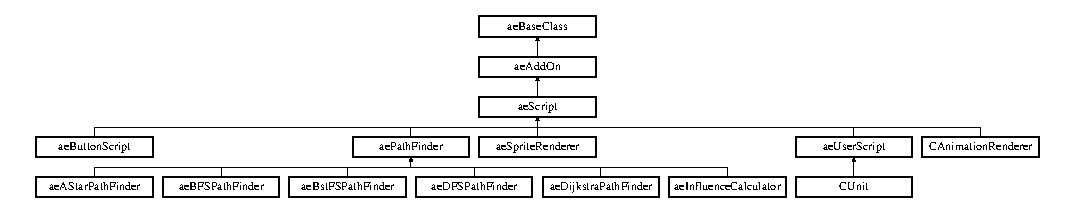
\includegraphics[height=2.430556cm]{classae_add_on}
\end{center}
\end{figure}
\subsection*{Public Member Functions}
\begin{DoxyCompactItemize}
\item 
\hyperlink{_add_on_8h_a10abdd289149f0a510d47930d565b1ea}{Add\+On\+Id} \hyperlink{classae_add_on_a083d2b190df05e023fe65a70514a409f}{Get\+Add\+On\+ID} ()
\begin{DoxyCompactList}\small\item\em Gets add on identifier. \end{DoxyCompactList}\item 
virtual int \hyperlink{classae_add_on_a0730c1446e548031f9a4e98435a54675}{Init} (\hyperlink{classae_base_class}{ae\+Base\+Class} $\ast$p\+Parent)=0
\begin{DoxyCompactList}\small\item\em Initializes with the given parent pointer. \end{DoxyCompactList}\item 
virtual void \hyperlink{classae_add_on_a51caa4b8680206495ea671e71991e231}{Update} (float f\+Delta)=0
\begin{DoxyCompactList}\small\item\em Updates the given f\+Delta. \end{DoxyCompactList}\item 
virtual void \hyperlink{classae_add_on_ab6bed56009b9c92df8ae017a27587dc3}{Render} (ae\+Renderer $\ast$p\+Renderer)
\begin{DoxyCompactList}\small\item\em Paints on the given renderer pointer. \end{DoxyCompactList}\item 
virtual void \hyperlink{classae_add_on_a35cc5d72d19587868c9424603046b331}{Destroy} ()=0\hypertarget{classae_add_on_a35cc5d72d19587868c9424603046b331}{}\label{classae_add_on_a35cc5d72d19587868c9424603046b331}

\begin{DoxyCompactList}\small\item\em Destroys this object. \end{DoxyCompactList}\end{DoxyCompactItemize}
\subsection*{Protected Attributes}
\begin{DoxyCompactItemize}
\item 
\hyperlink{_add_on_8h_a10abdd289149f0a510d47930d565b1ea}{Add\+On\+Id} {\bfseries m\+\_\+n\+Add\+On\+ID}\hypertarget{classae_add_on_acbdd558468d6df44cb95b8581be8d11b}{}\label{classae_add_on_acbdd558468d6df44cb95b8581be8d11b}

\end{DoxyCompactItemize}


\subsection{Detailed Description}
An add on. 

\subsection{Member Function Documentation}
\index{ae\+Add\+On@{ae\+Add\+On}!Get\+Add\+On\+ID@{Get\+Add\+On\+ID}}
\index{Get\+Add\+On\+ID@{Get\+Add\+On\+ID}!ae\+Add\+On@{ae\+Add\+On}}
\subsubsection[{\texorpdfstring{Get\+Add\+On\+I\+D()}{GetAddOnID()}}]{\setlength{\rightskip}{0pt plus 5cm}{\bf Add\+On\+Id} ae\+Add\+On\+::\+Get\+Add\+On\+ID (
\begin{DoxyParamCaption}
{}
\end{DoxyParamCaption}
)}\hypertarget{classae_add_on_a083d2b190df05e023fe65a70514a409f}{}\label{classae_add_on_a083d2b190df05e023fe65a70514a409f}


Gets add on identifier. 

\begin{DoxyReturn}{Returns}
The add on identifier. 
\end{DoxyReturn}
\index{ae\+Add\+On@{ae\+Add\+On}!Init@{Init}}
\index{Init@{Init}!ae\+Add\+On@{ae\+Add\+On}}
\subsubsection[{\texorpdfstring{Init(ae\+Base\+Class $\ast$p\+Parent)=0}{Init(aeBaseClass *pParent)=0}}]{\setlength{\rightskip}{0pt plus 5cm}void ae\+Add\+On\+::\+Init (
\begin{DoxyParamCaption}
\item[{{\bf ae\+Base\+Class} $\ast$}]{p\+Parent}
\end{DoxyParamCaption}
)\hspace{0.3cm}{\ttfamily [pure virtual]}}\hypertarget{classae_add_on_a0730c1446e548031f9a4e98435a54675}{}\label{classae_add_on_a0730c1446e548031f9a4e98435a54675}


Initializes with the given parent pointer. 


\begin{DoxyParams}[1]{Parameters}
\mbox{\tt in,out}  & {\em p\+Parent} & If non-\/null, the parent pointer. \\
\hline
\end{DoxyParams}


Implemented in \hyperlink{classae_a_star_path_finder_ad8de2ad34565b3870ab6ed8c7235cd71}{ae\+A\+Star\+Path\+Finder}, \hyperlink{classae_dijkstra_path_finder_a0cc9454fad1387bba68f879afb1f2526}{ae\+Dijkstra\+Path\+Finder}, \hyperlink{classae_path_finder_a3395375f3de8f3f55d7b780ff6815806}{ae\+Path\+Finder}, \hyperlink{class_c_unit_a092b74e62d924b87deead104dbc08e01}{C\+Unit}, \hyperlink{classae_bst_f_s_path_finder_a83e0028b1394744dc56b703532a88b40}{ae\+Bst\+F\+S\+Path\+Finder}, \hyperlink{classae_b_f_s_path_finder_a23a16f3e98f5c9fc3a6f56a26a7bf170}{ae\+B\+F\+S\+Path\+Finder}, \hyperlink{classae_influence_calculator_ab2607b3e3750770bb23d7e8c4610a49c}{ae\+Influence\+Calculator}, \hyperlink{classae_d_f_s_path_finder_a520c7725e3322b43fd7320da622c1b75}{ae\+D\+F\+S\+Path\+Finder}, \hyperlink{class_c_animation_renderer_abf2ab0201171989cf7ad44846cf3e115}{C\+Animation\+Renderer}, and \hyperlink{classae_sprite_renderer_a97a72a34026e64766a0ab4840376cd76}{ae\+Sprite\+Renderer}.

\index{ae\+Add\+On@{ae\+Add\+On}!Render@{Render}}
\index{Render@{Render}!ae\+Add\+On@{ae\+Add\+On}}
\subsubsection[{\texorpdfstring{Render(ae\+Renderer $\ast$p\+Renderer)}{Render(aeRenderer *pRenderer)}}]{\setlength{\rightskip}{0pt plus 5cm}void ae\+Add\+On\+::\+Render (
\begin{DoxyParamCaption}
\item[{ae\+Renderer $\ast$}]{p\+Renderer}
\end{DoxyParamCaption}
)\hspace{0.3cm}{\ttfamily [inline]}, {\ttfamily [virtual]}}\hypertarget{classae_add_on_ab6bed56009b9c92df8ae017a27587dc3}{}\label{classae_add_on_ab6bed56009b9c92df8ae017a27587dc3}


Paints on the given renderer pointer. 


\begin{DoxyParams}[1]{Parameters}
\mbox{\tt in,out}  & {\em p\+Renderer} & The renderer pointer. \\
\hline
\end{DoxyParams}


Reimplemented in \hyperlink{classae_a_star_path_finder_abfe51663cc9eb452b02b80f335d1c7b0}{ae\+A\+Star\+Path\+Finder}, \hyperlink{classae_dijkstra_path_finder_a75779c09b89c1262cc216f081763927d}{ae\+Dijkstra\+Path\+Finder}, \hyperlink{classae_bst_f_s_path_finder_a6c3646502a67f145cd849392918b4c4b}{ae\+Bst\+F\+S\+Path\+Finder}, \hyperlink{classae_b_f_s_path_finder_a21efc2e873dd066f012ce0ef972a4a85}{ae\+B\+F\+S\+Path\+Finder}, \hyperlink{classae_influence_calculator_a9c48a833f9f81303ec212a9a17d83920}{ae\+Influence\+Calculator}, \hyperlink{classae_d_f_s_path_finder_a2dc1c27f419be5b7a3e94c8be93aede6}{ae\+D\+F\+S\+Path\+Finder}, \hyperlink{class_c_animation_renderer_a272f2bac72c90d89a9ada38058fc3f0c}{C\+Animation\+Renderer}, and \hyperlink{classae_sprite_renderer_a1583eea9478f23549cf9355091542d6a}{ae\+Sprite\+Renderer}.

\index{ae\+Add\+On@{ae\+Add\+On}!Update@{Update}}
\index{Update@{Update}!ae\+Add\+On@{ae\+Add\+On}}
\subsubsection[{\texorpdfstring{Update(float f\+Delta)=0}{Update(float fDelta)=0}}]{\setlength{\rightskip}{0pt plus 5cm}void ae\+Add\+On\+::\+Update (
\begin{DoxyParamCaption}
\item[{float}]{f\+Delta}
\end{DoxyParamCaption}
)\hspace{0.3cm}{\ttfamily [pure virtual]}}\hypertarget{classae_add_on_a51caa4b8680206495ea671e71991e231}{}\label{classae_add_on_a51caa4b8680206495ea671e71991e231}


Updates the given f\+Delta. 


\begin{DoxyParams}{Parameters}
{\em f\+Delta} & The delta time. \\
\hline
\end{DoxyParams}


Implemented in \hyperlink{classae_a_star_path_finder_a21c5d9395cfb810272c89310d037fe15}{ae\+A\+Star\+Path\+Finder}, \hyperlink{classae_dijkstra_path_finder_a400f2f0645f9939bc11c140b3e6cf3d8}{ae\+Dijkstra\+Path\+Finder}, \hyperlink{classae_bst_f_s_path_finder_a27dd4200f183349f605407278de0d086}{ae\+Bst\+F\+S\+Path\+Finder}, \hyperlink{classae_b_f_s_path_finder_a00ddec6c4b37a3df127d1354cbc37635}{ae\+B\+F\+S\+Path\+Finder}, \hyperlink{classae_influence_calculator_af1e3be3558a8e0e0638959ca41734abd}{ae\+Influence\+Calculator}, \hyperlink{classae_d_f_s_path_finder_a7751f27e031719afee45bfd29731b969}{ae\+D\+F\+S\+Path\+Finder}, \hyperlink{class_c_unit_a5f46103027aaf83b2b47c0711640bd69}{C\+Unit}, \hyperlink{class_c_animation_renderer_a2ac2237cb706d2f6d45a88a86543e008}{C\+Animation\+Renderer}, and \hyperlink{classae_sprite_renderer_a65ea9a0ad3452271d2d5b8c140a7eff7}{ae\+Sprite\+Renderer}.



The documentation for this class was generated from the following files\+:\begin{DoxyCompactItemize}
\item 
C\+:/\+Users/\+Alvaro Estrada/\+Documents/\+Visual Studio 2015/\+Projects/\+R\+T\+S\+\_\+\+A\+E/\+R\+T\+S\+\_\+\+A\+E/\+Game/\hyperlink{_add_on_8h}{Add\+On.\+h}\item 
C\+:/\+Users/\+Alvaro Estrada/\+Documents/\+Visual Studio 2015/\+Projects/\+R\+T\+S\+\_\+\+A\+E/\+R\+T\+S\+\_\+\+A\+E/\+Game/Add\+On.\+cpp\end{DoxyCompactItemize}

\hypertarget{classae_app}{}\section{ae\+App Class Reference}
\label{classae_app}\index{ae\+App@{ae\+App}}
\subsection*{Public Member Functions}
\begin{DoxyCompactItemize}
\item 
int {\bfseries Init} ()\hypertarget{classae_app_a1ec791a1492ce55fddcbac02646652c8}{}\label{classae_app_a1ec791a1492ce55fddcbac02646652c8}

\item 
bool {\bfseries Is\+Running} ()\hypertarget{classae_app_a688edeae06699cf509997caa7700888b}{}\label{classae_app_a688edeae06699cf509997caa7700888b}

\item 
void {\bfseries Update} ()\hypertarget{classae_app_a7a822d98e9d2aa6bfe116c48089cc4f5}{}\label{classae_app_a7a822d98e9d2aa6bfe116c48089cc4f5}

\item 
void {\bfseries Destroy} ()\hypertarget{classae_app_a4474aff034a1d4dfe0e52bb5e2e6e052}{}\label{classae_app_a4474aff034a1d4dfe0e52bb5e2e6e052}

\end{DoxyCompactItemize}
\subsection*{Static Public Member Functions}
\begin{DoxyCompactItemize}
\item 
static \hyperlink{namespaceae_core_ad6f85aacc0d1fdd85e458e2413e60010}{ae\+String} {\bfseries Get\+File\+Path} ()\hypertarget{classae_app_acd34035805bbad3884140adc0aba8ab1}{}\label{classae_app_acd34035805bbad3884140adc0aba8ab1}

\item 
static int {\bfseries App\+Load\+Variables} (void $\ast$data, int argument\+\_\+count, char $\ast$$\ast$argument\+\_\+values, char $\ast$$\ast$psz\+Col\+Name)\hypertarget{classae_app_a3f46560d28b0fdebd3896458f78fccb0}{}\label{classae_app_a3f46560d28b0fdebd3896458f78fccb0}

\item 
static int {\bfseries Window\+Load\+Variables} (void $\ast$data, int argument\+\_\+count, char $\ast$$\ast$argument\+\_\+values, char $\ast$$\ast$psz\+Col\+Name)\hypertarget{classae_app_a61ef0f02f1c9777b88cb58ef805bab67}{}\label{classae_app_a61ef0f02f1c9777b88cb58ef805bab67}

\item 
static int {\bfseries G\+U\+I\+Load\+Variables} (void $\ast$data, int argument\+\_\+count, char $\ast$$\ast$argument\+\_\+values, char $\ast$$\ast$psz\+Col\+Name)\hypertarget{classae_app_add558af8ee1566519662804c6cc55d33}{}\label{classae_app_add558af8ee1566519662804c6cc55d33}

\item 
static int {\bfseries Timer\+Load\+Variables} (void $\ast$data, int argument\+\_\+count, char $\ast$$\ast$argument\+\_\+values, char $\ast$$\ast$psz\+Col\+Name)\hypertarget{classae_app_a516d0ec1b931513a9949c4d71a47c81d}{}\label{classae_app_a516d0ec1b931513a9949c4d71a47c81d}

\item 
static int {\bfseries Sprites\+Creation} (void $\ast$data, int argument\+\_\+count, char $\ast$$\ast$argument\+\_\+values, char $\ast$$\ast$psz\+Col\+Name)\hypertarget{classae_app_a506664678993d20e64015645a5fd0c9f}{}\label{classae_app_a506664678993d20e64015645a5fd0c9f}

\end{DoxyCompactItemize}


The documentation for this class was generated from the following files\+:\begin{DoxyCompactItemize}
\item 
C\+:/\+Users/\+Alvaro Estrada/\+Documents/\+Visual Studio 2015/\+Projects/\+R\+T\+S\+\_\+\+A\+E/\+R\+T\+S\+\_\+\+A\+E/\+Game/App.\+h\item 
C\+:/\+Users/\+Alvaro Estrada/\+Documents/\+Visual Studio 2015/\+Projects/\+R\+T\+S\+\_\+\+A\+E/\+R\+T\+S\+\_\+\+A\+E/\+Game/App.\+cpp\end{DoxyCompactItemize}

\hypertarget{classae_core_1_1ae_app_window}{}\section{ae\+Core\+:\+:ae\+App\+Window Class Reference}
\label{classae_core_1_1ae_app_window}\index{ae\+Core\+::ae\+App\+Window@{ae\+Core\+::ae\+App\+Window}}


This class purpose is to create a client window where the entire program will display.  




{\ttfamily \#include $<$App\+Window.\+h$>$}

\subsection*{Classes}
\begin{DoxyCompactItemize}
\item 
struct \hyperlink{structae_core_1_1ae_app_window_1_1_on_load}{On\+Load}
\end{DoxyCompactItemize}
\subsection*{Public Member Functions}
\begin{DoxyCompactItemize}
\item 
\hyperlink{classae_core_1_1ae_app_window_a6564607e8220037c8c2e716be8b99434}{ae\+App\+Window} ()\hypertarget{classae_core_1_1ae_app_window_a6564607e8220037c8c2e716be8b99434}{}\label{classae_core_1_1ae_app_window_a6564607e8220037c8c2e716be8b99434}

\begin{DoxyCompactList}\small\item\em Default constructor. \end{DoxyCompactList}\item 
\hyperlink{classae_core_1_1ae_app_window_a61315b1f493416e3a5d2d10fa9b20e76}{$\sim$ae\+App\+Window} ()\hypertarget{classae_core_1_1ae_app_window_a61315b1f493416e3a5d2d10fa9b20e76}{}\label{classae_core_1_1ae_app_window_a61315b1f493416e3a5d2d10fa9b20e76}

\begin{DoxyCompactList}\small\item\em Destructor. \end{DoxyCompactList}\item 
int \hyperlink{classae_core_1_1ae_app_window_a9dc8d3c42a0f4983b5158939f4156f00}{Init} (\hyperlink{structae_core_1_1ae_app_window_1_1_on_load}{On\+Load} \&On\+Load\+Variables, \hyperlink{classae_core_1_1ae_renderer}{ae\+Renderer} $\ast$p\+Renderer)
\begin{DoxyCompactList}\small\item\em Starts S\+DL and creates a window. Gets 0 if it was initialized correctly, otherwise, it will get an error number. \end{DoxyCompactList}\item 
void \hyperlink{classae_core_1_1ae_app_window_af1380617f379039d9d3165af34e2e15c}{Render} (\hyperlink{classae_core_1_1ae_renderer}{ae\+Renderer} $\ast$p\+Renderer)
\begin{DoxyCompactList}\small\item\em Renders this object. \end{DoxyCompactList}\item 
void \hyperlink{classae_core_1_1ae_app_window_ad015b4cd20e3b933ef452bbbacb19883}{Destroy} ()
\begin{DoxyCompactList}\small\item\em Destroys the Window. \end{DoxyCompactList}\item 
int \hyperlink{classae_core_1_1ae_app_window_a605ca0eaea8e88da799e2e7ab9ea6ac4}{Get\+Width} ()
\begin{DoxyCompactList}\small\item\em Gets the width. \end{DoxyCompactList}\item 
int \hyperlink{classae_core_1_1ae_app_window_ad866314100400fcd0c2b55f4cd1593b0}{Get\+Height} ()
\begin{DoxyCompactList}\small\item\em Gets the height. \end{DoxyCompactList}\item 
int \hyperlink{classae_core_1_1ae_app_window_a09c1975c182c6e764d0a28514780e18f}{Get\+PosX} ()
\begin{DoxyCompactList}\small\item\em Gets position x coordinate. \end{DoxyCompactList}\item 
int \hyperlink{classae_core_1_1ae_app_window_a472c4aa17271b0a81dede5110227c324}{Get\+PosY} ()
\begin{DoxyCompactList}\small\item\em Gets position y coordinate. \end{DoxyCompactList}\item 
void \hyperlink{classae_core_1_1ae_app_window_affdc864ae469c97a4b442485b423b4c5}{Process\+Window\+Events} ()\hypertarget{classae_core_1_1ae_app_window_affdc864ae469c97a4b442485b423b4c5}{}\label{classae_core_1_1ae_app_window_affdc864ae469c97a4b442485b423b4c5}

\begin{DoxyCompactList}\small\item\em Process the events generated by the window. \end{DoxyCompactList}\end{DoxyCompactItemize}
\subsection*{Protected Member Functions}
\begin{DoxyCompactItemize}
\item 
int \hyperlink{classae_core_1_1ae_app_window_a6be4903a3ccd59a7cf13273713c97ee6}{Get\+Num\+Of\+Driver} (char $\ast$psz\+Driver\+Name)
\begin{DoxyCompactList}\small\item\em Gets number of the given driver name. If the driver is not found, returns -\/1;. \end{DoxyCompactList}\end{DoxyCompactItemize}
\subsection*{Protected Attributes}
\begin{DoxyCompactItemize}
\item 
S\+D\+L\+\_\+\+Window $\ast$ {\bfseries m\+\_\+p\+S\+D\+L\+Window}\hypertarget{classae_core_1_1ae_app_window_a623a750256b968ba0d166b80ab278dfb}{}\label{classae_core_1_1ae_app_window_a623a750256b968ba0d166b80ab278dfb}

\item 
S\+D\+L\+\_\+\+Event {\bfseries m\+\_\+\+Event\+Manager}\hypertarget{classae_core_1_1ae_app_window_a8488cd70bd33a42e4d1aedc8c52406cc}{}\label{classae_core_1_1ae_app_window_a8488cd70bd33a42e4d1aedc8c52406cc}

\item 
int {\bfseries m\+\_\+nX}\hypertarget{classae_core_1_1ae_app_window_aaa518091b236dc363d85d730a5997bd1}{}\label{classae_core_1_1ae_app_window_aaa518091b236dc363d85d730a5997bd1}

\item 
int {\bfseries m\+\_\+nY}\hypertarget{classae_core_1_1ae_app_window_a4af3e59640e73609ca1f0e360a23660a}{}\label{classae_core_1_1ae_app_window_a4af3e59640e73609ca1f0e360a23660a}

\item 
int {\bfseries m\+\_\+n\+Width}\hypertarget{classae_core_1_1ae_app_window_add39b144d8a4ee68140b584255bb2d90}{}\label{classae_core_1_1ae_app_window_add39b144d8a4ee68140b584255bb2d90}

\item 
int {\bfseries m\+\_\+n\+Height}\hypertarget{classae_core_1_1ae_app_window_a0261e767dab03b2dfe8ffeaffe6c3ba0}{}\label{classae_core_1_1ae_app_window_a0261e767dab03b2dfe8ffeaffe6c3ba0}

\end{DoxyCompactItemize}


\subsection{Detailed Description}
This class purpose is to create a client window where the entire program will display. 

\subsection{Member Function Documentation}
\index{ae\+Core\+::ae\+App\+Window@{ae\+Core\+::ae\+App\+Window}!Destroy@{Destroy}}
\index{Destroy@{Destroy}!ae\+Core\+::ae\+App\+Window@{ae\+Core\+::ae\+App\+Window}}
\subsubsection[{\texorpdfstring{Destroy()}{Destroy()}}]{\setlength{\rightskip}{0pt plus 5cm}void ae\+Core\+::ae\+App\+Window\+::\+Destroy (
\begin{DoxyParamCaption}
{}
\end{DoxyParamCaption}
)}\hypertarget{classae_core_1_1ae_app_window_ad015b4cd20e3b933ef452bbbacb19883}{}\label{classae_core_1_1ae_app_window_ad015b4cd20e3b933ef452bbbacb19883}


Destroys the Window. 

Closes the S\+DL window and cleans up the source. \index{ae\+Core\+::ae\+App\+Window@{ae\+Core\+::ae\+App\+Window}!Get\+Height@{Get\+Height}}
\index{Get\+Height@{Get\+Height}!ae\+Core\+::ae\+App\+Window@{ae\+Core\+::ae\+App\+Window}}
\subsubsection[{\texorpdfstring{Get\+Height()}{GetHeight()}}]{\setlength{\rightskip}{0pt plus 5cm}int ae\+Core\+::ae\+App\+Window\+::\+Get\+Height (
\begin{DoxyParamCaption}
{}
\end{DoxyParamCaption}
)}\hypertarget{classae_core_1_1ae_app_window_ad866314100400fcd0c2b55f4cd1593b0}{}\label{classae_core_1_1ae_app_window_ad866314100400fcd0c2b55f4cd1593b0}


Gets the height. 

\begin{DoxyReturn}{Returns}
The height. 
\end{DoxyReturn}
\index{ae\+Core\+::ae\+App\+Window@{ae\+Core\+::ae\+App\+Window}!Get\+Num\+Of\+Driver@{Get\+Num\+Of\+Driver}}
\index{Get\+Num\+Of\+Driver@{Get\+Num\+Of\+Driver}!ae\+Core\+::ae\+App\+Window@{ae\+Core\+::ae\+App\+Window}}
\subsubsection[{\texorpdfstring{Get\+Num\+Of\+Driver(char $\ast$psz\+Driver\+Name)}{GetNumOfDriver(char *pszDriverName)}}]{\setlength{\rightskip}{0pt plus 5cm}int ae\+Core\+::ae\+App\+Window\+::\+Get\+Num\+Of\+Driver (
\begin{DoxyParamCaption}
\item[{char $\ast$}]{psz\+Driver\+Name}
\end{DoxyParamCaption}
)\hspace{0.3cm}{\ttfamily [protected]}}\hypertarget{classae_core_1_1ae_app_window_a6be4903a3ccd59a7cf13273713c97ee6}{}\label{classae_core_1_1ae_app_window_a6be4903a3ccd59a7cf13273713c97ee6}


Gets number of the given driver name. If the driver is not found, returns -\/1;. 


\begin{DoxyParams}[1]{Parameters}
\mbox{\tt in,out}  & {\em psz\+Driver\+Name} & If non-\/null, name of the driver.\\
\hline
\end{DoxyParams}
\begin{DoxyReturn}{Returns}
The number of driver. 
\end{DoxyReturn}
\index{ae\+Core\+::ae\+App\+Window@{ae\+Core\+::ae\+App\+Window}!Get\+PosX@{Get\+PosX}}
\index{Get\+PosX@{Get\+PosX}!ae\+Core\+::ae\+App\+Window@{ae\+Core\+::ae\+App\+Window}}
\subsubsection[{\texorpdfstring{Get\+Pos\+X()}{GetPosX()}}]{\setlength{\rightskip}{0pt plus 5cm}int ae\+Core\+::ae\+App\+Window\+::\+Get\+PosX (
\begin{DoxyParamCaption}
{}
\end{DoxyParamCaption}
)}\hypertarget{classae_core_1_1ae_app_window_a09c1975c182c6e764d0a28514780e18f}{}\label{classae_core_1_1ae_app_window_a09c1975c182c6e764d0a28514780e18f}


Gets position x coordinate. 

\begin{DoxyReturn}{Returns}
The position x coordinate. 
\end{DoxyReturn}
\index{ae\+Core\+::ae\+App\+Window@{ae\+Core\+::ae\+App\+Window}!Get\+PosY@{Get\+PosY}}
\index{Get\+PosY@{Get\+PosY}!ae\+Core\+::ae\+App\+Window@{ae\+Core\+::ae\+App\+Window}}
\subsubsection[{\texorpdfstring{Get\+Pos\+Y()}{GetPosY()}}]{\setlength{\rightskip}{0pt plus 5cm}int ae\+Core\+::ae\+App\+Window\+::\+Get\+PosY (
\begin{DoxyParamCaption}
{}
\end{DoxyParamCaption}
)}\hypertarget{classae_core_1_1ae_app_window_a472c4aa17271b0a81dede5110227c324}{}\label{classae_core_1_1ae_app_window_a472c4aa17271b0a81dede5110227c324}


Gets position y coordinate. 

\begin{DoxyReturn}{Returns}
The position y coordinate. 
\end{DoxyReturn}
\index{ae\+Core\+::ae\+App\+Window@{ae\+Core\+::ae\+App\+Window}!Get\+Width@{Get\+Width}}
\index{Get\+Width@{Get\+Width}!ae\+Core\+::ae\+App\+Window@{ae\+Core\+::ae\+App\+Window}}
\subsubsection[{\texorpdfstring{Get\+Width()}{GetWidth()}}]{\setlength{\rightskip}{0pt plus 5cm}int ae\+Core\+::ae\+App\+Window\+::\+Get\+Width (
\begin{DoxyParamCaption}
{}
\end{DoxyParamCaption}
)}\hypertarget{classae_core_1_1ae_app_window_a605ca0eaea8e88da799e2e7ab9ea6ac4}{}\label{classae_core_1_1ae_app_window_a605ca0eaea8e88da799e2e7ab9ea6ac4}


Gets the width. 

\begin{DoxyReturn}{Returns}
The width. 
\end{DoxyReturn}
\index{ae\+Core\+::ae\+App\+Window@{ae\+Core\+::ae\+App\+Window}!Init@{Init}}
\index{Init@{Init}!ae\+Core\+::ae\+App\+Window@{ae\+Core\+::ae\+App\+Window}}
\subsubsection[{\texorpdfstring{Init(\+On\+Load \&\+On\+Load\+Variables, ae\+Renderer $\ast$p\+Renderer)}{Init(OnLoad &OnLoadVariables, aeRenderer *pRenderer)}}]{\setlength{\rightskip}{0pt plus 5cm}int ae\+Core\+::ae\+App\+Window\+::\+Init (
\begin{DoxyParamCaption}
\item[{{\bf On\+Load} \&}]{On\+Load\+Variables, }
\item[{{\bf ae\+Renderer} $\ast$}]{p\+Renderer}
\end{DoxyParamCaption}
)}\hypertarget{classae_core_1_1ae_app_window_a9dc8d3c42a0f4983b5158939f4156f00}{}\label{classae_core_1_1ae_app_window_a9dc8d3c42a0f4983b5158939f4156f00}


Starts S\+DL and creates a window. Gets 0 if it was initialized correctly, otherwise, it will get an error number. 


\begin{DoxyParams}[1]{Parameters}
\mbox{\tt in,out}  & {\em On\+Load\+Variables} & The on load variables. \\
\hline
\mbox{\tt in,out}  & {\em p\+Renderer} & If non-\/null, the renderer.\\
\hline
\end{DoxyParams}
\begin{DoxyReturn}{Returns}
An int. 
\end{DoxyReturn}
\index{ae\+Core\+::ae\+App\+Window@{ae\+Core\+::ae\+App\+Window}!Render@{Render}}
\index{Render@{Render}!ae\+Core\+::ae\+App\+Window@{ae\+Core\+::ae\+App\+Window}}
\subsubsection[{\texorpdfstring{Render(ae\+Renderer $\ast$p\+Renderer)}{Render(aeRenderer *pRenderer)}}]{\setlength{\rightskip}{0pt plus 5cm}void ae\+Core\+::ae\+App\+Window\+::\+Render (
\begin{DoxyParamCaption}
\item[{{\bf ae\+Renderer} $\ast$}]{p\+Renderer}
\end{DoxyParamCaption}
)}\hypertarget{classae_core_1_1ae_app_window_af1380617f379039d9d3165af34e2e15c}{}\label{classae_core_1_1ae_app_window_af1380617f379039d9d3165af34e2e15c}


Renders this object. 

Renders the given renderer pointer.


\begin{DoxyParams}[1]{Parameters}
\mbox{\tt in,out}  & {\em p\+Renderer} & If non-\/null, the renderer. \\
\hline
\end{DoxyParams}


The documentation for this class was generated from the following files\+:\begin{DoxyCompactItemize}
\item 
C\+:/\+Users/\+Alvaro Estrada/\+Documents/\+Visual Studio 2015/\+Projects/\+R\+T\+S\+\_\+\+A\+E/ae\+Core/\+Graphics/\hyperlink{_app_window_8h}{App\+Window.\+h}\item 
C\+:/\+Users/\+Alvaro Estrada/\+Documents/\+Visual Studio 2015/\+Projects/\+R\+T\+S\+\_\+\+A\+E/ae\+Core/\+Graphics/\hyperlink{_app_window_8cpp}{App\+Window.\+cpp}\end{DoxyCompactItemize}

\hypertarget{classae_a_star_map_tile_node}{}\section{ae\+A\+Star\+Map\+Tile\+Node Class Reference}
\label{classae_a_star_map_tile_node}\index{ae\+A\+Star\+Map\+Tile\+Node@{ae\+A\+Star\+Map\+Tile\+Node}}
Inheritance diagram for ae\+A\+Star\+Map\+Tile\+Node\+:\begin{figure}[H]
\begin{center}
\leavevmode
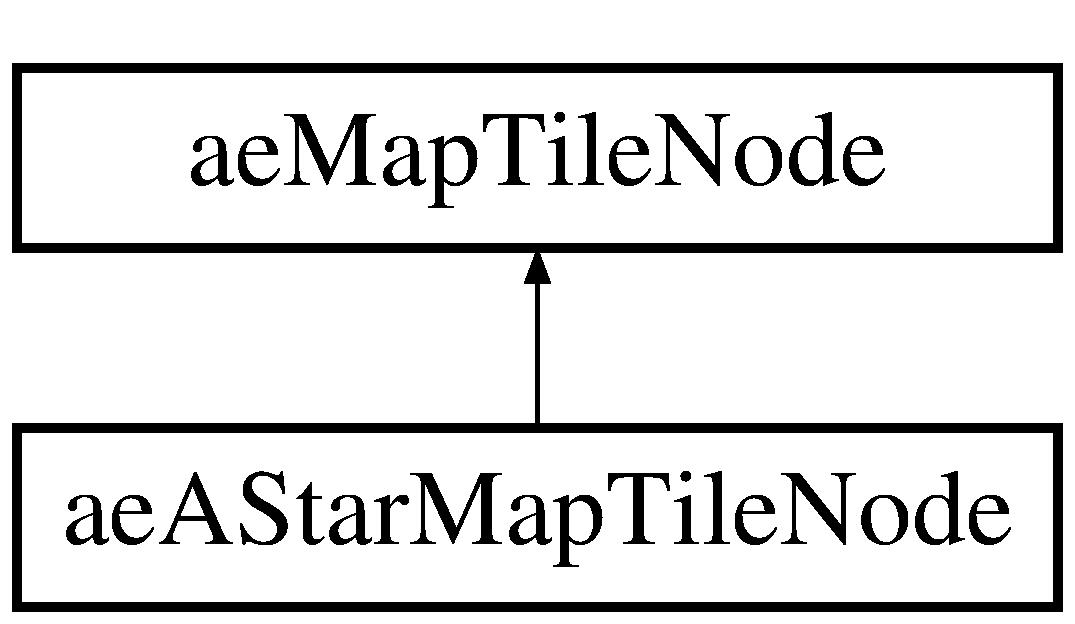
\includegraphics[height=2.000000cm]{classae_a_star_map_tile_node}
\end{center}
\end{figure}
\subsection*{Public Member Functions}
\begin{DoxyCompactItemize}
\item 
{\bfseries ae\+A\+Star\+Map\+Tile\+Node} (const \hyperlink{classae_a_star_map_tile_node}{ae\+A\+Star\+Map\+Tile\+Node} \&copy)\hypertarget{classae_a_star_map_tile_node_a3a28c8095b51996f6f1774c14699c81d}{}\label{classae_a_star_map_tile_node_a3a28c8095b51996f6f1774c14699c81d}

\item 
virtual \hyperlink{classae_a_star_map_tile_node}{ae\+A\+Star\+Map\+Tile\+Node} \& {\bfseries operator=} (const \hyperlink{classae_a_star_map_tile_node}{ae\+A\+Star\+Map\+Tile\+Node} \&rhs)\hypertarget{classae_a_star_map_tile_node_ac113dd7d8732e2030012f3cfd71302ed}{}\label{classae_a_star_map_tile_node_ac113dd7d8732e2030012f3cfd71302ed}

\item 
virtual void {\bfseries Set\+Cost} (const \hyperlink{namespaceae_core_a862bc39eb87cfabca273f49e2a920129}{int32} cost)\hypertarget{classae_a_star_map_tile_node_ad12ae4cc9a10248ac05cd3c4414048d4}{}\label{classae_a_star_map_tile_node_ad12ae4cc9a10248ac05cd3c4414048d4}

\item 
virtual \hyperlink{namespaceae_core_a862bc39eb87cfabca273f49e2a920129}{int32} {\bfseries Get\+Cost} () const \hypertarget{classae_a_star_map_tile_node_a0cdbab3cfca6974bade79bf11d2297f4}{}\label{classae_a_star_map_tile_node_a0cdbab3cfca6974bade79bf11d2297f4}

\end{DoxyCompactItemize}
\subsection*{Public Attributes}
\begin{DoxyCompactItemize}
\item 
int32 {\bfseries m\+\_\+f}\hypertarget{classae_a_star_map_tile_node_a6aa180e132d3fae48cb15114dcbda6b5}{}\label{classae_a_star_map_tile_node_a6aa180e132d3fae48cb15114dcbda6b5}

\item 
int32 {\bfseries m\+\_\+g}\hypertarget{classae_a_star_map_tile_node_ada96741068c42e62e0ab145218806eab}{}\label{classae_a_star_map_tile_node_ada96741068c42e62e0ab145218806eab}

\item 
int32 {\bfseries m\+\_\+h}\hypertarget{classae_a_star_map_tile_node_a7af7a86c9c8bea92fdc515d78bdac447}{}\label{classae_a_star_map_tile_node_a7af7a86c9c8bea92fdc515d78bdac447}

\end{DoxyCompactItemize}


The documentation for this class was generated from the following files\+:\begin{DoxyCompactItemize}
\item 
C\+:/\+Users/\+Alvaro Estrada/\+Documents/\+Visual Studio 2015/\+Projects/\+R\+T\+S\+\_\+\+A\+E/\+R\+T\+S\+\_\+\+A\+E/\+Game/\hyperlink{_map_tile_node_8h}{Map\+Tile\+Node.\+h}\item 
C\+:/\+Users/\+Alvaro Estrada/\+Documents/\+Visual Studio 2015/\+Projects/\+R\+T\+S\+\_\+\+A\+E/\+R\+T\+S\+\_\+\+A\+E/\+Game/\hyperlink{_map_tile_node_8cpp}{Map\+Tile\+Node.\+cpp}\end{DoxyCompactItemize}

\hypertarget{classae_a_star_path_finder}{}\section{ae\+A\+Star\+Path\+Finder Class Reference}
\label{classae_a_star_path_finder}\index{ae\+A\+Star\+Path\+Finder@{ae\+A\+Star\+Path\+Finder}}
Inheritance diagram for ae\+A\+Star\+Path\+Finder\+:\begin{figure}[H]
\begin{center}
\leavevmode
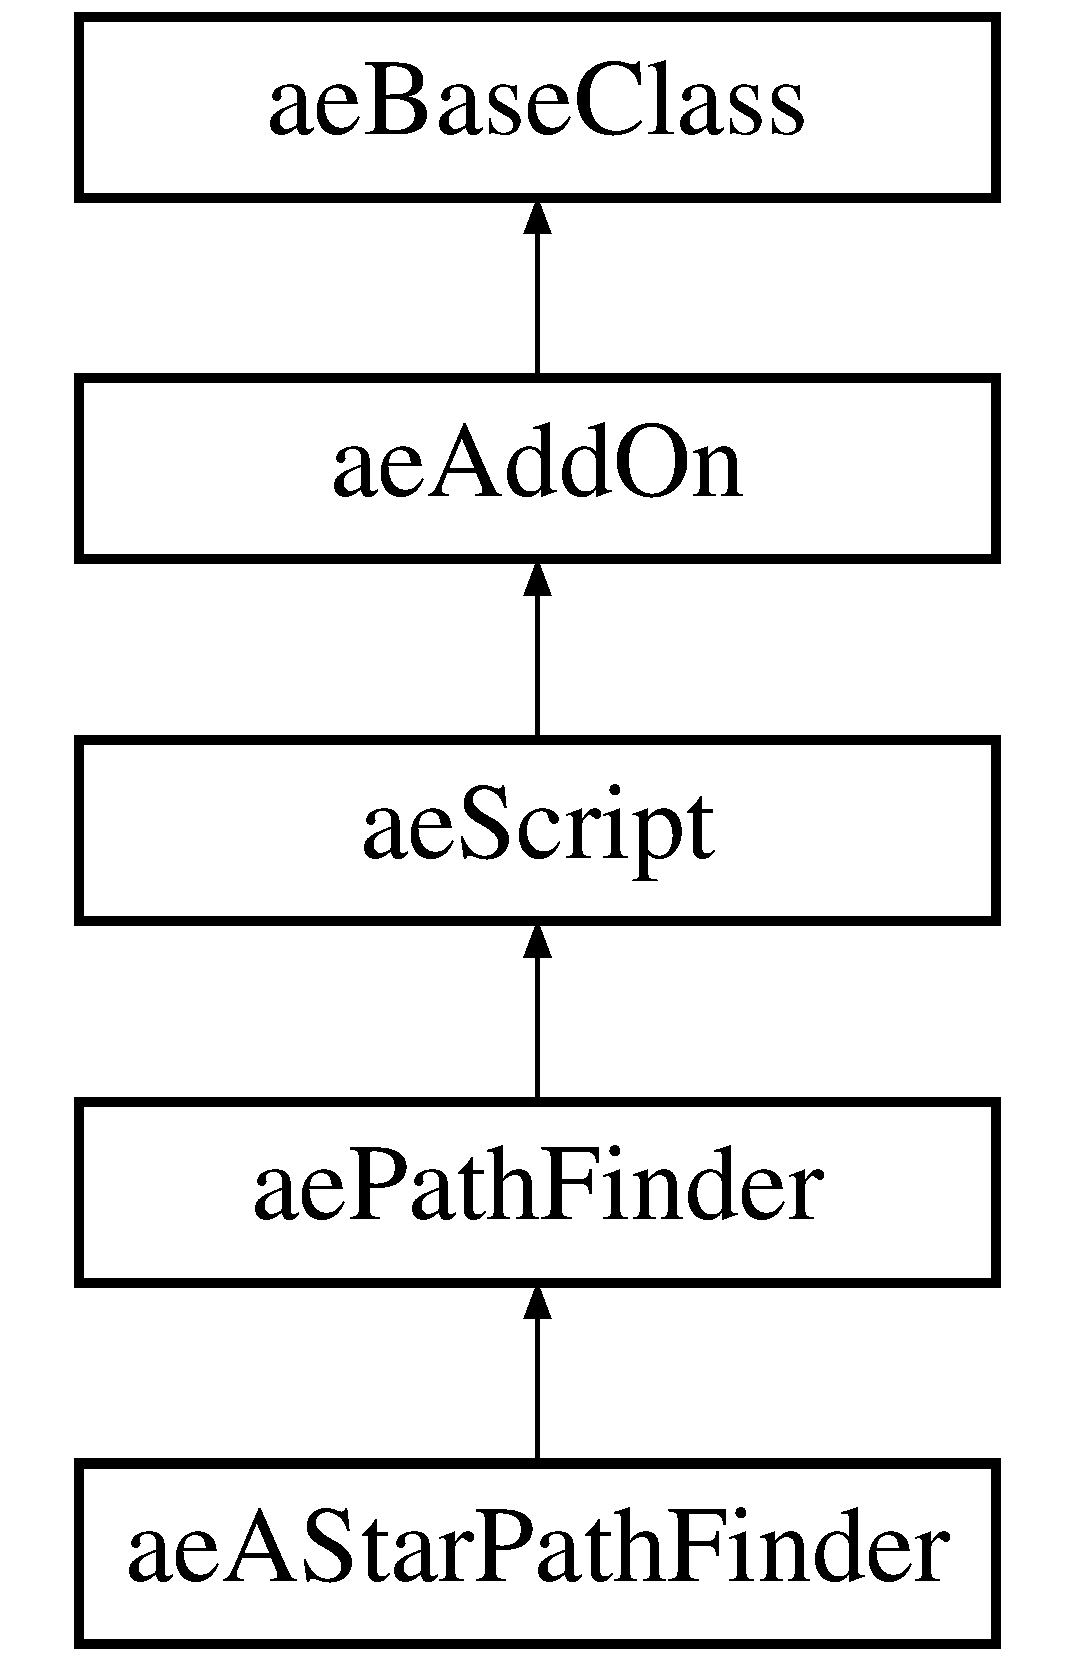
\includegraphics[height=5.000000cm]{classae_a_star_path_finder}
\end{center}
\end{figure}
\subsection*{Classes}
\begin{DoxyCompactItemize}
\item 
struct \hyperlink{structae_a_star_path_finder_1_1_node_dist}{Node\+Dist}
\item 
struct \hyperlink{structae_a_star_path_finder_1_1_tile_compare}{Tile\+Compare}
\end{DoxyCompactItemize}
\subsection*{Public Member Functions}
\begin{DoxyCompactItemize}
\item 
{\bfseries ae\+A\+Star\+Path\+Finder} (\hyperlink{classae_tiled_map}{ae\+Tiled\+Map} $\ast$p\+Map)\hypertarget{classae_a_star_path_finder_ab91a80de31e37c0fb9a062b800e12568}{}\label{classae_a_star_path_finder_ab91a80de31e37c0fb9a062b800e12568}

\item 
virtual int \hyperlink{classae_a_star_path_finder_ad8de2ad34565b3870ab6ed8c7235cd71}{Init} (\hyperlink{classae_base_class}{ae\+Base\+Class} $\ast$p\+Parent)
\begin{DoxyCompactList}\small\item\em Initializes with the given parent pointer. \end{DoxyCompactList}\item 
virtual void \hyperlink{classae_a_star_path_finder_a54e53b0396e46112c69b03a34eaf3900}{Destroy} ()\hypertarget{classae_a_star_path_finder_a54e53b0396e46112c69b03a34eaf3900}{}\label{classae_a_star_path_finder_a54e53b0396e46112c69b03a34eaf3900}

\begin{DoxyCompactList}\small\item\em Destroys this object. \end{DoxyCompactList}\item 
virtual void \hyperlink{classae_a_star_path_finder_a21c5d9395cfb810272c89310d037fe15}{Update} (float f\+Delta)
\begin{DoxyCompactList}\small\item\em Updates the given f\+Delta. \end{DoxyCompactList}\item 
virtual void \hyperlink{classae_a_star_path_finder_abfe51663cc9eb452b02b80f335d1c7b0}{Render} (\hyperlink{classae_core_1_1ae_renderer}{ae\+Renderer} $\ast$p\+Renderer)
\begin{DoxyCompactList}\small\item\em Renders the given Renderer pointer. \end{DoxyCompactList}\item 
virtual void \hyperlink{classae_a_star_path_finder_a863caf99db47beef104b3315dde43a45}{Reset} ()\hypertarget{classae_a_star_path_finder_a863caf99db47beef104b3315dde43a45}{}\label{classae_a_star_path_finder_a863caf99db47beef104b3315dde43a45}

\begin{DoxyCompactList}\small\item\em Resets this object. \end{DoxyCompactList}\end{DoxyCompactItemize}
\subsection*{Protected Member Functions}
\begin{DoxyCompactItemize}
\item 
virtual void \hyperlink{classae_a_star_path_finder_a3263c66da32aea8e2f6567754110c63c}{Visit\+Grid\+Node} (\hyperlink{namespaceae_core_a862bc39eb87cfabca273f49e2a920129}{int32} x, \hyperlink{namespaceae_core_a862bc39eb87cfabca273f49e2a920129}{int32} y)
\begin{DoxyCompactList}\small\item\em Marks a node as visited. \end{DoxyCompactList}\item 
virtual Walk\+State\+ID \hyperlink{classae_a_star_path_finder_a3a23dcf11eccaf75a71179c602ebb1b0}{Give\+A\+Step} ()
\begin{DoxyCompactList}\small\item\em Give a step. \end{DoxyCompactList}\end{DoxyCompactItemize}
\subsection*{Additional Inherited Members}


\subsection{Member Function Documentation}
\index{ae\+A\+Star\+Path\+Finder@{ae\+A\+Star\+Path\+Finder}!Give\+A\+Step@{Give\+A\+Step}}
\index{Give\+A\+Step@{Give\+A\+Step}!ae\+A\+Star\+Path\+Finder@{ae\+A\+Star\+Path\+Finder}}
\subsubsection[{\texorpdfstring{Give\+A\+Step()}{GiveAStep()}}]{\setlength{\rightskip}{0pt plus 5cm}Walk\+State\+ID ae\+A\+Star\+Path\+Finder\+::\+Give\+A\+Step (
\begin{DoxyParamCaption}
{}
\end{DoxyParamCaption}
)\hspace{0.3cm}{\ttfamily [protected]}, {\ttfamily [virtual]}}\hypertarget{classae_a_star_path_finder_a3a23dcf11eccaf75a71179c602ebb1b0}{}\label{classae_a_star_path_finder_a3a23dcf11eccaf75a71179c602ebb1b0}


Give a step. 

\begin{DoxyReturn}{Returns}
A Walk\+State\+ID. 
\end{DoxyReturn}


Implements \hyperlink{classae_path_finder_a49332ee3be744cac1ece9ffd503ca218}{ae\+Path\+Finder}.

\index{ae\+A\+Star\+Path\+Finder@{ae\+A\+Star\+Path\+Finder}!Init@{Init}}
\index{Init@{Init}!ae\+A\+Star\+Path\+Finder@{ae\+A\+Star\+Path\+Finder}}
\subsubsection[{\texorpdfstring{Init(ae\+Base\+Class $\ast$p\+Parent)}{Init(aeBaseClass *pParent)}}]{\setlength{\rightskip}{0pt plus 5cm}int ae\+A\+Star\+Path\+Finder\+::\+Init (
\begin{DoxyParamCaption}
\item[{{\bf ae\+Base\+Class} $\ast$}]{p\+Parent}
\end{DoxyParamCaption}
)\hspace{0.3cm}{\ttfamily [virtual]}}\hypertarget{classae_a_star_path_finder_ad8de2ad34565b3870ab6ed8c7235cd71}{}\label{classae_a_star_path_finder_ad8de2ad34565b3870ab6ed8c7235cd71}


Initializes with the given parent pointer. 


\begin{DoxyParams}[1]{Parameters}
\mbox{\tt in,out}  & {\em p\+Parent} & If non-\/null, the parent.\\
\hline
\end{DoxyParams}
\begin{DoxyReturn}{Returns}
An int. 
\end{DoxyReturn}


Reimplemented from \hyperlink{classae_path_finder_a3395375f3de8f3f55d7b780ff6815806}{ae\+Path\+Finder}.

\index{ae\+A\+Star\+Path\+Finder@{ae\+A\+Star\+Path\+Finder}!Render@{Render}}
\index{Render@{Render}!ae\+A\+Star\+Path\+Finder@{ae\+A\+Star\+Path\+Finder}}
\subsubsection[{\texorpdfstring{Render(ae\+Renderer $\ast$p\+Renderer)}{Render(aeRenderer *pRenderer)}}]{\setlength{\rightskip}{0pt plus 5cm}void ae\+A\+Star\+Path\+Finder\+::\+Render (
\begin{DoxyParamCaption}
\item[{{\bf ae\+Renderer} $\ast$}]{p\+Renderer}
\end{DoxyParamCaption}
)\hspace{0.3cm}{\ttfamily [virtual]}}\hypertarget{classae_a_star_path_finder_abfe51663cc9eb452b02b80f335d1c7b0}{}\label{classae_a_star_path_finder_abfe51663cc9eb452b02b80f335d1c7b0}


Renders the given Renderer pointer. 


\begin{DoxyParams}[1]{Parameters}
\mbox{\tt in,out}  & {\em p\+Renderer} & If non-\/null, the renderer. \\
\hline
\end{DoxyParams}


Reimplemented from \hyperlink{classae_add_on_ab6bed56009b9c92df8ae017a27587dc3}{ae\+Add\+On}.

\index{ae\+A\+Star\+Path\+Finder@{ae\+A\+Star\+Path\+Finder}!Update@{Update}}
\index{Update@{Update}!ae\+A\+Star\+Path\+Finder@{ae\+A\+Star\+Path\+Finder}}
\subsubsection[{\texorpdfstring{Update(float f\+Delta)}{Update(float fDelta)}}]{\setlength{\rightskip}{0pt plus 5cm}void ae\+A\+Star\+Path\+Finder\+::\+Update (
\begin{DoxyParamCaption}
\item[{float}]{f\+Delta}
\end{DoxyParamCaption}
)\hspace{0.3cm}{\ttfamily [virtual]}}\hypertarget{classae_a_star_path_finder_a21c5d9395cfb810272c89310d037fe15}{}\label{classae_a_star_path_finder_a21c5d9395cfb810272c89310d037fe15}


Updates the given f\+Delta. 


\begin{DoxyParams}{Parameters}
{\em f\+Delta} & The delta. \\
\hline
\end{DoxyParams}


Implements \hyperlink{classae_add_on_a51caa4b8680206495ea671e71991e231}{ae\+Add\+On}.

\index{ae\+A\+Star\+Path\+Finder@{ae\+A\+Star\+Path\+Finder}!Visit\+Grid\+Node@{Visit\+Grid\+Node}}
\index{Visit\+Grid\+Node@{Visit\+Grid\+Node}!ae\+A\+Star\+Path\+Finder@{ae\+A\+Star\+Path\+Finder}}
\subsubsection[{\texorpdfstring{Visit\+Grid\+Node(int32 x, int32 y)}{VisitGridNode(int32 x, int32 y)}}]{\setlength{\rightskip}{0pt plus 5cm}void ae\+A\+Star\+Path\+Finder\+::\+Visit\+Grid\+Node (
\begin{DoxyParamCaption}
\item[{{\bf int32}}]{x, }
\item[{{\bf int32}}]{y}
\end{DoxyParamCaption}
)\hspace{0.3cm}{\ttfamily [protected]}, {\ttfamily [virtual]}}\hypertarget{classae_a_star_path_finder_a3263c66da32aea8e2f6567754110c63c}{}\label{classae_a_star_path_finder_a3263c66da32aea8e2f6567754110c63c}


Marks a node as visited. 


\begin{DoxyParams}{Parameters}
{\em x} & The x coordinate. \\
\hline
{\em y} & The y coordinate. \\
\hline
\end{DoxyParams}


Implements \hyperlink{classae_path_finder_a4ccfa19ff344b9f4827dbeab18c4efab}{ae\+Path\+Finder}.



The documentation for this class was generated from the following files\+:\begin{DoxyCompactItemize}
\item 
C\+:/\+Users/\+Alvaro Estrada/\+Documents/\+Visual Studio 2015/\+Projects/\+R\+T\+S\+\_\+\+A\+E/\+R\+T\+S\+\_\+\+A\+E/\+Game/A\+Star.\+h\item 
C\+:/\+Users/\+Alvaro Estrada/\+Documents/\+Visual Studio 2015/\+Projects/\+R\+T\+S\+\_\+\+A\+E/\+R\+T\+S\+\_\+\+A\+E/\+Game/A\+Star.\+cpp\end{DoxyCompactItemize}

\hypertarget{classae_base_class}{}\section{ae\+Base\+Class Class Reference}
\label{classae_base_class}\index{ae\+Base\+Class@{ae\+Base\+Class}}


A base class.  




{\ttfamily \#include $<$Base\+Class.\+h$>$}

Inheritance diagram for ae\+Base\+Class\+:\begin{figure}[H]
\begin{center}
\leavevmode
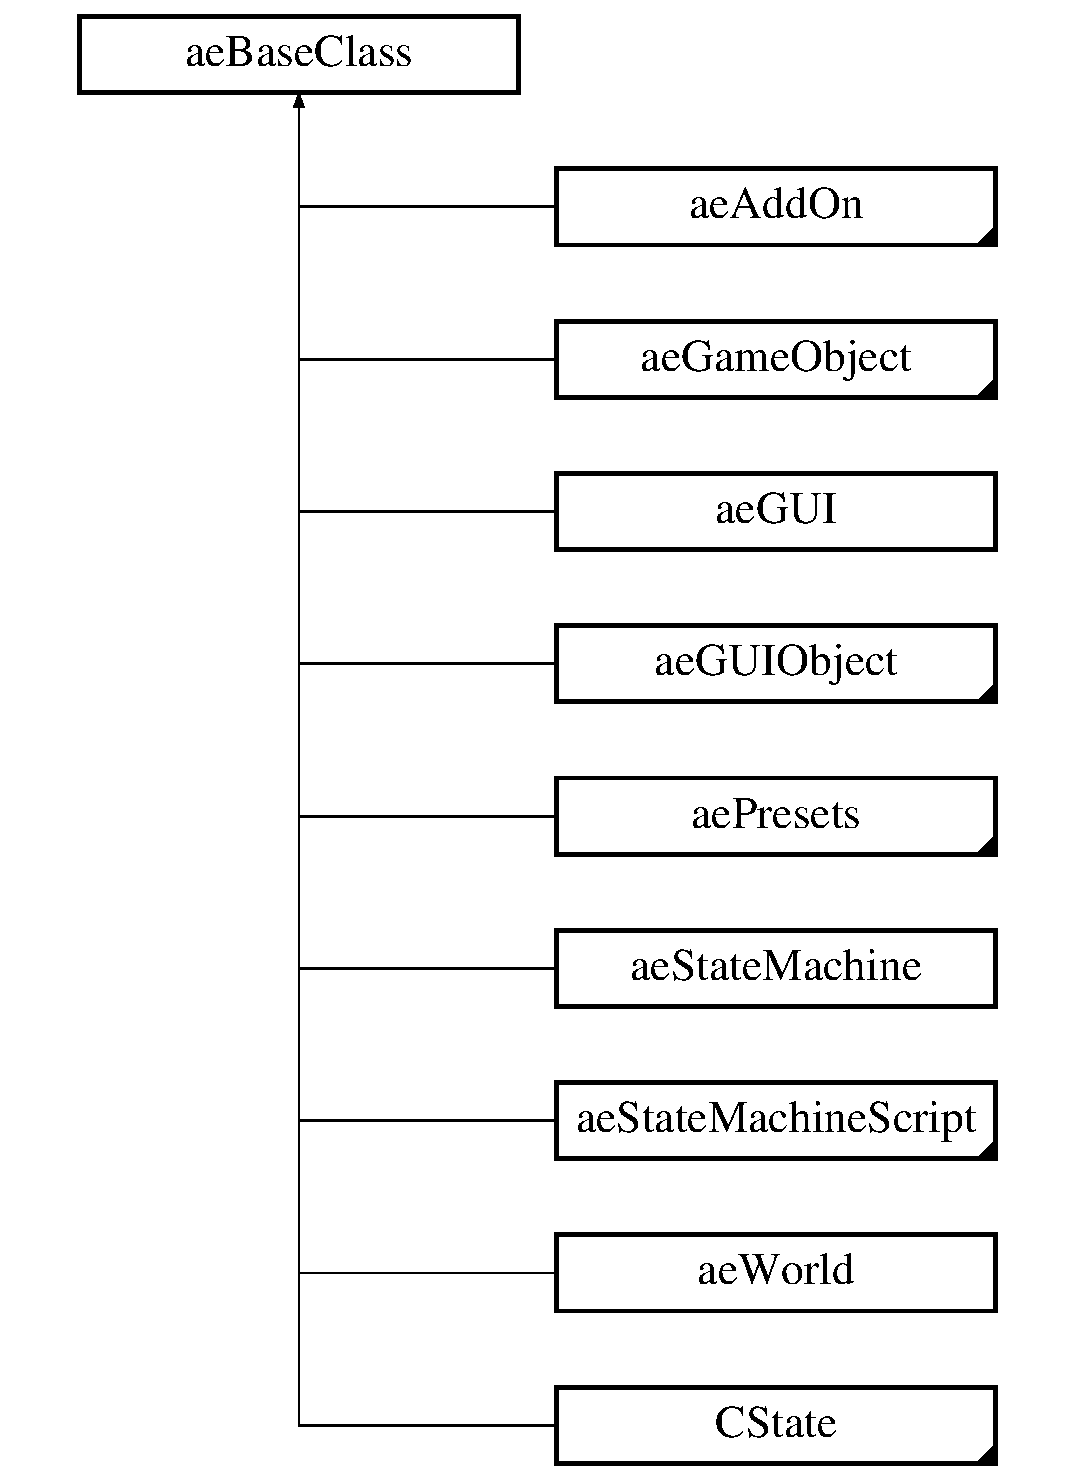
\includegraphics[height=10.000000cm]{classae_base_class}
\end{center}
\end{figure}
\subsection*{Public Member Functions}
\begin{DoxyCompactItemize}
\item 
\hyperlink{classae_base_class_a950b98d9d33b3b6aefb6ada8d42d080e}{ae\+Base\+Class} ()\hypertarget{classae_base_class_a950b98d9d33b3b6aefb6ada8d42d080e}{}\label{classae_base_class_a950b98d9d33b3b6aefb6ada8d42d080e}

\begin{DoxyCompactList}\small\item\em Default constructor. \end{DoxyCompactList}\item 
virtual \hyperlink{classae_base_class_ae6d0c4d413b54974121c683b26837df5}{$\sim$ae\+Base\+Class} ()\hypertarget{classae_base_class_ae6d0c4d413b54974121c683b26837df5}{}\label{classae_base_class_ae6d0c4d413b54974121c683b26837df5}

\begin{DoxyCompactList}\small\item\em Destructor. \end{DoxyCompactList}\item 
virtual void \hyperlink{classae_base_class_a8494fd89ce504af1b99de8cc8745f263}{Destroy} ()=0\hypertarget{classae_base_class_a8494fd89ce504af1b99de8cc8745f263}{}\label{classae_base_class_a8494fd89ce504af1b99de8cc8745f263}

\begin{DoxyCompactList}\small\item\em Destroys this object. \end{DoxyCompactList}\item 
\hyperlink{_base_class_8h_aded8224779c70fab5084220935d672bb}{Class\+Id} \hyperlink{classae_base_class_a9459c8bf81682fca6e12e1d85218c867}{Get\+Class\+ID} ()
\begin{DoxyCompactList}\small\item\em Gets the identifier. \end{DoxyCompactList}\item 
void \hyperlink{classae_base_class_aa53bf580448bdd8b7150974bf2bc195c}{Set\+Parent} (\hyperlink{classae_base_class}{ae\+Base\+Class} $\ast$p\+New\+Parent)
\begin{DoxyCompactList}\small\item\em Sets as parent. \end{DoxyCompactList}\item 
\hyperlink{classae_base_class}{ae\+Base\+Class} $\ast$ \hyperlink{classae_base_class_aa045d5ebc0492ccf0e1fc61083228fc5}{Get\+Parent} ()
\begin{DoxyCompactList}\small\item\em Gets the parent of this item. \end{DoxyCompactList}\end{DoxyCompactItemize}
\subsection*{Protected Attributes}
\begin{DoxyCompactItemize}
\item 
\hyperlink{_base_class_8h_aded8224779c70fab5084220935d672bb}{Class\+Id} \hyperlink{classae_base_class_a5e50065d7728452366fdedcc572a9815}{m\+\_\+n\+Class\+ID}\hypertarget{classae_base_class_a5e50065d7728452366fdedcc572a9815}{}\label{classae_base_class_a5e50065d7728452366fdedcc572a9815}

\begin{DoxyCompactList}\small\item\em Identifier for the class. \end{DoxyCompactList}\item 
\hyperlink{classae_base_class}{ae\+Base\+Class} $\ast$ \hyperlink{classae_base_class_a49e9c52f5fe5526b0a15f20f9e880dda}{m\+\_\+p\+Parent}\hypertarget{classae_base_class_a49e9c52f5fe5526b0a15f20f9e880dda}{}\label{classae_base_class_a49e9c52f5fe5526b0a15f20f9e880dda}

\begin{DoxyCompactList}\small\item\em The parent. \end{DoxyCompactList}\end{DoxyCompactItemize}


\subsection{Detailed Description}
A base class. 

\subsection{Member Function Documentation}
\index{ae\+Base\+Class@{ae\+Base\+Class}!Get\+Class\+ID@{Get\+Class\+ID}}
\index{Get\+Class\+ID@{Get\+Class\+ID}!ae\+Base\+Class@{ae\+Base\+Class}}
\subsubsection[{\texorpdfstring{Get\+Class\+I\+D()}{GetClassID()}}]{\setlength{\rightskip}{0pt plus 5cm}{\bf Class\+Id} ae\+Base\+Class\+::\+Get\+Class\+ID (
\begin{DoxyParamCaption}
{}
\end{DoxyParamCaption}
)}\hypertarget{classae_base_class_a9459c8bf81682fca6e12e1d85218c867}{}\label{classae_base_class_a9459c8bf81682fca6e12e1d85218c867}


Gets the identifier. 

\begin{DoxyReturn}{Returns}
The identifier. 
\end{DoxyReturn}
\index{ae\+Base\+Class@{ae\+Base\+Class}!Get\+Parent@{Get\+Parent}}
\index{Get\+Parent@{Get\+Parent}!ae\+Base\+Class@{ae\+Base\+Class}}
\subsubsection[{\texorpdfstring{Get\+Parent()}{GetParent()}}]{\setlength{\rightskip}{0pt plus 5cm}{\bf ae\+Base\+Class} $\ast$ ae\+Base\+Class\+::\+Get\+Parent (
\begin{DoxyParamCaption}
{}
\end{DoxyParamCaption}
)\hspace{0.3cm}{\ttfamily [inline]}}\hypertarget{classae_base_class_aa045d5ebc0492ccf0e1fc61083228fc5}{}\label{classae_base_class_aa045d5ebc0492ccf0e1fc61083228fc5}


Gets the parent of this item. 

\begin{DoxyReturn}{Returns}
null if it fails, else the parent. 
\end{DoxyReturn}
\index{ae\+Base\+Class@{ae\+Base\+Class}!Set\+Parent@{Set\+Parent}}
\index{Set\+Parent@{Set\+Parent}!ae\+Base\+Class@{ae\+Base\+Class}}
\subsubsection[{\texorpdfstring{Set\+Parent(ae\+Base\+Class $\ast$p\+New\+Parent)}{SetParent(aeBaseClass *pNewParent)}}]{\setlength{\rightskip}{0pt plus 5cm}void ae\+Base\+Class\+::\+Set\+Parent (
\begin{DoxyParamCaption}
\item[{{\bf ae\+Base\+Class} $\ast$}]{p\+New\+Parent}
\end{DoxyParamCaption}
)\hspace{0.3cm}{\ttfamily [inline]}}\hypertarget{classae_base_class_aa53bf580448bdd8b7150974bf2bc195c}{}\label{classae_base_class_aa53bf580448bdd8b7150974bf2bc195c}


Sets as parent. 


\begin{DoxyParams}[1]{Parameters}
\mbox{\tt in,out}  & {\em p\+New\+Parent} & If non-\/null, the new parent. \\
\hline
\end{DoxyParams}


The documentation for this class was generated from the following files\+:\begin{DoxyCompactItemize}
\item 
C\+:/\+Users/\+Alvaro Estrada/\+Documents/\+Visual Studio 2015/\+Projects/\+R\+T\+S\+\_\+\+A\+E/\+R\+T\+S\+\_\+\+A\+E/\+Game/\hyperlink{_base_class_8h}{Base\+Class.\+h}\item 
C\+:/\+Users/\+Alvaro Estrada/\+Documents/\+Visual Studio 2015/\+Projects/\+R\+T\+S\+\_\+\+A\+E/\+R\+T\+S\+\_\+\+A\+E/\+Game/Base\+Class.\+cpp\end{DoxyCompactItemize}

\hypertarget{classae_b_f_s_path_finder}{}\section{ae\+B\+F\+S\+Path\+Finder Class Reference}
\label{classae_b_f_s_path_finder}\index{ae\+B\+F\+S\+Path\+Finder@{ae\+B\+F\+S\+Path\+Finder}}
Inheritance diagram for ae\+B\+F\+S\+Path\+Finder\+:\begin{figure}[H]
\begin{center}
\leavevmode
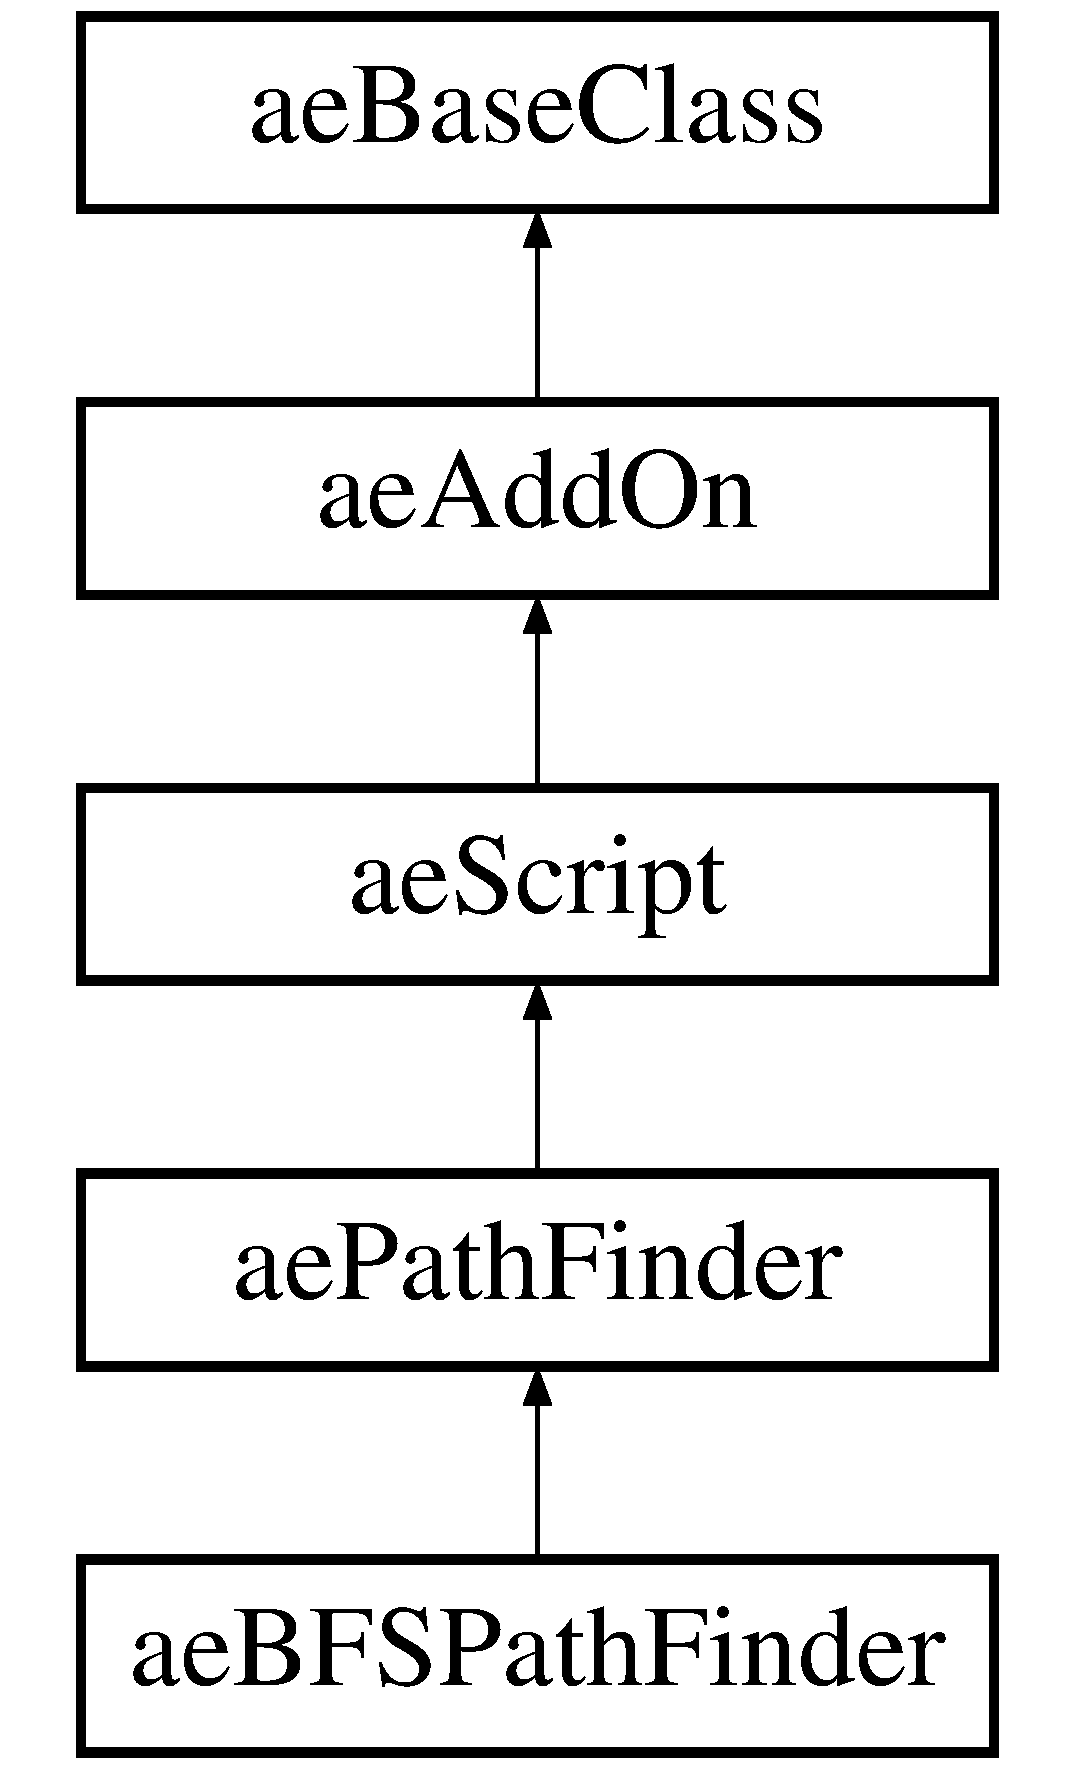
\includegraphics[height=5.000000cm]{classae_b_f_s_path_finder}
\end{center}
\end{figure}
\subsection*{Public Member Functions}
\begin{DoxyCompactItemize}
\item 
{\bfseries ae\+B\+F\+S\+Path\+Finder} (\hyperlink{classae_tiled_map}{ae\+Tiled\+Map} $\ast$p\+Map)\hypertarget{classae_b_f_s_path_finder_a6dabc113b1ef3ac90848ae78b8be5113}{}\label{classae_b_f_s_path_finder_a6dabc113b1ef3ac90848ae78b8be5113}

\item 
virtual int \hyperlink{classae_b_f_s_path_finder_a23a16f3e98f5c9fc3a6f56a26a7bf170}{Init} (\hyperlink{classae_base_class}{ae\+Base\+Class} $\ast$p\+Parent)
\begin{DoxyCompactList}\small\item\em Initializes with the given parent pointer. \end{DoxyCompactList}\item 
virtual void \hyperlink{classae_b_f_s_path_finder_a8221d21fdac79228e84aa104d30ee169}{Destroy} ()\hypertarget{classae_b_f_s_path_finder_a8221d21fdac79228e84aa104d30ee169}{}\label{classae_b_f_s_path_finder_a8221d21fdac79228e84aa104d30ee169}

\begin{DoxyCompactList}\small\item\em Destroys this object. \end{DoxyCompactList}\item 
virtual void \hyperlink{classae_b_f_s_path_finder_a00ddec6c4b37a3df127d1354cbc37635}{Update} (float f\+Delta)
\begin{DoxyCompactList}\small\item\em Updates the given f\+Delta. \end{DoxyCompactList}\item 
virtual void \hyperlink{classae_b_f_s_path_finder_a21efc2e873dd066f012ce0ef972a4a85}{Render} (\hyperlink{classae_core_1_1ae_renderer}{ae\+Renderer} $\ast$p\+Renderer)
\begin{DoxyCompactList}\small\item\em Renders the given Renderer pointer. \end{DoxyCompactList}\item 
virtual void \hyperlink{classae_b_f_s_path_finder_a3084aac6b6af17754b857915670a831e}{Reset} ()\hypertarget{classae_b_f_s_path_finder_a3084aac6b6af17754b857915670a831e}{}\label{classae_b_f_s_path_finder_a3084aac6b6af17754b857915670a831e}

\begin{DoxyCompactList}\small\item\em Resets this object. \end{DoxyCompactList}\end{DoxyCompactItemize}
\subsection*{Protected Member Functions}
\begin{DoxyCompactItemize}
\item 
virtual void \hyperlink{classae_b_f_s_path_finder_a92683a0590099c03c5a0527fc7d11ae0}{Visit\+Grid\+Node} (\hyperlink{namespaceae_core_a862bc39eb87cfabca273f49e2a920129}{int32} x, \hyperlink{namespaceae_core_a862bc39eb87cfabca273f49e2a920129}{int32} y)
\begin{DoxyCompactList}\small\item\em Marks a node as visited. \end{DoxyCompactList}\item 
virtual void \hyperlink{classae_b_f_s_path_finder_a514fe666fadd79cdd6d44af875fb5900}{Set\+Final\+Node} (\hyperlink{namespaceae_core_a862bc39eb87cfabca273f49e2a920129}{int32} x, \hyperlink{namespaceae_core_a862bc39eb87cfabca273f49e2a920129}{int32} y)
\begin{DoxyCompactList}\small\item\em Sets final node. \end{DoxyCompactList}\item 
virtual Walk\+State\+ID \hyperlink{classae_b_f_s_path_finder_a92b13a108bd1151d796dba5a3426704c}{Give\+A\+Step} ()
\begin{DoxyCompactList}\small\item\em Give a step. \end{DoxyCompactList}\end{DoxyCompactItemize}
\subsection*{Additional Inherited Members}


\subsection{Member Function Documentation}
\index{ae\+B\+F\+S\+Path\+Finder@{ae\+B\+F\+S\+Path\+Finder}!Give\+A\+Step@{Give\+A\+Step}}
\index{Give\+A\+Step@{Give\+A\+Step}!ae\+B\+F\+S\+Path\+Finder@{ae\+B\+F\+S\+Path\+Finder}}
\subsubsection[{\texorpdfstring{Give\+A\+Step()}{GiveAStep()}}]{\setlength{\rightskip}{0pt plus 5cm}Walk\+State\+ID ae\+B\+F\+S\+Path\+Finder\+::\+Give\+A\+Step (
\begin{DoxyParamCaption}
{}
\end{DoxyParamCaption}
)\hspace{0.3cm}{\ttfamily [protected]}, {\ttfamily [virtual]}}\hypertarget{classae_b_f_s_path_finder_a92b13a108bd1151d796dba5a3426704c}{}\label{classae_b_f_s_path_finder_a92b13a108bd1151d796dba5a3426704c}


Give a step. 

\begin{DoxyReturn}{Returns}
A Walk\+State\+ID. 
\end{DoxyReturn}


Implements \hyperlink{classae_path_finder_a49332ee3be744cac1ece9ffd503ca218}{ae\+Path\+Finder}.

\index{ae\+B\+F\+S\+Path\+Finder@{ae\+B\+F\+S\+Path\+Finder}!Init@{Init}}
\index{Init@{Init}!ae\+B\+F\+S\+Path\+Finder@{ae\+B\+F\+S\+Path\+Finder}}
\subsubsection[{\texorpdfstring{Init(ae\+Base\+Class $\ast$p\+Parent)}{Init(aeBaseClass *pParent)}}]{\setlength{\rightskip}{0pt plus 5cm}int ae\+B\+F\+S\+Path\+Finder\+::\+Init (
\begin{DoxyParamCaption}
\item[{{\bf ae\+Base\+Class} $\ast$}]{p\+Parent}
\end{DoxyParamCaption}
)\hspace{0.3cm}{\ttfamily [virtual]}}\hypertarget{classae_b_f_s_path_finder_a23a16f3e98f5c9fc3a6f56a26a7bf170}{}\label{classae_b_f_s_path_finder_a23a16f3e98f5c9fc3a6f56a26a7bf170}


Initializes with the given parent pointer. 


\begin{DoxyParams}[1]{Parameters}
\mbox{\tt in,out}  & {\em p\+Parent} & If non-\/null, the parent.\\
\hline
\end{DoxyParams}
\begin{DoxyReturn}{Returns}
An int. 
\end{DoxyReturn}


Reimplemented from \hyperlink{classae_path_finder_a3395375f3de8f3f55d7b780ff6815806}{ae\+Path\+Finder}.

\index{ae\+B\+F\+S\+Path\+Finder@{ae\+B\+F\+S\+Path\+Finder}!Render@{Render}}
\index{Render@{Render}!ae\+B\+F\+S\+Path\+Finder@{ae\+B\+F\+S\+Path\+Finder}}
\subsubsection[{\texorpdfstring{Render(ae\+Renderer $\ast$p\+Renderer)}{Render(aeRenderer *pRenderer)}}]{\setlength{\rightskip}{0pt plus 5cm}void ae\+B\+F\+S\+Path\+Finder\+::\+Render (
\begin{DoxyParamCaption}
\item[{{\bf ae\+Renderer} $\ast$}]{p\+Renderer}
\end{DoxyParamCaption}
)\hspace{0.3cm}{\ttfamily [virtual]}}\hypertarget{classae_b_f_s_path_finder_a21efc2e873dd066f012ce0ef972a4a85}{}\label{classae_b_f_s_path_finder_a21efc2e873dd066f012ce0ef972a4a85}


Renders the given Renderer pointer. 


\begin{DoxyParams}[1]{Parameters}
\mbox{\tt in,out}  & {\em p\+Renderer} & If non-\/null, the renderer. \\
\hline
\end{DoxyParams}


Reimplemented from \hyperlink{classae_add_on_ab6bed56009b9c92df8ae017a27587dc3}{ae\+Add\+On}.

\index{ae\+B\+F\+S\+Path\+Finder@{ae\+B\+F\+S\+Path\+Finder}!Set\+Final\+Node@{Set\+Final\+Node}}
\index{Set\+Final\+Node@{Set\+Final\+Node}!ae\+B\+F\+S\+Path\+Finder@{ae\+B\+F\+S\+Path\+Finder}}
\subsubsection[{\texorpdfstring{Set\+Final\+Node(int32 x, int32 y)}{SetFinalNode(int32 x, int32 y)}}]{\setlength{\rightskip}{0pt plus 5cm}void ae\+B\+F\+S\+Path\+Finder\+::\+Set\+Final\+Node (
\begin{DoxyParamCaption}
\item[{{\bf int32}}]{x, }
\item[{{\bf int32}}]{y}
\end{DoxyParamCaption}
)\hspace{0.3cm}{\ttfamily [protected]}, {\ttfamily [virtual]}}\hypertarget{classae_b_f_s_path_finder_a514fe666fadd79cdd6d44af875fb5900}{}\label{classae_b_f_s_path_finder_a514fe666fadd79cdd6d44af875fb5900}


Sets final node. 


\begin{DoxyParams}{Parameters}
{\em x} & The x coordinate. \\
\hline
{\em y} & The y coordinate. \\
\hline
\end{DoxyParams}
\index{ae\+B\+F\+S\+Path\+Finder@{ae\+B\+F\+S\+Path\+Finder}!Update@{Update}}
\index{Update@{Update}!ae\+B\+F\+S\+Path\+Finder@{ae\+B\+F\+S\+Path\+Finder}}
\subsubsection[{\texorpdfstring{Update(float f\+Delta)}{Update(float fDelta)}}]{\setlength{\rightskip}{0pt plus 5cm}void ae\+B\+F\+S\+Path\+Finder\+::\+Update (
\begin{DoxyParamCaption}
\item[{float}]{f\+Delta}
\end{DoxyParamCaption}
)\hspace{0.3cm}{\ttfamily [virtual]}}\hypertarget{classae_b_f_s_path_finder_a00ddec6c4b37a3df127d1354cbc37635}{}\label{classae_b_f_s_path_finder_a00ddec6c4b37a3df127d1354cbc37635}


Updates the given f\+Delta. 


\begin{DoxyParams}{Parameters}
{\em f\+Delta} & The delta. \\
\hline
\end{DoxyParams}


Implements \hyperlink{classae_add_on_a51caa4b8680206495ea671e71991e231}{ae\+Add\+On}.

\index{ae\+B\+F\+S\+Path\+Finder@{ae\+B\+F\+S\+Path\+Finder}!Visit\+Grid\+Node@{Visit\+Grid\+Node}}
\index{Visit\+Grid\+Node@{Visit\+Grid\+Node}!ae\+B\+F\+S\+Path\+Finder@{ae\+B\+F\+S\+Path\+Finder}}
\subsubsection[{\texorpdfstring{Visit\+Grid\+Node(int32 x, int32 y)}{VisitGridNode(int32 x, int32 y)}}]{\setlength{\rightskip}{0pt plus 5cm}void ae\+B\+F\+S\+Path\+Finder\+::\+Visit\+Grid\+Node (
\begin{DoxyParamCaption}
\item[{{\bf int32}}]{x, }
\item[{{\bf int32}}]{y}
\end{DoxyParamCaption}
)\hspace{0.3cm}{\ttfamily [protected]}, {\ttfamily [virtual]}}\hypertarget{classae_b_f_s_path_finder_a92683a0590099c03c5a0527fc7d11ae0}{}\label{classae_b_f_s_path_finder_a92683a0590099c03c5a0527fc7d11ae0}


Marks a node as visited. 


\begin{DoxyParams}{Parameters}
{\em x} & The x coordinate. \\
\hline
{\em y} & The y coordinate. \\
\hline
\end{DoxyParams}


Implements \hyperlink{classae_path_finder_a4ccfa19ff344b9f4827dbeab18c4efab}{ae\+Path\+Finder}.



The documentation for this class was generated from the following files\+:\begin{DoxyCompactItemize}
\item 
C\+:/\+Users/\+Alvaro Estrada/\+Documents/\+Visual Studio 2015/\+Projects/\+R\+T\+S\+\_\+\+A\+E/\+R\+T\+S\+\_\+\+A\+E/\+Game/\hyperlink{_breadth_first_search_8h}{Breadth\+First\+Search.\+h}\item 
C\+:/\+Users/\+Alvaro Estrada/\+Documents/\+Visual Studio 2015/\+Projects/\+R\+T\+S\+\_\+\+A\+E/\+R\+T\+S\+\_\+\+A\+E/\+Game/\hyperlink{_breadth_first_search_8cpp}{Breadth\+First\+Search.\+cpp}\end{DoxyCompactItemize}

\hypertarget{classae_bst_f_s_path_finder}{}\section{ae\+Bst\+F\+S\+Path\+Finder Class Reference}
\label{classae_bst_f_s_path_finder}\index{ae\+Bst\+F\+S\+Path\+Finder@{ae\+Bst\+F\+S\+Path\+Finder}}
Inheritance diagram for ae\+Bst\+F\+S\+Path\+Finder\+:\begin{figure}[H]
\begin{center}
\leavevmode
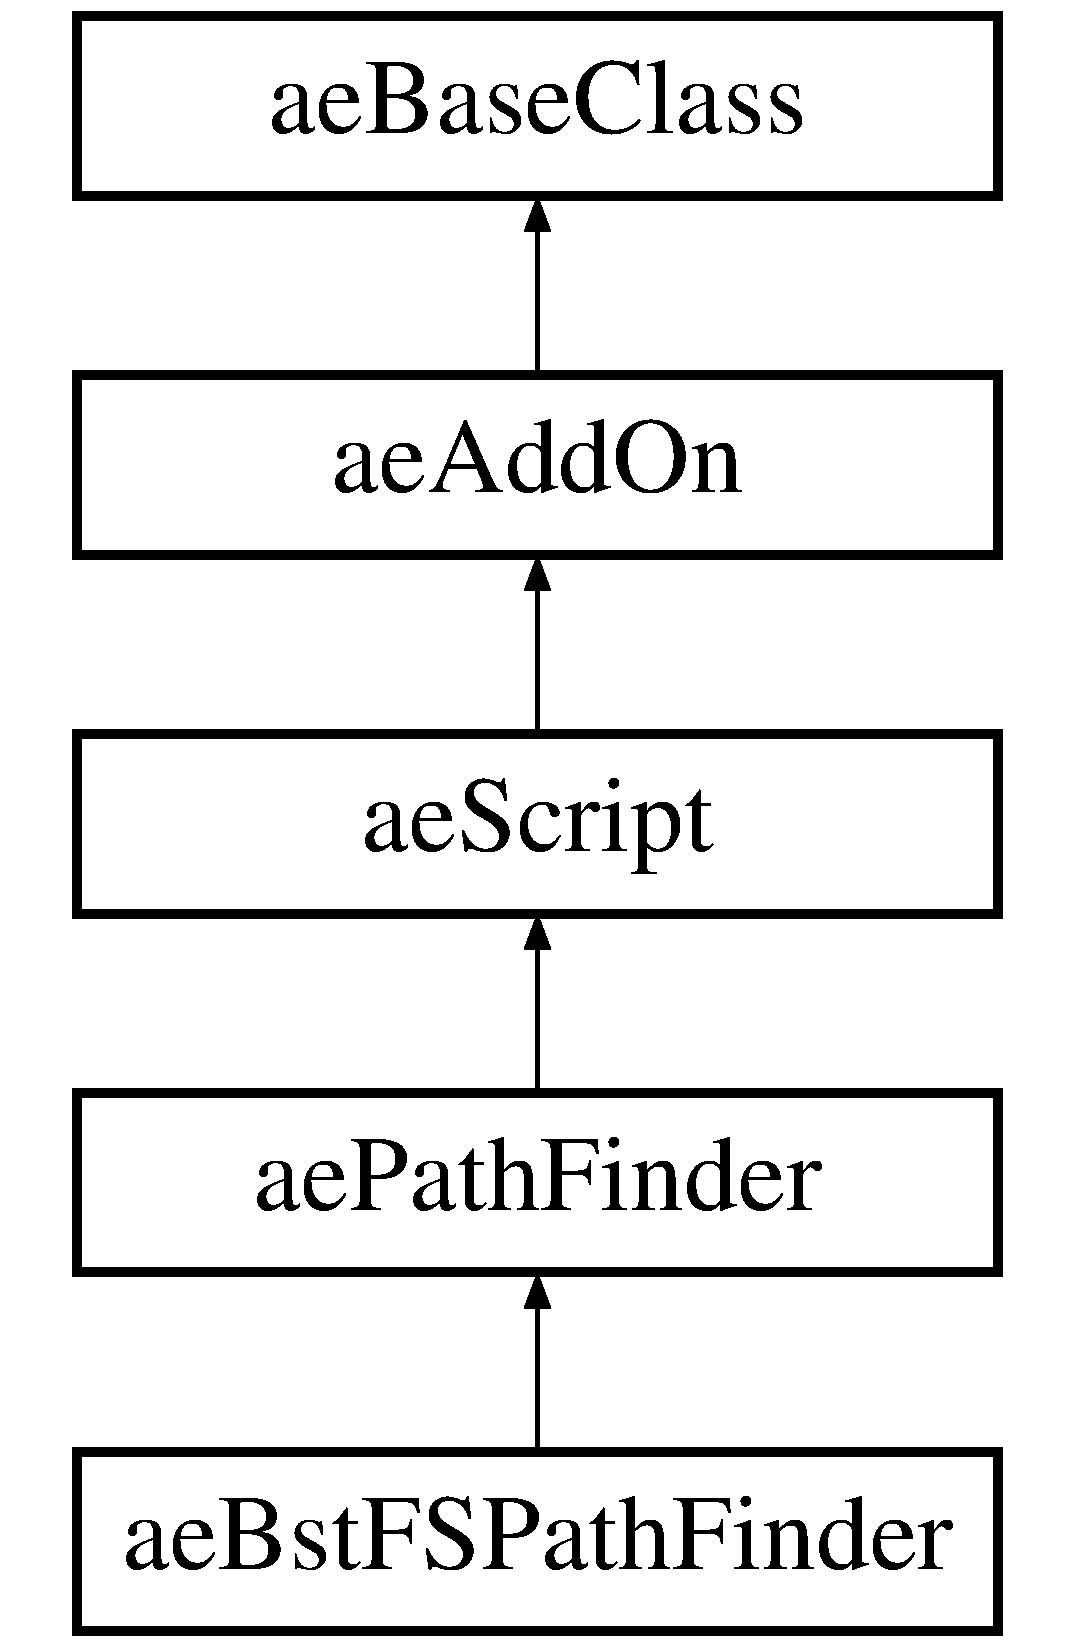
\includegraphics[height=5.000000cm]{classae_bst_f_s_path_finder}
\end{center}
\end{figure}
\subsection*{Public Member Functions}
\begin{DoxyCompactItemize}
\item 
{\bfseries ae\+Bst\+F\+S\+Path\+Finder} (\hyperlink{classae_tiled_map}{ae\+Tiled\+Map} $\ast$p\+Map)\hypertarget{classae_bst_f_s_path_finder_a9f7b5e5aaa29bfe2502186fa46101df6}{}\label{classae_bst_f_s_path_finder_a9f7b5e5aaa29bfe2502186fa46101df6}

\item 
virtual int \hyperlink{classae_bst_f_s_path_finder_a83e0028b1394744dc56b703532a88b40}{Init} (\hyperlink{classae_base_class}{ae\+Base\+Class} $\ast$p\+Parent)
\begin{DoxyCompactList}\small\item\em Initializes with the given parent pointer. \end{DoxyCompactList}\item 
virtual void \hyperlink{classae_bst_f_s_path_finder_a9d9c30e5ce6cf6b00792ef59dbaef8b9}{Destroy} ()\hypertarget{classae_bst_f_s_path_finder_a9d9c30e5ce6cf6b00792ef59dbaef8b9}{}\label{classae_bst_f_s_path_finder_a9d9c30e5ce6cf6b00792ef59dbaef8b9}

\begin{DoxyCompactList}\small\item\em Destroys this object. \end{DoxyCompactList}\item 
virtual void \hyperlink{classae_bst_f_s_path_finder_a27dd4200f183349f605407278de0d086}{Update} (float f\+Delta)
\begin{DoxyCompactList}\small\item\em Updates the given f\+Delta. \end{DoxyCompactList}\item 
virtual void \hyperlink{classae_bst_f_s_path_finder_a6c3646502a67f145cd849392918b4c4b}{Render} (\hyperlink{classae_core_1_1ae_renderer}{ae\+Renderer} $\ast$p\+Renderer)
\begin{DoxyCompactList}\small\item\em Renders the given Renderer pointer. \end{DoxyCompactList}\item 
virtual void \hyperlink{classae_bst_f_s_path_finder_a31dcc8f08f56766c97b9054340faaaec}{Reset} ()\hypertarget{classae_bst_f_s_path_finder_a31dcc8f08f56766c97b9054340faaaec}{}\label{classae_bst_f_s_path_finder_a31dcc8f08f56766c97b9054340faaaec}

\begin{DoxyCompactList}\small\item\em Resets this object. \end{DoxyCompactList}\end{DoxyCompactItemize}
\subsection*{Protected Member Functions}
\begin{DoxyCompactItemize}
\item 
virtual void \hyperlink{classae_bst_f_s_path_finder_ae46add3c2ab1986423288bde7f92bcf0}{Visit\+Grid\+Node} (\hyperlink{namespaceae_core_a862bc39eb87cfabca273f49e2a920129}{int32} x, \hyperlink{namespaceae_core_a862bc39eb87cfabca273f49e2a920129}{int32} y)
\begin{DoxyCompactList}\small\item\em Marks a node as visited. \end{DoxyCompactList}\item 
virtual void \hyperlink{classae_bst_f_s_path_finder_ad4cafbb4ca0786cd6c4a7e5381b0d3ec}{Set\+Final\+Node} (\hyperlink{namespaceae_core_a862bc39eb87cfabca273f49e2a920129}{int32} x, \hyperlink{namespaceae_core_a862bc39eb87cfabca273f49e2a920129}{int32} y)
\begin{DoxyCompactList}\small\item\em Sets final node. \end{DoxyCompactList}\item 
virtual Walk\+State\+ID \hyperlink{classae_bst_f_s_path_finder_a172082a7d5f6de9d5163991c076455ca}{Give\+A\+Step} ()
\begin{DoxyCompactList}\small\item\em Give a step. \end{DoxyCompactList}\end{DoxyCompactItemize}
\subsection*{Additional Inherited Members}


\subsection{Member Function Documentation}
\index{ae\+Bst\+F\+S\+Path\+Finder@{ae\+Bst\+F\+S\+Path\+Finder}!Give\+A\+Step@{Give\+A\+Step}}
\index{Give\+A\+Step@{Give\+A\+Step}!ae\+Bst\+F\+S\+Path\+Finder@{ae\+Bst\+F\+S\+Path\+Finder}}
\subsubsection[{\texorpdfstring{Give\+A\+Step()}{GiveAStep()}}]{\setlength{\rightskip}{0pt plus 5cm}Walk\+State\+ID ae\+Bst\+F\+S\+Path\+Finder\+::\+Give\+A\+Step (
\begin{DoxyParamCaption}
{}
\end{DoxyParamCaption}
)\hspace{0.3cm}{\ttfamily [protected]}, {\ttfamily [virtual]}}\hypertarget{classae_bst_f_s_path_finder_a172082a7d5f6de9d5163991c076455ca}{}\label{classae_bst_f_s_path_finder_a172082a7d5f6de9d5163991c076455ca}


Give a step. 

\begin{DoxyReturn}{Returns}
A Walk\+State\+ID. 
\end{DoxyReturn}


Implements \hyperlink{classae_path_finder_a49332ee3be744cac1ece9ffd503ca218}{ae\+Path\+Finder}.

\index{ae\+Bst\+F\+S\+Path\+Finder@{ae\+Bst\+F\+S\+Path\+Finder}!Init@{Init}}
\index{Init@{Init}!ae\+Bst\+F\+S\+Path\+Finder@{ae\+Bst\+F\+S\+Path\+Finder}}
\subsubsection[{\texorpdfstring{Init(ae\+Base\+Class $\ast$p\+Parent)}{Init(aeBaseClass *pParent)}}]{\setlength{\rightskip}{0pt plus 5cm}int ae\+Bst\+F\+S\+Path\+Finder\+::\+Init (
\begin{DoxyParamCaption}
\item[{{\bf ae\+Base\+Class} $\ast$}]{p\+Parent}
\end{DoxyParamCaption}
)\hspace{0.3cm}{\ttfamily [virtual]}}\hypertarget{classae_bst_f_s_path_finder_a83e0028b1394744dc56b703532a88b40}{}\label{classae_bst_f_s_path_finder_a83e0028b1394744dc56b703532a88b40}


Initializes with the given parent pointer. 


\begin{DoxyParams}[1]{Parameters}
\mbox{\tt in,out}  & {\em p\+Parent} & If non-\/null, the parent.\\
\hline
\end{DoxyParams}
\begin{DoxyReturn}{Returns}
An int. 
\end{DoxyReturn}


Reimplemented from \hyperlink{classae_path_finder_a3395375f3de8f3f55d7b780ff6815806}{ae\+Path\+Finder}.

\index{ae\+Bst\+F\+S\+Path\+Finder@{ae\+Bst\+F\+S\+Path\+Finder}!Render@{Render}}
\index{Render@{Render}!ae\+Bst\+F\+S\+Path\+Finder@{ae\+Bst\+F\+S\+Path\+Finder}}
\subsubsection[{\texorpdfstring{Render(ae\+Renderer $\ast$p\+Renderer)}{Render(aeRenderer *pRenderer)}}]{\setlength{\rightskip}{0pt plus 5cm}void ae\+Bst\+F\+S\+Path\+Finder\+::\+Render (
\begin{DoxyParamCaption}
\item[{{\bf ae\+Renderer} $\ast$}]{p\+Renderer}
\end{DoxyParamCaption}
)\hspace{0.3cm}{\ttfamily [virtual]}}\hypertarget{classae_bst_f_s_path_finder_a6c3646502a67f145cd849392918b4c4b}{}\label{classae_bst_f_s_path_finder_a6c3646502a67f145cd849392918b4c4b}


Renders the given Renderer pointer. 


\begin{DoxyParams}[1]{Parameters}
\mbox{\tt in,out}  & {\em p\+Renderer} & If non-\/null, the renderer. \\
\hline
\end{DoxyParams}


Reimplemented from \hyperlink{classae_add_on_ab6bed56009b9c92df8ae017a27587dc3}{ae\+Add\+On}.

\index{ae\+Bst\+F\+S\+Path\+Finder@{ae\+Bst\+F\+S\+Path\+Finder}!Set\+Final\+Node@{Set\+Final\+Node}}
\index{Set\+Final\+Node@{Set\+Final\+Node}!ae\+Bst\+F\+S\+Path\+Finder@{ae\+Bst\+F\+S\+Path\+Finder}}
\subsubsection[{\texorpdfstring{Set\+Final\+Node(int32 x, int32 y)}{SetFinalNode(int32 x, int32 y)}}]{\setlength{\rightskip}{0pt plus 5cm}void ae\+Bst\+F\+S\+Path\+Finder\+::\+Set\+Final\+Node (
\begin{DoxyParamCaption}
\item[{{\bf int32}}]{x, }
\item[{{\bf int32}}]{y}
\end{DoxyParamCaption}
)\hspace{0.3cm}{\ttfamily [protected]}, {\ttfamily [virtual]}}\hypertarget{classae_bst_f_s_path_finder_ad4cafbb4ca0786cd6c4a7e5381b0d3ec}{}\label{classae_bst_f_s_path_finder_ad4cafbb4ca0786cd6c4a7e5381b0d3ec}


Sets final node. 


\begin{DoxyParams}{Parameters}
{\em x} & The x coordinate. \\
\hline
{\em y} & The y coordinate. \\
\hline
\end{DoxyParams}
\index{ae\+Bst\+F\+S\+Path\+Finder@{ae\+Bst\+F\+S\+Path\+Finder}!Update@{Update}}
\index{Update@{Update}!ae\+Bst\+F\+S\+Path\+Finder@{ae\+Bst\+F\+S\+Path\+Finder}}
\subsubsection[{\texorpdfstring{Update(float f\+Delta)}{Update(float fDelta)}}]{\setlength{\rightskip}{0pt plus 5cm}void ae\+Bst\+F\+S\+Path\+Finder\+::\+Update (
\begin{DoxyParamCaption}
\item[{float}]{f\+Delta}
\end{DoxyParamCaption}
)\hspace{0.3cm}{\ttfamily [virtual]}}\hypertarget{classae_bst_f_s_path_finder_a27dd4200f183349f605407278de0d086}{}\label{classae_bst_f_s_path_finder_a27dd4200f183349f605407278de0d086}


Updates the given f\+Delta. 


\begin{DoxyParams}{Parameters}
{\em f\+Delta} & The delta. \\
\hline
\end{DoxyParams}


Implements \hyperlink{classae_add_on_a51caa4b8680206495ea671e71991e231}{ae\+Add\+On}.

\index{ae\+Bst\+F\+S\+Path\+Finder@{ae\+Bst\+F\+S\+Path\+Finder}!Visit\+Grid\+Node@{Visit\+Grid\+Node}}
\index{Visit\+Grid\+Node@{Visit\+Grid\+Node}!ae\+Bst\+F\+S\+Path\+Finder@{ae\+Bst\+F\+S\+Path\+Finder}}
\subsubsection[{\texorpdfstring{Visit\+Grid\+Node(int32 x, int32 y)}{VisitGridNode(int32 x, int32 y)}}]{\setlength{\rightskip}{0pt plus 5cm}void ae\+Bst\+F\+S\+Path\+Finder\+::\+Visit\+Grid\+Node (
\begin{DoxyParamCaption}
\item[{{\bf int32}}]{x, }
\item[{{\bf int32}}]{y}
\end{DoxyParamCaption}
)\hspace{0.3cm}{\ttfamily [protected]}, {\ttfamily [virtual]}}\hypertarget{classae_bst_f_s_path_finder_ae46add3c2ab1986423288bde7f92bcf0}{}\label{classae_bst_f_s_path_finder_ae46add3c2ab1986423288bde7f92bcf0}


Marks a node as visited. 


\begin{DoxyParams}{Parameters}
{\em x} & The x coordinate. \\
\hline
{\em y} & The y coordinate. \\
\hline
\end{DoxyParams}


Implements \hyperlink{classae_path_finder_a4ccfa19ff344b9f4827dbeab18c4efab}{ae\+Path\+Finder}.



The documentation for this class was generated from the following files\+:\begin{DoxyCompactItemize}
\item 
C\+:/\+Users/\+Alvaro Estrada/\+Documents/\+Visual Studio 2015/\+Projects/\+R\+T\+S\+\_\+\+A\+E/\+R\+T\+S\+\_\+\+A\+E/\+Game/Best\+First\+Search.\+h\item 
C\+:/\+Users/\+Alvaro Estrada/\+Documents/\+Visual Studio 2015/\+Projects/\+R\+T\+S\+\_\+\+A\+E/\+R\+T\+S\+\_\+\+A\+E/\+Game/Best\+First\+Search.\+cpp\end{DoxyCompactItemize}

\hypertarget{classae_button_script}{}\section{ae\+Button\+Script Class Reference}
\label{classae_button_script}\index{ae\+Button\+Script@{ae\+Button\+Script}}


A button script.  




{\ttfamily \#include $<$Button\+Script.\+h$>$}

Inheritance diagram for ae\+Button\+Script\+:\begin{figure}[H]
\begin{center}
\leavevmode
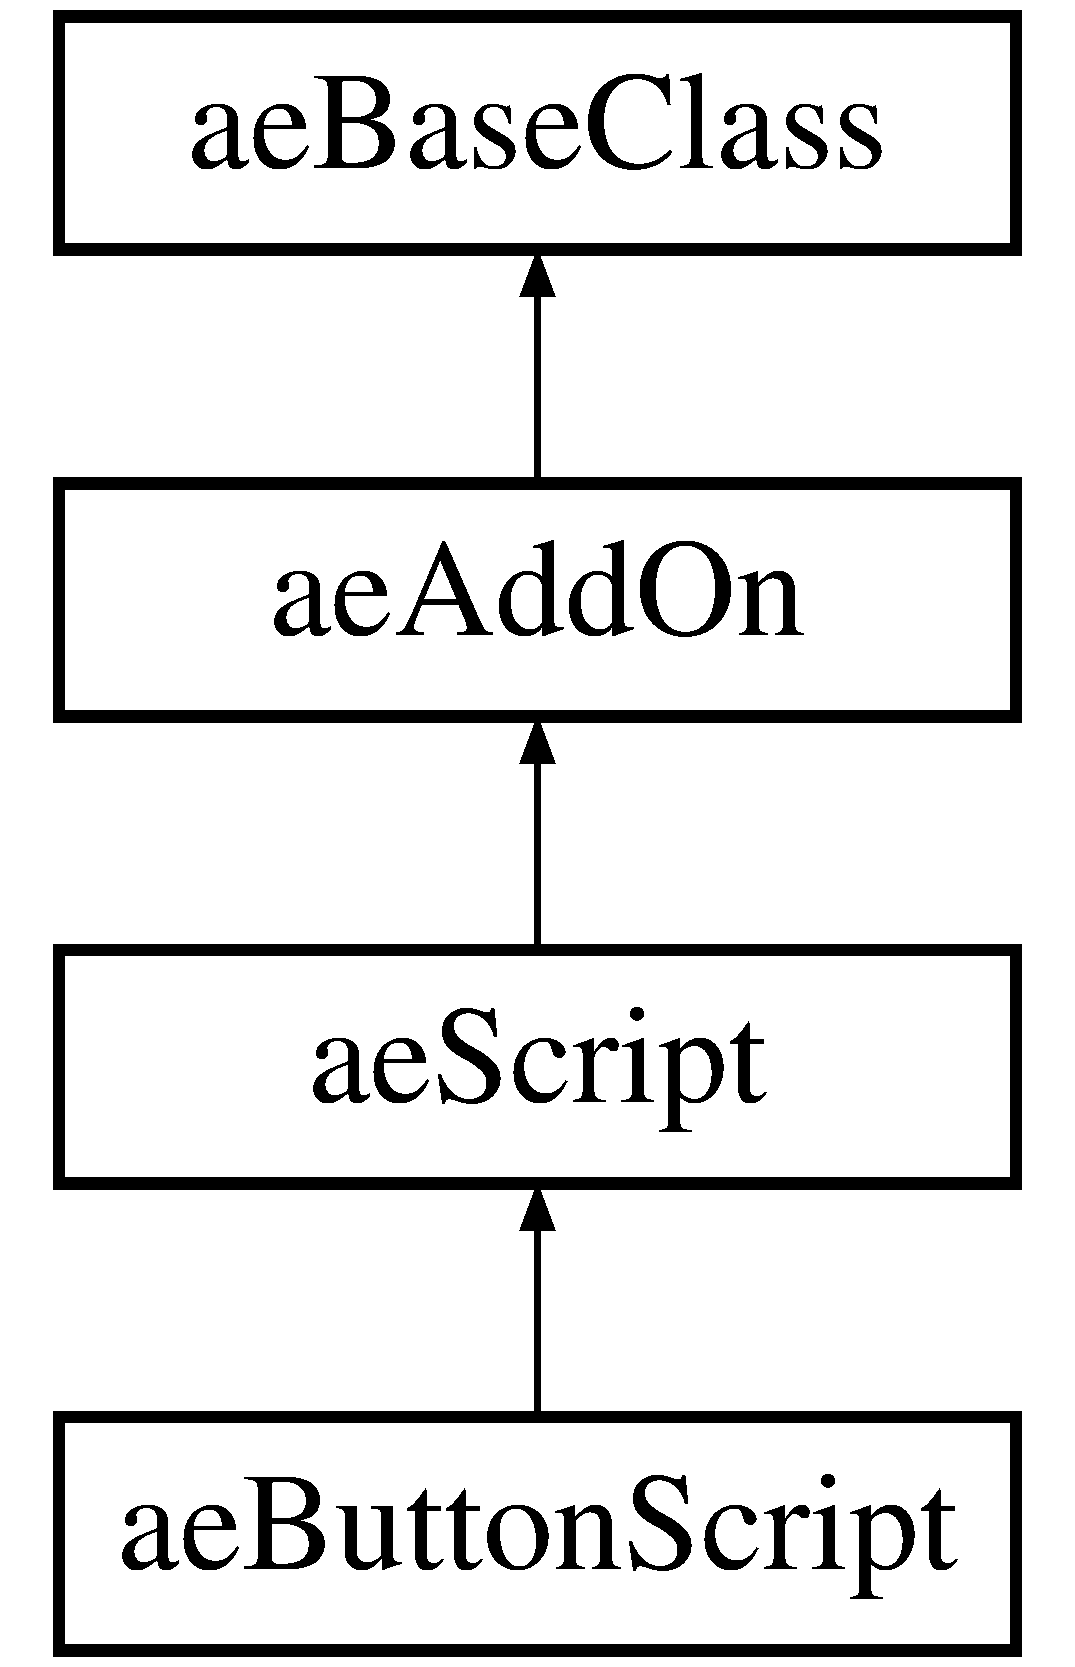
\includegraphics[height=4.000000cm]{classae_button_script}
\end{center}
\end{figure}
\subsection*{Public Member Functions}
\begin{DoxyCompactItemize}
\item 
virtual void \hyperlink{classae_button_script_a31b079712874fdb93a5dbb34de26c44c}{On\+Enter} ()\hypertarget{classae_button_script_a31b079712874fdb93a5dbb34de26c44c}{}\label{classae_button_script_a31b079712874fdb93a5dbb34de26c44c}

\begin{DoxyCompactList}\small\item\em Executes the enter action. \end{DoxyCompactList}\item 
virtual void \hyperlink{classae_button_script_a2a30b245d1a5b50618e0d5fe93340034}{On\+Exit} ()\hypertarget{classae_button_script_a2a30b245d1a5b50618e0d5fe93340034}{}\label{classae_button_script_a2a30b245d1a5b50618e0d5fe93340034}

\begin{DoxyCompactList}\small\item\em Executes the exit action. \end{DoxyCompactList}\item 
virtual void \hyperlink{classae_button_script_a637f94fac009f1db840c87e44c6549bc}{On\+Pressed} ()\hypertarget{classae_button_script_a637f94fac009f1db840c87e44c6549bc}{}\label{classae_button_script_a637f94fac009f1db840c87e44c6549bc}

\begin{DoxyCompactList}\small\item\em Executes the pressed action. \end{DoxyCompactList}\item 
virtual void \hyperlink{classae_button_script_ae8f1f681631336066515f9cc385b5383}{On\+Released} ()\hypertarget{classae_button_script_ae8f1f681631336066515f9cc385b5383}{}\label{classae_button_script_ae8f1f681631336066515f9cc385b5383}

\begin{DoxyCompactList}\small\item\em Executes the released action. \end{DoxyCompactList}\end{DoxyCompactItemize}
\subsection*{Additional Inherited Members}


\subsection{Detailed Description}
A button script. 

The documentation for this class was generated from the following files\+:\begin{DoxyCompactItemize}
\item 
C\+:/\+Users/\+Alvaro Estrada/\+Documents/\+Visual Studio 2015/\+Projects/\+R\+T\+S\+\_\+\+A\+E/\+R\+T\+S\+\_\+\+A\+E/\+Game/\hyperlink{_button_script_8h}{Button\+Script.\+h}\item 
C\+:/\+Users/\+Alvaro Estrada/\+Documents/\+Visual Studio 2015/\+Projects/\+R\+T\+S\+\_\+\+A\+E/\+R\+T\+S\+\_\+\+A\+E/\+Game/Button\+Script.\+cpp\end{DoxyCompactItemize}

\hypertarget{classae_core_1_1ae_clock}{}\section{ae\+Core\+:\+:ae\+Clock Class Reference}
\label{classae_core_1_1ae_clock}\index{ae\+Core\+::ae\+Clock@{ae\+Core\+::ae\+Clock}}


A high resolution timer.  




{\ttfamily \#include $<$Clock.\+h$>$}

\subsection*{Public Member Functions}
\begin{DoxyCompactItemize}
\item 
\hyperlink{classae_core_1_1ae_clock_acce423a302fdb8c3cbbdc9f16cc92b4d}{ae\+Clock} ()\hypertarget{classae_core_1_1ae_clock_acce423a302fdb8c3cbbdc9f16cc92b4d}{}\label{classae_core_1_1ae_clock_acce423a302fdb8c3cbbdc9f16cc92b4d}

\begin{DoxyCompactList}\small\item\em Default constructor. \end{DoxyCompactList}\item 
\hyperlink{classae_core_1_1ae_clock_ab5fb0b048af4531eb109d5e20759bdf0}{$\sim$ae\+Clock} ()\hypertarget{classae_core_1_1ae_clock_ab5fb0b048af4531eb109d5e20759bdf0}{}\label{classae_core_1_1ae_clock_ab5fb0b048af4531eb109d5e20759bdf0}

\begin{DoxyCompactList}\small\item\em Destructor. \end{DoxyCompactList}\item 
int \hyperlink{classae_core_1_1ae_clock_a43da19cb58c81e07cddb5097a191748d}{Init} ()
\begin{DoxyCompactList}\small\item\em Gets 0 if it was initialized correctly, otherwise, it will get an error number. \end{DoxyCompactList}\item 
void \hyperlink{classae_core_1_1ae_clock_a87f4a727d750d3cfbbad04317ac0d0d2}{Destroy} ()\hypertarget{classae_core_1_1ae_clock_a87f4a727d750d3cfbbad04317ac0d0d2}{}\label{classae_core_1_1ae_clock_a87f4a727d750d3cfbbad04317ac0d0d2}

\begin{DoxyCompactList}\small\item\em Destroys this object. \end{DoxyCompactList}\item 
void \hyperlink{classae_core_1_1ae_clock_a3c9c48beb78aae34dbe6b1c84a5e08cf}{Update} ()\hypertarget{classae_core_1_1ae_clock_a3c9c48beb78aae34dbe6b1c84a5e08cf}{}\label{classae_core_1_1ae_clock_a3c9c48beb78aae34dbe6b1c84a5e08cf}

\begin{DoxyCompactList}\small\item\em Updates the delta time since last update and adds it up to the total time. \end{DoxyCompactList}\item 
void {\bfseries Set\+Virtual\+Time\+Scale} (float New\+Time\+Scale)\hypertarget{classae_core_1_1ae_clock_a1686e1930401b233c111c053ffbb86b9}{}\label{classae_core_1_1ae_clock_a1686e1930401b233c111c053ffbb86b9}

\item 
float \hyperlink{classae_core_1_1ae_clock_af5107b6562e3e41188c7ccc612e4ce02}{Virtual\+Time} ()
\begin{DoxyCompactList}\small\item\em Returns the time since Init affected by the time scale. \end{DoxyCompactList}\item 
float \hyperlink{classae_core_1_1ae_clock_a74aea87d4d9e4677b71e01f15b8ec4c4}{Real\+Time} ()
\begin{DoxyCompactList}\small\item\em Returns the time since Init. \end{DoxyCompactList}\item 
float \hyperlink{classae_core_1_1ae_clock_abdece9ee5808544bfc1702971ec93f06}{Virtual\+Delta\+Time} ()
\begin{DoxyCompactList}\small\item\em Returns the delta time between update calls affected by the time scale. \end{DoxyCompactList}\item 
float \hyperlink{classae_core_1_1ae_clock_a33b092b1400916479afb3bd2d815e227}{Real\+Delta\+Time} ()
\begin{DoxyCompactList}\small\item\em R\+Returns the delta time between update calls. \end{DoxyCompactList}\item 
void \hyperlink{classae_core_1_1ae_clock_a67f071560800444211da74c195fbcf77}{Set\+Timer} (float Time, \hyperlink{namespaceae_core_aa13093dc911869e5b24942552898f01f}{uint8} ID)
\begin{DoxyCompactList}\small\item\em Sets a timer. \end{DoxyCompactList}\item 
bool \hyperlink{classae_core_1_1ae_clock_a01f37c5f4c2ec3902f9fffedb1841a09}{Poll\+Events} (\hyperlink{namespaceae_core_aa13093dc911869e5b24942552898f01f}{uint8} $\ast$ID)
\begin{DoxyCompactList}\small\item\em Poll events. \end{DoxyCompactList}\end{DoxyCompactItemize}


\subsection{Detailed Description}
A high resolution timer. 

\subsection{Member Function Documentation}
\index{ae\+Core\+::ae\+Clock@{ae\+Core\+::ae\+Clock}!Init@{Init}}
\index{Init@{Init}!ae\+Core\+::ae\+Clock@{ae\+Core\+::ae\+Clock}}
\subsubsection[{\texorpdfstring{Init()}{Init()}}]{\setlength{\rightskip}{0pt plus 5cm}int ae\+Core\+::ae\+Clock\+::\+Init (
\begin{DoxyParamCaption}
{}
\end{DoxyParamCaption}
)}\hypertarget{classae_core_1_1ae_clock_a43da19cb58c81e07cddb5097a191748d}{}\label{classae_core_1_1ae_clock_a43da19cb58c81e07cddb5097a191748d}


Gets 0 if it was initialized correctly, otherwise, it will get an error number. 

\begin{DoxyReturn}{Returns}
An int. 
\end{DoxyReturn}
\index{ae\+Core\+::ae\+Clock@{ae\+Core\+::ae\+Clock}!Poll\+Events@{Poll\+Events}}
\index{Poll\+Events@{Poll\+Events}!ae\+Core\+::ae\+Clock@{ae\+Core\+::ae\+Clock}}
\subsubsection[{\texorpdfstring{Poll\+Events(uint8 $\ast$\+I\+D)}{PollEvents(uint8 *ID)}}]{\setlength{\rightskip}{0pt plus 5cm}bool ae\+Core\+::ae\+Clock\+::\+Poll\+Events (
\begin{DoxyParamCaption}
\item[{{\bf uint8} $\ast$}]{ID}
\end{DoxyParamCaption}
)}\hypertarget{classae_core_1_1ae_clock_a01f37c5f4c2ec3902f9fffedb1841a09}{}\label{classae_core_1_1ae_clock_a01f37c5f4c2ec3902f9fffedb1841a09}


Poll events. 


\begin{DoxyParams}[1]{Parameters}
\mbox{\tt in,out}  & {\em ID} & If non-\/null, the identifier.\\
\hline
\end{DoxyParams}
\begin{DoxyReturn}{Returns}
true if it succeeds, false if it fails. 
\end{DoxyReturn}
\index{ae\+Core\+::ae\+Clock@{ae\+Core\+::ae\+Clock}!Real\+Delta\+Time@{Real\+Delta\+Time}}
\index{Real\+Delta\+Time@{Real\+Delta\+Time}!ae\+Core\+::ae\+Clock@{ae\+Core\+::ae\+Clock}}
\subsubsection[{\texorpdfstring{Real\+Delta\+Time()}{RealDeltaTime()}}]{\setlength{\rightskip}{0pt plus 5cm}float ae\+Core\+::ae\+Clock\+::\+Real\+Delta\+Time (
\begin{DoxyParamCaption}
{}
\end{DoxyParamCaption}
)}\hypertarget{classae_core_1_1ae_clock_a33b092b1400916479afb3bd2d815e227}{}\label{classae_core_1_1ae_clock_a33b092b1400916479afb3bd2d815e227}


R\+Returns the delta time between update calls. 

\begin{DoxyReturn}{Returns}
A float. 
\end{DoxyReturn}
\index{ae\+Core\+::ae\+Clock@{ae\+Core\+::ae\+Clock}!Real\+Time@{Real\+Time}}
\index{Real\+Time@{Real\+Time}!ae\+Core\+::ae\+Clock@{ae\+Core\+::ae\+Clock}}
\subsubsection[{\texorpdfstring{Real\+Time()}{RealTime()}}]{\setlength{\rightskip}{0pt plus 5cm}float ae\+Core\+::ae\+Clock\+::\+Real\+Time (
\begin{DoxyParamCaption}
{}
\end{DoxyParamCaption}
)}\hypertarget{classae_core_1_1ae_clock_a74aea87d4d9e4677b71e01f15b8ec4c4}{}\label{classae_core_1_1ae_clock_a74aea87d4d9e4677b71e01f15b8ec4c4}


Returns the time since Init. 

\begin{DoxyReturn}{Returns}
A float. 
\end{DoxyReturn}
\index{ae\+Core\+::ae\+Clock@{ae\+Core\+::ae\+Clock}!Set\+Timer@{Set\+Timer}}
\index{Set\+Timer@{Set\+Timer}!ae\+Core\+::ae\+Clock@{ae\+Core\+::ae\+Clock}}
\subsubsection[{\texorpdfstring{Set\+Timer(float Time, uint8 I\+D)}{SetTimer(float Time, uint8 ID)}}]{\setlength{\rightskip}{0pt plus 5cm}void ae\+Core\+::ae\+Clock\+::\+Set\+Timer (
\begin{DoxyParamCaption}
\item[{float}]{Time, }
\item[{{\bf uint8}}]{ID}
\end{DoxyParamCaption}
)}\hypertarget{classae_core_1_1ae_clock_a67f071560800444211da74c195fbcf77}{}\label{classae_core_1_1ae_clock_a67f071560800444211da74c195fbcf77}


Sets a timer. 


\begin{DoxyParams}{Parameters}
{\em Time} & The time. \\
\hline
{\em ID} & The identifier. \\
\hline
\end{DoxyParams}
\index{ae\+Core\+::ae\+Clock@{ae\+Core\+::ae\+Clock}!Virtual\+Delta\+Time@{Virtual\+Delta\+Time}}
\index{Virtual\+Delta\+Time@{Virtual\+Delta\+Time}!ae\+Core\+::ae\+Clock@{ae\+Core\+::ae\+Clock}}
\subsubsection[{\texorpdfstring{Virtual\+Delta\+Time()}{VirtualDeltaTime()}}]{\setlength{\rightskip}{0pt plus 5cm}float ae\+Core\+::ae\+Clock\+::\+Virtual\+Delta\+Time (
\begin{DoxyParamCaption}
{}
\end{DoxyParamCaption}
)}\hypertarget{classae_core_1_1ae_clock_abdece9ee5808544bfc1702971ec93f06}{}\label{classae_core_1_1ae_clock_abdece9ee5808544bfc1702971ec93f06}


Returns the delta time between update calls affected by the time scale. 

\begin{DoxyReturn}{Returns}
A float. 
\end{DoxyReturn}
\index{ae\+Core\+::ae\+Clock@{ae\+Core\+::ae\+Clock}!Virtual\+Time@{Virtual\+Time}}
\index{Virtual\+Time@{Virtual\+Time}!ae\+Core\+::ae\+Clock@{ae\+Core\+::ae\+Clock}}
\subsubsection[{\texorpdfstring{Virtual\+Time()}{VirtualTime()}}]{\setlength{\rightskip}{0pt plus 5cm}float ae\+Core\+::ae\+Clock\+::\+Virtual\+Time (
\begin{DoxyParamCaption}
{}
\end{DoxyParamCaption}
)}\hypertarget{classae_core_1_1ae_clock_af5107b6562e3e41188c7ccc612e4ce02}{}\label{classae_core_1_1ae_clock_af5107b6562e3e41188c7ccc612e4ce02}


Returns the time since Init affected by the time scale. 

\begin{DoxyReturn}{Returns}
A float. 
\end{DoxyReturn}


The documentation for this class was generated from the following files\+:\begin{DoxyCompactItemize}
\item 
C\+:/\+Users/\+Alvaro Estrada/\+Documents/\+Visual Studio 2015/\+Projects/\+R\+T\+S\+\_\+\+A\+E/ae\+Core/\+Event\+System/Clock.\+h\item 
C\+:/\+Users/\+Alvaro Estrada/\+Documents/\+Visual Studio 2015/\+Projects/\+R\+T\+S\+\_\+\+A\+E/ae\+Core/\+Event\+System/Clock.\+cpp\end{DoxyCompactItemize}

\hypertarget{classae_d_f_s_path_finder}{}\section{ae\+D\+F\+S\+Path\+Finder Class Reference}
\label{classae_d_f_s_path_finder}\index{ae\+D\+F\+S\+Path\+Finder@{ae\+D\+F\+S\+Path\+Finder}}
Inheritance diagram for ae\+D\+F\+S\+Path\+Finder\+:\begin{figure}[H]
\begin{center}
\leavevmode
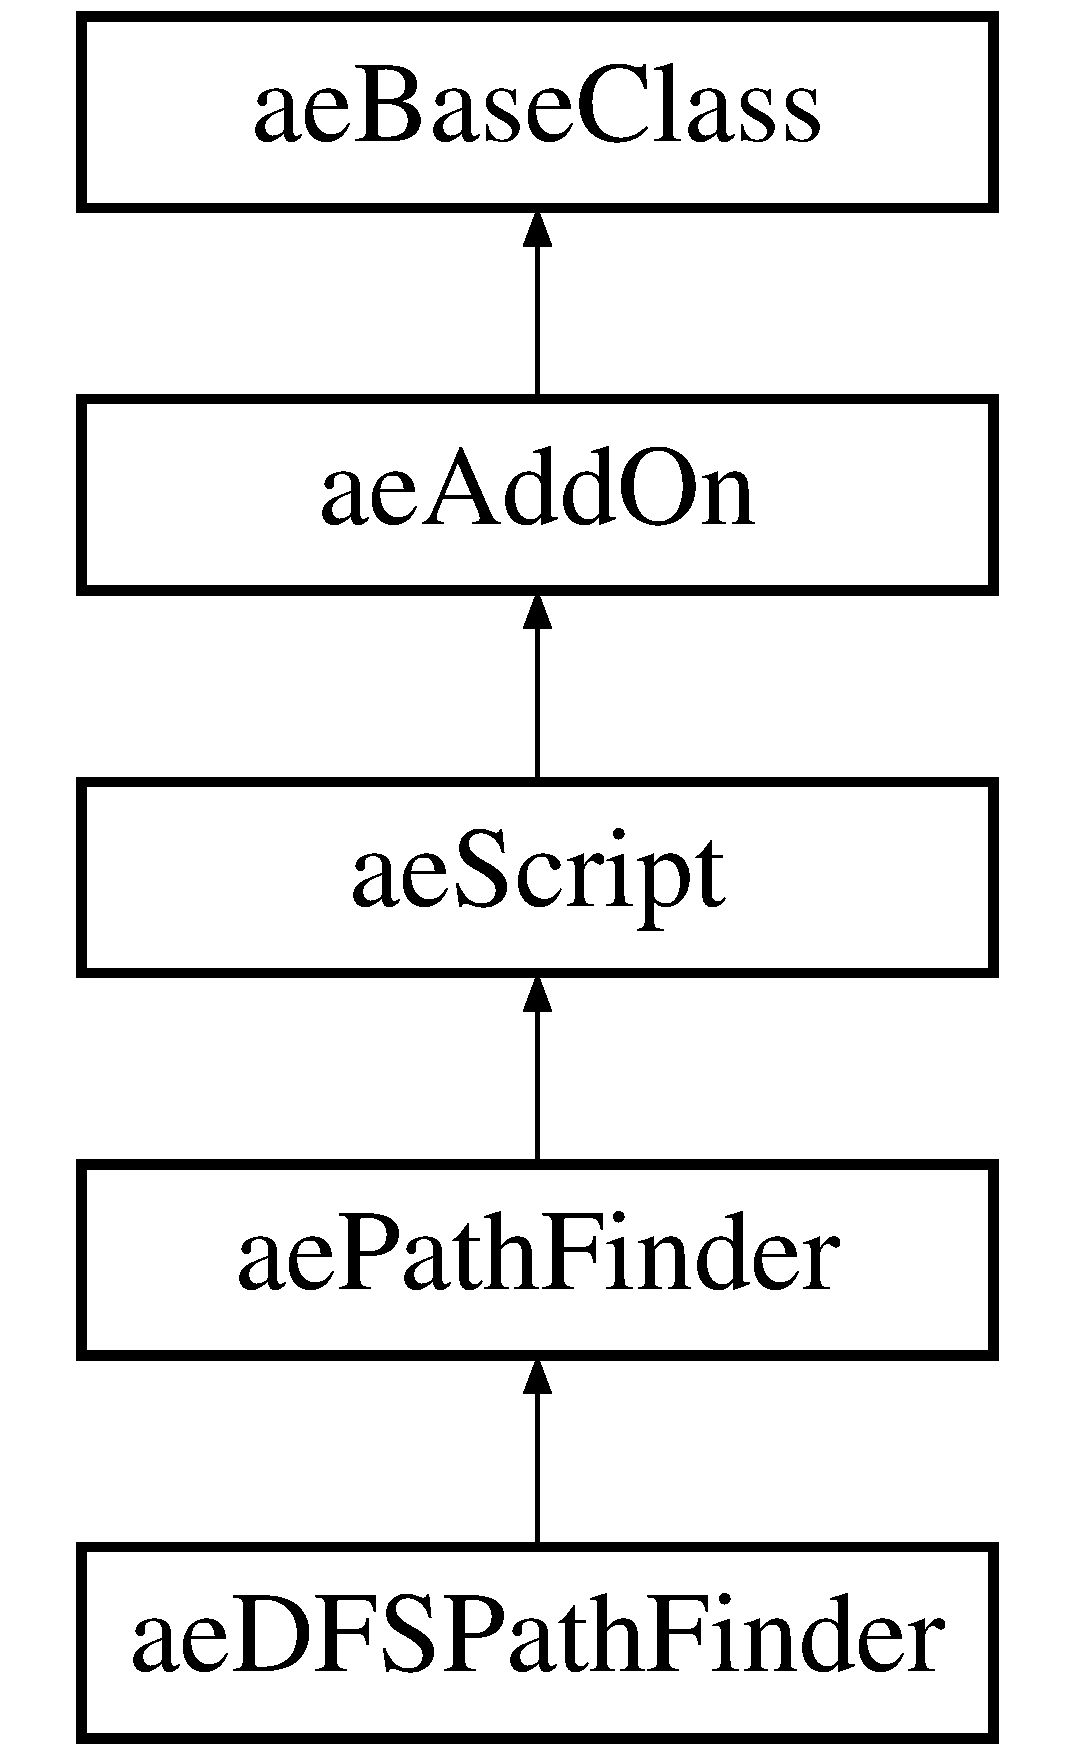
\includegraphics[height=5.000000cm]{classae_d_f_s_path_finder}
\end{center}
\end{figure}
\subsection*{Public Member Functions}
\begin{DoxyCompactItemize}
\item 
{\bfseries ae\+D\+F\+S\+Path\+Finder} (\hyperlink{classae_tiled_map}{ae\+Tiled\+Map} $\ast$p\+Map)\hypertarget{classae_d_f_s_path_finder_a34e76a7ed15b44cbd938888c2c80efb0}{}\label{classae_d_f_s_path_finder_a34e76a7ed15b44cbd938888c2c80efb0}

\item 
virtual int \hyperlink{classae_d_f_s_path_finder_a520c7725e3322b43fd7320da622c1b75}{Init} (\hyperlink{classae_base_class}{ae\+Base\+Class} $\ast$p\+Parent)
\begin{DoxyCompactList}\small\item\em Initializes with the given parent pointer. \end{DoxyCompactList}\item 
virtual void \hyperlink{classae_d_f_s_path_finder_a18f1efb48ab57e5e9eb94b29b8459430}{Destroy} ()\hypertarget{classae_d_f_s_path_finder_a18f1efb48ab57e5e9eb94b29b8459430}{}\label{classae_d_f_s_path_finder_a18f1efb48ab57e5e9eb94b29b8459430}

\begin{DoxyCompactList}\small\item\em Destroys this object. \end{DoxyCompactList}\item 
virtual void \hyperlink{classae_d_f_s_path_finder_a7751f27e031719afee45bfd29731b969}{Update} (float f\+Delta)
\begin{DoxyCompactList}\small\item\em Updates the given f\+Delta. \end{DoxyCompactList}\item 
virtual void \hyperlink{classae_d_f_s_path_finder_a2dc1c27f419be5b7a3e94c8be93aede6}{Render} (\hyperlink{classae_core_1_1ae_renderer}{ae\+Renderer} $\ast$p\+Renderer)
\begin{DoxyCompactList}\small\item\em Renders the given Renderer pointer. \end{DoxyCompactList}\item 
virtual void \hyperlink{classae_d_f_s_path_finder_a751a469a5e0177cf419a60563749bd6a}{Reset} ()\hypertarget{classae_d_f_s_path_finder_a751a469a5e0177cf419a60563749bd6a}{}\label{classae_d_f_s_path_finder_a751a469a5e0177cf419a60563749bd6a}

\begin{DoxyCompactList}\small\item\em Resets this object. \end{DoxyCompactList}\end{DoxyCompactItemize}
\subsection*{Protected Member Functions}
\begin{DoxyCompactItemize}
\item 
virtual void \hyperlink{classae_d_f_s_path_finder_a9a15c735ca42c68cb129641d79579be2}{Visit\+Grid\+Node} (\hyperlink{namespaceae_core_a862bc39eb87cfabca273f49e2a920129}{int32} x, \hyperlink{namespaceae_core_a862bc39eb87cfabca273f49e2a920129}{int32} y)
\begin{DoxyCompactList}\small\item\em Marks a node as visited. \end{DoxyCompactList}\item 
virtual void \hyperlink{classae_d_f_s_path_finder_a03ff9422ae609b83479783e8f1adf9aa}{Set\+Final\+Node} (\hyperlink{namespaceae_core_a862bc39eb87cfabca273f49e2a920129}{int32} x, \hyperlink{namespaceae_core_a862bc39eb87cfabca273f49e2a920129}{int32} y)
\begin{DoxyCompactList}\small\item\em Sets final node. \end{DoxyCompactList}\item 
virtual Walk\+State\+ID \hyperlink{classae_d_f_s_path_finder_a752e123b4e24cf7af2f11a3077ace616}{Give\+A\+Step} ()
\begin{DoxyCompactList}\small\item\em Give a step. \end{DoxyCompactList}\end{DoxyCompactItemize}
\subsection*{Additional Inherited Members}


\subsection{Member Function Documentation}
\index{ae\+D\+F\+S\+Path\+Finder@{ae\+D\+F\+S\+Path\+Finder}!Give\+A\+Step@{Give\+A\+Step}}
\index{Give\+A\+Step@{Give\+A\+Step}!ae\+D\+F\+S\+Path\+Finder@{ae\+D\+F\+S\+Path\+Finder}}
\subsubsection[{\texorpdfstring{Give\+A\+Step()}{GiveAStep()}}]{\setlength{\rightskip}{0pt plus 5cm}Walk\+State\+ID ae\+D\+F\+S\+Path\+Finder\+::\+Give\+A\+Step (
\begin{DoxyParamCaption}
{}
\end{DoxyParamCaption}
)\hspace{0.3cm}{\ttfamily [protected]}, {\ttfamily [virtual]}}\hypertarget{classae_d_f_s_path_finder_a752e123b4e24cf7af2f11a3077ace616}{}\label{classae_d_f_s_path_finder_a752e123b4e24cf7af2f11a3077ace616}


Give a step. 

\begin{DoxyReturn}{Returns}
A Walk\+State\+ID. 
\end{DoxyReturn}


Implements \hyperlink{classae_path_finder_a49332ee3be744cac1ece9ffd503ca218}{ae\+Path\+Finder}.

\index{ae\+D\+F\+S\+Path\+Finder@{ae\+D\+F\+S\+Path\+Finder}!Init@{Init}}
\index{Init@{Init}!ae\+D\+F\+S\+Path\+Finder@{ae\+D\+F\+S\+Path\+Finder}}
\subsubsection[{\texorpdfstring{Init(ae\+Base\+Class $\ast$p\+Parent)}{Init(aeBaseClass *pParent)}}]{\setlength{\rightskip}{0pt plus 5cm}int ae\+D\+F\+S\+Path\+Finder\+::\+Init (
\begin{DoxyParamCaption}
\item[{{\bf ae\+Base\+Class} $\ast$}]{p\+Parent}
\end{DoxyParamCaption}
)\hspace{0.3cm}{\ttfamily [virtual]}}\hypertarget{classae_d_f_s_path_finder_a520c7725e3322b43fd7320da622c1b75}{}\label{classae_d_f_s_path_finder_a520c7725e3322b43fd7320da622c1b75}


Initializes with the given parent pointer. 


\begin{DoxyParams}[1]{Parameters}
\mbox{\tt in,out}  & {\em p\+Parent} & If non-\/null, the parent.\\
\hline
\end{DoxyParams}
\begin{DoxyReturn}{Returns}
An int. 
\end{DoxyReturn}


Reimplemented from \hyperlink{classae_path_finder_a3395375f3de8f3f55d7b780ff6815806}{ae\+Path\+Finder}.

\index{ae\+D\+F\+S\+Path\+Finder@{ae\+D\+F\+S\+Path\+Finder}!Render@{Render}}
\index{Render@{Render}!ae\+D\+F\+S\+Path\+Finder@{ae\+D\+F\+S\+Path\+Finder}}
\subsubsection[{\texorpdfstring{Render(ae\+Renderer $\ast$p\+Renderer)}{Render(aeRenderer *pRenderer)}}]{\setlength{\rightskip}{0pt plus 5cm}void ae\+D\+F\+S\+Path\+Finder\+::\+Render (
\begin{DoxyParamCaption}
\item[{{\bf ae\+Renderer} $\ast$}]{p\+Renderer}
\end{DoxyParamCaption}
)\hspace{0.3cm}{\ttfamily [virtual]}}\hypertarget{classae_d_f_s_path_finder_a2dc1c27f419be5b7a3e94c8be93aede6}{}\label{classae_d_f_s_path_finder_a2dc1c27f419be5b7a3e94c8be93aede6}


Renders the given Renderer pointer. 


\begin{DoxyParams}[1]{Parameters}
\mbox{\tt in,out}  & {\em p\+Renderer} & If non-\/null, the renderer. \\
\hline
\end{DoxyParams}


Reimplemented from \hyperlink{classae_add_on_ab6bed56009b9c92df8ae017a27587dc3}{ae\+Add\+On}.

\index{ae\+D\+F\+S\+Path\+Finder@{ae\+D\+F\+S\+Path\+Finder}!Set\+Final\+Node@{Set\+Final\+Node}}
\index{Set\+Final\+Node@{Set\+Final\+Node}!ae\+D\+F\+S\+Path\+Finder@{ae\+D\+F\+S\+Path\+Finder}}
\subsubsection[{\texorpdfstring{Set\+Final\+Node(int32 x, int32 y)}{SetFinalNode(int32 x, int32 y)}}]{\setlength{\rightskip}{0pt plus 5cm}void ae\+D\+F\+S\+Path\+Finder\+::\+Set\+Final\+Node (
\begin{DoxyParamCaption}
\item[{{\bf int32}}]{x, }
\item[{{\bf int32}}]{y}
\end{DoxyParamCaption}
)\hspace{0.3cm}{\ttfamily [protected]}, {\ttfamily [virtual]}}\hypertarget{classae_d_f_s_path_finder_a03ff9422ae609b83479783e8f1adf9aa}{}\label{classae_d_f_s_path_finder_a03ff9422ae609b83479783e8f1adf9aa}


Sets final node. 


\begin{DoxyParams}{Parameters}
{\em x} & The x coordinate. \\
\hline
{\em y} & The y coordinate. \\
\hline
\end{DoxyParams}
\index{ae\+D\+F\+S\+Path\+Finder@{ae\+D\+F\+S\+Path\+Finder}!Update@{Update}}
\index{Update@{Update}!ae\+D\+F\+S\+Path\+Finder@{ae\+D\+F\+S\+Path\+Finder}}
\subsubsection[{\texorpdfstring{Update(float f\+Delta)}{Update(float fDelta)}}]{\setlength{\rightskip}{0pt plus 5cm}void ae\+D\+F\+S\+Path\+Finder\+::\+Update (
\begin{DoxyParamCaption}
\item[{float}]{f\+Delta}
\end{DoxyParamCaption}
)\hspace{0.3cm}{\ttfamily [virtual]}}\hypertarget{classae_d_f_s_path_finder_a7751f27e031719afee45bfd29731b969}{}\label{classae_d_f_s_path_finder_a7751f27e031719afee45bfd29731b969}


Updates the given f\+Delta. 


\begin{DoxyParams}{Parameters}
{\em f\+Delta} & The delta. \\
\hline
\end{DoxyParams}


Implements \hyperlink{classae_add_on_a51caa4b8680206495ea671e71991e231}{ae\+Add\+On}.

\index{ae\+D\+F\+S\+Path\+Finder@{ae\+D\+F\+S\+Path\+Finder}!Visit\+Grid\+Node@{Visit\+Grid\+Node}}
\index{Visit\+Grid\+Node@{Visit\+Grid\+Node}!ae\+D\+F\+S\+Path\+Finder@{ae\+D\+F\+S\+Path\+Finder}}
\subsubsection[{\texorpdfstring{Visit\+Grid\+Node(int32 x, int32 y)}{VisitGridNode(int32 x, int32 y)}}]{\setlength{\rightskip}{0pt plus 5cm}void ae\+D\+F\+S\+Path\+Finder\+::\+Visit\+Grid\+Node (
\begin{DoxyParamCaption}
\item[{{\bf int32}}]{x, }
\item[{{\bf int32}}]{y}
\end{DoxyParamCaption}
)\hspace{0.3cm}{\ttfamily [protected]}, {\ttfamily [virtual]}}\hypertarget{classae_d_f_s_path_finder_a9a15c735ca42c68cb129641d79579be2}{}\label{classae_d_f_s_path_finder_a9a15c735ca42c68cb129641d79579be2}


Marks a node as visited. 


\begin{DoxyParams}{Parameters}
{\em x} & The x coordinate. \\
\hline
{\em y} & The y coordinate. \\
\hline
\end{DoxyParams}


Implements \hyperlink{classae_path_finder_a4ccfa19ff344b9f4827dbeab18c4efab}{ae\+Path\+Finder}.



The documentation for this class was generated from the following files\+:\begin{DoxyCompactItemize}
\item 
C\+:/\+Users/\+Alvaro Estrada/\+Documents/\+Visual Studio 2015/\+Projects/\+R\+T\+S\+\_\+\+A\+E/\+R\+T\+S\+\_\+\+A\+E/\+Game/Depth\+First\+Search.\+h\item 
C\+:/\+Users/\+Alvaro Estrada/\+Documents/\+Visual Studio 2015/\+Projects/\+R\+T\+S\+\_\+\+A\+E/\+R\+T\+S\+\_\+\+A\+E/\+Game/Depth\+First\+Search.\+cpp\end{DoxyCompactItemize}

\hypertarget{classae_dijkstra_path_finder}{}\section{ae\+Dijkstra\+Path\+Finder Class Reference}
\label{classae_dijkstra_path_finder}\index{ae\+Dijkstra\+Path\+Finder@{ae\+Dijkstra\+Path\+Finder}}
Inheritance diagram for ae\+Dijkstra\+Path\+Finder\+:\begin{figure}[H]
\begin{center}
\leavevmode
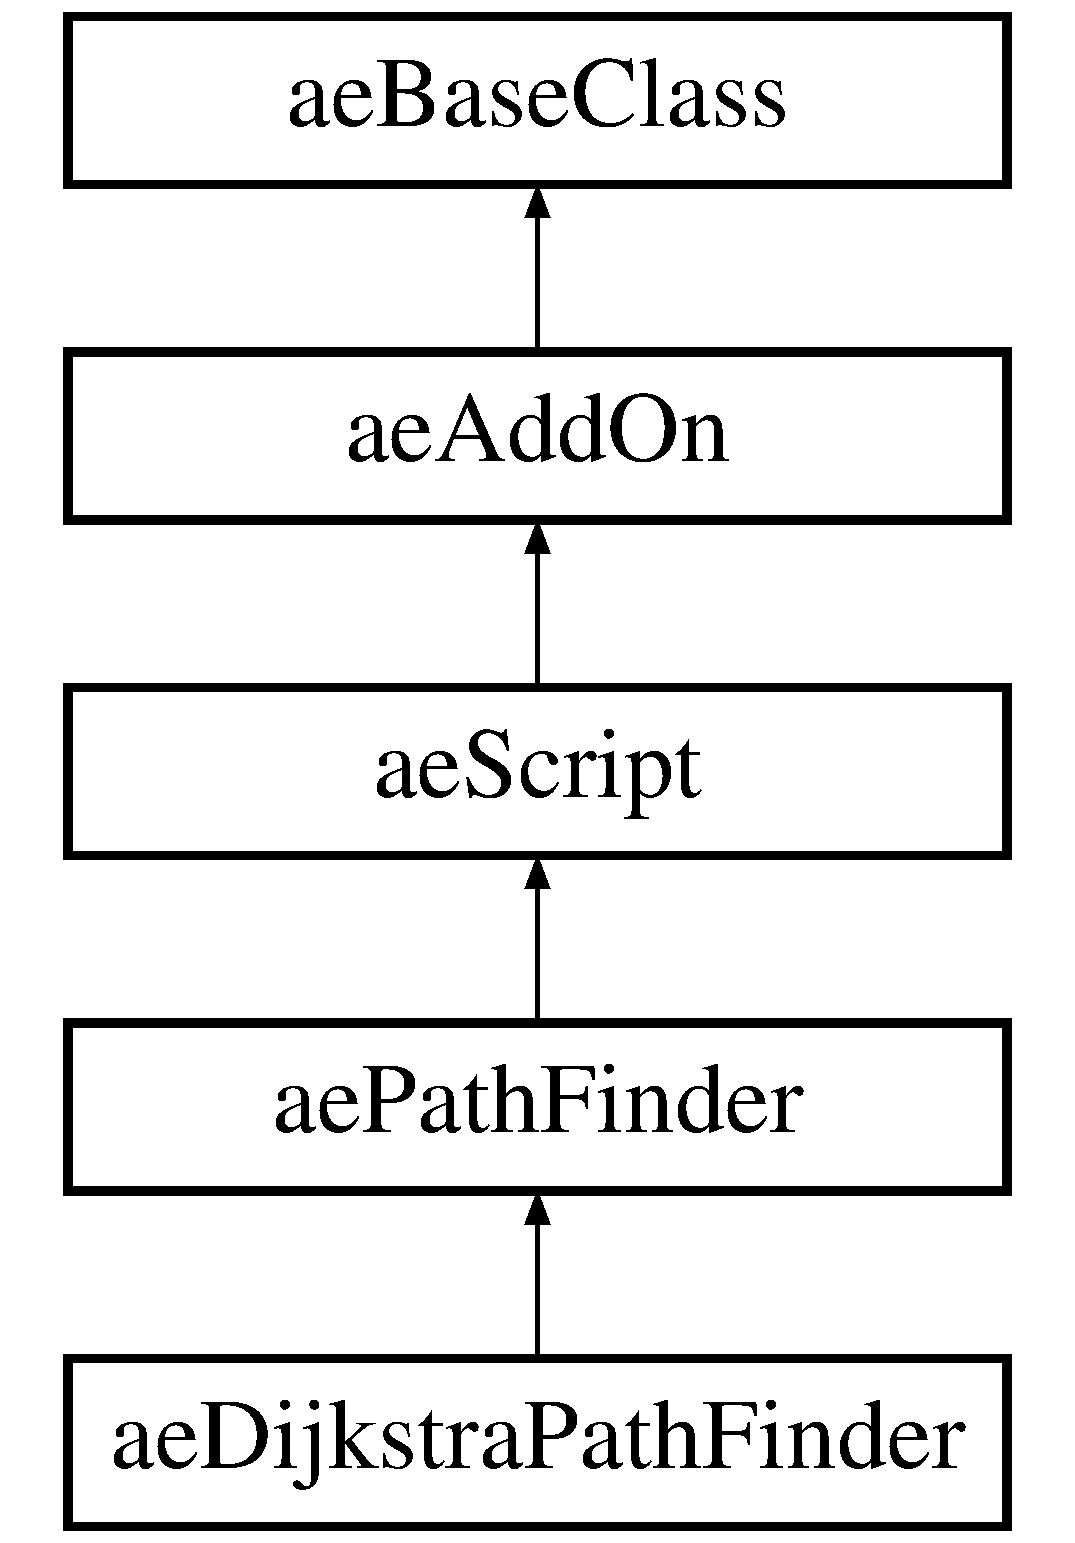
\includegraphics[height=5.000000cm]{classae_dijkstra_path_finder}
\end{center}
\end{figure}
\subsection*{Classes}
\begin{DoxyCompactItemize}
\item 
struct \hyperlink{structae_dijkstra_path_finder_1_1_node_dist}{Node\+Dist}
\item 
struct \hyperlink{structae_dijkstra_path_finder_1_1_tile_compare}{Tile\+Compare}
\end{DoxyCompactItemize}
\subsection*{Public Member Functions}
\begin{DoxyCompactItemize}
\item 
{\bfseries ae\+Dijkstra\+Path\+Finder} (\hyperlink{classae_tiled_map}{ae\+Tiled\+Map} $\ast$p\+Map)\hypertarget{classae_dijkstra_path_finder_acc5e17fae2b26a51e2b5017cc79ee776}{}\label{classae_dijkstra_path_finder_acc5e17fae2b26a51e2b5017cc79ee776}

\item 
virtual int \hyperlink{classae_dijkstra_path_finder_a0cc9454fad1387bba68f879afb1f2526}{Init} (\hyperlink{classae_base_class}{ae\+Base\+Class} $\ast$p\+Parent)
\begin{DoxyCompactList}\small\item\em Initializes with the given parent pointer. \end{DoxyCompactList}\item 
virtual void \hyperlink{classae_dijkstra_path_finder_ad9639e3ff07de514f28124f7318ebe33}{Destroy} ()\hypertarget{classae_dijkstra_path_finder_ad9639e3ff07de514f28124f7318ebe33}{}\label{classae_dijkstra_path_finder_ad9639e3ff07de514f28124f7318ebe33}

\begin{DoxyCompactList}\small\item\em Destroys this object. \end{DoxyCompactList}\item 
virtual void \hyperlink{classae_dijkstra_path_finder_a400f2f0645f9939bc11c140b3e6cf3d8}{Update} (float f\+Delta)
\begin{DoxyCompactList}\small\item\em Updates the given f\+Delta. \end{DoxyCompactList}\item 
virtual void \hyperlink{classae_dijkstra_path_finder_a75779c09b89c1262cc216f081763927d}{Render} (\hyperlink{classae_core_1_1ae_renderer}{ae\+Renderer} $\ast$p\+Renderer)
\begin{DoxyCompactList}\small\item\em Renders the given Renderer pointer. \end{DoxyCompactList}\item 
virtual void \hyperlink{classae_dijkstra_path_finder_a19def2693faf239d6c8cf36a573d3ab9}{Reset} ()\hypertarget{classae_dijkstra_path_finder_a19def2693faf239d6c8cf36a573d3ab9}{}\label{classae_dijkstra_path_finder_a19def2693faf239d6c8cf36a573d3ab9}

\begin{DoxyCompactList}\small\item\em Resets this object. \end{DoxyCompactList}\end{DoxyCompactItemize}
\subsection*{Protected Member Functions}
\begin{DoxyCompactItemize}
\item 
virtual void \hyperlink{classae_dijkstra_path_finder_a06cbc7f3215eb10e66bffc69cd051dae}{Visit\+Grid\+Node} (\hyperlink{namespaceae_core_a862bc39eb87cfabca273f49e2a920129}{int32} x, \hyperlink{namespaceae_core_a862bc39eb87cfabca273f49e2a920129}{int32} y)
\begin{DoxyCompactList}\small\item\em Marks a node as visited. \end{DoxyCompactList}\item 
virtual Walk\+State\+ID \hyperlink{classae_dijkstra_path_finder_a14ca862aa79790d77d1df8d54f99aa39}{Give\+A\+Step} ()
\begin{DoxyCompactList}\small\item\em Give a step. \end{DoxyCompactList}\end{DoxyCompactItemize}
\subsection*{Additional Inherited Members}


\subsection{Member Function Documentation}
\index{ae\+Dijkstra\+Path\+Finder@{ae\+Dijkstra\+Path\+Finder}!Give\+A\+Step@{Give\+A\+Step}}
\index{Give\+A\+Step@{Give\+A\+Step}!ae\+Dijkstra\+Path\+Finder@{ae\+Dijkstra\+Path\+Finder}}
\subsubsection[{\texorpdfstring{Give\+A\+Step()}{GiveAStep()}}]{\setlength{\rightskip}{0pt plus 5cm}Walk\+State\+ID ae\+Dijkstra\+Path\+Finder\+::\+Give\+A\+Step (
\begin{DoxyParamCaption}
{}
\end{DoxyParamCaption}
)\hspace{0.3cm}{\ttfamily [protected]}, {\ttfamily [virtual]}}\hypertarget{classae_dijkstra_path_finder_a14ca862aa79790d77d1df8d54f99aa39}{}\label{classae_dijkstra_path_finder_a14ca862aa79790d77d1df8d54f99aa39}


Give a step. 

\begin{DoxyReturn}{Returns}
A Walk\+State\+ID. 
\end{DoxyReturn}


Implements \hyperlink{classae_path_finder_a49332ee3be744cac1ece9ffd503ca218}{ae\+Path\+Finder}.

\index{ae\+Dijkstra\+Path\+Finder@{ae\+Dijkstra\+Path\+Finder}!Init@{Init}}
\index{Init@{Init}!ae\+Dijkstra\+Path\+Finder@{ae\+Dijkstra\+Path\+Finder}}
\subsubsection[{\texorpdfstring{Init(ae\+Base\+Class $\ast$p\+Parent)}{Init(aeBaseClass *pParent)}}]{\setlength{\rightskip}{0pt plus 5cm}int ae\+Dijkstra\+Path\+Finder\+::\+Init (
\begin{DoxyParamCaption}
\item[{{\bf ae\+Base\+Class} $\ast$}]{p\+Parent}
\end{DoxyParamCaption}
)\hspace{0.3cm}{\ttfamily [virtual]}}\hypertarget{classae_dijkstra_path_finder_a0cc9454fad1387bba68f879afb1f2526}{}\label{classae_dijkstra_path_finder_a0cc9454fad1387bba68f879afb1f2526}


Initializes with the given parent pointer. 


\begin{DoxyParams}[1]{Parameters}
\mbox{\tt in,out}  & {\em p\+Parent} & If non-\/null, the parent.\\
\hline
\end{DoxyParams}
\begin{DoxyReturn}{Returns}
An int. 
\end{DoxyReturn}


Reimplemented from \hyperlink{classae_path_finder_a3395375f3de8f3f55d7b780ff6815806}{ae\+Path\+Finder}.

\index{ae\+Dijkstra\+Path\+Finder@{ae\+Dijkstra\+Path\+Finder}!Render@{Render}}
\index{Render@{Render}!ae\+Dijkstra\+Path\+Finder@{ae\+Dijkstra\+Path\+Finder}}
\subsubsection[{\texorpdfstring{Render(ae\+Renderer $\ast$p\+Renderer)}{Render(aeRenderer *pRenderer)}}]{\setlength{\rightskip}{0pt plus 5cm}void ae\+Dijkstra\+Path\+Finder\+::\+Render (
\begin{DoxyParamCaption}
\item[{{\bf ae\+Renderer} $\ast$}]{p\+Renderer}
\end{DoxyParamCaption}
)\hspace{0.3cm}{\ttfamily [virtual]}}\hypertarget{classae_dijkstra_path_finder_a75779c09b89c1262cc216f081763927d}{}\label{classae_dijkstra_path_finder_a75779c09b89c1262cc216f081763927d}


Renders the given Renderer pointer. 


\begin{DoxyParams}[1]{Parameters}
\mbox{\tt in,out}  & {\em p\+Renderer} & If non-\/null, the renderer. \\
\hline
\end{DoxyParams}


Reimplemented from \hyperlink{classae_add_on_ab6bed56009b9c92df8ae017a27587dc3}{ae\+Add\+On}.

\index{ae\+Dijkstra\+Path\+Finder@{ae\+Dijkstra\+Path\+Finder}!Update@{Update}}
\index{Update@{Update}!ae\+Dijkstra\+Path\+Finder@{ae\+Dijkstra\+Path\+Finder}}
\subsubsection[{\texorpdfstring{Update(float f\+Delta)}{Update(float fDelta)}}]{\setlength{\rightskip}{0pt plus 5cm}void ae\+Dijkstra\+Path\+Finder\+::\+Update (
\begin{DoxyParamCaption}
\item[{float}]{f\+Delta}
\end{DoxyParamCaption}
)\hspace{0.3cm}{\ttfamily [virtual]}}\hypertarget{classae_dijkstra_path_finder_a400f2f0645f9939bc11c140b3e6cf3d8}{}\label{classae_dijkstra_path_finder_a400f2f0645f9939bc11c140b3e6cf3d8}


Updates the given f\+Delta. 


\begin{DoxyParams}{Parameters}
{\em f\+Delta} & The delta. \\
\hline
\end{DoxyParams}


Implements \hyperlink{classae_add_on_a51caa4b8680206495ea671e71991e231}{ae\+Add\+On}.

\index{ae\+Dijkstra\+Path\+Finder@{ae\+Dijkstra\+Path\+Finder}!Visit\+Grid\+Node@{Visit\+Grid\+Node}}
\index{Visit\+Grid\+Node@{Visit\+Grid\+Node}!ae\+Dijkstra\+Path\+Finder@{ae\+Dijkstra\+Path\+Finder}}
\subsubsection[{\texorpdfstring{Visit\+Grid\+Node(int32 x, int32 y)}{VisitGridNode(int32 x, int32 y)}}]{\setlength{\rightskip}{0pt plus 5cm}void ae\+Dijkstra\+Path\+Finder\+::\+Visit\+Grid\+Node (
\begin{DoxyParamCaption}
\item[{{\bf int32}}]{x, }
\item[{{\bf int32}}]{y}
\end{DoxyParamCaption}
)\hspace{0.3cm}{\ttfamily [protected]}, {\ttfamily [virtual]}}\hypertarget{classae_dijkstra_path_finder_a06cbc7f3215eb10e66bffc69cd051dae}{}\label{classae_dijkstra_path_finder_a06cbc7f3215eb10e66bffc69cd051dae}


Marks a node as visited. 


\begin{DoxyParams}{Parameters}
{\em x} & The x coordinate. \\
\hline
{\em y} & The y coordinate. \\
\hline
\end{DoxyParams}


Implements \hyperlink{classae_path_finder_a4ccfa19ff344b9f4827dbeab18c4efab}{ae\+Path\+Finder}.



The documentation for this class was generated from the following files\+:\begin{DoxyCompactItemize}
\item 
C\+:/\+Users/\+Alvaro Estrada/\+Documents/\+Visual Studio 2015/\+Projects/\+R\+T\+S\+\_\+\+A\+E/\+R\+T\+S\+\_\+\+A\+E/\+Game/Dijkstra.\+h\item 
C\+:/\+Users/\+Alvaro Estrada/\+Documents/\+Visual Studio 2015/\+Projects/\+R\+T\+S\+\_\+\+A\+E/\+R\+T\+S\+\_\+\+A\+E/\+Game/Dijkstra.\+cpp\end{DoxyCompactItemize}

\hypertarget{structae_core_1_1ae_event}{}\section{ae\+Core\+:\+:ae\+Event Struct Reference}
\label{structae_core_1_1ae_event}\index{ae\+Core\+::ae\+Event@{ae\+Core\+::ae\+Event}}


An event message.  




{\ttfamily \#include $<$Events\+System.\+h$>$}

Inheritance diagram for ae\+Core\+:\+:ae\+Event\+:\begin{figure}[H]
\begin{center}
\leavevmode
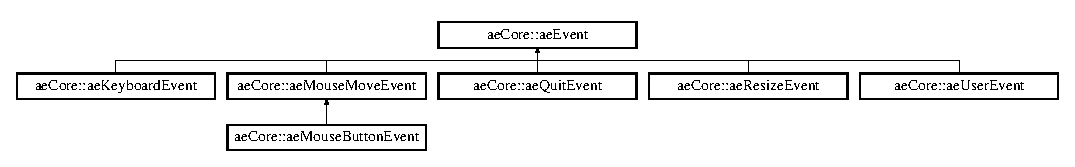
\includegraphics[height=1.796791cm]{structae_core_1_1ae_event}
\end{center}
\end{figure}
\subsection*{Public Attributes}
\begin{DoxyCompactItemize}
\item 
\hyperlink{namespaceae_core_aa13093dc911869e5b24942552898f01f}{uint8} {\bfseries Type}\hypertarget{structae_core_1_1ae_event_ad3204f8b2c4098c90b8f773b85368e80}{}\label{structae_core_1_1ae_event_ad3204f8b2c4098c90b8f773b85368e80}

\item 
\hyperlink{namespaceae_core_aa13093dc911869e5b24942552898f01f}{uint8} {\bfseries Priority}\hypertarget{structae_core_1_1ae_event_ac8be00cb6fbc2e43485b4e95e177f670}{}\label{structae_core_1_1ae_event_ac8be00cb6fbc2e43485b4e95e177f670}

\end{DoxyCompactItemize}


\subsection{Detailed Description}
An event message. 

The documentation for this struct was generated from the following file\+:\begin{DoxyCompactItemize}
\item 
C\+:/\+Users/\+Alvaro Estrada/\+Documents/\+Visual Studio 2015/\+Projects/\+R\+T\+S\+\_\+\+A\+E/ae\+Core/\+Event\+System/Events\+System.\+h\end{DoxyCompactItemize}

\hypertarget{structae_core_1_1ae_events_handler}{}\section{ae\+Core\+:\+:ae\+Events\+Handler Struct Reference}
\label{structae_core_1_1ae_events_handler}\index{ae\+Core\+::ae\+Events\+Handler@{ae\+Core\+::ae\+Events\+Handler}}


This class stores all the events in a vector, and stores temporal events a queue for in-\/n-\/out communication.  




{\ttfamily \#include $<$Events\+System.\+h$>$}

\subsection*{Classes}
\begin{DoxyCompactItemize}
\item 
struct \hyperlink{structae_core_1_1ae_events_handler_1_1_event_compare}{Event\+Compare}
\end{DoxyCompactItemize}
\subsection*{Public Attributes}
\begin{DoxyCompactItemize}
\item 
std\+::priority\+\_\+queue$<$ \hyperlink{structae_core_1_1ae_event}{ae\+Event} $\ast$, std\+::vector$<$ \hyperlink{structae_core_1_1ae_event}{ae\+Event} $\ast$ $>$, \hyperlink{structae_core_1_1ae_events_handler_1_1_event_compare}{Event\+Compare} $>$ {\bfseries m\+\_\+a\+Message\+Pile}\hypertarget{structae_core_1_1ae_events_handler_a34477930b3369b9ee1977f548575a512}{}\label{structae_core_1_1ae_events_handler_a34477930b3369b9ee1977f548575a512}

\item 
std\+::vector$<$ \hyperlink{structae_core_1_1ae_event}{ae\+Event} $\ast$ $>$ {\bfseries m\+\_\+a\+History}\hypertarget{structae_core_1_1ae_events_handler_aaa6d8d9debd62ad2d8b905d25d8e7c14}{}\label{structae_core_1_1ae_events_handler_aaa6d8d9debd62ad2d8b905d25d8e7c14}

\end{DoxyCompactItemize}


\subsection{Detailed Description}
This class stores all the events in a vector, and stores temporal events a queue for in-\/n-\/out communication. 

The documentation for this struct was generated from the following files\+:\begin{DoxyCompactItemize}
\item 
C\+:/\+Users/\+Alvaro Estrada/\+Documents/\+Visual Studio 2015/\+Projects/\+R\+T\+S\+\_\+\+A\+E/ae\+Core/\+Event\+System/Events\+System.\+h\item 
C\+:/\+Users/\+Alvaro Estrada/\+Documents/\+Visual Studio 2015/\+Projects/\+R\+T\+S\+\_\+\+A\+E/ae\+Core/\+Event\+System/Events\+System.\+cpp\end{DoxyCompactItemize}

\hypertarget{classae_core_1_1ae_font}{}\section{ae\+Core\+:\+:ae\+Font Class Reference}
\label{classae_core_1_1ae_font}\index{ae\+Core\+::ae\+Font@{ae\+Core\+::ae\+Font}}


An ae font.  




{\ttfamily \#include $<$Sprite.\+h$>$}

\subsection*{Public Member Functions}
\begin{DoxyCompactItemize}
\item 
{\bfseries ae\+Font} (\hyperlink{namespaceae_core_ad6f85aacc0d1fdd85e458e2413e60010}{ae\+String} \&File\+Path, \hyperlink{namespaceae_core_ad6f85aacc0d1fdd85e458e2413e60010}{ae\+String} \&Name, int Size)\hypertarget{classae_core_1_1ae_font_ae393e09d36bae786208a0abbdc6936c7}{}\label{classae_core_1_1ae_font_ae393e09d36bae786208a0abbdc6936c7}

\item 
int {\bfseries Init} (\hyperlink{namespaceae_core_ad6f85aacc0d1fdd85e458e2413e60010}{ae\+String} \&File\+Path, \hyperlink{namespaceae_core_ad6f85aacc0d1fdd85e458e2413e60010}{ae\+String} \&Name, int Size)\hypertarget{classae_core_1_1ae_font_ad73c7edd18dd4148b628c2ed3933fe90}{}\label{classae_core_1_1ae_font_ad73c7edd18dd4148b628c2ed3933fe90}

\item 
void {\bfseries Destroy} ()\hypertarget{classae_core_1_1ae_font_a024a5c7aaef22cb5523a48082b80d71b}{}\label{classae_core_1_1ae_font_a024a5c7aaef22cb5523a48082b80d71b}

\item 
int {\bfseries Get\+Size} ()\hypertarget{classae_core_1_1ae_font_a2c593d71a9c27dde4e76f7d0064ba66c}{}\label{classae_core_1_1ae_font_a2c593d71a9c27dde4e76f7d0064ba66c}

\item 
\hyperlink{namespaceae_core_ad6f85aacc0d1fdd85e458e2413e60010}{ae\+String} \& {\bfseries Get\+Name} ()\hypertarget{classae_core_1_1ae_font_a656058109d674aec5c9524e8455936b0}{}\label{classae_core_1_1ae_font_a656058109d674aec5c9524e8455936b0}

\item 
void {\bfseries Change\+Size} (int Size)\hypertarget{classae_core_1_1ae_font_a2cf79cfabad6234278f87dd09649907d}{}\label{classae_core_1_1ae_font_a2cf79cfabad6234278f87dd09649907d}

\end{DoxyCompactItemize}
\subsection*{Friends}
\begin{DoxyCompactItemize}
\item 
class {\bfseries ae\+Sprite}\hypertarget{classae_core_1_1ae_font_a450e94d8bab3fa5d26d3663ba55b8ba3}{}\label{classae_core_1_1ae_font_a450e94d8bab3fa5d26d3663ba55b8ba3}

\end{DoxyCompactItemize}


\subsection{Detailed Description}
An ae font. 

The documentation for this class was generated from the following files\+:\begin{DoxyCompactItemize}
\item 
C\+:/\+Users/\+Alvaro Estrada/\+Documents/\+Visual Studio 2015/\+Projects/\+R\+T\+S\+\_\+\+A\+E/ae\+Core/\+Graphics/\hyperlink{_sprite_8h}{Sprite.\+h}\item 
C\+:/\+Users/\+Alvaro Estrada/\+Documents/\+Visual Studio 2015/\+Projects/\+R\+T\+S\+\_\+\+A\+E/ae\+Core/\+Graphics/\hyperlink{_sprite_8cpp}{Sprite.\+cpp}\end{DoxyCompactItemize}

\hypertarget{classae_game_object}{}\section{ae\+Game\+Object Class Reference}
\label{classae_game_object}\index{ae\+Game\+Object@{ae\+Game\+Object}}


A game object.  




{\ttfamily \#include $<$Game\+Object.\+h$>$}

Inheritance diagram for ae\+Game\+Object\+:\begin{figure}[H]
\begin{center}
\leavevmode
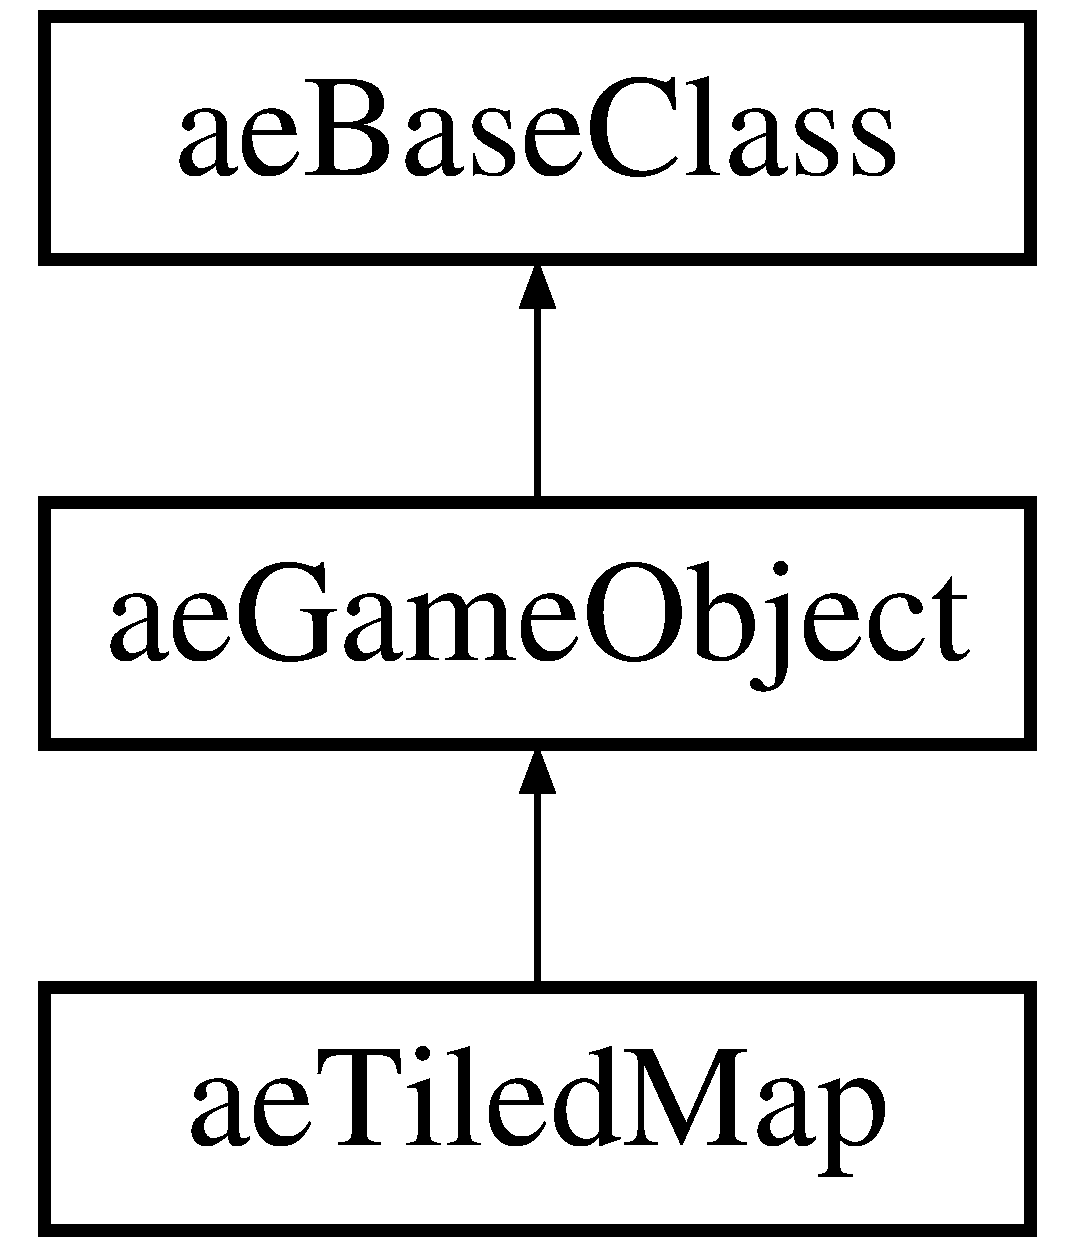
\includegraphics[height=3.000000cm]{classae_game_object}
\end{center}
\end{figure}
\subsection*{Public Member Functions}
\begin{DoxyCompactItemize}
\item 
virtual int \hyperlink{classae_game_object_ab4e04a67ee1f5d7a23966792577534e6}{Init} ()
\begin{DoxyCompactList}\small\item\em Initializes this object, returns 0 in case of a correct initialization. \end{DoxyCompactList}\item 
virtual void \hyperlink{classae_game_object_ab43b31f1179579df835873e60ae84f32}{Update} (float f\+Delta)
\begin{DoxyCompactList}\small\item\em Updates given f\+Delta. \end{DoxyCompactList}\item 
virtual void \hyperlink{classae_game_object_ae2ab1d6a65f6008766faa8295affc9fe}{Render} (\hyperlink{classae_core_1_1ae_renderer}{ae\+Renderer} $\ast$p\+Renderer)
\begin{DoxyCompactList}\small\item\em Renders this object given its given renderer pointer. \end{DoxyCompactList}\item 
virtual void \hyperlink{classae_game_object_af7faadfae20c3d83d521b7e1b4e4b06b}{Destroy} ()\hypertarget{classae_game_object_af7faadfae20c3d83d521b7e1b4e4b06b}{}\label{classae_game_object_af7faadfae20c3d83d521b7e1b4e4b06b}

\begin{DoxyCompactList}\small\item\em Destroys this object. \end{DoxyCompactList}\end{DoxyCompactItemize}
\subsection*{Public Attributes}
\begin{DoxyCompactItemize}
\item 
\hyperlink{structae_transform}{ae\+Transform} {\bfseries Transform}\hypertarget{classae_game_object_a89138ab3368a2fc33260fbdb38cca3f1}{}\label{classae_game_object_a89138ab3368a2fc33260fbdb38cca3f1}

\item 
ae\+String {\bfseries Name}\hypertarget{classae_game_object_a4b63043d812d56ae14101029c524642d}{}\label{classae_game_object_a4b63043d812d56ae14101029c524642d}

\item 
ae\+String {\bfseries Tag}\hypertarget{classae_game_object_a255311c9e0d138c0407736f8108386c3}{}\label{classae_game_object_a255311c9e0d138c0407736f8108386c3}

\item 
\hyperlink{_add_on_8h_a0f4072611b509766afe7bb36d570ac80}{ae\+Add\+Ons} {\bfseries Add\+Ons}\hypertarget{classae_game_object_a843f81854501b0b04f7777675f195db9}{}\label{classae_game_object_a843f81854501b0b04f7777675f195db9}

\item 
ae\+Children {\bfseries Children}\hypertarget{classae_game_object_ad0b7749e7572798c319b9be4ffac757d}{}\label{classae_game_object_ad0b7749e7572798c319b9be4ffac757d}

\end{DoxyCompactItemize}
\subsection*{Additional Inherited Members}


\subsection{Detailed Description}
A game object. 

\subsection{Member Function Documentation}
\index{ae\+Game\+Object@{ae\+Game\+Object}!Init@{Init}}
\index{Init@{Init}!ae\+Game\+Object@{ae\+Game\+Object}}
\subsubsection[{\texorpdfstring{Init()}{Init()}}]{\setlength{\rightskip}{0pt plus 5cm}int ae\+Game\+Object\+::\+Init (
\begin{DoxyParamCaption}
{}
\end{DoxyParamCaption}
)\hspace{0.3cm}{\ttfamily [virtual]}}\hypertarget{classae_game_object_ab4e04a67ee1f5d7a23966792577534e6}{}\label{classae_game_object_ab4e04a67ee1f5d7a23966792577534e6}


Initializes this object, returns 0 in case of a correct initialization. 

\begin{DoxyReturn}{Returns}
An int. 
\end{DoxyReturn}
\index{ae\+Game\+Object@{ae\+Game\+Object}!Render@{Render}}
\index{Render@{Render}!ae\+Game\+Object@{ae\+Game\+Object}}
\subsubsection[{\texorpdfstring{Render(ae\+Renderer $\ast$p\+Renderer)}{Render(aeRenderer *pRenderer)}}]{\setlength{\rightskip}{0pt plus 5cm}void ae\+Game\+Object\+::\+Render (
\begin{DoxyParamCaption}
\item[{{\bf ae\+Renderer} $\ast$}]{p\+Renderer}
\end{DoxyParamCaption}
)\hspace{0.3cm}{\ttfamily [virtual]}}\hypertarget{classae_game_object_ae2ab1d6a65f6008766faa8295affc9fe}{}\label{classae_game_object_ae2ab1d6a65f6008766faa8295affc9fe}


Renders this object given its given renderer pointer. 


\begin{DoxyParams}[1]{Parameters}
\mbox{\tt in,out}  & {\em p\+Renderer} & If non-\/null, the renderer. \\
\hline
\end{DoxyParams}


Reimplemented in \hyperlink{classae_tiled_map_a3f0816ebe094c6a1308524936d6c926e}{ae\+Tiled\+Map}.

\index{ae\+Game\+Object@{ae\+Game\+Object}!Update@{Update}}
\index{Update@{Update}!ae\+Game\+Object@{ae\+Game\+Object}}
\subsubsection[{\texorpdfstring{Update(float f\+Delta)}{Update(float fDelta)}}]{\setlength{\rightskip}{0pt plus 5cm}void ae\+Game\+Object\+::\+Update (
\begin{DoxyParamCaption}
\item[{float}]{f\+Delta}
\end{DoxyParamCaption}
)\hspace{0.3cm}{\ttfamily [virtual]}}\hypertarget{classae_game_object_ab43b31f1179579df835873e60ae84f32}{}\label{classae_game_object_ab43b31f1179579df835873e60ae84f32}


Updates given f\+Delta. 


\begin{DoxyParams}{Parameters}
{\em f\+Delta} & The delta. \\
\hline
\end{DoxyParams}


Reimplemented in \hyperlink{classae_tiled_map_a96e6f64deda9d9d02fef3cd173e900a8}{ae\+Tiled\+Map}.



The documentation for this class was generated from the following files\+:\begin{DoxyCompactItemize}
\item 
C\+:/\+Users/\+Alvaro Estrada/\+Documents/\+Visual Studio 2015/\+Projects/\+R\+T\+S\+\_\+\+A\+E/\+R\+T\+S\+\_\+\+A\+E/\+Game/Game\+Object.\+h\item 
C\+:/\+Users/\+Alvaro Estrada/\+Documents/\+Visual Studio 2015/\+Projects/\+R\+T\+S\+\_\+\+A\+E/\+R\+T\+S\+\_\+\+A\+E/\+Game/Game\+Object.\+cpp\end{DoxyCompactItemize}

\hypertarget{classae_g_u_i}{}\section{ae\+G\+UI Class Reference}
\label{classae_g_u_i}\index{ae\+G\+UI@{ae\+G\+UI}}
Inheritance diagram for ae\+G\+UI\+:\begin{figure}[H]
\begin{center}
\leavevmode
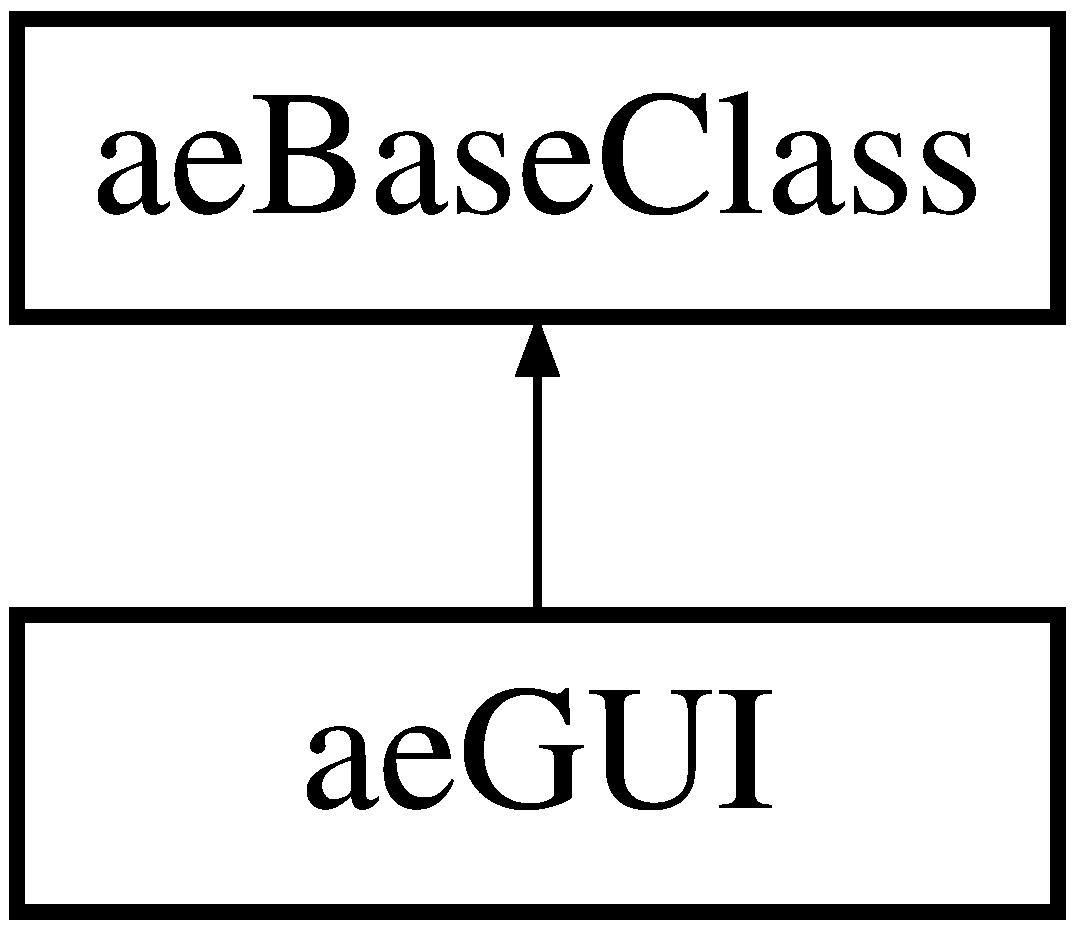
\includegraphics[height=2.000000cm]{classae_g_u_i}
\end{center}
\end{figure}
\subsection*{Public Member Functions}
\begin{DoxyCompactItemize}
\item 
int {\bfseries Init} (\hyperlink{namespaceae_core_ad6f85aacc0d1fdd85e458e2413e60010}{ae\+String} \&psz\+Bin\+File\+Path, \hyperlink{structae_core_1_1ae_rect}{ae\+Rect} Window\+Rect, \hyperlink{classae_world}{ae\+World} $\ast$p\+World, \hyperlink{classae_core_1_1ae_renderer}{ae\+Renderer} $\ast$p\+Renderer, Sprite\+List $\ast$p\+Sprites, Presets\+List $\ast$p\+Preset\+List)\hypertarget{classae_g_u_i_ab93bb1ad114e5e38d4670fddae1d196c}{}\label{classae_g_u_i_ab93bb1ad114e5e38d4670fddae1d196c}

\item 
void \hyperlink{classae_g_u_i_a0d16a8ff7acc7d761c2ed09519a2752a}{Destroy} ()\hypertarget{classae_g_u_i_a0d16a8ff7acc7d761c2ed09519a2752a}{}\label{classae_g_u_i_a0d16a8ff7acc7d761c2ed09519a2752a}

\begin{DoxyCompactList}\small\item\em Destroys this object. \end{DoxyCompactList}\item 
void {\bfseries Update} (float f\+Delta)\hypertarget{classae_g_u_i_a6c65652942ea9ca77011978d6e70829e}{}\label{classae_g_u_i_a6c65652942ea9ca77011978d6e70829e}

\item 
void {\bfseries Render} (\hyperlink{classae_core_1_1ae_renderer}{ae\+Renderer} $\ast$p\+Renderer)\hypertarget{classae_g_u_i_a86c3623ba59bcc11ac73be0680dea4aa}{}\label{classae_g_u_i_a86c3623ba59bcc11ac73be0680dea4aa}

\item 
void {\bfseries Clic} (\hyperlink{structae_core_1_1ae_point}{ae\+Point} \&Clic\+Point, int Button)\hypertarget{classae_g_u_i_a192020f55f163615c0a2b8587e01b012}{}\label{classae_g_u_i_a192020f55f163615c0a2b8587e01b012}

\item 
void {\bfseries Cursor\+Update} (\hyperlink{structae_core_1_1ae_point}{ae\+Point} \&Cursor\+Position)\hypertarget{classae_g_u_i_adb072cf128f11ea0f2f3495feb753b42}{}\label{classae_g_u_i_adb072cf128f11ea0f2f3495feb753b42}

\end{DoxyCompactItemize}
\subsection*{Public Attributes}
\begin{DoxyCompactItemize}
\item 
ae\+Renderer $\ast$ {\bfseries m\+\_\+p\+Renderer}\hypertarget{classae_g_u_i_a63bfd3a8296c30f6b91a587214177ff7}{}\label{classae_g_u_i_a63bfd3a8296c30f6b91a587214177ff7}

\item 
std\+::vector$<$ \hyperlink{classae_g_u_i_object}{ae\+G\+U\+I\+Object} $\ast$ $>$ {\bfseries m\+\_\+a\+Objects}\hypertarget{classae_g_u_i_ae8c3cc8768800ff751fdba7e0ec5533a}{}\label{classae_g_u_i_ae8c3cc8768800ff751fdba7e0ec5533a}

\item 
std\+::vector$<$ ae\+Font $\ast$ $>$ {\bfseries m\+\_\+a\+Fonts}\hypertarget{classae_g_u_i_acfb4bf30b10845e4f7cfea24d15c95bf}{}\label{classae_g_u_i_acfb4bf30b10845e4f7cfea24d15c95bf}

\item 
\hyperlink{classae_world}{ae\+World} $\ast$ {\bfseries m\+\_\+p\+World}\hypertarget{classae_g_u_i_a7f8b3352867f46093ff86c53b8ff7892}{}\label{classae_g_u_i_a7f8b3352867f46093ff86c53b8ff7892}

\end{DoxyCompactItemize}
\subsection*{Additional Inherited Members}


The documentation for this class was generated from the following files\+:\begin{DoxyCompactItemize}
\item 
C\+:/\+Users/\+Alvaro Estrada/\+Documents/\+Visual Studio 2015/\+Projects/\+R\+T\+S\+\_\+\+A\+E/\+R\+T\+S\+\_\+\+A\+E/\+Game/G\+U\+I.\+h\item 
C\+:/\+Users/\+Alvaro Estrada/\+Documents/\+Visual Studio 2015/\+Projects/\+R\+T\+S\+\_\+\+A\+E/\+R\+T\+S\+\_\+\+A\+E/\+Game/G\+U\+I.\+cpp\end{DoxyCompactItemize}

\hypertarget{classae_g_u_i_button}{}\section{ae\+G\+U\+I\+Button Class Reference}
\label{classae_g_u_i_button}\index{ae\+G\+U\+I\+Button@{ae\+G\+U\+I\+Button}}


A graphical user interface button.  




{\ttfamily \#include $<$G\+U\+I\+Button.\+h$>$}

Inheritance diagram for ae\+G\+U\+I\+Button\+:\begin{figure}[H]
\begin{center}
\leavevmode
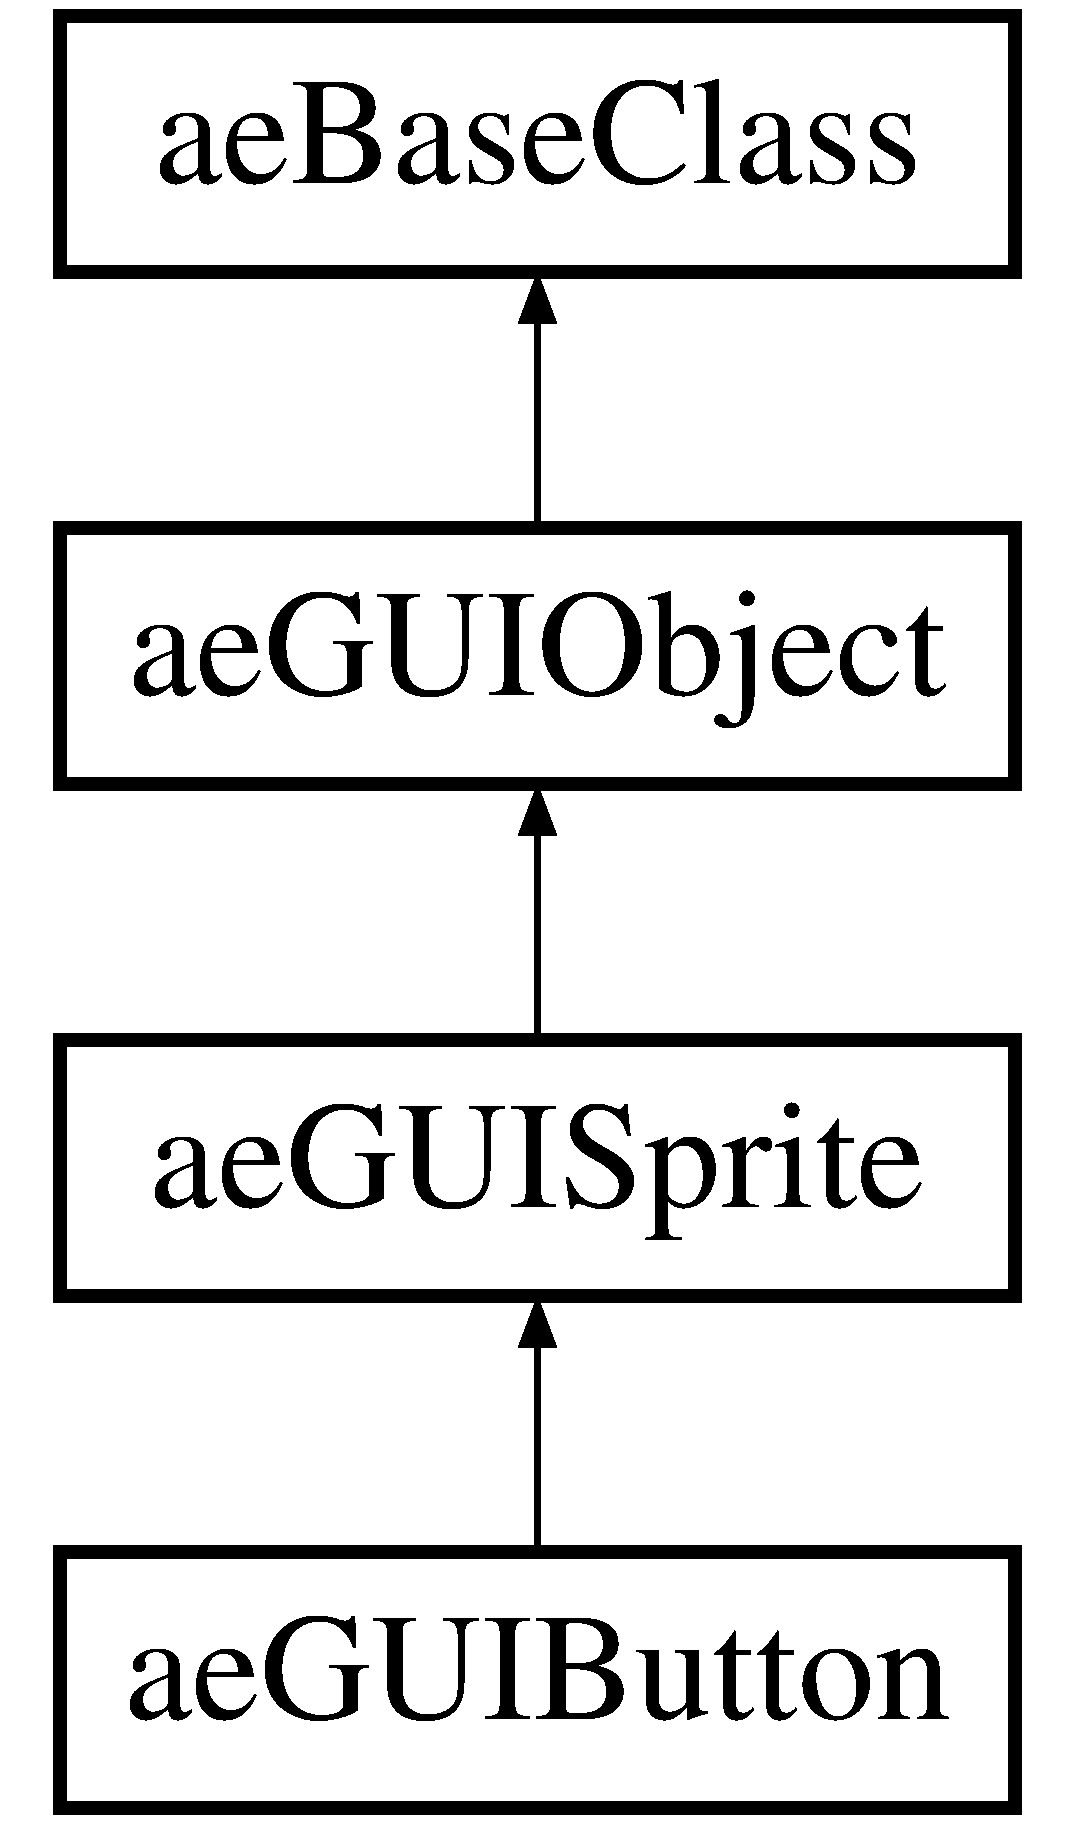
\includegraphics[height=4.000000cm]{classae_g_u_i_button}
\end{center}
\end{figure}
\subsection*{Public Member Functions}
\begin{DoxyCompactItemize}
\item 
Button\+State \hyperlink{classae_g_u_i_button_a873d88936b442e7defdae182ac6b974e}{Get\+State} ()
\begin{DoxyCompactList}\small\item\em Gets the state. \end{DoxyCompactList}\item 
void \hyperlink{classae_g_u_i_button_a4700c24ed5d1a36217dcfdc5dfda41cd}{Click\+On} (\hyperlink{structae_core_1_1ae_point}{ae\+Point} Point)
\begin{DoxyCompactList}\small\item\em Click on. \end{DoxyCompactList}\end{DoxyCompactItemize}
\subsection*{Additional Inherited Members}


\subsection{Detailed Description}
A graphical user interface button. 

\subsection{Member Function Documentation}
\index{ae\+G\+U\+I\+Button@{ae\+G\+U\+I\+Button}!Click\+On@{Click\+On}}
\index{Click\+On@{Click\+On}!ae\+G\+U\+I\+Button@{ae\+G\+U\+I\+Button}}
\subsubsection[{\texorpdfstring{Click\+On(ae\+Point Point)}{ClickOn(aePoint Point)}}]{\setlength{\rightskip}{0pt plus 5cm}void ae\+G\+U\+I\+Button\+::\+Click\+On (
\begin{DoxyParamCaption}
\item[{{\bf ae\+Point}}]{Point}
\end{DoxyParamCaption}
)}\hypertarget{classae_g_u_i_button_a4700c24ed5d1a36217dcfdc5dfda41cd}{}\label{classae_g_u_i_button_a4700c24ed5d1a36217dcfdc5dfda41cd}


Click on. 


\begin{DoxyParams}{Parameters}
{\em Point} & The point. \\
\hline
\end{DoxyParams}
\index{ae\+G\+U\+I\+Button@{ae\+G\+U\+I\+Button}!Get\+State@{Get\+State}}
\index{Get\+State@{Get\+State}!ae\+G\+U\+I\+Button@{ae\+G\+U\+I\+Button}}
\subsubsection[{\texorpdfstring{Get\+State()}{GetState()}}]{\setlength{\rightskip}{0pt plus 5cm}Button\+State ae\+G\+U\+I\+Button\+::\+Get\+State (
\begin{DoxyParamCaption}
{}
\end{DoxyParamCaption}
)}\hypertarget{classae_g_u_i_button_a873d88936b442e7defdae182ac6b974e}{}\label{classae_g_u_i_button_a873d88936b442e7defdae182ac6b974e}


Gets the state. 

\begin{DoxyReturn}{Returns}
The state. 
\end{DoxyReturn}


The documentation for this class was generated from the following files\+:\begin{DoxyCompactItemize}
\item 
C\+:/\+Users/\+Alvaro Estrada/\+Documents/\+Visual Studio 2015/\+Projects/\+R\+T\+S\+\_\+\+A\+E/\+R\+T\+S\+\_\+\+A\+E/\+Game/G\+U\+I\+Button.\+h\item 
C\+:/\+Users/\+Alvaro Estrada/\+Documents/\+Visual Studio 2015/\+Projects/\+R\+T\+S\+\_\+\+A\+E/\+R\+T\+S\+\_\+\+A\+E/\+Game/\hyperlink{_g_u_i_button_8cpp}{G\+U\+I\+Button.\+cpp}\end{DoxyCompactItemize}

\hypertarget{classae_g_u_i_object}{}\section{ae\+G\+U\+I\+Object Class Reference}
\label{classae_g_u_i_object}\index{ae\+G\+U\+I\+Object@{ae\+G\+U\+I\+Object}}


A graphical user interface object.  




{\ttfamily \#include $<$G\+U\+I\+Object.\+h$>$}

Inheritance diagram for ae\+G\+U\+I\+Object\+:\begin{figure}[H]
\begin{center}
\leavevmode
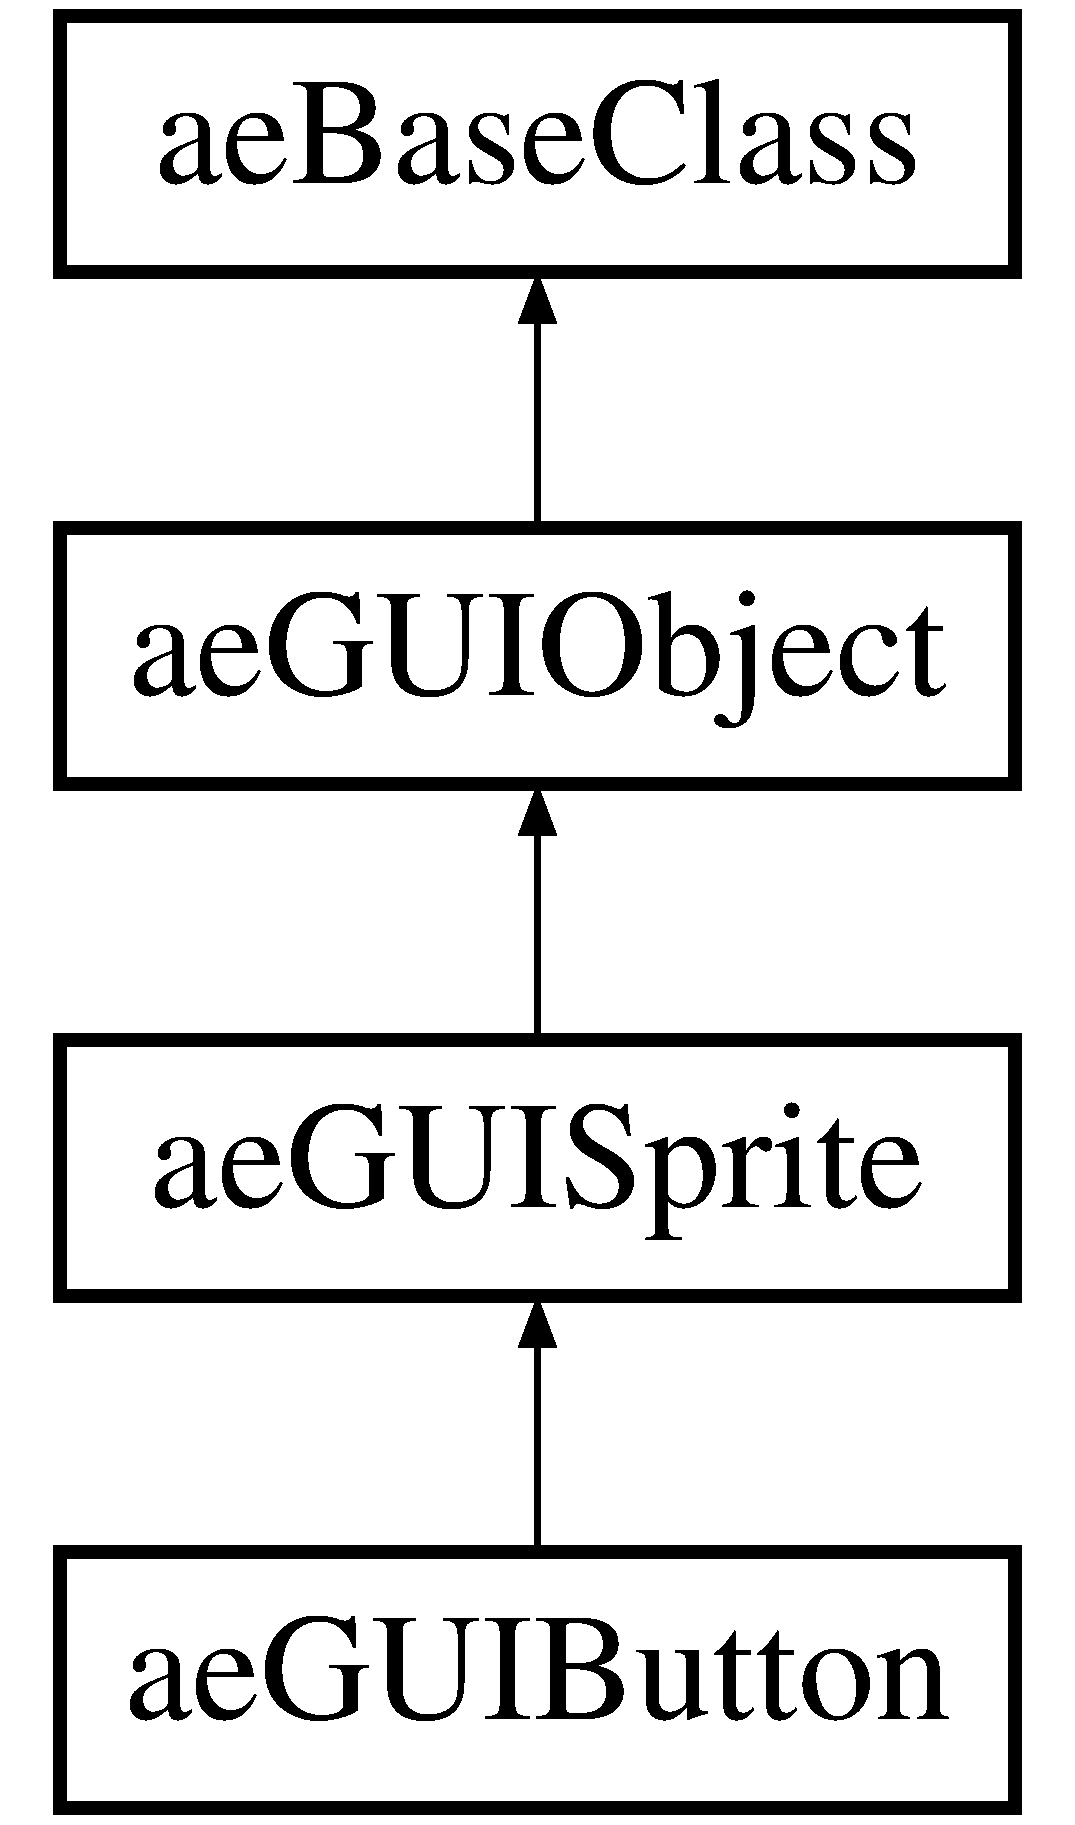
\includegraphics[height=4.000000cm]{classae_g_u_i_object}
\end{center}
\end{figure}
\subsection*{Public Member Functions}
\begin{DoxyCompactItemize}
\item 
virtual int \hyperlink{classae_g_u_i_object_a7a3af664fd1650365a863ea84723c857}{Init} ()
\begin{DoxyCompactList}\small\item\em Gets the init. \end{DoxyCompactList}\item 
virtual void \hyperlink{classae_g_u_i_object_a99f3c290206292214fd7caa214875169}{Update} (float f\+Delta)
\begin{DoxyCompactList}\small\item\em Updates the given f\+Delta. \end{DoxyCompactList}\item 
virtual void \hyperlink{classae_g_u_i_object_a6cda0c5222c9d0a9915712c3b2f29090}{Render} (\hyperlink{classae_core_1_1ae_renderer}{ae\+Renderer} $\ast$p\+Renderer)
\begin{DoxyCompactList}\small\item\em Renders the given p\+Renderer. \end{DoxyCompactList}\item 
virtual void \hyperlink{classae_g_u_i_object_afda42b1e96942ad46379b468fd75359c}{Destroy} ()\hypertarget{classae_g_u_i_object_afda42b1e96942ad46379b468fd75359c}{}\label{classae_g_u_i_object_afda42b1e96942ad46379b468fd75359c}

\begin{DoxyCompactList}\small\item\em Destroys this object. \end{DoxyCompactList}\item 
G\+U\+I\+Objects\+ID \hyperlink{classae_g_u_i_object_a3bcd6d568f058891c59a1e9b700d9427}{Get\+Object\+ID} ()
\begin{DoxyCompactList}\small\item\em Gets object identifier. \end{DoxyCompactList}\end{DoxyCompactItemize}
\subsection*{Public Attributes}
\begin{DoxyCompactItemize}
\item 
ae\+Point {\bfseries Position}\hypertarget{classae_g_u_i_object_ac4d0c937ed1fbe0c27430a26b7140c4b}{}\label{classae_g_u_i_object_ac4d0c937ed1fbe0c27430a26b7140c4b}

\item 
ae\+String {\bfseries Name}\hypertarget{classae_g_u_i_object_acf409a193d1897123657ea8646de33de}{}\label{classae_g_u_i_object_acf409a193d1897123657ea8646de33de}

\item 
ae\+String {\bfseries Tag}\hypertarget{classae_g_u_i_object_ae95d430e3495e894f344dd8ec36231d8}{}\label{classae_g_u_i_object_ae95d430e3495e894f344dd8ec36231d8}

\item 
\hyperlink{_add_on_8h_a0f4072611b509766afe7bb36d570ac80}{ae\+Add\+Ons} {\bfseries Add\+Ons}\hypertarget{classae_g_u_i_object_a10f12fc957daf9baf020a099c29e0f6a}{}\label{classae_g_u_i_object_a10f12fc957daf9baf020a099c29e0f6a}

\end{DoxyCompactItemize}
\subsection*{Protected Attributes}
\begin{DoxyCompactItemize}
\item 
G\+U\+I\+Objects\+ID {\bfseries m\+\_\+n\+G\+U\+I\+Object\+ID}\hypertarget{classae_g_u_i_object_afffd1755f6b5e5f9795ccbac72e918c1}{}\label{classae_g_u_i_object_afffd1755f6b5e5f9795ccbac72e918c1}

\end{DoxyCompactItemize}


\subsection{Detailed Description}
A graphical user interface object. 

\subsection{Member Function Documentation}
\index{ae\+G\+U\+I\+Object@{ae\+G\+U\+I\+Object}!Get\+Object\+ID@{Get\+Object\+ID}}
\index{Get\+Object\+ID@{Get\+Object\+ID}!ae\+G\+U\+I\+Object@{ae\+G\+U\+I\+Object}}
\subsubsection[{\texorpdfstring{Get\+Object\+I\+D()}{GetObjectID()}}]{\setlength{\rightskip}{0pt plus 5cm}G\+U\+I\+Objects\+ID ae\+G\+U\+I\+Object\+::\+Get\+Object\+ID (
\begin{DoxyParamCaption}
{}
\end{DoxyParamCaption}
)}\hypertarget{classae_g_u_i_object_a3bcd6d568f058891c59a1e9b700d9427}{}\label{classae_g_u_i_object_a3bcd6d568f058891c59a1e9b700d9427}


Gets object identifier. 

\begin{DoxyReturn}{Returns}
The object identifier. 
\end{DoxyReturn}
\index{ae\+G\+U\+I\+Object@{ae\+G\+U\+I\+Object}!Init@{Init}}
\index{Init@{Init}!ae\+G\+U\+I\+Object@{ae\+G\+U\+I\+Object}}
\subsubsection[{\texorpdfstring{Init()}{Init()}}]{\setlength{\rightskip}{0pt plus 5cm}int ae\+G\+U\+I\+Object\+::\+Init (
\begin{DoxyParamCaption}
{}
\end{DoxyParamCaption}
)\hspace{0.3cm}{\ttfamily [virtual]}}\hypertarget{classae_g_u_i_object_a7a3af664fd1650365a863ea84723c857}{}\label{classae_g_u_i_object_a7a3af664fd1650365a863ea84723c857}


Gets the init. 

\begin{DoxyReturn}{Returns}
An int. 
\end{DoxyReturn}
\index{ae\+G\+U\+I\+Object@{ae\+G\+U\+I\+Object}!Render@{Render}}
\index{Render@{Render}!ae\+G\+U\+I\+Object@{ae\+G\+U\+I\+Object}}
\subsubsection[{\texorpdfstring{Render(ae\+Renderer $\ast$p\+Renderer)}{Render(aeRenderer *pRenderer)}}]{\setlength{\rightskip}{0pt plus 5cm}void ae\+G\+U\+I\+Object\+::\+Render (
\begin{DoxyParamCaption}
\item[{{\bf ae\+Renderer} $\ast$}]{p\+Renderer}
\end{DoxyParamCaption}
)\hspace{0.3cm}{\ttfamily [virtual]}}\hypertarget{classae_g_u_i_object_a6cda0c5222c9d0a9915712c3b2f29090}{}\label{classae_g_u_i_object_a6cda0c5222c9d0a9915712c3b2f29090}


Renders the given p\+Renderer. 


\begin{DoxyParams}[1]{Parameters}
\mbox{\tt in,out}  & {\em p\+Renderer} & If non-\/null, the renderer. \\
\hline
\end{DoxyParams}
\index{ae\+G\+U\+I\+Object@{ae\+G\+U\+I\+Object}!Update@{Update}}
\index{Update@{Update}!ae\+G\+U\+I\+Object@{ae\+G\+U\+I\+Object}}
\subsubsection[{\texorpdfstring{Update(float f\+Delta)}{Update(float fDelta)}}]{\setlength{\rightskip}{0pt plus 5cm}void ae\+G\+U\+I\+Object\+::\+Update (
\begin{DoxyParamCaption}
\item[{float}]{f\+Delta}
\end{DoxyParamCaption}
)\hspace{0.3cm}{\ttfamily [virtual]}}\hypertarget{classae_g_u_i_object_a99f3c290206292214fd7caa214875169}{}\label{classae_g_u_i_object_a99f3c290206292214fd7caa214875169}


Updates the given f\+Delta. 


\begin{DoxyParams}{Parameters}
{\em f\+Delta} & The delta. \\
\hline
\end{DoxyParams}


The documentation for this class was generated from the following files\+:\begin{DoxyCompactItemize}
\item 
C\+:/\+Users/\+Alvaro Estrada/\+Documents/\+Visual Studio 2015/\+Projects/\+R\+T\+S\+\_\+\+A\+E/\+R\+T\+S\+\_\+\+A\+E/\+Game/G\+U\+I\+Object.\+h\item 
C\+:/\+Users/\+Alvaro Estrada/\+Documents/\+Visual Studio 2015/\+Projects/\+R\+T\+S\+\_\+\+A\+E/\+R\+T\+S\+\_\+\+A\+E/\+Game/G\+U\+I\+Object.\+cpp\end{DoxyCompactItemize}

\hypertarget{classae_g_u_i_sprite}{}\section{ae\+G\+U\+I\+Sprite Class Reference}
\label{classae_g_u_i_sprite}\index{ae\+G\+U\+I\+Sprite@{ae\+G\+U\+I\+Sprite}}


A graphical user interface sprite.  




{\ttfamily \#include $<$G\+U\+I\+Sprite.\+h$>$}

Inheritance diagram for ae\+G\+U\+I\+Sprite\+:\begin{figure}[H]
\begin{center}
\leavevmode
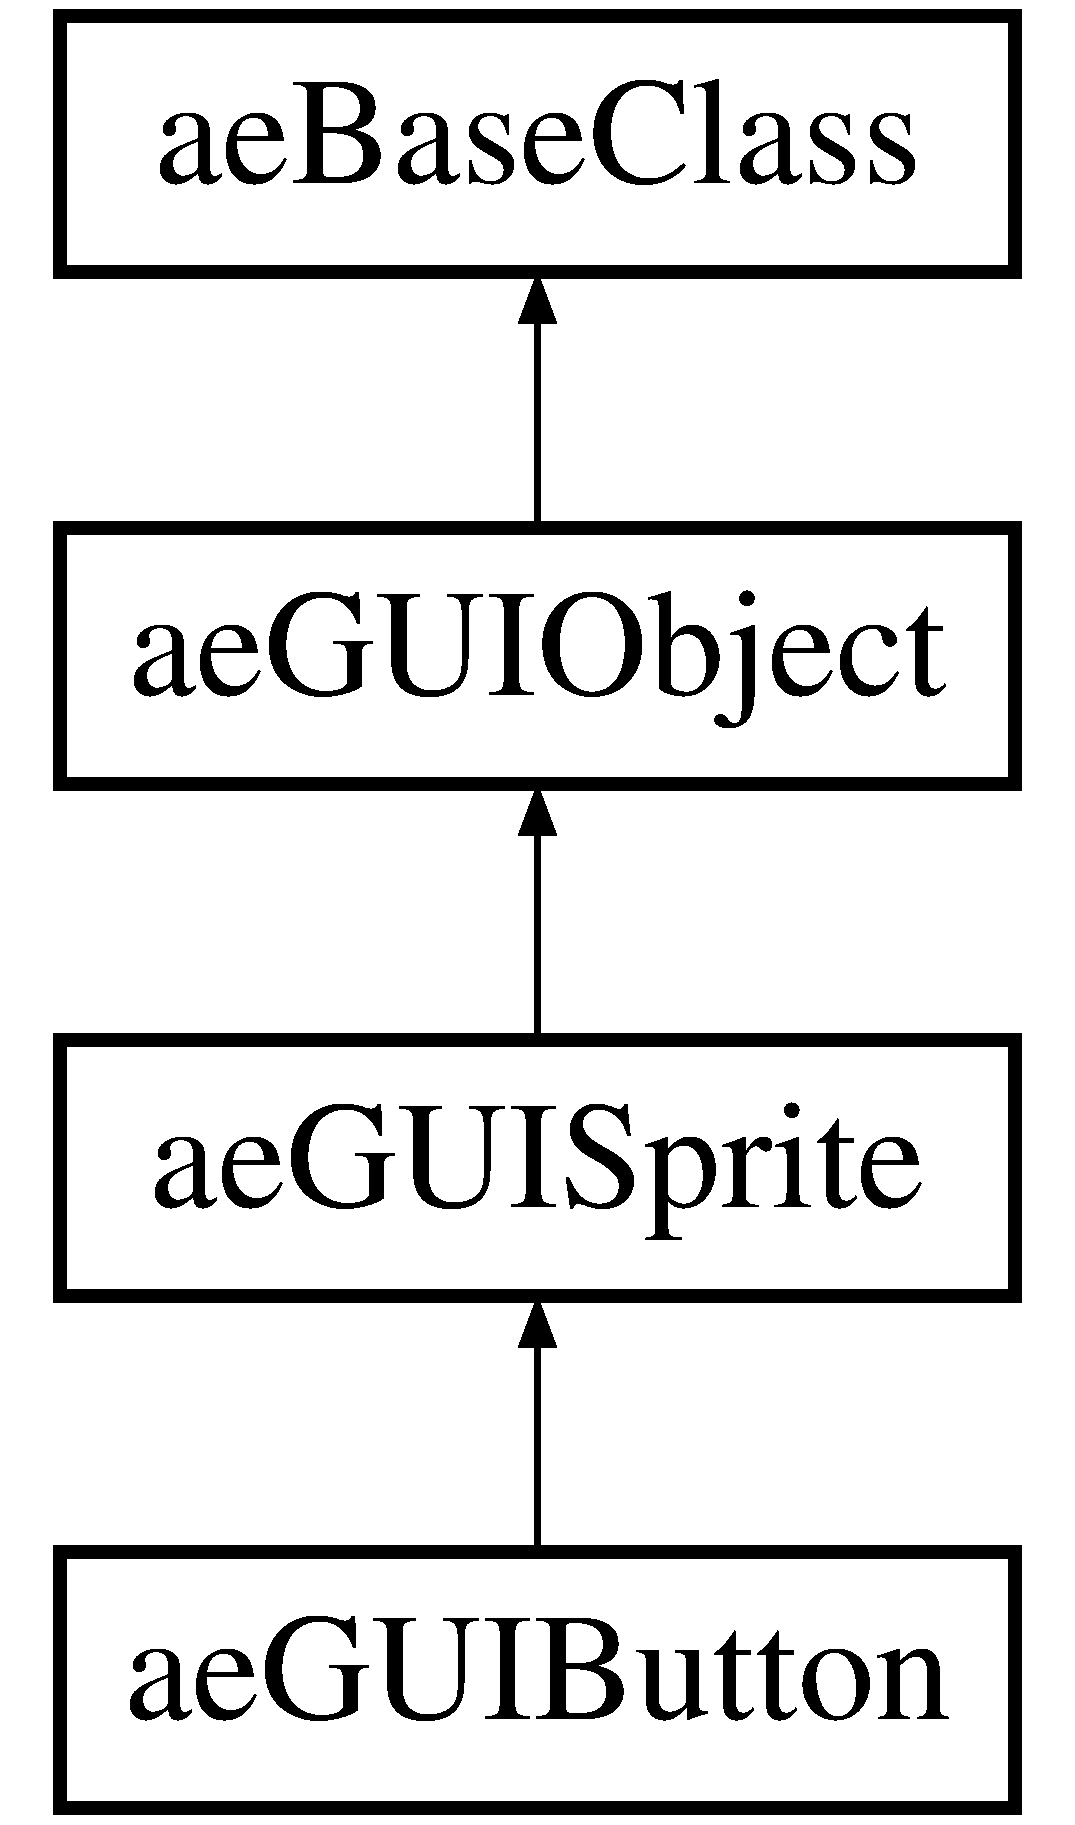
\includegraphics[height=4.000000cm]{classae_g_u_i_sprite}
\end{center}
\end{figure}
\subsection*{Public Member Functions}
\begin{DoxyCompactItemize}
\item 
virtual int {\bfseries Init} (\hyperlink{structae_core_1_1ae_point}{ae\+Point} Displacement, \hyperlink{classae_core_1_1ae_sprite}{ae\+Sprite} $\ast$p\+Sprite)\hypertarget{classae_g_u_i_sprite_a2c6520841e2da9860d2834ef199b314a}{}\label{classae_g_u_i_sprite_a2c6520841e2da9860d2834ef199b314a}

\item 
virtual void \hyperlink{classae_g_u_i_sprite_a4b4d3427fe8adbc4a575b5313743aa7d}{Destroy} ()\hypertarget{classae_g_u_i_sprite_a4b4d3427fe8adbc4a575b5313743aa7d}{}\label{classae_g_u_i_sprite_a4b4d3427fe8adbc4a575b5313743aa7d}

\begin{DoxyCompactList}\small\item\em Destroys this object. \end{DoxyCompactList}\end{DoxyCompactItemize}
\subsection*{Protected Attributes}
\begin{DoxyCompactItemize}
\item 
ae\+Sprite $\ast$ {\bfseries m\+\_\+p\+Sprite}\hypertarget{classae_g_u_i_sprite_a68c442299ee5560144baba573e8a4d7f}{}\label{classae_g_u_i_sprite_a68c442299ee5560144baba573e8a4d7f}

\item 
ae\+Rect {\bfseries m\+\_\+\+Rect}\hypertarget{classae_g_u_i_sprite_a3d3215806d267a9663ed0e947c5041b1}{}\label{classae_g_u_i_sprite_a3d3215806d267a9663ed0e947c5041b1}

\end{DoxyCompactItemize}
\subsection*{Additional Inherited Members}


\subsection{Detailed Description}
A graphical user interface sprite. 

The documentation for this class was generated from the following files\+:\begin{DoxyCompactItemize}
\item 
C\+:/\+Users/\+Alvaro Estrada/\+Documents/\+Visual Studio 2015/\+Projects/\+R\+T\+S\+\_\+\+A\+E/\+R\+T\+S\+\_\+\+A\+E/\+Game/G\+U\+I\+Sprite.\+h\item 
C\+:/\+Users/\+Alvaro Estrada/\+Documents/\+Visual Studio 2015/\+Projects/\+R\+T\+S\+\_\+\+A\+E/\+R\+T\+S\+\_\+\+A\+E/\+Game/G\+U\+I\+Sprite.\+cpp\end{DoxyCompactItemize}

\hypertarget{classae_influence_calculator}{}\section{ae\+Influence\+Calculator Class Reference}
\label{classae_influence_calculator}\index{ae\+Influence\+Calculator@{ae\+Influence\+Calculator}}
Inheritance diagram for ae\+Influence\+Calculator\+:\begin{figure}[H]
\begin{center}
\leavevmode
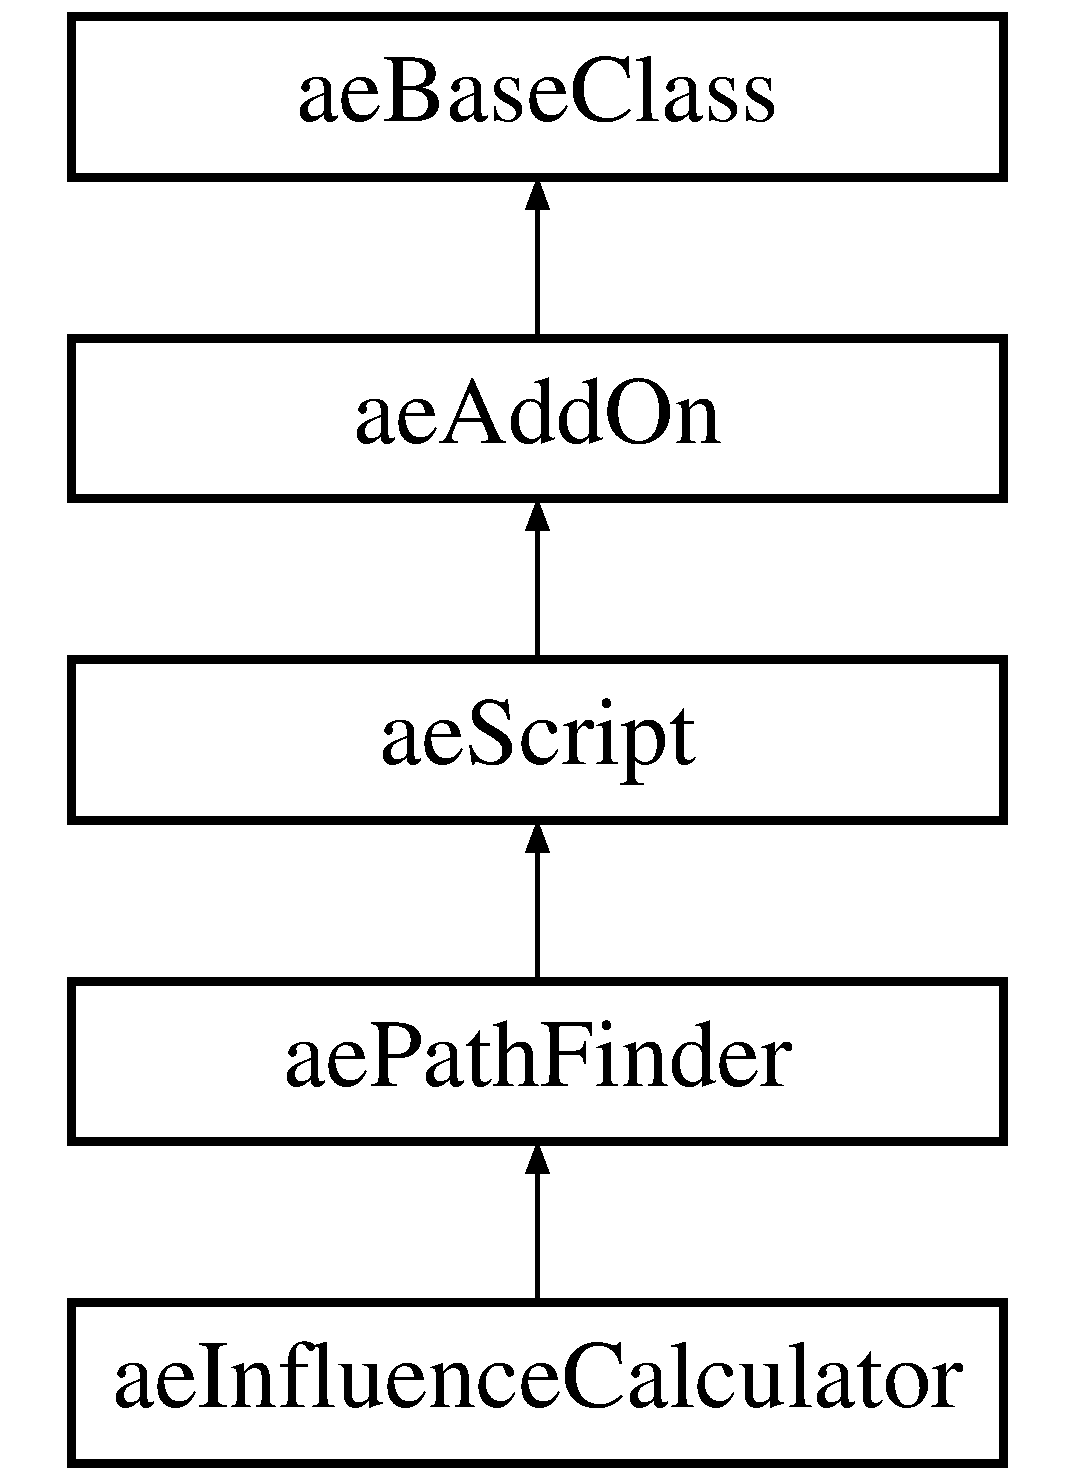
\includegraphics[height=5.000000cm]{classae_influence_calculator}
\end{center}
\end{figure}
\subsection*{Public Member Functions}
\begin{DoxyCompactItemize}
\item 
{\bfseries ae\+Influence\+Calculator} (\hyperlink{classae_tiled_map}{ae\+Tiled\+Map} $\ast$p\+Map)\hypertarget{classae_influence_calculator_aef49d51bfbef33de2603e69a2dac091c}{}\label{classae_influence_calculator_aef49d51bfbef33de2603e69a2dac091c}

\item 
virtual int \hyperlink{classae_influence_calculator_ab2607b3e3750770bb23d7e8c4610a49c}{Init} (\hyperlink{classae_base_class}{ae\+Base\+Class} $\ast$p\+Parent)
\begin{DoxyCompactList}\small\item\em Initializes with the given parent pointer. \end{DoxyCompactList}\item 
virtual void \hyperlink{classae_influence_calculator_a83e784eea5912b82a7ebfe80373f6c2e}{Destroy} ()\hypertarget{classae_influence_calculator_a83e784eea5912b82a7ebfe80373f6c2e}{}\label{classae_influence_calculator_a83e784eea5912b82a7ebfe80373f6c2e}

\begin{DoxyCompactList}\small\item\em Destroys this object. \end{DoxyCompactList}\item 
virtual void \hyperlink{classae_influence_calculator_af1e3be3558a8e0e0638959ca41734abd}{Update} (float f\+Delta)
\begin{DoxyCompactList}\small\item\em Updates the given f\+Delta. \end{DoxyCompactList}\item 
virtual void \hyperlink{classae_influence_calculator_a9c48a833f9f81303ec212a9a17d83920}{Render} (\hyperlink{classae_core_1_1ae_renderer}{ae\+Renderer} $\ast$p\+Renderer)
\begin{DoxyCompactList}\small\item\em Renders the given Renderer pointer. \end{DoxyCompactList}\item 
virtual void \hyperlink{classae_influence_calculator_a78c17fcba2c67a0e62edd2b8a123a825}{Reset} ()\hypertarget{classae_influence_calculator_a78c17fcba2c67a0e62edd2b8a123a825}{}\label{classae_influence_calculator_a78c17fcba2c67a0e62edd2b8a123a825}

\begin{DoxyCompactList}\small\item\em Resets this object. \end{DoxyCompactList}\item 
virtual void \hyperlink{classae_influence_calculator_aa581fbf63f74dc501a366ac264c2f12d}{Set\+Influence\+Points} (\hyperlink{structae_influence_point}{ae\+Influence\+Point} $\ast$Points, int size)
\begin{DoxyCompactList}\small\item\em Sets influence points. \end{DoxyCompactList}\end{DoxyCompactItemize}
\subsection*{Public Attributes}
\begin{DoxyCompactItemize}
\item 
float {\bfseries m\+\_\+f\+Momentum}\hypertarget{classae_influence_calculator_a11f861aacb6c3a58c23b1fa8eabbbc4b}{}\label{classae_influence_calculator_a11f861aacb6c3a58c23b1fa8eabbbc4b}

\item 
float {\bfseries m\+\_\+f\+Decay}\hypertarget{classae_influence_calculator_adde84abe917bba5fcfe453fda73571a6}{}\label{classae_influence_calculator_adde84abe917bba5fcfe453fda73571a6}

\item 
float {\bfseries m\+\_\+f\+Max\+Inf}\hypertarget{classae_influence_calculator_a617f4f4dded2b0078a200907b8101bde}{}\label{classae_influence_calculator_a617f4f4dded2b0078a200907b8101bde}

\item 
float {\bfseries m\+\_\+f\+Min\+Inf}\hypertarget{classae_influence_calculator_a9d3ddc8723c25d95407c74647e3e8287}{}\label{classae_influence_calculator_a9d3ddc8723c25d95407c74647e3e8287}

\item 
float {\bfseries m\+\_\+\+Inf}\hypertarget{classae_influence_calculator_ad41edf8a9a2708f63bd38c211b67736c}{}\label{classae_influence_calculator_ad41edf8a9a2708f63bd38c211b67736c}

\end{DoxyCompactItemize}
\subsection*{Protected Member Functions}
\begin{DoxyCompactItemize}
\item 
virtual void \hyperlink{classae_influence_calculator_a8f31c5a25ca68ef970247f608bb51917}{Visit\+Grid\+Node} (\hyperlink{namespaceae_core_a862bc39eb87cfabca273f49e2a920129}{int32} x, \hyperlink{namespaceae_core_a862bc39eb87cfabca273f49e2a920129}{int32} y)
\begin{DoxyCompactList}\small\item\em Marks a node as visited. \end{DoxyCompactList}\item 
virtual void \hyperlink{classae_influence_calculator_ab542ea1dd26801211d06e77ba078ebe2}{Set\+Final\+Node} (\hyperlink{namespaceae_core_a862bc39eb87cfabca273f49e2a920129}{int32} x, \hyperlink{namespaceae_core_a862bc39eb87cfabca273f49e2a920129}{int32} y)
\begin{DoxyCompactList}\small\item\em Sets final node. \end{DoxyCompactList}\item 
virtual Walk\+State\+ID {\bfseries Give\+A\+Step} (int32 x, int32 y)\hypertarget{classae_influence_calculator_a3195d218f0580918600336418df7daed}{}\label{classae_influence_calculator_a3195d218f0580918600336418df7daed}

\item 
virtual Walk\+State\+ID \hyperlink{classae_influence_calculator_aff6d5b8b52fb73a4c87a3b311adc6245}{Give\+A\+Step} ()
\begin{DoxyCompactList}\small\item\em Give a step. \end{DoxyCompactList}\item 
float {\bfseries lerp} (float Start, float End, float Porcentage)\hypertarget{classae_influence_calculator_a2319a79402f14228159d40380ff9e3b2}{}\label{classae_influence_calculator_a2319a79402f14228159d40380ff9e3b2}

\item 
float {\bfseries Dist} (int x, int y)\hypertarget{classae_influence_calculator_aef42a7d51c210b1ace9861975a5785ac}{}\label{classae_influence_calculator_aef42a7d51c210b1ace9861975a5785ac}

\end{DoxyCompactItemize}
\subsection*{Additional Inherited Members}


\subsection{Member Function Documentation}
\index{ae\+Influence\+Calculator@{ae\+Influence\+Calculator}!Give\+A\+Step@{Give\+A\+Step}}
\index{Give\+A\+Step@{Give\+A\+Step}!ae\+Influence\+Calculator@{ae\+Influence\+Calculator}}
\subsubsection[{\texorpdfstring{Give\+A\+Step()}{GiveAStep()}}]{\setlength{\rightskip}{0pt plus 5cm}Walk\+State\+ID ae\+Influence\+Calculator\+::\+Give\+A\+Step (
\begin{DoxyParamCaption}
{}
\end{DoxyParamCaption}
)\hspace{0.3cm}{\ttfamily [protected]}, {\ttfamily [virtual]}}\hypertarget{classae_influence_calculator_aff6d5b8b52fb73a4c87a3b311adc6245}{}\label{classae_influence_calculator_aff6d5b8b52fb73a4c87a3b311adc6245}


Give a step. 

\begin{DoxyReturn}{Returns}
A Walk\+State\+ID. 
\end{DoxyReturn}


Implements \hyperlink{classae_path_finder_a49332ee3be744cac1ece9ffd503ca218}{ae\+Path\+Finder}.

\index{ae\+Influence\+Calculator@{ae\+Influence\+Calculator}!Init@{Init}}
\index{Init@{Init}!ae\+Influence\+Calculator@{ae\+Influence\+Calculator}}
\subsubsection[{\texorpdfstring{Init(ae\+Base\+Class $\ast$p\+Parent)}{Init(aeBaseClass *pParent)}}]{\setlength{\rightskip}{0pt plus 5cm}int ae\+Influence\+Calculator\+::\+Init (
\begin{DoxyParamCaption}
\item[{{\bf ae\+Base\+Class} $\ast$}]{p\+Parent}
\end{DoxyParamCaption}
)\hspace{0.3cm}{\ttfamily [virtual]}}\hypertarget{classae_influence_calculator_ab2607b3e3750770bb23d7e8c4610a49c}{}\label{classae_influence_calculator_ab2607b3e3750770bb23d7e8c4610a49c}


Initializes with the given parent pointer. 


\begin{DoxyParams}[1]{Parameters}
\mbox{\tt in,out}  & {\em p\+Parent} & If non-\/null, the parent.\\
\hline
\end{DoxyParams}
\begin{DoxyReturn}{Returns}
An int. 
\end{DoxyReturn}


Reimplemented from \hyperlink{classae_path_finder_a3395375f3de8f3f55d7b780ff6815806}{ae\+Path\+Finder}.

\index{ae\+Influence\+Calculator@{ae\+Influence\+Calculator}!Render@{Render}}
\index{Render@{Render}!ae\+Influence\+Calculator@{ae\+Influence\+Calculator}}
\subsubsection[{\texorpdfstring{Render(ae\+Renderer $\ast$p\+Renderer)}{Render(aeRenderer *pRenderer)}}]{\setlength{\rightskip}{0pt plus 5cm}void ae\+Influence\+Calculator\+::\+Render (
\begin{DoxyParamCaption}
\item[{{\bf ae\+Renderer} $\ast$}]{p\+Renderer}
\end{DoxyParamCaption}
)\hspace{0.3cm}{\ttfamily [virtual]}}\hypertarget{classae_influence_calculator_a9c48a833f9f81303ec212a9a17d83920}{}\label{classae_influence_calculator_a9c48a833f9f81303ec212a9a17d83920}


Renders the given Renderer pointer. 


\begin{DoxyParams}[1]{Parameters}
\mbox{\tt in,out}  & {\em p\+Renderer} & If non-\/null, the renderer. \\
\hline
\end{DoxyParams}


Reimplemented from \hyperlink{classae_add_on_ab6bed56009b9c92df8ae017a27587dc3}{ae\+Add\+On}.

\index{ae\+Influence\+Calculator@{ae\+Influence\+Calculator}!Set\+Final\+Node@{Set\+Final\+Node}}
\index{Set\+Final\+Node@{Set\+Final\+Node}!ae\+Influence\+Calculator@{ae\+Influence\+Calculator}}
\subsubsection[{\texorpdfstring{Set\+Final\+Node(int32 x, int32 y)}{SetFinalNode(int32 x, int32 y)}}]{\setlength{\rightskip}{0pt plus 5cm}void ae\+Influence\+Calculator\+::\+Set\+Final\+Node (
\begin{DoxyParamCaption}
\item[{{\bf int32}}]{x, }
\item[{{\bf int32}}]{y}
\end{DoxyParamCaption}
)\hspace{0.3cm}{\ttfamily [protected]}, {\ttfamily [virtual]}}\hypertarget{classae_influence_calculator_ab542ea1dd26801211d06e77ba078ebe2}{}\label{classae_influence_calculator_ab542ea1dd26801211d06e77ba078ebe2}


Sets final node. 


\begin{DoxyParams}{Parameters}
{\em x} & The x coordinate. \\
\hline
{\em y} & The y coordinate. \\
\hline
\end{DoxyParams}
\index{ae\+Influence\+Calculator@{ae\+Influence\+Calculator}!Set\+Influence\+Points@{Set\+Influence\+Points}}
\index{Set\+Influence\+Points@{Set\+Influence\+Points}!ae\+Influence\+Calculator@{ae\+Influence\+Calculator}}
\subsubsection[{\texorpdfstring{Set\+Influence\+Points(ae\+Influence\+Point $\ast$\+Points, int size)}{SetInfluencePoints(aeInfluencePoint *Points, int size)}}]{\setlength{\rightskip}{0pt plus 5cm}void ae\+Influence\+Calculator\+::\+Set\+Influence\+Points (
\begin{DoxyParamCaption}
\item[{{\bf ae\+Influence\+Point} $\ast$}]{Points, }
\item[{int}]{size}
\end{DoxyParamCaption}
)\hspace{0.3cm}{\ttfamily [virtual]}}\hypertarget{classae_influence_calculator_aa581fbf63f74dc501a366ac264c2f12d}{}\label{classae_influence_calculator_aa581fbf63f74dc501a366ac264c2f12d}


Sets influence points. 


\begin{DoxyParams}[1]{Parameters}
\mbox{\tt in,out}  & {\em Points} & If non-\/null, the points. \\
\hline
 & {\em size} & The size. \\
\hline
\end{DoxyParams}
\index{ae\+Influence\+Calculator@{ae\+Influence\+Calculator}!Update@{Update}}
\index{Update@{Update}!ae\+Influence\+Calculator@{ae\+Influence\+Calculator}}
\subsubsection[{\texorpdfstring{Update(float f\+Delta)}{Update(float fDelta)}}]{\setlength{\rightskip}{0pt plus 5cm}void ae\+Influence\+Calculator\+::\+Update (
\begin{DoxyParamCaption}
\item[{float}]{f\+Delta}
\end{DoxyParamCaption}
)\hspace{0.3cm}{\ttfamily [virtual]}}\hypertarget{classae_influence_calculator_af1e3be3558a8e0e0638959ca41734abd}{}\label{classae_influence_calculator_af1e3be3558a8e0e0638959ca41734abd}


Updates the given f\+Delta. 


\begin{DoxyParams}{Parameters}
{\em f\+Delta} & The delta. \\
\hline
\end{DoxyParams}


Implements \hyperlink{classae_add_on_a51caa4b8680206495ea671e71991e231}{ae\+Add\+On}.

\index{ae\+Influence\+Calculator@{ae\+Influence\+Calculator}!Visit\+Grid\+Node@{Visit\+Grid\+Node}}
\index{Visit\+Grid\+Node@{Visit\+Grid\+Node}!ae\+Influence\+Calculator@{ae\+Influence\+Calculator}}
\subsubsection[{\texorpdfstring{Visit\+Grid\+Node(int32 x, int32 y)}{VisitGridNode(int32 x, int32 y)}}]{\setlength{\rightskip}{0pt plus 5cm}void ae\+Influence\+Calculator\+::\+Visit\+Grid\+Node (
\begin{DoxyParamCaption}
\item[{{\bf int32}}]{x, }
\item[{{\bf int32}}]{y}
\end{DoxyParamCaption}
)\hspace{0.3cm}{\ttfamily [protected]}, {\ttfamily [virtual]}}\hypertarget{classae_influence_calculator_a8f31c5a25ca68ef970247f608bb51917}{}\label{classae_influence_calculator_a8f31c5a25ca68ef970247f608bb51917}


Marks a node as visited. 


\begin{DoxyParams}{Parameters}
{\em x} & The x coordinate. \\
\hline
{\em y} & The y coordinate. \\
\hline
\end{DoxyParams}


Implements \hyperlink{classae_path_finder_a4ccfa19ff344b9f4827dbeab18c4efab}{ae\+Path\+Finder}.



The documentation for this class was generated from the following files\+:\begin{DoxyCompactItemize}
\item 
C\+:/\+Users/\+Alvaro Estrada/\+Documents/\+Visual Studio 2015/\+Projects/\+R\+T\+S\+\_\+\+A\+E/\+R\+T\+S\+\_\+\+A\+E/\+Game/Influence\+Calculator.\+h\item 
C\+:/\+Users/\+Alvaro Estrada/\+Documents/\+Visual Studio 2015/\+Projects/\+R\+T\+S\+\_\+\+A\+E/\+R\+T\+S\+\_\+\+A\+E/\+Game/Influence\+Calculator.\+cpp\end{DoxyCompactItemize}

\hypertarget{structae_influence_point}{}\section{ae\+Influence\+Point Struct Reference}
\label{structae_influence_point}\index{ae\+Influence\+Point@{ae\+Influence\+Point}}
\subsection*{Public Attributes}
\begin{DoxyCompactItemize}
\item 
float {\bfseries Influence}\hypertarget{structae_influence_point_a383de093611ac1428e692d271a1a040b}{}\label{structae_influence_point_a383de093611ac1428e692d271a1a040b}

\item 
int32 {\bfseries x}\hypertarget{structae_influence_point_a81c35fec8cc72f771b194928f56444e3}{}\label{structae_influence_point_a81c35fec8cc72f771b194928f56444e3}

\item 
int32 {\bfseries y}\hypertarget{structae_influence_point_a57ac80f0f5ed9e1fec3486225e355afb}{}\label{structae_influence_point_a57ac80f0f5ed9e1fec3486225e355afb}

\end{DoxyCompactItemize}


The documentation for this struct was generated from the following file\+:\begin{DoxyCompactItemize}
\item 
C\+:/\+Users/\+Alvaro Estrada/\+Documents/\+Visual Studio 2015/\+Projects/\+R\+T\+S\+\_\+\+A\+E/\+R\+T\+S\+\_\+\+A\+E/\+Game/Influence\+Calculator.\+h\end{DoxyCompactItemize}

\hypertarget{classae_influence_tile_node}{}\section{ae\+Influence\+Tile\+Node Class Reference}
\label{classae_influence_tile_node}\index{ae\+Influence\+Tile\+Node@{ae\+Influence\+Tile\+Node}}
Inheritance diagram for ae\+Influence\+Tile\+Node\+:\begin{figure}[H]
\begin{center}
\leavevmode
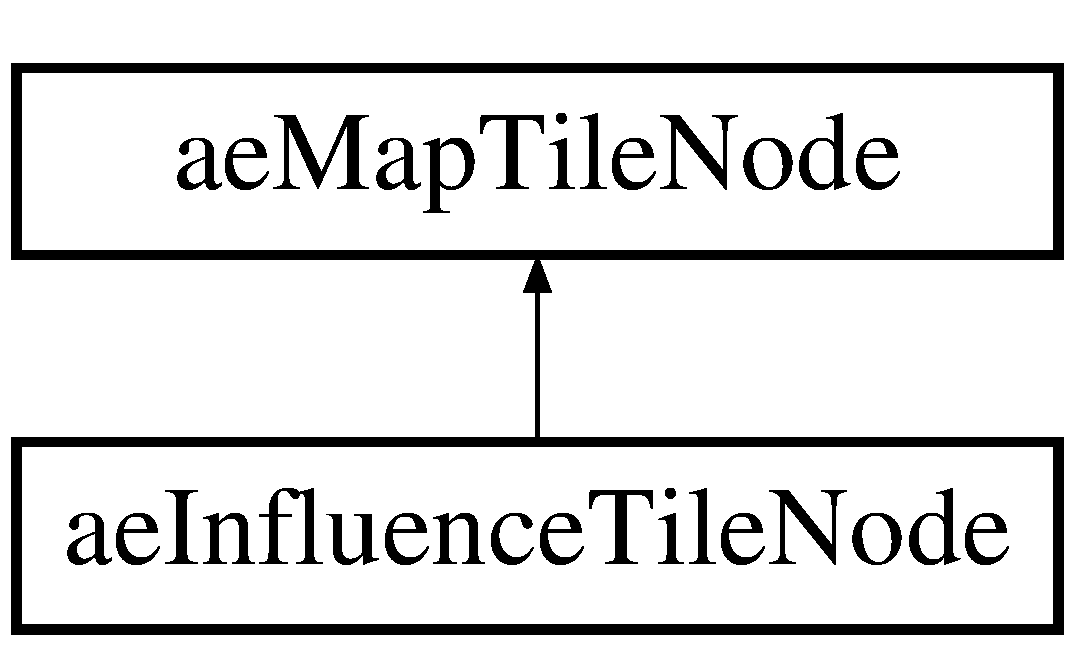
\includegraphics[height=2.000000cm]{classae_influence_tile_node}
\end{center}
\end{figure}
\subsection*{Public Member Functions}
\begin{DoxyCompactItemize}
\item 
{\bfseries ae\+Influence\+Tile\+Node} (const \hyperlink{classae_influence_tile_node}{ae\+Influence\+Tile\+Node} \&copy)\hypertarget{classae_influence_tile_node_a415b33425cedb8c0558d61d120b96fc9}{}\label{classae_influence_tile_node_a415b33425cedb8c0558d61d120b96fc9}

\item 
virtual \hyperlink{classae_influence_tile_node}{ae\+Influence\+Tile\+Node} \& {\bfseries operator=} (const \hyperlink{classae_influence_tile_node}{ae\+Influence\+Tile\+Node} \&rhs)\hypertarget{classae_influence_tile_node_aef399505bbf95bcc118b4c83c9181d3a}{}\label{classae_influence_tile_node_aef399505bbf95bcc118b4c83c9181d3a}

\item 
virtual void {\bfseries Set\+Influence} (const float cost)\hypertarget{classae_influence_tile_node_af25e541924861a55467bdd81a53fd347}{}\label{classae_influence_tile_node_af25e541924861a55467bdd81a53fd347}

\item 
virtual float {\bfseries Get\+Influence} () const \hypertarget{classae_influence_tile_node_a3b86d1584e70e8fb4228aed0b24309bf}{}\label{classae_influence_tile_node_a3b86d1584e70e8fb4228aed0b24309bf}

\end{DoxyCompactItemize}
\subsection*{Public Attributes}
\begin{DoxyCompactItemize}
\item 
float {\bfseries m\+\_\+f\+Influence}\hypertarget{classae_influence_tile_node_a0a4bbf4098305c2b632b3634e86ccc3a}{}\label{classae_influence_tile_node_a0a4bbf4098305c2b632b3634e86ccc3a}

\end{DoxyCompactItemize}


The documentation for this class was generated from the following files\+:\begin{DoxyCompactItemize}
\item 
C\+:/\+Users/\+Alvaro Estrada/\+Documents/\+Visual Studio 2015/\+Projects/\+R\+T\+S\+\_\+\+A\+E/\+R\+T\+S\+\_\+\+A\+E/\+Game/\hyperlink{_map_tile_node_8h}{Map\+Tile\+Node.\+h}\item 
C\+:/\+Users/\+Alvaro Estrada/\+Documents/\+Visual Studio 2015/\+Projects/\+R\+T\+S\+\_\+\+A\+E/\+R\+T\+S\+\_\+\+A\+E/\+Game/\hyperlink{_map_tile_node_8cpp}{Map\+Tile\+Node.\+cpp}\end{DoxyCompactItemize}

\hypertarget{structae_core_1_1ae_inputs}{}\section{ae\+Core\+:\+:ae\+Inputs Class Reference}
\label{structae_core_1_1ae_inputs}\index{ae\+Core\+::ae\+Inputs@{ae\+Core\+::ae\+Inputs}}


It\textquotesingle{}s a class compounded of all the type of inputs admitted.  




{\ttfamily \#include $<$Inputs.\+h$>$}

\subsection*{Public Member Functions}
\begin{DoxyCompactItemize}
\item 
int {\bfseries Init} ()\hypertarget{structae_core_1_1ae_inputs_a6e5a34a96a504703797f4e6046d5fe78}{}\label{structae_core_1_1ae_inputs_a6e5a34a96a504703797f4e6046d5fe78}

\item 
void {\bfseries Update} ()\hypertarget{structae_core_1_1ae_inputs_aab43c15f6e2503872f4b898b486c8e72}{}\label{structae_core_1_1ae_inputs_aab43c15f6e2503872f4b898b486c8e72}

\end{DoxyCompactItemize}
\subsection*{Public Attributes}
\begin{DoxyCompactItemize}
\item 
\hyperlink{classae_core_1_1ae_keyboard}{ae\+Keyboard} {\bfseries Keyboard}\hypertarget{structae_core_1_1ae_inputs_a5b0ac77afe82cec2a50ea4bb24426d27}{}\label{structae_core_1_1ae_inputs_a5b0ac77afe82cec2a50ea4bb24426d27}

\item 
\hyperlink{classae_core_1_1ae_mouse}{ae\+Mouse} {\bfseries Mouse}\hypertarget{structae_core_1_1ae_inputs_a7320366cc9b04bae5f956fa749ab9e43}{}\label{structae_core_1_1ae_inputs_a7320366cc9b04bae5f956fa749ab9e43}

\end{DoxyCompactItemize}


\subsection{Detailed Description}
It\textquotesingle{}s a class compounded of all the type of inputs admitted. 

The documentation for this class was generated from the following files\+:\begin{DoxyCompactItemize}
\item 
C\+:/\+Users/\+Alvaro Estrada/\+Documents/\+Visual Studio 2015/\+Projects/\+R\+T\+S\+\_\+\+A\+E/ae\+Core/\+Event\+System/Inputs.\+h\item 
C\+:/\+Users/\+Alvaro Estrada/\+Documents/\+Visual Studio 2015/\+Projects/\+R\+T\+S\+\_\+\+A\+E/ae\+Core/\+Event\+System/Inputs.\+cpp\end{DoxyCompactItemize}

\hypertarget{classae_core_1_1ae_keyboard}{}\section{ae\+Core\+:\+:ae\+Keyboard Class Reference}
\label{classae_core_1_1ae_keyboard}\index{ae\+Core\+::ae\+Keyboard@{ae\+Core\+::ae\+Keyboard}}


A keyboard.  




{\ttfamily \#include $<$Inputs.\+h$>$}

\subsection*{Public Member Functions}
\begin{DoxyCompactItemize}
\item 
int {\bfseries Init} ()\hypertarget{classae_core_1_1ae_keyboard_ad3514f4fa8fdf101456e10194b8c7409}{}\label{classae_core_1_1ae_keyboard_ad3514f4fa8fdf101456e10194b8c7409}

\item 
void {\bfseries Update} ()\hypertarget{classae_core_1_1ae_keyboard_a50918fe2fd413008f7d6740a4b461736}{}\label{classae_core_1_1ae_keyboard_a50918fe2fd413008f7d6740a4b461736}

\item 
\hyperlink{namespaceae_core_aa7afae6827a908a9adc5250cf17d52cb}{Key\+States\+Decode} {\bfseries operator\mbox{[}$\,$\mbox{]}} (int Key)\hypertarget{classae_core_1_1ae_keyboard_a4a7046fe89f379e59c14ffc1a4593a99}{}\label{classae_core_1_1ae_keyboard_a4a7046fe89f379e59c14ffc1a4593a99}

\end{DoxyCompactItemize}
\subsection*{Protected Attributes}
\begin{DoxyCompactItemize}
\item 
std\+::array$<$ \hyperlink{namespaceae_core_aa13093dc911869e5b24942552898f01f}{uint8}, 256 $>$ {\bfseries m\+\_\+p\+Last\+State}\hypertarget{classae_core_1_1ae_keyboard_aa9edb16b75d5a1a90e047d92266a4ee3}{}\label{classae_core_1_1ae_keyboard_aa9edb16b75d5a1a90e047d92266a4ee3}

\item 
std\+::array$<$ \hyperlink{namespaceae_core_aa13093dc911869e5b24942552898f01f}{uint8}, 256 $>$ {\bfseries m\+\_\+p\+Current\+State}\hypertarget{classae_core_1_1ae_keyboard_ac5b064e8ad23f19dcba4555cd2905ba5}{}\label{classae_core_1_1ae_keyboard_ac5b064e8ad23f19dcba4555cd2905ba5}

\end{DoxyCompactItemize}


\subsection{Detailed Description}
A keyboard. 

The documentation for this class was generated from the following files\+:\begin{DoxyCompactItemize}
\item 
C\+:/\+Users/\+Alvaro Estrada/\+Documents/\+Visual Studio 2015/\+Projects/\+R\+T\+S\+\_\+\+A\+E/ae\+Core/\+Event\+System/Inputs.\+h\item 
C\+:/\+Users/\+Alvaro Estrada/\+Documents/\+Visual Studio 2015/\+Projects/\+R\+T\+S\+\_\+\+A\+E/ae\+Core/\+Event\+System/Inputs.\+cpp\end{DoxyCompactItemize}

\hypertarget{structae_core_1_1ae_keyboard_event}{}\section{ae\+Core\+:\+:ae\+Keyboard\+Event Struct Reference}
\label{structae_core_1_1ae_keyboard_event}\index{ae\+Core\+::ae\+Keyboard\+Event@{ae\+Core\+::ae\+Keyboard\+Event}}


A Keyboard message.  




{\ttfamily \#include $<$Events\+System.\+h$>$}

Inheritance diagram for ae\+Core\+:\+:ae\+Keyboard\+Event\+:\begin{figure}[H]
\begin{center}
\leavevmode
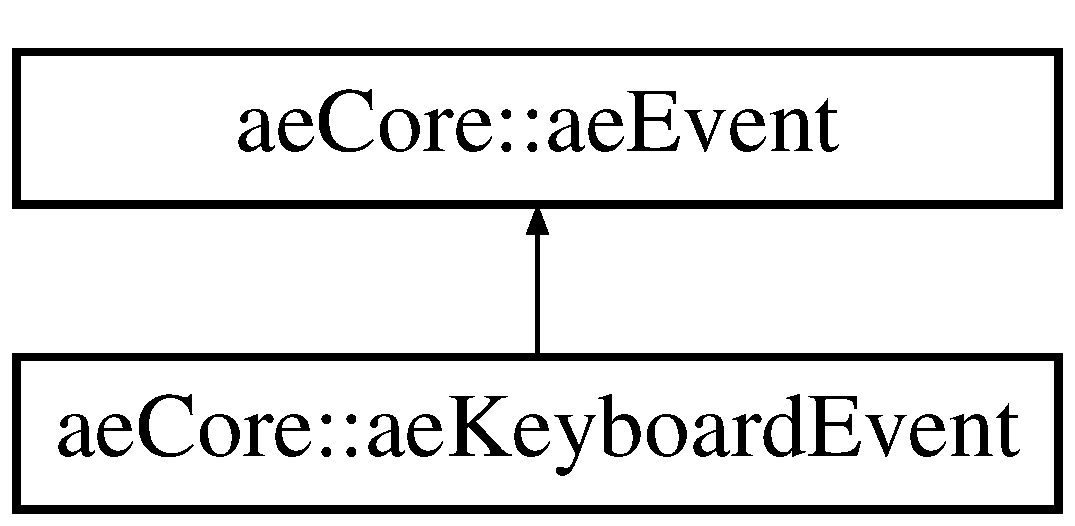
\includegraphics[height=2.000000cm]{structae_core_1_1ae_keyboard_event}
\end{center}
\end{figure}
\subsection*{Public Attributes}
\begin{DoxyCompactItemize}
\item 
\hyperlink{namespaceae_core_aa13093dc911869e5b24942552898f01f}{uint8} {\bfseries Key}\hypertarget{structae_core_1_1ae_keyboard_event_abceaa0d341cd16e2f5d4e6e32dd3337a}{}\label{structae_core_1_1ae_keyboard_event_abceaa0d341cd16e2f5d4e6e32dd3337a}

\item 
\hyperlink{namespaceae_core_aa13093dc911869e5b24942552898f01f}{uint8} {\bfseries State}\hypertarget{structae_core_1_1ae_keyboard_event_a90a90d911854e7430baf5c454670dc9a}{}\label{structae_core_1_1ae_keyboard_event_a90a90d911854e7430baf5c454670dc9a}

\end{DoxyCompactItemize}


\subsection{Detailed Description}
A Keyboard message. 

The documentation for this struct was generated from the following file\+:\begin{DoxyCompactItemize}
\item 
C\+:/\+Users/\+Alvaro Estrada/\+Documents/\+Visual Studio 2015/\+Projects/\+R\+T\+S\+\_\+\+A\+E/ae\+Core/\+Event\+System/Events\+System.\+h\end{DoxyCompactItemize}

\hypertarget{structae_core_1_1ae_key_states}{}\section{ae\+Core\+:\+:ae\+Key\+States Struct Reference}
\label{structae_core_1_1ae_key_states}\index{ae\+Core\+::ae\+Key\+States@{ae\+Core\+::ae\+Key\+States}}


Key states.  




{\ttfamily \#include $<$Inputs.\+h$>$}

\subsection*{Public Member Functions}
\begin{DoxyCompactItemize}
\item 
{\bfseries ae\+Key\+States} (\hyperlink{namespaceae_core_aa13093dc911869e5b24942552898f01f}{uint8} Numeric\+Value, bool Last\+State, bool Current\+State)\hypertarget{structae_core_1_1ae_key_states_a39a9dd6e539c9931eab2e2ca40032aaf}{}\label{structae_core_1_1ae_key_states_a39a9dd6e539c9931eab2e2ca40032aaf}

\item 
{\bfseries ae\+Key\+States} (\hyperlink{namespaceae_core_aa13093dc911869e5b24942552898f01f}{uint8} Numeric\+Value, \hyperlink{namespaceae_core_aa13093dc911869e5b24942552898f01f}{uint8} States)\hypertarget{structae_core_1_1ae_key_states_a7d108dcaa0001e41132dbb779a9d5007}{}\label{structae_core_1_1ae_key_states_a7d108dcaa0001e41132dbb779a9d5007}

\item 
void {\bfseries Update\+Key\+State} (bool Current\+State)\hypertarget{structae_core_1_1ae_key_states_a80fdcd81f529abc94341203922b55c42}{}\label{structae_core_1_1ae_key_states_a80fdcd81f529abc94341203922b55c42}

\end{DoxyCompactItemize}
\subsection*{Public Attributes}
\begin{DoxyCompactItemize}
\item 
\hyperlink{namespaceae_core_aa13093dc911869e5b24942552898f01f}{uint8} {\bfseries Numeric\+Value}\hypertarget{structae_core_1_1ae_key_states_a91d44cb75799c85e57d2c7d4c94200d7}{}\label{structae_core_1_1ae_key_states_a91d44cb75799c85e57d2c7d4c94200d7}

\item 
\begin{tabbing}
xx\=xx\=xx\=xx\=xx\=xx\=xx\=xx\=xx\=\kill
union \{\\
\>struct \{\\
\>\>bool {\bfseries LastState}: 4\\
\>\>bool {\bfseries CurrentState}: 4\\
\>\} \hypertarget{unionae_core_1_1ae_key_states_1_1_0D14_a792c84e5c96ef05ff375f99091560700}{}\label{unionae_core_1_1ae_key_states_1_1_0D14_a792c84e5c96ef05ff375f99091560700}
\\
\>\hyperlink{namespaceae_core_aa13093dc911869e5b24942552898f01f}{uint8} {\bfseries States}\\
\}; \hypertarget{structae_core_1_1ae_key_states_a27a20490b7d03febac29e69ed43a98d5}{}\label{structae_core_1_1ae_key_states_a27a20490b7d03febac29e69ed43a98d5}
\\

\end{tabbing}\end{DoxyCompactItemize}


\subsection{Detailed Description}
Key states. 

The documentation for this struct was generated from the following files\+:\begin{DoxyCompactItemize}
\item 
C\+:/\+Users/\+Alvaro Estrada/\+Documents/\+Visual Studio 2015/\+Projects/\+R\+T\+S\+\_\+\+A\+E/ae\+Core/\+Event\+System/Inputs.\+h\item 
C\+:/\+Users/\+Alvaro Estrada/\+Documents/\+Visual Studio 2015/\+Projects/\+R\+T\+S\+\_\+\+A\+E/ae\+Core/\+Event\+System/Inputs.\+cpp\end{DoxyCompactItemize}

\hypertarget{classae_tiled_map_1_1ae_map_tile}{}\section{ae\+Tiled\+Map\+:\+:ae\+Map\+Tile Class Reference}
\label{classae_tiled_map_1_1ae_map_tile}\index{ae\+Tiled\+Map\+::ae\+Map\+Tile@{ae\+Tiled\+Map\+::ae\+Map\+Tile}}
\subsection*{Public Member Functions}
\begin{DoxyCompactItemize}
\item 
float {\bfseries Get\+Influence} ()\hypertarget{classae_tiled_map_1_1ae_map_tile_a6268817476bbdac5f7e99a0069fc4668}{}\label{classae_tiled_map_1_1ae_map_tile_a6268817476bbdac5f7e99a0069fc4668}

\item 
void {\bfseries Update\+Influence} (float Influence)\hypertarget{classae_tiled_map_1_1ae_map_tile_afffcc6ca1d2286fdbc54ab80c570e5ac}{}\label{classae_tiled_map_1_1ae_map_tile_afffcc6ca1d2286fdbc54ab80c570e5ac}

\end{DoxyCompactItemize}
\subsection*{Public Attributes}
\begin{DoxyCompactItemize}
\item 
uint8 {\bfseries Layer1\+ID}\hypertarget{classae_tiled_map_1_1ae_map_tile_a62387a8519724de9f62e84d0efe9dd3c}{}\label{classae_tiled_map_1_1ae_map_tile_a62387a8519724de9f62e84d0efe9dd3c}

\item 
uint8 {\bfseries Layer2\+ID}\hypertarget{classae_tiled_map_1_1ae_map_tile_a15ff7a8a579a2ba768eee80f518cfb1c}{}\label{classae_tiled_map_1_1ae_map_tile_a15ff7a8a579a2ba768eee80f518cfb1c}

\item 
uint8 {\bfseries Layer3\+ID}\hypertarget{classae_tiled_map_1_1ae_map_tile_a317df47e310c38ca0f000f7a33bdf797}{}\label{classae_tiled_map_1_1ae_map_tile_a317df47e310c38ca0f000f7a33bdf797}

\item 
uint8 {\bfseries Layer4\+ID}\hypertarget{classae_tiled_map_1_1ae_map_tile_a62110806e94664bd7bf04b63fea4c325}{}\label{classae_tiled_map_1_1ae_map_tile_a62110806e94664bd7bf04b63fea4c325}

\item 
uint8 {\bfseries Layer5\+ID}\hypertarget{classae_tiled_map_1_1ae_map_tile_a3ef02b2a1938cc238e54df1317a7a68c}{}\label{classae_tiled_map_1_1ae_map_tile_a3ef02b2a1938cc238e54df1317a7a68c}

\item 
int16 {\bfseries Cost}\hypertarget{classae_tiled_map_1_1ae_map_tile_a561879a9ee07bef7c3d8f6cdaf527543}{}\label{classae_tiled_map_1_1ae_map_tile_a561879a9ee07bef7c3d8f6cdaf527543}

\end{DoxyCompactItemize}


The documentation for this class was generated from the following files\+:\begin{DoxyCompactItemize}
\item 
C\+:/\+Users/\+Alvaro Estrada/\+Documents/\+Visual Studio 2015/\+Projects/\+R\+T\+S\+\_\+\+A\+E/\+R\+T\+S\+\_\+\+A\+E/\+Game/Tiled\+Map.\+h\item 
C\+:/\+Users/\+Alvaro Estrada/\+Documents/\+Visual Studio 2015/\+Projects/\+R\+T\+S\+\_\+\+A\+E/\+R\+T\+S\+\_\+\+A\+E/\+Game/Tiled\+Map.\+cpp\end{DoxyCompactItemize}

\hypertarget{classae_map_tile_node}{}\section{ae\+Map\+Tile\+Node Class Reference}
\label{classae_map_tile_node}\index{ae\+Map\+Tile\+Node@{ae\+Map\+Tile\+Node}}
Inheritance diagram for ae\+Map\+Tile\+Node\+:\begin{figure}[H]
\begin{center}
\leavevmode
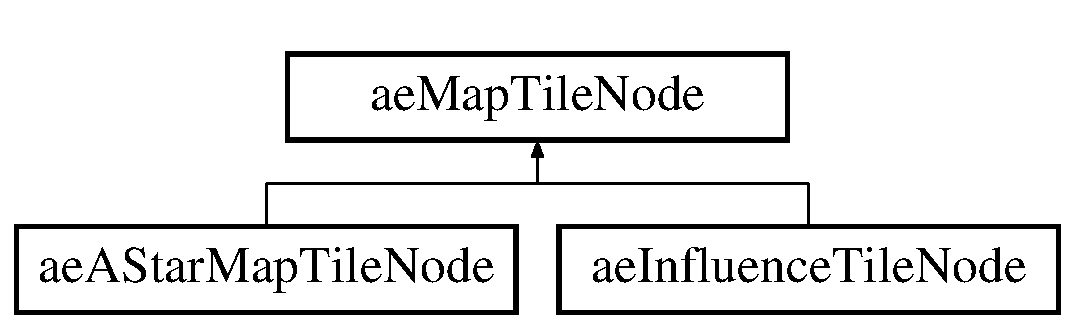
\includegraphics[height=2.000000cm]{classae_map_tile_node}
\end{center}
\end{figure}
\subsection*{Public Member Functions}
\begin{DoxyCompactItemize}
\item 
{\bfseries ae\+Map\+Tile\+Node} (const int32 x, const int32 y, \hyperlink{classae_map_tile_node}{ae\+Map\+Tile\+Node} $\ast$parent, const bool visited, const int32 cost)\hypertarget{classae_map_tile_node_a476b29ad543cb1c001f4117da3bc04c9}{}\label{classae_map_tile_node_a476b29ad543cb1c001f4117da3bc04c9}

\item 
{\bfseries ae\+Map\+Tile\+Node} (const \hyperlink{classae_map_tile_node}{ae\+Map\+Tile\+Node} \&copy)\hypertarget{classae_map_tile_node_a7f77906699c1648ec41acce383044fcf}{}\label{classae_map_tile_node_a7f77906699c1648ec41acce383044fcf}

\item 
virtual \hyperlink{classae_map_tile_node}{ae\+Map\+Tile\+Node} \& {\bfseries operator=} (const \hyperlink{classae_map_tile_node}{ae\+Map\+Tile\+Node} \&rhs)\hypertarget{classae_map_tile_node_a8e092f03e147e59a721f418ac01bda79}{}\label{classae_map_tile_node_a8e092f03e147e59a721f418ac01bda79}

\item 
virtual bool {\bfseries operator==} (const \hyperlink{classae_map_tile_node}{ae\+Map\+Tile\+Node} \&rhs)\hypertarget{classae_map_tile_node_a5c968db5b5580d8c0b6be554418d9c30}{}\label{classae_map_tile_node_a5c968db5b5580d8c0b6be554418d9c30}

\item 
virtual bool {\bfseries operator$<$} (const \hyperlink{classae_map_tile_node}{ae\+Map\+Tile\+Node} \&rhs)\hypertarget{classae_map_tile_node_a73cd36e1fa79e1486bdfc3480c27711d}{}\label{classae_map_tile_node_a73cd36e1fa79e1486bdfc3480c27711d}

\item 
virtual bool {\bfseries operator$>$} (const \hyperlink{classae_map_tile_node}{ae\+Map\+Tile\+Node} \&rhs)\hypertarget{classae_map_tile_node_af2f48e1ef88b17c57d420a4cc565ccde}{}\label{classae_map_tile_node_af2f48e1ef88b17c57d420a4cc565ccde}

\item 
void {\bfseries Set\+Parent} (\hyperlink{classae_map_tile_node}{ae\+Map\+Tile\+Node} $\ast$parent)\hypertarget{classae_map_tile_node_aa4cb85eddd3946b7f3bf2908487391bd}{}\label{classae_map_tile_node_aa4cb85eddd3946b7f3bf2908487391bd}

\item 
void {\bfseries Set\+Visited} (const bool visited)\hypertarget{classae_map_tile_node_a3d795d12dfca638d69352ee31265e7ef}{}\label{classae_map_tile_node_a3d795d12dfca638d69352ee31265e7ef}

\item 
bool {\bfseries Get\+Visited} () const \hypertarget{classae_map_tile_node_a243689baa5ecef13f46f8ed3e797e772}{}\label{classae_map_tile_node_a243689baa5ecef13f46f8ed3e797e772}

\item 
virtual void {\bfseries Set\+Cost} (const \hyperlink{namespaceae_core_a862bc39eb87cfabca273f49e2a920129}{int32} cost)\hypertarget{classae_map_tile_node_a076c949c338a01d53d6496c375fadd9b}{}\label{classae_map_tile_node_a076c949c338a01d53d6496c375fadd9b}

\item 
virtual \hyperlink{namespaceae_core_a862bc39eb87cfabca273f49e2a920129}{int32} {\bfseries Get\+Cost} () const \hypertarget{classae_map_tile_node_a31b806242d821f4ce62174094858b659}{}\label{classae_map_tile_node_a31b806242d821f4ce62174094858b659}

\item 
bool {\bfseries Equals} (const \hyperlink{classae_map_tile_node}{ae\+Map\+Tile\+Node} \&rhs) const \hypertarget{classae_map_tile_node_a472307fed8aac17c894eabbccdee6e9e}{}\label{classae_map_tile_node_a472307fed8aac17c894eabbccdee6e9e}

\end{DoxyCompactItemize}
\subsection*{Public Attributes}
\begin{DoxyCompactItemize}
\item 
int32 {\bfseries m\+\_\+x}\hypertarget{classae_map_tile_node_a570f1e8a2a2b66e90f514935ec155d76}{}\label{classae_map_tile_node_a570f1e8a2a2b66e90f514935ec155d76}

\item 
int32 {\bfseries m\+\_\+y}\hypertarget{classae_map_tile_node_acd2a5abd41dff0834271fa9c83c7e857}{}\label{classae_map_tile_node_acd2a5abd41dff0834271fa9c83c7e857}

\item 
int32 {\bfseries m\+\_\+cost}\hypertarget{classae_map_tile_node_a63625c9702e0380960791a7033803e33}{}\label{classae_map_tile_node_a63625c9702e0380960791a7033803e33}

\item 
bool {\bfseries m\+\_\+visited}\hypertarget{classae_map_tile_node_af0ad3f1b0e3cb5309323ee59c60c668e}{}\label{classae_map_tile_node_af0ad3f1b0e3cb5309323ee59c60c668e}

\item 
\hyperlink{classae_map_tile_node}{ae\+Map\+Tile\+Node} $\ast$ {\bfseries m\+\_\+parent}\hypertarget{classae_map_tile_node_ad53935b025ed63a79b92d14578ec257e}{}\label{classae_map_tile_node_ad53935b025ed63a79b92d14578ec257e}

\end{DoxyCompactItemize}


The documentation for this class was generated from the following files\+:\begin{DoxyCompactItemize}
\item 
C\+:/\+Users/\+Alvaro Estrada/\+Documents/\+Visual Studio 2015/\+Projects/\+R\+T\+S\+\_\+\+A\+E/\+R\+T\+S\+\_\+\+A\+E/\+Game/\hyperlink{_map_tile_node_8h}{Map\+Tile\+Node.\+h}\item 
C\+:/\+Users/\+Alvaro Estrada/\+Documents/\+Visual Studio 2015/\+Projects/\+R\+T\+S\+\_\+\+A\+E/\+R\+T\+S\+\_\+\+A\+E/\+Game/\hyperlink{_map_tile_node_8cpp}{Map\+Tile\+Node.\+cpp}\end{DoxyCompactItemize}

\hypertarget{structae_core_1_1ae_matrix2}{}\section{ae\+Core\+:\+:ae\+Matrix2 Struct Reference}
\label{structae_core_1_1ae_matrix2}\index{ae\+Core\+::ae\+Matrix2@{ae\+Core\+::ae\+Matrix2}}


This structure is a 2x2 matrix of float values. This is an old structure, better use \hyperlink{structae_core_1_1ae_matrix3}{ae\+Matrix3}.  




{\ttfamily \#include $<$Matrix2.\+h$>$}

\subsection*{Public Member Functions}
\begin{DoxyCompactItemize}
\item 
\hyperlink{structae_core_1_1ae_matrix2_af2acf066a442a3982b2e93371d209b6e}{ae\+Matrix2} (const \hyperlink{structae_core_1_1ae_matrix2}{ae\+Matrix2} \&Reference\+Matrix)\hypertarget{structae_core_1_1ae_matrix2_af2acf066a442a3982b2e93371d209b6e}{}\label{structae_core_1_1ae_matrix2_af2acf066a442a3982b2e93371d209b6e}

\begin{DoxyCompactList}\small\item\em Create a copy of another 2x2 matrix. \end{DoxyCompactList}\item 
\hyperlink{structae_core_1_1ae_matrix2_ac1c8c301a89c48d6e26a5946a3dc505c}{ae\+Matrix2} (float Matrix\+Position00, float Matrix\+Position01, float Matrix\+Position10, float Matrix\+Position11)\hypertarget{structae_core_1_1ae_matrix2_ac1c8c301a89c48d6e26a5946a3dc505c}{}\label{structae_core_1_1ae_matrix2_ac1c8c301a89c48d6e26a5946a3dc505c}

\begin{DoxyCompactList}\small\item\em Create a new Matrix from given values. \end{DoxyCompactList}\item 
void {\bfseries Set\+Col} (\hyperlink{structae_core_1_1ae_vector2}{ae\+Vector2} \&Reference\+Vector, int Column\+Number)\hypertarget{structae_core_1_1ae_matrix2_a34813a9838b2d43ef443a36b376c9976}{}\label{structae_core_1_1ae_matrix2_a34813a9838b2d43ef443a36b376c9976}

\item 
void {\bfseries Set\+Row} (\hyperlink{structae_core_1_1ae_vector2}{ae\+Vector2} \&Reference\+Vector, int Row\+Number)\hypertarget{structae_core_1_1ae_matrix2_a66a2d4cbb0ee8a8acadcfa9347e63d18}{}\label{structae_core_1_1ae_matrix2_a66a2d4cbb0ee8a8acadcfa9347e63d18}

\item 
\hyperlink{structae_core_1_1ae_vector2}{ae\+Vector2} {\bfseries Get\+Col} (int Column\+Number)\hypertarget{structae_core_1_1ae_matrix2_a3be78323909e8f086d66ca072f66d812}{}\label{structae_core_1_1ae_matrix2_a3be78323909e8f086d66ca072f66d812}

\item 
\hyperlink{structae_core_1_1ae_vector2}{ae\+Vector2} {\bfseries Get\+Row} (int Row\+Number)\hypertarget{structae_core_1_1ae_matrix2_a0a5c4c5dca7ebbde54d5e6bce0419590}{}\label{structae_core_1_1ae_matrix2_a0a5c4c5dca7ebbde54d5e6bce0419590}

\item 
\hyperlink{structae_core_1_1ae_vector2}{ae\+Vector2} {\bfseries operator$\ast$} (\hyperlink{structae_core_1_1ae_vector2}{ae\+Vector2} \&Reference\+Vector)\hypertarget{structae_core_1_1ae_matrix2_ae124ebeac38325ddba24a37645197738}{}\label{structae_core_1_1ae_matrix2_ae124ebeac38325ddba24a37645197738}

\item 
\hyperlink{structae_core_1_1ae_matrix2}{ae\+Matrix2} {\bfseries operator+} (\hyperlink{structae_core_1_1ae_matrix2}{ae\+Matrix2} \&Reference\+Matrix)\hypertarget{structae_core_1_1ae_matrix2_ac09005b77405c2f7b46eebfbe9443b54}{}\label{structae_core_1_1ae_matrix2_ac09005b77405c2f7b46eebfbe9443b54}

\item 
\hyperlink{structae_core_1_1ae_matrix2}{ae\+Matrix2} {\bfseries operator-\/} (\hyperlink{structae_core_1_1ae_matrix2}{ae\+Matrix2} \&Reference\+Matrix)\hypertarget{structae_core_1_1ae_matrix2_a28bee7681e71622ceb75d9fb69b3b03a}{}\label{structae_core_1_1ae_matrix2_a28bee7681e71622ceb75d9fb69b3b03a}

\item 
\hyperlink{structae_core_1_1ae_matrix2}{ae\+Matrix2} {\bfseries operator$\ast$} (\hyperlink{structae_core_1_1ae_matrix2}{ae\+Matrix2} \&Reference\+Matrix)\hypertarget{structae_core_1_1ae_matrix2_a4d662772692aefaed63e17fd3becabb8}{}\label{structae_core_1_1ae_matrix2_a4d662772692aefaed63e17fd3becabb8}

\item 
\hyperlink{structae_core_1_1ae_matrix2}{ae\+Matrix2} {\bfseries operator$\ast$} (float Coefficient)\hypertarget{structae_core_1_1ae_matrix2_a42de223400e3460a8697cd62e4b1c6db}{}\label{structae_core_1_1ae_matrix2_a42de223400e3460a8697cd62e4b1c6db}

\item 
\hyperlink{structae_core_1_1ae_matrix2}{ae\+Matrix2} {\bfseries operator/} (float Divider)\hypertarget{structae_core_1_1ae_matrix2_ab60bd3dfd41328acd24acf32d8f40fa6}{}\label{structae_core_1_1ae_matrix2_ab60bd3dfd41328acd24acf32d8f40fa6}

\item 
\hyperlink{structae_core_1_1ae_matrix2}{ae\+Matrix2} {\bfseries operator+=} (\hyperlink{structae_core_1_1ae_matrix2}{ae\+Matrix2} \&Reference\+Matrix)\hypertarget{structae_core_1_1ae_matrix2_a43e34364f048b2bd3a4d00338c0db356}{}\label{structae_core_1_1ae_matrix2_a43e34364f048b2bd3a4d00338c0db356}

\item 
\hyperlink{structae_core_1_1ae_matrix2}{ae\+Matrix2} {\bfseries operator-\/=} (\hyperlink{structae_core_1_1ae_matrix2}{ae\+Matrix2} \&Reference\+Matrix)\hypertarget{structae_core_1_1ae_matrix2_a3368043b77baaf3f491660cd818b82df}{}\label{structae_core_1_1ae_matrix2_a3368043b77baaf3f491660cd818b82df}

\item 
\hyperlink{structae_core_1_1ae_matrix2}{ae\+Matrix2} {\bfseries operator$\ast$=} (\hyperlink{structae_core_1_1ae_matrix2}{ae\+Matrix2} \&Reference\+Matrix)\hypertarget{structae_core_1_1ae_matrix2_a49c2400ea3a1b62d0f2ccdef5400e376}{}\label{structae_core_1_1ae_matrix2_a49c2400ea3a1b62d0f2ccdef5400e376}

\item 
\hyperlink{structae_core_1_1ae_matrix2}{ae\+Matrix2} {\bfseries operator$\ast$=} (float Coefficient)\hypertarget{structae_core_1_1ae_matrix2_aae38bf8d29d05ea29ab2ae097aa252f1}{}\label{structae_core_1_1ae_matrix2_aae38bf8d29d05ea29ab2ae097aa252f1}

\item 
\hyperlink{structae_core_1_1ae_matrix2}{ae\+Matrix2} {\bfseries operator/=} (float Divider)\hypertarget{structae_core_1_1ae_matrix2_adf3da5cd905b9300ca95e57722482cba}{}\label{structae_core_1_1ae_matrix2_adf3da5cd905b9300ca95e57722482cba}

\item 
float \hyperlink{structae_core_1_1ae_matrix2_a21754da48aa2b7d62b3671df9ad857d9}{Det} ()
\begin{DoxyCompactList}\small\item\em Obtains the determinant of this matrix. \end{DoxyCompactList}\item 
\hyperlink{structae_core_1_1ae_vector2}{ae\+Vector2} \hyperlink{structae_core_1_1ae_matrix2_a56a2ed15734c12e6758e24e5b99e320b}{Cramer} (\hyperlink{structae_core_1_1ae_vector2}{ae\+Vector2} \&Reference\+Vector)
\begin{DoxyCompactList}\small\item\em Uses Cramer\textquotesingle{}s rule for the solution of an equation system. \end{DoxyCompactList}\item 
\hyperlink{structae_core_1_1ae_matrix2}{ae\+Matrix2} \hyperlink{structae_core_1_1ae_matrix2_adb256aaa0254d5d5a39b15922459617c}{Transpose} ()
\begin{DoxyCompactList}\small\item\em Obtain the transposed matrix of this matrix. \end{DoxyCompactList}\item 
\hyperlink{structae_core_1_1ae_matrix2}{ae\+Matrix2} \hyperlink{structae_core_1_1ae_matrix2_afc3bfb3199e6250d07b87e2753c72ffe}{Cofactor} ()
\begin{DoxyCompactList}\small\item\em Obtains the cofactor matrix of this matrix. \end{DoxyCompactList}\item 
\hyperlink{structae_core_1_1ae_matrix2}{ae\+Matrix2} \hyperlink{structae_core_1_1ae_matrix2_a9562f29192a261d3bb08d638d01a8668}{Adjunct} ()
\begin{DoxyCompactList}\small\item\em Obtains the adjunct matrix of this matrix. \end{DoxyCompactList}\item 
\hyperlink{structae_core_1_1ae_matrix2}{ae\+Matrix2} \hyperlink{structae_core_1_1ae_matrix2_a190c5cf6cd89327845f57be611243c13}{Inverse} ()
\begin{DoxyCompactList}\small\item\em Obtains the inverse matrix of this matrix. \end{DoxyCompactList}\end{DoxyCompactItemize}
\subsection*{Static Public Member Functions}
\begin{DoxyCompactItemize}
\item 
static \hyperlink{structae_core_1_1ae_matrix2}{ae\+Matrix2} \hyperlink{structae_core_1_1ae_matrix2_aa314cad424dcb8d7ee122f1397fca4fb}{Zero} ()
\begin{DoxyCompactList}\small\item\em Returns an empty matrix. \end{DoxyCompactList}\item 
static \hyperlink{structae_core_1_1ae_matrix2}{ae\+Matrix2} \hyperlink{structae_core_1_1ae_matrix2_af67a31c083ff59452091bc8527b3e81e}{Identity} ()
\begin{DoxyCompactList}\small\item\em Returns an identity matrix. \end{DoxyCompactList}\item 
static \hyperlink{structae_core_1_1ae_matrix2}{ae\+Matrix2} \hyperlink{structae_core_1_1ae_matrix2_af6b83fc1bdf500046cc1dc179f7e7bd7}{Scaling\+Matrix} (\hyperlink{structae_core_1_1ae_vector2}{ae\+Vector2} \&Scale\+Vector)
\begin{DoxyCompactList}\small\item\em Creates a scaling matrix from a vector. \end{DoxyCompactList}\item 
static \hyperlink{structae_core_1_1ae_matrix2}{ae\+Matrix2} \hyperlink{structae_core_1_1ae_matrix2_a1a3437ad1dbb0a69570ab587e23205e8}{Scaling\+Matrix} (float Scale\+Factor)
\begin{DoxyCompactList}\small\item\em Creates a scaling matrix from a scale factor. \end{DoxyCompactList}\item 
static \hyperlink{structae_core_1_1ae_matrix2}{ae\+Matrix2} \hyperlink{structae_core_1_1ae_matrix2_afbdb5f8de5d189d44d91ede806a06d1f}{Rotation\+Matrix} (float Radians\+Of\+Rotation)
\begin{DoxyCompactList}\small\item\em Creates a rotation matrix from an angle. \end{DoxyCompactList}\item 
static \hyperlink{structae_core_1_1ae_vector2}{ae\+Vector2} \hyperlink{structae_core_1_1ae_matrix2_aa6547cd8f9036d87ce781ce83510e307}{Rotate} (float Radians\+Of\+Rotation, \hyperlink{structae_core_1_1ae_vector2}{ae\+Vector2} \&Vector\+To\+Rotate)
\begin{DoxyCompactList}\small\item\em Returns the rotated vector given an angle. \end{DoxyCompactList}\item 
static \hyperlink{structae_core_1_1ae_vector2}{ae\+Vector2} \hyperlink{structae_core_1_1ae_matrix2_a00ac01f6801c84661e859a2115645122}{Rotate} (\hyperlink{structae_core_1_1ae_vector2}{ae\+Vector2} \&Vector\+To\+Rotate, \hyperlink{structae_core_1_1ae_vector2}{ae\+Vector2} \&Vector\+Adding\+Rotation)
\begin{DoxyCompactList}\small\item\em Returns the rotated vector given another vector. \end{DoxyCompactList}\item 
static \hyperlink{structae_core_1_1ae_vector2}{ae\+Vector2} \hyperlink{structae_core_1_1ae_matrix2_a3f2cbb0c29b87b04e1c421932b8c0127}{Homogeneous\+Transformation} (\hyperlink{structae_core_1_1ae_vector2}{ae\+Vector2} \&Vector\+To\+Transform, \hyperlink{structae_core_1_1ae_vector2}{ae\+Vector2} \&Translation\+Vector, \hyperlink{structae_core_1_1ae_vector2}{ae\+Vector2} \&Scale\+Vector, \hyperlink{structae_core_1_1ae_vector2}{ae\+Vector2} \&Vector\+Adding\+Rotation)
\begin{DoxyCompactList}\small\item\em Homogeneous transformation. \end{DoxyCompactList}\item 
static \hyperlink{structae_core_1_1ae_vector2}{ae\+Vector2} \hyperlink{structae_core_1_1ae_matrix2_a60802ab5a75638359d1c482a1a14d460}{Homogeneous\+Transformation} (\hyperlink{structae_core_1_1ae_vector2}{ae\+Vector2} \&Vector\+To\+Transform, \hyperlink{structae_core_1_1ae_vector2}{ae\+Vector2} \&Translation\+Vector, \hyperlink{structae_core_1_1ae_vector2}{ae\+Vector2} \&Scale\+Vector, float Radians\+Of\+Rotation)
\begin{DoxyCompactList}\small\item\em Homogeneous transformation. \end{DoxyCompactList}\item 
static \hyperlink{structae_core_1_1ae_vector2}{ae\+Vector2} \hyperlink{structae_core_1_1ae_matrix2_a9f0399f9481315d8e1e096b8b8ed6b85}{Homogeneous\+Transformation} (\hyperlink{structae_core_1_1ae_vector2}{ae\+Vector2} \&Vector\+To\+Transform, \hyperlink{structae_core_1_1ae_vector2}{ae\+Vector2} \&Translation\+Vector, float Scale\+Factor, float Radians\+Of\+Rotation)
\begin{DoxyCompactList}\small\item\em Homogeneous transformation. \end{DoxyCompactList}\end{DoxyCompactItemize}
\subsection*{Public Attributes}
\begin{DoxyCompactItemize}
\item 
float {\bfseries m\+\_\+f00}\hypertarget{structae_core_1_1ae_matrix2_ac600acbe39b321caf26e3c5eda50e38e}{}\label{structae_core_1_1ae_matrix2_ac600acbe39b321caf26e3c5eda50e38e}

\item 
float {\bfseries m\+\_\+f01}\hypertarget{structae_core_1_1ae_matrix2_a04061d9d9a48a117a41c66aa51402ae9}{}\label{structae_core_1_1ae_matrix2_a04061d9d9a48a117a41c66aa51402ae9}

\item 
float {\bfseries m\+\_\+f10}\hypertarget{structae_core_1_1ae_matrix2_a9d02f2b413e90a2e4af9f37a1ac30303}{}\label{structae_core_1_1ae_matrix2_a9d02f2b413e90a2e4af9f37a1ac30303}

\item 
float {\bfseries m\+\_\+f11}\hypertarget{structae_core_1_1ae_matrix2_ae0a2ec187b94745c2a3fea9ad7db5ce8}{}\label{structae_core_1_1ae_matrix2_ae0a2ec187b94745c2a3fea9ad7db5ce8}

\end{DoxyCompactItemize}


\subsection{Detailed Description}
This structure is a 2x2 matrix of float values. This is an old structure, better use \hyperlink{structae_core_1_1ae_matrix3}{ae\+Matrix3}. 

\begin{DoxyAuthor}{Author}
Alvaro Estrada 
\end{DoxyAuthor}
\begin{DoxyDate}{Date}
14/05/2016 
\end{DoxyDate}


\subsection{Member Function Documentation}
\index{ae\+Core\+::ae\+Matrix2@{ae\+Core\+::ae\+Matrix2}!Adjunct@{Adjunct}}
\index{Adjunct@{Adjunct}!ae\+Core\+::ae\+Matrix2@{ae\+Core\+::ae\+Matrix2}}
\subsubsection[{\texorpdfstring{Adjunct()}{Adjunct()}}]{\setlength{\rightskip}{0pt plus 5cm}{\bf ae\+Matrix2} ae\+Core\+::ae\+Matrix2\+::\+Adjunct (
\begin{DoxyParamCaption}
{}
\end{DoxyParamCaption}
)}\hypertarget{structae_core_1_1ae_matrix2_a9562f29192a261d3bb08d638d01a8668}{}\label{structae_core_1_1ae_matrix2_a9562f29192a261d3bb08d638d01a8668}


Obtains the adjunct matrix of this matrix. 

\begin{DoxyReturn}{Returns}
A \hyperlink{structae_core_1_1ae_matrix2}{ae\+Matrix2}. 
\end{DoxyReturn}
\index{ae\+Core\+::ae\+Matrix2@{ae\+Core\+::ae\+Matrix2}!Cofactor@{Cofactor}}
\index{Cofactor@{Cofactor}!ae\+Core\+::ae\+Matrix2@{ae\+Core\+::ae\+Matrix2}}
\subsubsection[{\texorpdfstring{Cofactor()}{Cofactor()}}]{\setlength{\rightskip}{0pt plus 5cm}{\bf ae\+Matrix2} ae\+Core\+::ae\+Matrix2\+::\+Cofactor (
\begin{DoxyParamCaption}
{}
\end{DoxyParamCaption}
)}\hypertarget{structae_core_1_1ae_matrix2_afc3bfb3199e6250d07b87e2753c72ffe}{}\label{structae_core_1_1ae_matrix2_afc3bfb3199e6250d07b87e2753c72ffe}


Obtains the cofactor matrix of this matrix. 

\begin{DoxyReturn}{Returns}
A \hyperlink{structae_core_1_1ae_matrix2}{ae\+Matrix2}. 
\end{DoxyReturn}
\index{ae\+Core\+::ae\+Matrix2@{ae\+Core\+::ae\+Matrix2}!Cramer@{Cramer}}
\index{Cramer@{Cramer}!ae\+Core\+::ae\+Matrix2@{ae\+Core\+::ae\+Matrix2}}
\subsubsection[{\texorpdfstring{Cramer(ae\+Vector2 \&\+Reference\+Vector)}{Cramer(aeVector2 &ReferenceVector)}}]{\setlength{\rightskip}{0pt plus 5cm}{\bf ae\+Vector2} ae\+Core\+::ae\+Matrix2\+::\+Cramer (
\begin{DoxyParamCaption}
\item[{{\bf ae\+Vector2} \&}]{Reference\+Vector}
\end{DoxyParamCaption}
)}\hypertarget{structae_core_1_1ae_matrix2_a56a2ed15734c12e6758e24e5b99e320b}{}\label{structae_core_1_1ae_matrix2_a56a2ed15734c12e6758e24e5b99e320b}


Uses Cramer\textquotesingle{}s rule for the solution of an equation system. 


\begin{DoxyParams}[1]{Parameters}
\mbox{\tt in,out}  & {\em Reference\+Vector} & The reference vector.\\
\hline
\end{DoxyParams}
\begin{DoxyReturn}{Returns}
A \hyperlink{structae_core_1_1ae_vector2}{ae\+Vector2}. 
\end{DoxyReturn}
\index{ae\+Core\+::ae\+Matrix2@{ae\+Core\+::ae\+Matrix2}!Det@{Det}}
\index{Det@{Det}!ae\+Core\+::ae\+Matrix2@{ae\+Core\+::ae\+Matrix2}}
\subsubsection[{\texorpdfstring{Det()}{Det()}}]{\setlength{\rightskip}{0pt plus 5cm}float ae\+Core\+::ae\+Matrix2\+::\+Det (
\begin{DoxyParamCaption}
{}
\end{DoxyParamCaption}
)}\hypertarget{structae_core_1_1ae_matrix2_a21754da48aa2b7d62b3671df9ad857d9}{}\label{structae_core_1_1ae_matrix2_a21754da48aa2b7d62b3671df9ad857d9}


Obtains the determinant of this matrix. 

\begin{DoxyReturn}{Returns}
A float. 
\end{DoxyReturn}
\index{ae\+Core\+::ae\+Matrix2@{ae\+Core\+::ae\+Matrix2}!Homogeneous\+Transformation@{Homogeneous\+Transformation}}
\index{Homogeneous\+Transformation@{Homogeneous\+Transformation}!ae\+Core\+::ae\+Matrix2@{ae\+Core\+::ae\+Matrix2}}
\subsubsection[{\texorpdfstring{Homogeneous\+Transformation(ae\+Vector2 \&\+Vector\+To\+Transform, ae\+Vector2 \&\+Translation\+Vector, ae\+Vector2 \&\+Scale\+Vector, ae\+Vector2 \&\+Vector\+Adding\+Rotation)}{HomogeneousTransformation(aeVector2 &VectorToTransform, aeVector2 &TranslationVector, aeVector2 &ScaleVector, aeVector2 &VectorAddingRotation)}}]{\setlength{\rightskip}{0pt plus 5cm}static {\bf ae\+Vector2} ae\+Core\+::ae\+Matrix2\+::\+Homogeneous\+Transformation (
\begin{DoxyParamCaption}
\item[{{\bf ae\+Vector2} \&}]{Vector\+To\+Transform, }
\item[{{\bf ae\+Vector2} \&}]{Translation\+Vector, }
\item[{{\bf ae\+Vector2} \&}]{Scale\+Vector, }
\item[{{\bf ae\+Vector2} \&}]{Vector\+Adding\+Rotation}
\end{DoxyParamCaption}
)\hspace{0.3cm}{\ttfamily [static]}}\hypertarget{structae_core_1_1ae_matrix2_a3f2cbb0c29b87b04e1c421932b8c0127}{}\label{structae_core_1_1ae_matrix2_a3f2cbb0c29b87b04e1c421932b8c0127}


Homogeneous transformation. 


\begin{DoxyParams}[1]{Parameters}
\mbox{\tt in,out}  & {\em Vector\+To\+Transform} & The vector to transform. \\
\hline
\mbox{\tt in,out}  & {\em Translation\+Vector} & The translation vector. \\
\hline
\mbox{\tt in,out}  & {\em Scale\+Vector} & The scale vector. \\
\hline
\mbox{\tt in,out}  & {\em Vector\+Adding\+Rotation} & The vector adding rotation.\\
\hline
\end{DoxyParams}
\begin{DoxyReturn}{Returns}
A \hyperlink{structae_core_1_1ae_vector2}{ae\+Vector2}. 
\end{DoxyReturn}
\index{ae\+Core\+::ae\+Matrix2@{ae\+Core\+::ae\+Matrix2}!Homogeneous\+Transformation@{Homogeneous\+Transformation}}
\index{Homogeneous\+Transformation@{Homogeneous\+Transformation}!ae\+Core\+::ae\+Matrix2@{ae\+Core\+::ae\+Matrix2}}
\subsubsection[{\texorpdfstring{Homogeneous\+Transformation(ae\+Vector2 \&\+Vector\+To\+Transform, ae\+Vector2 \&\+Translation\+Vector, ae\+Vector2 \&\+Scale\+Vector, float Radians\+Of\+Rotation)}{HomogeneousTransformation(aeVector2 &VectorToTransform, aeVector2 &TranslationVector, aeVector2 &ScaleVector, float RadiansOfRotation)}}]{\setlength{\rightskip}{0pt plus 5cm}static {\bf ae\+Vector2} ae\+Core\+::ae\+Matrix2\+::\+Homogeneous\+Transformation (
\begin{DoxyParamCaption}
\item[{{\bf ae\+Vector2} \&}]{Vector\+To\+Transform, }
\item[{{\bf ae\+Vector2} \&}]{Translation\+Vector, }
\item[{{\bf ae\+Vector2} \&}]{Scale\+Vector, }
\item[{float}]{Radians\+Of\+Rotation}
\end{DoxyParamCaption}
)\hspace{0.3cm}{\ttfamily [static]}}\hypertarget{structae_core_1_1ae_matrix2_a60802ab5a75638359d1c482a1a14d460}{}\label{structae_core_1_1ae_matrix2_a60802ab5a75638359d1c482a1a14d460}


Homogeneous transformation. 


\begin{DoxyParams}[1]{Parameters}
\mbox{\tt in,out}  & {\em Vector\+To\+Transform} & The vector to transform. \\
\hline
\mbox{\tt in,out}  & {\em Translation\+Vector} & The translation vector. \\
\hline
\mbox{\tt in,out}  & {\em Scale\+Vector} & The scale vector. \\
\hline
 & {\em Radians\+Of\+Rotation} & The radians of rotation.\\
\hline
\end{DoxyParams}
\begin{DoxyReturn}{Returns}
A \hyperlink{structae_core_1_1ae_vector2}{ae\+Vector2}. 
\end{DoxyReturn}
\index{ae\+Core\+::ae\+Matrix2@{ae\+Core\+::ae\+Matrix2}!Homogeneous\+Transformation@{Homogeneous\+Transformation}}
\index{Homogeneous\+Transformation@{Homogeneous\+Transformation}!ae\+Core\+::ae\+Matrix2@{ae\+Core\+::ae\+Matrix2}}
\subsubsection[{\texorpdfstring{Homogeneous\+Transformation(ae\+Vector2 \&\+Vector\+To\+Transform, ae\+Vector2 \&\+Translation\+Vector, float Scale\+Factor, float Radians\+Of\+Rotation)}{HomogeneousTransformation(aeVector2 &VectorToTransform, aeVector2 &TranslationVector, float ScaleFactor, float RadiansOfRotation)}}]{\setlength{\rightskip}{0pt plus 5cm}static {\bf ae\+Vector2} ae\+Core\+::ae\+Matrix2\+::\+Homogeneous\+Transformation (
\begin{DoxyParamCaption}
\item[{{\bf ae\+Vector2} \&}]{Vector\+To\+Transform, }
\item[{{\bf ae\+Vector2} \&}]{Translation\+Vector, }
\item[{float}]{Scale\+Factor, }
\item[{float}]{Radians\+Of\+Rotation}
\end{DoxyParamCaption}
)\hspace{0.3cm}{\ttfamily [static]}}\hypertarget{structae_core_1_1ae_matrix2_a9f0399f9481315d8e1e096b8b8ed6b85}{}\label{structae_core_1_1ae_matrix2_a9f0399f9481315d8e1e096b8b8ed6b85}


Homogeneous transformation. 


\begin{DoxyParams}[1]{Parameters}
\mbox{\tt in,out}  & {\em Vector\+To\+Transform} & The vector to transform. \\
\hline
\mbox{\tt in,out}  & {\em Translation\+Vector} & The translation vector. \\
\hline
 & {\em Scale\+Factor} & The scale factor. \\
\hline
 & {\em Radians\+Of\+Rotation} & The radians of rotation.\\
\hline
\end{DoxyParams}
\begin{DoxyReturn}{Returns}
A \hyperlink{structae_core_1_1ae_vector2}{ae\+Vector2}. 
\end{DoxyReturn}
\index{ae\+Core\+::ae\+Matrix2@{ae\+Core\+::ae\+Matrix2}!Identity@{Identity}}
\index{Identity@{Identity}!ae\+Core\+::ae\+Matrix2@{ae\+Core\+::ae\+Matrix2}}
\subsubsection[{\texorpdfstring{Identity()}{Identity()}}]{\setlength{\rightskip}{0pt plus 5cm}static {\bf ae\+Matrix2} ae\+Core\+::ae\+Matrix2\+::\+Identity (
\begin{DoxyParamCaption}
{}
\end{DoxyParamCaption}
)\hspace{0.3cm}{\ttfamily [inline]}, {\ttfamily [static]}}\hypertarget{structae_core_1_1ae_matrix2_af67a31c083ff59452091bc8527b3e81e}{}\label{structae_core_1_1ae_matrix2_af67a31c083ff59452091bc8527b3e81e}


Returns an identity matrix. 

\begin{DoxyReturn}{Returns}
A \hyperlink{structae_core_1_1ae_matrix3}{ae\+Matrix3}. 
\end{DoxyReturn}
\index{ae\+Core\+::ae\+Matrix2@{ae\+Core\+::ae\+Matrix2}!Inverse@{Inverse}}
\index{Inverse@{Inverse}!ae\+Core\+::ae\+Matrix2@{ae\+Core\+::ae\+Matrix2}}
\subsubsection[{\texorpdfstring{Inverse()}{Inverse()}}]{\setlength{\rightskip}{0pt plus 5cm}{\bf ae\+Matrix2} ae\+Core\+::ae\+Matrix2\+::\+Inverse (
\begin{DoxyParamCaption}
{}
\end{DoxyParamCaption}
)}\hypertarget{structae_core_1_1ae_matrix2_a190c5cf6cd89327845f57be611243c13}{}\label{structae_core_1_1ae_matrix2_a190c5cf6cd89327845f57be611243c13}


Obtains the inverse matrix of this matrix. 

\begin{DoxyReturn}{Returns}
A \hyperlink{structae_core_1_1ae_matrix2}{ae\+Matrix2}. 
\end{DoxyReturn}
\index{ae\+Core\+::ae\+Matrix2@{ae\+Core\+::ae\+Matrix2}!Rotate@{Rotate}}
\index{Rotate@{Rotate}!ae\+Core\+::ae\+Matrix2@{ae\+Core\+::ae\+Matrix2}}
\subsubsection[{\texorpdfstring{Rotate(float Radians\+Of\+Rotation, ae\+Vector2 \&\+Vector\+To\+Rotate)}{Rotate(float RadiansOfRotation, aeVector2 &VectorToRotate)}}]{\setlength{\rightskip}{0pt plus 5cm}static {\bf ae\+Vector2} ae\+Core\+::ae\+Matrix2\+::\+Rotate (
\begin{DoxyParamCaption}
\item[{float}]{Radians\+Of\+Rotation, }
\item[{{\bf ae\+Vector2} \&}]{Vector\+To\+Rotate}
\end{DoxyParamCaption}
)\hspace{0.3cm}{\ttfamily [static]}}\hypertarget{structae_core_1_1ae_matrix2_aa6547cd8f9036d87ce781ce83510e307}{}\label{structae_core_1_1ae_matrix2_aa6547cd8f9036d87ce781ce83510e307}


Returns the rotated vector given an angle. 


\begin{DoxyParams}[1]{Parameters}
 & {\em Radians\+Of\+Rotation} & The radians of rotation. \\
\hline
\mbox{\tt in,out}  & {\em Vector\+To\+Rotate} & The vector to rotate.\\
\hline
\end{DoxyParams}
\begin{DoxyReturn}{Returns}
A \hyperlink{structae_core_1_1ae_vector2}{ae\+Vector2}. 
\end{DoxyReturn}
\index{ae\+Core\+::ae\+Matrix2@{ae\+Core\+::ae\+Matrix2}!Rotate@{Rotate}}
\index{Rotate@{Rotate}!ae\+Core\+::ae\+Matrix2@{ae\+Core\+::ae\+Matrix2}}
\subsubsection[{\texorpdfstring{Rotate(ae\+Vector2 \&\+Vector\+To\+Rotate, ae\+Vector2 \&\+Vector\+Adding\+Rotation)}{Rotate(aeVector2 &VectorToRotate, aeVector2 &VectorAddingRotation)}}]{\setlength{\rightskip}{0pt plus 5cm}static {\bf ae\+Vector2} ae\+Core\+::ae\+Matrix2\+::\+Rotate (
\begin{DoxyParamCaption}
\item[{{\bf ae\+Vector2} \&}]{Vector\+To\+Rotate, }
\item[{{\bf ae\+Vector2} \&}]{Vector\+Adding\+Rotation}
\end{DoxyParamCaption}
)\hspace{0.3cm}{\ttfamily [static]}}\hypertarget{structae_core_1_1ae_matrix2_a00ac01f6801c84661e859a2115645122}{}\label{structae_core_1_1ae_matrix2_a00ac01f6801c84661e859a2115645122}


Returns the rotated vector given another vector. 


\begin{DoxyParams}[1]{Parameters}
\mbox{\tt in,out}  & {\em Vector\+To\+Rotate} & The vector to rotate. \\
\hline
\mbox{\tt in,out}  & {\em Vector\+Adding\+Rotation} & The vector adding rotation.\\
\hline
\end{DoxyParams}
\begin{DoxyReturn}{Returns}
A \hyperlink{structae_core_1_1ae_vector2}{ae\+Vector2}. 
\end{DoxyReturn}
\index{ae\+Core\+::ae\+Matrix2@{ae\+Core\+::ae\+Matrix2}!Rotation\+Matrix@{Rotation\+Matrix}}
\index{Rotation\+Matrix@{Rotation\+Matrix}!ae\+Core\+::ae\+Matrix2@{ae\+Core\+::ae\+Matrix2}}
\subsubsection[{\texorpdfstring{Rotation\+Matrix(float Radians\+Of\+Rotation)}{RotationMatrix(float RadiansOfRotation)}}]{\setlength{\rightskip}{0pt plus 5cm}static {\bf ae\+Matrix2} ae\+Core\+::ae\+Matrix2\+::\+Rotation\+Matrix (
\begin{DoxyParamCaption}
\item[{float}]{Radians\+Of\+Rotation}
\end{DoxyParamCaption}
)\hspace{0.3cm}{\ttfamily [static]}}\hypertarget{structae_core_1_1ae_matrix2_afbdb5f8de5d189d44d91ede806a06d1f}{}\label{structae_core_1_1ae_matrix2_afbdb5f8de5d189d44d91ede806a06d1f}


Creates a rotation matrix from an angle. 


\begin{DoxyParams}{Parameters}
{\em Radians\+Of\+Rotation} & The radians of rotation.\\
\hline
\end{DoxyParams}
\begin{DoxyReturn}{Returns}
A \hyperlink{structae_core_1_1ae_matrix2}{ae\+Matrix2}. 
\end{DoxyReturn}
\index{ae\+Core\+::ae\+Matrix2@{ae\+Core\+::ae\+Matrix2}!Scaling\+Matrix@{Scaling\+Matrix}}
\index{Scaling\+Matrix@{Scaling\+Matrix}!ae\+Core\+::ae\+Matrix2@{ae\+Core\+::ae\+Matrix2}}
\subsubsection[{\texorpdfstring{Scaling\+Matrix(ae\+Vector2 \&\+Scale\+Vector)}{ScalingMatrix(aeVector2 &ScaleVector)}}]{\setlength{\rightskip}{0pt plus 5cm}static {\bf ae\+Matrix2} ae\+Core\+::ae\+Matrix2\+::\+Scaling\+Matrix (
\begin{DoxyParamCaption}
\item[{{\bf ae\+Vector2} \&}]{Scale\+Vector}
\end{DoxyParamCaption}
)\hspace{0.3cm}{\ttfamily [static]}}\hypertarget{structae_core_1_1ae_matrix2_af6b83fc1bdf500046cc1dc179f7e7bd7}{}\label{structae_core_1_1ae_matrix2_af6b83fc1bdf500046cc1dc179f7e7bd7}


Creates a scaling matrix from a vector. 


\begin{DoxyParams}[1]{Parameters}
\mbox{\tt in,out}  & {\em Scale\+Vector} & The scale vector.\\
\hline
\end{DoxyParams}
\begin{DoxyReturn}{Returns}
A \hyperlink{structae_core_1_1ae_matrix2}{ae\+Matrix2}. 
\end{DoxyReturn}
\index{ae\+Core\+::ae\+Matrix2@{ae\+Core\+::ae\+Matrix2}!Scaling\+Matrix@{Scaling\+Matrix}}
\index{Scaling\+Matrix@{Scaling\+Matrix}!ae\+Core\+::ae\+Matrix2@{ae\+Core\+::ae\+Matrix2}}
\subsubsection[{\texorpdfstring{Scaling\+Matrix(float Scale\+Factor)}{ScalingMatrix(float ScaleFactor)}}]{\setlength{\rightskip}{0pt plus 5cm}static {\bf ae\+Matrix2} ae\+Core\+::ae\+Matrix2\+::\+Scaling\+Matrix (
\begin{DoxyParamCaption}
\item[{float}]{Scale\+Factor}
\end{DoxyParamCaption}
)\hspace{0.3cm}{\ttfamily [static]}}\hypertarget{structae_core_1_1ae_matrix2_a1a3437ad1dbb0a69570ab587e23205e8}{}\label{structae_core_1_1ae_matrix2_a1a3437ad1dbb0a69570ab587e23205e8}


Creates a scaling matrix from a scale factor. 


\begin{DoxyParams}{Parameters}
{\em Scale\+Factor} & The scale factor.\\
\hline
\end{DoxyParams}
\begin{DoxyReturn}{Returns}
A \hyperlink{structae_core_1_1ae_matrix2}{ae\+Matrix2}. 
\end{DoxyReturn}
\index{ae\+Core\+::ae\+Matrix2@{ae\+Core\+::ae\+Matrix2}!Transpose@{Transpose}}
\index{Transpose@{Transpose}!ae\+Core\+::ae\+Matrix2@{ae\+Core\+::ae\+Matrix2}}
\subsubsection[{\texorpdfstring{Transpose()}{Transpose()}}]{\setlength{\rightskip}{0pt plus 5cm}{\bf ae\+Matrix2} ae\+Core\+::ae\+Matrix2\+::\+Transpose (
\begin{DoxyParamCaption}
{}
\end{DoxyParamCaption}
)}\hypertarget{structae_core_1_1ae_matrix2_adb256aaa0254d5d5a39b15922459617c}{}\label{structae_core_1_1ae_matrix2_adb256aaa0254d5d5a39b15922459617c}


Obtain the transposed matrix of this matrix. 

\begin{DoxyReturn}{Returns}
A \hyperlink{structae_core_1_1ae_matrix2}{ae\+Matrix2}. 
\end{DoxyReturn}
\index{ae\+Core\+::ae\+Matrix2@{ae\+Core\+::ae\+Matrix2}!Zero@{Zero}}
\index{Zero@{Zero}!ae\+Core\+::ae\+Matrix2@{ae\+Core\+::ae\+Matrix2}}
\subsubsection[{\texorpdfstring{Zero()}{Zero()}}]{\setlength{\rightskip}{0pt plus 5cm}static {\bf ae\+Matrix2} ae\+Core\+::ae\+Matrix2\+::\+Zero (
\begin{DoxyParamCaption}
{}
\end{DoxyParamCaption}
)\hspace{0.3cm}{\ttfamily [inline]}, {\ttfamily [static]}}\hypertarget{structae_core_1_1ae_matrix2_aa314cad424dcb8d7ee122f1397fca4fb}{}\label{structae_core_1_1ae_matrix2_aa314cad424dcb8d7ee122f1397fca4fb}


Returns an empty matrix. 

\begin{DoxyReturn}{Returns}
A \hyperlink{structae_core_1_1ae_matrix3}{ae\+Matrix3}. 
\end{DoxyReturn}


The documentation for this struct was generated from the following files\+:\begin{DoxyCompactItemize}
\item 
C\+:/\+Users/\+Alvaro Estrada/\+Documents/\+Visual Studio 2015/\+Projects/\+R\+T\+S\+\_\+\+A\+E/ae\+Core/\+Math/Matrix2.\+h\item 
C\+:/\+Users/\+Alvaro Estrada/\+Documents/\+Visual Studio 2015/\+Projects/\+R\+T\+S\+\_\+\+A\+E/ae\+Core/\+Math/Matrix2.\+cpp\end{DoxyCompactItemize}

\hypertarget{structae_core_1_1ae_matrix3}{}\section{ae\+Core\+:\+:ae\+Matrix3 Struct Reference}
\label{structae_core_1_1ae_matrix3}\index{ae\+Core\+::ae\+Matrix3@{ae\+Core\+::ae\+Matrix3}}


This structure is a 3x3 matrix of float values.  




{\ttfamily \#include $<$Matrix3.\+h$>$}

\subsection*{Public Member Functions}
\begin{DoxyCompactItemize}
\item 
\hyperlink{structae_core_1_1ae_matrix3_ae6db4e959d0cbfbfe741c3c6a479dcae}{ae\+Matrix3} (const \hyperlink{structae_core_1_1ae_matrix3}{ae\+Matrix3} \&Reference\+Matrix)\hypertarget{structae_core_1_1ae_matrix3_ae6db4e959d0cbfbfe741c3c6a479dcae}{}\label{structae_core_1_1ae_matrix3_ae6db4e959d0cbfbfe741c3c6a479dcae}

\begin{DoxyCompactList}\small\item\em Create a copy of another 2x2 matrix. \end{DoxyCompactList}\item 
\hyperlink{structae_core_1_1ae_matrix3_ab2f2c69ccb0dfad3daa9baa444fccd00}{ae\+Matrix3} (float \+\_\+00, float \+\_\+01=0, float \+\_\+02=0, float \+\_\+10=0, float \+\_\+11=1, float \+\_\+12=0, float \+\_\+20=0, float \+\_\+21=0, float \+\_\+22=1)\hypertarget{structae_core_1_1ae_matrix3_ab2f2c69ccb0dfad3daa9baa444fccd00}{}\label{structae_core_1_1ae_matrix3_ab2f2c69ccb0dfad3daa9baa444fccd00}

\begin{DoxyCompactList}\small\item\em Create a new Matrix from given values. \end{DoxyCompactList}\item 
void {\bfseries Set\+Col} (\hyperlink{structae_core_1_1ae_vector3}{ae\+Vector3} \&Reference\+Vector, int Column\+Number)\hypertarget{structae_core_1_1ae_matrix3_a2b0dd3c1ceb10107c8871e33adde3f47}{}\label{structae_core_1_1ae_matrix3_a2b0dd3c1ceb10107c8871e33adde3f47}

\item 
void {\bfseries Set\+Row} (\hyperlink{structae_core_1_1ae_vector3}{ae\+Vector3} \&Reference\+Vector, int Row\+Number)\hypertarget{structae_core_1_1ae_matrix3_a0a3df9088e467cd240b12b92421bcb62}{}\label{structae_core_1_1ae_matrix3_a0a3df9088e467cd240b12b92421bcb62}

\item 
\hyperlink{structae_core_1_1ae_vector3}{ae\+Vector3} {\bfseries Get\+Col} (int Column\+Number)\hypertarget{structae_core_1_1ae_matrix3_aec1281aaae26af580cacfa86d6fc06a9}{}\label{structae_core_1_1ae_matrix3_aec1281aaae26af580cacfa86d6fc06a9}

\item 
\hyperlink{structae_core_1_1ae_vector3}{ae\+Vector3} {\bfseries Get\+Row} (int Row\+Number)\hypertarget{structae_core_1_1ae_matrix3_a6ca53eed248289f7d6775cd0521de62b}{}\label{structae_core_1_1ae_matrix3_a6ca53eed248289f7d6775cd0521de62b}

\item 
\hyperlink{structae_core_1_1ae_vector3}{ae\+Vector3} {\bfseries operator$\ast$} (\hyperlink{structae_core_1_1ae_vector3}{ae\+Vector3} \&Reference\+Vector)\hypertarget{structae_core_1_1ae_matrix3_a75869d5a5f5c32d4172d7b2e945c241f}{}\label{structae_core_1_1ae_matrix3_a75869d5a5f5c32d4172d7b2e945c241f}

\item 
\hyperlink{structae_core_1_1ae_matrix3}{ae\+Matrix3} {\bfseries operator+} (\hyperlink{structae_core_1_1ae_matrix3}{ae\+Matrix3} \&Reference\+Matrix)\hypertarget{structae_core_1_1ae_matrix3_a0a15766b9f4fb71772aeafc5be6b6af4}{}\label{structae_core_1_1ae_matrix3_a0a15766b9f4fb71772aeafc5be6b6af4}

\item 
\hyperlink{structae_core_1_1ae_matrix3}{ae\+Matrix3} {\bfseries operator-\/} (\hyperlink{structae_core_1_1ae_matrix3}{ae\+Matrix3} \&Reference\+Matrix)\hypertarget{structae_core_1_1ae_matrix3_a322077f4ede52405f119de321eac9c97}{}\label{structae_core_1_1ae_matrix3_a322077f4ede52405f119de321eac9c97}

\item 
\hyperlink{structae_core_1_1ae_matrix3}{ae\+Matrix3} {\bfseries operator$\ast$} (\hyperlink{structae_core_1_1ae_matrix3}{ae\+Matrix3} \&Reference\+Matrix)\hypertarget{structae_core_1_1ae_matrix3_ab83a8b194e37159e5d3be7f82e946711}{}\label{structae_core_1_1ae_matrix3_ab83a8b194e37159e5d3be7f82e946711}

\item 
\hyperlink{structae_core_1_1ae_matrix3}{ae\+Matrix3} {\bfseries operator$\ast$} (float Coefficient)\hypertarget{structae_core_1_1ae_matrix3_a31bc65cdd5a33c2a2174331e59343fa3}{}\label{structae_core_1_1ae_matrix3_a31bc65cdd5a33c2a2174331e59343fa3}

\item 
\hyperlink{structae_core_1_1ae_matrix3}{ae\+Matrix3} {\bfseries operator/} (float Divider)\hypertarget{structae_core_1_1ae_matrix3_a703743917ec8ae4a8c7731de507c0d9f}{}\label{structae_core_1_1ae_matrix3_a703743917ec8ae4a8c7731de507c0d9f}

\item 
\hyperlink{structae_core_1_1ae_matrix3}{ae\+Matrix3} {\bfseries operator+=} (\hyperlink{structae_core_1_1ae_matrix3}{ae\+Matrix3} \&Reference\+Matrix)\hypertarget{structae_core_1_1ae_matrix3_a5c02f34881c81411422c7151c086396c}{}\label{structae_core_1_1ae_matrix3_a5c02f34881c81411422c7151c086396c}

\item 
\hyperlink{structae_core_1_1ae_matrix3}{ae\+Matrix3} {\bfseries operator-\/=} (\hyperlink{structae_core_1_1ae_matrix3}{ae\+Matrix3} \&Reference\+Matrix)\hypertarget{structae_core_1_1ae_matrix3_a75389cc09bd49677dc68c40277f76709}{}\label{structae_core_1_1ae_matrix3_a75389cc09bd49677dc68c40277f76709}

\item 
\hyperlink{structae_core_1_1ae_matrix3}{ae\+Matrix3} {\bfseries operator$\ast$=} (\hyperlink{structae_core_1_1ae_matrix3}{ae\+Matrix3} \&Reference\+Matrix)\hypertarget{structae_core_1_1ae_matrix3_ab12b5138f5e8064817b255b145aac965}{}\label{structae_core_1_1ae_matrix3_ab12b5138f5e8064817b255b145aac965}

\item 
\hyperlink{structae_core_1_1ae_matrix3}{ae\+Matrix3} {\bfseries operator$\ast$=} (float Coefficient)\hypertarget{structae_core_1_1ae_matrix3_ac67bc97a44c94e67b67483adcda15662}{}\label{structae_core_1_1ae_matrix3_ac67bc97a44c94e67b67483adcda15662}

\item 
\hyperlink{structae_core_1_1ae_matrix3}{ae\+Matrix3} {\bfseries operator/=} (float Divider)\hypertarget{structae_core_1_1ae_matrix3_a33932f8767e11c82ce5f7b836bacba96}{}\label{structae_core_1_1ae_matrix3_a33932f8767e11c82ce5f7b836bacba96}

\item 
float \hyperlink{structae_core_1_1ae_matrix3_ae4c2757efb47769dbeb24e65db2ceea4}{Det} ()
\begin{DoxyCompactList}\small\item\em Obtains the determinant of this matrix. \end{DoxyCompactList}\item 
\hyperlink{structae_core_1_1ae_vector3}{ae\+Vector3} \hyperlink{structae_core_1_1ae_matrix3_ae2c041d8f63ffe9790c8ffe7fa07a39a}{Cramer} (\hyperlink{structae_core_1_1ae_vector3}{ae\+Vector3} \&Reference\+Vector)
\begin{DoxyCompactList}\small\item\em Uses Cramer\textquotesingle{}s rule for the solution of an equation system. \end{DoxyCompactList}\item 
\hyperlink{structae_core_1_1ae_matrix3}{ae\+Matrix3} \hyperlink{structae_core_1_1ae_matrix3_a05be8551f23506aa3eb5856e9a84b0dd}{Transpose} ()
\begin{DoxyCompactList}\small\item\em Obtain the transposed matrix of this matrix. \end{DoxyCompactList}\item 
\hyperlink{structae_core_1_1ae_matrix3}{ae\+Matrix3} \hyperlink{structae_core_1_1ae_matrix3_aff995dc5d1f6fea6c9fb79901e552806}{Cofactor} ()
\begin{DoxyCompactList}\small\item\em Obtains the cofactor matrix of this matrix. \end{DoxyCompactList}\item 
\hyperlink{structae_core_1_1ae_matrix3}{ae\+Matrix3} \hyperlink{structae_core_1_1ae_matrix3_a5a5977b809c70665b8ae74ec2478b0ab}{Adjunct} ()
\begin{DoxyCompactList}\small\item\em Obtains the adjunct matrix of this matrix. \end{DoxyCompactList}\item 
\hyperlink{structae_core_1_1ae_matrix3}{ae\+Matrix3} \hyperlink{structae_core_1_1ae_matrix3_a3cd375176637d7da7262a7627eac1cdd}{Inverse} ()
\begin{DoxyCompactList}\small\item\em Obtains the transposed matrix of this matrix. \end{DoxyCompactList}\end{DoxyCompactItemize}
\subsection*{Static Public Member Functions}
\begin{DoxyCompactItemize}
\item 
static \hyperlink{structae_core_1_1ae_matrix3}{ae\+Matrix3} \hyperlink{structae_core_1_1ae_matrix3_a029f4b68fa7e2901ed65fb0d64e64a18}{Zero} ()
\begin{DoxyCompactList}\small\item\em Returns an empty matrix. \end{DoxyCompactList}\item 
static \hyperlink{structae_core_1_1ae_matrix3}{ae\+Matrix3} \hyperlink{structae_core_1_1ae_matrix3_ab6a48e3b08b761ac11aedcdd706fd846}{Identity} ()
\begin{DoxyCompactList}\small\item\em Returns an identity matrix. \end{DoxyCompactList}\item 
static \hyperlink{structae_core_1_1ae_matrix3}{ae\+Matrix3} \hyperlink{structae_core_1_1ae_matrix3_a334964d8152fe8e1b65efcb60d7c8846}{Translation\+Matrix} (\hyperlink{structae_core_1_1ae_vector3}{ae\+Vector3} \&Translation\+Vector)
\begin{DoxyCompactList}\small\item\em Creates a translation matrix from a vector. \end{DoxyCompactList}\item 
static \hyperlink{structae_core_1_1ae_matrix3}{ae\+Matrix3} \hyperlink{structae_core_1_1ae_matrix3_a46258dc1190c86544355a8dcb1685105}{Translation\+Matrix} (\hyperlink{structae_core_1_1ae_vector2}{ae\+Vector2} \&Translation\+Vector)
\begin{DoxyCompactList}\small\item\em Creates a translation matrix from a vector. \end{DoxyCompactList}\item 
static \hyperlink{structae_core_1_1ae_matrix3}{ae\+Matrix3} \hyperlink{structae_core_1_1ae_matrix3_aceb7b649f9d26fdcac597d231d8054a8}{Translation\+Matrix} (float X, float Y)
\begin{DoxyCompactList}\small\item\em Creates a translation matrix from 2 parameters. \end{DoxyCompactList}\item 
static \hyperlink{structae_core_1_1ae_matrix3}{ae\+Matrix3} \hyperlink{structae_core_1_1ae_matrix3_abaa5cfdac45bc7ce9a61ede3a55891b3}{Scaling\+Matrix} (\hyperlink{structae_core_1_1ae_vector3}{ae\+Vector3} \&Scale\+Vector)
\begin{DoxyCompactList}\small\item\em Creates a scaling matrix from a vector. \end{DoxyCompactList}\item 
static \hyperlink{structae_core_1_1ae_matrix3}{ae\+Matrix3} \hyperlink{structae_core_1_1ae_matrix3_a4321c0bb6cdb696d83f44226e2a99324}{Scaling\+Matrix} (\hyperlink{structae_core_1_1ae_vector2}{ae\+Vector2} \&Scale\+Vector)
\begin{DoxyCompactList}\small\item\em Creates a scaling matrix from a vector. \end{DoxyCompactList}\item 
static \hyperlink{structae_core_1_1ae_matrix3}{ae\+Matrix3} \hyperlink{structae_core_1_1ae_matrix3_ac4c3497053ca4456e6ae86e3583ee3fa}{Scaling\+Matrix} (float Scale\+Factor)
\begin{DoxyCompactList}\small\item\em Creates a scaling matrix from a scale factor. \end{DoxyCompactList}\item 
static \hyperlink{structae_core_1_1ae_matrix3}{ae\+Matrix3} \hyperlink{structae_core_1_1ae_matrix3_a02fe9054e3f64428feeadea3973364f6}{Scaling\+Matrix} (float x, float y)
\begin{DoxyCompactList}\small\item\em Creates a scaling matrix from 2 scale factors. \end{DoxyCompactList}\item 
static \hyperlink{structae_core_1_1ae_matrix3}{ae\+Matrix3} \hyperlink{structae_core_1_1ae_matrix3_a9034112410e48d7eda9b692b869fe817}{RotationX} (float theta)
\begin{DoxyCompactList}\small\item\em Creates a rotation matrix from an angle to rotate on the X axis. \end{DoxyCompactList}\item 
static \hyperlink{structae_core_1_1ae_matrix3}{ae\+Matrix3} \hyperlink{structae_core_1_1ae_matrix3_a204bdb33efb9ad0e790bb046f354e021}{RotationY} (float theta)
\begin{DoxyCompactList}\small\item\em Creates a rotation matrix from an angle to rotate on the Y axis. \end{DoxyCompactList}\item 
static \hyperlink{structae_core_1_1ae_matrix3}{ae\+Matrix3} \hyperlink{structae_core_1_1ae_matrix3_a1bdcfb36a05ecc7abe36351777c5c789}{RotationZ} (float theta)
\begin{DoxyCompactList}\small\item\em Creates a rotation matrix from an angle to rotate on the Z axis. \end{DoxyCompactList}\end{DoxyCompactItemize}
\subsection*{Public Attributes}
\begin{DoxyCompactItemize}
\item 
\begin{tabbing}
xx\=xx\=xx\=xx\=xx\=xx\=xx\=xx\=xx\=\kill
union \{\\
\>struct \{\\
\>\>float {\bfseries m\_f00}\\
\>\>float {\bfseries m\_f01}\\
\>\>float {\bfseries m\_f02}\\
\>\>float {\bfseries m\_f10}\\
\>\>float {\bfseries m\_f11}\\
\>\>float {\bfseries m\_f12}\\
\>\>float {\bfseries m\_f20}\\
\>\>float {\bfseries m\_f21}\\
\>\>float {\bfseries m\_f22}\\
\>\} \hypertarget{unionae_core_1_1ae_matrix3_1_1_0D18_ab58290075c4ed32c535331fe616e26ab}{}\label{unionae_core_1_1ae_matrix3_1_1_0D18_ab58290075c4ed32c535331fe616e26ab}
\\
\>\>\>{\em A structure meant to save the matrix as individual values. }\\
\>float \hyperlink{structae_core_1_1ae_matrix3_ab9d323ce0dcb61f884fb57b6beabca41}{v} \mbox{[}9\mbox{]}\\
\>\>\>{\em A 9 times float array. }\\
\>float \hyperlink{structae_core_1_1ae_matrix3_ae173adde44ccb0c95e59894f60cbb4ec}{m} \mbox{[}3\mbox{]}\mbox{[}3\mbox{]}\\
\>\>\>{\em A 3x3 float array. }\\
\}; \hypertarget{structae_core_1_1ae_matrix3_a12e362ddd217f4268441d31750b88774}{}\label{structae_core_1_1ae_matrix3_a12e362ddd217f4268441d31750b88774}
\\

\end{tabbing}\begin{DoxyCompactList}\small\item\em Is the union between individual values and their array and matrix form. \end{DoxyCompactList}\end{DoxyCompactItemize}


\subsection{Detailed Description}
This structure is a 3x3 matrix of float values. 

\begin{DoxyAuthor}{Author}
Alvaro Estrada 
\end{DoxyAuthor}
\begin{DoxyDate}{Date}
14/05/2016 
\end{DoxyDate}


\subsection{Member Function Documentation}
\index{ae\+Core\+::ae\+Matrix3@{ae\+Core\+::ae\+Matrix3}!Adjunct@{Adjunct}}
\index{Adjunct@{Adjunct}!ae\+Core\+::ae\+Matrix3@{ae\+Core\+::ae\+Matrix3}}
\subsubsection[{\texorpdfstring{Adjunct()}{Adjunct()}}]{\setlength{\rightskip}{0pt plus 5cm}{\bf ae\+Matrix3} ae\+Core\+::ae\+Matrix3\+::\+Adjunct (
\begin{DoxyParamCaption}
{}
\end{DoxyParamCaption}
)}\hypertarget{structae_core_1_1ae_matrix3_a5a5977b809c70665b8ae74ec2478b0ab}{}\label{structae_core_1_1ae_matrix3_a5a5977b809c70665b8ae74ec2478b0ab}


Obtains the adjunct matrix of this matrix. 

\begin{DoxyReturn}{Returns}
A \hyperlink{structae_core_1_1ae_matrix3}{ae\+Matrix3}. 
\end{DoxyReturn}
\index{ae\+Core\+::ae\+Matrix3@{ae\+Core\+::ae\+Matrix3}!Cofactor@{Cofactor}}
\index{Cofactor@{Cofactor}!ae\+Core\+::ae\+Matrix3@{ae\+Core\+::ae\+Matrix3}}
\subsubsection[{\texorpdfstring{Cofactor()}{Cofactor()}}]{\setlength{\rightskip}{0pt plus 5cm}{\bf ae\+Matrix3} ae\+Core\+::ae\+Matrix3\+::\+Cofactor (
\begin{DoxyParamCaption}
{}
\end{DoxyParamCaption}
)}\hypertarget{structae_core_1_1ae_matrix3_aff995dc5d1f6fea6c9fb79901e552806}{}\label{structae_core_1_1ae_matrix3_aff995dc5d1f6fea6c9fb79901e552806}


Obtains the cofactor matrix of this matrix. 

\begin{DoxyReturn}{Returns}
A \hyperlink{structae_core_1_1ae_matrix3}{ae\+Matrix3}. 
\end{DoxyReturn}
\index{ae\+Core\+::ae\+Matrix3@{ae\+Core\+::ae\+Matrix3}!Cramer@{Cramer}}
\index{Cramer@{Cramer}!ae\+Core\+::ae\+Matrix3@{ae\+Core\+::ae\+Matrix3}}
\subsubsection[{\texorpdfstring{Cramer(ae\+Vector3 \&\+Reference\+Vector)}{Cramer(aeVector3 &ReferenceVector)}}]{\setlength{\rightskip}{0pt plus 5cm}{\bf ae\+Vector3} ae\+Core\+::ae\+Matrix3\+::\+Cramer (
\begin{DoxyParamCaption}
\item[{{\bf ae\+Vector3} \&}]{Reference\+Vector}
\end{DoxyParamCaption}
)}\hypertarget{structae_core_1_1ae_matrix3_ae2c041d8f63ffe9790c8ffe7fa07a39a}{}\label{structae_core_1_1ae_matrix3_ae2c041d8f63ffe9790c8ffe7fa07a39a}


Uses Cramer\textquotesingle{}s rule for the solution of an equation system. 


\begin{DoxyParams}[1]{Parameters}
\mbox{\tt in,out}  & {\em Reference\+Vector} & The reference vector.\\
\hline
\end{DoxyParams}
\begin{DoxyReturn}{Returns}
A \hyperlink{structae_core_1_1ae_vector3}{ae\+Vector3}. 
\end{DoxyReturn}
\index{ae\+Core\+::ae\+Matrix3@{ae\+Core\+::ae\+Matrix3}!Det@{Det}}
\index{Det@{Det}!ae\+Core\+::ae\+Matrix3@{ae\+Core\+::ae\+Matrix3}}
\subsubsection[{\texorpdfstring{Det()}{Det()}}]{\setlength{\rightskip}{0pt plus 5cm}float ae\+Core\+::ae\+Matrix3\+::\+Det (
\begin{DoxyParamCaption}
{}
\end{DoxyParamCaption}
)}\hypertarget{structae_core_1_1ae_matrix3_ae4c2757efb47769dbeb24e65db2ceea4}{}\label{structae_core_1_1ae_matrix3_ae4c2757efb47769dbeb24e65db2ceea4}


Obtains the determinant of this matrix. 

\begin{DoxyReturn}{Returns}
A float. 
\end{DoxyReturn}
\index{ae\+Core\+::ae\+Matrix3@{ae\+Core\+::ae\+Matrix3}!Identity@{Identity}}
\index{Identity@{Identity}!ae\+Core\+::ae\+Matrix3@{ae\+Core\+::ae\+Matrix3}}
\subsubsection[{\texorpdfstring{Identity()}{Identity()}}]{\setlength{\rightskip}{0pt plus 5cm}static {\bf ae\+Matrix3} ae\+Core\+::ae\+Matrix3\+::\+Identity (
\begin{DoxyParamCaption}
{}
\end{DoxyParamCaption}
)\hspace{0.3cm}{\ttfamily [static]}}\hypertarget{structae_core_1_1ae_matrix3_ab6a48e3b08b761ac11aedcdd706fd846}{}\label{structae_core_1_1ae_matrix3_ab6a48e3b08b761ac11aedcdd706fd846}


Returns an identity matrix. 

\begin{DoxyReturn}{Returns}
A \hyperlink{structae_core_1_1ae_matrix3}{ae\+Matrix3}. 
\end{DoxyReturn}
\index{ae\+Core\+::ae\+Matrix3@{ae\+Core\+::ae\+Matrix3}!Inverse@{Inverse}}
\index{Inverse@{Inverse}!ae\+Core\+::ae\+Matrix3@{ae\+Core\+::ae\+Matrix3}}
\subsubsection[{\texorpdfstring{Inverse()}{Inverse()}}]{\setlength{\rightskip}{0pt plus 5cm}{\bf ae\+Matrix3} ae\+Core\+::ae\+Matrix3\+::\+Inverse (
\begin{DoxyParamCaption}
{}
\end{DoxyParamCaption}
)}\hypertarget{structae_core_1_1ae_matrix3_a3cd375176637d7da7262a7627eac1cdd}{}\label{structae_core_1_1ae_matrix3_a3cd375176637d7da7262a7627eac1cdd}


Obtains the transposed matrix of this matrix. 

\begin{DoxyReturn}{Returns}
A \hyperlink{structae_core_1_1ae_matrix3}{ae\+Matrix3}. 
\end{DoxyReturn}
\index{ae\+Core\+::ae\+Matrix3@{ae\+Core\+::ae\+Matrix3}!RotationX@{RotationX}}
\index{RotationX@{RotationX}!ae\+Core\+::ae\+Matrix3@{ae\+Core\+::ae\+Matrix3}}
\subsubsection[{\texorpdfstring{Rotation\+X(float theta)}{RotationX(float theta)}}]{\setlength{\rightskip}{0pt plus 5cm}static {\bf ae\+Matrix3} ae\+Core\+::ae\+Matrix3\+::\+RotationX (
\begin{DoxyParamCaption}
\item[{float}]{theta}
\end{DoxyParamCaption}
)\hspace{0.3cm}{\ttfamily [static]}}\hypertarget{structae_core_1_1ae_matrix3_a9034112410e48d7eda9b692b869fe817}{}\label{structae_core_1_1ae_matrix3_a9034112410e48d7eda9b692b869fe817}


Creates a rotation matrix from an angle to rotate on the X axis. 


\begin{DoxyParams}{Parameters}
{\em theta} & The radians of rotation.\\
\hline
\end{DoxyParams}
\begin{DoxyReturn}{Returns}
A \hyperlink{structae_core_1_1ae_matrix3}{ae\+Matrix3}. 
\end{DoxyReturn}
\index{ae\+Core\+::ae\+Matrix3@{ae\+Core\+::ae\+Matrix3}!RotationY@{RotationY}}
\index{RotationY@{RotationY}!ae\+Core\+::ae\+Matrix3@{ae\+Core\+::ae\+Matrix3}}
\subsubsection[{\texorpdfstring{Rotation\+Y(float theta)}{RotationY(float theta)}}]{\setlength{\rightskip}{0pt plus 5cm}static {\bf ae\+Matrix3} ae\+Core\+::ae\+Matrix3\+::\+RotationY (
\begin{DoxyParamCaption}
\item[{float}]{theta}
\end{DoxyParamCaption}
)\hspace{0.3cm}{\ttfamily [static]}}\hypertarget{structae_core_1_1ae_matrix3_a204bdb33efb9ad0e790bb046f354e021}{}\label{structae_core_1_1ae_matrix3_a204bdb33efb9ad0e790bb046f354e021}


Creates a rotation matrix from an angle to rotate on the Y axis. 


\begin{DoxyParams}{Parameters}
{\em theta} & The radians of rotation.\\
\hline
\end{DoxyParams}
\begin{DoxyReturn}{Returns}
A \hyperlink{structae_core_1_1ae_matrix3}{ae\+Matrix3}. 
\end{DoxyReturn}
\index{ae\+Core\+::ae\+Matrix3@{ae\+Core\+::ae\+Matrix3}!RotationZ@{RotationZ}}
\index{RotationZ@{RotationZ}!ae\+Core\+::ae\+Matrix3@{ae\+Core\+::ae\+Matrix3}}
\subsubsection[{\texorpdfstring{Rotation\+Z(float theta)}{RotationZ(float theta)}}]{\setlength{\rightskip}{0pt plus 5cm}static {\bf ae\+Matrix3} ae\+Core\+::ae\+Matrix3\+::\+RotationZ (
\begin{DoxyParamCaption}
\item[{float}]{theta}
\end{DoxyParamCaption}
)\hspace{0.3cm}{\ttfamily [static]}}\hypertarget{structae_core_1_1ae_matrix3_a1bdcfb36a05ecc7abe36351777c5c789}{}\label{structae_core_1_1ae_matrix3_a1bdcfb36a05ecc7abe36351777c5c789}


Creates a rotation matrix from an angle to rotate on the Z axis. 


\begin{DoxyParams}{Parameters}
{\em theta} & The radians of rotation.\\
\hline
\end{DoxyParams}
\begin{DoxyReturn}{Returns}
A \hyperlink{structae_core_1_1ae_matrix3}{ae\+Matrix3}. 
\end{DoxyReturn}
\index{ae\+Core\+::ae\+Matrix3@{ae\+Core\+::ae\+Matrix3}!Scaling\+Matrix@{Scaling\+Matrix}}
\index{Scaling\+Matrix@{Scaling\+Matrix}!ae\+Core\+::ae\+Matrix3@{ae\+Core\+::ae\+Matrix3}}
\subsubsection[{\texorpdfstring{Scaling\+Matrix(ae\+Vector3 \&\+Scale\+Vector)}{ScalingMatrix(aeVector3 &ScaleVector)}}]{\setlength{\rightskip}{0pt plus 5cm}static {\bf ae\+Matrix3} ae\+Core\+::ae\+Matrix3\+::\+Scaling\+Matrix (
\begin{DoxyParamCaption}
\item[{{\bf ae\+Vector3} \&}]{Scale\+Vector}
\end{DoxyParamCaption}
)\hspace{0.3cm}{\ttfamily [static]}}\hypertarget{structae_core_1_1ae_matrix3_abaa5cfdac45bc7ce9a61ede3a55891b3}{}\label{structae_core_1_1ae_matrix3_abaa5cfdac45bc7ce9a61ede3a55891b3}


Creates a scaling matrix from a vector. 


\begin{DoxyParams}[1]{Parameters}
\mbox{\tt in,out}  & {\em Scale\+Vector} & The scale factor.\\
\hline
\end{DoxyParams}
\begin{DoxyReturn}{Returns}
A \hyperlink{structae_core_1_1ae_matrix3}{ae\+Matrix3}. 
\end{DoxyReturn}
\index{ae\+Core\+::ae\+Matrix3@{ae\+Core\+::ae\+Matrix3}!Scaling\+Matrix@{Scaling\+Matrix}}
\index{Scaling\+Matrix@{Scaling\+Matrix}!ae\+Core\+::ae\+Matrix3@{ae\+Core\+::ae\+Matrix3}}
\subsubsection[{\texorpdfstring{Scaling\+Matrix(ae\+Vector2 \&\+Scale\+Vector)}{ScalingMatrix(aeVector2 &ScaleVector)}}]{\setlength{\rightskip}{0pt plus 5cm}static {\bf ae\+Matrix3} ae\+Core\+::ae\+Matrix3\+::\+Scaling\+Matrix (
\begin{DoxyParamCaption}
\item[{{\bf ae\+Vector2} \&}]{Scale\+Vector}
\end{DoxyParamCaption}
)\hspace{0.3cm}{\ttfamily [static]}}\hypertarget{structae_core_1_1ae_matrix3_a4321c0bb6cdb696d83f44226e2a99324}{}\label{structae_core_1_1ae_matrix3_a4321c0bb6cdb696d83f44226e2a99324}


Creates a scaling matrix from a vector. 


\begin{DoxyParams}[1]{Parameters}
\mbox{\tt in,out}  & {\em Scale\+Vector} & The scale factor.\\
\hline
\end{DoxyParams}
\begin{DoxyReturn}{Returns}
A \hyperlink{structae_core_1_1ae_matrix3}{ae\+Matrix3}. 
\end{DoxyReturn}
\index{ae\+Core\+::ae\+Matrix3@{ae\+Core\+::ae\+Matrix3}!Scaling\+Matrix@{Scaling\+Matrix}}
\index{Scaling\+Matrix@{Scaling\+Matrix}!ae\+Core\+::ae\+Matrix3@{ae\+Core\+::ae\+Matrix3}}
\subsubsection[{\texorpdfstring{Scaling\+Matrix(float Scale\+Factor)}{ScalingMatrix(float ScaleFactor)}}]{\setlength{\rightskip}{0pt plus 5cm}static {\bf ae\+Matrix3} ae\+Core\+::ae\+Matrix3\+::\+Scaling\+Matrix (
\begin{DoxyParamCaption}
\item[{float}]{Scale\+Factor}
\end{DoxyParamCaption}
)\hspace{0.3cm}{\ttfamily [static]}}\hypertarget{structae_core_1_1ae_matrix3_ac4c3497053ca4456e6ae86e3583ee3fa}{}\label{structae_core_1_1ae_matrix3_ac4c3497053ca4456e6ae86e3583ee3fa}


Creates a scaling matrix from a scale factor. 


\begin{DoxyParams}{Parameters}
{\em Scale\+Factor} & The scale factor.\\
\hline
\end{DoxyParams}
\begin{DoxyReturn}{Returns}
A \hyperlink{structae_core_1_1ae_matrix3}{ae\+Matrix3}. 
\end{DoxyReturn}
\index{ae\+Core\+::ae\+Matrix3@{ae\+Core\+::ae\+Matrix3}!Scaling\+Matrix@{Scaling\+Matrix}}
\index{Scaling\+Matrix@{Scaling\+Matrix}!ae\+Core\+::ae\+Matrix3@{ae\+Core\+::ae\+Matrix3}}
\subsubsection[{\texorpdfstring{Scaling\+Matrix(float x, float y)}{ScalingMatrix(float x, float y)}}]{\setlength{\rightskip}{0pt plus 5cm}static {\bf ae\+Matrix3} ae\+Core\+::ae\+Matrix3\+::\+Scaling\+Matrix (
\begin{DoxyParamCaption}
\item[{float}]{x, }
\item[{float}]{y}
\end{DoxyParamCaption}
)\hspace{0.3cm}{\ttfamily [static]}}\hypertarget{structae_core_1_1ae_matrix3_a02fe9054e3f64428feeadea3973364f6}{}\label{structae_core_1_1ae_matrix3_a02fe9054e3f64428feeadea3973364f6}


Creates a scaling matrix from 2 scale factors. 


\begin{DoxyParams}{Parameters}
{\em x} & The x coordinate. \\
\hline
{\em y} & The y coordinate.\\
\hline
\end{DoxyParams}
\begin{DoxyReturn}{Returns}
A \hyperlink{structae_core_1_1ae_matrix3}{ae\+Matrix3}. 
\end{DoxyReturn}
\index{ae\+Core\+::ae\+Matrix3@{ae\+Core\+::ae\+Matrix3}!Translation\+Matrix@{Translation\+Matrix}}
\index{Translation\+Matrix@{Translation\+Matrix}!ae\+Core\+::ae\+Matrix3@{ae\+Core\+::ae\+Matrix3}}
\subsubsection[{\texorpdfstring{Translation\+Matrix(ae\+Vector3 \&\+Translation\+Vector)}{TranslationMatrix(aeVector3 &TranslationVector)}}]{\setlength{\rightskip}{0pt plus 5cm}static {\bf ae\+Matrix3} ae\+Core\+::ae\+Matrix3\+::\+Translation\+Matrix (
\begin{DoxyParamCaption}
\item[{{\bf ae\+Vector3} \&}]{Translation\+Vector}
\end{DoxyParamCaption}
)\hspace{0.3cm}{\ttfamily [static]}}\hypertarget{structae_core_1_1ae_matrix3_a334964d8152fe8e1b65efcb60d7c8846}{}\label{structae_core_1_1ae_matrix3_a334964d8152fe8e1b65efcb60d7c8846}


Creates a translation matrix from a vector. 


\begin{DoxyParams}[1]{Parameters}
\mbox{\tt in,out}  & {\em Translation\+Vector} & The translation vector.\\
\hline
\end{DoxyParams}
\begin{DoxyReturn}{Returns}
A \hyperlink{structae_core_1_1ae_matrix3}{ae\+Matrix3}. 
\end{DoxyReturn}
\index{ae\+Core\+::ae\+Matrix3@{ae\+Core\+::ae\+Matrix3}!Translation\+Matrix@{Translation\+Matrix}}
\index{Translation\+Matrix@{Translation\+Matrix}!ae\+Core\+::ae\+Matrix3@{ae\+Core\+::ae\+Matrix3}}
\subsubsection[{\texorpdfstring{Translation\+Matrix(ae\+Vector2 \&\+Translation\+Vector)}{TranslationMatrix(aeVector2 &TranslationVector)}}]{\setlength{\rightskip}{0pt plus 5cm}static {\bf ae\+Matrix3} ae\+Core\+::ae\+Matrix3\+::\+Translation\+Matrix (
\begin{DoxyParamCaption}
\item[{{\bf ae\+Vector2} \&}]{Translation\+Vector}
\end{DoxyParamCaption}
)\hspace{0.3cm}{\ttfamily [static]}}\hypertarget{structae_core_1_1ae_matrix3_a46258dc1190c86544355a8dcb1685105}{}\label{structae_core_1_1ae_matrix3_a46258dc1190c86544355a8dcb1685105}


Creates a translation matrix from a vector. 


\begin{DoxyParams}[1]{Parameters}
\mbox{\tt in,out}  & {\em Translation\+Vector} & The translation vector.\\
\hline
\end{DoxyParams}
\begin{DoxyReturn}{Returns}
A \hyperlink{structae_core_1_1ae_matrix3}{ae\+Matrix3}. 
\end{DoxyReturn}
\index{ae\+Core\+::ae\+Matrix3@{ae\+Core\+::ae\+Matrix3}!Translation\+Matrix@{Translation\+Matrix}}
\index{Translation\+Matrix@{Translation\+Matrix}!ae\+Core\+::ae\+Matrix3@{ae\+Core\+::ae\+Matrix3}}
\subsubsection[{\texorpdfstring{Translation\+Matrix(float X, float Y)}{TranslationMatrix(float X, float Y)}}]{\setlength{\rightskip}{0pt plus 5cm}static {\bf ae\+Matrix3} ae\+Core\+::ae\+Matrix3\+::\+Translation\+Matrix (
\begin{DoxyParamCaption}
\item[{float}]{X, }
\item[{float}]{Y}
\end{DoxyParamCaption}
)\hspace{0.3cm}{\ttfamily [static]}}\hypertarget{structae_core_1_1ae_matrix3_aceb7b649f9d26fdcac597d231d8054a8}{}\label{structae_core_1_1ae_matrix3_aceb7b649f9d26fdcac597d231d8054a8}


Creates a translation matrix from 2 parameters. 


\begin{DoxyParams}{Parameters}
{\em X} & The X coordinate. \\
\hline
{\em Y} & The Y coordinate.\\
\hline
\end{DoxyParams}
\begin{DoxyReturn}{Returns}
A \hyperlink{structae_core_1_1ae_matrix3}{ae\+Matrix3}. 
\end{DoxyReturn}
\index{ae\+Core\+::ae\+Matrix3@{ae\+Core\+::ae\+Matrix3}!Transpose@{Transpose}}
\index{Transpose@{Transpose}!ae\+Core\+::ae\+Matrix3@{ae\+Core\+::ae\+Matrix3}}
\subsubsection[{\texorpdfstring{Transpose()}{Transpose()}}]{\setlength{\rightskip}{0pt plus 5cm}{\bf ae\+Matrix3} ae\+Core\+::ae\+Matrix3\+::\+Transpose (
\begin{DoxyParamCaption}
{}
\end{DoxyParamCaption}
)}\hypertarget{structae_core_1_1ae_matrix3_a05be8551f23506aa3eb5856e9a84b0dd}{}\label{structae_core_1_1ae_matrix3_a05be8551f23506aa3eb5856e9a84b0dd}


Obtain the transposed matrix of this matrix. 

\begin{DoxyReturn}{Returns}
A \hyperlink{structae_core_1_1ae_matrix3}{ae\+Matrix3}. 
\end{DoxyReturn}
\index{ae\+Core\+::ae\+Matrix3@{ae\+Core\+::ae\+Matrix3}!Zero@{Zero}}
\index{Zero@{Zero}!ae\+Core\+::ae\+Matrix3@{ae\+Core\+::ae\+Matrix3}}
\subsubsection[{\texorpdfstring{Zero()}{Zero()}}]{\setlength{\rightskip}{0pt plus 5cm}static {\bf ae\+Matrix3} ae\+Core\+::ae\+Matrix3\+::\+Zero (
\begin{DoxyParamCaption}
{}
\end{DoxyParamCaption}
)\hspace{0.3cm}{\ttfamily [static]}}\hypertarget{structae_core_1_1ae_matrix3_a029f4b68fa7e2901ed65fb0d64e64a18}{}\label{structae_core_1_1ae_matrix3_a029f4b68fa7e2901ed65fb0d64e64a18}


Returns an empty matrix. 

\begin{DoxyReturn}{Returns}
A \hyperlink{structae_core_1_1ae_matrix3}{ae\+Matrix3}. 
\end{DoxyReturn}


The documentation for this struct was generated from the following files\+:\begin{DoxyCompactItemize}
\item 
C\+:/\+Users/\+Alvaro Estrada/\+Documents/\+Visual Studio 2015/\+Projects/\+R\+T\+S\+\_\+\+A\+E/ae\+Core/\+Math/Matrix3.\+h\item 
C\+:/\+Users/\+Alvaro Estrada/\+Documents/\+Visual Studio 2015/\+Projects/\+R\+T\+S\+\_\+\+A\+E/ae\+Core/\+Math/Matrix3.\+cpp\end{DoxyCompactItemize}

\hypertarget{structae_core_1_1ae_matrix4}{}\section{ae\+Core\+:\+:ae\+Matrix4 Struct Reference}
\label{structae_core_1_1ae_matrix4}\index{ae\+Core\+::ae\+Matrix4@{ae\+Core\+::ae\+Matrix4}}


This structure is a 4x4 matrix of float values.  




{\ttfamily \#include $<$Matrix4.\+h$>$}

\subsection*{Public Member Functions}
\begin{DoxyCompactItemize}
\item 
{\bfseries ae\+Matrix4} (const \hyperlink{structae_core_1_1ae_matrix4}{ae\+Matrix4} \&M)\hypertarget{structae_core_1_1ae_matrix4_ab6c8b90c1535b8bdae036e0f8665331d}{}\label{structae_core_1_1ae_matrix4_ab6c8b90c1535b8bdae036e0f8665331d}

\item 
{\bfseries ae\+Matrix4} (float \+\_\+00, float \+\_\+01=0, float \+\_\+02=0, float \+\_\+03=0, float \+\_\+10=0, float \+\_\+11=1, float \+\_\+12=0, float \+\_\+13=0, float \+\_\+20=0, float \+\_\+21=0, float \+\_\+22=1, float \+\_\+23=0, float \+\_\+30=0, float \+\_\+31=0, float \+\_\+32=0, float \+\_\+33=1)\hypertarget{structae_core_1_1ae_matrix4_a67c01cd6e4a132d837cd60ab95e8242d}{}\label{structae_core_1_1ae_matrix4_a67c01cd6e4a132d837cd60ab95e8242d}

\item 
void {\bfseries Set\+Col} (\hyperlink{structae_core_1_1ae_vector4}{ae\+Vector4} \&V, int n\+Col)\hypertarget{structae_core_1_1ae_matrix4_a8e97ad8c4de58ac761efd86fe62fcb5e}{}\label{structae_core_1_1ae_matrix4_a8e97ad8c4de58ac761efd86fe62fcb5e}

\item 
void {\bfseries Set\+Row} (\hyperlink{structae_core_1_1ae_vector4}{ae\+Vector4} \&V, int n\+Row)\hypertarget{structae_core_1_1ae_matrix4_ab7d0bad2bff73aa05cc3e7a10bf22874}{}\label{structae_core_1_1ae_matrix4_ab7d0bad2bff73aa05cc3e7a10bf22874}

\item 
\hyperlink{structae_core_1_1ae_vector4}{ae\+Vector4} {\bfseries Get\+Col} (int n\+Col)\hypertarget{structae_core_1_1ae_matrix4_a93d98eaaa7471eb5d7d7178d1f783a3d}{}\label{structae_core_1_1ae_matrix4_a93d98eaaa7471eb5d7d7178d1f783a3d}

\item 
\hyperlink{structae_core_1_1ae_vector4}{ae\+Vector4} {\bfseries Get\+Row} (int n\+Row)\hypertarget{structae_core_1_1ae_matrix4_adad8e2b60dbc3762e4bd541e64514d50}{}\label{structae_core_1_1ae_matrix4_adad8e2b60dbc3762e4bd541e64514d50}

\item 
\hyperlink{structae_core_1_1ae_matrix4}{ae\+Matrix4} {\bfseries operator+} (\hyperlink{structae_core_1_1ae_matrix4}{ae\+Matrix4} \&M)\hypertarget{structae_core_1_1ae_matrix4_a22fcc8fa65a592194939c8c97743d6e1}{}\label{structae_core_1_1ae_matrix4_a22fcc8fa65a592194939c8c97743d6e1}

\item 
\hyperlink{structae_core_1_1ae_matrix4}{ae\+Matrix4} {\bfseries operator-\/} (\hyperlink{structae_core_1_1ae_matrix4}{ae\+Matrix4} \&M)\hypertarget{structae_core_1_1ae_matrix4_a1b3853423831cf6510571a58310108f9}{}\label{structae_core_1_1ae_matrix4_a1b3853423831cf6510571a58310108f9}

\item 
\hyperlink{structae_core_1_1ae_matrix4}{ae\+Matrix4} {\bfseries operator$\ast$} (\hyperlink{structae_core_1_1ae_matrix4}{ae\+Matrix4} \&M)\hypertarget{structae_core_1_1ae_matrix4_a22023495ddd808bbb48dec691962d3f1}{}\label{structae_core_1_1ae_matrix4_a22023495ddd808bbb48dec691962d3f1}

\item 
\hyperlink{structae_core_1_1ae_matrix4}{ae\+Matrix4} {\bfseries operator$\ast$} (float s)\hypertarget{structae_core_1_1ae_matrix4_aecc208c6b607daa925b1603cbf976478}{}\label{structae_core_1_1ae_matrix4_aecc208c6b607daa925b1603cbf976478}

\item 
\hyperlink{structae_core_1_1ae_matrix4}{ae\+Matrix4} {\bfseries operator/} (float s)\hypertarget{structae_core_1_1ae_matrix4_a83b741e8a57c1986febd12f5f76c1feb}{}\label{structae_core_1_1ae_matrix4_a83b741e8a57c1986febd12f5f76c1feb}

\item 
\hyperlink{structae_core_1_1ae_vector4}{ae\+Vector4} {\bfseries operator$\ast$} (\hyperlink{structae_core_1_1ae_vector4}{ae\+Vector4} \&V)\hypertarget{structae_core_1_1ae_matrix4_a6c5fd05bf420a28067dc8cefd4be0455}{}\label{structae_core_1_1ae_matrix4_a6c5fd05bf420a28067dc8cefd4be0455}

\item 
\hyperlink{structae_core_1_1ae_matrix4}{ae\+Matrix4} \& {\bfseries operator+=} (\hyperlink{structae_core_1_1ae_matrix4}{ae\+Matrix4} \&A)\hypertarget{structae_core_1_1ae_matrix4_ac64d5bd76271a5976f3ac4ae5f7743cc}{}\label{structae_core_1_1ae_matrix4_ac64d5bd76271a5976f3ac4ae5f7743cc}

\item 
\hyperlink{structae_core_1_1ae_matrix4}{ae\+Matrix4} \& {\bfseries operator-\/=} (\hyperlink{structae_core_1_1ae_matrix4}{ae\+Matrix4} \&A)\hypertarget{structae_core_1_1ae_matrix4_ad71244f9aa9d38348048eb3a16fa38c9}{}\label{structae_core_1_1ae_matrix4_ad71244f9aa9d38348048eb3a16fa38c9}

\item 
\hyperlink{structae_core_1_1ae_matrix4}{ae\+Matrix4} \& {\bfseries operator$\ast$=} (\hyperlink{structae_core_1_1ae_matrix4}{ae\+Matrix4} \&A)\hypertarget{structae_core_1_1ae_matrix4_aaf6c4796baa781c5499d2c6989e86921}{}\label{structae_core_1_1ae_matrix4_aaf6c4796baa781c5499d2c6989e86921}

\item 
\hyperlink{structae_core_1_1ae_matrix4}{ae\+Matrix4} \& {\bfseries operator$\ast$=} (float s)\hypertarget{structae_core_1_1ae_matrix4_a138d26116540d655645988e729cd6d89}{}\label{structae_core_1_1ae_matrix4_a138d26116540d655645988e729cd6d89}

\item 
\hyperlink{structae_core_1_1ae_matrix4}{ae\+Matrix4} \& {\bfseries operator/=} (float s)\hypertarget{structae_core_1_1ae_matrix4_a0e1e7f28235514c8456350fe98ed50d5}{}\label{structae_core_1_1ae_matrix4_a0e1e7f28235514c8456350fe98ed50d5}

\item 
float \hyperlink{structae_core_1_1ae_matrix4_a66ecc876f5c1f8c783867b79bdd27bb4}{Det} ()
\begin{DoxyCompactList}\small\item\em Obtains the determinant of this matrix. \end{DoxyCompactList}\item 
\hyperlink{structae_core_1_1ae_vector4}{ae\+Vector4} \hyperlink{structae_core_1_1ae_matrix4_ab9cd1ee80548a2808c66bf14fba154ca}{Cramer} (\hyperlink{structae_core_1_1ae_vector4}{ae\+Vector4} \&V)
\begin{DoxyCompactList}\small\item\em Uses Cramer\textquotesingle{}s rule for the solution of an equation system. \end{DoxyCompactList}\item 
\hyperlink{structae_core_1_1ae_matrix4}{ae\+Matrix4} \hyperlink{structae_core_1_1ae_matrix4_aa60fdbb4e8aaee50b6b523d14daac04c}{Transpose} ()
\begin{DoxyCompactList}\small\item\em Obtain the transposed matrix of this matrix. \end{DoxyCompactList}\item 
\hyperlink{structae_core_1_1ae_matrix4}{ae\+Matrix4} \hyperlink{structae_core_1_1ae_matrix4_a65c661fefd2309107ae0a06d9efa1eb6}{Cofactor} ()
\begin{DoxyCompactList}\small\item\em Obtains the cofactor matrix of this matrix. \end{DoxyCompactList}\item 
\hyperlink{structae_core_1_1ae_matrix4}{ae\+Matrix4} \hyperlink{structae_core_1_1ae_matrix4_aecda988bbd18537203d1986bff096e00}{Adjunct} ()
\begin{DoxyCompactList}\small\item\em Obtains the adjunct matrix of this matrix. \end{DoxyCompactList}\item 
\hyperlink{structae_core_1_1ae_matrix4}{ae\+Matrix4} \hyperlink{structae_core_1_1ae_matrix4_a88a756b1095a01b04ac70f1d731bb51b}{Inverse} ()
\begin{DoxyCompactList}\small\item\em Obtains the transposed matrix of this matrix. \end{DoxyCompactList}\end{DoxyCompactItemize}
\subsection*{Static Public Member Functions}
\begin{DoxyCompactItemize}
\item 
static \hyperlink{structae_core_1_1ae_matrix4}{ae\+Matrix4} \hyperlink{structae_core_1_1ae_matrix4_a2dcbe735a20f28db15c2e8dee3c7626b}{Zero} ()
\begin{DoxyCompactList}\small\item\em Returns an empty matrix. \end{DoxyCompactList}\item 
static \hyperlink{structae_core_1_1ae_matrix4}{ae\+Matrix4} \hyperlink{structae_core_1_1ae_matrix4_a4cc6d69ec7b0835fa4b955f4b761d3cb}{Identity} ()
\begin{DoxyCompactList}\small\item\em Returns an identity matrix. \end{DoxyCompactList}\item 
static \hyperlink{structae_core_1_1ae_matrix4}{ae\+Matrix4} \hyperlink{structae_core_1_1ae_matrix4_a8fd39b4a536d300effd44f8ccb331b43}{Translation\+Matrix} (\hyperlink{structae_core_1_1ae_vector4}{ae\+Vector4} \&V)
\begin{DoxyCompactList}\small\item\em Creates a translation matrix from a vector. \end{DoxyCompactList}\item 
static \hyperlink{structae_core_1_1ae_matrix4}{ae\+Matrix4} \hyperlink{structae_core_1_1ae_matrix4_a270de05a7fc6482f09349a8c0a150b16}{Translation\+Matrix} (\hyperlink{structae_core_1_1ae_vector3}{ae\+Vector3} \&V)
\begin{DoxyCompactList}\small\item\em Creates a translation matrix from a vector. \end{DoxyCompactList}\item 
static \hyperlink{structae_core_1_1ae_matrix4}{ae\+Matrix4} \hyperlink{structae_core_1_1ae_matrix4_a29ba2438fe624f422f052490304ac33f}{Translation\+Matrix} (\hyperlink{structae_core_1_1ae_vector2}{ae\+Vector2} \&V)
\begin{DoxyCompactList}\small\item\em Creates a translation matrix from a vector. \end{DoxyCompactList}\item 
static \hyperlink{structae_core_1_1ae_matrix4}{ae\+Matrix4} \hyperlink{structae_core_1_1ae_matrix4_a2ff3b6c40319aa653293ff61aabba00d}{Translation\+Matrix} (float x, float y, float z)
\begin{DoxyCompactList}\small\item\em Creates a translation matrix from 3 parameters. \end{DoxyCompactList}\item 
static \hyperlink{structae_core_1_1ae_matrix4}{ae\+Matrix4} \hyperlink{structae_core_1_1ae_matrix4_a3e1e3588a5ef46ff48b5bb19a035db62}{Scaling\+Matrix} (float Scale\+Factor)
\begin{DoxyCompactList}\small\item\em Creates a scaling matrix from a scale factor. \end{DoxyCompactList}\item 
static \hyperlink{structae_core_1_1ae_matrix4}{ae\+Matrix4} \hyperlink{structae_core_1_1ae_matrix4_a41f1bdd6746dbe46da866291de66f89d}{Scaling\+Matrix} (float x, float y, float z)
\begin{DoxyCompactList}\small\item\em Creates a scaling matrix from 3 scale factors. \end{DoxyCompactList}\item 
static \hyperlink{structae_core_1_1ae_matrix4}{ae\+Matrix4} \hyperlink{structae_core_1_1ae_matrix4_aab8f5934f3de1e3046d627f5127abeda}{Scaling\+Matrix} (\hyperlink{structae_core_1_1ae_vector4}{ae\+Vector4} \&V)
\begin{DoxyCompactList}\small\item\em Creates a scaling matrix from a vector. \end{DoxyCompactList}\item 
static \hyperlink{structae_core_1_1ae_matrix4}{ae\+Matrix4} \hyperlink{structae_core_1_1ae_matrix4_ab087e82eb1283cd705fa447f0bf21727}{Scaling\+Matrix} (\hyperlink{structae_core_1_1ae_vector3}{ae\+Vector3} \&V)
\begin{DoxyCompactList}\small\item\em Creates a scaling matrix from a vector. \end{DoxyCompactList}\item 
static \hyperlink{structae_core_1_1ae_matrix4}{ae\+Matrix4} \hyperlink{structae_core_1_1ae_matrix4_a2c2e05aa062c77d9545f948fe3696444}{Scaling\+Matrix} (\hyperlink{structae_core_1_1ae_vector2}{ae\+Vector2} \&V)
\begin{DoxyCompactList}\small\item\em Creates a scaling matrix from a vector. \end{DoxyCompactList}\item 
static \hyperlink{structae_core_1_1ae_matrix4}{ae\+Matrix4} \hyperlink{structae_core_1_1ae_matrix4_a66003c6d9737960a245e676e1e8c1059}{RotationX} (float theta)
\begin{DoxyCompactList}\small\item\em Creates a rotation matrix from an angle to rotate on the X axis. \end{DoxyCompactList}\item 
static \hyperlink{structae_core_1_1ae_matrix4}{ae\+Matrix4} \hyperlink{structae_core_1_1ae_matrix4_ab95a9635b9527b04eb97ab3438c68a64}{RotationY} (float theta)
\begin{DoxyCompactList}\small\item\em Creates a rotation matrix from an angle to rotate on the Y axis. \end{DoxyCompactList}\item 
static \hyperlink{structae_core_1_1ae_matrix4}{ae\+Matrix4} \hyperlink{structae_core_1_1ae_matrix4_a77ea610234c754d39212622b94ab5f48}{RotationZ} (float theta)
\begin{DoxyCompactList}\small\item\em Creates a rotation matrix from an angle to rotate on the Z axis. \end{DoxyCompactList}\end{DoxyCompactItemize}
\subsection*{Public Attributes}
\begin{DoxyCompactItemize}
\item 
\begin{tabbing}
xx\=xx\=xx\=xx\=xx\=xx\=xx\=xx\=xx\=\kill
union \{\\
\>struct \{\\
\>\>float {\bfseries m\_f00}\\
\>\>float {\bfseries m\_f01}\\
\>\>float {\bfseries m\_f02}\\
\>\>float {\bfseries m\_f03}\\
\>\>float {\bfseries m\_f10}\\
\>\>float {\bfseries m\_f11}\\
\>\>float {\bfseries m\_f12}\\
\>\>float {\bfseries m\_f13}\\
\>\>float {\bfseries m\_f20}\\
\>\>float {\bfseries m\_f21}\\
\>\>float {\bfseries m\_f22}\\
\>\>float {\bfseries m\_f23}\\
\>\>float {\bfseries m\_f30}\\
\>\>float {\bfseries m\_f31}\\
\>\>float {\bfseries m\_f32}\\
\>\>float {\bfseries m\_f33}\\
\>\} \hypertarget{unionae_core_1_1ae_matrix4_1_1_0D22_acdfe38e609a57750c0c865c2526c65a2}{}\label{unionae_core_1_1ae_matrix4_1_1_0D22_acdfe38e609a57750c0c865c2526c65a2}
\\
\>\>\>{\em A structure meant to save the matrix as individual values. }\\
\>float \hyperlink{structae_core_1_1ae_matrix4_ac60434730425ddd2ac54a85e05406e1b}{m} \mbox{[}4\mbox{]}\mbox{[}4\mbox{]}\\
\>\>\>{\em A 4x4 float array. }\\
\>float \hyperlink{structae_core_1_1ae_matrix4_ae92247248774b89975aaf186a06a0861}{v} \mbox{[}16\mbox{]}\\
\>\>\>{\em A 16 times float array. }\\
\}; \hypertarget{structae_core_1_1ae_matrix4_a854f4be2a047d288ccab910f479ea865}{}\label{structae_core_1_1ae_matrix4_a854f4be2a047d288ccab910f479ea865}
\\

\end{tabbing}\begin{DoxyCompactList}\small\item\em Is the union between individual values and their array and matrix form. \end{DoxyCompactList}\end{DoxyCompactItemize}


\subsection{Detailed Description}
This structure is a 4x4 matrix of float values. 

\begin{DoxyAuthor}{Author}
Alvaro Estrada 
\end{DoxyAuthor}
\begin{DoxyDate}{Date}
14/05/2016 
\end{DoxyDate}


\subsection{Member Function Documentation}
\index{ae\+Core\+::ae\+Matrix4@{ae\+Core\+::ae\+Matrix4}!Adjunct@{Adjunct}}
\index{Adjunct@{Adjunct}!ae\+Core\+::ae\+Matrix4@{ae\+Core\+::ae\+Matrix4}}
\subsubsection[{\texorpdfstring{Adjunct()}{Adjunct()}}]{\setlength{\rightskip}{0pt plus 5cm}{\bf ae\+Matrix4} ae\+Core\+::ae\+Matrix4\+::\+Adjunct (
\begin{DoxyParamCaption}
{}
\end{DoxyParamCaption}
)}\hypertarget{structae_core_1_1ae_matrix4_aecda988bbd18537203d1986bff096e00}{}\label{structae_core_1_1ae_matrix4_aecda988bbd18537203d1986bff096e00}


Obtains the adjunct matrix of this matrix. 

\begin{DoxyReturn}{Returns}
A \hyperlink{structae_core_1_1ae_matrix4}{ae\+Matrix4}. 
\end{DoxyReturn}
\index{ae\+Core\+::ae\+Matrix4@{ae\+Core\+::ae\+Matrix4}!Cofactor@{Cofactor}}
\index{Cofactor@{Cofactor}!ae\+Core\+::ae\+Matrix4@{ae\+Core\+::ae\+Matrix4}}
\subsubsection[{\texorpdfstring{Cofactor()}{Cofactor()}}]{\setlength{\rightskip}{0pt plus 5cm}{\bf ae\+Matrix4} ae\+Core\+::ae\+Matrix4\+::\+Cofactor (
\begin{DoxyParamCaption}
{}
\end{DoxyParamCaption}
)}\hypertarget{structae_core_1_1ae_matrix4_a65c661fefd2309107ae0a06d9efa1eb6}{}\label{structae_core_1_1ae_matrix4_a65c661fefd2309107ae0a06d9efa1eb6}


Obtains the cofactor matrix of this matrix. 

\begin{DoxyReturn}{Returns}
A \hyperlink{structae_core_1_1ae_matrix4}{ae\+Matrix4}. 
\end{DoxyReturn}
\index{ae\+Core\+::ae\+Matrix4@{ae\+Core\+::ae\+Matrix4}!Cramer@{Cramer}}
\index{Cramer@{Cramer}!ae\+Core\+::ae\+Matrix4@{ae\+Core\+::ae\+Matrix4}}
\subsubsection[{\texorpdfstring{Cramer(ae\+Vector4 \&\+V)}{Cramer(aeVector4 &V)}}]{\setlength{\rightskip}{0pt plus 5cm}{\bf ae\+Vector4} ae\+Core\+::ae\+Matrix4\+::\+Cramer (
\begin{DoxyParamCaption}
\item[{{\bf ae\+Vector4} \&}]{V}
\end{DoxyParamCaption}
)}\hypertarget{structae_core_1_1ae_matrix4_ab9cd1ee80548a2808c66bf14fba154ca}{}\label{structae_core_1_1ae_matrix4_ab9cd1ee80548a2808c66bf14fba154ca}


Uses Cramer\textquotesingle{}s rule for the solution of an equation system. 


\begin{DoxyParams}[1]{Parameters}
\mbox{\tt in,out}  & {\em V} & The \hyperlink{structae_core_1_1ae_vector4}{ae\+Vector4} to process.\\
\hline
\end{DoxyParams}
\begin{DoxyReturn}{Returns}
A \hyperlink{structae_core_1_1ae_vector4}{ae\+Vector4}. 
\end{DoxyReturn}
\index{ae\+Core\+::ae\+Matrix4@{ae\+Core\+::ae\+Matrix4}!Det@{Det}}
\index{Det@{Det}!ae\+Core\+::ae\+Matrix4@{ae\+Core\+::ae\+Matrix4}}
\subsubsection[{\texorpdfstring{Det()}{Det()}}]{\setlength{\rightskip}{0pt plus 5cm}float ae\+Core\+::ae\+Matrix4\+::\+Det (
\begin{DoxyParamCaption}
{}
\end{DoxyParamCaption}
)}\hypertarget{structae_core_1_1ae_matrix4_a66ecc876f5c1f8c783867b79bdd27bb4}{}\label{structae_core_1_1ae_matrix4_a66ecc876f5c1f8c783867b79bdd27bb4}


Obtains the determinant of this matrix. 

\begin{DoxyReturn}{Returns}
A float. 
\end{DoxyReturn}
\index{ae\+Core\+::ae\+Matrix4@{ae\+Core\+::ae\+Matrix4}!Identity@{Identity}}
\index{Identity@{Identity}!ae\+Core\+::ae\+Matrix4@{ae\+Core\+::ae\+Matrix4}}
\subsubsection[{\texorpdfstring{Identity()}{Identity()}}]{\setlength{\rightskip}{0pt plus 5cm}static {\bf ae\+Matrix4} ae\+Core\+::ae\+Matrix4\+::\+Identity (
\begin{DoxyParamCaption}
\item[{void}]{}
\end{DoxyParamCaption}
)\hspace{0.3cm}{\ttfamily [static]}}\hypertarget{structae_core_1_1ae_matrix4_a4cc6d69ec7b0835fa4b955f4b761d3cb}{}\label{structae_core_1_1ae_matrix4_a4cc6d69ec7b0835fa4b955f4b761d3cb}


Returns an identity matrix. 

\begin{DoxyReturn}{Returns}
A \hyperlink{structae_core_1_1ae_matrix4}{ae\+Matrix4}. 
\end{DoxyReturn}
\index{ae\+Core\+::ae\+Matrix4@{ae\+Core\+::ae\+Matrix4}!Inverse@{Inverse}}
\index{Inverse@{Inverse}!ae\+Core\+::ae\+Matrix4@{ae\+Core\+::ae\+Matrix4}}
\subsubsection[{\texorpdfstring{Inverse()}{Inverse()}}]{\setlength{\rightskip}{0pt plus 5cm}{\bf ae\+Matrix4} ae\+Core\+::ae\+Matrix4\+::\+Inverse (
\begin{DoxyParamCaption}
{}
\end{DoxyParamCaption}
)}\hypertarget{structae_core_1_1ae_matrix4_a88a756b1095a01b04ac70f1d731bb51b}{}\label{structae_core_1_1ae_matrix4_a88a756b1095a01b04ac70f1d731bb51b}


Obtains the transposed matrix of this matrix. 

\begin{DoxyReturn}{Returns}
A \hyperlink{structae_core_1_1ae_matrix4}{ae\+Matrix4}. 
\end{DoxyReturn}
\index{ae\+Core\+::ae\+Matrix4@{ae\+Core\+::ae\+Matrix4}!RotationX@{RotationX}}
\index{RotationX@{RotationX}!ae\+Core\+::ae\+Matrix4@{ae\+Core\+::ae\+Matrix4}}
\subsubsection[{\texorpdfstring{Rotation\+X(float theta)}{RotationX(float theta)}}]{\setlength{\rightskip}{0pt plus 5cm}static {\bf ae\+Matrix4} ae\+Core\+::ae\+Matrix4\+::\+RotationX (
\begin{DoxyParamCaption}
\item[{float}]{theta}
\end{DoxyParamCaption}
)\hspace{0.3cm}{\ttfamily [static]}}\hypertarget{structae_core_1_1ae_matrix4_a66003c6d9737960a245e676e1e8c1059}{}\label{structae_core_1_1ae_matrix4_a66003c6d9737960a245e676e1e8c1059}


Creates a rotation matrix from an angle to rotate on the X axis. 


\begin{DoxyParams}{Parameters}
{\em theta} & The theta.\\
\hline
\end{DoxyParams}
\begin{DoxyReturn}{Returns}
A \hyperlink{structae_core_1_1ae_matrix4}{ae\+Matrix4}. 
\end{DoxyReturn}
\index{ae\+Core\+::ae\+Matrix4@{ae\+Core\+::ae\+Matrix4}!RotationY@{RotationY}}
\index{RotationY@{RotationY}!ae\+Core\+::ae\+Matrix4@{ae\+Core\+::ae\+Matrix4}}
\subsubsection[{\texorpdfstring{Rotation\+Y(float theta)}{RotationY(float theta)}}]{\setlength{\rightskip}{0pt plus 5cm}static {\bf ae\+Matrix4} ae\+Core\+::ae\+Matrix4\+::\+RotationY (
\begin{DoxyParamCaption}
\item[{float}]{theta}
\end{DoxyParamCaption}
)\hspace{0.3cm}{\ttfamily [static]}}\hypertarget{structae_core_1_1ae_matrix4_ab95a9635b9527b04eb97ab3438c68a64}{}\label{structae_core_1_1ae_matrix4_ab95a9635b9527b04eb97ab3438c68a64}


Creates a rotation matrix from an angle to rotate on the Y axis. 


\begin{DoxyParams}{Parameters}
{\em theta} & The theta.\\
\hline
\end{DoxyParams}
\begin{DoxyReturn}{Returns}
A \hyperlink{structae_core_1_1ae_matrix4}{ae\+Matrix4}. 
\end{DoxyReturn}
\index{ae\+Core\+::ae\+Matrix4@{ae\+Core\+::ae\+Matrix4}!RotationZ@{RotationZ}}
\index{RotationZ@{RotationZ}!ae\+Core\+::ae\+Matrix4@{ae\+Core\+::ae\+Matrix4}}
\subsubsection[{\texorpdfstring{Rotation\+Z(float theta)}{RotationZ(float theta)}}]{\setlength{\rightskip}{0pt plus 5cm}static {\bf ae\+Matrix4} ae\+Core\+::ae\+Matrix4\+::\+RotationZ (
\begin{DoxyParamCaption}
\item[{float}]{theta}
\end{DoxyParamCaption}
)\hspace{0.3cm}{\ttfamily [static]}}\hypertarget{structae_core_1_1ae_matrix4_a77ea610234c754d39212622b94ab5f48}{}\label{structae_core_1_1ae_matrix4_a77ea610234c754d39212622b94ab5f48}


Creates a rotation matrix from an angle to rotate on the Z axis. 


\begin{DoxyParams}{Parameters}
{\em theta} & The theta.\\
\hline
\end{DoxyParams}
\begin{DoxyReturn}{Returns}
A \hyperlink{structae_core_1_1ae_matrix4}{ae\+Matrix4}. 
\end{DoxyReturn}
\index{ae\+Core\+::ae\+Matrix4@{ae\+Core\+::ae\+Matrix4}!Scaling\+Matrix@{Scaling\+Matrix}}
\index{Scaling\+Matrix@{Scaling\+Matrix}!ae\+Core\+::ae\+Matrix4@{ae\+Core\+::ae\+Matrix4}}
\subsubsection[{\texorpdfstring{Scaling\+Matrix(float Scale\+Factor)}{ScalingMatrix(float ScaleFactor)}}]{\setlength{\rightskip}{0pt plus 5cm}static {\bf ae\+Matrix4} ae\+Core\+::ae\+Matrix4\+::\+Scaling\+Matrix (
\begin{DoxyParamCaption}
\item[{float}]{Scale\+Factor}
\end{DoxyParamCaption}
)\hspace{0.3cm}{\ttfamily [static]}}\hypertarget{structae_core_1_1ae_matrix4_a3e1e3588a5ef46ff48b5bb19a035db62}{}\label{structae_core_1_1ae_matrix4_a3e1e3588a5ef46ff48b5bb19a035db62}


Creates a scaling matrix from a scale factor. 


\begin{DoxyParams}{Parameters}
{\em Scale\+Factor} & The scale factor.\\
\hline
\end{DoxyParams}
\begin{DoxyReturn}{Returns}
A \hyperlink{structae_core_1_1ae_matrix4}{ae\+Matrix4}. 
\end{DoxyReturn}
\index{ae\+Core\+::ae\+Matrix4@{ae\+Core\+::ae\+Matrix4}!Scaling\+Matrix@{Scaling\+Matrix}}
\index{Scaling\+Matrix@{Scaling\+Matrix}!ae\+Core\+::ae\+Matrix4@{ae\+Core\+::ae\+Matrix4}}
\subsubsection[{\texorpdfstring{Scaling\+Matrix(float x, float y, float z)}{ScalingMatrix(float x, float y, float z)}}]{\setlength{\rightskip}{0pt plus 5cm}static {\bf ae\+Matrix4} ae\+Core\+::ae\+Matrix4\+::\+Scaling\+Matrix (
\begin{DoxyParamCaption}
\item[{float}]{x, }
\item[{float}]{y, }
\item[{float}]{z}
\end{DoxyParamCaption}
)\hspace{0.3cm}{\ttfamily [static]}}\hypertarget{structae_core_1_1ae_matrix4_a41f1bdd6746dbe46da866291de66f89d}{}\label{structae_core_1_1ae_matrix4_a41f1bdd6746dbe46da866291de66f89d}


Creates a scaling matrix from 3 scale factors. 


\begin{DoxyParams}{Parameters}
{\em x} & The x coordinate. \\
\hline
{\em y} & The y coordinate. \\
\hline
{\em z} & The z coordinate.\\
\hline
\end{DoxyParams}
\begin{DoxyReturn}{Returns}
A \hyperlink{structae_core_1_1ae_matrix4}{ae\+Matrix4}. 
\end{DoxyReturn}
\index{ae\+Core\+::ae\+Matrix4@{ae\+Core\+::ae\+Matrix4}!Scaling\+Matrix@{Scaling\+Matrix}}
\index{Scaling\+Matrix@{Scaling\+Matrix}!ae\+Core\+::ae\+Matrix4@{ae\+Core\+::ae\+Matrix4}}
\subsubsection[{\texorpdfstring{Scaling\+Matrix(ae\+Vector4 \&\+V)}{ScalingMatrix(aeVector4 &V)}}]{\setlength{\rightskip}{0pt plus 5cm}static {\bf ae\+Matrix4} ae\+Core\+::ae\+Matrix4\+::\+Scaling\+Matrix (
\begin{DoxyParamCaption}
\item[{{\bf ae\+Vector4} \&}]{V}
\end{DoxyParamCaption}
)\hspace{0.3cm}{\ttfamily [static]}}\hypertarget{structae_core_1_1ae_matrix4_aab8f5934f3de1e3046d627f5127abeda}{}\label{structae_core_1_1ae_matrix4_aab8f5934f3de1e3046d627f5127abeda}


Creates a scaling matrix from a vector. 


\begin{DoxyParams}[1]{Parameters}
\mbox{\tt in,out}  & {\em V} & The \hyperlink{structae_core_1_1ae_vector4}{ae\+Vector4} to process.\\
\hline
\end{DoxyParams}
\begin{DoxyReturn}{Returns}
A \hyperlink{structae_core_1_1ae_matrix4}{ae\+Matrix4}. 
\end{DoxyReturn}
\index{ae\+Core\+::ae\+Matrix4@{ae\+Core\+::ae\+Matrix4}!Scaling\+Matrix@{Scaling\+Matrix}}
\index{Scaling\+Matrix@{Scaling\+Matrix}!ae\+Core\+::ae\+Matrix4@{ae\+Core\+::ae\+Matrix4}}
\subsubsection[{\texorpdfstring{Scaling\+Matrix(ae\+Vector3 \&\+V)}{ScalingMatrix(aeVector3 &V)}}]{\setlength{\rightskip}{0pt plus 5cm}static {\bf ae\+Matrix4} ae\+Core\+::ae\+Matrix4\+::\+Scaling\+Matrix (
\begin{DoxyParamCaption}
\item[{{\bf ae\+Vector3} \&}]{V}
\end{DoxyParamCaption}
)\hspace{0.3cm}{\ttfamily [static]}}\hypertarget{structae_core_1_1ae_matrix4_ab087e82eb1283cd705fa447f0bf21727}{}\label{structae_core_1_1ae_matrix4_ab087e82eb1283cd705fa447f0bf21727}


Creates a scaling matrix from a vector. 


\begin{DoxyParams}[1]{Parameters}
\mbox{\tt in,out}  & {\em V} & The \hyperlink{structae_core_1_1ae_vector3}{ae\+Vector3} to process.\\
\hline
\end{DoxyParams}
\begin{DoxyReturn}{Returns}
A \hyperlink{structae_core_1_1ae_matrix4}{ae\+Matrix4}. 
\end{DoxyReturn}
\index{ae\+Core\+::ae\+Matrix4@{ae\+Core\+::ae\+Matrix4}!Scaling\+Matrix@{Scaling\+Matrix}}
\index{Scaling\+Matrix@{Scaling\+Matrix}!ae\+Core\+::ae\+Matrix4@{ae\+Core\+::ae\+Matrix4}}
\subsubsection[{\texorpdfstring{Scaling\+Matrix(ae\+Vector2 \&\+V)}{ScalingMatrix(aeVector2 &V)}}]{\setlength{\rightskip}{0pt plus 5cm}static {\bf ae\+Matrix4} ae\+Core\+::ae\+Matrix4\+::\+Scaling\+Matrix (
\begin{DoxyParamCaption}
\item[{{\bf ae\+Vector2} \&}]{V}
\end{DoxyParamCaption}
)\hspace{0.3cm}{\ttfamily [static]}}\hypertarget{structae_core_1_1ae_matrix4_a2c2e05aa062c77d9545f948fe3696444}{}\label{structae_core_1_1ae_matrix4_a2c2e05aa062c77d9545f948fe3696444}


Creates a scaling matrix from a vector. 


\begin{DoxyParams}[1]{Parameters}
\mbox{\tt in,out}  & {\em V} & The \hyperlink{structae_core_1_1ae_vector2}{ae\+Vector2} to process.\\
\hline
\end{DoxyParams}
\begin{DoxyReturn}{Returns}
A \hyperlink{structae_core_1_1ae_matrix4}{ae\+Matrix4}. 
\end{DoxyReturn}
\index{ae\+Core\+::ae\+Matrix4@{ae\+Core\+::ae\+Matrix4}!Translation\+Matrix@{Translation\+Matrix}}
\index{Translation\+Matrix@{Translation\+Matrix}!ae\+Core\+::ae\+Matrix4@{ae\+Core\+::ae\+Matrix4}}
\subsubsection[{\texorpdfstring{Translation\+Matrix(ae\+Vector4 \&\+V)}{TranslationMatrix(aeVector4 &V)}}]{\setlength{\rightskip}{0pt plus 5cm}static {\bf ae\+Matrix4} ae\+Core\+::ae\+Matrix4\+::\+Translation\+Matrix (
\begin{DoxyParamCaption}
\item[{{\bf ae\+Vector4} \&}]{V}
\end{DoxyParamCaption}
)\hspace{0.3cm}{\ttfamily [static]}}\hypertarget{structae_core_1_1ae_matrix4_a8fd39b4a536d300effd44f8ccb331b43}{}\label{structae_core_1_1ae_matrix4_a8fd39b4a536d300effd44f8ccb331b43}


Creates a translation matrix from a vector. 


\begin{DoxyParams}[1]{Parameters}
\mbox{\tt in,out}  & {\em V} & The \hyperlink{structae_core_1_1ae_vector4}{ae\+Vector4} to process.\\
\hline
\end{DoxyParams}
\begin{DoxyReturn}{Returns}
A \hyperlink{structae_core_1_1ae_matrix4}{ae\+Matrix4}. 
\end{DoxyReturn}
\index{ae\+Core\+::ae\+Matrix4@{ae\+Core\+::ae\+Matrix4}!Translation\+Matrix@{Translation\+Matrix}}
\index{Translation\+Matrix@{Translation\+Matrix}!ae\+Core\+::ae\+Matrix4@{ae\+Core\+::ae\+Matrix4}}
\subsubsection[{\texorpdfstring{Translation\+Matrix(ae\+Vector3 \&\+V)}{TranslationMatrix(aeVector3 &V)}}]{\setlength{\rightskip}{0pt plus 5cm}static {\bf ae\+Matrix4} ae\+Core\+::ae\+Matrix4\+::\+Translation\+Matrix (
\begin{DoxyParamCaption}
\item[{{\bf ae\+Vector3} \&}]{V}
\end{DoxyParamCaption}
)\hspace{0.3cm}{\ttfamily [static]}}\hypertarget{structae_core_1_1ae_matrix4_a270de05a7fc6482f09349a8c0a150b16}{}\label{structae_core_1_1ae_matrix4_a270de05a7fc6482f09349a8c0a150b16}


Creates a translation matrix from a vector. 


\begin{DoxyParams}[1]{Parameters}
\mbox{\tt in,out}  & {\em V} & The \hyperlink{structae_core_1_1ae_vector3}{ae\+Vector3} to process.\\
\hline
\end{DoxyParams}
\begin{DoxyReturn}{Returns}
A \hyperlink{structae_core_1_1ae_matrix4}{ae\+Matrix4}. 
\end{DoxyReturn}
\index{ae\+Core\+::ae\+Matrix4@{ae\+Core\+::ae\+Matrix4}!Translation\+Matrix@{Translation\+Matrix}}
\index{Translation\+Matrix@{Translation\+Matrix}!ae\+Core\+::ae\+Matrix4@{ae\+Core\+::ae\+Matrix4}}
\subsubsection[{\texorpdfstring{Translation\+Matrix(ae\+Vector2 \&\+V)}{TranslationMatrix(aeVector2 &V)}}]{\setlength{\rightskip}{0pt plus 5cm}static {\bf ae\+Matrix4} ae\+Core\+::ae\+Matrix4\+::\+Translation\+Matrix (
\begin{DoxyParamCaption}
\item[{{\bf ae\+Vector2} \&}]{V}
\end{DoxyParamCaption}
)\hspace{0.3cm}{\ttfamily [static]}}\hypertarget{structae_core_1_1ae_matrix4_a29ba2438fe624f422f052490304ac33f}{}\label{structae_core_1_1ae_matrix4_a29ba2438fe624f422f052490304ac33f}


Creates a translation matrix from a vector. 


\begin{DoxyParams}[1]{Parameters}
\mbox{\tt in,out}  & {\em V} & The \hyperlink{structae_core_1_1ae_vector2}{ae\+Vector2} to process.\\
\hline
\end{DoxyParams}
\begin{DoxyReturn}{Returns}
A \hyperlink{structae_core_1_1ae_matrix4}{ae\+Matrix4}. 
\end{DoxyReturn}
\index{ae\+Core\+::ae\+Matrix4@{ae\+Core\+::ae\+Matrix4}!Translation\+Matrix@{Translation\+Matrix}}
\index{Translation\+Matrix@{Translation\+Matrix}!ae\+Core\+::ae\+Matrix4@{ae\+Core\+::ae\+Matrix4}}
\subsubsection[{\texorpdfstring{Translation\+Matrix(float x, float y, float z)}{TranslationMatrix(float x, float y, float z)}}]{\setlength{\rightskip}{0pt plus 5cm}static {\bf ae\+Matrix4} ae\+Core\+::ae\+Matrix4\+::\+Translation\+Matrix (
\begin{DoxyParamCaption}
\item[{float}]{x, }
\item[{float}]{y, }
\item[{float}]{z}
\end{DoxyParamCaption}
)\hspace{0.3cm}{\ttfamily [static]}}\hypertarget{structae_core_1_1ae_matrix4_a2ff3b6c40319aa653293ff61aabba00d}{}\label{structae_core_1_1ae_matrix4_a2ff3b6c40319aa653293ff61aabba00d}


Creates a translation matrix from 3 parameters. 


\begin{DoxyParams}{Parameters}
{\em x} & The x coordinate. \\
\hline
{\em y} & The y coordinate. \\
\hline
{\em z} & The z coordinate.\\
\hline
\end{DoxyParams}
\begin{DoxyReturn}{Returns}
A \hyperlink{structae_core_1_1ae_matrix4}{ae\+Matrix4}. 
\end{DoxyReturn}
\index{ae\+Core\+::ae\+Matrix4@{ae\+Core\+::ae\+Matrix4}!Transpose@{Transpose}}
\index{Transpose@{Transpose}!ae\+Core\+::ae\+Matrix4@{ae\+Core\+::ae\+Matrix4}}
\subsubsection[{\texorpdfstring{Transpose()}{Transpose()}}]{\setlength{\rightskip}{0pt plus 5cm}{\bf ae\+Matrix4} ae\+Core\+::ae\+Matrix4\+::\+Transpose (
\begin{DoxyParamCaption}
{}
\end{DoxyParamCaption}
)}\hypertarget{structae_core_1_1ae_matrix4_aa60fdbb4e8aaee50b6b523d14daac04c}{}\label{structae_core_1_1ae_matrix4_aa60fdbb4e8aaee50b6b523d14daac04c}


Obtain the transposed matrix of this matrix. 

\begin{DoxyReturn}{Returns}
A \hyperlink{structae_core_1_1ae_matrix4}{ae\+Matrix4}. 
\end{DoxyReturn}
\index{ae\+Core\+::ae\+Matrix4@{ae\+Core\+::ae\+Matrix4}!Zero@{Zero}}
\index{Zero@{Zero}!ae\+Core\+::ae\+Matrix4@{ae\+Core\+::ae\+Matrix4}}
\subsubsection[{\texorpdfstring{Zero()}{Zero()}}]{\setlength{\rightskip}{0pt plus 5cm}static {\bf ae\+Matrix4} ae\+Core\+::ae\+Matrix4\+::\+Zero (
\begin{DoxyParamCaption}
\item[{void}]{}
\end{DoxyParamCaption}
)\hspace{0.3cm}{\ttfamily [static]}}\hypertarget{structae_core_1_1ae_matrix4_a2dcbe735a20f28db15c2e8dee3c7626b}{}\label{structae_core_1_1ae_matrix4_a2dcbe735a20f28db15c2e8dee3c7626b}


Returns an empty matrix. 

\begin{DoxyReturn}{Returns}
A \hyperlink{structae_core_1_1ae_matrix4}{ae\+Matrix4}. 
\end{DoxyReturn}


The documentation for this struct was generated from the following files\+:\begin{DoxyCompactItemize}
\item 
C\+:/\+Users/\+Alvaro Estrada/\+Documents/\+Visual Studio 2015/\+Projects/\+R\+T\+S\+\_\+\+A\+E/ae\+Core/\+Math/Matrix4.\+h\item 
C\+:/\+Users/\+Alvaro Estrada/\+Documents/\+Visual Studio 2015/\+Projects/\+R\+T\+S\+\_\+\+A\+E/ae\+Core/\+Math/Matrix4.\+cpp\end{DoxyCompactItemize}

\hypertarget{classae_core_1_1ae_mouse}{}\section{ae\+Core\+:\+:ae\+Mouse Class Reference}
\label{classae_core_1_1ae_mouse}\index{ae\+Core\+::ae\+Mouse@{ae\+Core\+::ae\+Mouse}}


A mouse.  




{\ttfamily \#include $<$Inputs.\+h$>$}

\subsection*{Public Member Functions}
\begin{DoxyCompactItemize}
\item 
int {\bfseries Init} ()\hypertarget{classae_core_1_1ae_mouse_a40071a7a8a0b0a49ceeafd42af294e58}{}\label{classae_core_1_1ae_mouse_a40071a7a8a0b0a49ceeafd42af294e58}

\item 
void {\bfseries Update} ()\hypertarget{classae_core_1_1ae_mouse_a9b1f3bb34ea845ac1ca20f239f4427d2}{}\label{classae_core_1_1ae_mouse_a9b1f3bb34ea845ac1ca20f239f4427d2}

\item 
void {\bfseries Update\+Button} (int Key, bool Current\+State)\hypertarget{classae_core_1_1ae_mouse_a1aa4d911c094c948a355ee3ae3fe4244}{}\label{classae_core_1_1ae_mouse_a1aa4d911c094c948a355ee3ae3fe4244}

\item 
\hyperlink{structae_core_1_1ae_point}{ae\+Point} {\bfseries Get\+Last\+Clic\+Position} ()\hypertarget{classae_core_1_1ae_mouse_adbe7f48c29350c4dd254491fe01078cd}{}\label{classae_core_1_1ae_mouse_adbe7f48c29350c4dd254491fe01078cd}

\item 
\hyperlink{structae_core_1_1ae_point}{ae\+Point} {\bfseries Get\+Current\+Position} ()\hypertarget{classae_core_1_1ae_mouse_aaef133ff91c97b239a46102900b8cb94}{}\label{classae_core_1_1ae_mouse_aaef133ff91c97b239a46102900b8cb94}

\item 
\hyperlink{namespaceae_core_aa7afae6827a908a9adc5250cf17d52cb}{Key\+States\+Decode} {\bfseries operator\mbox{[}$\,$\mbox{]}} (int Key)\hypertarget{classae_core_1_1ae_mouse_a0bf4f8cf35a6ce4c22288b22c7ed4b19}{}\label{classae_core_1_1ae_mouse_a0bf4f8cf35a6ce4c22288b22c7ed4b19}

\end{DoxyCompactItemize}
\subsection*{Protected Attributes}
\begin{DoxyCompactItemize}
\item 
\hyperlink{structae_core_1_1ae_key_states}{ae\+Key\+States} {\bfseries m\+\_\+p\+Buttons} \mbox{[}3\mbox{]}\hypertarget{classae_core_1_1ae_mouse_a2c274cbc4835d26c8d36c77da0311fe9}{}\label{classae_core_1_1ae_mouse_a2c274cbc4835d26c8d36c77da0311fe9}

\item 
\hyperlink{structae_core_1_1ae_point}{ae\+Point} {\bfseries m\+\_\+point\+Current\+Position}\hypertarget{classae_core_1_1ae_mouse_a2f3dffd3cb7d601b8fe65578c0ee2c6f}{}\label{classae_core_1_1ae_mouse_a2f3dffd3cb7d601b8fe65578c0ee2c6f}

\item 
\hyperlink{structae_core_1_1ae_point}{ae\+Point} {\bfseries m\+\_\+v\+Clic\+Position}\hypertarget{classae_core_1_1ae_mouse_aefc58d7ff43dac145a19611ebc0be249}{}\label{classae_core_1_1ae_mouse_aefc58d7ff43dac145a19611ebc0be249}

\end{DoxyCompactItemize}


\subsection{Detailed Description}
A mouse. 

The documentation for this class was generated from the following files\+:\begin{DoxyCompactItemize}
\item 
C\+:/\+Users/\+Alvaro Estrada/\+Documents/\+Visual Studio 2015/\+Projects/\+R\+T\+S\+\_\+\+A\+E/ae\+Core/\+Event\+System/Inputs.\+h\item 
C\+:/\+Users/\+Alvaro Estrada/\+Documents/\+Visual Studio 2015/\+Projects/\+R\+T\+S\+\_\+\+A\+E/ae\+Core/\+Event\+System/Inputs.\+cpp\end{DoxyCompactItemize}

\hypertarget{structae_core_1_1ae_mouse_button_event}{}\section{ae\+Core\+:\+:ae\+Mouse\+Button\+Event Struct Reference}
\label{structae_core_1_1ae_mouse_button_event}\index{ae\+Core\+::ae\+Mouse\+Button\+Event@{ae\+Core\+::ae\+Mouse\+Button\+Event}}


A mouse button event.  




{\ttfamily \#include $<$Events\+System.\+h$>$}

Inheritance diagram for ae\+Core\+:\+:ae\+Mouse\+Button\+Event\+:\begin{figure}[H]
\begin{center}
\leavevmode
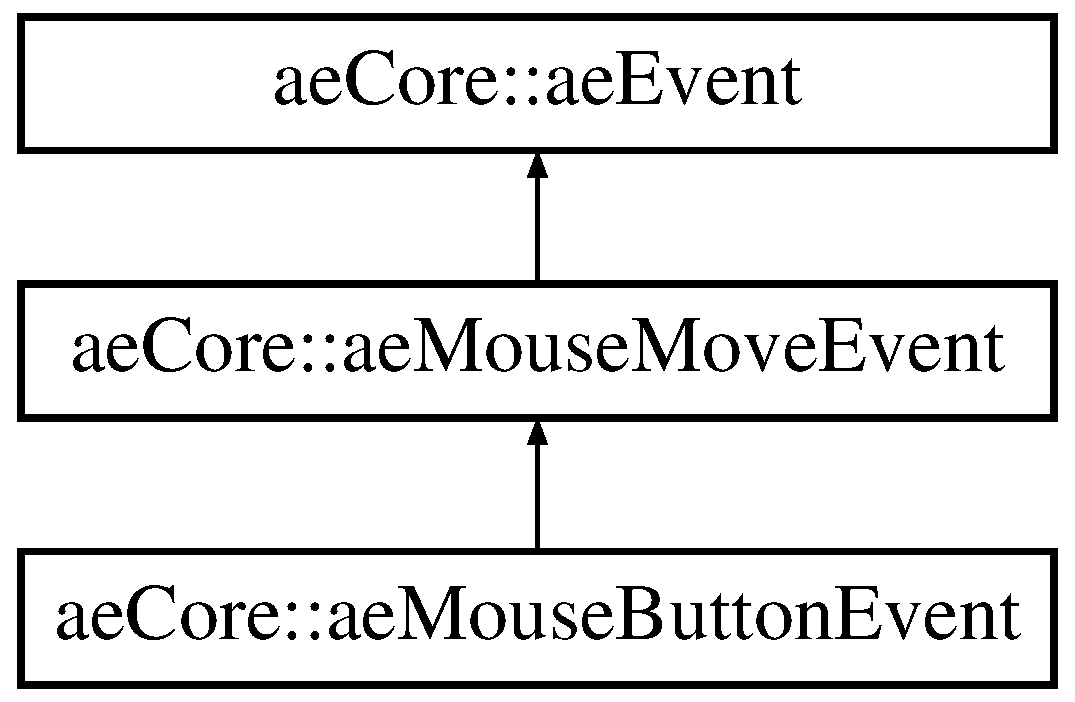
\includegraphics[height=3.000000cm]{structae_core_1_1ae_mouse_button_event}
\end{center}
\end{figure}
\subsection*{Public Attributes}
\begin{DoxyCompactItemize}
\item 
\hyperlink{namespaceae_core_aa13093dc911869e5b24942552898f01f}{uint8} {\bfseries Button}\hypertarget{structae_core_1_1ae_mouse_button_event_a7174e0c8635d450c50e8271f9fcd5817}{}\label{structae_core_1_1ae_mouse_button_event_a7174e0c8635d450c50e8271f9fcd5817}

\item 
\hyperlink{namespaceae_core_aa13093dc911869e5b24942552898f01f}{uint8} {\bfseries State}\hypertarget{structae_core_1_1ae_mouse_button_event_a9c0ab87529ea05ece571c2bf9fe7e05b}{}\label{structae_core_1_1ae_mouse_button_event_a9c0ab87529ea05ece571c2bf9fe7e05b}

\end{DoxyCompactItemize}


\subsection{Detailed Description}
A mouse button event. 

The documentation for this struct was generated from the following file\+:\begin{DoxyCompactItemize}
\item 
C\+:/\+Users/\+Alvaro Estrada/\+Documents/\+Visual Studio 2015/\+Projects/\+R\+T\+S\+\_\+\+A\+E/ae\+Core/\+Event\+System/Events\+System.\+h\end{DoxyCompactItemize}

\hypertarget{structae_core_1_1ae_mouse_move_event}{}\section{ae\+Core\+:\+:ae\+Mouse\+Move\+Event Struct Reference}
\label{structae_core_1_1ae_mouse_move_event}\index{ae\+Core\+::ae\+Mouse\+Move\+Event@{ae\+Core\+::ae\+Mouse\+Move\+Event}}


A .  




{\ttfamily \#include $<$Events\+System.\+h$>$}

Inheritance diagram for ae\+Core\+:\+:ae\+Mouse\+Move\+Event\+:\begin{figure}[H]
\begin{center}
\leavevmode
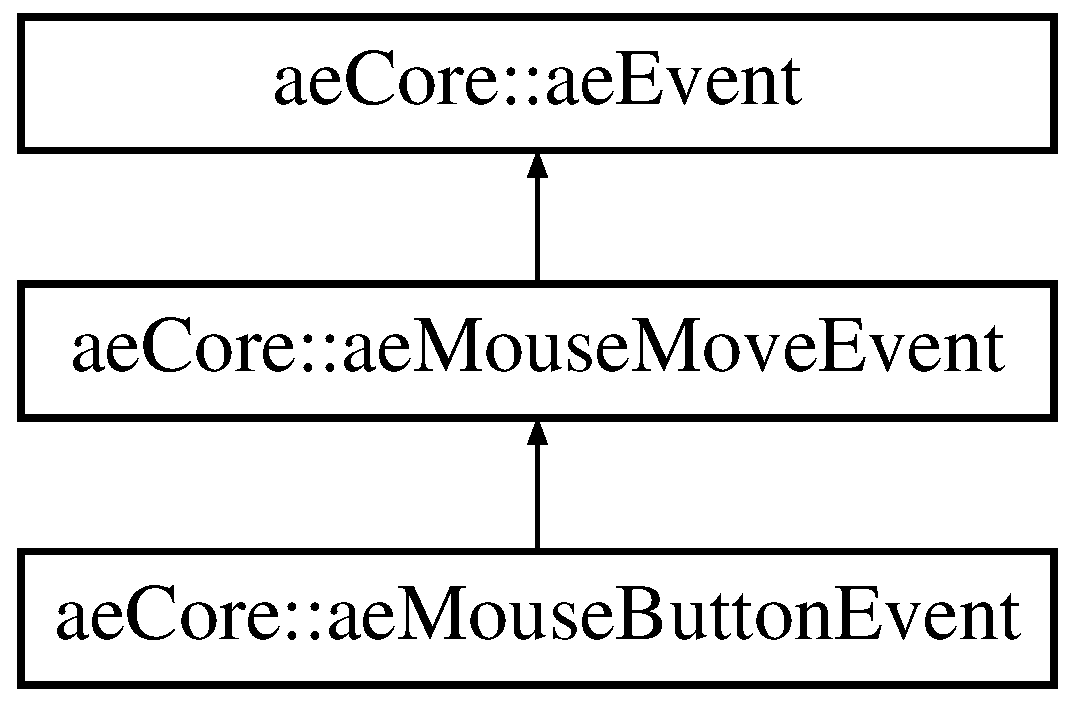
\includegraphics[height=3.000000cm]{structae_core_1_1ae_mouse_move_event}
\end{center}
\end{figure}
\subsection*{Public Attributes}
\begin{DoxyCompactItemize}
\item 
\hyperlink{namespaceae_core_a1f9c426e6389a4ee13ee36ad25ec447d}{uint16} {\bfseries x}\hypertarget{structae_core_1_1ae_mouse_move_event_ac3bd28b095a2cd471a868e561a50d600}{}\label{structae_core_1_1ae_mouse_move_event_ac3bd28b095a2cd471a868e561a50d600}

\item 
\hyperlink{namespaceae_core_a1f9c426e6389a4ee13ee36ad25ec447d}{uint16} {\bfseries y}\hypertarget{structae_core_1_1ae_mouse_move_event_add18c87b983245d75fb661180ff3b5ba}{}\label{structae_core_1_1ae_mouse_move_event_add18c87b983245d75fb661180ff3b5ba}

\end{DoxyCompactItemize}


\subsection{Detailed Description}
A . 

The documentation for this struct was generated from the following file\+:\begin{DoxyCompactItemize}
\item 
C\+:/\+Users/\+Alvaro Estrada/\+Documents/\+Visual Studio 2015/\+Projects/\+R\+T\+S\+\_\+\+A\+E/ae\+Core/\+Event\+System/Events\+System.\+h\end{DoxyCompactItemize}

\hypertarget{classae_path_finder}{}\section{ae\+Path\+Finder Class Reference}
\label{classae_path_finder}\index{ae\+Path\+Finder@{ae\+Path\+Finder}}


A path finder algorithm for the ae\+Tile\+Map Class.  




{\ttfamily \#include $<$Path\+Finder.\+h$>$}

Inheritance diagram for ae\+Path\+Finder\+:\begin{figure}[H]
\begin{center}
\leavevmode
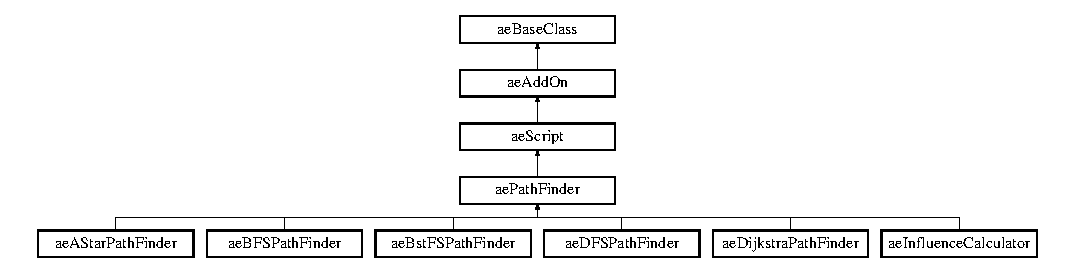
\includegraphics[height=3.240741cm]{classae_path_finder}
\end{center}
\end{figure}
\subsection*{Public Member Functions}
\begin{DoxyCompactItemize}
\item 
{\bfseries ae\+Path\+Finder} (\hyperlink{classae_tiled_map}{ae\+Tiled\+Map} $\ast$p\+Map)\hypertarget{classae_path_finder_a7904f541e7bb5b0ca238bf166ca43625}{}\label{classae_path_finder_a7904f541e7bb5b0ca238bf166ca43625}

\item 
virtual int \hyperlink{classae_path_finder_a3395375f3de8f3f55d7b780ff6815806}{Init} (\hyperlink{classae_base_class}{ae\+Base\+Class} $\ast$p\+Parent)
\begin{DoxyCompactList}\small\item\em Initializes with the given parent pointer. \end{DoxyCompactList}\item 
virtual void \hyperlink{classae_path_finder_a4964df1caa03a0ea9b9c000248bc5ecd}{Reset} ()=0\hypertarget{classae_path_finder_a4964df1caa03a0ea9b9c000248bc5ecd}{}\label{classae_path_finder_a4964df1caa03a0ea9b9c000248bc5ecd}

\begin{DoxyCompactList}\small\item\em Resets this object. \end{DoxyCompactList}\item 
virtual bool \hyperlink{classae_path_finder_a76dad98c8f1c7b3be8688d549fc2fbaf}{Weighted\+Graph\+Supported} ()
\begin{DoxyCompactList}\small\item\em Determines if the pathfinder is weighted graph supported. \end{DoxyCompactList}\item 
virtual bool \hyperlink{classae_path_finder_a07e505593b1af2c3c35854e8d8b21708}{Heuristics\+Supported} ()
\begin{DoxyCompactList}\small\item\em Determines if the pathfinder is heuristics supported. \end{DoxyCompactList}\item 
int \hyperlink{classae_path_finder_a6f6d0af491e9a4ee7fa59999d2bfe24a}{Get\+State} ()
\begin{DoxyCompactList}\small\item\em Gets the state. \end{DoxyCompactList}\item 
void \hyperlink{classae_path_finder_a14af2094678cc4c41726e7fa3aadcc22}{Debug\+Mode} (bool \hyperlink{_base_class_8h_aded8224779c70fab5084220935d672bba46a2a41cc6e552044816a2d04634545d}{State})
\begin{DoxyCompactList}\small\item\em Turns on or off the debug mode. \end{DoxyCompactList}\item 
virtual void \hyperlink{classae_path_finder_a0acb8baba84dacf01734583b258ed89a}{Set\+Start\+Position} (\hyperlink{structae_core_1_1ae_point}{ae\+Point} Start\+Position)
\begin{DoxyCompactList}\small\item\em Sets start position. \end{DoxyCompactList}\item 
void \hyperlink{classae_path_finder_a40cc0daab301f20f1f297d95452ff416}{Set\+End\+Position} (\hyperlink{structae_core_1_1ae_point}{ae\+Point} End\+Position)
\begin{DoxyCompactList}\small\item\em Sets end position. \end{DoxyCompactList}\item 
void \hyperlink{classae_path_finder_ae3087e7f5c1ef96f1c9f0b3674d93983}{Make\+Search} (\hyperlink{structae_core_1_1ae_point}{ae\+Point} Start\+Position, \hyperlink{structae_core_1_1ae_point}{ae\+Point} End\+Position)
\begin{DoxyCompactList}\small\item\em Makes a search. \end{DoxyCompactList}\item 
\hyperlink{structae_core_1_1ae_point}{ae\+Point} \hyperlink{classae_path_finder_a2b20c5c33afbc05c813f60a57be42a39}{Get\+Start\+Position} ()
\begin{DoxyCompactList}\small\item\em Gets start position. \end{DoxyCompactList}\item 
\hyperlink{structae_core_1_1ae_point}{ae\+Point} \hyperlink{classae_path_finder_a5c5719d519644c25f31bd4edd266383a}{Get\+End\+Position} ()
\begin{DoxyCompactList}\small\item\em Gets end position. \end{DoxyCompactList}\item 
uint8 {\bfseries Get\+ID} ()\hypertarget{classae_path_finder_a444cf0bde9683c6df8645df9223e6d26}{}\label{classae_path_finder_a444cf0bde9683c6df8645df9223e6d26}

\end{DoxyCompactItemize}
\subsection*{Protected Member Functions}
\begin{DoxyCompactItemize}
\item 
virtual void \hyperlink{classae_path_finder_a4ccfa19ff344b9f4827dbeab18c4efab}{Visit\+Grid\+Node} (int32 x, int32 y)=0
\begin{DoxyCompactList}\small\item\em Marks a node as visited. \end{DoxyCompactList}\item 
virtual Walk\+State\+ID \hyperlink{classae_path_finder_a49332ee3be744cac1ece9ffd503ca218}{Give\+A\+Step} ()=0
\begin{DoxyCompactList}\small\item\em Give a step. \end{DoxyCompactList}\end{DoxyCompactItemize}
\subsection*{Protected Attributes}
\begin{DoxyCompactItemize}
\item 
ae\+Point {\bfseries m\+\_\+\+Start}\hypertarget{classae_path_finder_a304ea1f079d92518e005a934cfec231a}{}\label{classae_path_finder_a304ea1f079d92518e005a934cfec231a}

\item 
ae\+Point {\bfseries m\+\_\+\+End}\hypertarget{classae_path_finder_af43d9dcda8dd8c7565237871f8ab58da}{}\label{classae_path_finder_af43d9dcda8dd8c7565237871f8ab58da}

\item 
Walk\+State\+ID {\bfseries m\+\_\+\+State}\hypertarget{classae_path_finder_a631071ea16c073ac8fff48524ff8b2a5}{}\label{classae_path_finder_a631071ea16c073ac8fff48524ff8b2a5}

\item 
bool {\bfseries m\+\_\+b\+Debug}\hypertarget{classae_path_finder_a478b1d877cd84d6d0d9454634686c28a}{}\label{classae_path_finder_a478b1d877cd84d6d0d9454634686c28a}

\item 
uint8 {\bfseries m\+\_\+\+ID}\hypertarget{classae_path_finder_a9c4a1b7645a15f6df70b5f9a9e6fc8ef}{}\label{classae_path_finder_a9c4a1b7645a15f6df70b5f9a9e6fc8ef}

\end{DoxyCompactItemize}


\subsection{Detailed Description}
A path finder algorithm for the ae\+Tile\+Map Class. 

\subsection{Member Function Documentation}
\index{ae\+Path\+Finder@{ae\+Path\+Finder}!Debug\+Mode@{Debug\+Mode}}
\index{Debug\+Mode@{Debug\+Mode}!ae\+Path\+Finder@{ae\+Path\+Finder}}
\subsubsection[{\texorpdfstring{Debug\+Mode(bool State)}{DebugMode(bool State)}}]{\setlength{\rightskip}{0pt plus 5cm}void ae\+Path\+Finder\+::\+Debug\+Mode (
\begin{DoxyParamCaption}
\item[{bool}]{State}
\end{DoxyParamCaption}
)}\hypertarget{classae_path_finder_a14af2094678cc4c41726e7fa3aadcc22}{}\label{classae_path_finder_a14af2094678cc4c41726e7fa3aadcc22}


Turns on or off the debug mode. 


\begin{DoxyParams}{Parameters}
{\em State} & true to state. \\
\hline
\end{DoxyParams}
\index{ae\+Path\+Finder@{ae\+Path\+Finder}!Get\+End\+Position@{Get\+End\+Position}}
\index{Get\+End\+Position@{Get\+End\+Position}!ae\+Path\+Finder@{ae\+Path\+Finder}}
\subsubsection[{\texorpdfstring{Get\+End\+Position()}{GetEndPosition()}}]{\setlength{\rightskip}{0pt plus 5cm}{\bf ae\+Point} ae\+Path\+Finder\+::\+Get\+End\+Position (
\begin{DoxyParamCaption}
{}
\end{DoxyParamCaption}
)}\hypertarget{classae_path_finder_a5c5719d519644c25f31bd4edd266383a}{}\label{classae_path_finder_a5c5719d519644c25f31bd4edd266383a}


Gets end position. 

\begin{DoxyReturn}{Returns}
The end position. 
\end{DoxyReturn}
\index{ae\+Path\+Finder@{ae\+Path\+Finder}!Get\+Start\+Position@{Get\+Start\+Position}}
\index{Get\+Start\+Position@{Get\+Start\+Position}!ae\+Path\+Finder@{ae\+Path\+Finder}}
\subsubsection[{\texorpdfstring{Get\+Start\+Position()}{GetStartPosition()}}]{\setlength{\rightskip}{0pt plus 5cm}{\bf ae\+Point} ae\+Path\+Finder\+::\+Get\+Start\+Position (
\begin{DoxyParamCaption}
{}
\end{DoxyParamCaption}
)}\hypertarget{classae_path_finder_a2b20c5c33afbc05c813f60a57be42a39}{}\label{classae_path_finder_a2b20c5c33afbc05c813f60a57be42a39}


Gets start position. 

\begin{DoxyReturn}{Returns}
The start position. 
\end{DoxyReturn}
\index{ae\+Path\+Finder@{ae\+Path\+Finder}!Get\+State@{Get\+State}}
\index{Get\+State@{Get\+State}!ae\+Path\+Finder@{ae\+Path\+Finder}}
\subsubsection[{\texorpdfstring{Get\+State()}{GetState()}}]{\setlength{\rightskip}{0pt plus 5cm}int ae\+Path\+Finder\+::\+Get\+State (
\begin{DoxyParamCaption}
{}
\end{DoxyParamCaption}
)}\hypertarget{classae_path_finder_a6f6d0af491e9a4ee7fa59999d2bfe24a}{}\label{classae_path_finder_a6f6d0af491e9a4ee7fa59999d2bfe24a}


Gets the state. 

\begin{DoxyReturn}{Returns}
The state. 
\end{DoxyReturn}
\index{ae\+Path\+Finder@{ae\+Path\+Finder}!Give\+A\+Step@{Give\+A\+Step}}
\index{Give\+A\+Step@{Give\+A\+Step}!ae\+Path\+Finder@{ae\+Path\+Finder}}
\subsubsection[{\texorpdfstring{Give\+A\+Step()=0}{GiveAStep()=0}}]{\setlength{\rightskip}{0pt plus 5cm}Walk\+State\+ID ae\+Path\+Finder\+::\+Give\+A\+Step (
\begin{DoxyParamCaption}
{}
\end{DoxyParamCaption}
)\hspace{0.3cm}{\ttfamily [protected]}, {\ttfamily [pure virtual]}}\hypertarget{classae_path_finder_a49332ee3be744cac1ece9ffd503ca218}{}\label{classae_path_finder_a49332ee3be744cac1ece9ffd503ca218}


Give a step. 

\begin{DoxyReturn}{Returns}
A Walk\+State\+ID. 
\end{DoxyReturn}


Implemented in \hyperlink{classae_influence_calculator_aff6d5b8b52fb73a4c87a3b311adc6245}{ae\+Influence\+Calculator}, \hyperlink{classae_bst_f_s_path_finder_a172082a7d5f6de9d5163991c076455ca}{ae\+Bst\+F\+S\+Path\+Finder}, \hyperlink{classae_b_f_s_path_finder_a92b13a108bd1151d796dba5a3426704c}{ae\+B\+F\+S\+Path\+Finder}, \hyperlink{classae_a_star_path_finder_a3a23dcf11eccaf75a71179c602ebb1b0}{ae\+A\+Star\+Path\+Finder}, \hyperlink{classae_dijkstra_path_finder_a14ca862aa79790d77d1df8d54f99aa39}{ae\+Dijkstra\+Path\+Finder}, and \hyperlink{classae_d_f_s_path_finder_a752e123b4e24cf7af2f11a3077ace616}{ae\+D\+F\+S\+Path\+Finder}.

\index{ae\+Path\+Finder@{ae\+Path\+Finder}!Heuristics\+Supported@{Heuristics\+Supported}}
\index{Heuristics\+Supported@{Heuristics\+Supported}!ae\+Path\+Finder@{ae\+Path\+Finder}}
\subsubsection[{\texorpdfstring{Heuristics\+Supported()}{HeuristicsSupported()}}]{\setlength{\rightskip}{0pt plus 5cm}bool ae\+Path\+Finder\+::\+Heuristics\+Supported (
\begin{DoxyParamCaption}
{}
\end{DoxyParamCaption}
)\hspace{0.3cm}{\ttfamily [virtual]}}\hypertarget{classae_path_finder_a07e505593b1af2c3c35854e8d8b21708}{}\label{classae_path_finder_a07e505593b1af2c3c35854e8d8b21708}


Determines if the pathfinder is heuristics supported. 

\begin{DoxyReturn}{Returns}
true if it succeeds, false if it fails. 
\end{DoxyReturn}
\index{ae\+Path\+Finder@{ae\+Path\+Finder}!Init@{Init}}
\index{Init@{Init}!ae\+Path\+Finder@{ae\+Path\+Finder}}
\subsubsection[{\texorpdfstring{Init(ae\+Base\+Class $\ast$p\+Parent)}{Init(aeBaseClass *pParent)}}]{\setlength{\rightskip}{0pt plus 5cm}int ae\+Path\+Finder\+::\+Init (
\begin{DoxyParamCaption}
\item[{{\bf ae\+Base\+Class} $\ast$}]{p\+Parent}
\end{DoxyParamCaption}
)\hspace{0.3cm}{\ttfamily [virtual]}}\hypertarget{classae_path_finder_a3395375f3de8f3f55d7b780ff6815806}{}\label{classae_path_finder_a3395375f3de8f3f55d7b780ff6815806}


Initializes with the given parent pointer. 


\begin{DoxyParams}[1]{Parameters}
\mbox{\tt in,out}  & {\em p\+Parent} & If non-\/null, the parent.\\
\hline
\end{DoxyParams}
\begin{DoxyReturn}{Returns}
An int. 
\end{DoxyReturn}


Implements \hyperlink{classae_add_on_a0730c1446e548031f9a4e98435a54675}{ae\+Add\+On}.



Reimplemented in \hyperlink{classae_a_star_path_finder_ad8de2ad34565b3870ab6ed8c7235cd71}{ae\+A\+Star\+Path\+Finder}, \hyperlink{classae_dijkstra_path_finder_a0cc9454fad1387bba68f879afb1f2526}{ae\+Dijkstra\+Path\+Finder}, \hyperlink{classae_bst_f_s_path_finder_a83e0028b1394744dc56b703532a88b40}{ae\+Bst\+F\+S\+Path\+Finder}, \hyperlink{classae_b_f_s_path_finder_a23a16f3e98f5c9fc3a6f56a26a7bf170}{ae\+B\+F\+S\+Path\+Finder}, \hyperlink{classae_influence_calculator_ab2607b3e3750770bb23d7e8c4610a49c}{ae\+Influence\+Calculator}, and \hyperlink{classae_d_f_s_path_finder_a520c7725e3322b43fd7320da622c1b75}{ae\+D\+F\+S\+Path\+Finder}.

\index{ae\+Path\+Finder@{ae\+Path\+Finder}!Make\+Search@{Make\+Search}}
\index{Make\+Search@{Make\+Search}!ae\+Path\+Finder@{ae\+Path\+Finder}}
\subsubsection[{\texorpdfstring{Make\+Search(ae\+Point Start\+Position, ae\+Point End\+Position)}{MakeSearch(aePoint StartPosition, aePoint EndPosition)}}]{\setlength{\rightskip}{0pt plus 5cm}void ae\+Path\+Finder\+::\+Make\+Search (
\begin{DoxyParamCaption}
\item[{{\bf ae\+Point}}]{Start\+Position, }
\item[{{\bf ae\+Point}}]{End\+Position}
\end{DoxyParamCaption}
)}\hypertarget{classae_path_finder_ae3087e7f5c1ef96f1c9f0b3674d93983}{}\label{classae_path_finder_ae3087e7f5c1ef96f1c9f0b3674d93983}


Makes a search. 


\begin{DoxyParams}{Parameters}
{\em Start\+Position} & The start position. \\
\hline
{\em End\+Position} & The end position. \\
\hline
\end{DoxyParams}
\index{ae\+Path\+Finder@{ae\+Path\+Finder}!Set\+End\+Position@{Set\+End\+Position}}
\index{Set\+End\+Position@{Set\+End\+Position}!ae\+Path\+Finder@{ae\+Path\+Finder}}
\subsubsection[{\texorpdfstring{Set\+End\+Position(ae\+Point End\+Position)}{SetEndPosition(aePoint EndPosition)}}]{\setlength{\rightskip}{0pt plus 5cm}void ae\+Path\+Finder\+::\+Set\+End\+Position (
\begin{DoxyParamCaption}
\item[{{\bf ae\+Point}}]{End\+Position}
\end{DoxyParamCaption}
)}\hypertarget{classae_path_finder_a40cc0daab301f20f1f297d95452ff416}{}\label{classae_path_finder_a40cc0daab301f20f1f297d95452ff416}


Sets end position. 


\begin{DoxyParams}{Parameters}
{\em End\+Position} & The end position. \\
\hline
\end{DoxyParams}
\index{ae\+Path\+Finder@{ae\+Path\+Finder}!Set\+Start\+Position@{Set\+Start\+Position}}
\index{Set\+Start\+Position@{Set\+Start\+Position}!ae\+Path\+Finder@{ae\+Path\+Finder}}
\subsubsection[{\texorpdfstring{Set\+Start\+Position(ae\+Point Start\+Position)}{SetStartPosition(aePoint StartPosition)}}]{\setlength{\rightskip}{0pt plus 5cm}void ae\+Path\+Finder\+::\+Set\+Start\+Position (
\begin{DoxyParamCaption}
\item[{{\bf ae\+Point}}]{Start\+Position}
\end{DoxyParamCaption}
)\hspace{0.3cm}{\ttfamily [virtual]}}\hypertarget{classae_path_finder_a0acb8baba84dacf01734583b258ed89a}{}\label{classae_path_finder_a0acb8baba84dacf01734583b258ed89a}


Sets start position. 


\begin{DoxyParams}{Parameters}
{\em Start\+Position} & The start position. \\
\hline
\end{DoxyParams}
\index{ae\+Path\+Finder@{ae\+Path\+Finder}!Visit\+Grid\+Node@{Visit\+Grid\+Node}}
\index{Visit\+Grid\+Node@{Visit\+Grid\+Node}!ae\+Path\+Finder@{ae\+Path\+Finder}}
\subsubsection[{\texorpdfstring{Visit\+Grid\+Node(int32 x, int32 y)=0}{VisitGridNode(int32 x, int32 y)=0}}]{\setlength{\rightskip}{0pt plus 5cm}void ae\+Path\+Finder\+::\+Visit\+Grid\+Node (
\begin{DoxyParamCaption}
\item[{int32}]{x, }
\item[{int32}]{y}
\end{DoxyParamCaption}
)\hspace{0.3cm}{\ttfamily [protected]}, {\ttfamily [pure virtual]}}\hypertarget{classae_path_finder_a4ccfa19ff344b9f4827dbeab18c4efab}{}\label{classae_path_finder_a4ccfa19ff344b9f4827dbeab18c4efab}


Marks a node as visited. 


\begin{DoxyParams}{Parameters}
{\em x} & The x coordinate. \\
\hline
{\em y} & The y coordinate. \\
\hline
\end{DoxyParams}


Implemented in \hyperlink{classae_influence_calculator_a8f31c5a25ca68ef970247f608bb51917}{ae\+Influence\+Calculator}, \hyperlink{classae_a_star_path_finder_a3263c66da32aea8e2f6567754110c63c}{ae\+A\+Star\+Path\+Finder}, \hyperlink{classae_dijkstra_path_finder_a06cbc7f3215eb10e66bffc69cd051dae}{ae\+Dijkstra\+Path\+Finder}, \hyperlink{classae_bst_f_s_path_finder_ae46add3c2ab1986423288bde7f92bcf0}{ae\+Bst\+F\+S\+Path\+Finder}, \hyperlink{classae_b_f_s_path_finder_a92683a0590099c03c5a0527fc7d11ae0}{ae\+B\+F\+S\+Path\+Finder}, and \hyperlink{classae_d_f_s_path_finder_a9a15c735ca42c68cb129641d79579be2}{ae\+D\+F\+S\+Path\+Finder}.

\index{ae\+Path\+Finder@{ae\+Path\+Finder}!Weighted\+Graph\+Supported@{Weighted\+Graph\+Supported}}
\index{Weighted\+Graph\+Supported@{Weighted\+Graph\+Supported}!ae\+Path\+Finder@{ae\+Path\+Finder}}
\subsubsection[{\texorpdfstring{Weighted\+Graph\+Supported()}{WeightedGraphSupported()}}]{\setlength{\rightskip}{0pt plus 5cm}bool ae\+Path\+Finder\+::\+Weighted\+Graph\+Supported (
\begin{DoxyParamCaption}
{}
\end{DoxyParamCaption}
)\hspace{0.3cm}{\ttfamily [virtual]}}\hypertarget{classae_path_finder_a76dad98c8f1c7b3be8688d549fc2fbaf}{}\label{classae_path_finder_a76dad98c8f1c7b3be8688d549fc2fbaf}


Determines if the pathfinder is weighted graph supported. 

\begin{DoxyReturn}{Returns}
true if it succeeds, false if it fails. 
\end{DoxyReturn}


The documentation for this class was generated from the following files\+:\begin{DoxyCompactItemize}
\item 
C\+:/\+Users/\+Alvaro Estrada/\+Documents/\+Visual Studio 2015/\+Projects/\+R\+T\+S\+\_\+\+A\+E/\+R\+T\+S\+\_\+\+A\+E/\+Game/\hyperlink{_path_finder_8h}{Path\+Finder.\+h}\item 
C\+:/\+Users/\+Alvaro Estrada/\+Documents/\+Visual Studio 2015/\+Projects/\+R\+T\+S\+\_\+\+A\+E/\+R\+T\+S\+\_\+\+A\+E/\+Game/\hyperlink{_path_finder_8cpp}{Path\+Finder.\+cpp}\end{DoxyCompactItemize}

\hypertarget{structae_core_1_1ae_point}{}\section{ae\+Core\+:\+:ae\+Point Struct Reference}
\label{structae_core_1_1ae_point}\index{ae\+Core\+::ae\+Point@{ae\+Core\+::ae\+Point}}


It\textquotesingle{}s a 2 elements structure, it has an union between integer values x and w, and also y and h; it\textquotesingle{}s for easy access.  




{\ttfamily \#include $<$Basic\+Classes.\+h$>$}

\subsection*{Public Member Functions}
\begin{DoxyCompactItemize}
\item 
{\bfseries ae\+Point} (const \hyperlink{structae_core_1_1ae_point}{ae\+Point} \&Other)\hypertarget{structae_core_1_1ae_point_ac80be6903e68ecc4c168d98987c2d989}{}\label{structae_core_1_1ae_point_ac80be6903e68ecc4c168d98987c2d989}

\item 
{\bfseries ae\+Point} (int X, int Y)\hypertarget{structae_core_1_1ae_point_aebb984a4502e4d670dadc214e3541488}{}\label{structae_core_1_1ae_point_aebb984a4502e4d670dadc214e3541488}

\end{DoxyCompactItemize}
\subsection*{Public Attributes}
\begin{DoxyCompactItemize}
\item 
\begin{tabbing}
xx\=xx\=xx\=xx\=xx\=xx\=xx\=xx\=xx\=\kill
union \{\\
\>struct \{\\
\>\>int {\bfseries x}\\
\>\>int {\bfseries y}\\
\>\} \hypertarget{unionae_core_1_1ae_point_1_1_0D0_ab375d2cd78e5102c8b9ab65f06a8b4c9}{}\label{unionae_core_1_1ae_point_1_1_0D0_ab375d2cd78e5102c8b9ab65f06a8b4c9}
\\
\>struct \{\\
\>\>int {\bfseries w}\\
\>\>int {\bfseries h}\\
\>\} \hypertarget{unionae_core_1_1ae_point_1_1_0D0_a3282ec6603c4c243656021cfa7ddb914}{}\label{unionae_core_1_1ae_point_1_1_0D0_a3282ec6603c4c243656021cfa7ddb914}
\\
\}; \hypertarget{structae_core_1_1ae_point_aa9c2b049ab3cf5115115f411c1486296}{}\label{structae_core_1_1ae_point_aa9c2b049ab3cf5115115f411c1486296}
\\

\end{tabbing}\end{DoxyCompactItemize}


\subsection{Detailed Description}
It\textquotesingle{}s a 2 elements structure, it has an union between integer values x and w, and also y and h; it\textquotesingle{}s for easy access. 

The documentation for this struct was generated from the following file\+:\begin{DoxyCompactItemize}
\item 
C\+:/\+Users/\+Alvaro Estrada/\+Documents/\+Visual Studio 2015/\+Projects/\+R\+T\+S\+\_\+\+A\+E/ae\+Core/Basic\+Classes.\+h\end{DoxyCompactItemize}

\hypertarget{classae_presets}{}\section{ae\+Presets Class Reference}
\label{classae_presets}\index{ae\+Presets@{ae\+Presets}}


A presets.  




{\ttfamily \#include $<$Presets.\+h$>$}

Inheritance diagram for ae\+Presets\+:\begin{figure}[H]
\begin{center}
\leavevmode
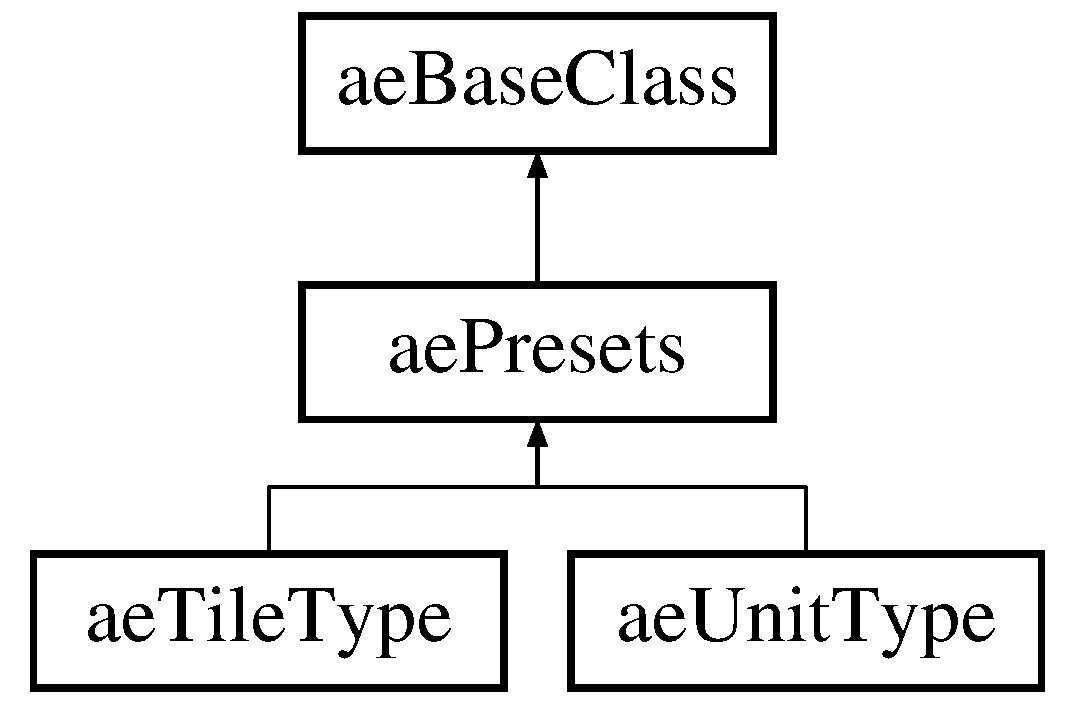
\includegraphics[height=3.000000cm]{classae_presets}
\end{center}
\end{figure}
\subsection*{Public Member Functions}
\begin{DoxyCompactItemize}
\item 
virtual void \hyperlink{classae_presets_ab3b99e89c0edc19b9dfcaa4f9dda4cac}{Destroy} ()\hypertarget{classae_presets_ab3b99e89c0edc19b9dfcaa4f9dda4cac}{}\label{classae_presets_ab3b99e89c0edc19b9dfcaa4f9dda4cac}

\begin{DoxyCompactList}\small\item\em Destroys this object. \end{DoxyCompactList}\item 
int {\bfseries Get\+Preset\+ID} ()\hypertarget{classae_presets_a2b2922ffc74513c8819ba5ddd161b449}{}\label{classae_presets_a2b2922ffc74513c8819ba5ddd161b449}

\end{DoxyCompactItemize}
\subsection*{Protected Attributes}
\begin{DoxyCompactItemize}
\item 
int {\bfseries m\+\_\+n\+Preset\+ID}\hypertarget{classae_presets_aff82b5232f037a495d85fe0decbbc61e}{}\label{classae_presets_aff82b5232f037a495d85fe0decbbc61e}

\end{DoxyCompactItemize}


\subsection{Detailed Description}
A presets. 

The documentation for this class was generated from the following files\+:\begin{DoxyCompactItemize}
\item 
C\+:/\+Users/\+Alvaro Estrada/\+Documents/\+Visual Studio 2015/\+Projects/\+R\+T\+S\+\_\+\+A\+E/\+R\+T\+S\+\_\+\+A\+E/\+Game/\hyperlink{_presets_8h}{Presets.\+h}\item 
C\+:/\+Users/\+Alvaro Estrada/\+Documents/\+Visual Studio 2015/\+Projects/\+R\+T\+S\+\_\+\+A\+E/\+R\+T\+S\+\_\+\+A\+E/\+Game/Presets.\+cpp\end{DoxyCompactItemize}

\hypertarget{structae_core_1_1ae_quit_event}{}\section{ae\+Core\+:\+:ae\+Quit\+Event Struct Reference}
\label{structae_core_1_1ae_quit_event}\index{ae\+Core\+::ae\+Quit\+Event@{ae\+Core\+::ae\+Quit\+Event}}


A quit event.  




{\ttfamily \#include $<$Events\+System.\+h$>$}

Inheritance diagram for ae\+Core\+:\+:ae\+Quit\+Event\+:\begin{figure}[H]
\begin{center}
\leavevmode
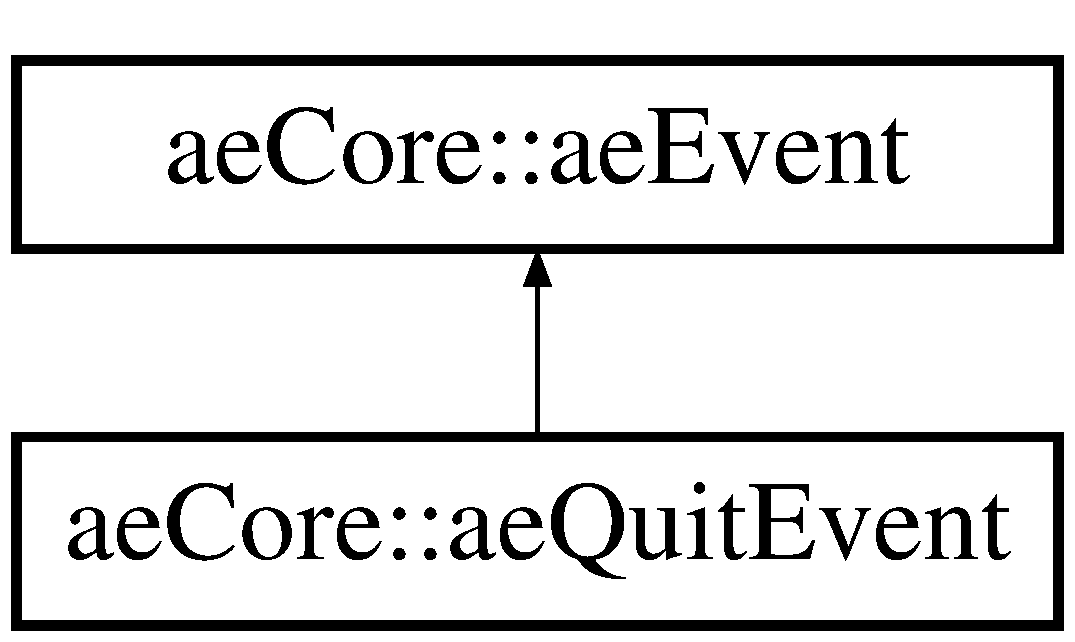
\includegraphics[height=2.000000cm]{structae_core_1_1ae_quit_event}
\end{center}
\end{figure}
\subsection*{Additional Inherited Members}


\subsection{Detailed Description}
A quit event. 

The documentation for this struct was generated from the following file\+:\begin{DoxyCompactItemize}
\item 
C\+:/\+Users/\+Alvaro Estrada/\+Documents/\+Visual Studio 2015/\+Projects/\+R\+T\+S\+\_\+\+A\+E/ae\+Core/\+Event\+System/Events\+System.\+h\end{DoxyCompactItemize}

\hypertarget{structae_core_1_1ae_rect}{}\section{ae\+Core\+:\+:ae\+Rect Struct Reference}
\label{structae_core_1_1ae_rect}\index{ae\+Core\+::ae\+Rect@{ae\+Core\+::ae\+Rect}}


A rectangle.  




{\ttfamily \#include $<$Basic\+Classes.\+h$>$}

\subsection*{Public Member Functions}
\begin{DoxyCompactItemize}
\item 
{\bfseries ae\+Rect} (const \hyperlink{structae_core_1_1ae_rect}{ae\+Rect} \&Other)\hypertarget{structae_core_1_1ae_rect_a8fe58b407f8632a98c1d39c711cc2962}{}\label{structae_core_1_1ae_rect_a8fe58b407f8632a98c1d39c711cc2962}

\item 
{\bfseries ae\+Rect} (int X, int Y, int W, int H)\hypertarget{structae_core_1_1ae_rect_a060a4d7ff58761509903faef941d65bf}{}\label{structae_core_1_1ae_rect_a060a4d7ff58761509903faef941d65bf}

\item 
bool {\bfseries Hit\+Test} (int X, int Y)\hypertarget{structae_core_1_1ae_rect_a75326d8a1549f011f5afaf75db74dc3f}{}\label{structae_core_1_1ae_rect_a75326d8a1549f011f5afaf75db74dc3f}

\end{DoxyCompactItemize}
\subsection*{Public Attributes}
\begin{DoxyCompactItemize}
\item 
int {\bfseries x}\hypertarget{structae_core_1_1ae_rect_a80094e4251c2bdf1d07fb71afc2b9a26}{}\label{structae_core_1_1ae_rect_a80094e4251c2bdf1d07fb71afc2b9a26}

\item 
int {\bfseries y}\hypertarget{structae_core_1_1ae_rect_a67520f1b61e0a7195cafc465f4b8fd41}{}\label{structae_core_1_1ae_rect_a67520f1b61e0a7195cafc465f4b8fd41}

\item 
int {\bfseries w}\hypertarget{structae_core_1_1ae_rect_ae7f80fe08b22f20e35fe1a3a983da7d8}{}\label{structae_core_1_1ae_rect_ae7f80fe08b22f20e35fe1a3a983da7d8}

\item 
int {\bfseries h}\hypertarget{structae_core_1_1ae_rect_ab96e550c3f109e0decf391c52af5015a}{}\label{structae_core_1_1ae_rect_ab96e550c3f109e0decf391c52af5015a}

\end{DoxyCompactItemize}


\subsection{Detailed Description}
A rectangle. 

The documentation for this struct was generated from the following file\+:\begin{DoxyCompactItemize}
\item 
C\+:/\+Users/\+Alvaro Estrada/\+Documents/\+Visual Studio 2015/\+Projects/\+R\+T\+S\+\_\+\+A\+E/ae\+Core/Basic\+Classes.\+h\end{DoxyCompactItemize}

\hypertarget{classae_core_1_1ae_renderer}{}\section{ae\+Core\+:\+:ae\+Renderer Class Reference}
\label{classae_core_1_1ae_renderer}\index{ae\+Core\+::ae\+Renderer@{ae\+Core\+::ae\+Renderer}}


Stores the window renderer so it can be passed along.  




{\ttfamily \#include $<$Renderer.\+h$>$}

\subsection*{Public Member Functions}
\begin{DoxyCompactItemize}
\item 
\hyperlink{classae_core_1_1ae_renderer_aa98c12f7aeba64e6cd32856ce35b26f4}{ae\+Renderer} ()\hypertarget{classae_core_1_1ae_renderer_aa98c12f7aeba64e6cd32856ce35b26f4}{}\label{classae_core_1_1ae_renderer_aa98c12f7aeba64e6cd32856ce35b26f4}

\begin{DoxyCompactList}\small\item\em Default constructor. \end{DoxyCompactList}\item 
\hyperlink{classae_core_1_1ae_renderer_ac336fe39ee36736b5cfbf47c665a5ad2}{$\sim$ae\+Renderer} ()\hypertarget{classae_core_1_1ae_renderer_ac336fe39ee36736b5cfbf47c665a5ad2}{}\label{classae_core_1_1ae_renderer_ac336fe39ee36736b5cfbf47c665a5ad2}

\begin{DoxyCompactList}\small\item\em Destructor. \end{DoxyCompactList}\item 
void \hyperlink{classae_core_1_1ae_renderer_ad274612bff58ca4707d7e573e48bc0cd}{Clear} ()\hypertarget{classae_core_1_1ae_renderer_ad274612bff58ca4707d7e573e48bc0cd}{}\label{classae_core_1_1ae_renderer_ad274612bff58ca4707d7e573e48bc0cd}

\begin{DoxyCompactList}\small\item\em Clears this object to its blank/initial state. \end{DoxyCompactList}\item 
void \hyperlink{classae_core_1_1ae_renderer_afbc2091d48c14b36f25a2f42b1ff5b04}{Destroy} ()\hypertarget{classae_core_1_1ae_renderer_afbc2091d48c14b36f25a2f42b1ff5b04}{}\label{classae_core_1_1ae_renderer_afbc2091d48c14b36f25a2f42b1ff5b04}

\begin{DoxyCompactList}\small\item\em Destroys this object. \end{DoxyCompactList}\item 
\hyperlink{structae_core_1_1ae_r_g_b_quad}{ae\+R\+G\+B\+Quad} \hyperlink{classae_core_1_1ae_renderer_a3463e48a8794b6ba83ecba3c2d8d3424}{Set\+Render\+Draw\+Color} (\hyperlink{structae_core_1_1ae_r_g_b_quad}{ae\+R\+G\+B\+Quad} Color)
\begin{DoxyCompactList}\small\item\em Sets render draw color. \end{DoxyCompactList}\item 
void \hyperlink{classae_core_1_1ae_renderer_a763bb052c5cea701ec12ab77a164ea5d}{Draw\+Line} (\hyperlink{structae_core_1_1ae_point}{ae\+Point} Start, \hyperlink{structae_core_1_1ae_point}{ae\+Point} End)
\begin{DoxyCompactList}\small\item\em Draw line. \end{DoxyCompactList}\item 
void \hyperlink{classae_core_1_1ae_renderer_ac821b51f9396c9a279dc1bcdf7744560}{Draw\+Rect} (\hyperlink{structae_core_1_1ae_rect}{ae\+Rect} Rectangle)
\begin{DoxyCompactList}\small\item\em Draw rectangle. \end{DoxyCompactList}\item 
void \hyperlink{classae_core_1_1ae_renderer_aa30f051d2ee663a9efc401fc62dcc8a9}{Draw\+Point} (\hyperlink{structae_core_1_1ae_point}{ae\+Point} Point)
\begin{DoxyCompactList}\small\item\em Draw point. \end{DoxyCompactList}\item 
void \hyperlink{classae_core_1_1ae_renderer_a5a069b5046deab1ad7cb87aa1fdb891b}{Render\+Target} (\hyperlink{classae_core_1_1ae_sprite}{ae\+Sprite} $\ast$Target)
\begin{DoxyCompactList}\small\item\em Renders the target described by Target. \end{DoxyCompactList}\end{DoxyCompactItemize}
\subsection*{Friends}
\begin{DoxyCompactItemize}
\item 
class {\bfseries ae\+Sprite}\hypertarget{classae_core_1_1ae_renderer_a450e94d8bab3fa5d26d3663ba55b8ba3}{}\label{classae_core_1_1ae_renderer_a450e94d8bab3fa5d26d3663ba55b8ba3}

\item 
class {\bfseries ae\+App\+Window}\hypertarget{classae_core_1_1ae_renderer_a663f64030555362890326e0b793c8839}{}\label{classae_core_1_1ae_renderer_a663f64030555362890326e0b793c8839}

\end{DoxyCompactItemize}


\subsection{Detailed Description}
Stores the window renderer so it can be passed along. 

\subsection{Member Function Documentation}
\index{ae\+Core\+::ae\+Renderer@{ae\+Core\+::ae\+Renderer}!Draw\+Line@{Draw\+Line}}
\index{Draw\+Line@{Draw\+Line}!ae\+Core\+::ae\+Renderer@{ae\+Core\+::ae\+Renderer}}
\subsubsection[{\texorpdfstring{Draw\+Line(ae\+Point Start, ae\+Point End)}{DrawLine(aePoint Start, aePoint End)}}]{\setlength{\rightskip}{0pt plus 5cm}void ae\+Core\+::ae\+Renderer\+::\+Draw\+Line (
\begin{DoxyParamCaption}
\item[{{\bf ae\+Point}}]{Start, }
\item[{{\bf ae\+Point}}]{End}
\end{DoxyParamCaption}
)}\hypertarget{classae_core_1_1ae_renderer_a763bb052c5cea701ec12ab77a164ea5d}{}\label{classae_core_1_1ae_renderer_a763bb052c5cea701ec12ab77a164ea5d}


Draw line. 


\begin{DoxyParams}{Parameters}
{\em Start} & The start. \\
\hline
{\em End} & The end. \\
\hline
\end{DoxyParams}
\index{ae\+Core\+::ae\+Renderer@{ae\+Core\+::ae\+Renderer}!Draw\+Point@{Draw\+Point}}
\index{Draw\+Point@{Draw\+Point}!ae\+Core\+::ae\+Renderer@{ae\+Core\+::ae\+Renderer}}
\subsubsection[{\texorpdfstring{Draw\+Point(ae\+Point Point)}{DrawPoint(aePoint Point)}}]{\setlength{\rightskip}{0pt plus 5cm}void ae\+Core\+::ae\+Renderer\+::\+Draw\+Point (
\begin{DoxyParamCaption}
\item[{{\bf ae\+Point}}]{Point}
\end{DoxyParamCaption}
)}\hypertarget{classae_core_1_1ae_renderer_aa30f051d2ee663a9efc401fc62dcc8a9}{}\label{classae_core_1_1ae_renderer_aa30f051d2ee663a9efc401fc62dcc8a9}


Draw point. 


\begin{DoxyParams}{Parameters}
{\em Point} & The point. \\
\hline
\end{DoxyParams}
\index{ae\+Core\+::ae\+Renderer@{ae\+Core\+::ae\+Renderer}!Draw\+Rect@{Draw\+Rect}}
\index{Draw\+Rect@{Draw\+Rect}!ae\+Core\+::ae\+Renderer@{ae\+Core\+::ae\+Renderer}}
\subsubsection[{\texorpdfstring{Draw\+Rect(ae\+Rect Rectangle)}{DrawRect(aeRect Rectangle)}}]{\setlength{\rightskip}{0pt plus 5cm}void ae\+Core\+::ae\+Renderer\+::\+Draw\+Rect (
\begin{DoxyParamCaption}
\item[{{\bf ae\+Rect}}]{Rectangle}
\end{DoxyParamCaption}
)}\hypertarget{classae_core_1_1ae_renderer_ac821b51f9396c9a279dc1bcdf7744560}{}\label{classae_core_1_1ae_renderer_ac821b51f9396c9a279dc1bcdf7744560}


Draw rectangle. 


\begin{DoxyParams}{Parameters}
{\em Rectangle} & The Rectangle. \\
\hline
\end{DoxyParams}
\index{ae\+Core\+::ae\+Renderer@{ae\+Core\+::ae\+Renderer}!Render\+Target@{Render\+Target}}
\index{Render\+Target@{Render\+Target}!ae\+Core\+::ae\+Renderer@{ae\+Core\+::ae\+Renderer}}
\subsubsection[{\texorpdfstring{Render\+Target(ae\+Sprite $\ast$\+Target)}{RenderTarget(aeSprite *Target)}}]{\setlength{\rightskip}{0pt plus 5cm}void ae\+Core\+::ae\+Renderer\+::\+Render\+Target (
\begin{DoxyParamCaption}
\item[{{\bf ae\+Sprite} $\ast$}]{Target}
\end{DoxyParamCaption}
)}\hypertarget{classae_core_1_1ae_renderer_a5a069b5046deab1ad7cb87aa1fdb891b}{}\label{classae_core_1_1ae_renderer_a5a069b5046deab1ad7cb87aa1fdb891b}


Renders the target described by Target. 


\begin{DoxyParams}[1]{Parameters}
\mbox{\tt in,out}  & {\em Target} & If non-\/null, target for the. \\
\hline
\end{DoxyParams}
\index{ae\+Core\+::ae\+Renderer@{ae\+Core\+::ae\+Renderer}!Set\+Render\+Draw\+Color@{Set\+Render\+Draw\+Color}}
\index{Set\+Render\+Draw\+Color@{Set\+Render\+Draw\+Color}!ae\+Core\+::ae\+Renderer@{ae\+Core\+::ae\+Renderer}}
\subsubsection[{\texorpdfstring{Set\+Render\+Draw\+Color(ae\+R\+G\+B\+Quad Color)}{SetRenderDrawColor(aeRGBQuad Color)}}]{\setlength{\rightskip}{0pt plus 5cm}{\bf ae\+R\+G\+B\+Quad} ae\+Core\+::ae\+Renderer\+::\+Set\+Render\+Draw\+Color (
\begin{DoxyParamCaption}
\item[{{\bf ae\+R\+G\+B\+Quad}}]{Color}
\end{DoxyParamCaption}
)}\hypertarget{classae_core_1_1ae_renderer_a3463e48a8794b6ba83ecba3c2d8d3424}{}\label{classae_core_1_1ae_renderer_a3463e48a8794b6ba83ecba3c2d8d3424}


Sets render draw color. 


\begin{DoxyParams}{Parameters}
{\em Color} & The color.\\
\hline
\end{DoxyParams}
\begin{DoxyReturn}{Returns}
An \hyperlink{structae_core_1_1ae_r_g_b_quad}{ae\+R\+G\+B\+Quad}. 
\end{DoxyReturn}


The documentation for this class was generated from the following files\+:\begin{DoxyCompactItemize}
\item 
C\+:/\+Users/\+Alvaro Estrada/\+Documents/\+Visual Studio 2015/\+Projects/\+R\+T\+S\+\_\+\+A\+E/ae\+Core/\+Graphics/\hyperlink{_renderer_8h}{Renderer.\+h}\item 
C\+:/\+Users/\+Alvaro Estrada/\+Documents/\+Visual Studio 2015/\+Projects/\+R\+T\+S\+\_\+\+A\+E/ae\+Core/\+Graphics/Renderer.\+cpp\end{DoxyCompactItemize}

\hypertarget{structae_core_1_1ae_resize_event}{}\section{ae\+Core\+:\+:ae\+Resize\+Event Struct Reference}
\label{structae_core_1_1ae_resize_event}\index{ae\+Core\+::ae\+Resize\+Event@{ae\+Core\+::ae\+Resize\+Event}}


A resize event.  




{\ttfamily \#include $<$Events\+System.\+h$>$}

Inheritance diagram for ae\+Core\+:\+:ae\+Resize\+Event\+:\begin{figure}[H]
\begin{center}
\leavevmode
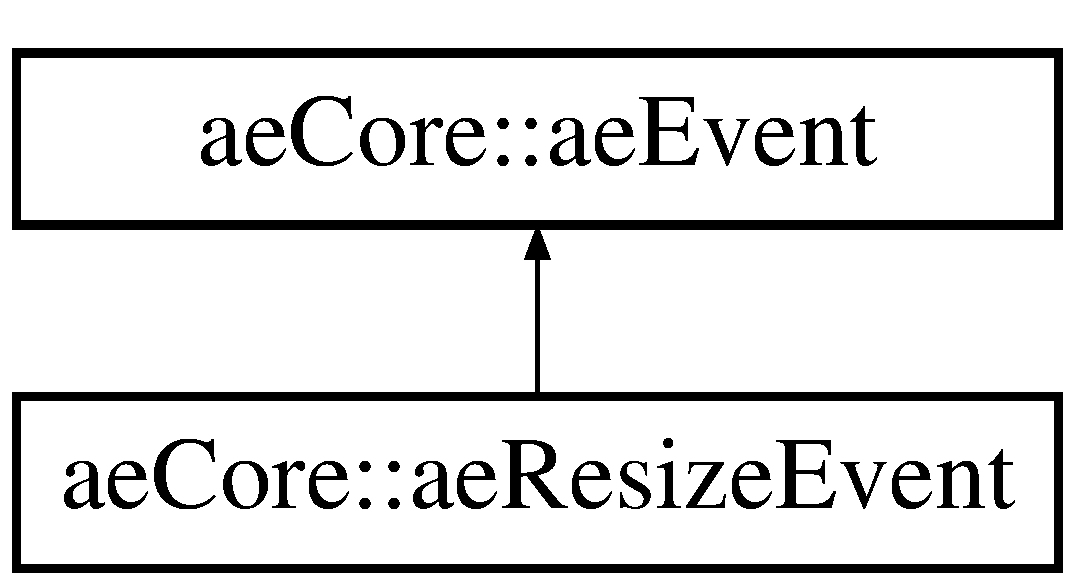
\includegraphics[height=2.000000cm]{structae_core_1_1ae_resize_event}
\end{center}
\end{figure}
\subsection*{Public Attributes}
\begin{DoxyCompactItemize}
\item 
\hyperlink{namespaceae_core_a1f9c426e6389a4ee13ee36ad25ec447d}{uint16} {\bfseries w}\hypertarget{structae_core_1_1ae_resize_event_ac8c75f55c1705aa5fcd015831d924d39}{}\label{structae_core_1_1ae_resize_event_ac8c75f55c1705aa5fcd015831d924d39}

\item 
\hyperlink{namespaceae_core_a1f9c426e6389a4ee13ee36ad25ec447d}{uint16} {\bfseries h}\hypertarget{structae_core_1_1ae_resize_event_a492e181f49f7a7b13f40ebc14677ed0d}{}\label{structae_core_1_1ae_resize_event_a492e181f49f7a7b13f40ebc14677ed0d}

\end{DoxyCompactItemize}


\subsection{Detailed Description}
A resize event. 

The documentation for this struct was generated from the following file\+:\begin{DoxyCompactItemize}
\item 
C\+:/\+Users/\+Alvaro Estrada/\+Documents/\+Visual Studio 2015/\+Projects/\+R\+T\+S\+\_\+\+A\+E/ae\+Core/\+Event\+System/Events\+System.\+h\end{DoxyCompactItemize}

\hypertarget{structae_core_1_1ae_r_g_b}{}\section{ae\+Core\+:\+:ae\+R\+GB Struct Reference}
\label{structae_core_1_1ae_r_g_b}\index{ae\+Core\+::ae\+R\+GB@{ae\+Core\+::ae\+R\+GB}}


Is a color structure with R\+GB capacity.  




{\ttfamily \#include $<$Basic\+Classes.\+h$>$}

\subsection*{Public Member Functions}
\begin{DoxyCompactItemize}
\item 
{\bfseries ae\+R\+GB} (const \hyperlink{structae_core_1_1ae_r_g_b}{ae\+R\+GB} \&Other)\hypertarget{structae_core_1_1ae_r_g_b_acdac34cbf2d4d9fd1ef87580f9f570ee}{}\label{structae_core_1_1ae_r_g_b_acdac34cbf2d4d9fd1ef87580f9f570ee}

\item 
{\bfseries ae\+R\+GB} (\hyperlink{namespaceae_core_aa13093dc911869e5b24942552898f01f}{uint8} R, \hyperlink{namespaceae_core_aa13093dc911869e5b24942552898f01f}{uint8} G, \hyperlink{namespaceae_core_aa13093dc911869e5b24942552898f01f}{uint8} B)\hypertarget{structae_core_1_1ae_r_g_b_a0e17a9e0089139d9d41ac190effeb7d0}{}\label{structae_core_1_1ae_r_g_b_a0e17a9e0089139d9d41ac190effeb7d0}

\item 
{\bfseries ae\+R\+GB} (unsigned \+\_\+\+\_\+int32 C\+O\+L\+OR)\hypertarget{structae_core_1_1ae_r_g_b_aaece8ab7ce759ea24bf945faf4d53665}{}\label{structae_core_1_1ae_r_g_b_aaece8ab7ce759ea24bf945faf4d53665}

\end{DoxyCompactItemize}
\subsection*{Public Attributes}
\begin{DoxyCompactItemize}
\item 
\begin{tabbing}
xx\=xx\=xx\=xx\=xx\=xx\=xx\=xx\=xx\=\kill
union \{\\
\>struct \{\\
\>\>unsigned \_\_int8 {\bfseries r}\\
\>\>unsigned \_\_int8 {\bfseries g}\\
\>\>unsigned \_\_int8 {\bfseries b}\\
\>\} \hypertarget{unionae_core_1_1ae_r_g_b_1_1_0D6_a5f77018757a15205d00cc26e2c87aa04}{}\label{unionae_core_1_1ae_r_g_b_1_1_0D6_a5f77018757a15205d00cc26e2c87aa04}
\\
\>unsigned \_\_int32 {\bfseries Color}\\
\}; \hypertarget{structae_core_1_1ae_r_g_b_a6a903e2f0497e3e60ff936493edc2fc7}{}\label{structae_core_1_1ae_r_g_b_a6a903e2f0497e3e60ff936493edc2fc7}
\\

\end{tabbing}\end{DoxyCompactItemize}


\subsection{Detailed Description}
Is a color structure with R\+GB capacity. 

The documentation for this struct was generated from the following file\+:\begin{DoxyCompactItemize}
\item 
C\+:/\+Users/\+Alvaro Estrada/\+Documents/\+Visual Studio 2015/\+Projects/\+R\+T\+S\+\_\+\+A\+E/ae\+Core/Basic\+Classes.\+h\end{DoxyCompactItemize}

\hypertarget{structae_core_1_1ae_r_g_b_quad}{}\section{ae\+Core\+:\+:ae\+R\+G\+B\+Quad Struct Reference}
\label{structae_core_1_1ae_r_g_b_quad}\index{ae\+Core\+::ae\+R\+G\+B\+Quad@{ae\+Core\+::ae\+R\+G\+B\+Quad}}


Is a color structure with R\+G\+BA capacity.  




{\ttfamily \#include $<$Basic\+Classes.\+h$>$}

\subsection*{Public Member Functions}
\begin{DoxyCompactItemize}
\item 
{\bfseries ae\+R\+G\+B\+Quad} (const \hyperlink{structae_core_1_1ae_r_g_b_quad}{ae\+R\+G\+B\+Quad} \&Other)\hypertarget{structae_core_1_1ae_r_g_b_quad_a35ee8c4e94a64f2ff611ab9cd4e099ee}{}\label{structae_core_1_1ae_r_g_b_quad_a35ee8c4e94a64f2ff611ab9cd4e099ee}

\item 
{\bfseries ae\+R\+G\+B\+Quad} (unsigned char R, unsigned char G, unsigned char B, unsigned char A)\hypertarget{structae_core_1_1ae_r_g_b_quad_a439c01503811646a2d0f5a2d543cf21b}{}\label{structae_core_1_1ae_r_g_b_quad_a439c01503811646a2d0f5a2d543cf21b}

\item 
{\bfseries ae\+R\+G\+B\+Quad} (unsigned \+\_\+\+\_\+int32 C\+O\+L\+OR)\hypertarget{structae_core_1_1ae_r_g_b_quad_af2a4bdd8be5268f72e93d742202136ca}{}\label{structae_core_1_1ae_r_g_b_quad_af2a4bdd8be5268f72e93d742202136ca}

\end{DoxyCompactItemize}
\subsection*{Public Attributes}
\begin{DoxyCompactItemize}
\item 
\begin{tabbing}
xx\=xx\=xx\=xx\=xx\=xx\=xx\=xx\=xx\=\kill
union \{\\
\>struct \{\\
\>\>unsigned \_\_int8 {\bfseries r}\\
\>\>unsigned \_\_int8 {\bfseries g}\\
\>\>unsigned \_\_int8 {\bfseries b}\\
\>\>unsigned \_\_int8 {\bfseries a}\\
\>\} \hypertarget{unionae_core_1_1ae_r_g_b_quad_1_1_0D10_a9102714f11403077da0250f6c893baec}{}\label{unionae_core_1_1ae_r_g_b_quad_1_1_0D10_a9102714f11403077da0250f6c893baec}
\\
\>unsigned \_\_int32 {\bfseries Color}\\
\}; \hypertarget{structae_core_1_1ae_r_g_b_quad_ae4f5edbb8c5c41ff10059a338b93d946}{}\label{structae_core_1_1ae_r_g_b_quad_ae4f5edbb8c5c41ff10059a338b93d946}
\\

\end{tabbing}\end{DoxyCompactItemize}


\subsection{Detailed Description}
Is a color structure with R\+G\+BA capacity. 

The documentation for this struct was generated from the following file\+:\begin{DoxyCompactItemize}
\item 
C\+:/\+Users/\+Alvaro Estrada/\+Documents/\+Visual Studio 2015/\+Projects/\+R\+T\+S\+\_\+\+A\+E/ae\+Core/Basic\+Classes.\+h\end{DoxyCompactItemize}

\hypertarget{classae_script}{}\section{ae\+Script Class Reference}
\label{classae_script}\index{ae\+Script@{ae\+Script}}


A script.  




{\ttfamily \#include $<$Scripts.\+h$>$}

Inheritance diagram for ae\+Script\+:\begin{figure}[H]
\begin{center}
\leavevmode
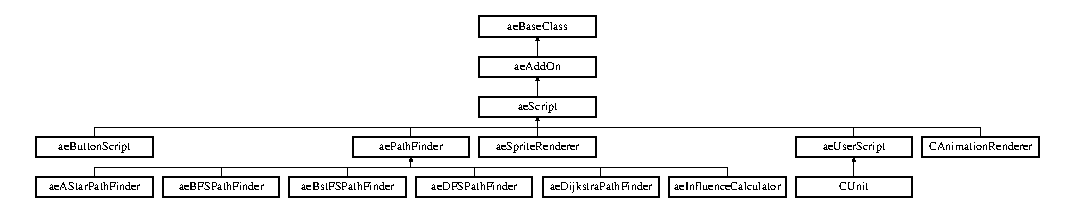
\includegraphics[height=2.430556cm]{classae_script}
\end{center}
\end{figure}
\subsection*{Public Member Functions}
\begin{DoxyCompactItemize}
\item 
\hyperlink{_scripts_8h_a5d3f231722ed23af7cf63216ade194f4}{Script\+Id} \hyperlink{classae_script_a4c7148b3f1a9ef7bda547670ead77acb}{Get\+Script\+Id} ()
\begin{DoxyCompactList}\small\item\em Gets script identifier. \end{DoxyCompactList}\end{DoxyCompactItemize}
\subsection*{Protected Attributes}
\begin{DoxyCompactItemize}
\item 
\hyperlink{_scripts_8h_a5d3f231722ed23af7cf63216ade194f4}{Script\+Id} {\bfseries m\+\_\+n\+Script\+ID}\hypertarget{classae_script_a171079568b73728009ecf964a8196f5c}{}\label{classae_script_a171079568b73728009ecf964a8196f5c}

\end{DoxyCompactItemize}


\subsection{Detailed Description}
A script. 

\subsection{Member Function Documentation}
\index{ae\+Script@{ae\+Script}!Get\+Script\+Id@{Get\+Script\+Id}}
\index{Get\+Script\+Id@{Get\+Script\+Id}!ae\+Script@{ae\+Script}}
\subsubsection[{\texorpdfstring{Get\+Script\+Id()}{GetScriptId()}}]{\setlength{\rightskip}{0pt plus 5cm}{\bf Script\+Id} ae\+Script\+::\+Get\+Script\+Id (
\begin{DoxyParamCaption}
{}
\end{DoxyParamCaption}
)}\hypertarget{classae_script_a4c7148b3f1a9ef7bda547670ead77acb}{}\label{classae_script_a4c7148b3f1a9ef7bda547670ead77acb}


Gets script identifier. 

\begin{DoxyReturn}{Returns}
The script identifier. 
\end{DoxyReturn}


The documentation for this class was generated from the following files\+:\begin{DoxyCompactItemize}
\item 
C\+:/\+Users/\+Alvaro Estrada/\+Documents/\+Visual Studio 2015/\+Projects/\+R\+T\+S\+\_\+\+A\+E/\+R\+T\+S\+\_\+\+A\+E/\+Game/\hyperlink{_scripts_8h}{Scripts.\+h}\item 
C\+:/\+Users/\+Alvaro Estrada/\+Documents/\+Visual Studio 2015/\+Projects/\+R\+T\+S\+\_\+\+A\+E/\+R\+T\+S\+\_\+\+A\+E/\+Game/Scripts.\+cpp\end{DoxyCompactItemize}

\hypertarget{classae_core_1_1ae_sprite}{}\section{ae\+Core\+:\+:ae\+Sprite Class Reference}
\label{classae_core_1_1ae_sprite}\index{ae\+Core\+::ae\+Sprite@{ae\+Core\+::ae\+Sprite}}


This class reads and displays images given by the user.  




{\ttfamily \#include $<$Sprite.\+h$>$}

\subsection*{Public Member Functions}
\begin{DoxyCompactItemize}
\item 
\hyperlink{classae_core_1_1ae_sprite_af0831df244e64f7286384f7505e263d9}{ae\+Sprite} ()\hypertarget{classae_core_1_1ae_sprite_af0831df244e64f7286384f7505e263d9}{}\label{classae_core_1_1ae_sprite_af0831df244e64f7286384f7505e263d9}

\begin{DoxyCompactList}\small\item\em Default constructor. \end{DoxyCompactList}\item 
\hyperlink{classae_core_1_1ae_sprite_abae79605805258977e20e0dd4e86e2f4}{$\sim$ae\+Sprite} ()\hypertarget{classae_core_1_1ae_sprite_abae79605805258977e20e0dd4e86e2f4}{}\label{classae_core_1_1ae_sprite_abae79605805258977e20e0dd4e86e2f4}

\begin{DoxyCompactList}\small\item\em Destructor. \end{DoxyCompactList}\item 
bool \hyperlink{classae_core_1_1ae_sprite_a47c5c7900491b50bc27e0ff4f9604612}{Load\+Image\+From\+File} (\hyperlink{namespaceae_core_ad6f85aacc0d1fdd85e458e2413e60010}{ae\+String} psz\+File\+Name, \hyperlink{classae_core_1_1ae_renderer}{ae\+Renderer} $\ast$p\+Renderer)
\begin{DoxyCompactList}\small\item\em Loads image from file. \end{DoxyCompactList}\item 
bool \hyperlink{classae_core_1_1ae_sprite_a78a94a3b8e133c094935ef37470d2c43}{Load\+Image\+From\+Text} (\hyperlink{classae_core_1_1ae_renderer}{ae\+Renderer} $\ast$p\+Renderer, \hyperlink{classae_core_1_1ae_font}{ae\+Font} $\ast$p\+Font, \hyperlink{namespaceae_core_ad6f85aacc0d1fdd85e458e2413e60010}{ae\+String} \&psz\+Text, int Size)
\begin{DoxyCompactList}\small\item\em Loads image from text. \end{DoxyCompactList}\item 
void \hyperlink{classae_core_1_1ae_sprite_a40fc5810e02f0314c4005e1b28164389}{Free} ()\hypertarget{classae_core_1_1ae_sprite_a40fc5810e02f0314c4005e1b28164389}{}\label{classae_core_1_1ae_sprite_a40fc5810e02f0314c4005e1b28164389}

\begin{DoxyCompactList}\small\item\em Frees this object. \end{DoxyCompactList}\item 
void \hyperlink{classae_core_1_1ae_sprite_aad4b4308c569dadfed99de71bd921978}{Set\+Color} (\hyperlink{structae_core_1_1ae_r_g_b}{ae\+R\+GB} rgb\+Color)
\begin{DoxyCompactList}\small\item\em Sets a color. \end{DoxyCompactList}\item 
void \hyperlink{classae_core_1_1ae_sprite_ad980068b083f6fc02cb87d8be4fa40f5}{Set\+Blend\+Mode} (int blending)
\begin{DoxyCompactList}\small\item\em Sets blend mode. \end{DoxyCompactList}\item 
void \hyperlink{classae_core_1_1ae_sprite_a926c9e48628fbc48eb5566d4ed61e474}{Set\+Alpha} (\hyperlink{namespaceae_core_aa13093dc911869e5b24942552898f01f}{uint8} alpha)
\begin{DoxyCompactList}\small\item\em Sets an alpha. \end{DoxyCompactList}\item 
void \hyperlink{classae_core_1_1ae_sprite_a192f6b1813ee98b22ddbba28a81406d3}{Render} (\hyperlink{classae_core_1_1ae_renderer}{ae\+Renderer} $\ast$Renderer, int x, int y, \hyperlink{structae_core_1_1ae_point}{ae\+Point} $\ast$p\+Size=N\+U\+LL, \hyperlink{structae_core_1_1ae_rect}{ae\+Rect} $\ast$p\+Rect\+Source=N\+U\+LL)
\begin{DoxyCompactList}\small\item\em Renders this object. \end{DoxyCompactList}\item 
void \hyperlink{classae_core_1_1ae_sprite_a369bf559adcd3e29b0afd99c24db5b3f}{Render\+Ex} (\hyperlink{classae_core_1_1ae_renderer}{ae\+Renderer} $\ast$Renderer, int x, int y, \hyperlink{structae_core_1_1ae_point}{ae\+Point} $\ast$p\+Size=N\+U\+LL, \hyperlink{structae_core_1_1ae_rect}{ae\+Rect} $\ast$p\+Rect\+Source=N\+U\+LL, int Flip=0, \hyperlink{structae_core_1_1ae_point}{ae\+Point} $\ast$p\+Center=N\+U\+LL, float Angle=0.\+0f)
\begin{DoxyCompactList}\small\item\em Renders this object. \end{DoxyCompactList}\item 
int \hyperlink{classae_core_1_1ae_sprite_aaaec389bd44191ed8796fa75373a402b}{Height} ()
\begin{DoxyCompactList}\small\item\em Gets the height. \end{DoxyCompactList}\item 
int \hyperlink{classae_core_1_1ae_sprite_a311d1c6b6dc0fe388f46ca46905f28a6}{Width} ()
\begin{DoxyCompactList}\small\item\em Gets the width. \end{DoxyCompactList}\item 
\hyperlink{structae_core_1_1ae_point}{ae\+Point} \hyperlink{classae_core_1_1ae_sprite_ad46bd4ad56230400d629fa05211d2b10}{Get\+Size} ()
\begin{DoxyCompactList}\small\item\em Gets the size. \end{DoxyCompactList}\item 
int \hyperlink{classae_core_1_1ae_sprite_adcef90ab9c0eb35dbe3386ac81de7e1f}{Get\+ID} ()
\begin{DoxyCompactList}\small\item\em Gets the identifier. \end{DoxyCompactList}\item 
void \hyperlink{classae_core_1_1ae_sprite_ab5aa44b474a501f757ad446a292fa5aa}{Set\+As\+Render\+Target} (\hyperlink{classae_core_1_1ae_renderer}{ae\+Renderer} $\ast$p\+Renderer, int w, int h)
\begin{DoxyCompactList}\small\item\em Sets as render target. \end{DoxyCompactList}\end{DoxyCompactItemize}
\subsection*{Static Public Member Functions}
\begin{DoxyCompactItemize}
\item 
static \hyperlink{classae_core_1_1ae_sprite}{ae\+Sprite} $\ast$ \hyperlink{classae_core_1_1ae_sprite_a21ae55423867b80c2e8db783cfdbaad6}{Create\+Sprite} (\hyperlink{namespaceae_core_ad6f85aacc0d1fdd85e458e2413e60010}{ae\+String} psz\+Path, \hyperlink{namespaceae_core_ad6f85aacc0d1fdd85e458e2413e60010}{ae\+String} psz\+Name, \hyperlink{classae_core_1_1ae_renderer}{ae\+Renderer} $\ast$p\+Renderer, int ID)
\begin{DoxyCompactList}\small\item\em Creates a sprite. \end{DoxyCompactList}\item 
static \hyperlink{classae_core_1_1ae_sprite}{ae\+Sprite} $\ast$ \hyperlink{classae_core_1_1ae_sprite_addce4be06369bd7996a06f279292329c}{Create\+Target\+Renderer} (\hyperlink{classae_core_1_1ae_renderer}{ae\+Renderer} $\ast$p\+Renderer, int w, int h)
\begin{DoxyCompactList}\small\item\em Creates target renderer. \end{DoxyCompactList}\item 
static \hyperlink{classae_core_1_1ae_sprite}{ae\+Sprite} $\ast$ \hyperlink{classae_core_1_1ae_sprite_a12ba14c6c0c3a429334faee5ce9ff23f}{Create\+Text\+Image} (\hyperlink{classae_core_1_1ae_renderer}{ae\+Renderer} $\ast$p\+Renderer, \hyperlink{classae_core_1_1ae_font}{ae\+Font} $\ast$p\+Font, \hyperlink{namespaceae_core_ad6f85aacc0d1fdd85e458e2413e60010}{ae\+String} \&psz\+Text, int Size)
\begin{DoxyCompactList}\small\item\em Creates an image from text. \end{DoxyCompactList}\end{DoxyCompactItemize}
\subsection*{Public Attributes}
\begin{DoxyCompactItemize}
\item 
\hyperlink{namespaceae_core_ad6f85aacc0d1fdd85e458e2413e60010}{ae\+String} {\bfseries Name}\hypertarget{classae_core_1_1ae_sprite_aef9b53797a7e7f79533b59b69f5957fb}{}\label{classae_core_1_1ae_sprite_aef9b53797a7e7f79533b59b69f5957fb}

\end{DoxyCompactItemize}
\subsection*{Friends}
\begin{DoxyCompactItemize}
\item 
class {\bfseries ae\+Renderer}\hypertarget{classae_core_1_1ae_sprite_a49b84ec66b2f0146e385d8f4982f4875}{}\label{classae_core_1_1ae_sprite_a49b84ec66b2f0146e385d8f4982f4875}

\end{DoxyCompactItemize}


\subsection{Detailed Description}
This class reads and displays images given by the user. 

\subsection{Member Function Documentation}
\index{ae\+Core\+::ae\+Sprite@{ae\+Core\+::ae\+Sprite}!Create\+Sprite@{Create\+Sprite}}
\index{Create\+Sprite@{Create\+Sprite}!ae\+Core\+::ae\+Sprite@{ae\+Core\+::ae\+Sprite}}
\subsubsection[{\texorpdfstring{Create\+Sprite(ae\+String psz\+Path, ae\+String psz\+Name, ae\+Renderer $\ast$p\+Renderer, int I\+D)}{CreateSprite(aeString pszPath, aeString pszName, aeRenderer *pRenderer, int ID)}}]{\setlength{\rightskip}{0pt plus 5cm}static {\bf ae\+Sprite} $\ast$ ae\+Core\+::ae\+Sprite\+::\+Create\+Sprite (
\begin{DoxyParamCaption}
\item[{{\bf ae\+String}}]{psz\+Path, }
\item[{{\bf ae\+String}}]{psz\+Name, }
\item[{{\bf ae\+Renderer} $\ast$}]{p\+Renderer, }
\item[{int}]{ID}
\end{DoxyParamCaption}
)\hspace{0.3cm}{\ttfamily [static]}}\hypertarget{classae_core_1_1ae_sprite_a21ae55423867b80c2e8db783cfdbaad6}{}\label{classae_core_1_1ae_sprite_a21ae55423867b80c2e8db783cfdbaad6}


Creates a sprite. 


\begin{DoxyParams}[1]{Parameters}
 & {\em psz\+Path} & Path of the file. \\
\hline
 & {\em psz\+Name} & The name. \\
\hline
\mbox{\tt in,out}  & {\em p\+Renderer} & If non-\/null, the renderer. \\
\hline
 & {\em ID} & If non-\/null, the transaction color.\\
\hline
\end{DoxyParams}
\begin{DoxyReturn}{Returns}
The new sprite.
\end{DoxyReturn}

\begin{DoxyParams}[1]{Parameters}
 & {\em psz\+Path} & Path of the file. \\
\hline
 & {\em psz\+Name} & The name. \\
\hline
\mbox{\tt in,out}  & {\em p\+Renderer} & If non-\/null, the renderer. \\
\hline
 & {\em ID} & The identifier.\\
\hline
\end{DoxyParams}
\begin{DoxyReturn}{Returns}
The new sprite. 
\end{DoxyReturn}
\index{ae\+Core\+::ae\+Sprite@{ae\+Core\+::ae\+Sprite}!Create\+Target\+Renderer@{Create\+Target\+Renderer}}
\index{Create\+Target\+Renderer@{Create\+Target\+Renderer}!ae\+Core\+::ae\+Sprite@{ae\+Core\+::ae\+Sprite}}
\subsubsection[{\texorpdfstring{Create\+Target\+Renderer(ae\+Renderer $\ast$p\+Renderer, int w, int h)}{CreateTargetRenderer(aeRenderer *pRenderer, int w, int h)}}]{\setlength{\rightskip}{0pt plus 5cm}static {\bf ae\+Sprite} $\ast$ ae\+Core\+::ae\+Sprite\+::\+Create\+Target\+Renderer (
\begin{DoxyParamCaption}
\item[{{\bf ae\+Renderer} $\ast$}]{p\+Renderer, }
\item[{int}]{w, }
\item[{int}]{h}
\end{DoxyParamCaption}
)\hspace{0.3cm}{\ttfamily [static]}}\hypertarget{classae_core_1_1ae_sprite_addce4be06369bd7996a06f279292329c}{}\label{classae_core_1_1ae_sprite_addce4be06369bd7996a06f279292329c}


Creates target renderer. 


\begin{DoxyParams}[1]{Parameters}
\mbox{\tt in,out}  & {\em p\+Renderer} & If non-\/null, the renderer. \\
\hline
 & {\em w} & The width. \\
\hline
 & {\em h} & The height.\\
\hline
\end{DoxyParams}
\begin{DoxyReturn}{Returns}
null if it fails, else the new target renderer. 
\end{DoxyReturn}
\index{ae\+Core\+::ae\+Sprite@{ae\+Core\+::ae\+Sprite}!Create\+Text\+Image@{Create\+Text\+Image}}
\index{Create\+Text\+Image@{Create\+Text\+Image}!ae\+Core\+::ae\+Sprite@{ae\+Core\+::ae\+Sprite}}
\subsubsection[{\texorpdfstring{Create\+Text\+Image(ae\+Renderer $\ast$p\+Renderer, ae\+Font $\ast$p\+Font, ae\+String \&psz\+Text, int Size)}{CreateTextImage(aeRenderer *pRenderer, aeFont *pFont, aeString &pszText, int Size)}}]{\setlength{\rightskip}{0pt plus 5cm}static {\bf ae\+Sprite} $\ast$ ae\+Core\+::ae\+Sprite\+::\+Create\+Text\+Image (
\begin{DoxyParamCaption}
\item[{{\bf ae\+Renderer} $\ast$}]{p\+Renderer, }
\item[{{\bf ae\+Font} $\ast$}]{p\+Font, }
\item[{{\bf ae\+String} \&}]{psz\+Text, }
\item[{int}]{Size}
\end{DoxyParamCaption}
)\hspace{0.3cm}{\ttfamily [static]}}\hypertarget{classae_core_1_1ae_sprite_a12ba14c6c0c3a429334faee5ce9ff23f}{}\label{classae_core_1_1ae_sprite_a12ba14c6c0c3a429334faee5ce9ff23f}


Creates an image from text. 


\begin{DoxyParams}[1]{Parameters}
\mbox{\tt in,out}  & {\em p\+Renderer} & If non-\/null, the renderer. \\
\hline
\mbox{\tt in,out}  & {\em p\+Font} & If non-\/null, the font. \\
\hline
\mbox{\tt in,out}  & {\em psz\+Text} & The text. \\
\hline
 & {\em Size} & The size.\\
\hline
\end{DoxyParams}
\begin{DoxyReturn}{Returns}
null if it fails, else the new text image. 
\end{DoxyReturn}
\index{ae\+Core\+::ae\+Sprite@{ae\+Core\+::ae\+Sprite}!Get\+ID@{Get\+ID}}
\index{Get\+ID@{Get\+ID}!ae\+Core\+::ae\+Sprite@{ae\+Core\+::ae\+Sprite}}
\subsubsection[{\texorpdfstring{Get\+I\+D()}{GetID()}}]{\setlength{\rightskip}{0pt plus 5cm}int ae\+Core\+::ae\+Sprite\+::\+Get\+ID (
\begin{DoxyParamCaption}
{}
\end{DoxyParamCaption}
)}\hypertarget{classae_core_1_1ae_sprite_adcef90ab9c0eb35dbe3386ac81de7e1f}{}\label{classae_core_1_1ae_sprite_adcef90ab9c0eb35dbe3386ac81de7e1f}


Gets the identifier. 

\begin{DoxyReturn}{Returns}
The identifier. 
\end{DoxyReturn}
\index{ae\+Core\+::ae\+Sprite@{ae\+Core\+::ae\+Sprite}!Get\+Size@{Get\+Size}}
\index{Get\+Size@{Get\+Size}!ae\+Core\+::ae\+Sprite@{ae\+Core\+::ae\+Sprite}}
\subsubsection[{\texorpdfstring{Get\+Size()}{GetSize()}}]{\setlength{\rightskip}{0pt plus 5cm}{\bf ae\+Point} ae\+Core\+::ae\+Sprite\+::\+Get\+Size (
\begin{DoxyParamCaption}
{}
\end{DoxyParamCaption}
)}\hypertarget{classae_core_1_1ae_sprite_ad46bd4ad56230400d629fa05211d2b10}{}\label{classae_core_1_1ae_sprite_ad46bd4ad56230400d629fa05211d2b10}


Gets the size. 

\begin{DoxyReturn}{Returns}
The size. 
\end{DoxyReturn}
\index{ae\+Core\+::ae\+Sprite@{ae\+Core\+::ae\+Sprite}!Height@{Height}}
\index{Height@{Height}!ae\+Core\+::ae\+Sprite@{ae\+Core\+::ae\+Sprite}}
\subsubsection[{\texorpdfstring{Height()}{Height()}}]{\setlength{\rightskip}{0pt plus 5cm}int ae\+Core\+::ae\+Sprite\+::\+Height (
\begin{DoxyParamCaption}
{}
\end{DoxyParamCaption}
)}\hypertarget{classae_core_1_1ae_sprite_aaaec389bd44191ed8796fa75373a402b}{}\label{classae_core_1_1ae_sprite_aaaec389bd44191ed8796fa75373a402b}


Gets the height. 

\begin{DoxyReturn}{Returns}
An int. 
\end{DoxyReturn}
\index{ae\+Core\+::ae\+Sprite@{ae\+Core\+::ae\+Sprite}!Load\+Image\+From\+File@{Load\+Image\+From\+File}}
\index{Load\+Image\+From\+File@{Load\+Image\+From\+File}!ae\+Core\+::ae\+Sprite@{ae\+Core\+::ae\+Sprite}}
\subsubsection[{\texorpdfstring{Load\+Image\+From\+File(ae\+String psz\+File\+Name, ae\+Renderer $\ast$p\+Renderer)}{LoadImageFromFile(aeString pszFileName, aeRenderer *pRenderer)}}]{\setlength{\rightskip}{0pt plus 5cm}bool ae\+Core\+::ae\+Sprite\+::\+Load\+Image\+From\+File (
\begin{DoxyParamCaption}
\item[{{\bf ae\+String}}]{psz\+File\+Name, }
\item[{{\bf ae\+Renderer} $\ast$}]{p\+Renderer}
\end{DoxyParamCaption}
)}\hypertarget{classae_core_1_1ae_sprite_a47c5c7900491b50bc27e0ff4f9604612}{}\label{classae_core_1_1ae_sprite_a47c5c7900491b50bc27e0ff4f9604612}


Loads image from file. 


\begin{DoxyParams}[1]{Parameters}
 & {\em psz\+File\+Name} & Filename of the file. \\
\hline
\mbox{\tt in,out}  & {\em p\+Renderer} & If non-\/null, the renderer.\\
\hline
\end{DoxyParams}
\begin{DoxyReturn}{Returns}
true if it succeeds, false if it fails. 
\end{DoxyReturn}
\index{ae\+Core\+::ae\+Sprite@{ae\+Core\+::ae\+Sprite}!Load\+Image\+From\+Text@{Load\+Image\+From\+Text}}
\index{Load\+Image\+From\+Text@{Load\+Image\+From\+Text}!ae\+Core\+::ae\+Sprite@{ae\+Core\+::ae\+Sprite}}
\subsubsection[{\texorpdfstring{Load\+Image\+From\+Text(ae\+Renderer $\ast$p\+Renderer, ae\+Font $\ast$p\+Font, ae\+String \&psz\+Text, int Size)}{LoadImageFromText(aeRenderer *pRenderer, aeFont *pFont, aeString &pszText, int Size)}}]{\setlength{\rightskip}{0pt plus 5cm}bool ae\+Core\+::ae\+Sprite\+::\+Load\+Image\+From\+Text (
\begin{DoxyParamCaption}
\item[{{\bf ae\+Renderer} $\ast$}]{p\+Renderer, }
\item[{{\bf ae\+Font} $\ast$}]{p\+Font, }
\item[{{\bf ae\+String} \&}]{psz\+Text, }
\item[{int}]{Size}
\end{DoxyParamCaption}
)}\hypertarget{classae_core_1_1ae_sprite_a78a94a3b8e133c094935ef37470d2c43}{}\label{classae_core_1_1ae_sprite_a78a94a3b8e133c094935ef37470d2c43}


Loads image from text. 


\begin{DoxyParams}[1]{Parameters}
\mbox{\tt in,out}  & {\em p\+Renderer} & If non-\/null, the renderer. \\
\hline
\mbox{\tt in,out}  & {\em p\+Font} & If non-\/null, the font. \\
\hline
\mbox{\tt in,out}  & {\em psz\+Text} & The text. \\
\hline
 & {\em Size} & The size.\\
\hline
\end{DoxyParams}
\begin{DoxyReturn}{Returns}
true if it succeeds, false if it fails. 
\end{DoxyReturn}
\index{ae\+Core\+::ae\+Sprite@{ae\+Core\+::ae\+Sprite}!Render@{Render}}
\index{Render@{Render}!ae\+Core\+::ae\+Sprite@{ae\+Core\+::ae\+Sprite}}
\subsubsection[{\texorpdfstring{Render(ae\+Renderer $\ast$\+Renderer, int x, int y, ae\+Point $\ast$p\+Size=\+N\+U\+L\+L, ae\+Rect $\ast$p\+Rect\+Source=\+N\+U\+L\+L)}{Render(aeRenderer *Renderer, int x, int y, aePoint *pSize=NULL, aeRect *pRectSource=NULL)}}]{\setlength{\rightskip}{0pt plus 5cm}void ae\+Core\+::ae\+Sprite\+::\+Render (
\begin{DoxyParamCaption}
\item[{{\bf ae\+Renderer} $\ast$}]{Renderer, }
\item[{int}]{x, }
\item[{int}]{y, }
\item[{{\bf ae\+Point} $\ast$}]{p\+Size = {\ttfamily NULL}, }
\item[{{\bf ae\+Rect} $\ast$}]{p\+Rect\+Source = {\ttfamily NULL}}
\end{DoxyParamCaption}
)}\hypertarget{classae_core_1_1ae_sprite_a192f6b1813ee98b22ddbba28a81406d3}{}\label{classae_core_1_1ae_sprite_a192f6b1813ee98b22ddbba28a81406d3}


Renders this object. 


\begin{DoxyParams}[1]{Parameters}
\mbox{\tt in,out}  & {\em Renderer} & The renderer. \\
\hline
 & {\em x} & The x coordinate. \\
\hline
 & {\em y} & The y coordinate. \\
\hline
\mbox{\tt in,out}  & {\em p\+Size} & If non-\/null, the size. \\
\hline
\mbox{\tt in,out}  & {\em p\+Rect\+Source} & If non-\/null, the rectangle source.\\
\hline
\mbox{\tt in,out}  & {\em Renderer} & If non-\/null, the renderer. \\
\hline
 & {\em x} & The x coordinate. \\
\hline
 & {\em y} & The y coordinate. \\
\hline
\mbox{\tt in,out}  & {\em p\+Size} & (Optional) If non-\/null, the size. \\
\hline
\mbox{\tt in,out}  & {\em p\+Rect\+Source} & (Optional) If non-\/null, the rectangle source. \\
\hline
\end{DoxyParams}
\index{ae\+Core\+::ae\+Sprite@{ae\+Core\+::ae\+Sprite}!Render\+Ex@{Render\+Ex}}
\index{Render\+Ex@{Render\+Ex}!ae\+Core\+::ae\+Sprite@{ae\+Core\+::ae\+Sprite}}
\subsubsection[{\texorpdfstring{Render\+Ex(ae\+Renderer $\ast$\+Renderer, int x, int y, ae\+Point $\ast$p\+Size=\+N\+U\+L\+L, ae\+Rect $\ast$p\+Rect\+Source=\+N\+U\+L\+L, int Flip=0, ae\+Point $\ast$p\+Center=\+N\+U\+L\+L, float Angle=0.\+0f)}{RenderEx(aeRenderer *Renderer, int x, int y, aePoint *pSize=NULL, aeRect *pRectSource=NULL, int Flip=0, aePoint *pCenter=NULL, float Angle=0.0f)}}]{\setlength{\rightskip}{0pt plus 5cm}void ae\+Core\+::ae\+Sprite\+::\+Render\+Ex (
\begin{DoxyParamCaption}
\item[{{\bf ae\+Renderer} $\ast$}]{Renderer, }
\item[{int}]{x, }
\item[{int}]{y, }
\item[{{\bf ae\+Point} $\ast$}]{p\+Size = {\ttfamily NULL}, }
\item[{{\bf ae\+Rect} $\ast$}]{p\+Rect\+Source = {\ttfamily NULL}, }
\item[{int}]{Flip = {\ttfamily 0}, }
\item[{{\bf ae\+Point} $\ast$}]{p\+Center = {\ttfamily NULL}, }
\item[{float}]{Angle = {\ttfamily 0.0f}}
\end{DoxyParamCaption}
)}\hypertarget{classae_core_1_1ae_sprite_a369bf559adcd3e29b0afd99c24db5b3f}{}\label{classae_core_1_1ae_sprite_a369bf559adcd3e29b0afd99c24db5b3f}


Renders this object. 


\begin{DoxyParams}[1]{Parameters}
\mbox{\tt in,out}  & {\em Renderer} & The renderer. \\
\hline
 & {\em x} & The x coordinate. \\
\hline
 & {\em y} & The y coordinate. \\
\hline
\mbox{\tt in,out}  & {\em p\+Size} & If non-\/null, the size. \\
\hline
\mbox{\tt in,out}  & {\em p\+Rect\+Source} & If non-\/null, the rectangle source. \\
\hline
\mbox{\tt in,out}  & {\em p\+Center} & If non-\/null, the center. \\
\hline
 & {\em Flip} & The flip. \\
\hline
 & {\em Angle} & The angle.\\
\hline
\mbox{\tt in,out}  & {\em Renderer} & If non-\/null, the renderer. \\
\hline
 & {\em x} & The x coordinate. \\
\hline
 & {\em y} & The y coordinate. \\
\hline
\mbox{\tt in,out}  & {\em p\+Size} & (Optional) If non-\/null, the size. \\
\hline
\mbox{\tt in,out}  & {\em p\+Rect\+Source} & (Optional) If non-\/null, the rectangle source. \\
\hline
 & {\em Flip} & The flip. \\
\hline
\mbox{\tt in,out}  & {\em p\+Center} & (Optional) If non-\/null, the center. \\
\hline
 & {\em Angle} & The angle. \\
\hline
\end{DoxyParams}
\index{ae\+Core\+::ae\+Sprite@{ae\+Core\+::ae\+Sprite}!Set\+Alpha@{Set\+Alpha}}
\index{Set\+Alpha@{Set\+Alpha}!ae\+Core\+::ae\+Sprite@{ae\+Core\+::ae\+Sprite}}
\subsubsection[{\texorpdfstring{Set\+Alpha(uint8 alpha)}{SetAlpha(uint8 alpha)}}]{\setlength{\rightskip}{0pt plus 5cm}void ae\+Core\+::ae\+Sprite\+::\+Set\+Alpha (
\begin{DoxyParamCaption}
\item[{{\bf uint8}}]{alpha}
\end{DoxyParamCaption}
)}\hypertarget{classae_core_1_1ae_sprite_a926c9e48628fbc48eb5566d4ed61e474}{}\label{classae_core_1_1ae_sprite_a926c9e48628fbc48eb5566d4ed61e474}


Sets an alpha. 


\begin{DoxyParams}{Parameters}
{\em alpha} & The alpha. \\
\hline
\end{DoxyParams}
\index{ae\+Core\+::ae\+Sprite@{ae\+Core\+::ae\+Sprite}!Set\+As\+Render\+Target@{Set\+As\+Render\+Target}}
\index{Set\+As\+Render\+Target@{Set\+As\+Render\+Target}!ae\+Core\+::ae\+Sprite@{ae\+Core\+::ae\+Sprite}}
\subsubsection[{\texorpdfstring{Set\+As\+Render\+Target(ae\+Renderer $\ast$p\+Renderer, int w, int h)}{SetAsRenderTarget(aeRenderer *pRenderer, int w, int h)}}]{\setlength{\rightskip}{0pt plus 5cm}void ae\+Core\+::ae\+Sprite\+::\+Set\+As\+Render\+Target (
\begin{DoxyParamCaption}
\item[{{\bf ae\+Renderer} $\ast$}]{p\+Renderer, }
\item[{int}]{w, }
\item[{int}]{h}
\end{DoxyParamCaption}
)}\hypertarget{classae_core_1_1ae_sprite_ab5aa44b474a501f757ad446a292fa5aa}{}\label{classae_core_1_1ae_sprite_ab5aa44b474a501f757ad446a292fa5aa}


Sets as render target. 


\begin{DoxyParams}[1]{Parameters}
\mbox{\tt in,out}  & {\em p\+Renderer} & If non-\/null, the renderer. \\
\hline
 & {\em w} & The width. \\
\hline
 & {\em h} & The height. \\
\hline
\end{DoxyParams}
\index{ae\+Core\+::ae\+Sprite@{ae\+Core\+::ae\+Sprite}!Set\+Blend\+Mode@{Set\+Blend\+Mode}}
\index{Set\+Blend\+Mode@{Set\+Blend\+Mode}!ae\+Core\+::ae\+Sprite@{ae\+Core\+::ae\+Sprite}}
\subsubsection[{\texorpdfstring{Set\+Blend\+Mode(int blending)}{SetBlendMode(int blending)}}]{\setlength{\rightskip}{0pt plus 5cm}void ae\+Core\+::ae\+Sprite\+::\+Set\+Blend\+Mode (
\begin{DoxyParamCaption}
\item[{int}]{blending}
\end{DoxyParamCaption}
)}\hypertarget{classae_core_1_1ae_sprite_ad980068b083f6fc02cb87d8be4fa40f5}{}\label{classae_core_1_1ae_sprite_ad980068b083f6fc02cb87d8be4fa40f5}


Sets blend mode. 


\begin{DoxyParams}{Parameters}
{\em blending} & The blending. \\
\hline
\end{DoxyParams}
\index{ae\+Core\+::ae\+Sprite@{ae\+Core\+::ae\+Sprite}!Set\+Color@{Set\+Color}}
\index{Set\+Color@{Set\+Color}!ae\+Core\+::ae\+Sprite@{ae\+Core\+::ae\+Sprite}}
\subsubsection[{\texorpdfstring{Set\+Color(ae\+R\+G\+B rgb\+Color)}{SetColor(aeRGB rgbColor)}}]{\setlength{\rightskip}{0pt plus 5cm}void ae\+Core\+::ae\+Sprite\+::\+Set\+Color (
\begin{DoxyParamCaption}
\item[{{\bf ae\+R\+GB}}]{rgb\+Color}
\end{DoxyParamCaption}
)}\hypertarget{classae_core_1_1ae_sprite_aad4b4308c569dadfed99de71bd921978}{}\label{classae_core_1_1ae_sprite_aad4b4308c569dadfed99de71bd921978}


Sets a color. 

Sets a color modifier.


\begin{DoxyParams}{Parameters}
{\em rgb\+Color} & The R\+GB color. \\
\hline
\end{DoxyParams}
\index{ae\+Core\+::ae\+Sprite@{ae\+Core\+::ae\+Sprite}!Width@{Width}}
\index{Width@{Width}!ae\+Core\+::ae\+Sprite@{ae\+Core\+::ae\+Sprite}}
\subsubsection[{\texorpdfstring{Width()}{Width()}}]{\setlength{\rightskip}{0pt plus 5cm}int ae\+Core\+::ae\+Sprite\+::\+Width (
\begin{DoxyParamCaption}
{}
\end{DoxyParamCaption}
)}\hypertarget{classae_core_1_1ae_sprite_a311d1c6b6dc0fe388f46ca46905f28a6}{}\label{classae_core_1_1ae_sprite_a311d1c6b6dc0fe388f46ca46905f28a6}


Gets the width. 

\begin{DoxyReturn}{Returns}
An int. 
\end{DoxyReturn}


The documentation for this class was generated from the following files\+:\begin{DoxyCompactItemize}
\item 
C\+:/\+Users/\+Alvaro Estrada/\+Documents/\+Visual Studio 2015/\+Projects/\+R\+T\+S\+\_\+\+A\+E/ae\+Core/\+Graphics/\hyperlink{_sprite_8h}{Sprite.\+h}\item 
C\+:/\+Users/\+Alvaro Estrada/\+Documents/\+Visual Studio 2015/\+Projects/\+R\+T\+S\+\_\+\+A\+E/ae\+Core/\+Graphics/\hyperlink{_sprite_8cpp}{Sprite.\+cpp}\end{DoxyCompactItemize}

\hypertarget{classae_sprite_renderer}{}\section{ae\+Sprite\+Renderer Class Reference}
\label{classae_sprite_renderer}\index{ae\+Sprite\+Renderer@{ae\+Sprite\+Renderer}}
Inheritance diagram for ae\+Sprite\+Renderer\+:\begin{figure}[H]
\begin{center}
\leavevmode
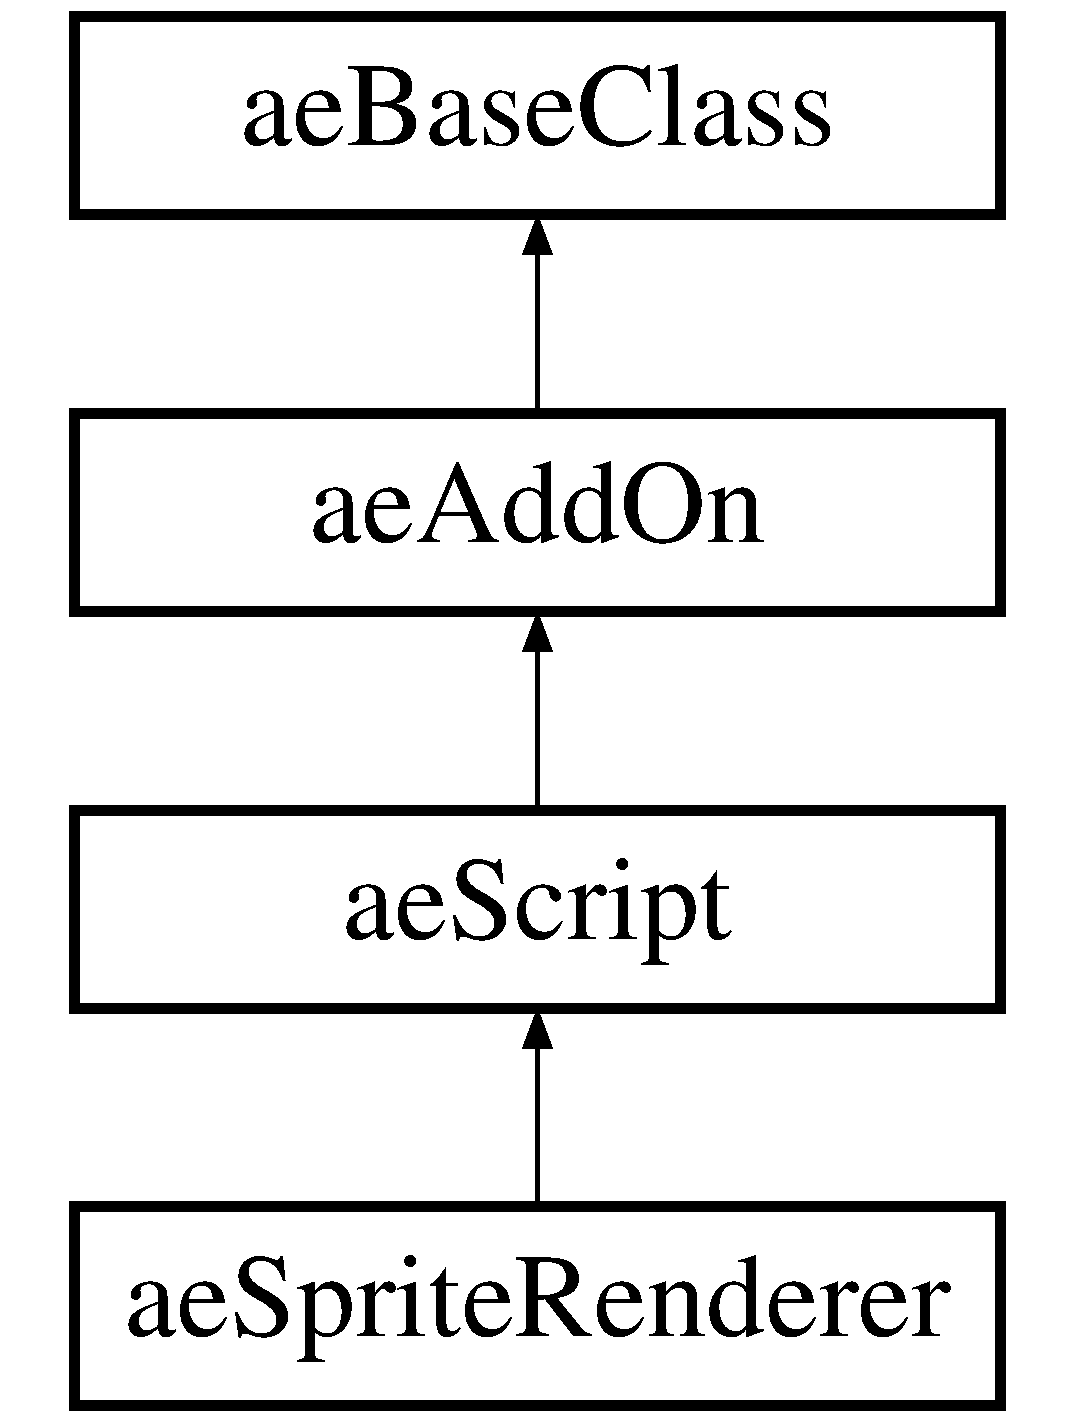
\includegraphics[height=4.000000cm]{classae_sprite_renderer}
\end{center}
\end{figure}
\subsection*{Public Member Functions}
\begin{DoxyCompactItemize}
\item 
virtual int \hyperlink{classae_sprite_renderer_a97a72a34026e64766a0ab4840376cd76}{Init} (\hyperlink{classae_base_class}{ae\+Base\+Class} $\ast$p\+Parent)
\begin{DoxyCompactList}\small\item\em Initializes with the given parent pointer. \end{DoxyCompactList}\item 
virtual void \hyperlink{classae_sprite_renderer_a65ea9a0ad3452271d2d5b8c140a7eff7}{Update} (float f\+Delta)
\begin{DoxyCompactList}\small\item\em Updates the given f\+Delta. \end{DoxyCompactList}\item 
virtual void \hyperlink{classae_sprite_renderer_a1583eea9478f23549cf9355091542d6a}{Render} (\hyperlink{classae_core_1_1ae_renderer}{ae\+Renderer} $\ast$p\+Renderer)
\begin{DoxyCompactList}\small\item\em Paints on the given renderer pointer. \end{DoxyCompactList}\item 
virtual void \hyperlink{classae_sprite_renderer_acba90289bfe989eda9480258fc679400}{Destroy} ()\hypertarget{classae_sprite_renderer_acba90289bfe989eda9480258fc679400}{}\label{classae_sprite_renderer_acba90289bfe989eda9480258fc679400}

\begin{DoxyCompactList}\small\item\em Destroys this object. \end{DoxyCompactList}\item 
virtual void {\bfseries Set\+Object} (void $\ast$Object)\hypertarget{classae_sprite_renderer_a398961d623fbcd4428a4f8ad815cf0b8}{}\label{classae_sprite_renderer_a398961d623fbcd4428a4f8ad815cf0b8}

\end{DoxyCompactItemize}
\subsection*{Public Attributes}
\begin{DoxyCompactItemize}
\item 
int {\bfseries Order\+Of\+Render}\hypertarget{classae_sprite_renderer_a8bd696b830181ba037adec7e828113a8}{}\label{classae_sprite_renderer_a8bd696b830181ba037adec7e828113a8}

\item 
bool {\bfseries MirrorX}\hypertarget{classae_sprite_renderer_ac8b2f24ff43bb93147073667349543ac}{}\label{classae_sprite_renderer_ac8b2f24ff43bb93147073667349543ac}

\item 
bool {\bfseries MirrorY}\hypertarget{classae_sprite_renderer_a31d66d0f5d6c282e2a96641fa64a5f99}{}\label{classae_sprite_renderer_a31d66d0f5d6c282e2a96641fa64a5f99}

\item 
ae\+Rect {\bfseries Render\+Rect}\hypertarget{classae_sprite_renderer_aabc1c57ae8819179dec0d55cee701b2e}{}\label{classae_sprite_renderer_aabc1c57ae8819179dec0d55cee701b2e}

\item 
ae\+Rect {\bfseries Source\+Rect}\hypertarget{classae_sprite_renderer_a796771afd1c08345e69f753e93da0b35}{}\label{classae_sprite_renderer_a796771afd1c08345e69f753e93da0b35}

\end{DoxyCompactItemize}
\subsection*{Additional Inherited Members}


\subsection{Member Function Documentation}
\index{ae\+Sprite\+Renderer@{ae\+Sprite\+Renderer}!Init@{Init}}
\index{Init@{Init}!ae\+Sprite\+Renderer@{ae\+Sprite\+Renderer}}
\subsubsection[{\texorpdfstring{Init(ae\+Base\+Class $\ast$p\+Parent)}{Init(aeBaseClass *pParent)}}]{\setlength{\rightskip}{0pt plus 5cm}int ae\+Sprite\+Renderer\+::\+Init (
\begin{DoxyParamCaption}
\item[{{\bf ae\+Base\+Class} $\ast$}]{p\+Parent}
\end{DoxyParamCaption}
)\hspace{0.3cm}{\ttfamily [virtual]}}\hypertarget{classae_sprite_renderer_a97a72a34026e64766a0ab4840376cd76}{}\label{classae_sprite_renderer_a97a72a34026e64766a0ab4840376cd76}


Initializes with the given parent pointer. 


\begin{DoxyParams}[1]{Parameters}
\mbox{\tt in,out}  & {\em p\+Parent} & If non-\/null, the parent pointer. \\
\hline
\end{DoxyParams}


Implements \hyperlink{classae_add_on_a0730c1446e548031f9a4e98435a54675}{ae\+Add\+On}.

\index{ae\+Sprite\+Renderer@{ae\+Sprite\+Renderer}!Render@{Render}}
\index{Render@{Render}!ae\+Sprite\+Renderer@{ae\+Sprite\+Renderer}}
\subsubsection[{\texorpdfstring{Render(ae\+Renderer $\ast$p\+Renderer)}{Render(aeRenderer *pRenderer)}}]{\setlength{\rightskip}{0pt plus 5cm}void ae\+Sprite\+Renderer\+::\+Render (
\begin{DoxyParamCaption}
\item[{{\bf ae\+Renderer} $\ast$}]{p\+Renderer}
\end{DoxyParamCaption}
)\hspace{0.3cm}{\ttfamily [virtual]}}\hypertarget{classae_sprite_renderer_a1583eea9478f23549cf9355091542d6a}{}\label{classae_sprite_renderer_a1583eea9478f23549cf9355091542d6a}


Paints on the given renderer pointer. 


\begin{DoxyParams}[1]{Parameters}
\mbox{\tt in,out}  & {\em p\+Renderer} & The renderer pointer. \\
\hline
\end{DoxyParams}


Reimplemented from \hyperlink{classae_add_on_ab6bed56009b9c92df8ae017a27587dc3}{ae\+Add\+On}.

\index{ae\+Sprite\+Renderer@{ae\+Sprite\+Renderer}!Update@{Update}}
\index{Update@{Update}!ae\+Sprite\+Renderer@{ae\+Sprite\+Renderer}}
\subsubsection[{\texorpdfstring{Update(float f\+Delta)}{Update(float fDelta)}}]{\setlength{\rightskip}{0pt plus 5cm}void ae\+Sprite\+Renderer\+::\+Update (
\begin{DoxyParamCaption}
\item[{float}]{f\+Delta}
\end{DoxyParamCaption}
)\hspace{0.3cm}{\ttfamily [virtual]}}\hypertarget{classae_sprite_renderer_a65ea9a0ad3452271d2d5b8c140a7eff7}{}\label{classae_sprite_renderer_a65ea9a0ad3452271d2d5b8c140a7eff7}


Updates the given f\+Delta. 


\begin{DoxyParams}{Parameters}
{\em f\+Delta} & The delta time. \\
\hline
\end{DoxyParams}


Implements \hyperlink{classae_add_on_a51caa4b8680206495ea671e71991e231}{ae\+Add\+On}.



The documentation for this class was generated from the following files\+:\begin{DoxyCompactItemize}
\item 
C\+:/\+Users/\+Alvaro Estrada/\+Documents/\+Visual Studio 2015/\+Projects/\+R\+T\+S\+\_\+\+A\+E/\+R\+T\+S\+\_\+\+A\+E/\+Game/Sprite\+Renderer.\+h\item 
C\+:/\+Users/\+Alvaro Estrada/\+Documents/\+Visual Studio 2015/\+Projects/\+R\+T\+S\+\_\+\+A\+E/\+R\+T\+S\+\_\+\+A\+E/\+Game/Sprite\+Renderer.\+cpp\end{DoxyCompactItemize}

\hypertarget{classae_core_1_1ae_s_q_l_connector}{}\section{ae\+Core\+:\+:ae\+S\+Q\+L\+Connector Class Reference}
\label{classae_core_1_1ae_s_q_l_connector}\index{ae\+Core\+::ae\+S\+Q\+L\+Connector@{ae\+Core\+::ae\+S\+Q\+L\+Connector}}


A S\+QL connector. This class purpose is to create a connection to the database using S\+QL commands.  




{\ttfamily \#include $<$S\+Q\+L\+Connector.\+h$>$}

\subsection*{Public Member Functions}
\begin{DoxyCompactItemize}
\item 
void \hyperlink{classae_core_1_1ae_s_q_l_connector_af604e8c8435901e15f496a76762f36b7}{Open\+Database} (const \hyperlink{namespaceae_core_a052c557709e5ab43db521b23085fd916}{T\+C\+H\+AR} $\ast$file\+\_\+name)
\begin{DoxyCompactList}\small\item\em Receives the file path or file name in case in the same carpet, opens the connection to the database to start making query requests. \end{DoxyCompactList}\item 
void \hyperlink{classae_core_1_1ae_s_q_l_connector_a4b5f3e5b93afe08ed5fa09e9e8f349ed}{Close\+Database} ()\hypertarget{classae_core_1_1ae_s_q_l_connector_a4b5f3e5b93afe08ed5fa09e9e8f349ed}{}\label{classae_core_1_1ae_s_q_l_connector_a4b5f3e5b93afe08ed5fa09e9e8f349ed}

\begin{DoxyCompactList}\small\item\em Closes the connection to the database. \end{DoxyCompactList}\item 
int \hyperlink{classae_core_1_1ae_s_q_l_connector_ac1d0350ad470ed0210039d6be34f3382}{Query\+Database} (const \hyperlink{namespaceae_core_a052c557709e5ab43db521b23085fd916}{T\+C\+H\+AR} $\ast$sql\+\_\+query, int($\ast$Query\+Callback)(void $\ast$, int, char $\ast$$\ast$, char $\ast$$\ast$), void $\ast$Non\+Static\+Object)
\begin{DoxyCompactList}\small\item\em Executes a query request of a list and passes along a function that executes per line of the list. \end{DoxyCompactList}\item 
int \hyperlink{classae_core_1_1ae_s_q_l_connector_afde051a9349eb109bd118abe87bfcb11}{Exec\+Statement} (const \hyperlink{namespaceae_core_a052c557709e5ab43db521b23085fd916}{T\+C\+H\+AR} $\ast$sql\+\_\+query, int Size)
\begin{DoxyCompactList}\small\item\em Executes any kind of query request, it receives the command and the length in characters of the command. \end{DoxyCompactList}\end{DoxyCompactItemize}


\subsection{Detailed Description}
A S\+QL connector. This class purpose is to create a connection to the database using S\+QL commands. 

\begin{DoxyAuthor}{Author}
Alvaro Estrada 
\end{DoxyAuthor}
\begin{DoxyDate}{Date}
14/05/2016 
\end{DoxyDate}


\subsection{Member Function Documentation}
\index{ae\+Core\+::ae\+S\+Q\+L\+Connector@{ae\+Core\+::ae\+S\+Q\+L\+Connector}!Exec\+Statement@{Exec\+Statement}}
\index{Exec\+Statement@{Exec\+Statement}!ae\+Core\+::ae\+S\+Q\+L\+Connector@{ae\+Core\+::ae\+S\+Q\+L\+Connector}}
\subsubsection[{\texorpdfstring{Exec\+Statement(const T\+C\+H\+A\+R $\ast$sql\+\_\+query, int Size)}{ExecStatement(const TCHAR *sql_query, int Size)}}]{\setlength{\rightskip}{0pt plus 5cm}int ae\+Core\+::ae\+S\+Q\+L\+Connector\+::\+Exec\+Statement (
\begin{DoxyParamCaption}
\item[{const {\bf T\+C\+H\+AR} $\ast$}]{sql\+\_\+query, }
\item[{int}]{Size}
\end{DoxyParamCaption}
)}\hypertarget{classae_core_1_1ae_s_q_l_connector_afde051a9349eb109bd118abe87bfcb11}{}\label{classae_core_1_1ae_s_q_l_connector_afde051a9349eb109bd118abe87bfcb11}


Executes any kind of query request, it receives the command and the length in characters of the command. 


\begin{DoxyParams}{Parameters}
{\em sql\+\_\+query} & The S\+QL query. \\
\hline
{\em Size} & The size.\\
\hline
\end{DoxyParams}
\begin{DoxyReturn}{Returns}
An int. 
\end{DoxyReturn}
\index{ae\+Core\+::ae\+S\+Q\+L\+Connector@{ae\+Core\+::ae\+S\+Q\+L\+Connector}!Open\+Database@{Open\+Database}}
\index{Open\+Database@{Open\+Database}!ae\+Core\+::ae\+S\+Q\+L\+Connector@{ae\+Core\+::ae\+S\+Q\+L\+Connector}}
\subsubsection[{\texorpdfstring{Open\+Database(const T\+C\+H\+A\+R $\ast$file\+\_\+name)}{OpenDatabase(const TCHAR *file_name)}}]{\setlength{\rightskip}{0pt plus 5cm}void ae\+Core\+::ae\+S\+Q\+L\+Connector\+::\+Open\+Database (
\begin{DoxyParamCaption}
\item[{const {\bf T\+C\+H\+AR} $\ast$}]{file\+\_\+name}
\end{DoxyParamCaption}
)}\hypertarget{classae_core_1_1ae_s_q_l_connector_af604e8c8435901e15f496a76762f36b7}{}\label{classae_core_1_1ae_s_q_l_connector_af604e8c8435901e15f496a76762f36b7}


Receives the file path or file name in case in the same carpet, opens the connection to the database to start making query requests. 


\begin{DoxyParams}{Parameters}
{\em file\+\_\+name} & Name of the file. \\
\hline
\end{DoxyParams}
\index{ae\+Core\+::ae\+S\+Q\+L\+Connector@{ae\+Core\+::ae\+S\+Q\+L\+Connector}!Query\+Database@{Query\+Database}}
\index{Query\+Database@{Query\+Database}!ae\+Core\+::ae\+S\+Q\+L\+Connector@{ae\+Core\+::ae\+S\+Q\+L\+Connector}}
\subsubsection[{\texorpdfstring{Query\+Database(const T\+C\+H\+A\+R $\ast$sql\+\_\+query, int($\ast$\+Query\+Callback)(void $\ast$, int, char $\ast$$\ast$, char $\ast$$\ast$), void $\ast$\+Non\+Static\+Object)}{QueryDatabase(const TCHAR *sql_query, int(*QueryCallback)(void *, int, char **, char **), void *NonStaticObject)}}]{\setlength{\rightskip}{0pt plus 5cm}int ae\+Core\+::ae\+S\+Q\+L\+Connector\+::\+Query\+Database (
\begin{DoxyParamCaption}
\item[{const {\bf T\+C\+H\+AR} $\ast$}]{sql\+\_\+query, }
\item[{int($\ast$)(void $\ast$, int, char $\ast$$\ast$, char $\ast$$\ast$)}]{Query\+Callback, }
\item[{void $\ast$}]{Non\+Static\+Object}
\end{DoxyParamCaption}
)}\hypertarget{classae_core_1_1ae_s_q_l_connector_ac1d0350ad470ed0210039d6be34f3382}{}\label{classae_core_1_1ae_s_q_l_connector_ac1d0350ad470ed0210039d6be34f3382}


Executes a query request of a list and passes along a function that executes per line of the list. 


\begin{DoxyParams}[1]{Parameters}
 & {\em sql\+\_\+query} & The S\+QL query. \\
\hline
\mbox{\tt in,out}  & {\em Query\+Callback} & If non-\/null, the query callback. \\
\hline
\mbox{\tt in,out}  & {\em Non\+Static\+Object} & If non-\/null, the non static object.\\
\hline
\end{DoxyParams}
\begin{DoxyReturn}{Returns}
The database. 
\end{DoxyReturn}


The documentation for this class was generated from the following files\+:\begin{DoxyCompactItemize}
\item 
C\+:/\+Users/\+Alvaro Estrada/\+Documents/\+Visual Studio 2015/\+Projects/\+R\+T\+S\+\_\+\+A\+E/ae\+Core/\+S\+Q\+L/\hyperlink{_s_q_l_connector_8h}{S\+Q\+L\+Connector.\+h}\item 
C\+:/\+Users/\+Alvaro Estrada/\+Documents/\+Visual Studio 2015/\+Projects/\+R\+T\+S\+\_\+\+A\+E/ae\+Core/\+S\+Q\+L/\hyperlink{_s_q_l_connector_8cpp}{S\+Q\+L\+Connector.\+cpp}\end{DoxyCompactItemize}

\hypertarget{classae_state_machine}{}\section{ae\+State\+Machine Class Reference}
\label{classae_state_machine}\index{ae\+State\+Machine@{ae\+State\+Machine}}
Inheritance diagram for ae\+State\+Machine\+:\begin{figure}[H]
\begin{center}
\leavevmode
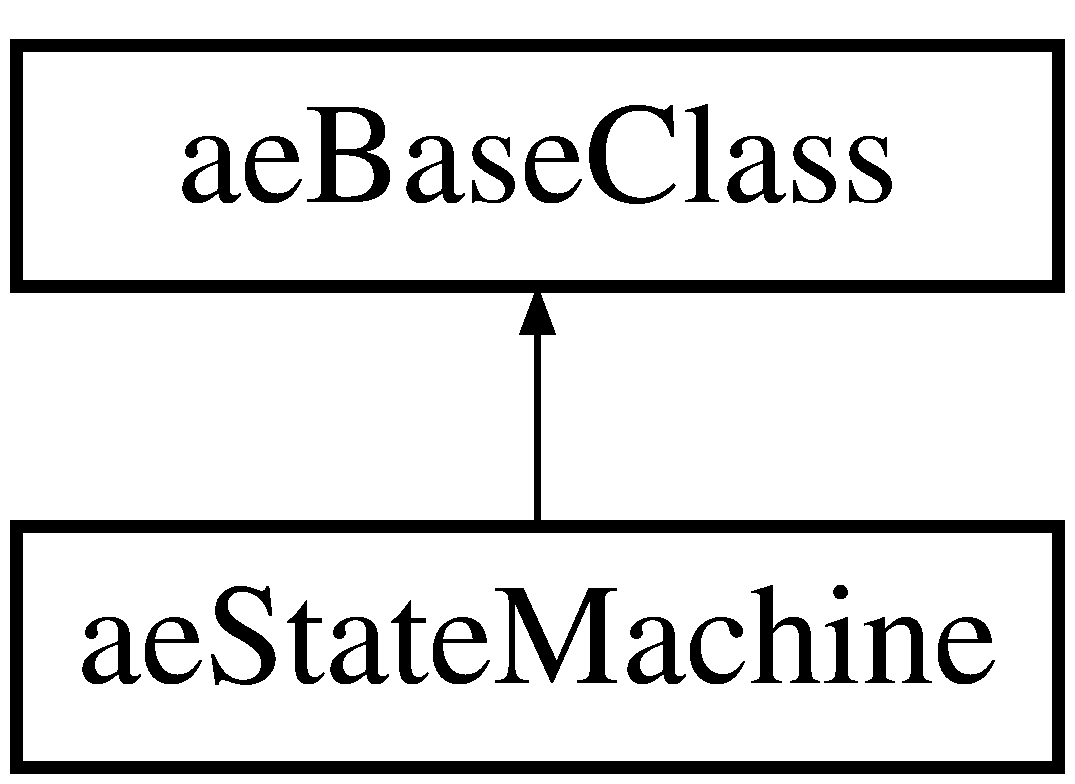
\includegraphics[height=2.000000cm]{classae_state_machine}
\end{center}
\end{figure}
\subsection*{Public Member Functions}
\begin{DoxyCompactItemize}
\item 
virtual void {\bfseries Init} (\hyperlink{classae_state_machine_script}{ae\+State\+Machine\+Script} $\ast$p\+Script)\hypertarget{classae_state_machine_a393baf6d774bed96d654f77519e6ea42}{}\label{classae_state_machine_a393baf6d774bed96d654f77519e6ea42}

\item 
virtual void {\bfseries Add\+State} (\hyperlink{class_c_state}{C\+State} $\ast$p\+New\+State)\hypertarget{classae_state_machine_a23472ec05602878dd72b525c8b887b83}{}\label{classae_state_machine_a23472ec05602878dd72b525c8b887b83}

\item 
virtual void {\bfseries Set\+State} (int New\+State)\hypertarget{classae_state_machine_a706d878305a519efe2dfbc5c716cca27}{}\label{classae_state_machine_a706d878305a519efe2dfbc5c716cca27}

\item 
virtual void {\bfseries On\+Update} (float f\+Delta, \hyperlink{classae_base_class}{ae\+Base\+Class} $\ast$p\+Object)\hypertarget{classae_state_machine_ac19ecb58275459952c74d377fab91165}{}\label{classae_state_machine_ac19ecb58275459952c74d377fab91165}

\item 
virtual void \hyperlink{classae_state_machine_a562dd6e8de039e4e18c668ee56f0b4b1}{Destroy} ()\hypertarget{classae_state_machine_a562dd6e8de039e4e18c668ee56f0b4b1}{}\label{classae_state_machine_a562dd6e8de039e4e18c668ee56f0b4b1}

\begin{DoxyCompactList}\small\item\em Destroys this object. \end{DoxyCompactList}\end{DoxyCompactItemize}
\subsection*{Protected Attributes}
\begin{DoxyCompactItemize}
\item 
\hyperlink{class_c_state}{C\+State} $\ast$ {\bfseries m\+\_\+p\+Current\+State}\hypertarget{classae_state_machine_ac489d362038343fe9cbe1bf2a97df8d8}{}\label{classae_state_machine_ac489d362038343fe9cbe1bf2a97df8d8}

\item 
\hyperlink{classae_state_machine_script}{ae\+State\+Machine\+Script} $\ast$ {\bfseries m\+\_\+p\+Script}\hypertarget{classae_state_machine_ab9ca9e9ed387fd0c0913b206f63ad902}{}\label{classae_state_machine_ab9ca9e9ed387fd0c0913b206f63ad902}

\item 
std\+::vector$<$ \hyperlink{class_c_state}{C\+State} $\ast$ $>$ {\bfseries m\+\_\+a\+Posible\+States}\hypertarget{classae_state_machine_a465820778fecdcfd694ae12d57ab5271}{}\label{classae_state_machine_a465820778fecdcfd694ae12d57ab5271}

\end{DoxyCompactItemize}


The documentation for this class was generated from the following files\+:\begin{DoxyCompactItemize}
\item 
C\+:/\+Users/\+Alvaro Estrada/\+Documents/\+Visual Studio 2015/\+Projects/\+R\+T\+S\+\_\+\+A\+E/\+R\+T\+S\+\_\+\+A\+E/\+Game/State\+Machine.\+h\item 
C\+:/\+Users/\+Alvaro Estrada/\+Documents/\+Visual Studio 2015/\+Projects/\+R\+T\+S\+\_\+\+A\+E/\+R\+T\+S\+\_\+\+A\+E/\+Game/State\+Machine.\+cpp\end{DoxyCompactItemize}

\hypertarget{classae_state_machine_script}{}\section{ae\+State\+Machine\+Script Class Reference}
\label{classae_state_machine_script}\index{ae\+State\+Machine\+Script@{ae\+State\+Machine\+Script}}
Inheritance diagram for ae\+State\+Machine\+Script\+:\begin{figure}[H]
\begin{center}
\leavevmode
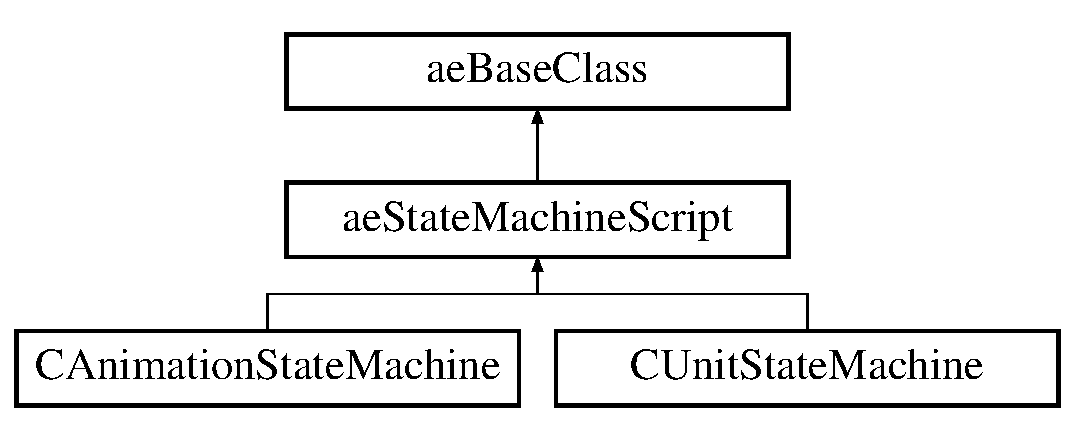
\includegraphics[height=3.000000cm]{classae_state_machine_script}
\end{center}
\end{figure}
\subsection*{Public Member Functions}
\begin{DoxyCompactItemize}
\item 
void \hyperlink{classae_state_machine_script_a6942f6b0d8ddad638e324a9fb0f9bf18}{Destroy} ()\hypertarget{classae_state_machine_script_a6942f6b0d8ddad638e324a9fb0f9bf18}{}\label{classae_state_machine_script_a6942f6b0d8ddad638e324a9fb0f9bf18}

\begin{DoxyCompactList}\small\item\em Destroys this object. \end{DoxyCompactList}\item 
virtual void {\bfseries Set\+State} (int New\+State)=0\hypertarget{classae_state_machine_script_a3b23cbf9c1fd223aedc3a749e364fd67}{}\label{classae_state_machine_script_a3b23cbf9c1fd223aedc3a749e364fd67}

\item 
void {\bfseries Set\+State\+List} (std\+::vector$<$ \hyperlink{class_c_state}{C\+State} $\ast$ $>$ $\ast$p\+State\+List)\hypertarget{classae_state_machine_script_a9a486fa08e377069d5deac8e7b0958b5}{}\label{classae_state_machine_script_a9a486fa08e377069d5deac8e7b0958b5}

\item 
void {\bfseries Set\+State\+Reference} (\hyperlink{class_c_state}{C\+State} $\ast$$\ast$Current\+State\+Reference)\hypertarget{classae_state_machine_script_ade3da83335b88ffbd673365d2b80055e}{}\label{classae_state_machine_script_ade3da83335b88ffbd673365d2b80055e}

\end{DoxyCompactItemize}
\subsection*{Protected Attributes}
\begin{DoxyCompactItemize}
\item 
std\+::vector$<$ \hyperlink{class_c_state}{C\+State} $\ast$ $>$ $\ast$ {\bfseries m\+\_\+p\+State\+List}\hypertarget{classae_state_machine_script_aa245cd1a4f354684601861546ce8fdc2}{}\label{classae_state_machine_script_aa245cd1a4f354684601861546ce8fdc2}

\item 
\hyperlink{class_c_state}{C\+State} $\ast$$\ast$ {\bfseries m\+\_\+pp\+Current\+State}\hypertarget{classae_state_machine_script_a94da15ddbb9f68be06d4ece7027a6b60}{}\label{classae_state_machine_script_a94da15ddbb9f68be06d4ece7027a6b60}

\end{DoxyCompactItemize}


The documentation for this class was generated from the following file\+:\begin{DoxyCompactItemize}
\item 
C\+:/\+Users/\+Alvaro Estrada/\+Documents/\+Visual Studio 2015/\+Projects/\+R\+T\+S\+\_\+\+A\+E/\+R\+T\+S\+\_\+\+A\+E/\+Game/State\+Machine\+Script.\+h\end{DoxyCompactItemize}

\hypertarget{classae_tiled_map}{}\section{ae\+Tiled\+Map Class Reference}
\label{classae_tiled_map}\index{ae\+Tiled\+Map@{ae\+Tiled\+Map}}
Inheritance diagram for ae\+Tiled\+Map\+:\begin{figure}[H]
\begin{center}
\leavevmode
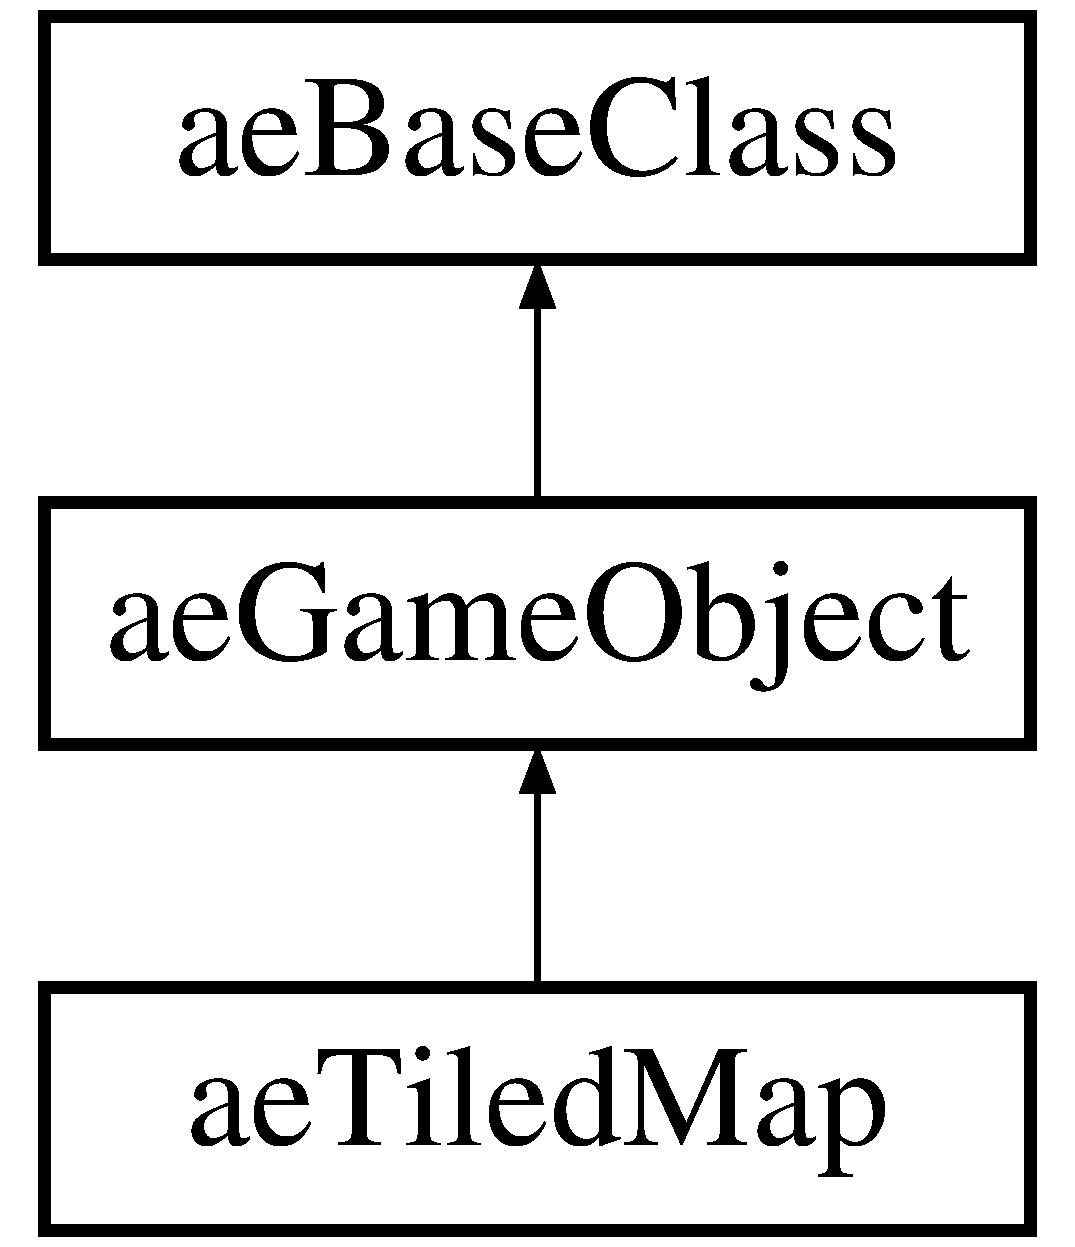
\includegraphics[height=3.000000cm]{classae_tiled_map}
\end{center}
\end{figure}
\subsection*{Classes}
\begin{DoxyCompactItemize}
\item 
class \hyperlink{classae_tiled_map_1_1ae_map_tile}{ae\+Map\+Tile}
\end{DoxyCompactItemize}
\subsection*{Public Member Functions}
\begin{DoxyCompactItemize}
\item 
int {\bfseries Init} (\hyperlink{classae_core_1_1ae_renderer}{ae\+Renderer} $\ast$p\+Renderer, Presets\+List $\ast$p\+Presets)\hypertarget{classae_tiled_map_a3e7d015f09c6cfca2a9f72f8fef9c2a4}{}\label{classae_tiled_map_a3e7d015f09c6cfca2a9f72f8fef9c2a4}

\item 
void \hyperlink{classae_tiled_map_a905504860f36560db80a307fcd3398b7}{Destroy} ()\hypertarget{classae_tiled_map_a905504860f36560db80a307fcd3398b7}{}\label{classae_tiled_map_a905504860f36560db80a307fcd3398b7}

\begin{DoxyCompactList}\small\item\em Destroys this object. \end{DoxyCompactList}\item 
void \hyperlink{classae_tiled_map_a96e6f64deda9d9d02fef3cd173e900a8}{Update} (float f\+Delta)
\begin{DoxyCompactList}\small\item\em Updates given f\+Delta. \end{DoxyCompactList}\item 
void \hyperlink{classae_tiled_map_a3f0816ebe094c6a1308524936d6c926e}{Render} (\hyperlink{classae_core_1_1ae_renderer}{ae\+Renderer} $\ast$p\+Renderer)
\begin{DoxyCompactList}\small\item\em Renders this object given its given renderer pointer. \end{DoxyCompactList}\item 
int32 {\bfseries Get\+Map\+Size} () const \hypertarget{classae_tiled_map_afcb55146c076d64a9b2f21f07fbebea4}{}\label{classae_tiled_map_afcb55146c076d64a9b2f21f07fbebea4}

\item 
\hyperlink{namespaceae_core_ad0f2d0ae721a7f0afb159366dcc2da9c}{int16} {\bfseries Get\+Cost} (const \hyperlink{namespaceae_core_a862bc39eb87cfabca273f49e2a920129}{int32} x, const \hyperlink{namespaceae_core_a862bc39eb87cfabca273f49e2a920129}{int32} y) const \hypertarget{classae_tiled_map_a9bc8dfe7b53c912d85d108bcbc303e32}{}\label{classae_tiled_map_a9bc8dfe7b53c912d85d108bcbc303e32}

\item 
void {\bfseries Set\+Cost} (const \hyperlink{namespaceae_core_a862bc39eb87cfabca273f49e2a920129}{int32} x, const \hyperlink{namespaceae_core_a862bc39eb87cfabca273f49e2a920129}{int32} y, const \hyperlink{namespaceae_core_ad0f2d0ae721a7f0afb159366dcc2da9c}{int16} Cost)\hypertarget{classae_tiled_map_a976e05f55d5f65ec74b052926aac2e52}{}\label{classae_tiled_map_a976e05f55d5f65ec74b052926aac2e52}

\item 
\hyperlink{namespaceae_core_aa13093dc911869e5b24942552898f01f}{uint8} {\bfseries Get\+Layer1} (const \hyperlink{namespaceae_core_a862bc39eb87cfabca273f49e2a920129}{int32} x, const int y) const \hypertarget{classae_tiled_map_ac670a8ca6fc5a14e2f8d45a1ffef14a2}{}\label{classae_tiled_map_ac670a8ca6fc5a14e2f8d45a1ffef14a2}

\item 
void {\bfseries Set\+Layer1} (const \hyperlink{namespaceae_core_a862bc39eb87cfabca273f49e2a920129}{int32} x, const \hyperlink{namespaceae_core_a862bc39eb87cfabca273f49e2a920129}{int32} y, const \hyperlink{namespaceae_core_aa13093dc911869e5b24942552898f01f}{uint8} Layer1\+ID)\hypertarget{classae_tiled_map_afb62dba53150e670788065f472081d13}{}\label{classae_tiled_map_afb62dba53150e670788065f472081d13}

\item 
\hyperlink{namespaceae_core_aa13093dc911869e5b24942552898f01f}{uint8} {\bfseries Get\+Layer2} (const \hyperlink{namespaceae_core_a862bc39eb87cfabca273f49e2a920129}{int32} x, const int y) const \hypertarget{classae_tiled_map_acc9f05b12b8a2e570b184c87a58bdc10}{}\label{classae_tiled_map_acc9f05b12b8a2e570b184c87a58bdc10}

\item 
void {\bfseries Set\+Layer2} (const \hyperlink{namespaceae_core_a862bc39eb87cfabca273f49e2a920129}{int32} x, const \hyperlink{namespaceae_core_a862bc39eb87cfabca273f49e2a920129}{int32} y, const \hyperlink{namespaceae_core_aa13093dc911869e5b24942552898f01f}{uint8} Layer2\+ID)\hypertarget{classae_tiled_map_a1f7cfb290930d7b3df0c38f353ba9fdc}{}\label{classae_tiled_map_a1f7cfb290930d7b3df0c38f353ba9fdc}

\item 
\hyperlink{namespaceae_core_aa13093dc911869e5b24942552898f01f}{uint8} {\bfseries Get\+Layer3} (const \hyperlink{namespaceae_core_a862bc39eb87cfabca273f49e2a920129}{int32} x, const int y) const \hypertarget{classae_tiled_map_a70e7122adc6c87b5017f3ff4af4b37f6}{}\label{classae_tiled_map_a70e7122adc6c87b5017f3ff4af4b37f6}

\item 
void {\bfseries Set\+Layer3} (const \hyperlink{namespaceae_core_a862bc39eb87cfabca273f49e2a920129}{int32} x, const \hyperlink{namespaceae_core_a862bc39eb87cfabca273f49e2a920129}{int32} y, const \hyperlink{namespaceae_core_aa13093dc911869e5b24942552898f01f}{uint8} Layer3\+ID)\hypertarget{classae_tiled_map_a2e398db234d564da4c23ca788a4b9213}{}\label{classae_tiled_map_a2e398db234d564da4c23ca788a4b9213}

\item 
\hyperlink{namespaceae_core_aa13093dc911869e5b24942552898f01f}{uint8} {\bfseries Get\+Layer4} (const \hyperlink{namespaceae_core_a862bc39eb87cfabca273f49e2a920129}{int32} x, const int y) const \hypertarget{classae_tiled_map_a167fd038a487acb3a3399655aaa9166d}{}\label{classae_tiled_map_a167fd038a487acb3a3399655aaa9166d}

\item 
void {\bfseries Set\+Layer4} (const \hyperlink{namespaceae_core_a862bc39eb87cfabca273f49e2a920129}{int32} x, const \hyperlink{namespaceae_core_a862bc39eb87cfabca273f49e2a920129}{int32} y, const \hyperlink{namespaceae_core_aa13093dc911869e5b24942552898f01f}{uint8} Layer4\+ID)\hypertarget{classae_tiled_map_aadf5b09bfa3e89af39365953a3bdc2d3}{}\label{classae_tiled_map_aadf5b09bfa3e89af39365953a3bdc2d3}

\item 
\hyperlink{namespaceae_core_aa13093dc911869e5b24942552898f01f}{uint8} {\bfseries Get\+Layer5} (const \hyperlink{namespaceae_core_a862bc39eb87cfabca273f49e2a920129}{int32} x, const int y) const \hypertarget{classae_tiled_map_aee47578443d133aa85c47faa029338e1}{}\label{classae_tiled_map_aee47578443d133aa85c47faa029338e1}

\item 
void {\bfseries Set\+Layer5} (const \hyperlink{namespaceae_core_a862bc39eb87cfabca273f49e2a920129}{int32} x, const \hyperlink{namespaceae_core_a862bc39eb87cfabca273f49e2a920129}{int32} y, const \hyperlink{namespaceae_core_aa13093dc911869e5b24942552898f01f}{uint8} Layer5\+ID)\hypertarget{classae_tiled_map_a98a3fb8227506b4374b411fd258d0e4e}{}\label{classae_tiled_map_a98a3fb8227506b4374b411fd258d0e4e}

\item 
float {\bfseries Get\+Influence} (const \hyperlink{namespaceae_core_a862bc39eb87cfabca273f49e2a920129}{int32} x, const int y) const \hypertarget{classae_tiled_map_a40b31b58e772fc57ded4a397197cd550}{}\label{classae_tiled_map_a40b31b58e772fc57ded4a397197cd550}

\item 
void {\bfseries Set\+Influence} (const \hyperlink{namespaceae_core_a862bc39eb87cfabca273f49e2a920129}{int32} x, const \hyperlink{namespaceae_core_a862bc39eb87cfabca273f49e2a920129}{int32} y, const float Influence)\hypertarget{classae_tiled_map_aaaec14e8d52ceac9a69eb0d0db4ea940}{}\label{classae_tiled_map_aaaec14e8d52ceac9a69eb0d0db4ea940}

\item 
void {\bfseries Show\+Grid} (bool \hyperlink{_base_class_8h_aded8224779c70fab5084220935d672bba46a2a41cc6e552044816a2d04634545d}{State})\hypertarget{classae_tiled_map_a258662b085cfddb882576c85effbfca9}{}\label{classae_tiled_map_a258662b085cfddb882576c85effbfca9}

\item 
void {\bfseries Set\+View} (bool Isometric)\hypertarget{classae_tiled_map_a3cde4546fc42a71eb713c39a1a98ea09}{}\label{classae_tiled_map_a3cde4546fc42a71eb713c39a1a98ea09}

\item 
void {\bfseries Set\+Path\+Finder} (int Path\+Finder)\hypertarget{classae_tiled_map_ae724a523cc32ad46822b51cc62a3b0e6}{}\label{classae_tiled_map_ae724a523cc32ad46822b51cc62a3b0e6}

\item 
void {\bfseries Camera\+Reference} (\hyperlink{classae_world}{ae\+World} $\ast$Camera)\hypertarget{classae_tiled_map_aa0db9965530414129013d0c698a2b13d}{}\label{classae_tiled_map_aa0db9965530414129013d0c698a2b13d}

\item 
void {\bfseries Update\+Render\+Texture} (\hyperlink{classae_core_1_1ae_renderer}{ae\+Renderer} $\ast$p\+Renderer)\hypertarget{classae_tiled_map_a510e48b848df51bfcd3ea69d8bb5dab7}{}\label{classae_tiled_map_a510e48b848df51bfcd3ea69d8bb5dab7}

\item 
void {\bfseries Make\+Search} (\hyperlink{structae_core_1_1ae_point}{ae\+Point} Start\+Position, \hyperlink{structae_core_1_1ae_point}{ae\+Point} End\+Position)\hypertarget{classae_tiled_map_a5122122f68b1557224db6cc616bccd12}{}\label{classae_tiled_map_a5122122f68b1557224db6cc616bccd12}

\end{DoxyCompactItemize}
\subsection*{Static Public Member Functions}
\begin{DoxyCompactItemize}
\item 
static int {\bfseries Tile\+Map\+Creation} (void $\ast$data, int argument\+\_\+count, char $\ast$$\ast$argument\+\_\+values, char $\ast$$\ast$psz\+Col\+Name)\hypertarget{classae_tiled_map_aad3cfb01a53a5665f3d896ff336efcb8}{}\label{classae_tiled_map_aad3cfb01a53a5665f3d896ff336efcb8}

\item 
static int {\bfseries Influence\+Definition} (void $\ast$data, int argument\+\_\+count, char $\ast$$\ast$argument\+\_\+values, char $\ast$$\ast$psz\+Col\+Name)\hypertarget{classae_tiled_map_af68963b8610289c1182c572d2c544737}{}\label{classae_tiled_map_af68963b8610289c1182c572d2c544737}

\end{DoxyCompactItemize}
\subsection*{Public Attributes}
\begin{DoxyCompactItemize}
\item 
int {\bfseries Position\+Of\+Open\+Mask}\hypertarget{classae_tiled_map_a8dbef291dc8e226f273e07883d590c6a}{}\label{classae_tiled_map_a8dbef291dc8e226f273e07883d590c6a}

\item 
int {\bfseries Position\+Of\+Visited\+Mask}\hypertarget{classae_tiled_map_a793cdb801de57b17a9cdc24ccf976b0a}{}\label{classae_tiled_map_a793cdb801de57b17a9cdc24ccf976b0a}

\item 
int {\bfseries Position\+Of\+Influence\+Mask}\hypertarget{classae_tiled_map_ae586f5557fe67623df0f8994035d6dfd}{}\label{classae_tiled_map_ae586f5557fe67623df0f8994035d6dfd}

\end{DoxyCompactItemize}
\subsection*{Protected Attributes}
\begin{DoxyCompactItemize}
\item 
\hyperlink{classae_tiled_map_1_1ae_map_tile}{ae\+Map\+Tile} $\ast$$\ast$ \hyperlink{classae_tiled_map_aacd425ffb4f463b3617337355aab2aba}{m\+\_\+pp\+Map\+Grid}\hypertarget{classae_tiled_map_aacd425ffb4f463b3617337355aab2aba}{}\label{classae_tiled_map_aacd425ffb4f463b3617337355aab2aba}

\begin{DoxyCompactList}\small\item\em Map information. \end{DoxyCompactList}\item 
int32 \hyperlink{classae_tiled_map_a5b729d615199651de4a16b80bca21581}{m\+\_\+n\+Map\+Size}\hypertarget{classae_tiled_map_a5b729d615199651de4a16b80bca21581}{}\label{classae_tiled_map_a5b729d615199651de4a16b80bca21581}

\begin{DoxyCompactList}\small\item\em Map Size. \end{DoxyCompactList}\item 
int32 \hyperlink{classae_tiled_map_a7b63c3c1824027d372e9b5b626e68163}{m\+\_\+n\+Tile\+SizeX}\hypertarget{classae_tiled_map_a7b63c3c1824027d372e9b5b626e68163}{}\label{classae_tiled_map_a7b63c3c1824027d372e9b5b626e68163}

\begin{DoxyCompactList}\small\item\em The tile size in x. \end{DoxyCompactList}\item 
int32 \hyperlink{classae_tiled_map_a419ddab268eb19a325969277aa152471}{m\+\_\+n\+Tile\+SizeY}\hypertarget{classae_tiled_map_a419ddab268eb19a325969277aa152471}{}\label{classae_tiled_map_a419ddab268eb19a325969277aa152471}

\begin{DoxyCompactList}\small\item\em The tile size in y. \end{DoxyCompactList}\item 
ae\+Point {\bfseries m\+\_\+\+Precalc\+Size}\hypertarget{classae_tiled_map_aa486053be2f9ac90fe3ddd819c93361a}{}\label{classae_tiled_map_aa486053be2f9ac90fe3ddd819c93361a}

\item 
\hyperlink{classae_world}{ae\+World} $\ast$ \hyperlink{classae_tiled_map_a5ca0d7e7e07f9af20a03844b2838fd9d}{m\+\_\+p\+Camera}\hypertarget{classae_tiled_map_a5ca0d7e7e07f9af20a03844b2838fd9d}{}\label{classae_tiled_map_a5ca0d7e7e07f9af20a03844b2838fd9d}

\begin{DoxyCompactList}\small\item\em The camera. \end{DoxyCompactList}\item 
std\+::vector$<$ \hyperlink{classae_tile_type}{ae\+Tile\+Type} $\ast$ $>$ \hyperlink{classae_tiled_map_a09b498b021eb6ccdec0296355217b665}{m\+\_\+p\+Tile\+Types}\hypertarget{classae_tiled_map_a09b498b021eb6ccdec0296355217b665}{}\label{classae_tiled_map_a09b498b021eb6ccdec0296355217b665}

\begin{DoxyCompactList}\small\item\em The presets for tile creation. \end{DoxyCompactList}\item 
bool \hyperlink{classae_tiled_map_a88b87b8bc89f5768032ca6e33a82774a}{m\+\_\+b\+Show\+Grid}\hypertarget{classae_tiled_map_a88b87b8bc89f5768032ca6e33a82774a}{}\label{classae_tiled_map_a88b87b8bc89f5768032ca6e33a82774a}

\begin{DoxyCompactList}\small\item\em Flag to indicate if the grid will be shown or not. \end{DoxyCompactList}\item 
bool \hyperlink{classae_tiled_map_a705451931bd414b0d9b3d87164eae0fc}{m\+\_\+b\+Isometric}\hypertarget{classae_tiled_map_a705451931bd414b0d9b3d87164eae0fc}{}\label{classae_tiled_map_a705451931bd414b0d9b3d87164eae0fc}

\begin{DoxyCompactList}\small\item\em Flag to indicate if is isometric or not. \end{DoxyCompactList}\item 
bool {\bfseries m\+\_\+b\+Debug}\hypertarget{classae_tiled_map_a5eaca4b67487ab17c25d75527ed5e339}{}\label{classae_tiled_map_a5eaca4b67487ab17c25d75527ed5e339}

\item 
int {\bfseries m\+\_\+n\+Path\+Finder}\hypertarget{classae_tiled_map_ad47799807fc006d5ece12a1c2dbed7d8}{}\label{classae_tiled_map_ad47799807fc006d5ece12a1c2dbed7d8}

\end{DoxyCompactItemize}


\subsection{Member Function Documentation}
\index{ae\+Tiled\+Map@{ae\+Tiled\+Map}!Render@{Render}}
\index{Render@{Render}!ae\+Tiled\+Map@{ae\+Tiled\+Map}}
\subsubsection[{\texorpdfstring{Render(ae\+Renderer $\ast$p\+Renderer)}{Render(aeRenderer *pRenderer)}}]{\setlength{\rightskip}{0pt plus 5cm}void ae\+Tiled\+Map\+::\+Render (
\begin{DoxyParamCaption}
\item[{{\bf ae\+Renderer} $\ast$}]{p\+Renderer}
\end{DoxyParamCaption}
)\hspace{0.3cm}{\ttfamily [virtual]}}\hypertarget{classae_tiled_map_a3f0816ebe094c6a1308524936d6c926e}{}\label{classae_tiled_map_a3f0816ebe094c6a1308524936d6c926e}


Renders this object given its given renderer pointer. 


\begin{DoxyParams}[1]{Parameters}
\mbox{\tt in,out}  & {\em p\+Renderer} & If non-\/null, the renderer. \\
\hline
\end{DoxyParams}


Reimplemented from \hyperlink{classae_game_object_ae2ab1d6a65f6008766faa8295affc9fe}{ae\+Game\+Object}.

\index{ae\+Tiled\+Map@{ae\+Tiled\+Map}!Update@{Update}}
\index{Update@{Update}!ae\+Tiled\+Map@{ae\+Tiled\+Map}}
\subsubsection[{\texorpdfstring{Update(float f\+Delta)}{Update(float fDelta)}}]{\setlength{\rightskip}{0pt plus 5cm}void ae\+Tiled\+Map\+::\+Update (
\begin{DoxyParamCaption}
\item[{float}]{f\+Delta}
\end{DoxyParamCaption}
)\hspace{0.3cm}{\ttfamily [virtual]}}\hypertarget{classae_tiled_map_a96e6f64deda9d9d02fef3cd173e900a8}{}\label{classae_tiled_map_a96e6f64deda9d9d02fef3cd173e900a8}


Updates given f\+Delta. 


\begin{DoxyParams}{Parameters}
{\em f\+Delta} & The delta. \\
\hline
\end{DoxyParams}


Reimplemented from \hyperlink{classae_game_object_ab43b31f1179579df835873e60ae84f32}{ae\+Game\+Object}.



The documentation for this class was generated from the following files\+:\begin{DoxyCompactItemize}
\item 
C\+:/\+Users/\+Alvaro Estrada/\+Documents/\+Visual Studio 2015/\+Projects/\+R\+T\+S\+\_\+\+A\+E/\+R\+T\+S\+\_\+\+A\+E/\+Game/Tiled\+Map.\+h\item 
C\+:/\+Users/\+Alvaro Estrada/\+Documents/\+Visual Studio 2015/\+Projects/\+R\+T\+S\+\_\+\+A\+E/\+R\+T\+S\+\_\+\+A\+E/\+Game/Tiled\+Map.\+cpp\end{DoxyCompactItemize}

\hypertarget{classae_tile_type}{}\section{ae\+Tile\+Type Class Reference}
\label{classae_tile_type}\index{ae\+Tile\+Type@{ae\+Tile\+Type}}
Inheritance diagram for ae\+Tile\+Type\+:\begin{figure}[H]
\begin{center}
\leavevmode
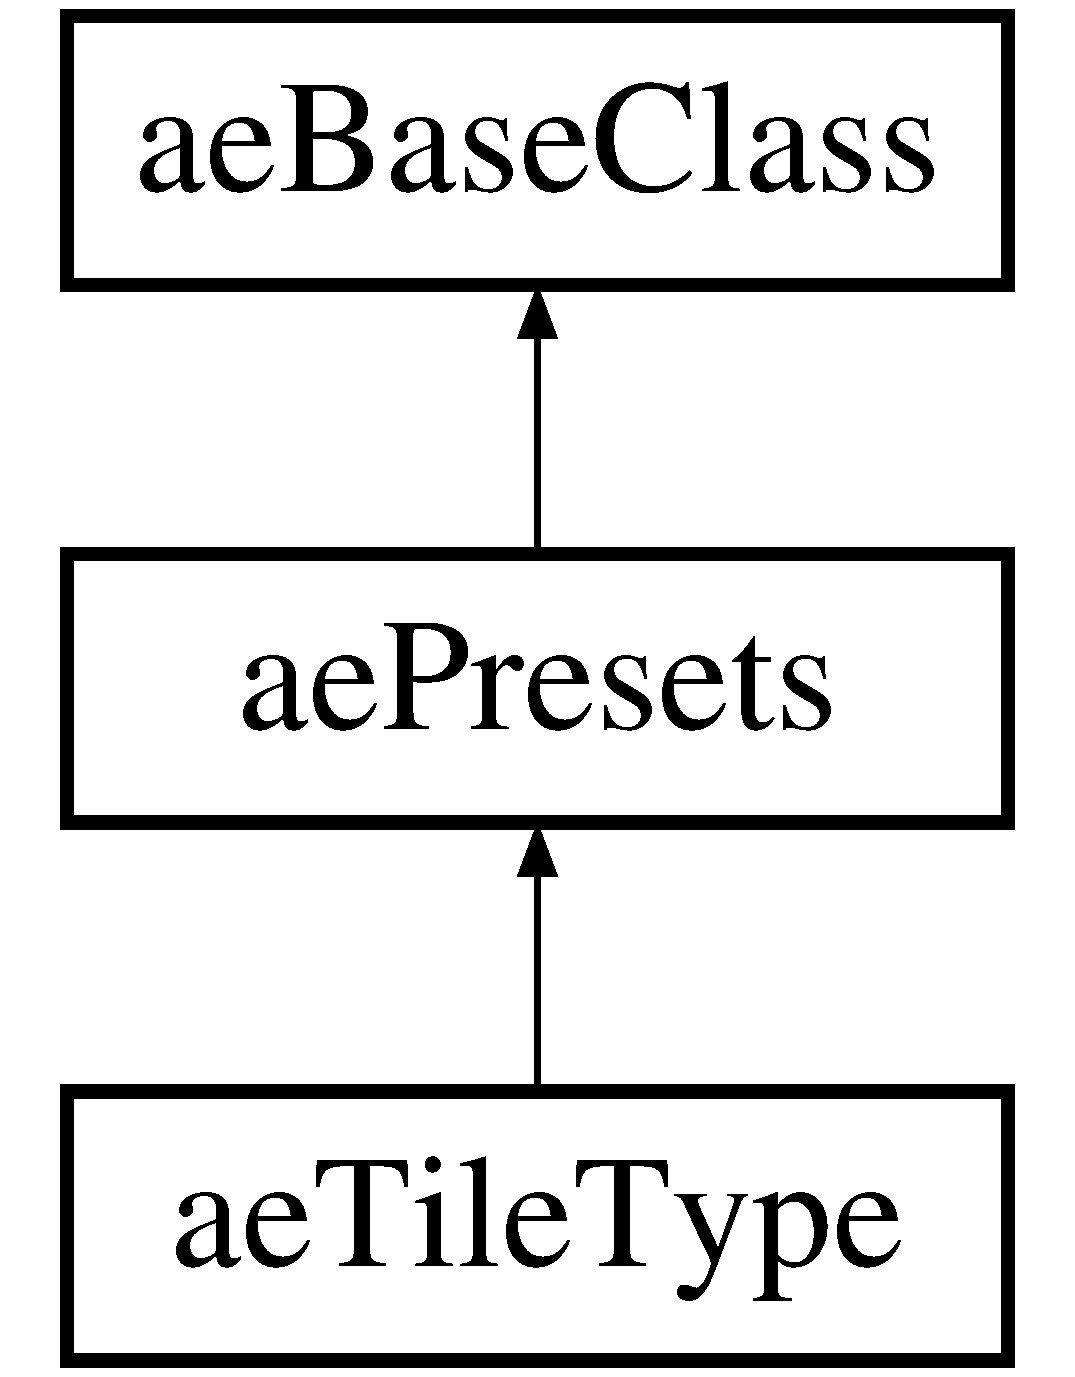
\includegraphics[height=3.000000cm]{classae_tile_type}
\end{center}
\end{figure}
\subsection*{Public Member Functions}
\begin{DoxyCompactItemize}
\item 
{\bfseries ae\+Tile\+Type} (int ID, ae\+String Name, int Cost, ae\+Sprite $\ast$Tile\+Image, int Sprite\+ID, bool Isometric, int Movement)\hypertarget{classae_tile_type_ad606d9235b08645c3f196edb23c6125c}{}\label{classae_tile_type_ad606d9235b08645c3f196edb23c6125c}

\end{DoxyCompactItemize}
\subsection*{Public Attributes}
\begin{DoxyCompactItemize}
\item 
int {\bfseries m\+\_\+n\+ID}\hypertarget{classae_tile_type_acfaf4ff6be3b428fd6874bc243900564}{}\label{classae_tile_type_acfaf4ff6be3b428fd6874bc243900564}

\item 
ae\+String {\bfseries m\+\_\+psz\+Name}\hypertarget{classae_tile_type_a11c7de6ca5c8d9f85f47157b3a8dad5c}{}\label{classae_tile_type_a11c7de6ca5c8d9f85f47157b3a8dad5c}

\item 
int {\bfseries m\+\_\+n\+Cost}\hypertarget{classae_tile_type_abd0818de5b6b1671d80b03b22f2954fe}{}\label{classae_tile_type_abd0818de5b6b1671d80b03b22f2954fe}

\item 
ae\+Sprite $\ast$ {\bfseries m\+\_\+p\+Image}\hypertarget{classae_tile_type_a77d769c4f2cf197eeabc0171d97a4788}{}\label{classae_tile_type_a77d769c4f2cf197eeabc0171d97a4788}

\item 
int {\bfseries m\+\_\+n\+Sprite\+ID}\hypertarget{classae_tile_type_a1cd89c50b538253f21d33d857aede022}{}\label{classae_tile_type_a1cd89c50b538253f21d33d857aede022}

\item 
bool {\bfseries m\+\_\+b\+Isometric}\hypertarget{classae_tile_type_ac2123be395c87bb58d44ab7109e28738}{}\label{classae_tile_type_ac2123be395c87bb58d44ab7109e28738}

\item 
int {\bfseries m\+\_\+n\+Movement}\hypertarget{classae_tile_type_a43b3dc7d3edd3cbcfba71f9a89cc3896}{}\label{classae_tile_type_a43b3dc7d3edd3cbcfba71f9a89cc3896}

\end{DoxyCompactItemize}
\subsection*{Additional Inherited Members}


The documentation for this class was generated from the following files\+:\begin{DoxyCompactItemize}
\item 
C\+:/\+Users/\+Alvaro Estrada/\+Documents/\+Visual Studio 2015/\+Projects/\+R\+T\+S\+\_\+\+A\+E/\+R\+T\+S\+\_\+\+A\+E/\+Game/Tile\+Type.\+h\item 
C\+:/\+Users/\+Alvaro Estrada/\+Documents/\+Visual Studio 2015/\+Projects/\+R\+T\+S\+\_\+\+A\+E/\+R\+T\+S\+\_\+\+A\+E/\+Game/Tile\+Type.\+cpp\end{DoxyCompactItemize}

\hypertarget{structae_transform}{}\section{ae\+Transform Struct Reference}
\label{structae_transform}\index{ae\+Transform@{ae\+Transform}}


Is a storage for the necessary components for a Game\+Object physics.  




{\ttfamily \#include $<$Transform.\+h$>$}

\subsection*{Public Attributes}
\begin{DoxyCompactItemize}
\item 
\hyperlink{structae_core_1_1ae_vector3}{ae\+Core\+::ae\+Vector3} {\bfseries Position}\hypertarget{structae_transform_a8c34eee85f9fd54dad0e5c2c87cd82ff}{}\label{structae_transform_a8c34eee85f9fd54dad0e5c2c87cd82ff}

\item 
\hyperlink{structae_core_1_1ae_vector3}{ae\+Core\+::ae\+Vector3} {\bfseries Velocity}\hypertarget{structae_transform_acebbcda61af0dc18894b1ffb7845ac1b}{}\label{structae_transform_acebbcda61af0dc18894b1ffb7845ac1b}

\item 
\hyperlink{structae_core_1_1ae_vector3}{ae\+Core\+::ae\+Vector3} {\bfseries Direction}\hypertarget{structae_transform_adecd5e97a7612957cf5f707b55802c97}{}\label{structae_transform_adecd5e97a7612957cf5f707b55802c97}

\item 
\hyperlink{structae_core_1_1ae_vector3}{ae\+Core\+::ae\+Vector3} {\bfseries Scale}\hypertarget{structae_transform_ac50ef3c1832ed4fbb4601192069f1ba7}{}\label{structae_transform_ac50ef3c1832ed4fbb4601192069f1ba7}

\end{DoxyCompactItemize}


\subsection{Detailed Description}
Is a storage for the necessary components for a Game\+Object physics. 

The documentation for this struct was generated from the following files\+:\begin{DoxyCompactItemize}
\item 
C\+:/\+Users/\+Alvaro Estrada/\+Documents/\+Visual Studio 2015/\+Projects/\+R\+T\+S\+\_\+\+A\+E/\+R\+T\+S\+\_\+\+A\+E/\+Game/\hyperlink{_transform_8h}{Transform.\+h}\item 
C\+:/\+Users/\+Alvaro Estrada/\+Documents/\+Visual Studio 2015/\+Projects/\+R\+T\+S\+\_\+\+A\+E/\+R\+T\+S\+\_\+\+A\+E/\+Game/Transform.\+cpp\end{DoxyCompactItemize}

\hypertarget{classae_unit_type}{}\section{ae\+Unit\+Type Class Reference}
\label{classae_unit_type}\index{ae\+Unit\+Type@{ae\+Unit\+Type}}


A unit type.  




{\ttfamily \#include $<$Unit\+Type.\+h$>$}

Inheritance diagram for ae\+Unit\+Type\+:\begin{figure}[H]
\begin{center}
\leavevmode
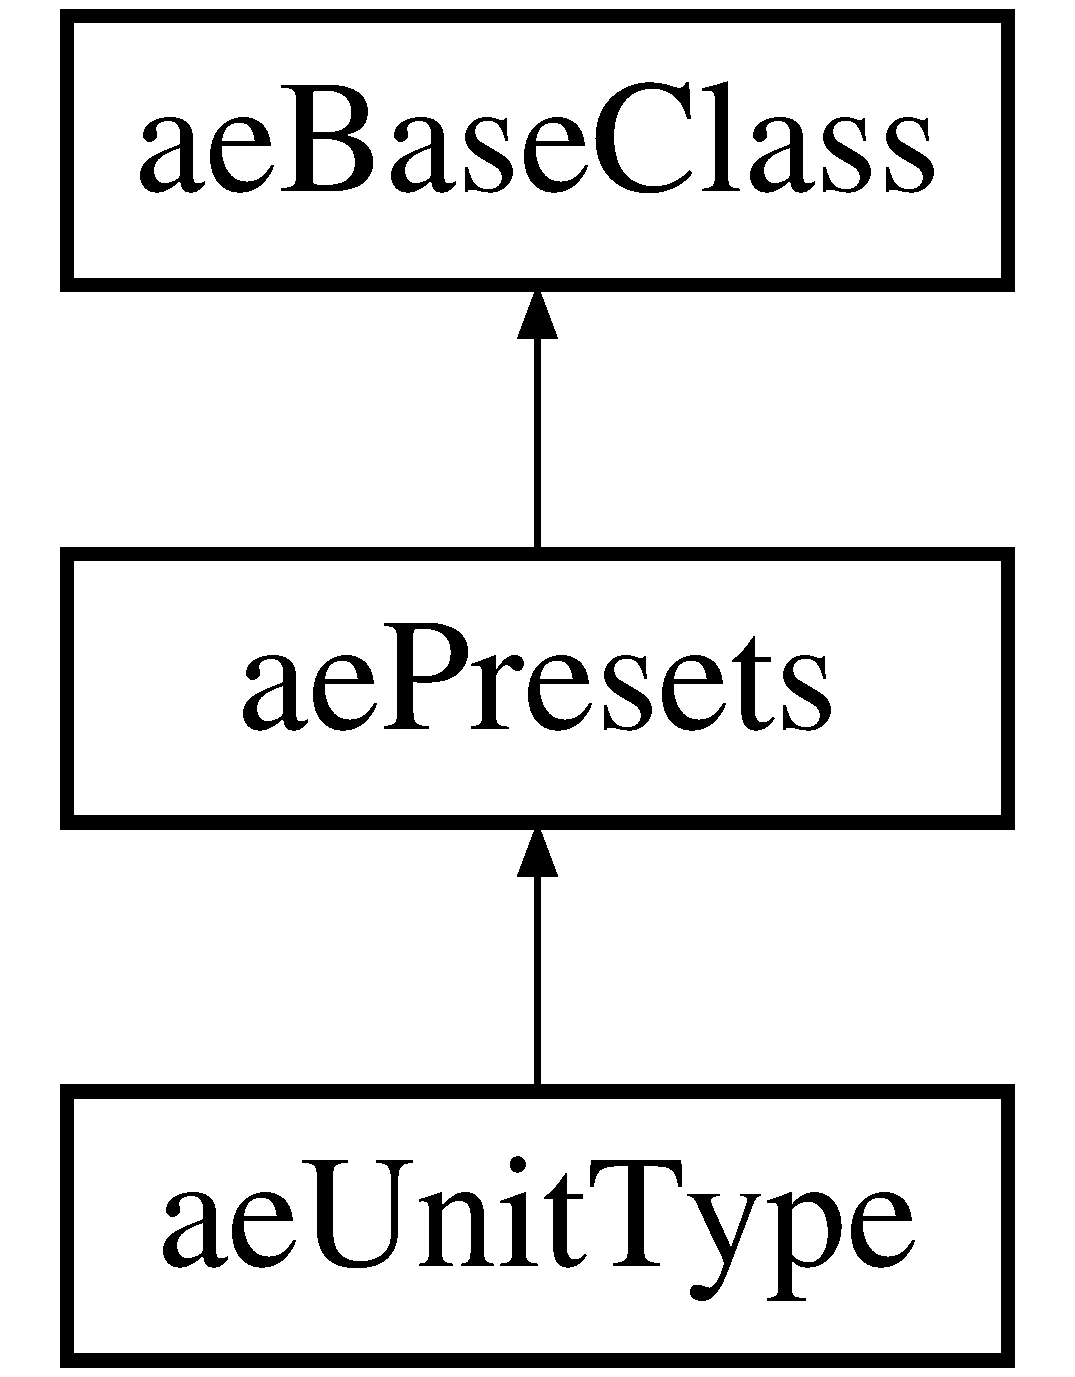
\includegraphics[height=3.000000cm]{classae_unit_type}
\end{center}
\end{figure}
\subsection*{Public Member Functions}
\begin{DoxyCompactItemize}
\item 
void \hyperlink{classae_unit_type_a3cc8f03c8c3abb2893d1adcae0692059}{Destroy} ()\hypertarget{classae_unit_type_a3cc8f03c8c3abb2893d1adcae0692059}{}\label{classae_unit_type_a3cc8f03c8c3abb2893d1adcae0692059}

\begin{DoxyCompactList}\small\item\em Destroys this object. \end{DoxyCompactList}\end{DoxyCompactItemize}
\subsection*{Public Attributes}
\begin{DoxyCompactItemize}
\item 
\begin{tabbing}
xx\=xx\=xx\=xx\=xx\=xx\=xx\=xx\=xx\=\kill
union \{\\
\>struct \{\\
\>\>bool {\bfseries IsMilitant}: 1\\
\>\>bool {\bfseries CanBuild}: 1\\
\>\} \hypertarget{unionae_unit_type_1_1_0D42_a99acaf3c4289cb6f97709bcc8f16a735}{}\label{unionae_unit_type_1_1_0D42_a99acaf3c4289cb6f97709bcc8f16a735}
\\
\>bool {\bfseries BehaviourFlags}\\
\}; \hypertarget{classae_unit_type_a0546ed04de220f2de4638774be84119d}{}\label{classae_unit_type_a0546ed04de220f2de4638774be84119d}
\\

\end{tabbing}\item 
int {\bfseries m\+\_\+n\+ID}\hypertarget{classae_unit_type_a5f86adb71d05c12f5a60f8dc3a7b37e5}{}\label{classae_unit_type_a5f86adb71d05c12f5a60f8dc3a7b37e5}

\item 
int {\bfseries m\+\_\+n\+Radius}\hypertarget{classae_unit_type_a9651b91c590e29b5d2f78771b53c2c08}{}\label{classae_unit_type_a9651b91c590e29b5d2f78771b53c2c08}

\item 
int {\bfseries m\+\_\+n\+Image\+ID}\hypertarget{classae_unit_type_a4f160385b754f3cde47d9b2dbe862457}{}\label{classae_unit_type_a4f160385b754f3cde47d9b2dbe862457}

\item 
ae\+String {\bfseries m\+\_\+psz\+Name}\hypertarget{classae_unit_type_a30066454b57ef80410de6169e6cc5ccb}{}\label{classae_unit_type_a30066454b57ef80410de6169e6cc5ccb}

\item 
float {\bfseries m\+\_\+f\+H\+P\+\_\+\+Max}\hypertarget{classae_unit_type_aca7918ed07a1484cdf3b424e0d8c279a}{}\label{classae_unit_type_aca7918ed07a1484cdf3b424e0d8c279a}

\item 
float {\bfseries m\+\_\+f\+Attack\+\_\+\+Range\+\_\+\+Max}\hypertarget{classae_unit_type_a90884afa6cd494f398e0ded9fec26dd8}{}\label{classae_unit_type_a90884afa6cd494f398e0ded9fec26dd8}

\item 
float {\bfseries m\+\_\+f\+Attack\+\_\+\+Range\+\_\+\+Min}\hypertarget{classae_unit_type_af595f0770639337dcd61876c06ac8e89}{}\label{classae_unit_type_af595f0770639337dcd61876c06ac8e89}

\item 
float {\bfseries m\+\_\+f\+Attack\+\_\+\+Speed}\hypertarget{classae_unit_type_a9e415033278b6a6e820b7397b1a2d1f0}{}\label{classae_unit_type_a9e415033278b6a6e820b7397b1a2d1f0}

\item 
float {\bfseries m\+\_\+f\+View\+\_\+\+Range}\hypertarget{classae_unit_type_aaf32bc0f8d0466c77f704f3aafe731f7}{}\label{classae_unit_type_aaf32bc0f8d0466c77f704f3aafe731f7}

\item 
float {\bfseries m\+\_\+f\+Speed}\hypertarget{classae_unit_type_af65cbed874be7bda304c9ab02c41c0bd}{}\label{classae_unit_type_af65cbed874be7bda304c9ab02c41c0bd}

\item 
float {\bfseries m\+\_\+f\+Strength}\hypertarget{classae_unit_type_ac8ea8815e995e9d7eb9ba495b3bc44e2}{}\label{classae_unit_type_ac8ea8815e995e9d7eb9ba495b3bc44e2}

\item 
void $\ast$ {\bfseries m\+\_\+p\+Image}\hypertarget{classae_unit_type_a6f886bb6dc0fc70aeb00c54db295c416}{}\label{classae_unit_type_a6f886bb6dc0fc70aeb00c54db295c416}

\end{DoxyCompactItemize}
\subsection*{Additional Inherited Members}


\subsection{Detailed Description}
A unit type. 

The documentation for this class was generated from the following files\+:\begin{DoxyCompactItemize}
\item 
C\+:/\+Users/\+Alvaro Estrada/\+Documents/\+Visual Studio 2015/\+Projects/\+R\+T\+S\+\_\+\+A\+E/\+R\+T\+S\+\_\+\+A\+E/\+Game/\hyperlink{_unit_type_8h}{Unit\+Type.\+h}\item 
C\+:/\+Users/\+Alvaro Estrada/\+Documents/\+Visual Studio 2015/\+Projects/\+R\+T\+S\+\_\+\+A\+E/\+R\+T\+S\+\_\+\+A\+E/\+Game/Unit\+Type.\+cpp\end{DoxyCompactItemize}

\hypertarget{structae_core_1_1ae_user_event}{}\section{ae\+Core\+:\+:ae\+User\+Event Struct Reference}
\label{structae_core_1_1ae_user_event}\index{ae\+Core\+::ae\+User\+Event@{ae\+Core\+::ae\+User\+Event}}


A user event.  




{\ttfamily \#include $<$Events\+System.\+h$>$}

Inheritance diagram for ae\+Core\+:\+:ae\+User\+Event\+:\begin{figure}[H]
\begin{center}
\leavevmode
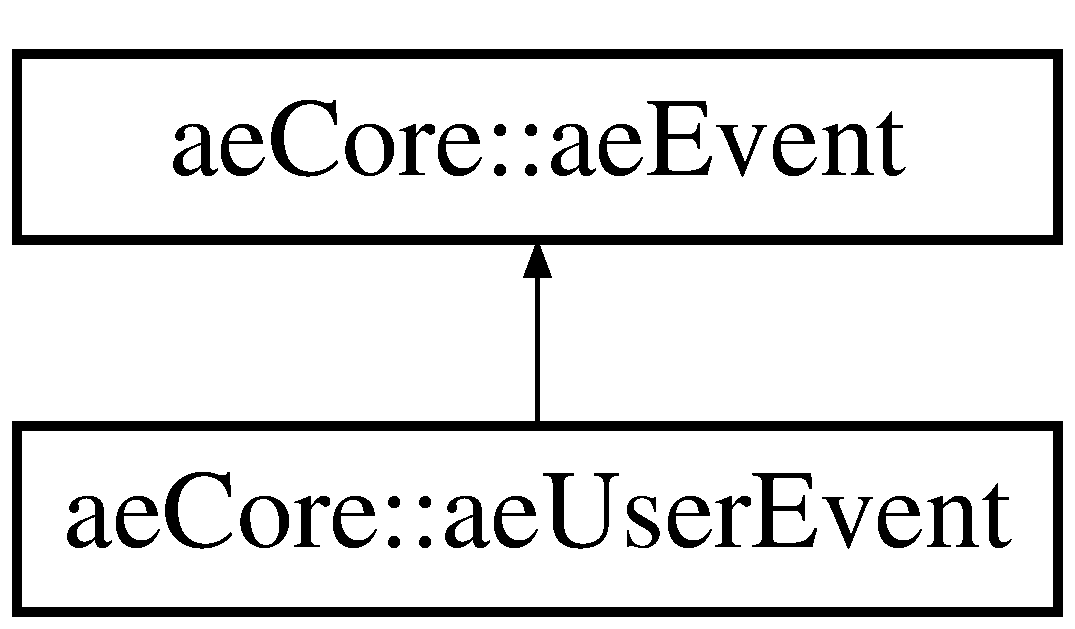
\includegraphics[height=2.000000cm]{structae_core_1_1ae_user_event}
\end{center}
\end{figure}
\subsection*{Public Attributes}
\begin{DoxyCompactItemize}
\item 
\hyperlink{namespaceae_core_aa13093dc911869e5b24942552898f01f}{uint8} {\bfseries Code}\hypertarget{structae_core_1_1ae_user_event_a4f80ce8bd55f94a07e60f7140892cf5e}{}\label{structae_core_1_1ae_user_event_a4f80ce8bd55f94a07e60f7140892cf5e}

\item 
void $\ast$ {\bfseries Data1}\hypertarget{structae_core_1_1ae_user_event_a5e4c9f121f7e9c91c291f5de7d77f5ca}{}\label{structae_core_1_1ae_user_event_a5e4c9f121f7e9c91c291f5de7d77f5ca}

\item 
void $\ast$ {\bfseries Data2}\hypertarget{structae_core_1_1ae_user_event_a60a7b8d60f77ecac995251f9fc914b54}{}\label{structae_core_1_1ae_user_event_a60a7b8d60f77ecac995251f9fc914b54}

\end{DoxyCompactItemize}


\subsection{Detailed Description}
A user event. 

The documentation for this struct was generated from the following file\+:\begin{DoxyCompactItemize}
\item 
C\+:/\+Users/\+Alvaro Estrada/\+Documents/\+Visual Studio 2015/\+Projects/\+R\+T\+S\+\_\+\+A\+E/ae\+Core/\+Event\+System/Events\+System.\+h\end{DoxyCompactItemize}

\hypertarget{classae_user_script}{}\section{ae\+User\+Script Class Reference}
\label{classae_user_script}\index{ae\+User\+Script@{ae\+User\+Script}}


An user script.  




{\ttfamily \#include $<$User\+Script.\+h$>$}

Inheritance diagram for ae\+User\+Script\+:\begin{figure}[H]
\begin{center}
\leavevmode
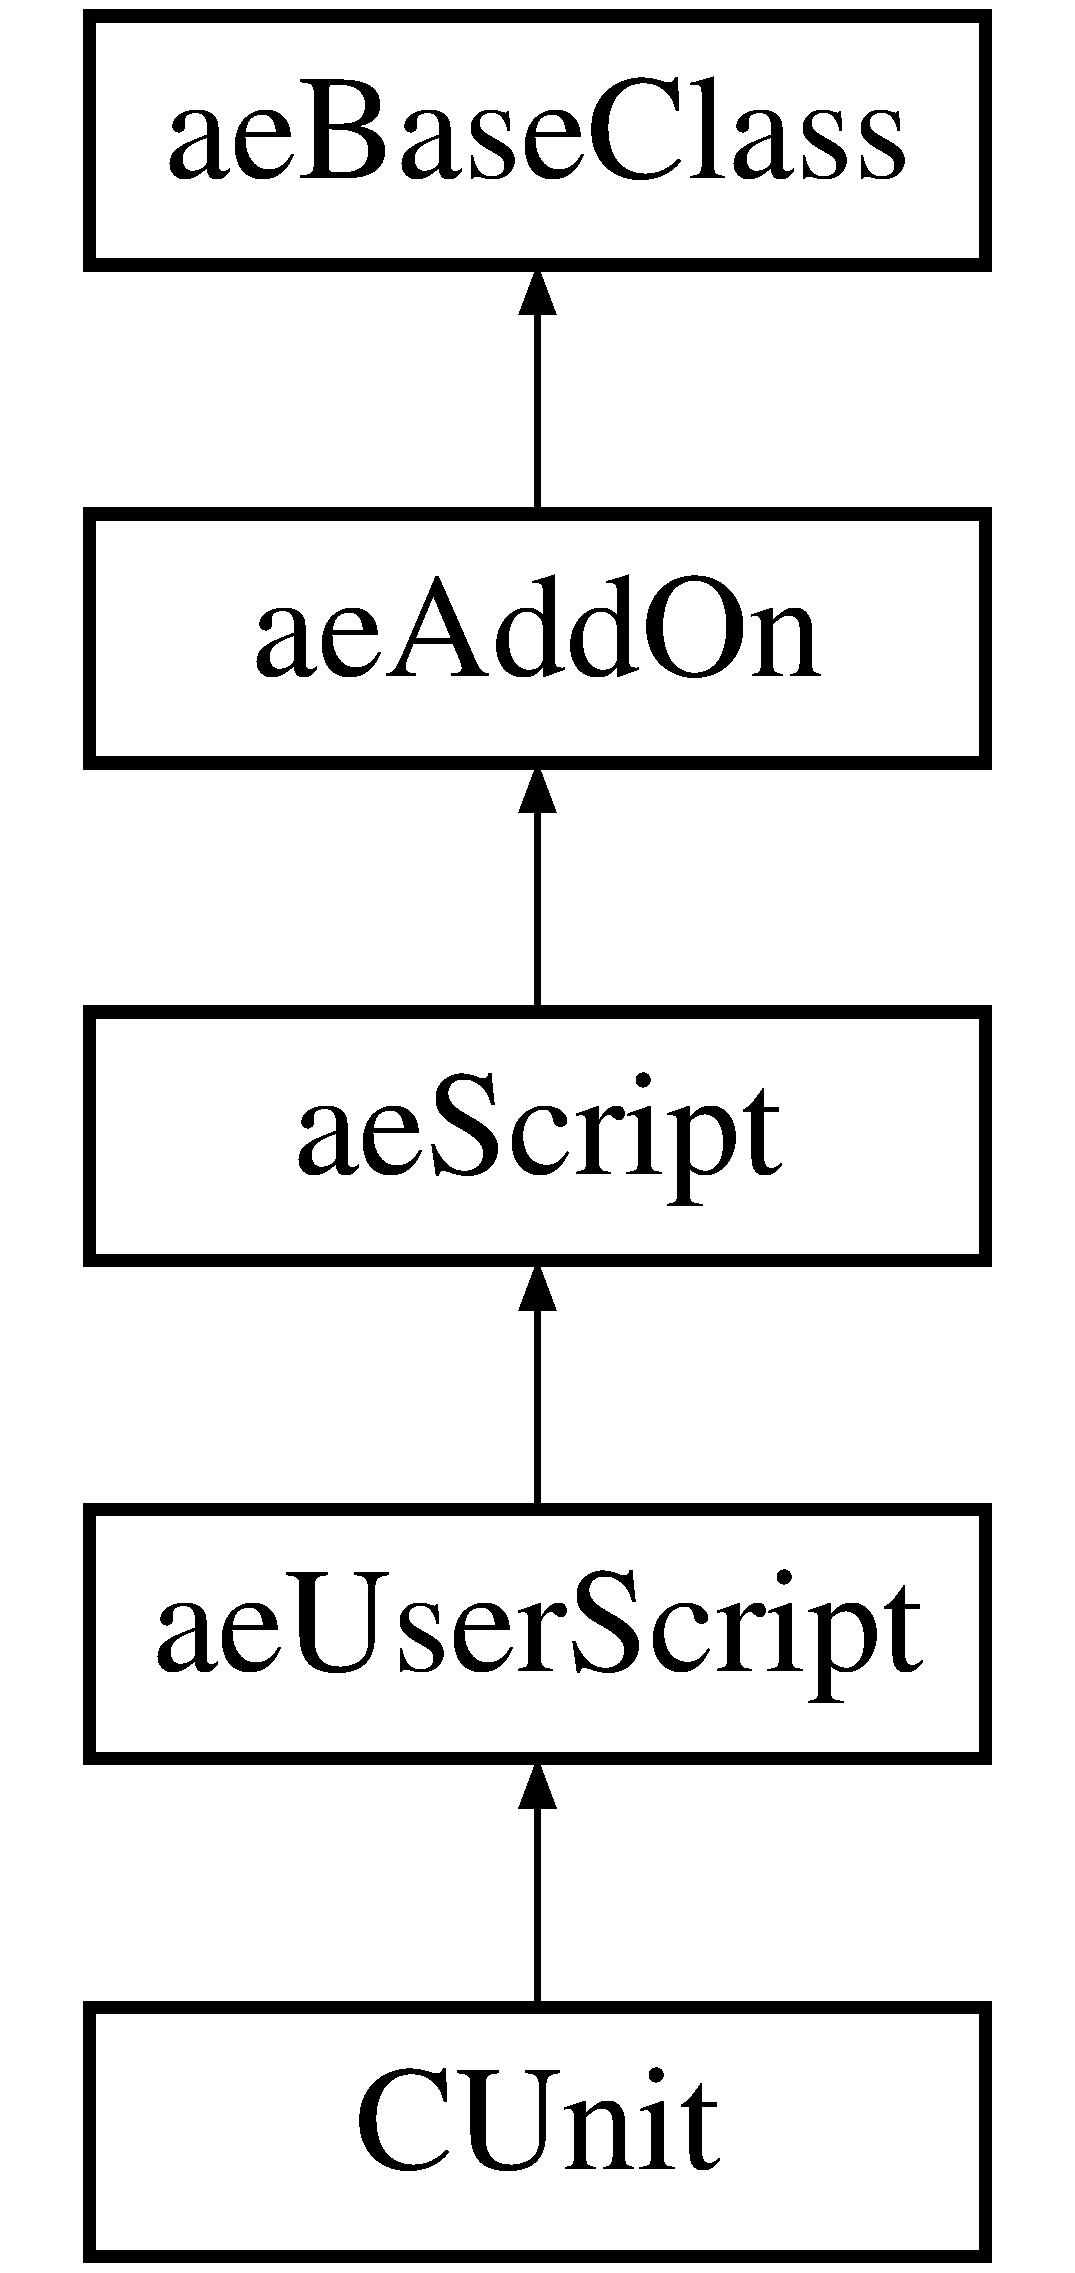
\includegraphics[height=5.000000cm]{classae_user_script}
\end{center}
\end{figure}
\subsection*{Public Member Functions}
\begin{DoxyCompactItemize}
\item 
int \hyperlink{classae_user_script_a53400e3f0443470e8570ec3218c9a051}{Get\+User\+Script\+Id} ()
\begin{DoxyCompactList}\small\item\em Gets user script identifier. \end{DoxyCompactList}\end{DoxyCompactItemize}
\subsection*{Protected Attributes}
\begin{DoxyCompactItemize}
\item 
int {\bfseries m\+\_\+n\+User\+Script\+ID}\hypertarget{classae_user_script_a3b7e57c1b556b768efcaa2fa494bd764}{}\label{classae_user_script_a3b7e57c1b556b768efcaa2fa494bd764}

\end{DoxyCompactItemize}


\subsection{Detailed Description}
An user script. 

\subsection{Member Function Documentation}
\index{ae\+User\+Script@{ae\+User\+Script}!Get\+User\+Script\+Id@{Get\+User\+Script\+Id}}
\index{Get\+User\+Script\+Id@{Get\+User\+Script\+Id}!ae\+User\+Script@{ae\+User\+Script}}
\subsubsection[{\texorpdfstring{Get\+User\+Script\+Id()}{GetUserScriptId()}}]{\setlength{\rightskip}{0pt plus 5cm}int ae\+User\+Script\+::\+Get\+User\+Script\+Id (
\begin{DoxyParamCaption}
{}
\end{DoxyParamCaption}
)\hspace{0.3cm}{\ttfamily [inline]}}\hypertarget{classae_user_script_a53400e3f0443470e8570ec3218c9a051}{}\label{classae_user_script_a53400e3f0443470e8570ec3218c9a051}


Gets user script identifier. 

\begin{DoxyReturn}{Returns}
The user script identifier. 
\end{DoxyReturn}


The documentation for this class was generated from the following files\+:\begin{DoxyCompactItemize}
\item 
C\+:/\+Users/\+Alvaro Estrada/\+Documents/\+Visual Studio 2015/\+Projects/\+R\+T\+S\+\_\+\+A\+E/\+R\+T\+S\+\_\+\+A\+E/\+Game/\hyperlink{_user_script_8h}{User\+Script.\+h}\item 
C\+:/\+Users/\+Alvaro Estrada/\+Documents/\+Visual Studio 2015/\+Projects/\+R\+T\+S\+\_\+\+A\+E/\+R\+T\+S\+\_\+\+A\+E/\+Game/User\+Script.\+cpp\end{DoxyCompactItemize}

\hypertarget{structae_core_1_1ae_vector2}{}\section{ae\+Core\+:\+:ae\+Vector2 Struct Reference}
\label{structae_core_1_1ae_vector2}\index{ae\+Core\+::ae\+Vector2@{ae\+Core\+::ae\+Vector2}}


This structure purpose is to make mathematical operations in a 2 dimensional space.  




{\ttfamily \#include $<$Vector2.\+h$>$}

\subsection*{Public Member Functions}
\begin{DoxyCompactItemize}
\item 
\hyperlink{structae_core_1_1ae_vector2_ac5c856b5234ac30db8ec5b2e16fcc917}{ae\+Vector2} (const \hyperlink{structae_core_1_1ae_vector2}{ae\+Vector2} \&V)\hypertarget{structae_core_1_1ae_vector2_ac5c856b5234ac30db8ec5b2e16fcc917}{}\label{structae_core_1_1ae_vector2_ac5c856b5234ac30db8ec5b2e16fcc917}

\begin{DoxyCompactList}\small\item\em Receives another vector and copies its values. \end{DoxyCompactList}\item 
\hyperlink{structae_core_1_1ae_vector2_aefdaa829e69d7ee0b409c6eae7c00988}{ae\+Vector2} (float X, float Y)\hypertarget{structae_core_1_1ae_vector2_aefdaa829e69d7ee0b409c6eae7c00988}{}\label{structae_core_1_1ae_vector2_aefdaa829e69d7ee0b409c6eae7c00988}

\begin{DoxyCompactList}\small\item\em Receives the X and Y values. \end{DoxyCompactList}\item 
\hyperlink{structae_core_1_1ae_vector2}{ae\+Vector2} {\bfseries operator$\ast$} (\hyperlink{structae_core_1_1ae_vector2}{ae\+Vector2} \&V)\hypertarget{structae_core_1_1ae_vector2_a35dee1169b3fcb4d18a6e964f974fdfa}{}\label{structae_core_1_1ae_vector2_a35dee1169b3fcb4d18a6e964f974fdfa}

\item 
\hyperlink{structae_core_1_1ae_vector2}{ae\+Vector2} {\bfseries operator+} (\hyperlink{structae_core_1_1ae_vector2}{ae\+Vector2} \&V)\hypertarget{structae_core_1_1ae_vector2_a1f05fc5f463024521ae0e4567450f323}{}\label{structae_core_1_1ae_vector2_a1f05fc5f463024521ae0e4567450f323}

\item 
\hyperlink{structae_core_1_1ae_vector2}{ae\+Vector2} {\bfseries operator-\/} (\hyperlink{structae_core_1_1ae_vector2}{ae\+Vector2} \&V)\hypertarget{structae_core_1_1ae_vector2_a64c45c3dbbcb94a651dc7bf25c57b35e}{}\label{structae_core_1_1ae_vector2_a64c45c3dbbcb94a651dc7bf25c57b35e}

\item 
\hyperlink{structae_core_1_1ae_vector2}{ae\+Vector2} {\bfseries operator/} (\hyperlink{structae_core_1_1ae_vector2}{ae\+Vector2} \&V)\hypertarget{structae_core_1_1ae_vector2_aa10a1c43af83b5afb0f602d0c33bd020}{}\label{structae_core_1_1ae_vector2_aa10a1c43af83b5afb0f602d0c33bd020}

\item 
\hyperlink{structae_core_1_1ae_vector2}{ae\+Vector2} {\bfseries operator$\ast$} (float S)\hypertarget{structae_core_1_1ae_vector2_a0222825ed9080e04c30f16ba5b3c8718}{}\label{structae_core_1_1ae_vector2_a0222825ed9080e04c30f16ba5b3c8718}

\item 
\hyperlink{structae_core_1_1ae_vector2}{ae\+Vector2} {\bfseries operator/} (float S)\hypertarget{structae_core_1_1ae_vector2_a1ddda84865144e75290a893d26a29c94}{}\label{structae_core_1_1ae_vector2_a1ddda84865144e75290a893d26a29c94}

\item 
float \hyperlink{structae_core_1_1ae_vector2_a83ab1efd48119f2296300afea3205175}{operator$\vert$} (\hyperlink{structae_core_1_1ae_vector2}{ae\+Vector2} \&V)\hypertarget{structae_core_1_1ae_vector2_a83ab1efd48119f2296300afea3205175}{}\label{structae_core_1_1ae_vector2_a83ab1efd48119f2296300afea3205175}

\begin{DoxyCompactList}\small\item\em Is the same as using the dot product function. \end{DoxyCompactList}\item 
float \hyperlink{structae_core_1_1ae_vector2_a710a67ece33589ed785d2b5cdcb14e7b}{operator$^\wedge$} (\hyperlink{structae_core_1_1ae_vector2}{ae\+Vector2} \&V)\hypertarget{structae_core_1_1ae_vector2_a710a67ece33589ed785d2b5cdcb14e7b}{}\label{structae_core_1_1ae_vector2_a710a67ece33589ed785d2b5cdcb14e7b}

\begin{DoxyCompactList}\small\item\em Is the same as using the cross product function. \end{DoxyCompactList}\item 
\hyperlink{structae_core_1_1ae_vector2}{ae\+Vector2} \& {\bfseries operator+=} (\hyperlink{structae_core_1_1ae_vector2}{ae\+Vector2} \&V)\hypertarget{structae_core_1_1ae_vector2_a8c14d01447decc372de45d1b78ccf02a}{}\label{structae_core_1_1ae_vector2_a8c14d01447decc372de45d1b78ccf02a}

\item 
\hyperlink{structae_core_1_1ae_vector2}{ae\+Vector2} \& {\bfseries operator-\/=} (\hyperlink{structae_core_1_1ae_vector2}{ae\+Vector2} \&V)\hypertarget{structae_core_1_1ae_vector2_ac2a6f632bee4dc7ed37e74da97ae567e}{}\label{structae_core_1_1ae_vector2_ac2a6f632bee4dc7ed37e74da97ae567e}

\item 
\hyperlink{structae_core_1_1ae_vector2}{ae\+Vector2} \& {\bfseries operator$\ast$=} (\hyperlink{structae_core_1_1ae_vector2}{ae\+Vector2} \&V)\hypertarget{structae_core_1_1ae_vector2_ad4d7c5d19803973528c3902aae9d4051}{}\label{structae_core_1_1ae_vector2_ad4d7c5d19803973528c3902aae9d4051}

\item 
\hyperlink{structae_core_1_1ae_vector2}{ae\+Vector2} \& {\bfseries operator/=} (\hyperlink{structae_core_1_1ae_vector2}{ae\+Vector2} \&V)\hypertarget{structae_core_1_1ae_vector2_a82f4a55bc9e25813a2acd55d68257ef6}{}\label{structae_core_1_1ae_vector2_a82f4a55bc9e25813a2acd55d68257ef6}

\item 
\hyperlink{structae_core_1_1ae_vector2}{ae\+Vector2} \& {\bfseries operator$\ast$=} (float S)\hypertarget{structae_core_1_1ae_vector2_ac53710e51b3adcd4f755d575cdaea65a}{}\label{structae_core_1_1ae_vector2_ac53710e51b3adcd4f755d575cdaea65a}

\item 
\hyperlink{structae_core_1_1ae_vector2}{ae\+Vector2} \& {\bfseries operator/=} (float S)\hypertarget{structae_core_1_1ae_vector2_a9d0bea3d44ca4eb76faa59d0e95855b5}{}\label{structae_core_1_1ae_vector2_a9d0bea3d44ca4eb76faa59d0e95855b5}

\item 
bool {\bfseries operator==} (\hyperlink{structae_core_1_1ae_vector2}{ae\+Vector2} \&V)\hypertarget{structae_core_1_1ae_vector2_a3e369a57571f837fd0455bdef342e434}{}\label{structae_core_1_1ae_vector2_a3e369a57571f837fd0455bdef342e434}

\item 
bool {\bfseries operator!=} (\hyperlink{structae_core_1_1ae_vector2}{ae\+Vector2} \&V)\hypertarget{structae_core_1_1ae_vector2_ab800f8ac2b541c2e030da652c656ecdd}{}\label{structae_core_1_1ae_vector2_ab800f8ac2b541c2e030da652c656ecdd}

\item 
bool \hyperlink{structae_core_1_1ae_vector2_a0439b7ae75d42d3cc97b8b6ab75d2f4e}{Close\+Enough} (\hyperlink{structae_core_1_1ae_vector2}{ae\+Vector2} \&V, float Range)
\begin{DoxyCompactList}\small\item\em It says if a point is close enough of another point. \end{DoxyCompactList}\item 
float \hyperlink{structae_core_1_1ae_vector2_a8f0a5de82a0f29a407acb9c2ed235e44}{Magnitude} ()
\begin{DoxyCompactList}\small\item\em Returns the scalar value of the vector in form of a floating number. \end{DoxyCompactList}\item 
float \hyperlink{structae_core_1_1ae_vector2_a76c28b0e51ec3b5465d9906f816480ad}{Dot\+Product} (\hyperlink{structae_core_1_1ae_vector2}{ae\+Vector2} \&V)
\begin{DoxyCompactList}\small\item\em Returns the sum of the products of the corresponding entries. \end{DoxyCompactList}\item 
float \hyperlink{structae_core_1_1ae_vector2_a64aa61dda394f53cc1c431af1f97cca7}{Angle\+Between\+Vectors} (\hyperlink{structae_core_1_1ae_vector2}{ae\+Vector2} \&V)
\begin{DoxyCompactList}\small\item\em Returns the angle between vectors in rads. \end{DoxyCompactList}\item 
float \hyperlink{structae_core_1_1ae_vector2_a3568b61e4b6c113f2343e0050ea0fe9c}{Cross\+Product} (\hyperlink{structae_core_1_1ae_vector2}{ae\+Vector2} \&V)
\begin{DoxyCompactList}\small\item\em Returns the value of the resulting vector that is perpendicular to both entries, with a direction given by the right -\/ hand rule and a magnitude equal to the area of the parallelogram that the vectors span. \end{DoxyCompactList}\item 
float \hyperlink{structae_core_1_1ae_vector2_ab69650579a4fcdf0259eac57372923d5}{Scalar\+Projection} (\hyperlink{structae_core_1_1ae_vector2}{ae\+Vector2} \&V)
\begin{DoxyCompactList}\small\item\em Returns the magnitude of the shadow left by another vector on top of this vector. \end{DoxyCompactList}\item 
\hyperlink{structae_core_1_1ae_vector2}{ae\+Vector2} \hyperlink{structae_core_1_1ae_vector2_a1e35d976770bb33f7c71610d60f39b57}{Normalize} ()
\begin{DoxyCompactList}\small\item\em Returns the direction of this vector. \end{DoxyCompactList}\item 
\hyperlink{structae_core_1_1ae_vector2}{ae\+Vector2} \hyperlink{structae_core_1_1ae_vector2_ae625d90bf8198595928663434dd24a87}{Vector\+Projection} (\hyperlink{structae_core_1_1ae_vector2}{ae\+Vector2} \&V)
\begin{DoxyCompactList}\small\item\em Returns the shadow left by another vector on top of this vector. \end{DoxyCompactList}\end{DoxyCompactItemize}
\subsection*{Public Attributes}
\begin{DoxyCompactItemize}
\item 
float {\bfseries x}\hypertarget{structae_core_1_1ae_vector2_a0e26a2527248bad24e9e2fcb451c381e}{}\label{structae_core_1_1ae_vector2_a0e26a2527248bad24e9e2fcb451c381e}

\item 
float {\bfseries y}\hypertarget{structae_core_1_1ae_vector2_acdd8de4847b1b8f2ff340bc00a646a62}{}\label{structae_core_1_1ae_vector2_acdd8de4847b1b8f2ff340bc00a646a62}

\end{DoxyCompactItemize}


\subsection{Detailed Description}
This structure purpose is to make mathematical operations in a 2 dimensional space. 

\begin{DoxyAuthor}{Author}
Alvaro Estrada 
\end{DoxyAuthor}
\begin{DoxyDate}{Date}
14/05/2016 
\end{DoxyDate}


\subsection{Member Function Documentation}
\index{ae\+Core\+::ae\+Vector2@{ae\+Core\+::ae\+Vector2}!Angle\+Between\+Vectors@{Angle\+Between\+Vectors}}
\index{Angle\+Between\+Vectors@{Angle\+Between\+Vectors}!ae\+Core\+::ae\+Vector2@{ae\+Core\+::ae\+Vector2}}
\subsubsection[{\texorpdfstring{Angle\+Between\+Vectors(ae\+Vector2 \&\+V)}{AngleBetweenVectors(aeVector2 &V)}}]{\setlength{\rightskip}{0pt plus 5cm}float ae\+Core\+::ae\+Vector2\+::\+Angle\+Between\+Vectors (
\begin{DoxyParamCaption}
\item[{{\bf ae\+Vector2} \&}]{V}
\end{DoxyParamCaption}
)}\hypertarget{structae_core_1_1ae_vector2_a64aa61dda394f53cc1c431af1f97cca7}{}\label{structae_core_1_1ae_vector2_a64aa61dda394f53cc1c431af1f97cca7}


Returns the angle between vectors in rads. 


\begin{DoxyParams}[1]{Parameters}
\mbox{\tt in,out}  & {\em V} & The \hyperlink{structae_core_1_1ae_vector2}{ae\+Vector2} to process.\\
\hline
\end{DoxyParams}
\begin{DoxyReturn}{Returns}
A float. 
\end{DoxyReturn}
It gets the angle by using the definition of the dot product, and gives it direction getting the orientation given by the sign of the cross product. \index{ae\+Core\+::ae\+Vector2@{ae\+Core\+::ae\+Vector2}!Close\+Enough@{Close\+Enough}}
\index{Close\+Enough@{Close\+Enough}!ae\+Core\+::ae\+Vector2@{ae\+Core\+::ae\+Vector2}}
\subsubsection[{\texorpdfstring{Close\+Enough(ae\+Vector2 \&\+V, float Range)}{CloseEnough(aeVector2 &V, float Range)}}]{\setlength{\rightskip}{0pt plus 5cm}bool ae\+Core\+::ae\+Vector2\+::\+Close\+Enough (
\begin{DoxyParamCaption}
\item[{{\bf ae\+Vector2} \&}]{V, }
\item[{float}]{Range}
\end{DoxyParamCaption}
)}\hypertarget{structae_core_1_1ae_vector2_a0439b7ae75d42d3cc97b8b6ab75d2f4e}{}\label{structae_core_1_1ae_vector2_a0439b7ae75d42d3cc97b8b6ab75d2f4e}


It says if a point is close enough of another point. 


\begin{DoxyParams}[1]{Parameters}
\mbox{\tt in,out}  & {\em V} & The \hyperlink{structae_core_1_1ae_vector2}{ae\+Vector2} to process. \\
\hline
 & {\em Range} & The range.\\
\hline
\end{DoxyParams}
\begin{DoxyReturn}{Returns}
true if it\textquotesingle{}s close enough, false if it\textquotesingle{}s too far
\end{DoxyReturn}
Returns true if the magnitude between vectors is lower than the asked range. \index{ae\+Core\+::ae\+Vector2@{ae\+Core\+::ae\+Vector2}!Cross\+Product@{Cross\+Product}}
\index{Cross\+Product@{Cross\+Product}!ae\+Core\+::ae\+Vector2@{ae\+Core\+::ae\+Vector2}}
\subsubsection[{\texorpdfstring{Cross\+Product(ae\+Vector2 \&\+V)}{CrossProduct(aeVector2 &V)}}]{\setlength{\rightskip}{0pt plus 5cm}float ae\+Core\+::ae\+Vector2\+::\+Cross\+Product (
\begin{DoxyParamCaption}
\item[{{\bf ae\+Vector2} \&}]{V}
\end{DoxyParamCaption}
)}\hypertarget{structae_core_1_1ae_vector2_a3568b61e4b6c113f2343e0050ea0fe9c}{}\label{structae_core_1_1ae_vector2_a3568b61e4b6c113f2343e0050ea0fe9c}


Returns the value of the resulting vector that is perpendicular to both entries, with a direction given by the right -\/ hand rule and a magnitude equal to the area of the parallelogram that the vectors span. 


\begin{DoxyParams}[1]{Parameters}
\mbox{\tt in,out}  & {\em V} & The \hyperlink{structae_core_1_1ae_vector2}{ae\+Vector2} to process.\\
\hline
\end{DoxyParams}
\begin{DoxyReturn}{Returns}
A float. 
\end{DoxyReturn}
The cross product is the value of the resulting vector that is perpendicular to both entries, with a direction given by the right -\/ hand rule and a magnitude equal to the area of the parallelogram that the vectors span. \index{ae\+Core\+::ae\+Vector2@{ae\+Core\+::ae\+Vector2}!Dot\+Product@{Dot\+Product}}
\index{Dot\+Product@{Dot\+Product}!ae\+Core\+::ae\+Vector2@{ae\+Core\+::ae\+Vector2}}
\subsubsection[{\texorpdfstring{Dot\+Product(ae\+Vector2 \&\+V)}{DotProduct(aeVector2 &V)}}]{\setlength{\rightskip}{0pt plus 5cm}float ae\+Core\+::ae\+Vector2\+::\+Dot\+Product (
\begin{DoxyParamCaption}
\item[{{\bf ae\+Vector2} \&}]{V}
\end{DoxyParamCaption}
)}\hypertarget{structae_core_1_1ae_vector2_a76c28b0e51ec3b5465d9906f816480ad}{}\label{structae_core_1_1ae_vector2_a76c28b0e51ec3b5465d9906f816480ad}


Returns the sum of the products of the corresponding entries. 


\begin{DoxyParams}[1]{Parameters}
\mbox{\tt in,out}  & {\em V} & The \hyperlink{structae_core_1_1ae_vector2}{ae\+Vector2} to process.\\
\hline
\end{DoxyParams}
\begin{DoxyReturn}{Returns}
A float. 
\end{DoxyReturn}
The dot product is the result of the sum of the products of the corresponding entries of the two sequences of numbers. \index{ae\+Core\+::ae\+Vector2@{ae\+Core\+::ae\+Vector2}!Magnitude@{Magnitude}}
\index{Magnitude@{Magnitude}!ae\+Core\+::ae\+Vector2@{ae\+Core\+::ae\+Vector2}}
\subsubsection[{\texorpdfstring{Magnitude()}{Magnitude()}}]{\setlength{\rightskip}{0pt plus 5cm}float ae\+Core\+::ae\+Vector2\+::\+Magnitude (
\begin{DoxyParamCaption}
{}
\end{DoxyParamCaption}
)}\hypertarget{structae_core_1_1ae_vector2_a8f0a5de82a0f29a407acb9c2ed235e44}{}\label{structae_core_1_1ae_vector2_a8f0a5de82a0f29a407acb9c2ed235e44}


Returns the scalar value of the vector in form of a floating number. 

\begin{DoxyReturn}{Returns}
A float. 
\end{DoxyReturn}
The magnitude of the vector is the length of the vector, it is obtained by the square root of the addition of the squared values of x and y. \index{ae\+Core\+::ae\+Vector2@{ae\+Core\+::ae\+Vector2}!Normalize@{Normalize}}
\index{Normalize@{Normalize}!ae\+Core\+::ae\+Vector2@{ae\+Core\+::ae\+Vector2}}
\subsubsection[{\texorpdfstring{Normalize()}{Normalize()}}]{\setlength{\rightskip}{0pt plus 5cm}{\bf ae\+Vector2} ae\+Core\+::ae\+Vector2\+::\+Normalize (
\begin{DoxyParamCaption}
{}
\end{DoxyParamCaption}
)}\hypertarget{structae_core_1_1ae_vector2_a1e35d976770bb33f7c71610d60f39b57}{}\label{structae_core_1_1ae_vector2_a1e35d976770bb33f7c71610d60f39b57}


Returns the direction of this vector. 

\begin{DoxyReturn}{Returns}
A \hyperlink{structae_core_1_1ae_vector2}{ae\+Vector2}. 
\end{DoxyReturn}
The normalized vector is a vector in the same direction but with a magnitude equals to one \index{ae\+Core\+::ae\+Vector2@{ae\+Core\+::ae\+Vector2}!Scalar\+Projection@{Scalar\+Projection}}
\index{Scalar\+Projection@{Scalar\+Projection}!ae\+Core\+::ae\+Vector2@{ae\+Core\+::ae\+Vector2}}
\subsubsection[{\texorpdfstring{Scalar\+Projection(ae\+Vector2 \&\+V)}{ScalarProjection(aeVector2 &V)}}]{\setlength{\rightskip}{0pt plus 5cm}float ae\+Core\+::ae\+Vector2\+::\+Scalar\+Projection (
\begin{DoxyParamCaption}
\item[{{\bf ae\+Vector2} \&}]{V}
\end{DoxyParamCaption}
)}\hypertarget{structae_core_1_1ae_vector2_ab69650579a4fcdf0259eac57372923d5}{}\label{structae_core_1_1ae_vector2_ab69650579a4fcdf0259eac57372923d5}


Returns the magnitude of the shadow left by another vector on top of this vector. 


\begin{DoxyParams}[1]{Parameters}
\mbox{\tt in,out}  & {\em V} & The \hyperlink{structae_core_1_1ae_vector2}{ae\+Vector2} to process.\\
\hline
\end{DoxyParams}
\begin{DoxyReturn}{Returns}
A float. 
\end{DoxyReturn}
The scalar projection is a scalar, equal to the length of the orthogonal projection of A on B, with a negative sign if the projection has an opposite direction with respect to B. \index{ae\+Core\+::ae\+Vector2@{ae\+Core\+::ae\+Vector2}!Vector\+Projection@{Vector\+Projection}}
\index{Vector\+Projection@{Vector\+Projection}!ae\+Core\+::ae\+Vector2@{ae\+Core\+::ae\+Vector2}}
\subsubsection[{\texorpdfstring{Vector\+Projection(ae\+Vector2 \&\+V)}{VectorProjection(aeVector2 &V)}}]{\setlength{\rightskip}{0pt plus 5cm}{\bf ae\+Vector2} ae\+Core\+::ae\+Vector2\+::\+Vector\+Projection (
\begin{DoxyParamCaption}
\item[{{\bf ae\+Vector2} \&}]{V}
\end{DoxyParamCaption}
)}\hypertarget{structae_core_1_1ae_vector2_ae625d90bf8198595928663434dd24a87}{}\label{structae_core_1_1ae_vector2_ae625d90bf8198595928663434dd24a87}


Returns the shadow left by another vector on top of this vector. 


\begin{DoxyParams}[1]{Parameters}
\mbox{\tt in,out}  & {\em V} & The \hyperlink{structae_core_1_1ae_vector2}{ae\+Vector2} to process.\\
\hline
\end{DoxyParams}
\begin{DoxyReturn}{Returns}
A \hyperlink{structae_core_1_1ae_vector2}{ae\+Vector2}. 
\end{DoxyReturn}
The vector projection of A on B is a vector whose magnitude is the scalar projection of A on B and whose angle against B. 

The documentation for this struct was generated from the following files\+:\begin{DoxyCompactItemize}
\item 
C\+:/\+Users/\+Alvaro Estrada/\+Documents/\+Visual Studio 2015/\+Projects/\+R\+T\+S\+\_\+\+A\+E/ae\+Core/\+Math/Vector2.\+h\item 
C\+:/\+Users/\+Alvaro Estrada/\+Documents/\+Visual Studio 2015/\+Projects/\+R\+T\+S\+\_\+\+A\+E/ae\+Core/\+Math/Vector2.\+cpp\end{DoxyCompactItemize}

\hypertarget{structae_core_1_1ae_vector3}{}\section{ae\+Core\+:\+:ae\+Vector3 Struct Reference}
\label{structae_core_1_1ae_vector3}\index{ae\+Core\+::ae\+Vector3@{ae\+Core\+::ae\+Vector3}}


This structure purpose is to make mathematical operations in a 3 dimensional space.  




{\ttfamily \#include $<$Vector3.\+h$>$}

\subsection*{Public Member Functions}
\begin{DoxyCompactItemize}
\item 
\hyperlink{structae_core_1_1ae_vector3_a1bffd7fb87e70d793f579c7d29fd965f}{ae\+Vector3} (const \hyperlink{structae_core_1_1ae_vector3}{ae\+Vector3} \&V)\hypertarget{structae_core_1_1ae_vector3_a1bffd7fb87e70d793f579c7d29fd965f}{}\label{structae_core_1_1ae_vector3_a1bffd7fb87e70d793f579c7d29fd965f}

\begin{DoxyCompactList}\small\item\em Receives another vector and copies its values. \end{DoxyCompactList}\item 
\hyperlink{structae_core_1_1ae_vector3_a2ad1a3d5e07aef4887e48eced217d3b0}{ae\+Vector3} (float X, float Y=0, float Z=0)\hypertarget{structae_core_1_1ae_vector3_a2ad1a3d5e07aef4887e48eced217d3b0}{}\label{structae_core_1_1ae_vector3_a2ad1a3d5e07aef4887e48eced217d3b0}

\begin{DoxyCompactList}\small\item\em Receives the X, Y and Z values. \end{DoxyCompactList}\item 
\hyperlink{structae_core_1_1ae_vector3}{ae\+Vector3} {\bfseries operator$\ast$} (\hyperlink{structae_core_1_1ae_vector3}{ae\+Vector3} \&V)\hypertarget{structae_core_1_1ae_vector3_ad0e245d1fdbb5b3187dcb30353cc2e35}{}\label{structae_core_1_1ae_vector3_ad0e245d1fdbb5b3187dcb30353cc2e35}

\item 
\hyperlink{structae_core_1_1ae_vector3}{ae\+Vector3} {\bfseries operator+} (\hyperlink{structae_core_1_1ae_vector3}{ae\+Vector3} \&V)\hypertarget{structae_core_1_1ae_vector3_a3a61eeb0433d2780778c111e3e374f54}{}\label{structae_core_1_1ae_vector3_a3a61eeb0433d2780778c111e3e374f54}

\item 
\hyperlink{structae_core_1_1ae_vector3}{ae\+Vector3} {\bfseries operator-\/} (\hyperlink{structae_core_1_1ae_vector3}{ae\+Vector3} \&V)\hypertarget{structae_core_1_1ae_vector3_a046428bb551a023ed5d332dd8c947beb}{}\label{structae_core_1_1ae_vector3_a046428bb551a023ed5d332dd8c947beb}

\item 
\hyperlink{structae_core_1_1ae_vector3}{ae\+Vector3} {\bfseries operator/} (\hyperlink{structae_core_1_1ae_vector3}{ae\+Vector3} \&V)\hypertarget{structae_core_1_1ae_vector3_ad98c6598070d46eb8e6d1611ac6809d2}{}\label{structae_core_1_1ae_vector3_ad98c6598070d46eb8e6d1611ac6809d2}

\item 
\hyperlink{structae_core_1_1ae_vector3}{ae\+Vector3} {\bfseries operator$\ast$} (float S)\hypertarget{structae_core_1_1ae_vector3_a823b323533ad9b66ff4033e847ce896b}{}\label{structae_core_1_1ae_vector3_a823b323533ad9b66ff4033e847ce896b}

\item 
\hyperlink{structae_core_1_1ae_vector3}{ae\+Vector3} {\bfseries operator/} (float S)\hypertarget{structae_core_1_1ae_vector3_a583a2a73944a2886d58681a681c55128}{}\label{structae_core_1_1ae_vector3_a583a2a73944a2886d58681a681c55128}

\item 
bool {\bfseries operator==} (\hyperlink{structae_core_1_1ae_vector3}{ae\+Vector3} \&V)\hypertarget{structae_core_1_1ae_vector3_afe97eb2655083afd9de9ca55ada5a0a5}{}\label{structae_core_1_1ae_vector3_afe97eb2655083afd9de9ca55ada5a0a5}

\item 
bool {\bfseries operator!=} (\hyperlink{structae_core_1_1ae_vector3}{ae\+Vector3} \&V)\hypertarget{structae_core_1_1ae_vector3_a83af9d9eac68fd3cc21b85a53d7a57e2}{}\label{structae_core_1_1ae_vector3_a83af9d9eac68fd3cc21b85a53d7a57e2}

\item 
\hyperlink{structae_core_1_1ae_vector3}{ae\+Vector3} \& {\bfseries operator+=} (\hyperlink{structae_core_1_1ae_vector3}{ae\+Vector3} \&V)\hypertarget{structae_core_1_1ae_vector3_a4145cb486fe6fa5286510fddcd85711c}{}\label{structae_core_1_1ae_vector3_a4145cb486fe6fa5286510fddcd85711c}

\item 
\hyperlink{structae_core_1_1ae_vector3}{ae\+Vector3} \& {\bfseries operator-\/=} (\hyperlink{structae_core_1_1ae_vector3}{ae\+Vector3} \&V)\hypertarget{structae_core_1_1ae_vector3_ac3dc6b3ba47d822b01088f31076589db}{}\label{structae_core_1_1ae_vector3_ac3dc6b3ba47d822b01088f31076589db}

\item 
\hyperlink{structae_core_1_1ae_vector3}{ae\+Vector3} \& {\bfseries operator$\ast$=} (\hyperlink{structae_core_1_1ae_vector3}{ae\+Vector3} \&V)\hypertarget{structae_core_1_1ae_vector3_a8a04815bab18f2a64398dc1e691976c9}{}\label{structae_core_1_1ae_vector3_a8a04815bab18f2a64398dc1e691976c9}

\item 
\hyperlink{structae_core_1_1ae_vector3}{ae\+Vector3} \& {\bfseries operator/=} (\hyperlink{structae_core_1_1ae_vector3}{ae\+Vector3} \&V)\hypertarget{structae_core_1_1ae_vector3_a3fb20008b3f9c28ca4cb8863dccb1759}{}\label{structae_core_1_1ae_vector3_a3fb20008b3f9c28ca4cb8863dccb1759}

\item 
\hyperlink{structae_core_1_1ae_vector3}{ae\+Vector3} \& {\bfseries operator$\ast$=} (float S)\hypertarget{structae_core_1_1ae_vector3_aedba8c35c5bdb6b1045b8042d09640ad}{}\label{structae_core_1_1ae_vector3_aedba8c35c5bdb6b1045b8042d09640ad}

\item 
\hyperlink{structae_core_1_1ae_vector3}{ae\+Vector3} \& {\bfseries operator/=} (float S)\hypertarget{structae_core_1_1ae_vector3_ae6c0bdb11ad31d512256ae07e1bd99c8}{}\label{structae_core_1_1ae_vector3_ae6c0bdb11ad31d512256ae07e1bd99c8}

\item 
bool \hyperlink{structae_core_1_1ae_vector3_a5a196d2e3ece1eb67de18e0dd8fbe0f0}{Close\+Enough} (\hyperlink{structae_core_1_1ae_vector3}{ae\+Vector3} \&V, float Range)
\begin{DoxyCompactList}\small\item\em It says if a point is close enough of another point. \end{DoxyCompactList}\item 
float \hyperlink{structae_core_1_1ae_vector3_add758370b650c955432048f711e3e4b2}{Magnitude} ()
\begin{DoxyCompactList}\small\item\em Return the scalar value of the vector in form of a floating number. \end{DoxyCompactList}\item 
float \hyperlink{structae_core_1_1ae_vector3_a181070166a463a9622a562341f62bdb2}{Dot\+Product} (\hyperlink{structae_core_1_1ae_vector3}{ae\+Vector3} \&V)
\begin{DoxyCompactList}\small\item\em Returns the dot product between this vector and the input. \end{DoxyCompactList}\item 
float \hyperlink{structae_core_1_1ae_vector3_a469e4d42ba109c4f1077434a7a97792a}{Angle\+Between\+Vectors} (\hyperlink{structae_core_1_1ae_vector3}{ae\+Vector3} \&V)
\begin{DoxyCompactList}\small\item\em Returns the angle between vectors. \end{DoxyCompactList}\item 
float \hyperlink{structae_core_1_1ae_vector3_abebbe7583cf4bcf08da988f4f72e6c84}{Cross2\+Product} (\hyperlink{structae_core_1_1ae_vector3}{ae\+Vector3} \&V)
\begin{DoxyCompactList}\small\item\em Returns the cross product between vectors as they were 2D. \end{DoxyCompactList}\item 
float \hyperlink{structae_core_1_1ae_vector3_a02fe6581b4ab65efbd03cd76196bd364}{Scalar\+Projection} (\hyperlink{structae_core_1_1ae_vector3}{ae\+Vector3} \&V)
\begin{DoxyCompactList}\small\item\em Returns the magnitude of the shadow left by another vector on top of this vector. \end{DoxyCompactList}\item 
\hyperlink{structae_core_1_1ae_vector3}{ae\+Vector3} \hyperlink{structae_core_1_1ae_vector3_a814add51f20a124cf4fc68b2f8b3f390}{Cross3\+Product} (\hyperlink{structae_core_1_1ae_vector3}{ae\+Vector3} \&V)
\begin{DoxyCompactList}\small\item\em Returns the cross product between vectors. \end{DoxyCompactList}\item 
\hyperlink{structae_core_1_1ae_vector3}{ae\+Vector3} \hyperlink{structae_core_1_1ae_vector3_a667ef4dede390119508dc9419c36b9a4}{Normalize} ()
\begin{DoxyCompactList}\small\item\em Returns the direction of this vector. \end{DoxyCompactList}\item 
\hyperlink{structae_core_1_1ae_vector3}{ae\+Vector3} \hyperlink{structae_core_1_1ae_vector3_aed53d5d422de288adaf11003ddbc27fe}{Vector\+Projection} (\hyperlink{structae_core_1_1ae_vector3}{ae\+Vector3} \&V)
\begin{DoxyCompactList}\small\item\em Returns the shadow left by another vector on top of this vector. \end{DoxyCompactList}\item 
\hyperlink{structae_core_1_1ae_vector3}{ae\+Vector3} \hyperlink{structae_core_1_1ae_vector3_a5b3fa647aea5a516abe7cfea8353621f}{Angles\+Between\+Vectors} (\hyperlink{structae_core_1_1ae_vector3}{ae\+Vector3} \&V)
\begin{DoxyCompactList}\small\item\em Returns the angles between vectors as they were 2D. \end{DoxyCompactList}\end{DoxyCompactItemize}
\subsection*{Public Attributes}
\begin{DoxyCompactItemize}
\item 
\begin{tabbing}
xx\=xx\=xx\=xx\=xx\=xx\=xx\=xx\=xx\=\kill
union \{\\
\>struct \{\\
\>\>float {\bfseries x}\\
\>\>float {\bfseries y}\\
\>\>float {\bfseries z}\\
\>\} \hypertarget{unionae_core_1_1ae_vector3_1_1_0D26_a5594fa73c969c7c0dfbf56a710bf6c5b}{}\label{unionae_core_1_1ae_vector3_1_1_0D26_a5594fa73c969c7c0dfbf56a710bf6c5b}
\\
\>\>\>{\em A structure meant to save the array as individual values. }\\
\>float \hyperlink{structae_core_1_1ae_vector3_a273e068da49c1c595bbe877db36ce51c}{v} \mbox{[}3\mbox{]}\\
\>\>\>{\em A 3D float array. }\\
\}; \hypertarget{structae_core_1_1ae_vector3_a93f89b631e2f1dc82c718693d315f110}{}\label{structae_core_1_1ae_vector3_a93f89b631e2f1dc82c718693d315f110}
\\

\end{tabbing}\begin{DoxyCompactList}\small\item\em Is the union between X,Y and Z values and a 3D array. \end{DoxyCompactList}\end{DoxyCompactItemize}


\subsection{Detailed Description}
This structure purpose is to make mathematical operations in a 3 dimensional space. 

\begin{DoxyAuthor}{Author}
Alvaro Estrada 
\end{DoxyAuthor}
\begin{DoxyDate}{Date}
14/05/2016 
\end{DoxyDate}


\subsection{Member Function Documentation}
\index{ae\+Core\+::ae\+Vector3@{ae\+Core\+::ae\+Vector3}!Angle\+Between\+Vectors@{Angle\+Between\+Vectors}}
\index{Angle\+Between\+Vectors@{Angle\+Between\+Vectors}!ae\+Core\+::ae\+Vector3@{ae\+Core\+::ae\+Vector3}}
\subsubsection[{\texorpdfstring{Angle\+Between\+Vectors(ae\+Vector3 \&\+V)}{AngleBetweenVectors(aeVector3 &V)}}]{\setlength{\rightskip}{0pt plus 5cm}float ae\+Core\+::ae\+Vector3\+::\+Angle\+Between\+Vectors (
\begin{DoxyParamCaption}
\item[{{\bf ae\+Vector3} \&}]{V}
\end{DoxyParamCaption}
)}\hypertarget{structae_core_1_1ae_vector3_a469e4d42ba109c4f1077434a7a97792a}{}\label{structae_core_1_1ae_vector3_a469e4d42ba109c4f1077434a7a97792a}


Returns the angle between vectors. 


\begin{DoxyParams}[1]{Parameters}
\mbox{\tt in,out}  & {\em V} & The \hyperlink{structae_core_1_1ae_vector3}{ae\+Vector3} to process.\\
\hline
\end{DoxyParams}
\begin{DoxyReturn}{Returns}
A float. 
\end{DoxyReturn}
\index{ae\+Core\+::ae\+Vector3@{ae\+Core\+::ae\+Vector3}!Angles\+Between\+Vectors@{Angles\+Between\+Vectors}}
\index{Angles\+Between\+Vectors@{Angles\+Between\+Vectors}!ae\+Core\+::ae\+Vector3@{ae\+Core\+::ae\+Vector3}}
\subsubsection[{\texorpdfstring{Angles\+Between\+Vectors(ae\+Vector3 \&\+V)}{AnglesBetweenVectors(aeVector3 &V)}}]{\setlength{\rightskip}{0pt plus 5cm}{\bf ae\+Vector3} ae\+Core\+::ae\+Vector3\+::\+Angles\+Between\+Vectors (
\begin{DoxyParamCaption}
\item[{{\bf ae\+Vector3} \&}]{V}
\end{DoxyParamCaption}
)}\hypertarget{structae_core_1_1ae_vector3_a5b3fa647aea5a516abe7cfea8353621f}{}\label{structae_core_1_1ae_vector3_a5b3fa647aea5a516abe7cfea8353621f}


Returns the angles between vectors as they were 2D. 


\begin{DoxyParams}[1]{Parameters}
\mbox{\tt in,out}  & {\em V} & The \hyperlink{structae_core_1_1ae_vector3}{ae\+Vector3} to process.\\
\hline
\end{DoxyParams}
\begin{DoxyReturn}{Returns}
A \hyperlink{structae_core_1_1ae_vector3}{ae\+Vector3}. 
\end{DoxyReturn}
\index{ae\+Core\+::ae\+Vector3@{ae\+Core\+::ae\+Vector3}!Close\+Enough@{Close\+Enough}}
\index{Close\+Enough@{Close\+Enough}!ae\+Core\+::ae\+Vector3@{ae\+Core\+::ae\+Vector3}}
\subsubsection[{\texorpdfstring{Close\+Enough(ae\+Vector3 \&\+V, float Range)}{CloseEnough(aeVector3 &V, float Range)}}]{\setlength{\rightskip}{0pt plus 5cm}bool ae\+Core\+::ae\+Vector3\+::\+Close\+Enough (
\begin{DoxyParamCaption}
\item[{{\bf ae\+Vector3} \&}]{V, }
\item[{float}]{Range}
\end{DoxyParamCaption}
)}\hypertarget{structae_core_1_1ae_vector3_a5a196d2e3ece1eb67de18e0dd8fbe0f0}{}\label{structae_core_1_1ae_vector3_a5a196d2e3ece1eb67de18e0dd8fbe0f0}


It says if a point is close enough of another point. 


\begin{DoxyParams}[1]{Parameters}
\mbox{\tt in,out}  & {\em V} & The \hyperlink{structae_core_1_1ae_vector3}{ae\+Vector3} to process. \\
\hline
 & {\em Range} & The range.\\
\hline
\end{DoxyParams}
\begin{DoxyReturn}{Returns}
true if it\textquotesingle{}s close enough, false if it\textquotesingle{}s too far
\end{DoxyReturn}
Returns true if the magnitude between vectors is lower than the asked range. \index{ae\+Core\+::ae\+Vector3@{ae\+Core\+::ae\+Vector3}!Cross2\+Product@{Cross2\+Product}}
\index{Cross2\+Product@{Cross2\+Product}!ae\+Core\+::ae\+Vector3@{ae\+Core\+::ae\+Vector3}}
\subsubsection[{\texorpdfstring{Cross2\+Product(ae\+Vector3 \&\+V)}{Cross2Product(aeVector3 &V)}}]{\setlength{\rightskip}{0pt plus 5cm}float ae\+Core\+::ae\+Vector3\+::\+Cross2\+Product (
\begin{DoxyParamCaption}
\item[{{\bf ae\+Vector3} \&}]{V}
\end{DoxyParamCaption}
)}\hypertarget{structae_core_1_1ae_vector3_abebbe7583cf4bcf08da988f4f72e6c84}{}\label{structae_core_1_1ae_vector3_abebbe7583cf4bcf08da988f4f72e6c84}


Returns the cross product between vectors as they were 2D. 


\begin{DoxyParams}[1]{Parameters}
\mbox{\tt in,out}  & {\em V} & The \hyperlink{structae_core_1_1ae_vector3}{ae\+Vector3} to process.\\
\hline
\end{DoxyParams}
\begin{DoxyReturn}{Returns}
A float. 
\end{DoxyReturn}
\index{ae\+Core\+::ae\+Vector3@{ae\+Core\+::ae\+Vector3}!Cross3\+Product@{Cross3\+Product}}
\index{Cross3\+Product@{Cross3\+Product}!ae\+Core\+::ae\+Vector3@{ae\+Core\+::ae\+Vector3}}
\subsubsection[{\texorpdfstring{Cross3\+Product(ae\+Vector3 \&\+V)}{Cross3Product(aeVector3 &V)}}]{\setlength{\rightskip}{0pt plus 5cm}{\bf ae\+Vector3} ae\+Core\+::ae\+Vector3\+::\+Cross3\+Product (
\begin{DoxyParamCaption}
\item[{{\bf ae\+Vector3} \&}]{V}
\end{DoxyParamCaption}
)}\hypertarget{structae_core_1_1ae_vector3_a814add51f20a124cf4fc68b2f8b3f390}{}\label{structae_core_1_1ae_vector3_a814add51f20a124cf4fc68b2f8b3f390}


Returns the cross product between vectors. 


\begin{DoxyParams}[1]{Parameters}
\mbox{\tt in,out}  & {\em V} & The \hyperlink{structae_core_1_1ae_vector3}{ae\+Vector3} to process.\\
\hline
\end{DoxyParams}
\begin{DoxyReturn}{Returns}
A \hyperlink{structae_core_1_1ae_vector3}{ae\+Vector3}. 
\end{DoxyReturn}
\index{ae\+Core\+::ae\+Vector3@{ae\+Core\+::ae\+Vector3}!Dot\+Product@{Dot\+Product}}
\index{Dot\+Product@{Dot\+Product}!ae\+Core\+::ae\+Vector3@{ae\+Core\+::ae\+Vector3}}
\subsubsection[{\texorpdfstring{Dot\+Product(ae\+Vector3 \&\+V)}{DotProduct(aeVector3 &V)}}]{\setlength{\rightskip}{0pt plus 5cm}float ae\+Core\+::ae\+Vector3\+::\+Dot\+Product (
\begin{DoxyParamCaption}
\item[{{\bf ae\+Vector3} \&}]{V}
\end{DoxyParamCaption}
)}\hypertarget{structae_core_1_1ae_vector3_a181070166a463a9622a562341f62bdb2}{}\label{structae_core_1_1ae_vector3_a181070166a463a9622a562341f62bdb2}


Returns the dot product between this vector and the input. 


\begin{DoxyParams}[1]{Parameters}
\mbox{\tt in,out}  & {\em V} & The \hyperlink{structae_core_1_1ae_vector3}{ae\+Vector3} to process.\\
\hline
\end{DoxyParams}
\begin{DoxyReturn}{Returns}
A float. 
\end{DoxyReturn}
\index{ae\+Core\+::ae\+Vector3@{ae\+Core\+::ae\+Vector3}!Magnitude@{Magnitude}}
\index{Magnitude@{Magnitude}!ae\+Core\+::ae\+Vector3@{ae\+Core\+::ae\+Vector3}}
\subsubsection[{\texorpdfstring{Magnitude()}{Magnitude()}}]{\setlength{\rightskip}{0pt plus 5cm}float ae\+Core\+::ae\+Vector3\+::\+Magnitude (
\begin{DoxyParamCaption}
{}
\end{DoxyParamCaption}
)}\hypertarget{structae_core_1_1ae_vector3_add758370b650c955432048f711e3e4b2}{}\label{structae_core_1_1ae_vector3_add758370b650c955432048f711e3e4b2}


Return the scalar value of the vector in form of a floating number. 

\begin{DoxyReturn}{Returns}
A float. 
\end{DoxyReturn}
\index{ae\+Core\+::ae\+Vector3@{ae\+Core\+::ae\+Vector3}!Normalize@{Normalize}}
\index{Normalize@{Normalize}!ae\+Core\+::ae\+Vector3@{ae\+Core\+::ae\+Vector3}}
\subsubsection[{\texorpdfstring{Normalize()}{Normalize()}}]{\setlength{\rightskip}{0pt plus 5cm}{\bf ae\+Vector3} ae\+Core\+::ae\+Vector3\+::\+Normalize (
\begin{DoxyParamCaption}
{}
\end{DoxyParamCaption}
)}\hypertarget{structae_core_1_1ae_vector3_a667ef4dede390119508dc9419c36b9a4}{}\label{structae_core_1_1ae_vector3_a667ef4dede390119508dc9419c36b9a4}


Returns the direction of this vector. 

\begin{DoxyReturn}{Returns}
A \hyperlink{structae_core_1_1ae_vector3}{ae\+Vector3}. 
\end{DoxyReturn}
\index{ae\+Core\+::ae\+Vector3@{ae\+Core\+::ae\+Vector3}!Scalar\+Projection@{Scalar\+Projection}}
\index{Scalar\+Projection@{Scalar\+Projection}!ae\+Core\+::ae\+Vector3@{ae\+Core\+::ae\+Vector3}}
\subsubsection[{\texorpdfstring{Scalar\+Projection(ae\+Vector3 \&\+V)}{ScalarProjection(aeVector3 &V)}}]{\setlength{\rightskip}{0pt plus 5cm}float ae\+Core\+::ae\+Vector3\+::\+Scalar\+Projection (
\begin{DoxyParamCaption}
\item[{{\bf ae\+Vector3} \&}]{V}
\end{DoxyParamCaption}
)}\hypertarget{structae_core_1_1ae_vector3_a02fe6581b4ab65efbd03cd76196bd364}{}\label{structae_core_1_1ae_vector3_a02fe6581b4ab65efbd03cd76196bd364}


Returns the magnitude of the shadow left by another vector on top of this vector. 


\begin{DoxyParams}[1]{Parameters}
\mbox{\tt in,out}  & {\em V} & The \hyperlink{structae_core_1_1ae_vector3}{ae\+Vector3} to process.\\
\hline
\end{DoxyParams}
\begin{DoxyReturn}{Returns}
A float. 
\end{DoxyReturn}
\index{ae\+Core\+::ae\+Vector3@{ae\+Core\+::ae\+Vector3}!Vector\+Projection@{Vector\+Projection}}
\index{Vector\+Projection@{Vector\+Projection}!ae\+Core\+::ae\+Vector3@{ae\+Core\+::ae\+Vector3}}
\subsubsection[{\texorpdfstring{Vector\+Projection(ae\+Vector3 \&\+V)}{VectorProjection(aeVector3 &V)}}]{\setlength{\rightskip}{0pt plus 5cm}{\bf ae\+Vector3} ae\+Core\+::ae\+Vector3\+::\+Vector\+Projection (
\begin{DoxyParamCaption}
\item[{{\bf ae\+Vector3} \&}]{V}
\end{DoxyParamCaption}
)}\hypertarget{structae_core_1_1ae_vector3_aed53d5d422de288adaf11003ddbc27fe}{}\label{structae_core_1_1ae_vector3_aed53d5d422de288adaf11003ddbc27fe}


Returns the shadow left by another vector on top of this vector. 


\begin{DoxyParams}[1]{Parameters}
\mbox{\tt in,out}  & {\em V} & The \hyperlink{structae_core_1_1ae_vector3}{ae\+Vector3} to process.\\
\hline
\end{DoxyParams}
\begin{DoxyReturn}{Returns}
A \hyperlink{structae_core_1_1ae_vector3}{ae\+Vector3}. 
\end{DoxyReturn}


The documentation for this struct was generated from the following files\+:\begin{DoxyCompactItemize}
\item 
C\+:/\+Users/\+Alvaro Estrada/\+Documents/\+Visual Studio 2015/\+Projects/\+R\+T\+S\+\_\+\+A\+E/ae\+Core/\+Math/Vector3.\+h\item 
C\+:/\+Users/\+Alvaro Estrada/\+Documents/\+Visual Studio 2015/\+Projects/\+R\+T\+S\+\_\+\+A\+E/ae\+Core/\+Math/Vector3.\+cpp\end{DoxyCompactItemize}

\hypertarget{structae_core_1_1ae_vector4}{}\section{ae\+Core\+:\+:ae\+Vector4 Struct Reference}
\label{structae_core_1_1ae_vector4}\index{ae\+Core\+::ae\+Vector4@{ae\+Core\+::ae\+Vector4}}


This structure purpose is to make mathematical operations in a 4 dimensional space.  




{\ttfamily \#include $<$Vector4.\+h$>$}

\subsection*{Public Member Functions}
\begin{DoxyCompactItemize}
\item 
\hyperlink{structae_core_1_1ae_vector4_a9a5559318c89c185461ad4447a5f4353}{ae\+Vector4} (const \hyperlink{structae_core_1_1ae_vector4}{ae\+Vector4} \&V)\hypertarget{structae_core_1_1ae_vector4_a9a5559318c89c185461ad4447a5f4353}{}\label{structae_core_1_1ae_vector4_a9a5559318c89c185461ad4447a5f4353}

\begin{DoxyCompactList}\small\item\em Receives another vector and copies its values. \end{DoxyCompactList}\item 
\hyperlink{structae_core_1_1ae_vector4_a51632dbe5814fd185b24bae86c343182}{ae\+Vector4} (float X, float Y=0, float Z=0, float W=0)\hypertarget{structae_core_1_1ae_vector4_a51632dbe5814fd185b24bae86c343182}{}\label{structae_core_1_1ae_vector4_a51632dbe5814fd185b24bae86c343182}

\begin{DoxyCompactList}\small\item\em Receives the X, Y, Z and W values. \end{DoxyCompactList}\item 
\hyperlink{structae_core_1_1ae_vector4}{ae\+Vector4} {\bfseries operator+} (\hyperlink{structae_core_1_1ae_vector4}{ae\+Vector4} \&V)\hypertarget{structae_core_1_1ae_vector4_aa815ba8e0cb3348bda89158ea5991c99}{}\label{structae_core_1_1ae_vector4_aa815ba8e0cb3348bda89158ea5991c99}

\item 
\hyperlink{structae_core_1_1ae_vector4}{ae\+Vector4} {\bfseries operator-\/} (\hyperlink{structae_core_1_1ae_vector4}{ae\+Vector4} \&V)\hypertarget{structae_core_1_1ae_vector4_a1b2e386f5719121750b347e568484591}{}\label{structae_core_1_1ae_vector4_a1b2e386f5719121750b347e568484591}

\item 
\hyperlink{structae_core_1_1ae_vector4}{ae\+Vector4} {\bfseries operator/} (\hyperlink{structae_core_1_1ae_vector4}{ae\+Vector4} \&V)\hypertarget{structae_core_1_1ae_vector4_a3ca6304e334c7c4cd054a0b9fbe90a72}{}\label{structae_core_1_1ae_vector4_a3ca6304e334c7c4cd054a0b9fbe90a72}

\item 
\hyperlink{structae_core_1_1ae_vector4}{ae\+Vector4} {\bfseries operator$\ast$} (\hyperlink{structae_core_1_1ae_vector4}{ae\+Vector4} \&V)\hypertarget{structae_core_1_1ae_vector4_a2fa789a5a1b46ff939357a35f7b60397}{}\label{structae_core_1_1ae_vector4_a2fa789a5a1b46ff939357a35f7b60397}

\item 
\hyperlink{structae_core_1_1ae_vector4}{ae\+Vector4} {\bfseries operator$\ast$} (float S)\hypertarget{structae_core_1_1ae_vector4_a78c7d7ad6781466e280b10669c034724}{}\label{structae_core_1_1ae_vector4_a78c7d7ad6781466e280b10669c034724}

\item 
\hyperlink{structae_core_1_1ae_vector4}{ae\+Vector4} {\bfseries operator/} (float S)\hypertarget{structae_core_1_1ae_vector4_a133eab5182b9bae32d446619801e8f5c}{}\label{structae_core_1_1ae_vector4_a133eab5182b9bae32d446619801e8f5c}

\item 
\hyperlink{structae_core_1_1ae_vector4}{ae\+Vector4} \& {\bfseries operator+=} (\hyperlink{structae_core_1_1ae_vector4}{ae\+Vector4} \&V)\hypertarget{structae_core_1_1ae_vector4_ab95604080142b4a9834bb9e3cf02aeed}{}\label{structae_core_1_1ae_vector4_ab95604080142b4a9834bb9e3cf02aeed}

\item 
\hyperlink{structae_core_1_1ae_vector4}{ae\+Vector4} \& {\bfseries operator-\/=} (\hyperlink{structae_core_1_1ae_vector4}{ae\+Vector4} \&V)\hypertarget{structae_core_1_1ae_vector4_ae2f8cc7c3318b63caea360f8ddff4bc8}{}\label{structae_core_1_1ae_vector4_ae2f8cc7c3318b63caea360f8ddff4bc8}

\item 
\hyperlink{structae_core_1_1ae_vector4}{ae\+Vector4} \& {\bfseries operator$\ast$=} (\hyperlink{structae_core_1_1ae_vector4}{ae\+Vector4} \&V)\hypertarget{structae_core_1_1ae_vector4_a6f97bc028e7f06eb05008485a160a71f}{}\label{structae_core_1_1ae_vector4_a6f97bc028e7f06eb05008485a160a71f}

\item 
\hyperlink{structae_core_1_1ae_vector4}{ae\+Vector4} \& {\bfseries operator/=} (\hyperlink{structae_core_1_1ae_vector4}{ae\+Vector4} \&V)\hypertarget{structae_core_1_1ae_vector4_a77a3bfde01634c9fced328748b5ee5cc}{}\label{structae_core_1_1ae_vector4_a77a3bfde01634c9fced328748b5ee5cc}

\item 
\hyperlink{structae_core_1_1ae_vector4}{ae\+Vector4} \& {\bfseries operator$\ast$=} (float S)\hypertarget{structae_core_1_1ae_vector4_afdb3fa203d31f9de5b4b1ce62f964133}{}\label{structae_core_1_1ae_vector4_afdb3fa203d31f9de5b4b1ce62f964133}

\item 
bool {\bfseries operator==} (\hyperlink{structae_core_1_1ae_vector4}{ae\+Vector4} \&A)\hypertarget{structae_core_1_1ae_vector4_a7f65547d91c9e48165c86fde26bb525a}{}\label{structae_core_1_1ae_vector4_a7f65547d91c9e48165c86fde26bb525a}

\item 
bool {\bfseries operator!=} (\hyperlink{structae_core_1_1ae_vector4}{ae\+Vector4} \&A)\hypertarget{structae_core_1_1ae_vector4_adb4fb490cb6f45aebaadb97fac72f29d}{}\label{structae_core_1_1ae_vector4_adb4fb490cb6f45aebaadb97fac72f29d}

\item 
bool \hyperlink{structae_core_1_1ae_vector4_a90f4b6bea38034e2740d51244b945f90}{Close\+Enough} (\hyperlink{structae_core_1_1ae_vector4}{ae\+Vector4} \&V, float Range)
\begin{DoxyCompactList}\small\item\em It says if a point is close enough of another point. \end{DoxyCompactList}\item 
float \hyperlink{structae_core_1_1ae_vector4_ad6bd93ee0f63e9520e8c71ac7277ee74}{Magnitude} ()
\begin{DoxyCompactList}\small\item\em Return the scalar value of the vector in form of a floating number. \end{DoxyCompactList}\item 
float \hyperlink{structae_core_1_1ae_vector4_ab0e0b0a623b897fd92faa76b4a7759ae}{Dot\+Product} (\hyperlink{structae_core_1_1ae_vector4}{ae\+Vector4} \&V)
\begin{DoxyCompactList}\small\item\em Returns the dot product between this vector and the input. \end{DoxyCompactList}\item 
float \hyperlink{structae_core_1_1ae_vector4_ad58a858691a51055b76f6c454122c448}{Angle\+Between\+Vectors} (\hyperlink{structae_core_1_1ae_vector4}{ae\+Vector4} \&V)
\begin{DoxyCompactList}\small\item\em Returns the angle between vectors. \end{DoxyCompactList}\item 
float \hyperlink{structae_core_1_1ae_vector4_a2d44a2548f94fadc03197ae80472dc5c}{Cross2\+Product} (\hyperlink{structae_core_1_1ae_vector4}{ae\+Vector4} \&V)
\begin{DoxyCompactList}\small\item\em Returns the cross product between vectors as they were 2D. \end{DoxyCompactList}\item 
float \hyperlink{structae_core_1_1ae_vector4_a7d21e45b202a9f5f2061b06c842feb83}{Scalar\+Projection} (\hyperlink{structae_core_1_1ae_vector4}{ae\+Vector4} \&V)
\begin{DoxyCompactList}\small\item\em Returns the magnitude of the shadow left by another vector on top of this vector. \end{DoxyCompactList}\item 
\hyperlink{structae_core_1_1ae_vector4}{ae\+Vector4} \hyperlink{structae_core_1_1ae_vector4_a4e9a8226e340c2d32e59ec372295e775}{Cross3\+Product} (\hyperlink{structae_core_1_1ae_vector4}{ae\+Vector4} \&V)
\begin{DoxyCompactList}\small\item\em Returns the cross product between vectors. \end{DoxyCompactList}\item 
\hyperlink{structae_core_1_1ae_vector4}{ae\+Vector4} \hyperlink{structae_core_1_1ae_vector4_a701f367710e93033b18023b4d6d3cd8b}{Normalize} ()
\begin{DoxyCompactList}\small\item\em Returns the direction of this vector. \end{DoxyCompactList}\item 
\hyperlink{structae_core_1_1ae_vector4}{ae\+Vector4} \hyperlink{structae_core_1_1ae_vector4_aa102059eaffc8b4f9f15dd66e4a16ba8}{Vector\+Projection} (\hyperlink{structae_core_1_1ae_vector4}{ae\+Vector4} \&V)
\begin{DoxyCompactList}\small\item\em Returns the shadow left by another vector on top of this vector. \end{DoxyCompactList}\item 
\hyperlink{structae_core_1_1ae_vector4}{ae\+Vector4} \hyperlink{structae_core_1_1ae_vector4_a8463b1b2363eb7fe65ad54932c3185d0}{Angles\+Between\+Vectors} (\hyperlink{structae_core_1_1ae_vector4}{ae\+Vector4} \&V)
\begin{DoxyCompactList}\small\item\em Returns the angles between vectors as they were 2D. \end{DoxyCompactList}\end{DoxyCompactItemize}
\subsection*{Public Attributes}
\begin{DoxyCompactItemize}
\item 
\begin{tabbing}
xx\=xx\=xx\=xx\=xx\=xx\=xx\=xx\=xx\=\kill
union \{\\
\>struct \{\\
\>\>float {\bfseries x}\\
\>\>float {\bfseries y}\\
\>\>float {\bfseries z}\\
\>\>float {\bfseries w}\\
\>\} \hypertarget{unionae_core_1_1ae_vector4_1_1_0D30_a1fc99e9c9f46126496f0c0c2b93c14d5}{}\label{unionae_core_1_1ae_vector4_1_1_0D30_a1fc99e9c9f46126496f0c0c2b93c14d5}
\\
\>\>\>{\em A structure meant to save the array as individual values. }\\
\>float \hyperlink{structae_core_1_1ae_vector4_a37adb8efd339278e6e9c7c019b15336c}{v} \mbox{[}4\mbox{]}\\
\>\>\>{\em A 4D float array. }\\
\}; \hypertarget{structae_core_1_1ae_vector4_a9acdabb2625e1909ce7d77d1d56a547c}{}\label{structae_core_1_1ae_vector4_a9acdabb2625e1909ce7d77d1d56a547c}
\\

\end{tabbing}\begin{DoxyCompactList}\small\item\em Is the union between X,Y and Z values and a 3D array. \end{DoxyCompactList}\end{DoxyCompactItemize}


\subsection{Detailed Description}
This structure purpose is to make mathematical operations in a 4 dimensional space. 

\begin{DoxyAuthor}{Author}
Alvaro Estrada 
\end{DoxyAuthor}
\begin{DoxyDate}{Date}
14/05/2016 
\end{DoxyDate}


\subsection{Member Function Documentation}
\index{ae\+Core\+::ae\+Vector4@{ae\+Core\+::ae\+Vector4}!Angle\+Between\+Vectors@{Angle\+Between\+Vectors}}
\index{Angle\+Between\+Vectors@{Angle\+Between\+Vectors}!ae\+Core\+::ae\+Vector4@{ae\+Core\+::ae\+Vector4}}
\subsubsection[{\texorpdfstring{Angle\+Between\+Vectors(ae\+Vector4 \&\+V)}{AngleBetweenVectors(aeVector4 &V)}}]{\setlength{\rightskip}{0pt plus 5cm}float ae\+Core\+::ae\+Vector4\+::\+Angle\+Between\+Vectors (
\begin{DoxyParamCaption}
\item[{{\bf ae\+Vector4} \&}]{V}
\end{DoxyParamCaption}
)}\hypertarget{structae_core_1_1ae_vector4_ad58a858691a51055b76f6c454122c448}{}\label{structae_core_1_1ae_vector4_ad58a858691a51055b76f6c454122c448}


Returns the angle between vectors. 


\begin{DoxyParams}[1]{Parameters}
\mbox{\tt in,out}  & {\em V} & The \hyperlink{structae_core_1_1ae_vector4}{ae\+Vector4} to process.\\
\hline
\end{DoxyParams}
\begin{DoxyReturn}{Returns}
A float. 
\end{DoxyReturn}
\index{ae\+Core\+::ae\+Vector4@{ae\+Core\+::ae\+Vector4}!Angles\+Between\+Vectors@{Angles\+Between\+Vectors}}
\index{Angles\+Between\+Vectors@{Angles\+Between\+Vectors}!ae\+Core\+::ae\+Vector4@{ae\+Core\+::ae\+Vector4}}
\subsubsection[{\texorpdfstring{Angles\+Between\+Vectors(ae\+Vector4 \&\+V)}{AnglesBetweenVectors(aeVector4 &V)}}]{\setlength{\rightskip}{0pt plus 5cm}{\bf ae\+Vector4} ae\+Core\+::ae\+Vector4\+::\+Angles\+Between\+Vectors (
\begin{DoxyParamCaption}
\item[{{\bf ae\+Vector4} \&}]{V}
\end{DoxyParamCaption}
)}\hypertarget{structae_core_1_1ae_vector4_a8463b1b2363eb7fe65ad54932c3185d0}{}\label{structae_core_1_1ae_vector4_a8463b1b2363eb7fe65ad54932c3185d0}


Returns the angles between vectors as they were 2D. 


\begin{DoxyParams}[1]{Parameters}
\mbox{\tt in,out}  & {\em V} & The \hyperlink{structae_core_1_1ae_vector4}{ae\+Vector4} to process.\\
\hline
\end{DoxyParams}
\begin{DoxyReturn}{Returns}
A \hyperlink{structae_core_1_1ae_vector4}{ae\+Vector4}. 
\end{DoxyReturn}
\index{ae\+Core\+::ae\+Vector4@{ae\+Core\+::ae\+Vector4}!Close\+Enough@{Close\+Enough}}
\index{Close\+Enough@{Close\+Enough}!ae\+Core\+::ae\+Vector4@{ae\+Core\+::ae\+Vector4}}
\subsubsection[{\texorpdfstring{Close\+Enough(ae\+Vector4 \&\+V, float Range)}{CloseEnough(aeVector4 &V, float Range)}}]{\setlength{\rightskip}{0pt plus 5cm}bool ae\+Core\+::ae\+Vector4\+::\+Close\+Enough (
\begin{DoxyParamCaption}
\item[{{\bf ae\+Vector4} \&}]{V, }
\item[{float}]{Range}
\end{DoxyParamCaption}
)}\hypertarget{structae_core_1_1ae_vector4_a90f4b6bea38034e2740d51244b945f90}{}\label{structae_core_1_1ae_vector4_a90f4b6bea38034e2740d51244b945f90}


It says if a point is close enough of another point. 


\begin{DoxyParams}[1]{Parameters}
\mbox{\tt in,out}  & {\em V} & The \hyperlink{structae_core_1_1ae_vector4}{ae\+Vector4} to process. \\
\hline
 & {\em Range} & The range.\\
\hline
\end{DoxyParams}
\begin{DoxyReturn}{Returns}
true if it\textquotesingle{}s close enough, false if it\textquotesingle{}s too far
\end{DoxyReturn}
Returns true if the magnitude between vectors is lower than the asked range. \index{ae\+Core\+::ae\+Vector4@{ae\+Core\+::ae\+Vector4}!Cross2\+Product@{Cross2\+Product}}
\index{Cross2\+Product@{Cross2\+Product}!ae\+Core\+::ae\+Vector4@{ae\+Core\+::ae\+Vector4}}
\subsubsection[{\texorpdfstring{Cross2\+Product(ae\+Vector4 \&\+V)}{Cross2Product(aeVector4 &V)}}]{\setlength{\rightskip}{0pt plus 5cm}float ae\+Core\+::ae\+Vector4\+::\+Cross2\+Product (
\begin{DoxyParamCaption}
\item[{{\bf ae\+Vector4} \&}]{V}
\end{DoxyParamCaption}
)}\hypertarget{structae_core_1_1ae_vector4_a2d44a2548f94fadc03197ae80472dc5c}{}\label{structae_core_1_1ae_vector4_a2d44a2548f94fadc03197ae80472dc5c}


Returns the cross product between vectors as they were 2D. 


\begin{DoxyParams}[1]{Parameters}
\mbox{\tt in,out}  & {\em V} & The \hyperlink{structae_core_1_1ae_vector4}{ae\+Vector4} to process.\\
\hline
\end{DoxyParams}
\begin{DoxyReturn}{Returns}
A float. 
\end{DoxyReturn}
\index{ae\+Core\+::ae\+Vector4@{ae\+Core\+::ae\+Vector4}!Cross3\+Product@{Cross3\+Product}}
\index{Cross3\+Product@{Cross3\+Product}!ae\+Core\+::ae\+Vector4@{ae\+Core\+::ae\+Vector4}}
\subsubsection[{\texorpdfstring{Cross3\+Product(ae\+Vector4 \&\+V)}{Cross3Product(aeVector4 &V)}}]{\setlength{\rightskip}{0pt plus 5cm}{\bf ae\+Vector4} ae\+Core\+::ae\+Vector4\+::\+Cross3\+Product (
\begin{DoxyParamCaption}
\item[{{\bf ae\+Vector4} \&}]{V}
\end{DoxyParamCaption}
)}\hypertarget{structae_core_1_1ae_vector4_a4e9a8226e340c2d32e59ec372295e775}{}\label{structae_core_1_1ae_vector4_a4e9a8226e340c2d32e59ec372295e775}


Returns the cross product between vectors. 


\begin{DoxyParams}[1]{Parameters}
\mbox{\tt in,out}  & {\em V} & The \hyperlink{structae_core_1_1ae_vector4}{ae\+Vector4} to process.\\
\hline
\end{DoxyParams}
\begin{DoxyReturn}{Returns}
A \hyperlink{structae_core_1_1ae_vector4}{ae\+Vector4}. 
\end{DoxyReturn}
\index{ae\+Core\+::ae\+Vector4@{ae\+Core\+::ae\+Vector4}!Dot\+Product@{Dot\+Product}}
\index{Dot\+Product@{Dot\+Product}!ae\+Core\+::ae\+Vector4@{ae\+Core\+::ae\+Vector4}}
\subsubsection[{\texorpdfstring{Dot\+Product(ae\+Vector4 \&\+V)}{DotProduct(aeVector4 &V)}}]{\setlength{\rightskip}{0pt plus 5cm}float ae\+Core\+::ae\+Vector4\+::\+Dot\+Product (
\begin{DoxyParamCaption}
\item[{{\bf ae\+Vector4} \&}]{V}
\end{DoxyParamCaption}
)}\hypertarget{structae_core_1_1ae_vector4_ab0e0b0a623b897fd92faa76b4a7759ae}{}\label{structae_core_1_1ae_vector4_ab0e0b0a623b897fd92faa76b4a7759ae}


Returns the dot product between this vector and the input. 


\begin{DoxyParams}[1]{Parameters}
\mbox{\tt in,out}  & {\em V} & The \hyperlink{structae_core_1_1ae_vector4}{ae\+Vector4} to process.\\
\hline
\end{DoxyParams}
\begin{DoxyReturn}{Returns}
A float. 
\end{DoxyReturn}
\index{ae\+Core\+::ae\+Vector4@{ae\+Core\+::ae\+Vector4}!Magnitude@{Magnitude}}
\index{Magnitude@{Magnitude}!ae\+Core\+::ae\+Vector4@{ae\+Core\+::ae\+Vector4}}
\subsubsection[{\texorpdfstring{Magnitude()}{Magnitude()}}]{\setlength{\rightskip}{0pt plus 5cm}float ae\+Core\+::ae\+Vector4\+::\+Magnitude (
\begin{DoxyParamCaption}
{}
\end{DoxyParamCaption}
)}\hypertarget{structae_core_1_1ae_vector4_ad6bd93ee0f63e9520e8c71ac7277ee74}{}\label{structae_core_1_1ae_vector4_ad6bd93ee0f63e9520e8c71ac7277ee74}


Return the scalar value of the vector in form of a floating number. 

\begin{DoxyReturn}{Returns}
A float. 
\end{DoxyReturn}
\index{ae\+Core\+::ae\+Vector4@{ae\+Core\+::ae\+Vector4}!Normalize@{Normalize}}
\index{Normalize@{Normalize}!ae\+Core\+::ae\+Vector4@{ae\+Core\+::ae\+Vector4}}
\subsubsection[{\texorpdfstring{Normalize()}{Normalize()}}]{\setlength{\rightskip}{0pt plus 5cm}{\bf ae\+Vector4} ae\+Core\+::ae\+Vector4\+::\+Normalize (
\begin{DoxyParamCaption}
{}
\end{DoxyParamCaption}
)}\hypertarget{structae_core_1_1ae_vector4_a701f367710e93033b18023b4d6d3cd8b}{}\label{structae_core_1_1ae_vector4_a701f367710e93033b18023b4d6d3cd8b}


Returns the direction of this vector. 

\begin{DoxyReturn}{Returns}
A \hyperlink{structae_core_1_1ae_vector4}{ae\+Vector4}. 
\end{DoxyReturn}
\index{ae\+Core\+::ae\+Vector4@{ae\+Core\+::ae\+Vector4}!Scalar\+Projection@{Scalar\+Projection}}
\index{Scalar\+Projection@{Scalar\+Projection}!ae\+Core\+::ae\+Vector4@{ae\+Core\+::ae\+Vector4}}
\subsubsection[{\texorpdfstring{Scalar\+Projection(ae\+Vector4 \&\+V)}{ScalarProjection(aeVector4 &V)}}]{\setlength{\rightskip}{0pt plus 5cm}float ae\+Core\+::ae\+Vector4\+::\+Scalar\+Projection (
\begin{DoxyParamCaption}
\item[{{\bf ae\+Vector4} \&}]{V}
\end{DoxyParamCaption}
)}\hypertarget{structae_core_1_1ae_vector4_a7d21e45b202a9f5f2061b06c842feb83}{}\label{structae_core_1_1ae_vector4_a7d21e45b202a9f5f2061b06c842feb83}


Returns the magnitude of the shadow left by another vector on top of this vector. 


\begin{DoxyParams}[1]{Parameters}
\mbox{\tt in,out}  & {\em V} & The \hyperlink{structae_core_1_1ae_vector4}{ae\+Vector4} to process.\\
\hline
\end{DoxyParams}
\begin{DoxyReturn}{Returns}
A float. 
\end{DoxyReturn}
\index{ae\+Core\+::ae\+Vector4@{ae\+Core\+::ae\+Vector4}!Vector\+Projection@{Vector\+Projection}}
\index{Vector\+Projection@{Vector\+Projection}!ae\+Core\+::ae\+Vector4@{ae\+Core\+::ae\+Vector4}}
\subsubsection[{\texorpdfstring{Vector\+Projection(ae\+Vector4 \&\+V)}{VectorProjection(aeVector4 &V)}}]{\setlength{\rightskip}{0pt plus 5cm}{\bf ae\+Vector4} ae\+Core\+::ae\+Vector4\+::\+Vector\+Projection (
\begin{DoxyParamCaption}
\item[{{\bf ae\+Vector4} \&}]{V}
\end{DoxyParamCaption}
)}\hypertarget{structae_core_1_1ae_vector4_aa102059eaffc8b4f9f15dd66e4a16ba8}{}\label{structae_core_1_1ae_vector4_aa102059eaffc8b4f9f15dd66e4a16ba8}


Returns the shadow left by another vector on top of this vector. 


\begin{DoxyParams}[1]{Parameters}
\mbox{\tt in,out}  & {\em V} & The \hyperlink{structae_core_1_1ae_vector4}{ae\+Vector4} to process.\\
\hline
\end{DoxyParams}
\begin{DoxyReturn}{Returns}
A \hyperlink{structae_core_1_1ae_vector4}{ae\+Vector4}. 
\end{DoxyReturn}


The documentation for this struct was generated from the following files\+:\begin{DoxyCompactItemize}
\item 
C\+:/\+Users/\+Alvaro Estrada/\+Documents/\+Visual Studio 2015/\+Projects/\+R\+T\+S\+\_\+\+A\+E/ae\+Core/\+Math/Vector4.\+h\item 
C\+:/\+Users/\+Alvaro Estrada/\+Documents/\+Visual Studio 2015/\+Projects/\+R\+T\+S\+\_\+\+A\+E/ae\+Core/\+Math/Vector4.\+cpp\end{DoxyCompactItemize}

\hypertarget{classae_world}{}\section{ae\+World Class Reference}
\label{classae_world}\index{ae\+World@{ae\+World}}
Inheritance diagram for ae\+World\+:\begin{figure}[H]
\begin{center}
\leavevmode
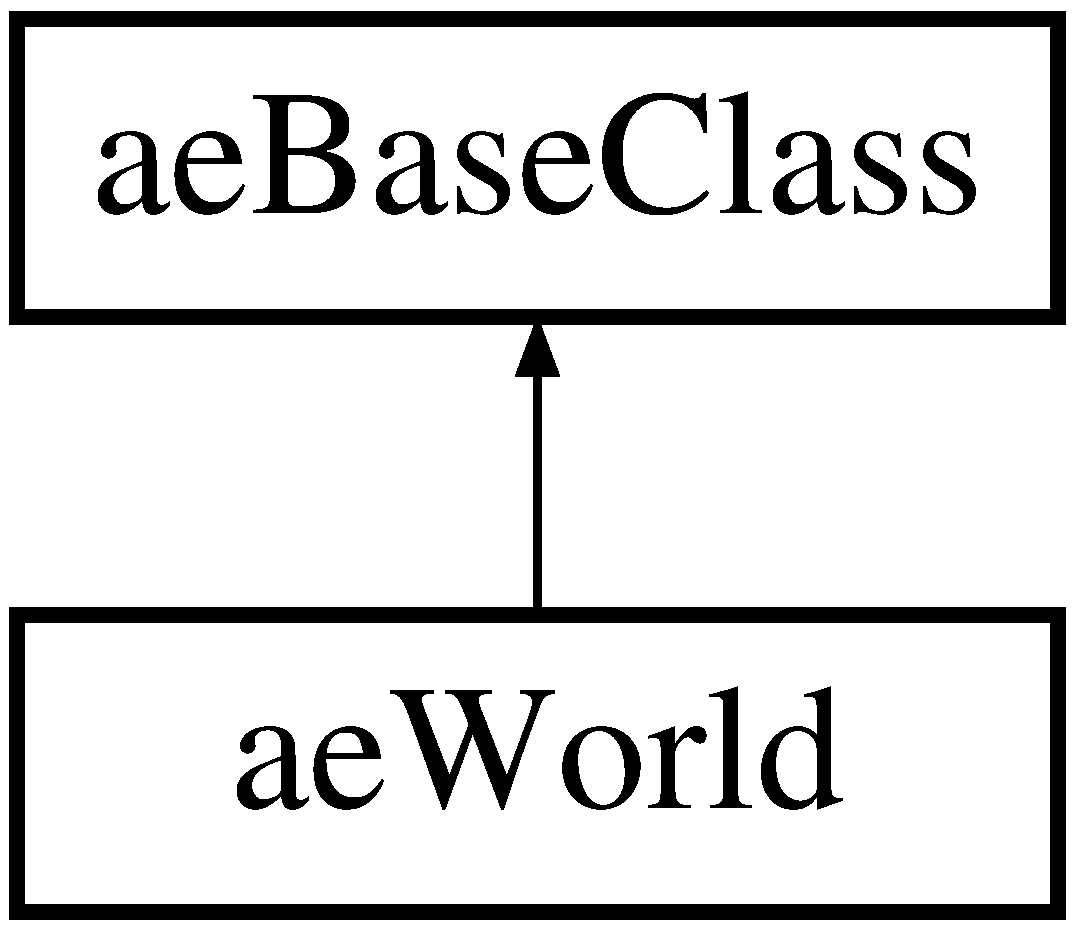
\includegraphics[height=2.000000cm]{classae_world}
\end{center}
\end{figure}
\subsection*{Public Member Functions}
\begin{DoxyCompactItemize}
\item 
int {\bfseries Init} (\hyperlink{namespaceae_core_ad6f85aacc0d1fdd85e458e2413e60010}{ae\+String} \&psz\+Bin\+File\+Path, \hyperlink{structae_core_1_1ae_rect}{ae\+Rect} Window\+Rect, \hyperlink{structae_core_1_1ae_rect}{ae\+Rect} World\+Render\+Rect, \hyperlink{classae_core_1_1ae_renderer}{ae\+Renderer} $\ast$p\+Renderer, \hyperlink{classae_core_1_1ae_clock}{ae\+Clock} $\ast$p\+Clock, Sprite\+List $\ast$p\+Sprites, Presets\+List $\ast$p\+Preset\+List)\hypertarget{classae_world_a0451a9905334a324deb1722d57dcc584}{}\label{classae_world_a0451a9905334a324deb1722d57dcc584}

\item 
void \hyperlink{classae_world_af3718f8cc66f64c7238c3b3d83987ae2}{Destroy} ()\hypertarget{classae_world_af3718f8cc66f64c7238c3b3d83987ae2}{}\label{classae_world_af3718f8cc66f64c7238c3b3d83987ae2}

\begin{DoxyCompactList}\small\item\em Destroys this object. \end{DoxyCompactList}\item 
void {\bfseries Update} (float f\+Delta)\hypertarget{classae_world_ae3c82e84e1e7246617bf11c387f11dc8}{}\label{classae_world_ae3c82e84e1e7246617bf11c387f11dc8}

\item 
void {\bfseries Render} (\hyperlink{classae_core_1_1ae_renderer}{ae\+Renderer} $\ast$p\+Renderer)\hypertarget{classae_world_a81ce74e0952df1c351dc65a8cc97be53}{}\label{classae_world_a81ce74e0952df1c351dc65a8cc97be53}

\item 
void {\bfseries Set\+Window\+Dimensions} (\hyperlink{structae_core_1_1ae_rect}{ae\+Rect} \&Window\+Rect, \hyperlink{structae_core_1_1ae_rect}{ae\+Rect} \&World\+Rect)\hypertarget{classae_world_a1a1b9f1dbb2375d10cda59e08be64db7}{}\label{classae_world_a1a1b9f1dbb2375d10cda59e08be64db7}

\item 
void {\bfseries Clic} (\hyperlink{structae_core_1_1ae_point}{ae\+Point} \&Clic\+Point, int Button)\hypertarget{classae_world_a0e0f8395684f11ee8d2271e32fd7f98e}{}\label{classae_world_a0e0f8395684f11ee8d2271e32fd7f98e}

\item 
void {\bfseries Cursor\+Update} (\hyperlink{structae_core_1_1ae_point}{ae\+Point} \&Cursor\+Position)\hypertarget{classae_world_abf8481b5949dea89bf90e7e65912c5ee}{}\label{classae_world_abf8481b5949dea89bf90e7e65912c5ee}

\item 
void {\bfseries Create\+Unit} (\hyperlink{namespaceae_core_ad6f85aacc0d1fdd85e458e2413e60010}{ae\+String} Unit\+Name, \hyperlink{structae_core_1_1ae_vector2}{ae\+Vector2} Position, \hyperlink{structae_core_1_1ae_vector2}{ae\+Vector2} Direction, int Team\+ID)\hypertarget{classae_world_abdc06894641a479b0c548b0f49171c26}{}\label{classae_world_abdc06894641a479b0c548b0f49171c26}

\item 
bool $\ast$ {\bfseries Is\+Isometric} ()\hypertarget{classae_world_a28dd44f8ee659c36795199717ca3b7d5}{}\label{classae_world_a28dd44f8ee659c36795199717ca3b7d5}

\item 
\hyperlink{structae_core_1_1ae_point}{ae\+Point} $\ast$ {\bfseries Get\+Size\+Of\+World} ()\hypertarget{classae_world_a716fdfed8742c0e704b7813241c25173}{}\label{classae_world_a716fdfed8742c0e704b7813241c25173}

\item 
\hyperlink{structae_core_1_1ae_rect}{ae\+Rect} $\ast$ {\bfseries Get\+Camera\+Rect} ()\hypertarget{classae_world_a18a9bad12e421cbd95b70a430dd09d4b}{}\label{classae_world_a18a9bad12e421cbd95b70a430dd09d4b}

\item 
\hyperlink{structae_core_1_1ae_vector2}{ae\+Vector2} $\ast$ {\bfseries Get\+Camera\+Position} ()\hypertarget{classae_world_a9316805d3c2bec56c144548dff1f4408}{}\label{classae_world_a9316805d3c2bec56c144548dff1f4408}

\item 
\hyperlink{class_c_animation}{C\+Animation} $\ast$ {\bfseries Get\+Animation} (int ID, int \hyperlink{_base_class_8h_aded8224779c70fab5084220935d672bba46a2a41cc6e552044816a2d04634545d}{State}, int Direction)\hypertarget{classae_world_a7fc2feb0c98ecaa1f2602a1fbc1d405a}{}\label{classae_world_a7fc2feb0c98ecaa1f2602a1fbc1d405a}

\end{DoxyCompactItemize}
\subsection*{Friends}
\begin{DoxyCompactItemize}
\item 
class {\bfseries ae\+G\+UI}\hypertarget{classae_world_ad62c7f93a3011eb3196872c9589382dd}{}\label{classae_world_ad62c7f93a3011eb3196872c9589382dd}

\end{DoxyCompactItemize}
\subsection*{Additional Inherited Members}


The documentation for this class was generated from the following files\+:\begin{DoxyCompactItemize}
\item 
C\+:/\+Users/\+Alvaro Estrada/\+Documents/\+Visual Studio 2015/\+Projects/\+R\+T\+S\+\_\+\+A\+E/\+R\+T\+S\+\_\+\+A\+E/\+Game/World.\+h\item 
C\+:/\+Users/\+Alvaro Estrada/\+Documents/\+Visual Studio 2015/\+Projects/\+R\+T\+S\+\_\+\+A\+E/\+R\+T\+S\+\_\+\+A\+E/\+Game/World.\+cpp\end{DoxyCompactItemize}

\hypertarget{class_c_animation}{}\section{C\+Animation Class Reference}
\label{class_c_animation}\index{C\+Animation@{C\+Animation}}
\subsection*{Public Member Functions}
\begin{DoxyCompactItemize}
\item 
{\bfseries C\+Animation} (\hyperlink{structae_core_1_1ae_rect}{ae\+Rect} $\ast$p\+Camera\+Rect, \hyperlink{structae_core_1_1ae_vector2}{ae\+Vector2} $\ast$p\+Camera\+Pos, bool $\ast$p\+Isometric)\hypertarget{class_c_animation_a529b032bfe42b5ed8aa11196c8e2502e}{}\label{class_c_animation_a529b032bfe42b5ed8aa11196c8e2502e}

\item 
void {\bfseries Delete} ()\hypertarget{class_c_animation_a55b661df0f9c47225e6d31ba9bed5343}{}\label{class_c_animation_a55b661df0f9c47225e6d31ba9bed5343}

\item 
void {\bfseries Play} ()\hypertarget{class_c_animation_ae42e8f48d0ef972df125f9e7f6af572a}{}\label{class_c_animation_ae42e8f48d0ef972df125f9e7f6af572a}

\item 
void {\bfseries Stop} ()\hypertarget{class_c_animation_a0825efd6c38498af6c3a73493c91d973}{}\label{class_c_animation_a0825efd6c38498af6c3a73493c91d973}

\item 
void {\bfseries Pause} ()\hypertarget{class_c_animation_ae3a125b48bc92e51c629674efc275155}{}\label{class_c_animation_ae3a125b48bc92e51c629674efc275155}

\item 
void {\bfseries Set} (float Current\+Time, \hyperlink{namespaceae_core_aa13093dc911869e5b24942552898f01f}{uint8} Booleans)\hypertarget{class_c_animation_ad39c8b208f8a11941a0c595480420a72}{}\label{class_c_animation_ad39c8b208f8a11941a0c595480420a72}

\item 
void {\bfseries Render} (\hyperlink{classae_core_1_1ae_renderer}{ae\+Renderer} $\ast$p\+Renderer, \hyperlink{structae_transform}{ae\+Transform} Upper\+Transform, float Current\+Time, bool MirrorX, \hyperlink{namespaceae_core_aa13093dc911869e5b24942552898f01f}{uint8} Booleans)\hypertarget{class_c_animation_a0e8b47609f48e3d6fb56bf0f7da9145e}{}\label{class_c_animation_a0e8b47609f48e3d6fb56bf0f7da9145e}

\item 
void {\bfseries Load\+Sprite} (\hyperlink{classae_core_1_1ae_sprite}{ae\+Sprite} $\ast$p\+Image)\hypertarget{class_c_animation_a1329eb2c481deacc9e54de79eed31835}{}\label{class_c_animation_a1329eb2c481deacc9e54de79eed31835}

\item 
void {\bfseries Insert\+Frame} (\hyperlink{structae_core_1_1ae_rect}{ae\+Rect} Source\+Rect, float Finish\+Time, bool MirrorX)\hypertarget{class_c_animation_a8d680ab84ed93b983edc1590a615ca1f}{}\label{class_c_animation_a8d680ab84ed93b983edc1590a615ca1f}

\item 
void {\bfseries Set\+Loop} ()\hypertarget{class_c_animation_a5eda2aff89757540e931c60bec234b73}{}\label{class_c_animation_a5eda2aff89757540e931c60bec234b73}

\end{DoxyCompactItemize}
\subsection*{Public Attributes}
\begin{DoxyCompactItemize}
\item 
bool {\bfseries MirrorX}\hypertarget{class_c_animation_ad0050c1a4dedaf1317e097b1c5c62729}{}\label{class_c_animation_ad0050c1a4dedaf1317e097b1c5c62729}

\item 
\hyperlink{structae_transform}{ae\+Transform} {\bfseries Transform}\hypertarget{class_c_animation_a931bd21d64556382f1cece9c509daa12}{}\label{class_c_animation_a931bd21d64556382f1cece9c509daa12}

\item 
bool {\bfseries m\+\_\+b\+Playing}\+: 1\hypertarget{class_c_animation_aa20f91f7b79a8c6fd98eec1c09723364}{}\label{class_c_animation_aa20f91f7b79a8c6fd98eec1c09723364}

\item 
bool {\bfseries m\+\_\+b\+Stopped}\+: 1\hypertarget{class_c_animation_a77f35dc5b97d414333c3c545660befa6}{}\label{class_c_animation_a77f35dc5b97d414333c3c545660befa6}

\item 
bool {\bfseries m\+\_\+b\+Paused}\+: 1\hypertarget{class_c_animation_a53b5f0e2f3065b8bfa42528a5ea6af77}{}\label{class_c_animation_a53b5f0e2f3065b8bfa42528a5ea6af77}

\item 
bool {\bfseries m\+\_\+b\+Ciclic}\+: 1\hypertarget{class_c_animation_a569a669fae8be99846b754d7b7232b1c}{}\label{class_c_animation_a569a669fae8be99846b754d7b7232b1c}

\item 
uint8 {\bfseries m\+\_\+byte\+Booleans}\hypertarget{class_c_animation_a9100d670c1feba6e8bd279a9067a675e}{}\label{class_c_animation_a9100d670c1feba6e8bd279a9067a675e}

\end{DoxyCompactItemize}


The documentation for this class was generated from the following files\+:\begin{DoxyCompactItemize}
\item 
C\+:/\+Users/\+Alvaro Estrada/\+Documents/\+Visual Studio 2015/\+Projects/\+R\+T\+S\+\_\+\+A\+E/\+R\+T\+S\+\_\+\+A\+E/\+Game/Animation.\+h\item 
C\+:/\+Users/\+Alvaro Estrada/\+Documents/\+Visual Studio 2015/\+Projects/\+R\+T\+S\+\_\+\+A\+E/\+R\+T\+S\+\_\+\+A\+E/\+Game/Animation.\+cpp\end{DoxyCompactItemize}

\hypertarget{class_c_animation_renderer}{}\section{C\+Animation\+Renderer Class Reference}
\label{class_c_animation_renderer}\index{C\+Animation\+Renderer@{C\+Animation\+Renderer}}
Inheritance diagram for C\+Animation\+Renderer\+:\begin{figure}[H]
\begin{center}
\leavevmode
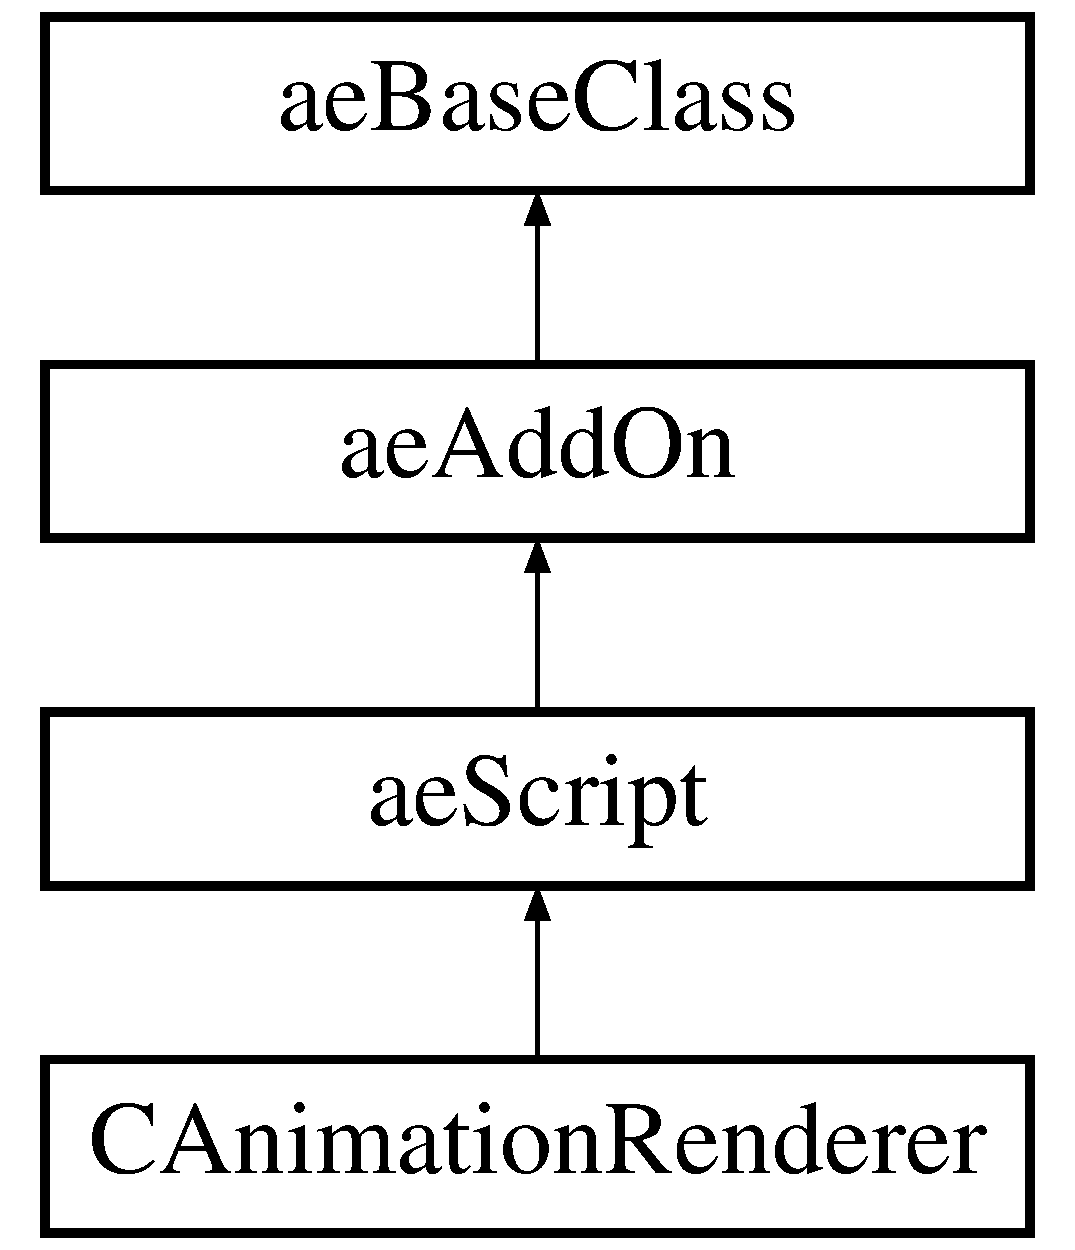
\includegraphics[height=4.000000cm]{class_c_animation_renderer}
\end{center}
\end{figure}
\subsection*{Public Member Functions}
\begin{DoxyCompactItemize}
\item 
virtual int \hyperlink{class_c_animation_renderer_abf2ab0201171989cf7ad44846cf3e115}{Init} (\hyperlink{classae_base_class}{ae\+Base\+Class} $\ast$p\+Parent)
\begin{DoxyCompactList}\small\item\em Initializes with the given parent pointer. \end{DoxyCompactList}\item 
virtual void \hyperlink{class_c_animation_renderer_a2ac2237cb706d2f6d45a88a86543e008}{Update} (float f\+Delta)
\begin{DoxyCompactList}\small\item\em Updates the given f\+Delta. \end{DoxyCompactList}\item 
virtual void \hyperlink{class_c_animation_renderer_a272f2bac72c90d89a9ada38058fc3f0c}{Render} (\hyperlink{classae_core_1_1ae_renderer}{ae\+Renderer} $\ast$p\+Renderer)
\begin{DoxyCompactList}\small\item\em Paints on the given renderer pointer. \end{DoxyCompactList}\item 
virtual void \hyperlink{class_c_animation_renderer_a4da67eb466b508135fe2ce38538f8ce0}{Destroy} ()\hypertarget{class_c_animation_renderer_a4da67eb466b508135fe2ce38538f8ce0}{}\label{class_c_animation_renderer_a4da67eb466b508135fe2ce38538f8ce0}

\begin{DoxyCompactList}\small\item\em Destroys this object. \end{DoxyCompactList}\item 
virtual void {\bfseries Set\+Object} (void $\ast$Object, bool Mirrorx)\hypertarget{class_c_animation_renderer_a62384e0a387b6aa37ce99448f7b07f4b}{}\label{class_c_animation_renderer_a62384e0a387b6aa37ce99448f7b07f4b}

\end{DoxyCompactItemize}
\subsection*{Public Attributes}
\begin{DoxyCompactItemize}
\item 
bool {\bfseries b\+Render}\hypertarget{class_c_animation_renderer_a3bb59d43ab8359500e5bd613cda99d50}{}\label{class_c_animation_renderer_a3bb59d43ab8359500e5bd613cda99d50}

\item 
uint8 {\bfseries Booleans}\hypertarget{class_c_animation_renderer_ab8ca07f77bb885dab14185ab31e6228e}{}\label{class_c_animation_renderer_ab8ca07f77bb885dab14185ab31e6228e}

\item 
float {\bfseries Current\+Time}\hypertarget{class_c_animation_renderer_ab36e10f877667f709d67d6f9d7bc9f11}{}\label{class_c_animation_renderer_ab36e10f877667f709d67d6f9d7bc9f11}

\item 
int {\bfseries Order\+Of\+Render}\hypertarget{class_c_animation_renderer_ab68b3daafdbbd9f33ec77b48384a7c00}{}\label{class_c_animation_renderer_ab68b3daafdbbd9f33ec77b48384a7c00}

\item 
bool {\bfseries MirrorX}\hypertarget{class_c_animation_renderer_a6417db8dcc583037136cc73c844817dd}{}\label{class_c_animation_renderer_a6417db8dcc583037136cc73c844817dd}

\item 
bool {\bfseries MirrorY}\hypertarget{class_c_animation_renderer_abbd0cd3acddcc7a3bfe38e2583ef30ca}{}\label{class_c_animation_renderer_abbd0cd3acddcc7a3bfe38e2583ef30ca}

\item 
ae\+Rect {\bfseries Render\+Rect}\hypertarget{class_c_animation_renderer_add36bcb728961d5f19254fe78eab7d50}{}\label{class_c_animation_renderer_add36bcb728961d5f19254fe78eab7d50}

\item 
ae\+Rect {\bfseries Source\+Rect}\hypertarget{class_c_animation_renderer_a167120445e1689108f12f6edcd2ed1c5}{}\label{class_c_animation_renderer_a167120445e1689108f12f6edcd2ed1c5}

\end{DoxyCompactItemize}
\subsection*{Additional Inherited Members}


\subsection{Member Function Documentation}
\index{C\+Animation\+Renderer@{C\+Animation\+Renderer}!Init@{Init}}
\index{Init@{Init}!C\+Animation\+Renderer@{C\+Animation\+Renderer}}
\subsubsection[{\texorpdfstring{Init(ae\+Base\+Class $\ast$p\+Parent)}{Init(aeBaseClass *pParent)}}]{\setlength{\rightskip}{0pt plus 5cm}int C\+Animation\+Renderer\+::\+Init (
\begin{DoxyParamCaption}
\item[{{\bf ae\+Base\+Class} $\ast$}]{p\+Parent}
\end{DoxyParamCaption}
)\hspace{0.3cm}{\ttfamily [virtual]}}\hypertarget{class_c_animation_renderer_abf2ab0201171989cf7ad44846cf3e115}{}\label{class_c_animation_renderer_abf2ab0201171989cf7ad44846cf3e115}


Initializes with the given parent pointer. 


\begin{DoxyParams}[1]{Parameters}
\mbox{\tt in,out}  & {\em p\+Parent} & If non-\/null, the parent pointer. \\
\hline
\end{DoxyParams}


Implements \hyperlink{classae_add_on_a0730c1446e548031f9a4e98435a54675}{ae\+Add\+On}.

\index{C\+Animation\+Renderer@{C\+Animation\+Renderer}!Render@{Render}}
\index{Render@{Render}!C\+Animation\+Renderer@{C\+Animation\+Renderer}}
\subsubsection[{\texorpdfstring{Render(ae\+Renderer $\ast$p\+Renderer)}{Render(aeRenderer *pRenderer)}}]{\setlength{\rightskip}{0pt plus 5cm}void C\+Animation\+Renderer\+::\+Render (
\begin{DoxyParamCaption}
\item[{{\bf ae\+Renderer} $\ast$}]{p\+Renderer}
\end{DoxyParamCaption}
)\hspace{0.3cm}{\ttfamily [virtual]}}\hypertarget{class_c_animation_renderer_a272f2bac72c90d89a9ada38058fc3f0c}{}\label{class_c_animation_renderer_a272f2bac72c90d89a9ada38058fc3f0c}


Paints on the given renderer pointer. 


\begin{DoxyParams}[1]{Parameters}
\mbox{\tt in,out}  & {\em p\+Renderer} & The renderer pointer. \\
\hline
\end{DoxyParams}


Reimplemented from \hyperlink{classae_add_on_ab6bed56009b9c92df8ae017a27587dc3}{ae\+Add\+On}.

\index{C\+Animation\+Renderer@{C\+Animation\+Renderer}!Update@{Update}}
\index{Update@{Update}!C\+Animation\+Renderer@{C\+Animation\+Renderer}}
\subsubsection[{\texorpdfstring{Update(float f\+Delta)}{Update(float fDelta)}}]{\setlength{\rightskip}{0pt plus 5cm}void C\+Animation\+Renderer\+::\+Update (
\begin{DoxyParamCaption}
\item[{float}]{f\+Delta}
\end{DoxyParamCaption}
)\hspace{0.3cm}{\ttfamily [virtual]}}\hypertarget{class_c_animation_renderer_a2ac2237cb706d2f6d45a88a86543e008}{}\label{class_c_animation_renderer_a2ac2237cb706d2f6d45a88a86543e008}


Updates the given f\+Delta. 


\begin{DoxyParams}{Parameters}
{\em f\+Delta} & The delta time. \\
\hline
\end{DoxyParams}


Implements \hyperlink{classae_add_on_a51caa4b8680206495ea671e71991e231}{ae\+Add\+On}.



The documentation for this class was generated from the following files\+:\begin{DoxyCompactItemize}
\item 
C\+:/\+Users/\+Alvaro Estrada/\+Documents/\+Visual Studio 2015/\+Projects/\+R\+T\+S\+\_\+\+A\+E/\+R\+T\+S\+\_\+\+A\+E/\+Game/Animation\+Renderer.\+h\item 
C\+:/\+Users/\+Alvaro Estrada/\+Documents/\+Visual Studio 2015/\+Projects/\+R\+T\+S\+\_\+\+A\+E/\+R\+T\+S\+\_\+\+A\+E/\+Game/Animation\+Renderer.\+cpp\end{DoxyCompactItemize}

\hypertarget{class_c_animation_state}{}\section{C\+Animation\+State Class Reference}
\label{class_c_animation_state}\index{C\+Animation\+State@{C\+Animation\+State}}
Inheritance diagram for C\+Animation\+State\+:\begin{figure}[H]
\begin{center}
\leavevmode
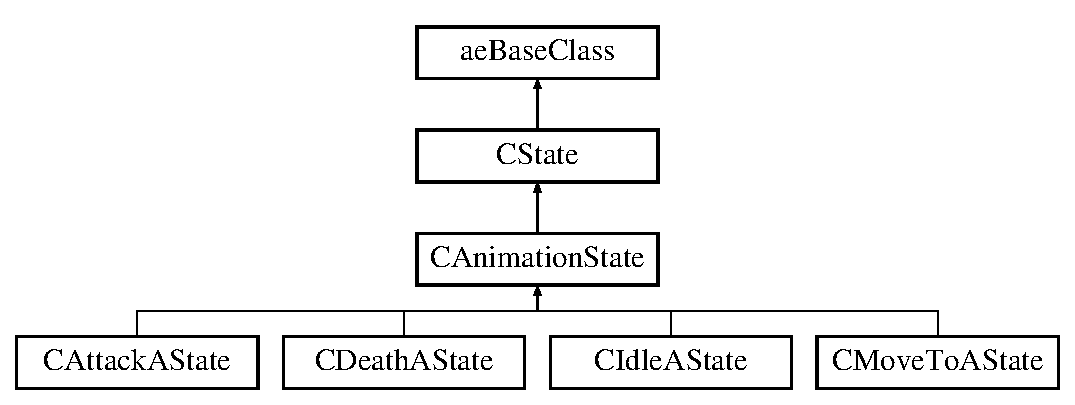
\includegraphics[height=4.000000cm]{class_c_animation_state}
\end{center}
\end{figure}
\subsection*{Public Member Functions}
\begin{DoxyCompactItemize}
\item 
void {\bfseries Set\+World\+Reference} (\hyperlink{classae_world}{ae\+World} $\ast$p\+World\+Reference)\hypertarget{class_c_animation_state_a09ff62a475a6bcca566a81d4026e4940}{}\label{class_c_animation_state_a09ff62a475a6bcca566a81d4026e4940}

\end{DoxyCompactItemize}
\subsection*{Protected Attributes}
\begin{DoxyCompactItemize}
\item 
\begin{tabbing}
xx\=xx\=xx\=xx\=xx\=xx\=xx\=xx\=xx\=\kill
union \{\\
\>struct \{\\
\>\>bool {\bfseries m\_bPlaying}: 1\\
\>\>bool {\bfseries m\_bStopped}: 1\\
\>\>bool {\bfseries m\_bPaused}: 1\\
\>\>bool {\bfseries m\_bCiclic}: 1\\
\>\} \hypertarget{union_c_animation_state_1_1_0D38_af9375fe96e6af426dc09a76be22b1598}{}\label{union_c_animation_state_1_1_0D38_af9375fe96e6af426dc09a76be22b1598}
\\
\>uint8 {\bfseries m\_byteBooleans}\\
\}; \hypertarget{class_c_animation_state_a208eb30915b0beb4ec4322de36fc6b00}{}\label{class_c_animation_state_a208eb30915b0beb4ec4322de36fc6b00}
\\

\end{tabbing}\item 
\hyperlink{classae_world}{ae\+World} $\ast$ {\bfseries m\+\_\+p\+World\+Reference}\hypertarget{class_c_animation_state_aae2eaab07301fba6a3e8e441b5ccc905}{}\label{class_c_animation_state_aae2eaab07301fba6a3e8e441b5ccc905}

\end{DoxyCompactItemize}


The documentation for this class was generated from the following files\+:\begin{DoxyCompactItemize}
\item 
C\+:/\+Users/\+Alvaro Estrada/\+Documents/\+Visual Studio 2015/\+Projects/\+R\+T\+S\+\_\+\+A\+E/\+R\+T\+S\+\_\+\+A\+E/\+Game/Animation\+State.\+h\item 
C\+:/\+Users/\+Alvaro Estrada/\+Documents/\+Visual Studio 2015/\+Projects/\+R\+T\+S\+\_\+\+A\+E/\+R\+T\+S\+\_\+\+A\+E/\+Game/Animation\+State.\+cpp\end{DoxyCompactItemize}

\hypertarget{class_c_animation_state_machine}{}\section{C\+Animation\+State\+Machine Class Reference}
\label{class_c_animation_state_machine}\index{C\+Animation\+State\+Machine@{C\+Animation\+State\+Machine}}
Inheritance diagram for C\+Animation\+State\+Machine\+:\begin{figure}[H]
\begin{center}
\leavevmode
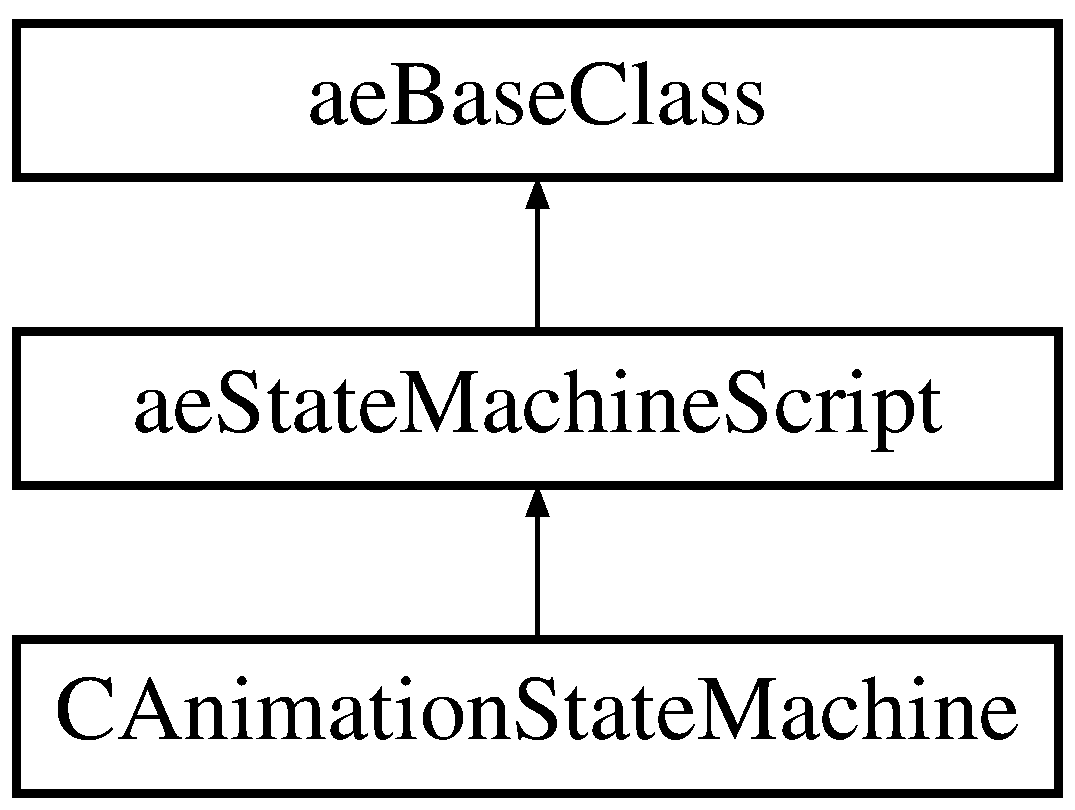
\includegraphics[height=3.000000cm]{class_c_animation_state_machine}
\end{center}
\end{figure}
\subsection*{Public Member Functions}
\begin{DoxyCompactItemize}
\item 
virtual void {\bfseries Set\+State} (int New\+State)\hypertarget{class_c_animation_state_machine_a5292c07ee3336f9ce812530ba2e9af45}{}\label{class_c_animation_state_machine_a5292c07ee3336f9ce812530ba2e9af45}

\end{DoxyCompactItemize}
\subsection*{Public Attributes}
\begin{DoxyCompactItemize}
\item 
void $\ast$ {\bfseries p\+Pass\+Along}\hypertarget{class_c_animation_state_machine_a010a4f14ebd53dfb297dee39e570c188}{}\label{class_c_animation_state_machine_a010a4f14ebd53dfb297dee39e570c188}

\end{DoxyCompactItemize}
\subsection*{Additional Inherited Members}


The documentation for this class was generated from the following files\+:\begin{DoxyCompactItemize}
\item 
C\+:/\+Users/\+Alvaro Estrada/\+Documents/\+Visual Studio 2015/\+Projects/\+R\+T\+S\+\_\+\+A\+E/\+R\+T\+S\+\_\+\+A\+E/\+Game/Animation\+State\+Machine.\+h\item 
C\+:/\+Users/\+Alvaro Estrada/\+Documents/\+Visual Studio 2015/\+Projects/\+R\+T\+S\+\_\+\+A\+E/\+R\+T\+S\+\_\+\+A\+E/\+Game/Animation\+State\+Machine.\+cpp\end{DoxyCompactItemize}

\hypertarget{class_c_attack}{}\section{C\+Attack Class Reference}
\label{class_c_attack}\index{C\+Attack@{C\+Attack}}
Inheritance diagram for C\+Attack\+:\begin{figure}[H]
\begin{center}
\leavevmode
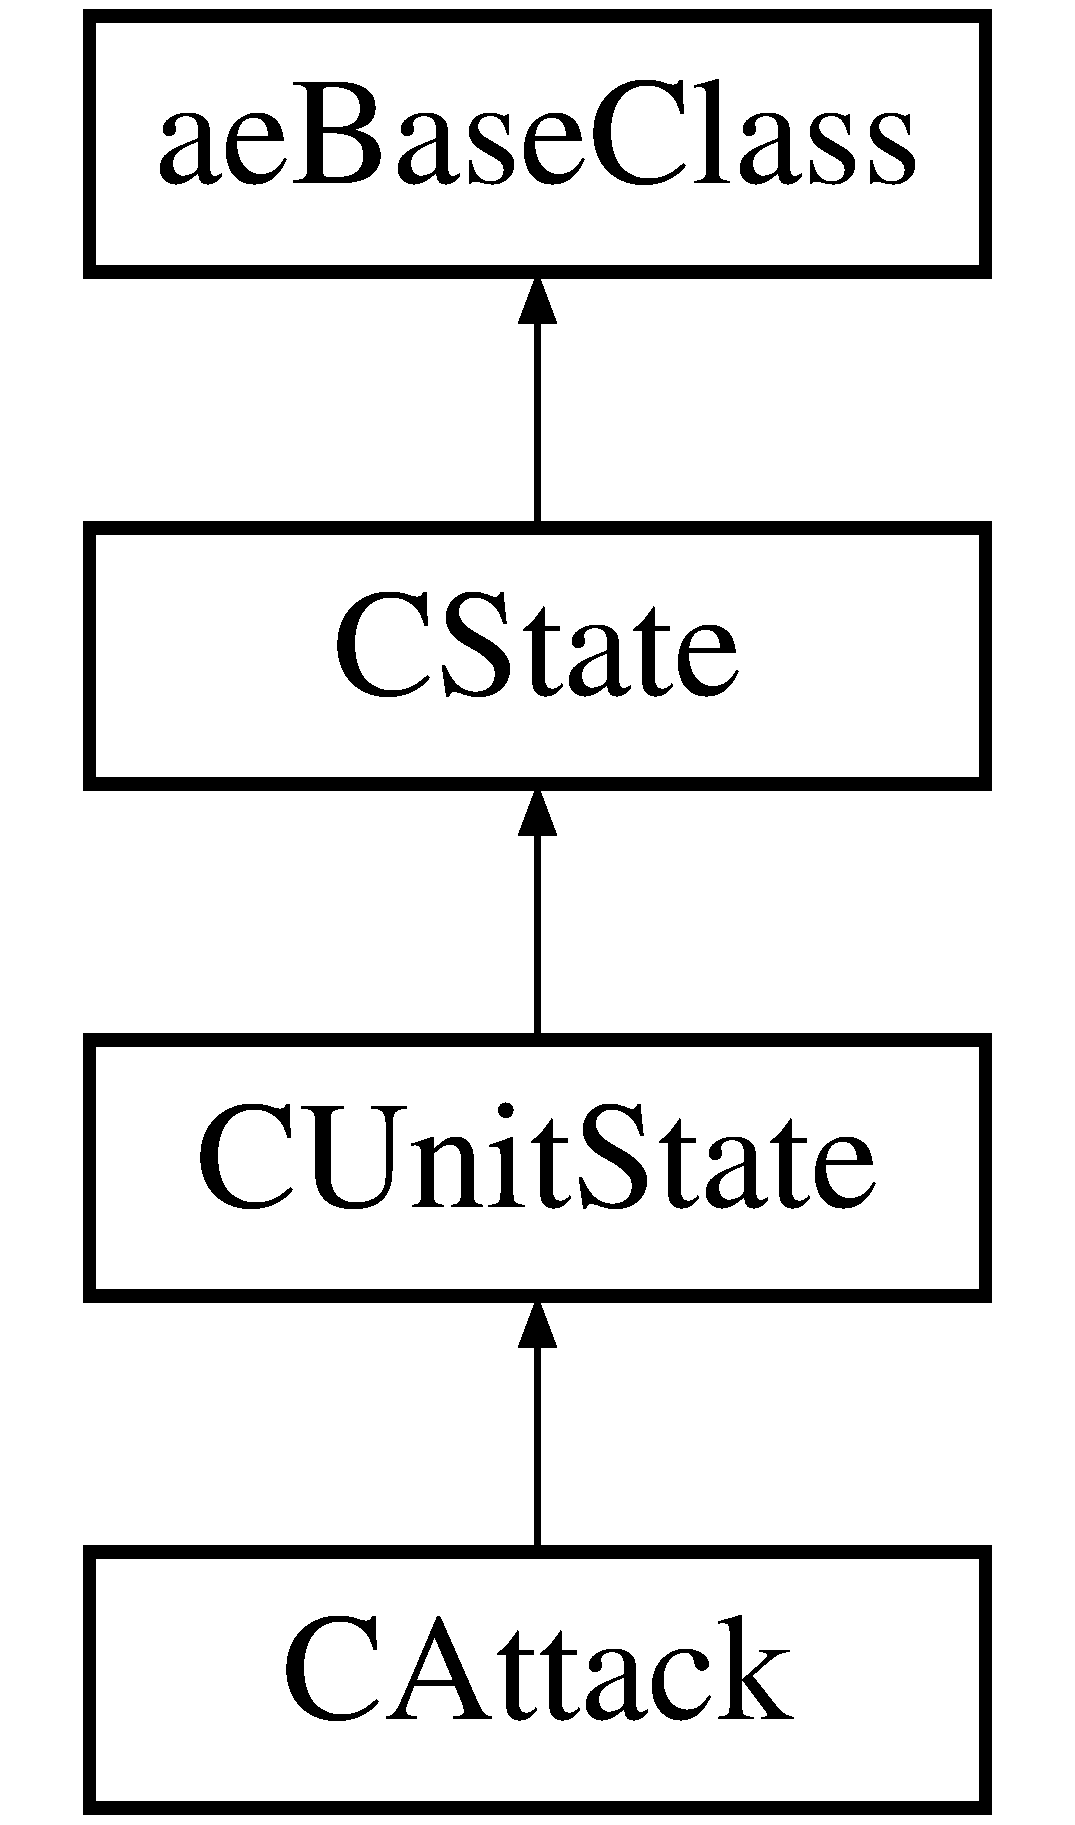
\includegraphics[height=4.000000cm]{class_c_attack}
\end{center}
\end{figure}
\subsection*{Public Member Functions}
\begin{DoxyCompactItemize}
\item 
virtual void \hyperlink{class_c_attack_ab01b39ae23ea81ebff5c8373cbec4908}{Init} (\hyperlink{classae_state_machine_script}{ae\+State\+Machine\+Script} $\ast$p\+Script)
\begin{DoxyCompactList}\small\item\em Initializes the with the given state machine script. \end{DoxyCompactList}\item 
virtual void \hyperlink{class_c_attack_a86bd55b2f6dfe8e046d7aa8c576c30b4}{Destroy} ()\hypertarget{class_c_attack_a86bd55b2f6dfe8e046d7aa8c576c30b4}{}\label{class_c_attack_a86bd55b2f6dfe8e046d7aa8c576c30b4}

\begin{DoxyCompactList}\small\item\em Destroys this object. \end{DoxyCompactList}\item 
virtual int \hyperlink{class_c_attack_a31becaa6458236fc037b022896dea8d2}{On\+Update} (float f\+Delta, \hyperlink{classae_base_class}{ae\+Base\+Class} $\ast$p\+Object)
\begin{DoxyCompactList}\small\item\em Executes the update action. \end{DoxyCompactList}\item 
virtual void \hyperlink{class_c_attack_ab859dd5a730ec7236e5dfa3e81cb40a8}{On\+Enter} ()\hypertarget{class_c_attack_ab859dd5a730ec7236e5dfa3e81cb40a8}{}\label{class_c_attack_ab859dd5a730ec7236e5dfa3e81cb40a8}

\begin{DoxyCompactList}\small\item\em Executes the enter action. \end{DoxyCompactList}\item 
virtual void \hyperlink{class_c_attack_a3670594a1dc95e94cfe0795c9804187e}{On\+Exit} ()\hypertarget{class_c_attack_a3670594a1dc95e94cfe0795c9804187e}{}\label{class_c_attack_a3670594a1dc95e94cfe0795c9804187e}

\begin{DoxyCompactList}\small\item\em Executes the exit action. \end{DoxyCompactList}\end{DoxyCompactItemize}
\subsection*{Additional Inherited Members}


\subsection{Member Function Documentation}
\index{C\+Attack@{C\+Attack}!Init@{Init}}
\index{Init@{Init}!C\+Attack@{C\+Attack}}
\subsubsection[{\texorpdfstring{Init(ae\+State\+Machine\+Script $\ast$p\+Script)}{Init(aeStateMachineScript *pScript)}}]{\setlength{\rightskip}{0pt plus 5cm}void C\+Attack\+::\+Init (
\begin{DoxyParamCaption}
\item[{{\bf ae\+State\+Machine\+Script} $\ast$}]{p\+Script}
\end{DoxyParamCaption}
)\hspace{0.3cm}{\ttfamily [virtual]}}\hypertarget{class_c_attack_ab01b39ae23ea81ebff5c8373cbec4908}{}\label{class_c_attack_ab01b39ae23ea81ebff5c8373cbec4908}


Initializes the with the given state machine script. 


\begin{DoxyParams}[1]{Parameters}
\mbox{\tt in,out}  & {\em p\+Script} & If non-\/null, the script. \\
\hline
\end{DoxyParams}


Implements \hyperlink{class_c_state_a220fab97e545680a7237dbb0d04ba037}{C\+State}.

\index{C\+Attack@{C\+Attack}!On\+Update@{On\+Update}}
\index{On\+Update@{On\+Update}!C\+Attack@{C\+Attack}}
\subsubsection[{\texorpdfstring{On\+Update(float f\+Delta, ae\+Base\+Class $\ast$p\+Object)}{OnUpdate(float fDelta, aeBaseClass *pObject)}}]{\setlength{\rightskip}{0pt plus 5cm}int C\+Attack\+::\+On\+Update (
\begin{DoxyParamCaption}
\item[{float}]{f\+Delta, }
\item[{{\bf ae\+Base\+Class} $\ast$}]{p\+Object}
\end{DoxyParamCaption}
)\hspace{0.3cm}{\ttfamily [virtual]}}\hypertarget{class_c_attack_a31becaa6458236fc037b022896dea8d2}{}\label{class_c_attack_a31becaa6458236fc037b022896dea8d2}


Executes the update action. 


\begin{DoxyParams}[1]{Parameters}
 & {\em f\+Delta} & The delta. \\
\hline
\mbox{\tt in,out}  & {\em p\+Object} & If non-\/null, the object.\\
\hline
\end{DoxyParams}
\begin{DoxyReturn}{Returns}
An int. 
\end{DoxyReturn}


Implements \hyperlink{class_c_state_a9d687e06b17b821703332fa3d4ea8bcf}{C\+State}.



The documentation for this class was generated from the following files\+:\begin{DoxyCompactItemize}
\item 
C\+:/\+Users/\+Alvaro Estrada/\+Documents/\+Visual Studio 2015/\+Projects/\+R\+T\+S\+\_\+\+A\+E/\+R\+T\+S\+\_\+\+A\+E/\+Game/Attack.\+h\item 
C\+:/\+Users/\+Alvaro Estrada/\+Documents/\+Visual Studio 2015/\+Projects/\+R\+T\+S\+\_\+\+A\+E/\+R\+T\+S\+\_\+\+A\+E/\+Game/Attack.\+cpp\end{DoxyCompactItemize}

\hypertarget{class_c_attack_a_state}{}\section{C\+Attack\+A\+State Class Reference}
\label{class_c_attack_a_state}\index{C\+Attack\+A\+State@{C\+Attack\+A\+State}}
Inheritance diagram for C\+Attack\+A\+State\+:\begin{figure}[H]
\begin{center}
\leavevmode
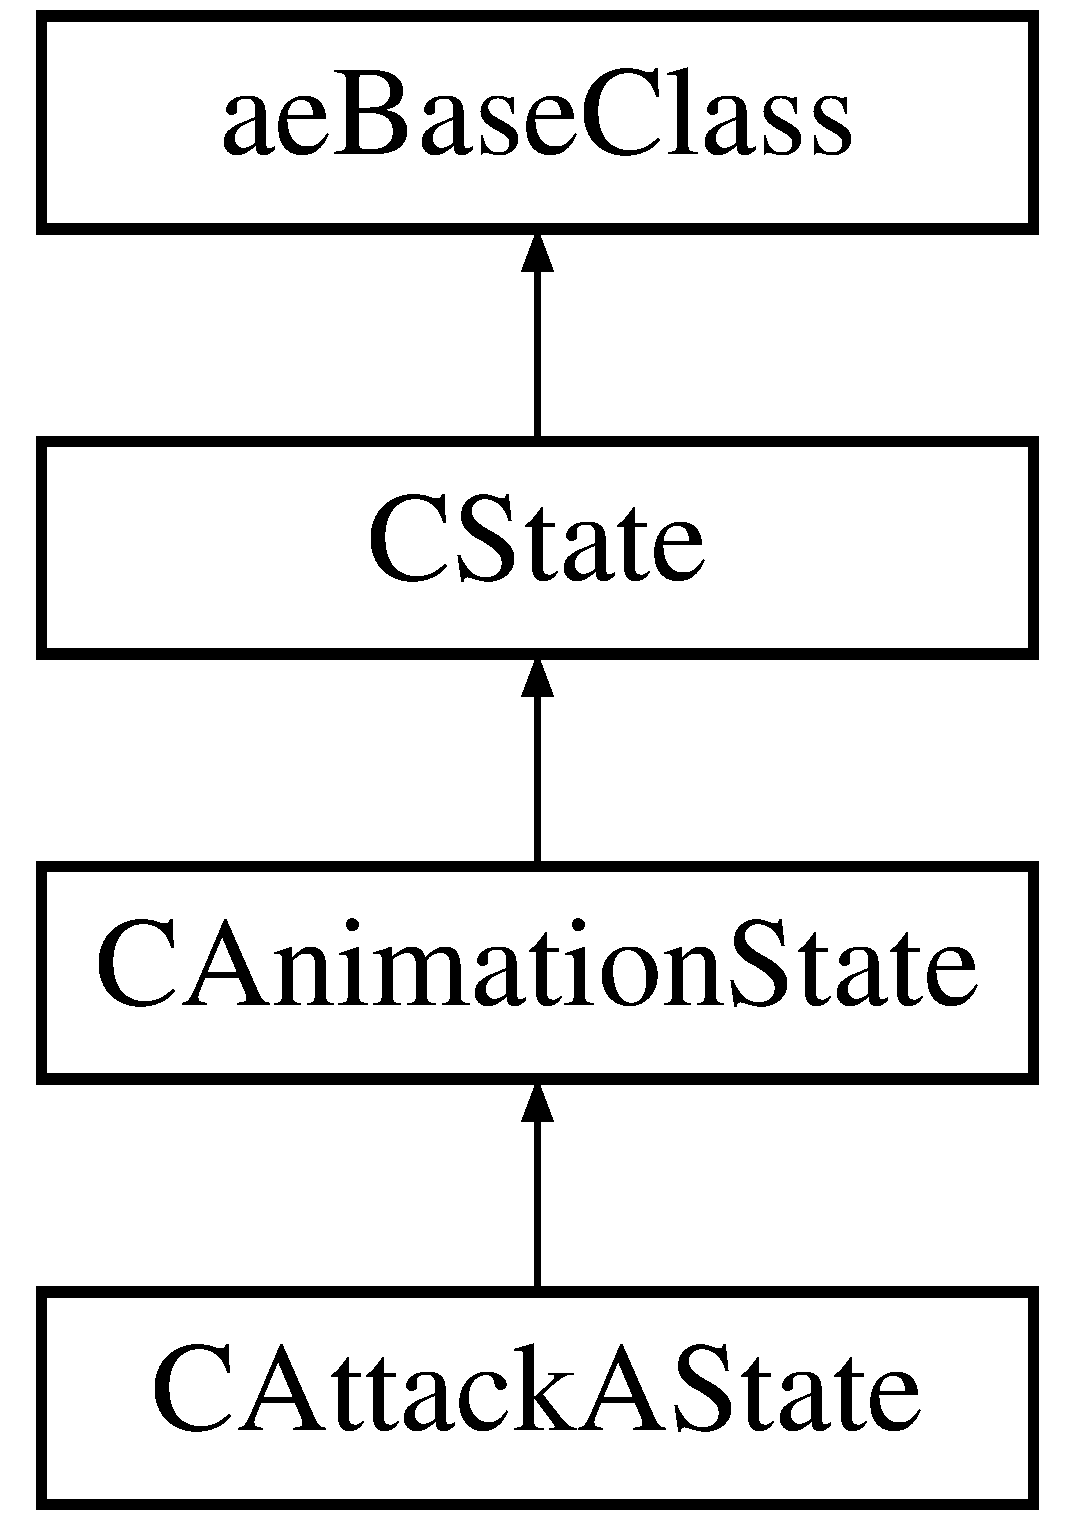
\includegraphics[height=4.000000cm]{class_c_attack_a_state}
\end{center}
\end{figure}
\subsection*{Public Member Functions}
\begin{DoxyCompactItemize}
\item 
virtual void \hyperlink{class_c_attack_a_state_aed0917a7321472f3b1756236355dfc9a}{Init} (\hyperlink{classae_state_machine_script}{ae\+State\+Machine\+Script} $\ast$p\+Script)
\begin{DoxyCompactList}\small\item\em Initializes the with the given state machine script. \end{DoxyCompactList}\item 
virtual void \hyperlink{class_c_attack_a_state_a585e3aca36d7303d16fc93233ee161ae}{Destroy} ()\hypertarget{class_c_attack_a_state_a585e3aca36d7303d16fc93233ee161ae}{}\label{class_c_attack_a_state_a585e3aca36d7303d16fc93233ee161ae}

\begin{DoxyCompactList}\small\item\em Destroys this object. \end{DoxyCompactList}\item 
virtual int \hyperlink{class_c_attack_a_state_adf86654143ca6f2fb44b1a2ea7346123}{On\+Update} (float f\+Delta, \hyperlink{classae_base_class}{ae\+Base\+Class} $\ast$p\+Object)
\begin{DoxyCompactList}\small\item\em Executes the update action. \end{DoxyCompactList}\item 
virtual void \hyperlink{class_c_attack_a_state_a6da54427c9209237cd9fc0ff5f1ef444}{On\+Enter} ()\hypertarget{class_c_attack_a_state_a6da54427c9209237cd9fc0ff5f1ef444}{}\label{class_c_attack_a_state_a6da54427c9209237cd9fc0ff5f1ef444}

\begin{DoxyCompactList}\small\item\em Executes the enter action. \end{DoxyCompactList}\item 
virtual void \hyperlink{class_c_attack_a_state_a58ee3ef13a5670330087475cf7a5149d}{On\+Exit} ()\hypertarget{class_c_attack_a_state_a58ee3ef13a5670330087475cf7a5149d}{}\label{class_c_attack_a_state_a58ee3ef13a5670330087475cf7a5149d}

\begin{DoxyCompactList}\small\item\em Executes the exit action. \end{DoxyCompactList}\end{DoxyCompactItemize}
\subsection*{Additional Inherited Members}


\subsection{Member Function Documentation}
\index{C\+Attack\+A\+State@{C\+Attack\+A\+State}!Init@{Init}}
\index{Init@{Init}!C\+Attack\+A\+State@{C\+Attack\+A\+State}}
\subsubsection[{\texorpdfstring{Init(ae\+State\+Machine\+Script $\ast$p\+Script)}{Init(aeStateMachineScript *pScript)}}]{\setlength{\rightskip}{0pt plus 5cm}void C\+Attack\+A\+State\+::\+Init (
\begin{DoxyParamCaption}
\item[{{\bf ae\+State\+Machine\+Script} $\ast$}]{p\+Script}
\end{DoxyParamCaption}
)\hspace{0.3cm}{\ttfamily [virtual]}}\hypertarget{class_c_attack_a_state_aed0917a7321472f3b1756236355dfc9a}{}\label{class_c_attack_a_state_aed0917a7321472f3b1756236355dfc9a}


Initializes the with the given state machine script. 


\begin{DoxyParams}[1]{Parameters}
\mbox{\tt in,out}  & {\em p\+Script} & If non-\/null, the script. \\
\hline
\end{DoxyParams}


Implements \hyperlink{class_c_state_a220fab97e545680a7237dbb0d04ba037}{C\+State}.

\index{C\+Attack\+A\+State@{C\+Attack\+A\+State}!On\+Update@{On\+Update}}
\index{On\+Update@{On\+Update}!C\+Attack\+A\+State@{C\+Attack\+A\+State}}
\subsubsection[{\texorpdfstring{On\+Update(float f\+Delta, ae\+Base\+Class $\ast$p\+Object)}{OnUpdate(float fDelta, aeBaseClass *pObject)}}]{\setlength{\rightskip}{0pt plus 5cm}int C\+Attack\+A\+State\+::\+On\+Update (
\begin{DoxyParamCaption}
\item[{float}]{f\+Delta, }
\item[{{\bf ae\+Base\+Class} $\ast$}]{p\+Object}
\end{DoxyParamCaption}
)\hspace{0.3cm}{\ttfamily [virtual]}}\hypertarget{class_c_attack_a_state_adf86654143ca6f2fb44b1a2ea7346123}{}\label{class_c_attack_a_state_adf86654143ca6f2fb44b1a2ea7346123}


Executes the update action. 


\begin{DoxyParams}[1]{Parameters}
 & {\em f\+Delta} & The delta. \\
\hline
\mbox{\tt in,out}  & {\em p\+Object} & If non-\/null, the object.\\
\hline
\end{DoxyParams}
\begin{DoxyReturn}{Returns}
An int. 
\end{DoxyReturn}


Implements \hyperlink{class_c_state_a9d687e06b17b821703332fa3d4ea8bcf}{C\+State}.



The documentation for this class was generated from the following files\+:\begin{DoxyCompactItemize}
\item 
C\+:/\+Users/\+Alvaro Estrada/\+Documents/\+Visual Studio 2015/\+Projects/\+R\+T\+S\+\_\+\+A\+E/\+R\+T\+S\+\_\+\+A\+E/\+Game/Attack\+A\+State.\+h\item 
C\+:/\+Users/\+Alvaro Estrada/\+Documents/\+Visual Studio 2015/\+Projects/\+R\+T\+S\+\_\+\+A\+E/\+R\+T\+S\+\_\+\+A\+E/\+Game/Attack\+A\+State.\+cpp\end{DoxyCompactItemize}

\hypertarget{class_c_death}{}\section{C\+Death Class Reference}
\label{class_c_death}\index{C\+Death@{C\+Death}}
Inheritance diagram for C\+Death\+:\begin{figure}[H]
\begin{center}
\leavevmode
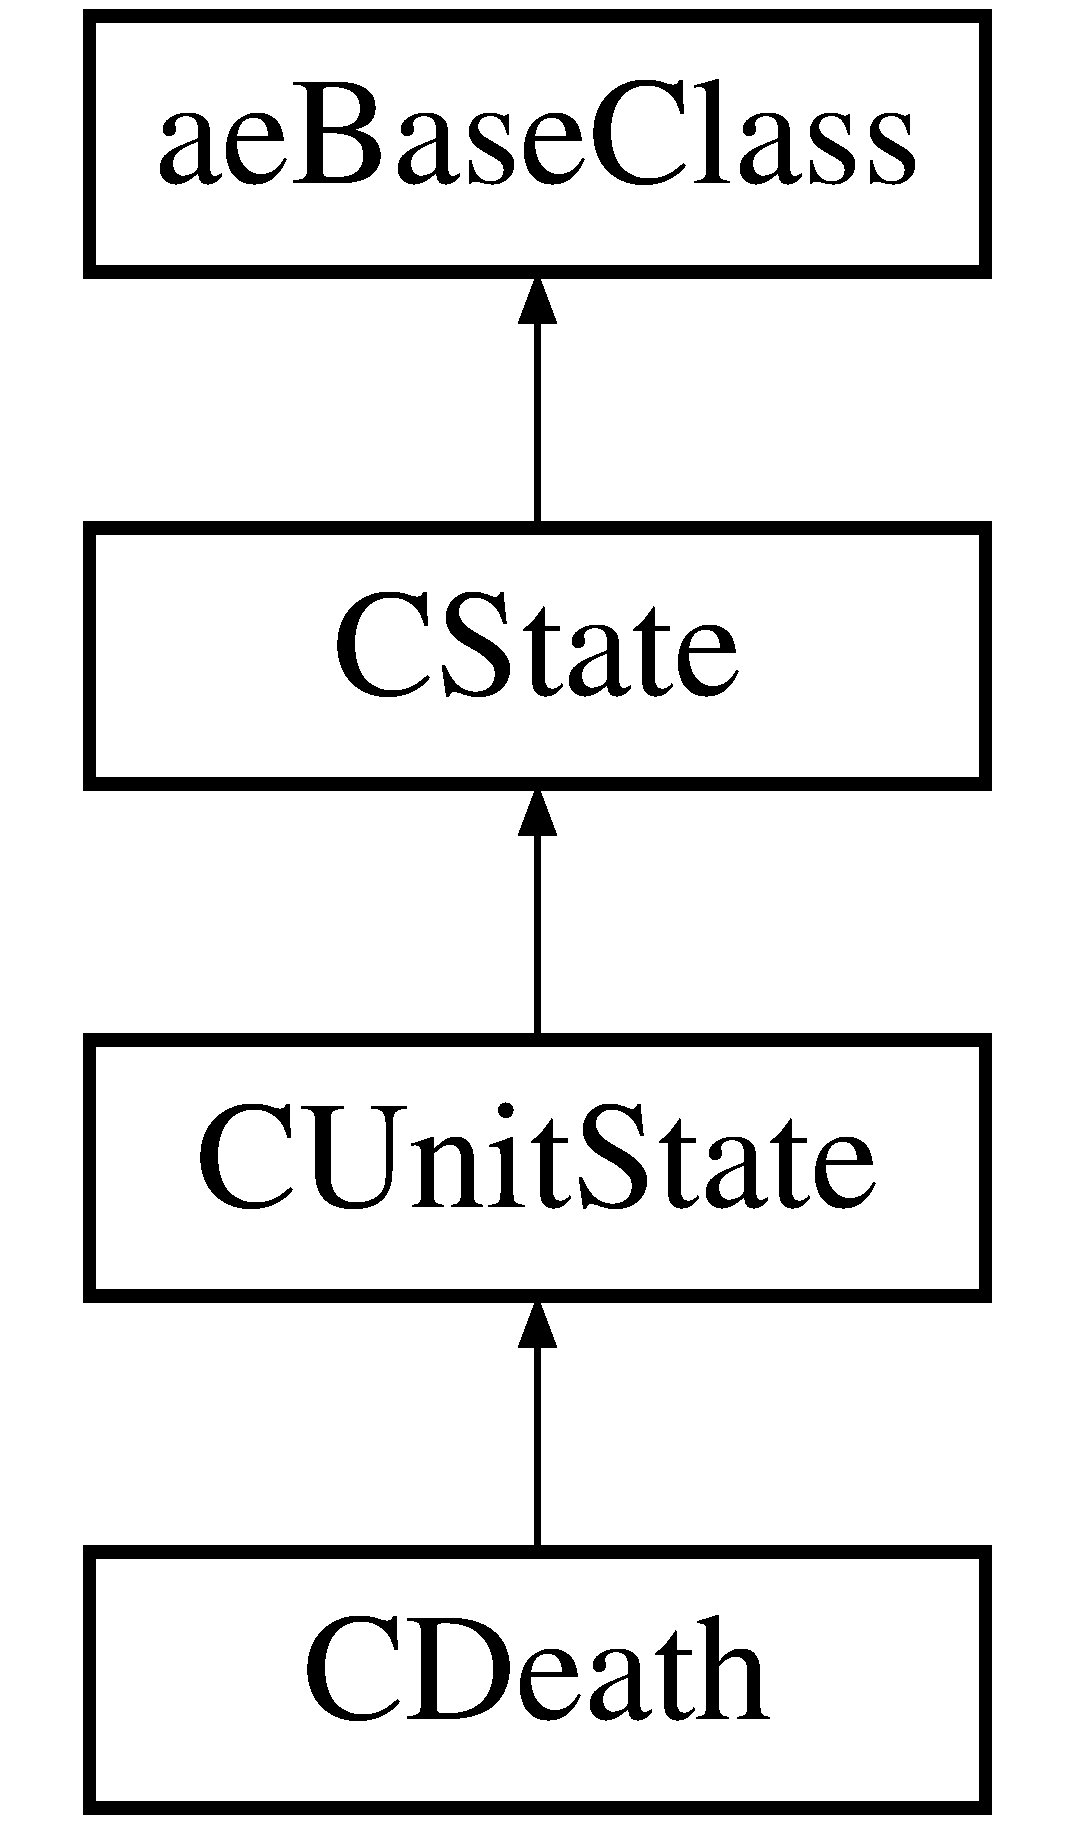
\includegraphics[height=4.000000cm]{class_c_death}
\end{center}
\end{figure}
\subsection*{Public Member Functions}
\begin{DoxyCompactItemize}
\item 
virtual void \hyperlink{class_c_death_a3cabf498e0212ec61fe3575a75cc72ca}{Init} (\hyperlink{classae_state_machine_script}{ae\+State\+Machine\+Script} $\ast$p\+Script)
\begin{DoxyCompactList}\small\item\em Initializes the with the given state machine script. \end{DoxyCompactList}\item 
virtual void \hyperlink{class_c_death_a7701d6ff70e21f5592699c3195119a7d}{Destroy} ()\hypertarget{class_c_death_a7701d6ff70e21f5592699c3195119a7d}{}\label{class_c_death_a7701d6ff70e21f5592699c3195119a7d}

\begin{DoxyCompactList}\small\item\em Destroys this object. \end{DoxyCompactList}\item 
virtual int \hyperlink{class_c_death_a23bc4e0cc320b368cf103547532ffee9}{On\+Update} (float f\+Delta, \hyperlink{classae_base_class}{ae\+Base\+Class} $\ast$p\+Object)
\begin{DoxyCompactList}\small\item\em Executes the update action. \end{DoxyCompactList}\item 
virtual void \hyperlink{class_c_death_afa81b21b56e0a445e9b9c377100aa350}{On\+Enter} ()\hypertarget{class_c_death_afa81b21b56e0a445e9b9c377100aa350}{}\label{class_c_death_afa81b21b56e0a445e9b9c377100aa350}

\begin{DoxyCompactList}\small\item\em Executes the enter action. \end{DoxyCompactList}\item 
virtual void \hyperlink{class_c_death_a03ae29a31707fefb92378e53e9b87c9a}{On\+Exit} ()\hypertarget{class_c_death_a03ae29a31707fefb92378e53e9b87c9a}{}\label{class_c_death_a03ae29a31707fefb92378e53e9b87c9a}

\begin{DoxyCompactList}\small\item\em Executes the exit action. \end{DoxyCompactList}\end{DoxyCompactItemize}
\subsection*{Additional Inherited Members}


\subsection{Member Function Documentation}
\index{C\+Death@{C\+Death}!Init@{Init}}
\index{Init@{Init}!C\+Death@{C\+Death}}
\subsubsection[{\texorpdfstring{Init(ae\+State\+Machine\+Script $\ast$p\+Script)}{Init(aeStateMachineScript *pScript)}}]{\setlength{\rightskip}{0pt plus 5cm}void C\+Death\+::\+Init (
\begin{DoxyParamCaption}
\item[{{\bf ae\+State\+Machine\+Script} $\ast$}]{p\+Script}
\end{DoxyParamCaption}
)\hspace{0.3cm}{\ttfamily [virtual]}}\hypertarget{class_c_death_a3cabf498e0212ec61fe3575a75cc72ca}{}\label{class_c_death_a3cabf498e0212ec61fe3575a75cc72ca}


Initializes the with the given state machine script. 


\begin{DoxyParams}[1]{Parameters}
\mbox{\tt in,out}  & {\em p\+Script} & If non-\/null, the script. \\
\hline
\end{DoxyParams}


Implements \hyperlink{class_c_state_a220fab97e545680a7237dbb0d04ba037}{C\+State}.

\index{C\+Death@{C\+Death}!On\+Update@{On\+Update}}
\index{On\+Update@{On\+Update}!C\+Death@{C\+Death}}
\subsubsection[{\texorpdfstring{On\+Update(float f\+Delta, ae\+Base\+Class $\ast$p\+Object)}{OnUpdate(float fDelta, aeBaseClass *pObject)}}]{\setlength{\rightskip}{0pt plus 5cm}int C\+Death\+::\+On\+Update (
\begin{DoxyParamCaption}
\item[{float}]{f\+Delta, }
\item[{{\bf ae\+Base\+Class} $\ast$}]{p\+Object}
\end{DoxyParamCaption}
)\hspace{0.3cm}{\ttfamily [virtual]}}\hypertarget{class_c_death_a23bc4e0cc320b368cf103547532ffee9}{}\label{class_c_death_a23bc4e0cc320b368cf103547532ffee9}


Executes the update action. 


\begin{DoxyParams}[1]{Parameters}
 & {\em f\+Delta} & The delta. \\
\hline
\mbox{\tt in,out}  & {\em p\+Object} & If non-\/null, the object.\\
\hline
\end{DoxyParams}
\begin{DoxyReturn}{Returns}
An int. 
\end{DoxyReturn}


Implements \hyperlink{class_c_state_a9d687e06b17b821703332fa3d4ea8bcf}{C\+State}.



The documentation for this class was generated from the following files\+:\begin{DoxyCompactItemize}
\item 
C\+:/\+Users/\+Alvaro Estrada/\+Documents/\+Visual Studio 2015/\+Projects/\+R\+T\+S\+\_\+\+A\+E/\+R\+T\+S\+\_\+\+A\+E/\+Game/Death.\+h\item 
C\+:/\+Users/\+Alvaro Estrada/\+Documents/\+Visual Studio 2015/\+Projects/\+R\+T\+S\+\_\+\+A\+E/\+R\+T\+S\+\_\+\+A\+E/\+Game/Death.\+cpp\end{DoxyCompactItemize}

\hypertarget{class_c_death_a_state}{}\section{C\+Death\+A\+State Class Reference}
\label{class_c_death_a_state}\index{C\+Death\+A\+State@{C\+Death\+A\+State}}
Inheritance diagram for C\+Death\+A\+State\+:\begin{figure}[H]
\begin{center}
\leavevmode
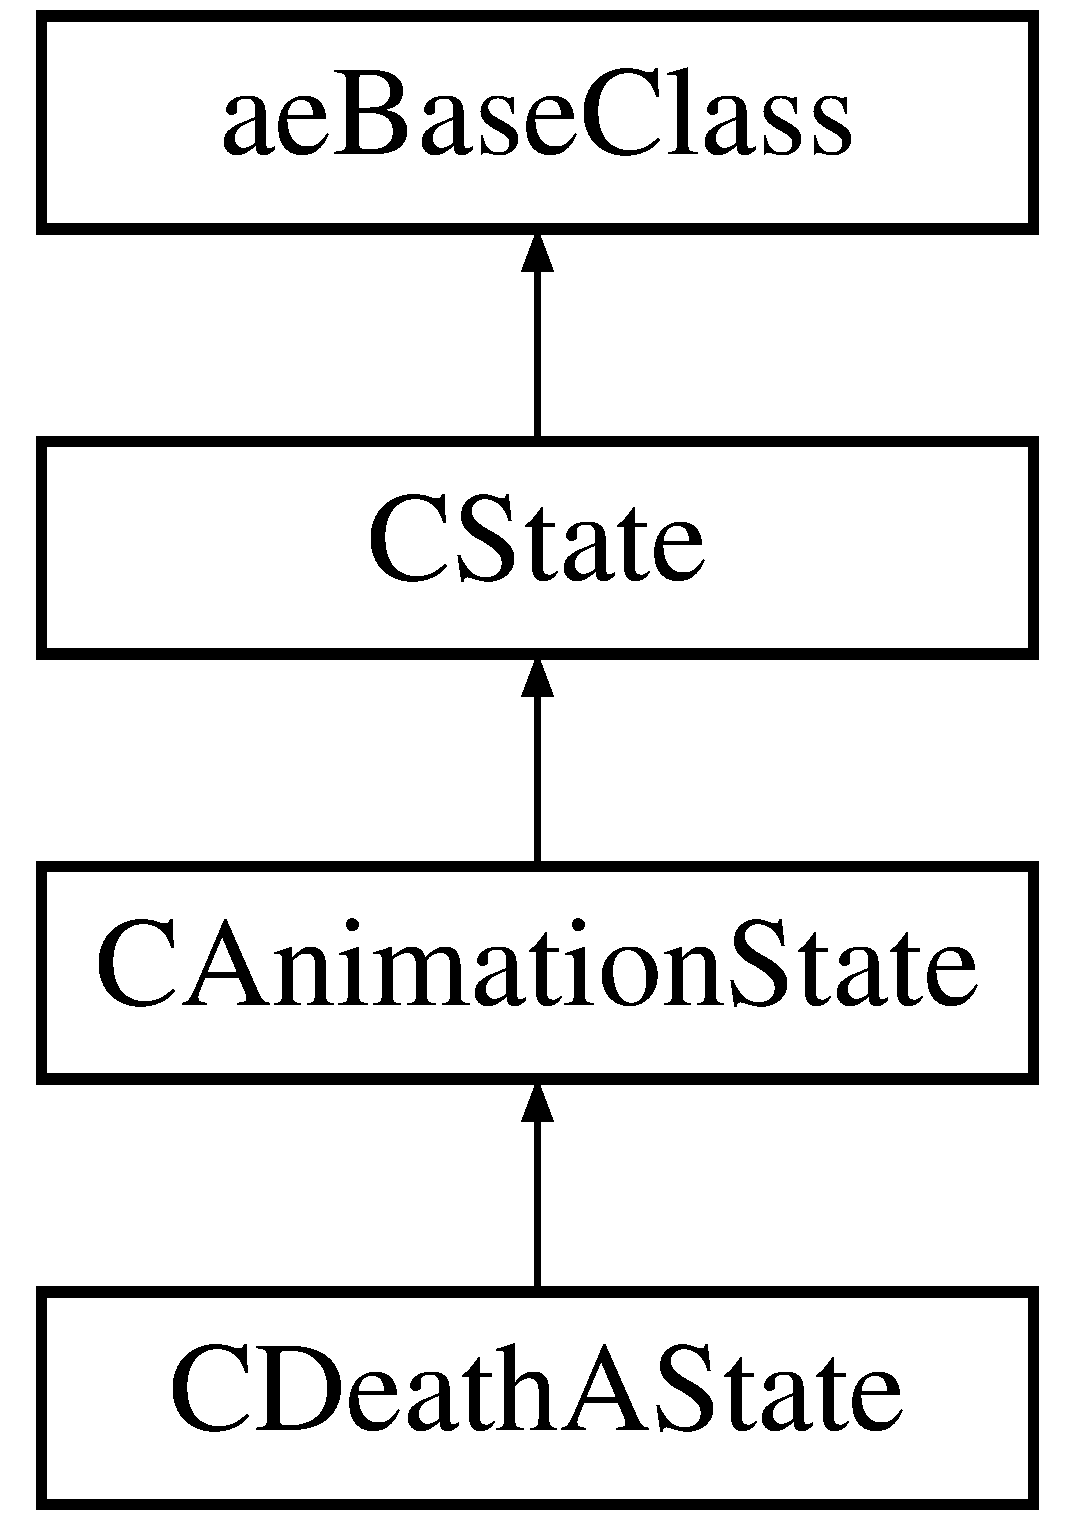
\includegraphics[height=4.000000cm]{class_c_death_a_state}
\end{center}
\end{figure}
\subsection*{Public Member Functions}
\begin{DoxyCompactItemize}
\item 
virtual void \hyperlink{class_c_death_a_state_a408f2b12e1cdb9f74704a23900480883}{Init} (\hyperlink{classae_state_machine_script}{ae\+State\+Machine\+Script} $\ast$p\+Script)
\begin{DoxyCompactList}\small\item\em Initializes the with the given state machine script. \end{DoxyCompactList}\item 
virtual void \hyperlink{class_c_death_a_state_a4a72bc7cb8bb7542f76a58749cbdd5de}{Destroy} ()\hypertarget{class_c_death_a_state_a4a72bc7cb8bb7542f76a58749cbdd5de}{}\label{class_c_death_a_state_a4a72bc7cb8bb7542f76a58749cbdd5de}

\begin{DoxyCompactList}\small\item\em Destroys this object. \end{DoxyCompactList}\item 
virtual int \hyperlink{class_c_death_a_state_ab2365bfffb1f627393e90e138e33bdaf}{On\+Update} (float f\+Delta, \hyperlink{classae_base_class}{ae\+Base\+Class} $\ast$p\+Object)
\begin{DoxyCompactList}\small\item\em Executes the update action. \end{DoxyCompactList}\item 
virtual void \hyperlink{class_c_death_a_state_a44b95f6bc0cfdc2204c11c851ab53c8e}{On\+Enter} ()\hypertarget{class_c_death_a_state_a44b95f6bc0cfdc2204c11c851ab53c8e}{}\label{class_c_death_a_state_a44b95f6bc0cfdc2204c11c851ab53c8e}

\begin{DoxyCompactList}\small\item\em Executes the enter action. \end{DoxyCompactList}\item 
virtual void \hyperlink{class_c_death_a_state_a4688c28a4243df74c67d85bd9b2bc061}{On\+Exit} ()\hypertarget{class_c_death_a_state_a4688c28a4243df74c67d85bd9b2bc061}{}\label{class_c_death_a_state_a4688c28a4243df74c67d85bd9b2bc061}

\begin{DoxyCompactList}\small\item\em Executes the exit action. \end{DoxyCompactList}\end{DoxyCompactItemize}
\subsection*{Additional Inherited Members}


\subsection{Member Function Documentation}
\index{C\+Death\+A\+State@{C\+Death\+A\+State}!Init@{Init}}
\index{Init@{Init}!C\+Death\+A\+State@{C\+Death\+A\+State}}
\subsubsection[{\texorpdfstring{Init(ae\+State\+Machine\+Script $\ast$p\+Script)}{Init(aeStateMachineScript *pScript)}}]{\setlength{\rightskip}{0pt plus 5cm}void C\+Death\+A\+State\+::\+Init (
\begin{DoxyParamCaption}
\item[{{\bf ae\+State\+Machine\+Script} $\ast$}]{p\+Script}
\end{DoxyParamCaption}
)\hspace{0.3cm}{\ttfamily [virtual]}}\hypertarget{class_c_death_a_state_a408f2b12e1cdb9f74704a23900480883}{}\label{class_c_death_a_state_a408f2b12e1cdb9f74704a23900480883}


Initializes the with the given state machine script. 


\begin{DoxyParams}[1]{Parameters}
\mbox{\tt in,out}  & {\em p\+Script} & If non-\/null, the script. \\
\hline
\end{DoxyParams}


Implements \hyperlink{class_c_state_a220fab97e545680a7237dbb0d04ba037}{C\+State}.

\index{C\+Death\+A\+State@{C\+Death\+A\+State}!On\+Update@{On\+Update}}
\index{On\+Update@{On\+Update}!C\+Death\+A\+State@{C\+Death\+A\+State}}
\subsubsection[{\texorpdfstring{On\+Update(float f\+Delta, ae\+Base\+Class $\ast$p\+Object)}{OnUpdate(float fDelta, aeBaseClass *pObject)}}]{\setlength{\rightskip}{0pt plus 5cm}int C\+Death\+A\+State\+::\+On\+Update (
\begin{DoxyParamCaption}
\item[{float}]{f\+Delta, }
\item[{{\bf ae\+Base\+Class} $\ast$}]{p\+Object}
\end{DoxyParamCaption}
)\hspace{0.3cm}{\ttfamily [virtual]}}\hypertarget{class_c_death_a_state_ab2365bfffb1f627393e90e138e33bdaf}{}\label{class_c_death_a_state_ab2365bfffb1f627393e90e138e33bdaf}


Executes the update action. 


\begin{DoxyParams}[1]{Parameters}
 & {\em f\+Delta} & The delta. \\
\hline
\mbox{\tt in,out}  & {\em p\+Object} & If non-\/null, the object.\\
\hline
\end{DoxyParams}
\begin{DoxyReturn}{Returns}
An int. 
\end{DoxyReturn}


Implements \hyperlink{class_c_state_a9d687e06b17b821703332fa3d4ea8bcf}{C\+State}.



The documentation for this class was generated from the following files\+:\begin{DoxyCompactItemize}
\item 
C\+:/\+Users/\+Alvaro Estrada/\+Documents/\+Visual Studio 2015/\+Projects/\+R\+T\+S\+\_\+\+A\+E/\+R\+T\+S\+\_\+\+A\+E/\+Game/Death\+A\+State.\+h\item 
C\+:/\+Users/\+Alvaro Estrada/\+Documents/\+Visual Studio 2015/\+Projects/\+R\+T\+S\+\_\+\+A\+E/\+R\+T\+S\+\_\+\+A\+E/\+Game/Death\+A\+State.\+cpp\end{DoxyCompactItemize}

\hypertarget{class_c_idle}{}\section{C\+Idle Class Reference}
\label{class_c_idle}\index{C\+Idle@{C\+Idle}}
Inheritance diagram for C\+Idle\+:\begin{figure}[H]
\begin{center}
\leavevmode
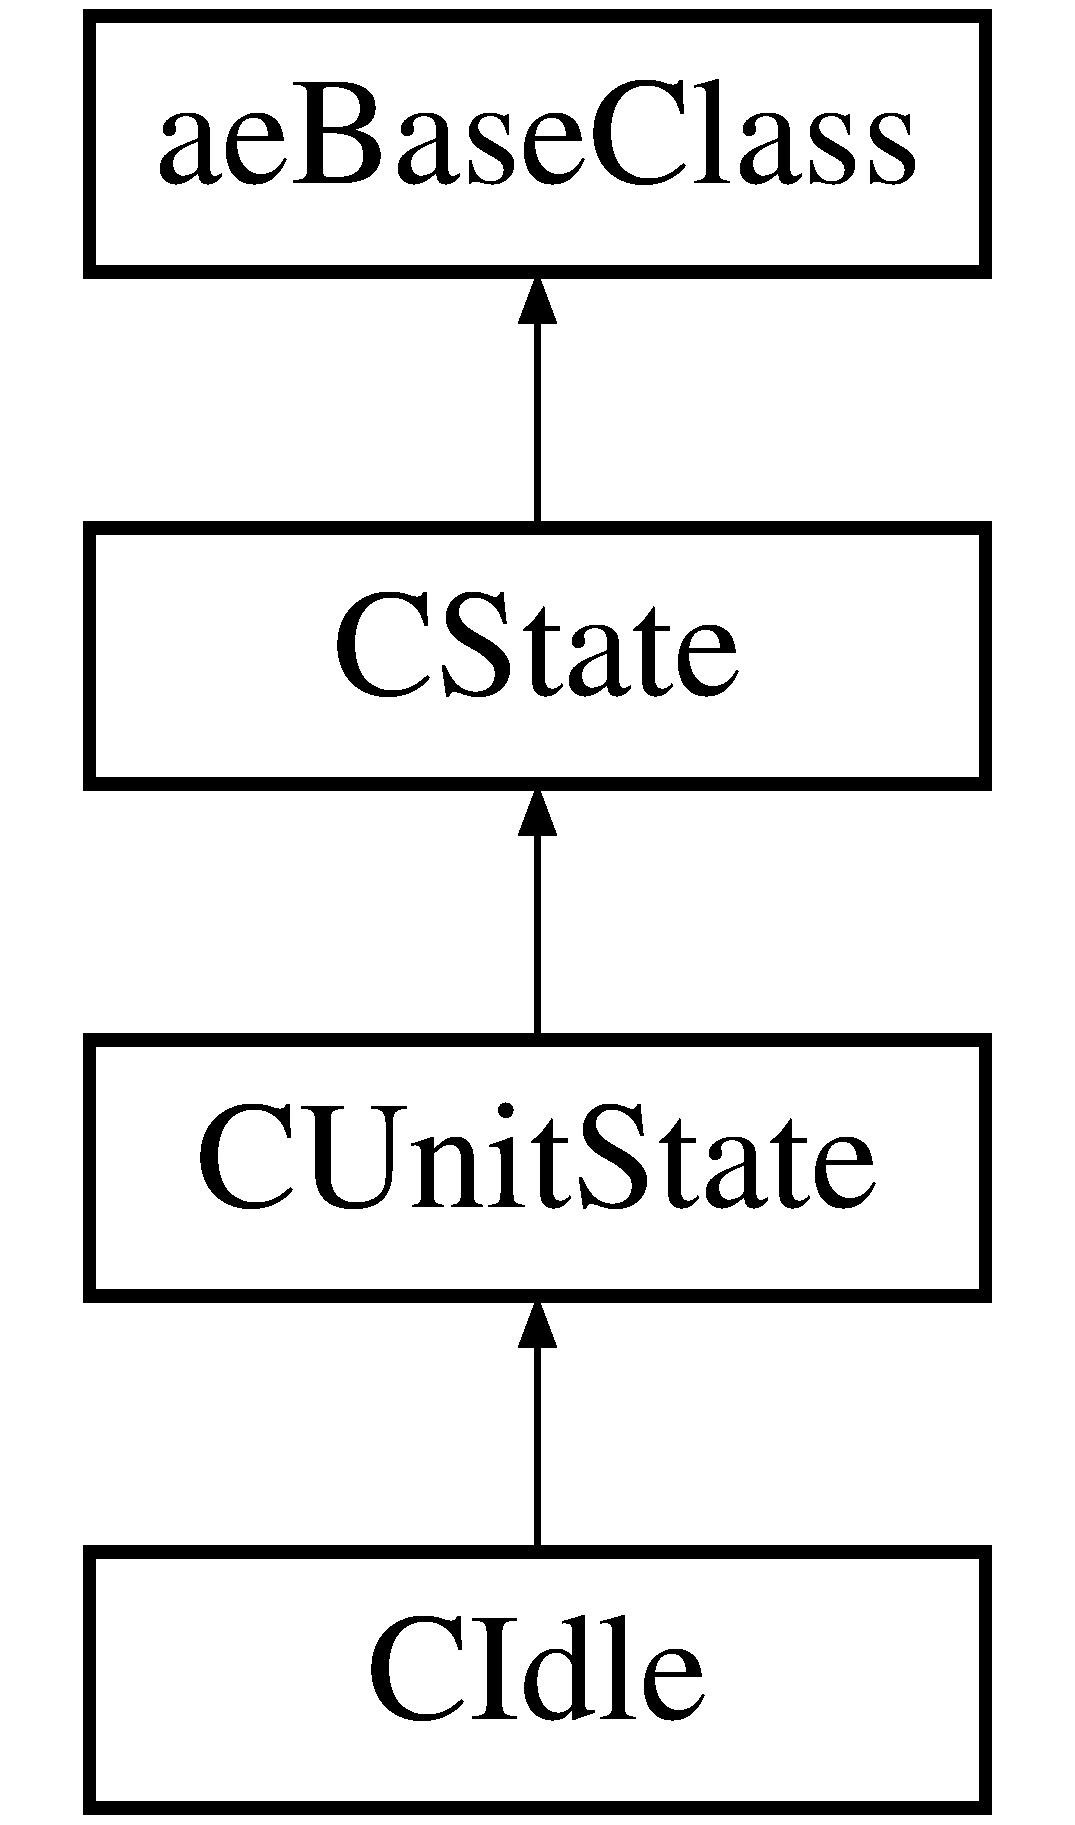
\includegraphics[height=4.000000cm]{class_c_idle}
\end{center}
\end{figure}
\subsection*{Public Member Functions}
\begin{DoxyCompactItemize}
\item 
virtual void \hyperlink{class_c_idle_a5f5632a117a51e37511142dffcea561e}{Init} (\hyperlink{classae_state_machine_script}{ae\+State\+Machine\+Script} $\ast$p\+Script)
\begin{DoxyCompactList}\small\item\em Initializes the with the given state machine script. \end{DoxyCompactList}\item 
virtual void \hyperlink{class_c_idle_aeb559d7cdbd4ff820a612da72ed808d6}{Destroy} ()\hypertarget{class_c_idle_aeb559d7cdbd4ff820a612da72ed808d6}{}\label{class_c_idle_aeb559d7cdbd4ff820a612da72ed808d6}

\begin{DoxyCompactList}\small\item\em Destroys this object. \end{DoxyCompactList}\item 
virtual int \hyperlink{class_c_idle_a32a095912ae94e7a9bcdfc8d3d3191db}{On\+Update} (float f\+Delta, \hyperlink{classae_base_class}{ae\+Base\+Class} $\ast$p\+Object)
\begin{DoxyCompactList}\small\item\em Executes the update action. \end{DoxyCompactList}\item 
virtual void \hyperlink{class_c_idle_aa143be4536dfe39f1c4efd0b88fedf2e}{On\+Enter} ()\hypertarget{class_c_idle_aa143be4536dfe39f1c4efd0b88fedf2e}{}\label{class_c_idle_aa143be4536dfe39f1c4efd0b88fedf2e}

\begin{DoxyCompactList}\small\item\em Executes the enter action. \end{DoxyCompactList}\item 
virtual void \hyperlink{class_c_idle_ac74d942d948f5a9c917b30c62a6c1d1d}{On\+Exit} ()\hypertarget{class_c_idle_ac74d942d948f5a9c917b30c62a6c1d1d}{}\label{class_c_idle_ac74d942d948f5a9c917b30c62a6c1d1d}

\begin{DoxyCompactList}\small\item\em Executes the exit action. \end{DoxyCompactList}\end{DoxyCompactItemize}
\subsection*{Additional Inherited Members}


\subsection{Member Function Documentation}
\index{C\+Idle@{C\+Idle}!Init@{Init}}
\index{Init@{Init}!C\+Idle@{C\+Idle}}
\subsubsection[{\texorpdfstring{Init(ae\+State\+Machine\+Script $\ast$p\+Script)}{Init(aeStateMachineScript *pScript)}}]{\setlength{\rightskip}{0pt plus 5cm}void C\+Idle\+::\+Init (
\begin{DoxyParamCaption}
\item[{{\bf ae\+State\+Machine\+Script} $\ast$}]{p\+Script}
\end{DoxyParamCaption}
)\hspace{0.3cm}{\ttfamily [virtual]}}\hypertarget{class_c_idle_a5f5632a117a51e37511142dffcea561e}{}\label{class_c_idle_a5f5632a117a51e37511142dffcea561e}


Initializes the with the given state machine script. 


\begin{DoxyParams}[1]{Parameters}
\mbox{\tt in,out}  & {\em p\+Script} & If non-\/null, the script. \\
\hline
\end{DoxyParams}


Implements \hyperlink{class_c_state_a220fab97e545680a7237dbb0d04ba037}{C\+State}.

\index{C\+Idle@{C\+Idle}!On\+Update@{On\+Update}}
\index{On\+Update@{On\+Update}!C\+Idle@{C\+Idle}}
\subsubsection[{\texorpdfstring{On\+Update(float f\+Delta, ae\+Base\+Class $\ast$p\+Object)}{OnUpdate(float fDelta, aeBaseClass *pObject)}}]{\setlength{\rightskip}{0pt plus 5cm}int C\+Idle\+::\+On\+Update (
\begin{DoxyParamCaption}
\item[{float}]{f\+Delta, }
\item[{{\bf ae\+Base\+Class} $\ast$}]{p\+Object}
\end{DoxyParamCaption}
)\hspace{0.3cm}{\ttfamily [virtual]}}\hypertarget{class_c_idle_a32a095912ae94e7a9bcdfc8d3d3191db}{}\label{class_c_idle_a32a095912ae94e7a9bcdfc8d3d3191db}


Executes the update action. 


\begin{DoxyParams}[1]{Parameters}
 & {\em f\+Delta} & The delta. \\
\hline
\mbox{\tt in,out}  & {\em p\+Object} & If non-\/null, the object.\\
\hline
\end{DoxyParams}
\begin{DoxyReturn}{Returns}
An int. 
\end{DoxyReturn}


Implements \hyperlink{class_c_state_a9d687e06b17b821703332fa3d4ea8bcf}{C\+State}.



The documentation for this class was generated from the following files\+:\begin{DoxyCompactItemize}
\item 
C\+:/\+Users/\+Alvaro Estrada/\+Documents/\+Visual Studio 2015/\+Projects/\+R\+T\+S\+\_\+\+A\+E/\+R\+T\+S\+\_\+\+A\+E/\+Game/Idle.\+h\item 
C\+:/\+Users/\+Alvaro Estrada/\+Documents/\+Visual Studio 2015/\+Projects/\+R\+T\+S\+\_\+\+A\+E/\+R\+T\+S\+\_\+\+A\+E/\+Game/Idle.\+cpp\end{DoxyCompactItemize}

\hypertarget{class_c_idle_a_state}{}\section{C\+Idle\+A\+State Class Reference}
\label{class_c_idle_a_state}\index{C\+Idle\+A\+State@{C\+Idle\+A\+State}}
Inheritance diagram for C\+Idle\+A\+State\+:\begin{figure}[H]
\begin{center}
\leavevmode
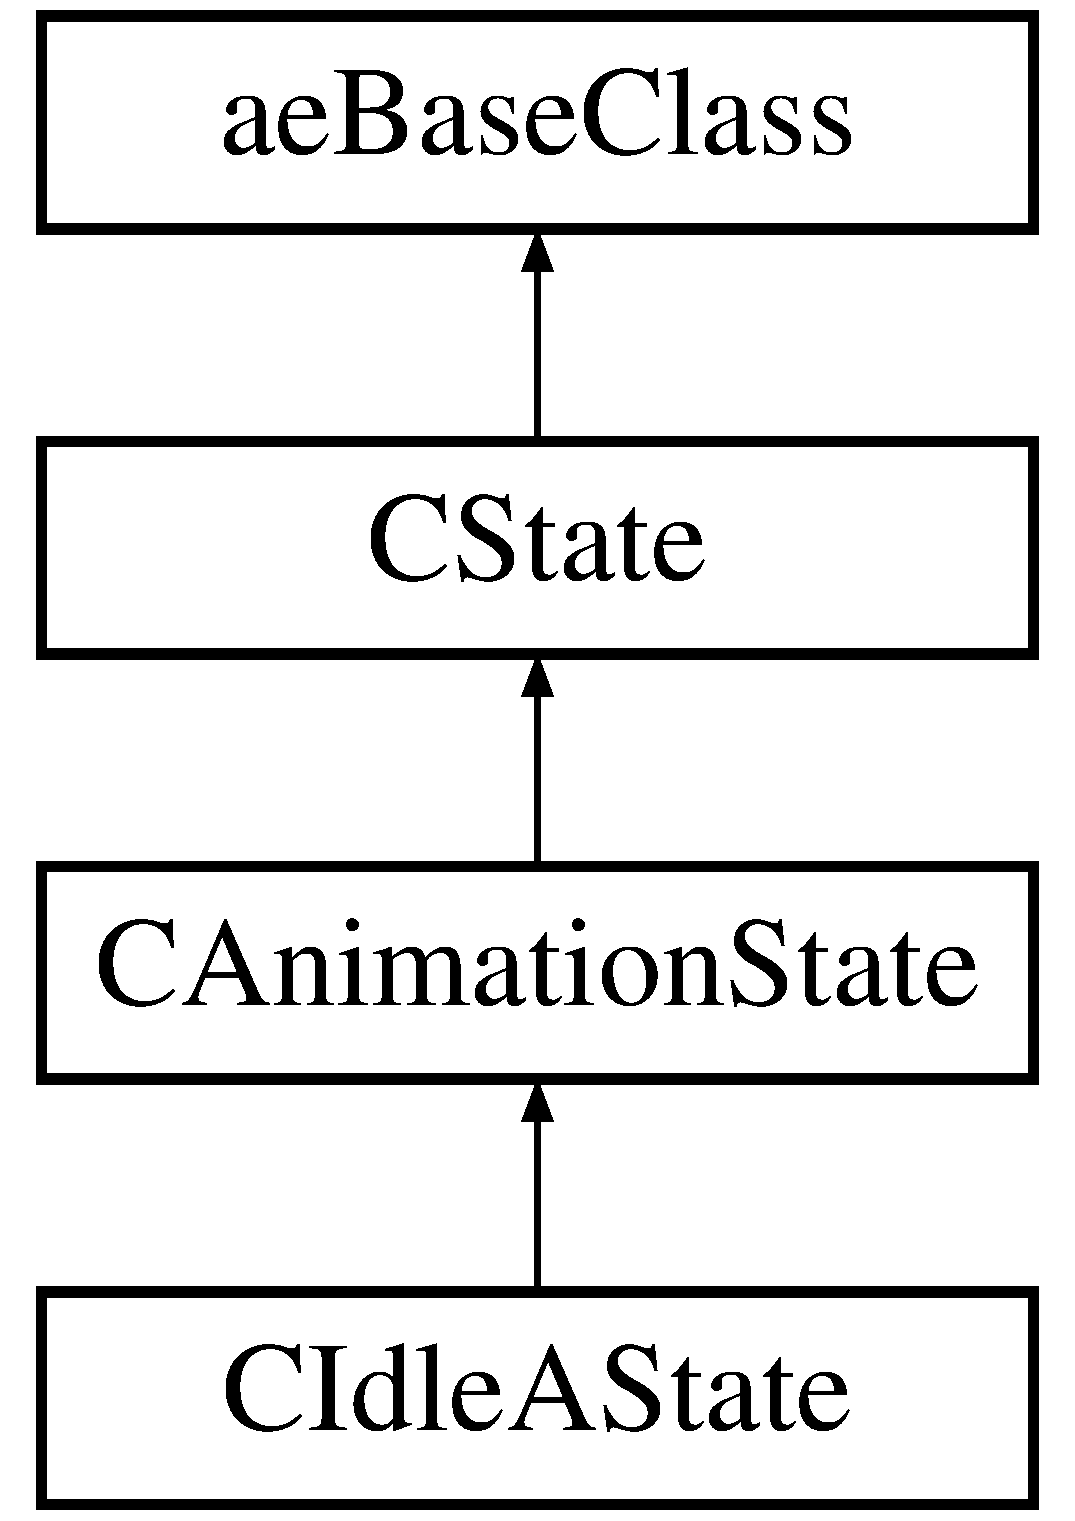
\includegraphics[height=4.000000cm]{class_c_idle_a_state}
\end{center}
\end{figure}
\subsection*{Public Member Functions}
\begin{DoxyCompactItemize}
\item 
virtual void \hyperlink{class_c_idle_a_state_a241993e2f04379b3027657011eed870b}{Init} (\hyperlink{classae_state_machine_script}{ae\+State\+Machine\+Script} $\ast$p\+Script)
\begin{DoxyCompactList}\small\item\em Initializes the with the given state machine script. \end{DoxyCompactList}\item 
virtual void \hyperlink{class_c_idle_a_state_a2da54a475a63aeed335bdc67967587ad}{Destroy} ()\hypertarget{class_c_idle_a_state_a2da54a475a63aeed335bdc67967587ad}{}\label{class_c_idle_a_state_a2da54a475a63aeed335bdc67967587ad}

\begin{DoxyCompactList}\small\item\em Destroys this object. \end{DoxyCompactList}\item 
virtual int \hyperlink{class_c_idle_a_state_aa68dafffda29e2bce8b37a79a515e353}{On\+Update} (float f\+Delta, \hyperlink{classae_base_class}{ae\+Base\+Class} $\ast$p\+Object)
\begin{DoxyCompactList}\small\item\em Executes the update action. \end{DoxyCompactList}\item 
virtual void \hyperlink{class_c_idle_a_state_abea7da5d0146d6527bd08553b97e4ab4}{On\+Enter} ()\hypertarget{class_c_idle_a_state_abea7da5d0146d6527bd08553b97e4ab4}{}\label{class_c_idle_a_state_abea7da5d0146d6527bd08553b97e4ab4}

\begin{DoxyCompactList}\small\item\em Executes the enter action. \end{DoxyCompactList}\item 
virtual void \hyperlink{class_c_idle_a_state_a6574794990f717dbac0b7806144581d9}{On\+Exit} ()\hypertarget{class_c_idle_a_state_a6574794990f717dbac0b7806144581d9}{}\label{class_c_idle_a_state_a6574794990f717dbac0b7806144581d9}

\begin{DoxyCompactList}\small\item\em Executes the exit action. \end{DoxyCompactList}\end{DoxyCompactItemize}
\subsection*{Additional Inherited Members}


\subsection{Member Function Documentation}
\index{C\+Idle\+A\+State@{C\+Idle\+A\+State}!Init@{Init}}
\index{Init@{Init}!C\+Idle\+A\+State@{C\+Idle\+A\+State}}
\subsubsection[{\texorpdfstring{Init(ae\+State\+Machine\+Script $\ast$p\+Script)}{Init(aeStateMachineScript *pScript)}}]{\setlength{\rightskip}{0pt plus 5cm}void C\+Idle\+A\+State\+::\+Init (
\begin{DoxyParamCaption}
\item[{{\bf ae\+State\+Machine\+Script} $\ast$}]{p\+Script}
\end{DoxyParamCaption}
)\hspace{0.3cm}{\ttfamily [virtual]}}\hypertarget{class_c_idle_a_state_a241993e2f04379b3027657011eed870b}{}\label{class_c_idle_a_state_a241993e2f04379b3027657011eed870b}


Initializes the with the given state machine script. 


\begin{DoxyParams}[1]{Parameters}
\mbox{\tt in,out}  & {\em p\+Script} & If non-\/null, the script. \\
\hline
\end{DoxyParams}


Implements \hyperlink{class_c_state_a220fab97e545680a7237dbb0d04ba037}{C\+State}.

\index{C\+Idle\+A\+State@{C\+Idle\+A\+State}!On\+Update@{On\+Update}}
\index{On\+Update@{On\+Update}!C\+Idle\+A\+State@{C\+Idle\+A\+State}}
\subsubsection[{\texorpdfstring{On\+Update(float f\+Delta, ae\+Base\+Class $\ast$p\+Object)}{OnUpdate(float fDelta, aeBaseClass *pObject)}}]{\setlength{\rightskip}{0pt plus 5cm}int C\+Idle\+A\+State\+::\+On\+Update (
\begin{DoxyParamCaption}
\item[{float}]{f\+Delta, }
\item[{{\bf ae\+Base\+Class} $\ast$}]{p\+Object}
\end{DoxyParamCaption}
)\hspace{0.3cm}{\ttfamily [virtual]}}\hypertarget{class_c_idle_a_state_aa68dafffda29e2bce8b37a79a515e353}{}\label{class_c_idle_a_state_aa68dafffda29e2bce8b37a79a515e353}


Executes the update action. 


\begin{DoxyParams}[1]{Parameters}
 & {\em f\+Delta} & The delta. \\
\hline
\mbox{\tt in,out}  & {\em p\+Object} & If non-\/null, the object.\\
\hline
\end{DoxyParams}
\begin{DoxyReturn}{Returns}
An int. 
\end{DoxyReturn}


Implements \hyperlink{class_c_state_a9d687e06b17b821703332fa3d4ea8bcf}{C\+State}.



The documentation for this class was generated from the following files\+:\begin{DoxyCompactItemize}
\item 
C\+:/\+Users/\+Alvaro Estrada/\+Documents/\+Visual Studio 2015/\+Projects/\+R\+T\+S\+\_\+\+A\+E/\+R\+T\+S\+\_\+\+A\+E/\+Game/Idle\+A\+State.\+h\item 
C\+:/\+Users/\+Alvaro Estrada/\+Documents/\+Visual Studio 2015/\+Projects/\+R\+T\+S\+\_\+\+A\+E/\+R\+T\+S\+\_\+\+A\+E/\+Game/Idle\+A\+State.\+cpp\end{DoxyCompactItemize}

\hypertarget{class_c_move___to}{}\section{C\+Move\+\_\+\+To Class Reference}
\label{class_c_move___to}\index{C\+Move\+\_\+\+To@{C\+Move\+\_\+\+To}}
Inheritance diagram for C\+Move\+\_\+\+To\+:\begin{figure}[H]
\begin{center}
\leavevmode
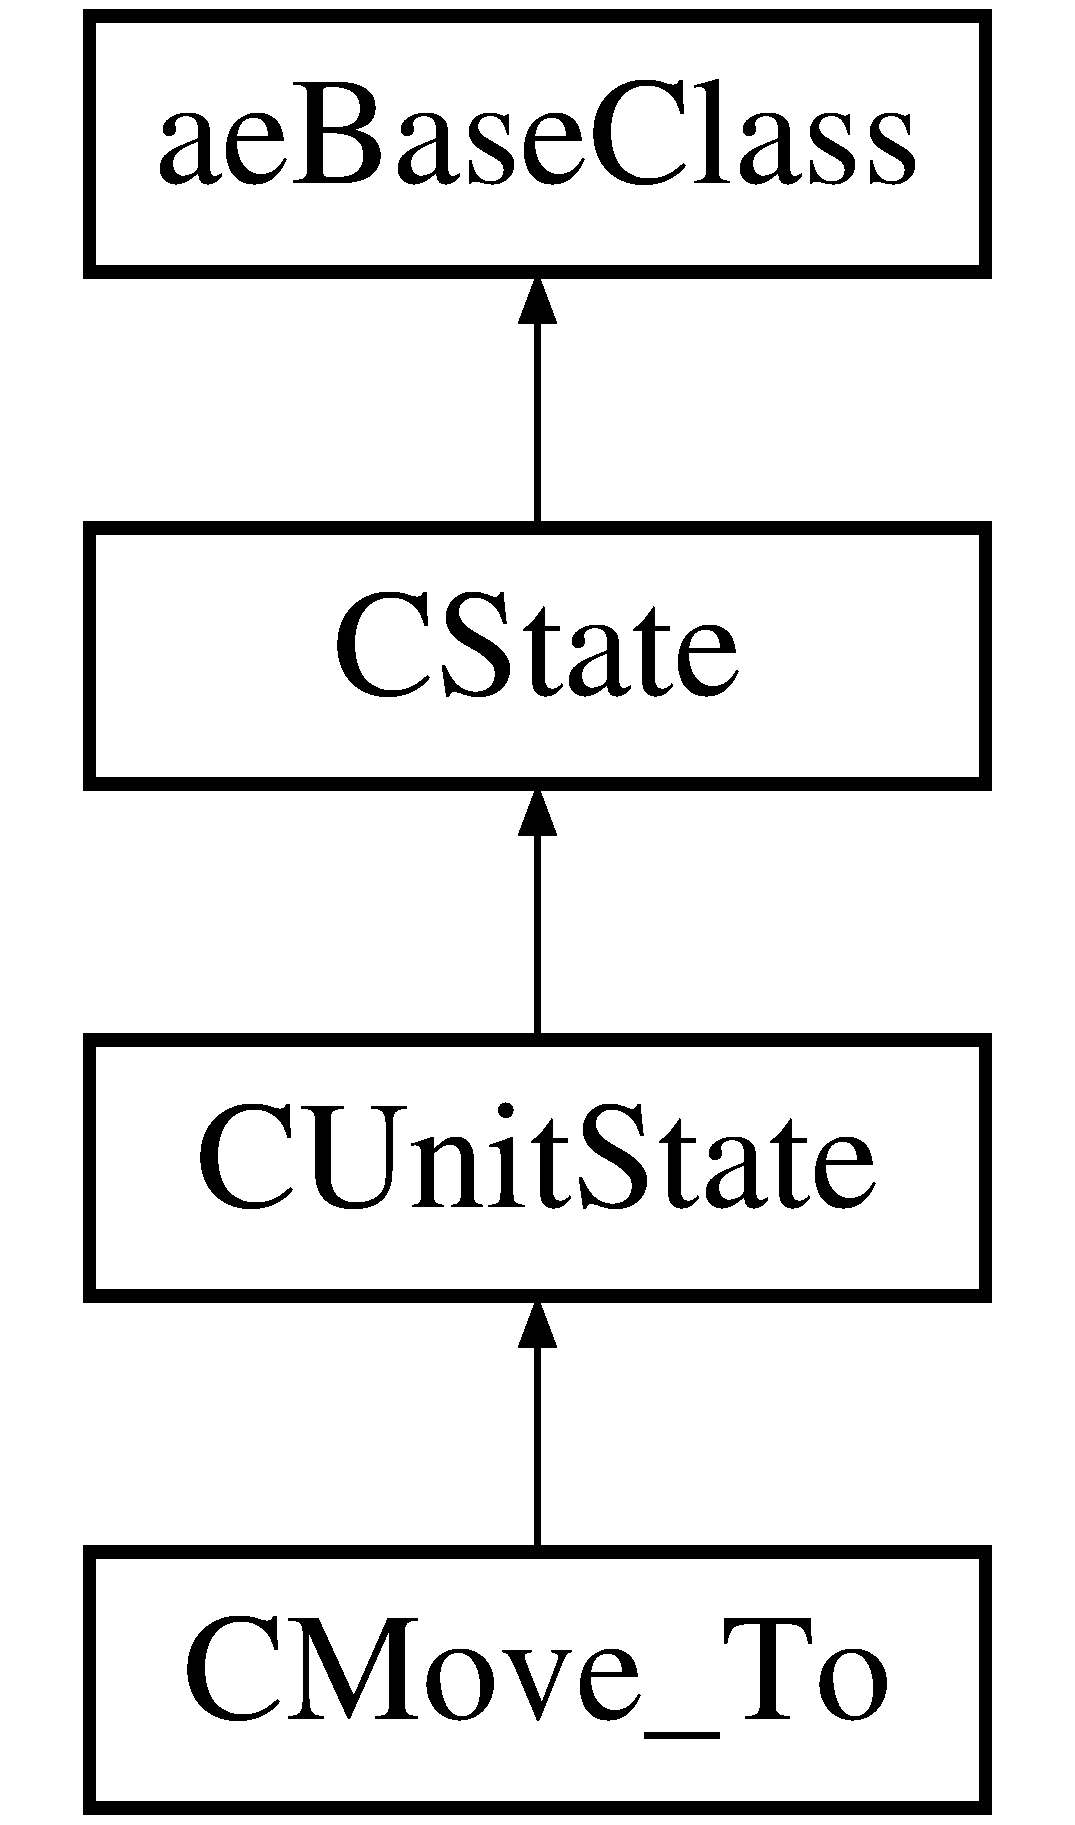
\includegraphics[height=4.000000cm]{class_c_move___to}
\end{center}
\end{figure}
\subsection*{Public Member Functions}
\begin{DoxyCompactItemize}
\item 
virtual void \hyperlink{class_c_move___to_a1fdf0a3aaa63c1f1eebb51664d00a01f}{Init} (\hyperlink{classae_state_machine_script}{ae\+State\+Machine\+Script} $\ast$p\+Script)
\begin{DoxyCompactList}\small\item\em Initializes the with the given state machine script. \end{DoxyCompactList}\item 
virtual void \hyperlink{class_c_move___to_ad9f7f295a7a54c51a729d7828923eecc}{Destroy} ()\hypertarget{class_c_move___to_ad9f7f295a7a54c51a729d7828923eecc}{}\label{class_c_move___to_ad9f7f295a7a54c51a729d7828923eecc}

\begin{DoxyCompactList}\small\item\em Destroys this object. \end{DoxyCompactList}\item 
virtual int \hyperlink{class_c_move___to_aff66ed974bd3a4924b5bb35966d81300}{On\+Update} (float f\+Delta, \hyperlink{classae_base_class}{ae\+Base\+Class} $\ast$p\+Object)
\begin{DoxyCompactList}\small\item\em Executes the update action. \end{DoxyCompactList}\item 
virtual void \hyperlink{class_c_move___to_ac4f4e04e228f89904ef03e23165dc400}{On\+Enter} ()\hypertarget{class_c_move___to_ac4f4e04e228f89904ef03e23165dc400}{}\label{class_c_move___to_ac4f4e04e228f89904ef03e23165dc400}

\begin{DoxyCompactList}\small\item\em Executes the enter action. \end{DoxyCompactList}\item 
virtual void \hyperlink{class_c_move___to_ab42bcce382861d80ecfff9d8e041dc28}{On\+Exit} ()\hypertarget{class_c_move___to_ab42bcce382861d80ecfff9d8e041dc28}{}\label{class_c_move___to_ab42bcce382861d80ecfff9d8e041dc28}

\begin{DoxyCompactList}\small\item\em Executes the exit action. \end{DoxyCompactList}\end{DoxyCompactItemize}
\subsection*{Additional Inherited Members}


\subsection{Member Function Documentation}
\index{C\+Move\+\_\+\+To@{C\+Move\+\_\+\+To}!Init@{Init}}
\index{Init@{Init}!C\+Move\+\_\+\+To@{C\+Move\+\_\+\+To}}
\subsubsection[{\texorpdfstring{Init(ae\+State\+Machine\+Script $\ast$p\+Script)}{Init(aeStateMachineScript *pScript)}}]{\setlength{\rightskip}{0pt plus 5cm}void C\+Move\+\_\+\+To\+::\+Init (
\begin{DoxyParamCaption}
\item[{{\bf ae\+State\+Machine\+Script} $\ast$}]{p\+Script}
\end{DoxyParamCaption}
)\hspace{0.3cm}{\ttfamily [virtual]}}\hypertarget{class_c_move___to_a1fdf0a3aaa63c1f1eebb51664d00a01f}{}\label{class_c_move___to_a1fdf0a3aaa63c1f1eebb51664d00a01f}


Initializes the with the given state machine script. 


\begin{DoxyParams}[1]{Parameters}
\mbox{\tt in,out}  & {\em p\+Script} & If non-\/null, the script. \\
\hline
\end{DoxyParams}


Implements \hyperlink{class_c_state_a220fab97e545680a7237dbb0d04ba037}{C\+State}.

\index{C\+Move\+\_\+\+To@{C\+Move\+\_\+\+To}!On\+Update@{On\+Update}}
\index{On\+Update@{On\+Update}!C\+Move\+\_\+\+To@{C\+Move\+\_\+\+To}}
\subsubsection[{\texorpdfstring{On\+Update(float f\+Delta, ae\+Base\+Class $\ast$p\+Object)}{OnUpdate(float fDelta, aeBaseClass *pObject)}}]{\setlength{\rightskip}{0pt plus 5cm}int C\+Move\+\_\+\+To\+::\+On\+Update (
\begin{DoxyParamCaption}
\item[{float}]{f\+Delta, }
\item[{{\bf ae\+Base\+Class} $\ast$}]{p\+Object}
\end{DoxyParamCaption}
)\hspace{0.3cm}{\ttfamily [virtual]}}\hypertarget{class_c_move___to_aff66ed974bd3a4924b5bb35966d81300}{}\label{class_c_move___to_aff66ed974bd3a4924b5bb35966d81300}


Executes the update action. 


\begin{DoxyParams}[1]{Parameters}
 & {\em f\+Delta} & The delta. \\
\hline
\mbox{\tt in,out}  & {\em p\+Object} & If non-\/null, the object.\\
\hline
\end{DoxyParams}
\begin{DoxyReturn}{Returns}
An int. 
\end{DoxyReturn}


Implements \hyperlink{class_c_state_a9d687e06b17b821703332fa3d4ea8bcf}{C\+State}.



The documentation for this class was generated from the following files\+:\begin{DoxyCompactItemize}
\item 
C\+:/\+Users/\+Alvaro Estrada/\+Documents/\+Visual Studio 2015/\+Projects/\+R\+T\+S\+\_\+\+A\+E/\+R\+T\+S\+\_\+\+A\+E/\+Game/Move\+\_\+\+To.\+h\item 
C\+:/\+Users/\+Alvaro Estrada/\+Documents/\+Visual Studio 2015/\+Projects/\+R\+T\+S\+\_\+\+A\+E/\+R\+T\+S\+\_\+\+A\+E/\+Game/Move\+\_\+\+To.\+cpp\end{DoxyCompactItemize}

\hypertarget{class_c_move_to_a_state}{}\section{C\+Move\+To\+A\+State Class Reference}
\label{class_c_move_to_a_state}\index{C\+Move\+To\+A\+State@{C\+Move\+To\+A\+State}}
Inheritance diagram for C\+Move\+To\+A\+State\+:\begin{figure}[H]
\begin{center}
\leavevmode
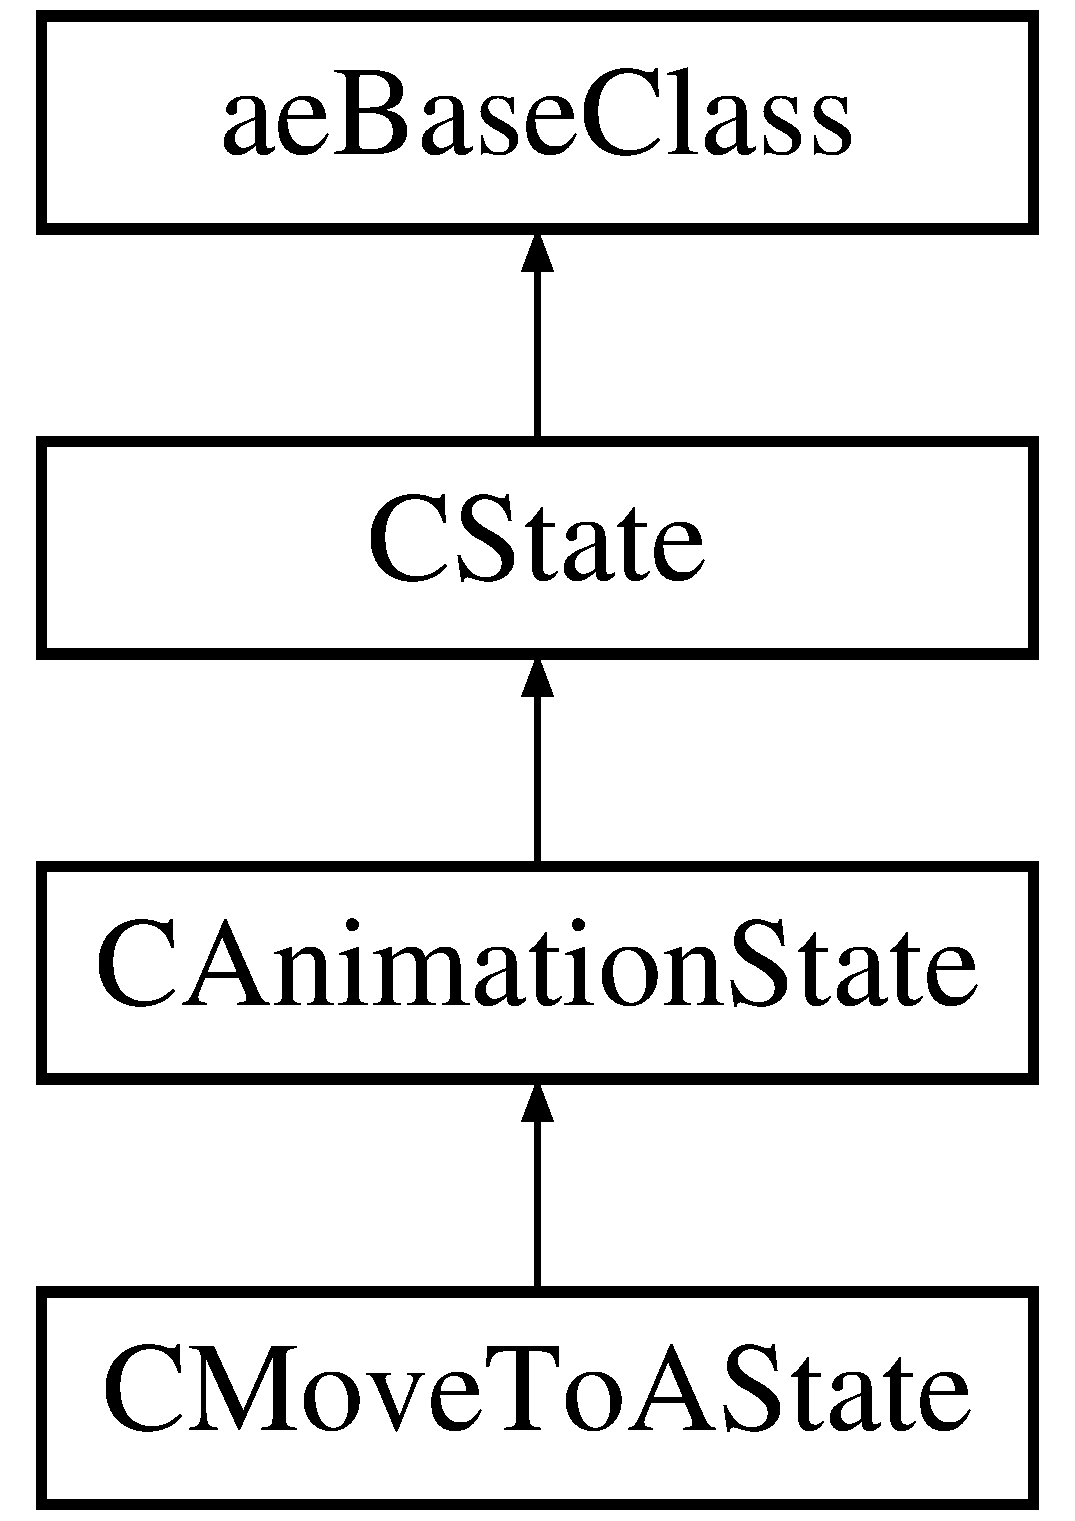
\includegraphics[height=4.000000cm]{class_c_move_to_a_state}
\end{center}
\end{figure}
\subsection*{Public Member Functions}
\begin{DoxyCompactItemize}
\item 
virtual void \hyperlink{class_c_move_to_a_state_ac0d824abba75c038600b4a6dc6a9d1c6}{Init} (\hyperlink{classae_state_machine_script}{ae\+State\+Machine\+Script} $\ast$p\+Script)
\begin{DoxyCompactList}\small\item\em Initializes the with the given state machine script. \end{DoxyCompactList}\item 
virtual void \hyperlink{class_c_move_to_a_state_adaf63cd9456e37d3db563c626e77fca7}{Destroy} ()\hypertarget{class_c_move_to_a_state_adaf63cd9456e37d3db563c626e77fca7}{}\label{class_c_move_to_a_state_adaf63cd9456e37d3db563c626e77fca7}

\begin{DoxyCompactList}\small\item\em Destroys this object. \end{DoxyCompactList}\item 
virtual int \hyperlink{class_c_move_to_a_state_a282f85cf10e81a233afbe9885a1a1d6e}{On\+Update} (float f\+Delta, \hyperlink{classae_base_class}{ae\+Base\+Class} $\ast$p\+Object)
\begin{DoxyCompactList}\small\item\em Executes the update action. \end{DoxyCompactList}\item 
virtual void \hyperlink{class_c_move_to_a_state_a4ca60d317b679ae6bbcc573358cc251d}{On\+Enter} ()\hypertarget{class_c_move_to_a_state_a4ca60d317b679ae6bbcc573358cc251d}{}\label{class_c_move_to_a_state_a4ca60d317b679ae6bbcc573358cc251d}

\begin{DoxyCompactList}\small\item\em Executes the enter action. \end{DoxyCompactList}\item 
virtual void \hyperlink{class_c_move_to_a_state_a878e781e8f2d9e6dc4030b1eac6bf6b4}{On\+Exit} ()\hypertarget{class_c_move_to_a_state_a878e781e8f2d9e6dc4030b1eac6bf6b4}{}\label{class_c_move_to_a_state_a878e781e8f2d9e6dc4030b1eac6bf6b4}

\begin{DoxyCompactList}\small\item\em Executes the exit action. \end{DoxyCompactList}\end{DoxyCompactItemize}
\subsection*{Additional Inherited Members}


\subsection{Member Function Documentation}
\index{C\+Move\+To\+A\+State@{C\+Move\+To\+A\+State}!Init@{Init}}
\index{Init@{Init}!C\+Move\+To\+A\+State@{C\+Move\+To\+A\+State}}
\subsubsection[{\texorpdfstring{Init(ae\+State\+Machine\+Script $\ast$p\+Script)}{Init(aeStateMachineScript *pScript)}}]{\setlength{\rightskip}{0pt plus 5cm}void C\+Move\+To\+A\+State\+::\+Init (
\begin{DoxyParamCaption}
\item[{{\bf ae\+State\+Machine\+Script} $\ast$}]{p\+Script}
\end{DoxyParamCaption}
)\hspace{0.3cm}{\ttfamily [virtual]}}\hypertarget{class_c_move_to_a_state_ac0d824abba75c038600b4a6dc6a9d1c6}{}\label{class_c_move_to_a_state_ac0d824abba75c038600b4a6dc6a9d1c6}


Initializes the with the given state machine script. 


\begin{DoxyParams}[1]{Parameters}
\mbox{\tt in,out}  & {\em p\+Script} & If non-\/null, the script. \\
\hline
\end{DoxyParams}


Implements \hyperlink{class_c_state_a220fab97e545680a7237dbb0d04ba037}{C\+State}.

\index{C\+Move\+To\+A\+State@{C\+Move\+To\+A\+State}!On\+Update@{On\+Update}}
\index{On\+Update@{On\+Update}!C\+Move\+To\+A\+State@{C\+Move\+To\+A\+State}}
\subsubsection[{\texorpdfstring{On\+Update(float f\+Delta, ae\+Base\+Class $\ast$p\+Object)}{OnUpdate(float fDelta, aeBaseClass *pObject)}}]{\setlength{\rightskip}{0pt plus 5cm}int C\+Move\+To\+A\+State\+::\+On\+Update (
\begin{DoxyParamCaption}
\item[{float}]{f\+Delta, }
\item[{{\bf ae\+Base\+Class} $\ast$}]{p\+Object}
\end{DoxyParamCaption}
)\hspace{0.3cm}{\ttfamily [virtual]}}\hypertarget{class_c_move_to_a_state_a282f85cf10e81a233afbe9885a1a1d6e}{}\label{class_c_move_to_a_state_a282f85cf10e81a233afbe9885a1a1d6e}


Executes the update action. 


\begin{DoxyParams}[1]{Parameters}
 & {\em f\+Delta} & The delta. \\
\hline
\mbox{\tt in,out}  & {\em p\+Object} & If non-\/null, the object.\\
\hline
\end{DoxyParams}
\begin{DoxyReturn}{Returns}
An int. 
\end{DoxyReturn}


Implements \hyperlink{class_c_state_a9d687e06b17b821703332fa3d4ea8bcf}{C\+State}.



The documentation for this class was generated from the following files\+:\begin{DoxyCompactItemize}
\item 
C\+:/\+Users/\+Alvaro Estrada/\+Documents/\+Visual Studio 2015/\+Projects/\+R\+T\+S\+\_\+\+A\+E/\+R\+T\+S\+\_\+\+A\+E/\+Game/Move\+To\+A\+State.\+h\item 
C\+:/\+Users/\+Alvaro Estrada/\+Documents/\+Visual Studio 2015/\+Projects/\+R\+T\+S\+\_\+\+A\+E/\+R\+T\+S\+\_\+\+A\+E/\+Game/Move\+To\+A\+State.\+cpp\end{DoxyCompactItemize}

\hypertarget{class_c_state}{}\section{C\+State Class Reference}
\label{class_c_state}\index{C\+State@{C\+State}}
Inheritance diagram for C\+State\+:\begin{figure}[H]
\begin{center}
\leavevmode
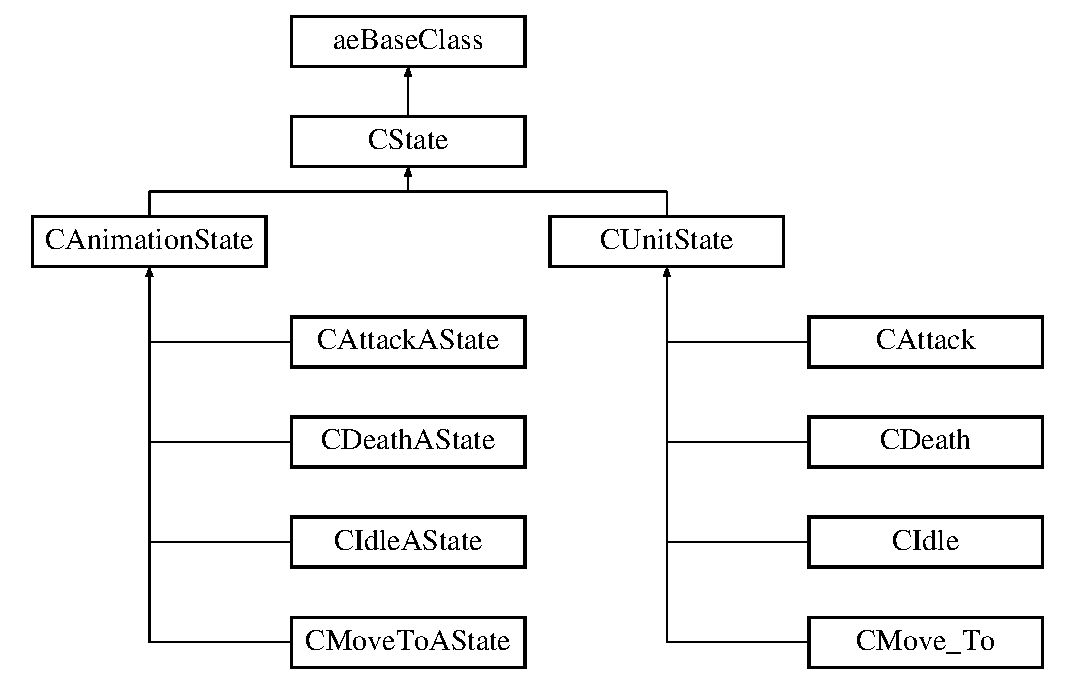
\includegraphics[height=7.000000cm]{class_c_state}
\end{center}
\end{figure}
\subsection*{Public Member Functions}
\begin{DoxyCompactItemize}
\item 
virtual void \hyperlink{class_c_state_a220fab97e545680a7237dbb0d04ba037}{Init} (\hyperlink{classae_state_machine_script}{ae\+State\+Machine\+Script} $\ast$p\+Script)=0
\begin{DoxyCompactList}\small\item\em Initializes the with the given state machine script. \end{DoxyCompactList}\item 
virtual void \hyperlink{class_c_state_ab51ebc6c91699f2b1a3b49e77fba9ebf}{Destroy} ()\hypertarget{class_c_state_ab51ebc6c91699f2b1a3b49e77fba9ebf}{}\label{class_c_state_ab51ebc6c91699f2b1a3b49e77fba9ebf}

\begin{DoxyCompactList}\small\item\em Destroys this object. \end{DoxyCompactList}\item 
virtual int \hyperlink{class_c_state_a9d687e06b17b821703332fa3d4ea8bcf}{On\+Update} (float f\+Delta, \hyperlink{classae_base_class}{ae\+Base\+Class} $\ast$p\+Object)=0
\begin{DoxyCompactList}\small\item\em Executes the update action. \end{DoxyCompactList}\item 
virtual void \hyperlink{class_c_state_aa243e28819ea28e4499a37ce88905f5a}{On\+Enter} ()=0\hypertarget{class_c_state_aa243e28819ea28e4499a37ce88905f5a}{}\label{class_c_state_aa243e28819ea28e4499a37ce88905f5a}

\begin{DoxyCompactList}\small\item\em Executes the enter action. \end{DoxyCompactList}\item 
virtual void \hyperlink{class_c_state_ad44fb6c87328ce8429f0a11fcb1546c9}{On\+Exit} ()=0\hypertarget{class_c_state_ad44fb6c87328ce8429f0a11fcb1546c9}{}\label{class_c_state_ad44fb6c87328ce8429f0a11fcb1546c9}

\begin{DoxyCompactList}\small\item\em Executes the exit action. \end{DoxyCompactList}\item 
bool \hyperlink{class_c_state_ab3ac73ec432c327da36cdaaabeb2ac76}{operator==} (int State\+ID)
\begin{DoxyCompactList}\small\item\em Equality operator. \end{DoxyCompactList}\end{DoxyCompactItemize}
\subsection*{Protected Attributes}
\begin{DoxyCompactItemize}
\item 
int {\bfseries m\+\_\+n\+State\+ID}\hypertarget{class_c_state_a7a5e683c31758ad8648f4e238b1d615b}{}\label{class_c_state_a7a5e683c31758ad8648f4e238b1d615b}

\end{DoxyCompactItemize}


\subsection{Member Function Documentation}
\index{C\+State@{C\+State}!Init@{Init}}
\index{Init@{Init}!C\+State@{C\+State}}
\subsubsection[{\texorpdfstring{Init(ae\+State\+Machine\+Script $\ast$p\+Script)=0}{Init(aeStateMachineScript *pScript)=0}}]{\setlength{\rightskip}{0pt plus 5cm}void C\+State\+::\+Init (
\begin{DoxyParamCaption}
\item[{{\bf ae\+State\+Machine\+Script} $\ast$}]{p\+Script}
\end{DoxyParamCaption}
)\hspace{0.3cm}{\ttfamily [pure virtual]}}\hypertarget{class_c_state_a220fab97e545680a7237dbb0d04ba037}{}\label{class_c_state_a220fab97e545680a7237dbb0d04ba037}


Initializes the with the given state machine script. 


\begin{DoxyParams}[1]{Parameters}
\mbox{\tt in,out}  & {\em p\+Script} & If non-\/null, the script. \\
\hline
\end{DoxyParams}


Implemented in \hyperlink{class_c_attack_ab01b39ae23ea81ebff5c8373cbec4908}{C\+Attack}, \hyperlink{class_c_death_a3cabf498e0212ec61fe3575a75cc72ca}{C\+Death}, \hyperlink{class_c_idle_a5f5632a117a51e37511142dffcea561e}{C\+Idle}, \hyperlink{class_c_move___to_a1fdf0a3aaa63c1f1eebb51664d00a01f}{C\+Move\+\_\+\+To}, \hyperlink{class_c_attack_a_state_aed0917a7321472f3b1756236355dfc9a}{C\+Attack\+A\+State}, \hyperlink{class_c_death_a_state_a408f2b12e1cdb9f74704a23900480883}{C\+Death\+A\+State}, \hyperlink{class_c_idle_a_state_a241993e2f04379b3027657011eed870b}{C\+Idle\+A\+State}, and \hyperlink{class_c_move_to_a_state_ac0d824abba75c038600b4a6dc6a9d1c6}{C\+Move\+To\+A\+State}.

\index{C\+State@{C\+State}!On\+Update@{On\+Update}}
\index{On\+Update@{On\+Update}!C\+State@{C\+State}}
\subsubsection[{\texorpdfstring{On\+Update(float f\+Delta, ae\+Base\+Class $\ast$p\+Object)=0}{OnUpdate(float fDelta, aeBaseClass *pObject)=0}}]{\setlength{\rightskip}{0pt plus 5cm}int C\+State\+::\+On\+Update (
\begin{DoxyParamCaption}
\item[{float}]{f\+Delta, }
\item[{{\bf ae\+Base\+Class} $\ast$}]{p\+Object}
\end{DoxyParamCaption}
)\hspace{0.3cm}{\ttfamily [pure virtual]}}\hypertarget{class_c_state_a9d687e06b17b821703332fa3d4ea8bcf}{}\label{class_c_state_a9d687e06b17b821703332fa3d4ea8bcf}


Executes the update action. 


\begin{DoxyParams}[1]{Parameters}
 & {\em f\+Delta} & The delta. \\
\hline
\mbox{\tt in,out}  & {\em p\+Object} & If non-\/null, the object.\\
\hline
\end{DoxyParams}
\begin{DoxyReturn}{Returns}
An int. 
\end{DoxyReturn}


Implemented in \hyperlink{class_c_attack_a31becaa6458236fc037b022896dea8d2}{C\+Attack}, \hyperlink{class_c_death_a23bc4e0cc320b368cf103547532ffee9}{C\+Death}, \hyperlink{class_c_idle_a32a095912ae94e7a9bcdfc8d3d3191db}{C\+Idle}, \hyperlink{class_c_move___to_aff66ed974bd3a4924b5bb35966d81300}{C\+Move\+\_\+\+To}, \hyperlink{class_c_attack_a_state_adf86654143ca6f2fb44b1a2ea7346123}{C\+Attack\+A\+State}, \hyperlink{class_c_death_a_state_ab2365bfffb1f627393e90e138e33bdaf}{C\+Death\+A\+State}, \hyperlink{class_c_idle_a_state_aa68dafffda29e2bce8b37a79a515e353}{C\+Idle\+A\+State}, and \hyperlink{class_c_move_to_a_state_a282f85cf10e81a233afbe9885a1a1d6e}{C\+Move\+To\+A\+State}.

\index{C\+State@{C\+State}!operator==@{operator==}}
\index{operator==@{operator==}!C\+State@{C\+State}}
\subsubsection[{\texorpdfstring{operator==(int State\+I\+D)}{operator==(int StateID)}}]{\setlength{\rightskip}{0pt plus 5cm}bool C\+State\+::operator== (
\begin{DoxyParamCaption}
\item[{int}]{State\+ID}
\end{DoxyParamCaption}
)\hspace{0.3cm}{\ttfamily [inline]}}\hypertarget{class_c_state_ab3ac73ec432c327da36cdaaabeb2ac76}{}\label{class_c_state_ab3ac73ec432c327da36cdaaabeb2ac76}


Equality operator. 


\begin{DoxyParams}{Parameters}
{\em State\+ID} & Identifier for the state.\\
\hline
\end{DoxyParams}
\begin{DoxyReturn}{Returns}
true if the parameters are considered equivalent. 
\end{DoxyReturn}


The documentation for this class was generated from the following files\+:\begin{DoxyCompactItemize}
\item 
C\+:/\+Users/\+Alvaro Estrada/\+Documents/\+Visual Studio 2015/\+Projects/\+R\+T\+S\+\_\+\+A\+E/\+R\+T\+S\+\_\+\+A\+E/\+Game/State.\+h\item 
C\+:/\+Users/\+Alvaro Estrada/\+Documents/\+Visual Studio 2015/\+Projects/\+R\+T\+S\+\_\+\+A\+E/\+R\+T\+S\+\_\+\+A\+E/\+Game/State.\+cpp\end{DoxyCompactItemize}

\hypertarget{class_c_unit}{}\section{C\+Unit Class Reference}
\label{class_c_unit}\index{C\+Unit@{C\+Unit}}
Inheritance diagram for C\+Unit\+:\begin{figure}[H]
\begin{center}
\leavevmode
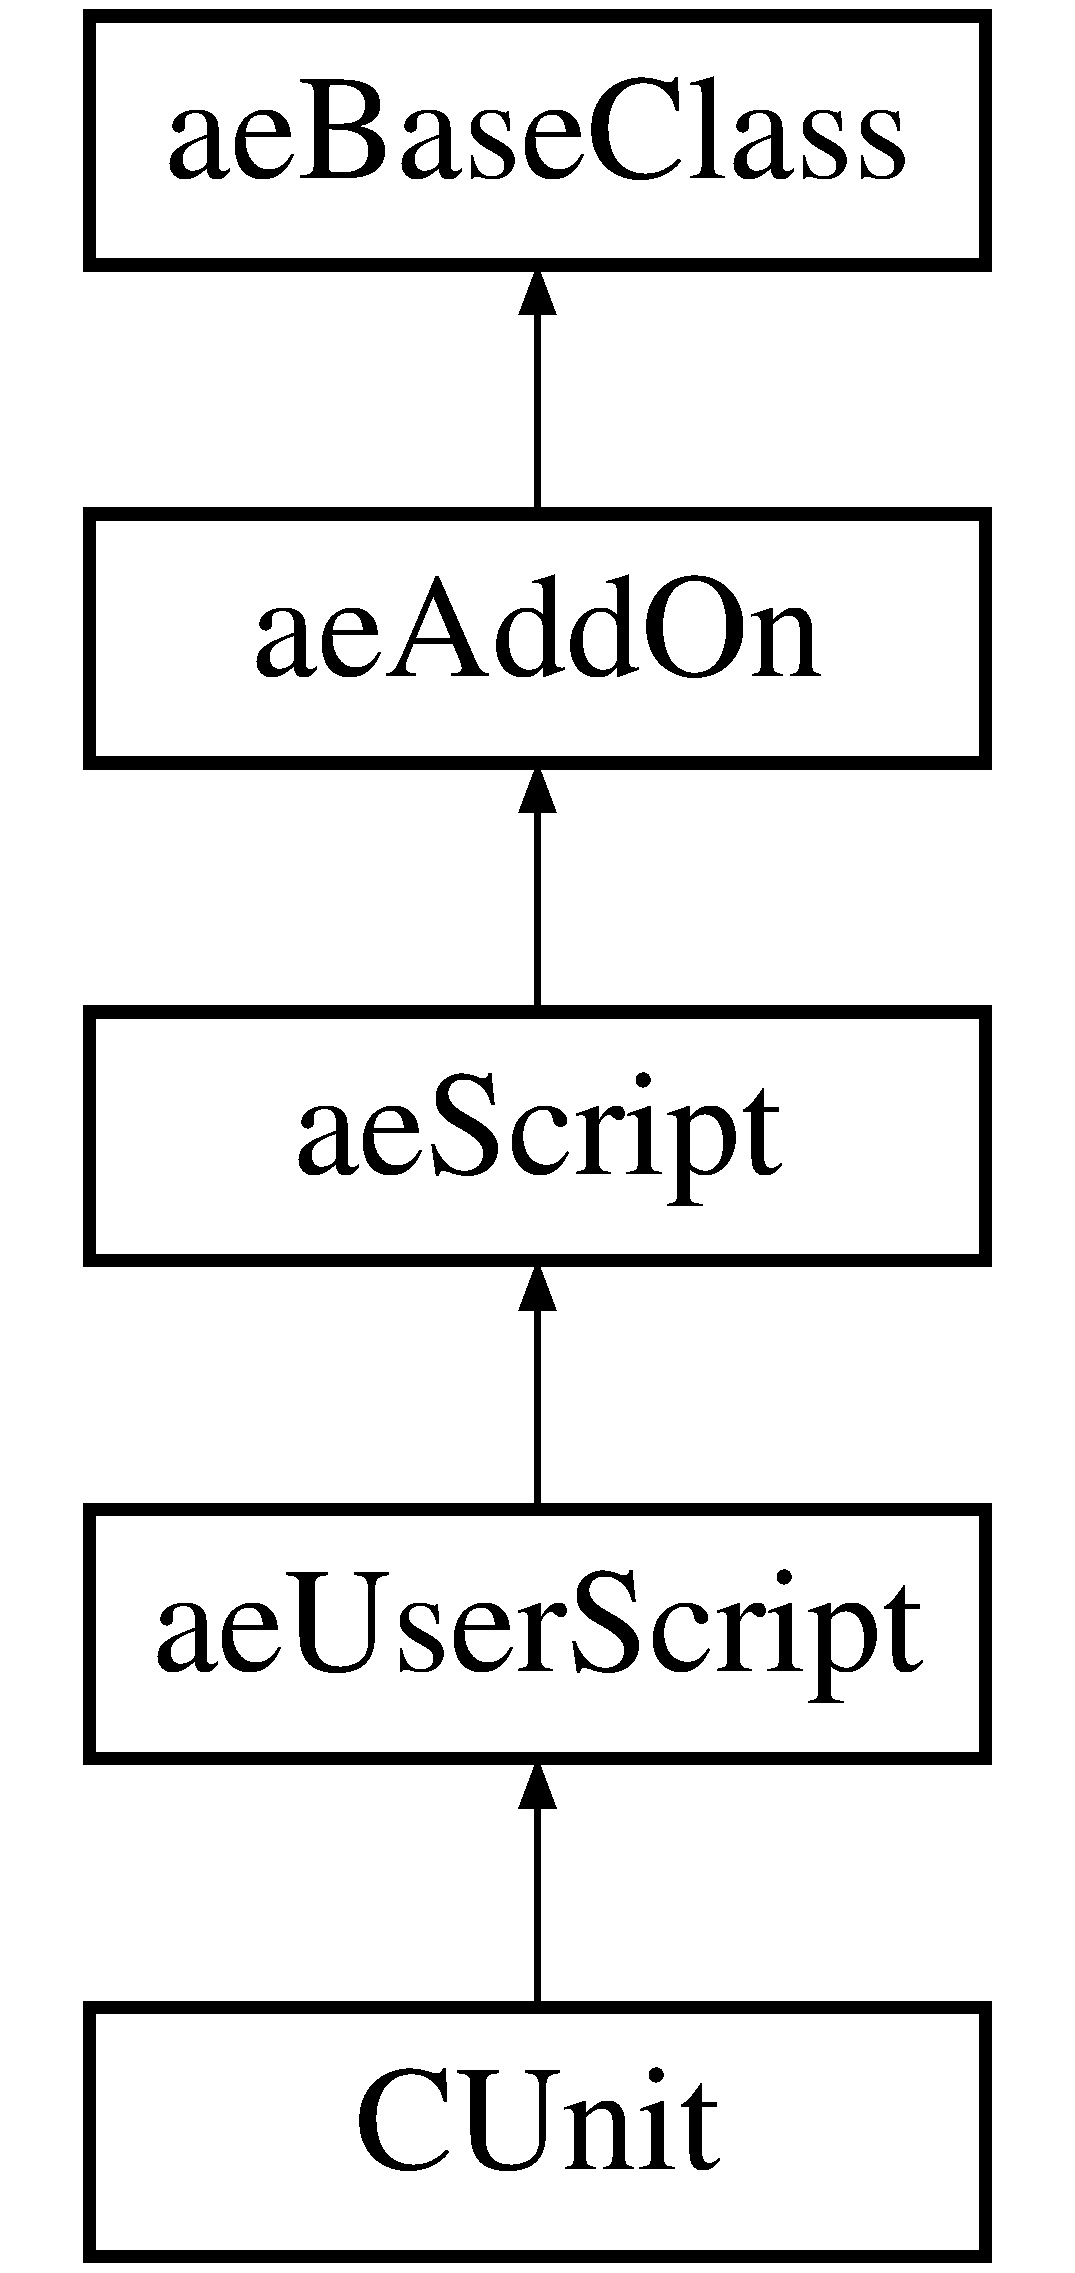
\includegraphics[height=5.000000cm]{class_c_unit}
\end{center}
\end{figure}
\subsection*{Public Member Functions}
\begin{DoxyCompactItemize}
\item 
int \hyperlink{class_c_unit_a092b74e62d924b87deead104dbc08e01}{Init} (\hyperlink{classae_base_class}{ae\+Base\+Class} $\ast$p\+Parent)
\begin{DoxyCompactList}\small\item\em Initializes with the given parent pointer. \end{DoxyCompactList}\item 
void \hyperlink{class_c_unit_a2514b846a8c131c1120e34f0ded85dbf}{Destroy} ()\hypertarget{class_c_unit_a2514b846a8c131c1120e34f0ded85dbf}{}\label{class_c_unit_a2514b846a8c131c1120e34f0ded85dbf}

\begin{DoxyCompactList}\small\item\em Destroys this object. \end{DoxyCompactList}\item 
void \hyperlink{class_c_unit_a5f46103027aaf83b2b47c0711640bd69}{Update} (float f\+Delta)
\begin{DoxyCompactList}\small\item\em Updates the given f\+Delta. \end{DoxyCompactList}\item 
void {\bfseries Move} (float f\+Delta)\hypertarget{class_c_unit_a4e77567811440d81879017d674e904e8}{}\label{class_c_unit_a4e77567811440d81879017d674e904e8}

\item 
void {\bfseries Get\+Hit} (float Damage)\hypertarget{class_c_unit_a434bb669567483c048cbfe66324f4335}{}\label{class_c_unit_a434bb669567483c048cbfe66324f4335}

\item 
void {\bfseries Set\+Units\+Around} (std\+::list$<$ \hyperlink{classae_game_object}{ae\+Game\+Object} $\ast$ $>$ $\ast$Game\+Objects)\hypertarget{class_c_unit_a1e91791fd7fafc99c57397d830361107}{}\label{class_c_unit_a1e91791fd7fafc99c57397d830361107}

\item 
std\+::vector$<$ \hyperlink{class_c_unit}{C\+Unit} $\ast$ $>$ $\ast$ {\bfseries Get\+Enemies\+Around} (float Range)\hypertarget{class_c_unit_aae47c49c723b853fa91d6eebf3fee383}{}\label{class_c_unit_aae47c49c723b853fa91d6eebf3fee383}

\item 
bool {\bfseries Can\+Attack} ()\hypertarget{class_c_unit_a5b2ba24542238e487709b97217bbe795}{}\label{class_c_unit_a5b2ba24542238e487709b97217bbe795}

\item 
bool {\bfseries Can\+Build} ()\hypertarget{class_c_unit_a7da13aa6c27ff5d58b8a3a0e09015399}{}\label{class_c_unit_a7da13aa6c27ff5d58b8a3a0e09015399}

\item 
bool {\bfseries Enemies\+Around} (float Range)\hypertarget{class_c_unit_a14f8774cd7b83229f5c42e011e21ed5b}{}\label{class_c_unit_a14f8774cd7b83229f5c42e011e21ed5b}

\item 
bool {\bfseries Is\+Alive} ()\hypertarget{class_c_unit_a30840ce3e2b06428cc0bf428abb7d93a}{}\label{class_c_unit_a30840ce3e2b06428cc0bf428abb7d93a}

\item 
bool {\bfseries In\+Range} ()\hypertarget{class_c_unit_adb0734a36b67cd52091826a59e42e727}{}\label{class_c_unit_adb0734a36b67cd52091826a59e42e727}

\item 
bool {\bfseries Can\+Hit} ()\hypertarget{class_c_unit_a5b6d95188479a7870f31693899bcc5fb}{}\label{class_c_unit_a5b6d95188479a7870f31693899bcc5fb}

\item 
bool {\bfseries In\+Range} (ae\+Vector2 Point)\hypertarget{class_c_unit_a03c20f26680053ed8a9c34259d795244}{}\label{class_c_unit_a03c20f26680053ed8a9c34259d795244}

\item 
float {\bfseries Distance} (\hyperlink{structae_core_1_1ae_vector2}{ae\+Vector2} Position)\hypertarget{class_c_unit_a7452044a1e387744d251ecc1ce4ae7d5}{}\label{class_c_unit_a7452044a1e387744d251ecc1ce4ae7d5}

\end{DoxyCompactItemize}
\subsection*{Public Attributes}
\begin{DoxyCompactItemize}
\item 
int {\bfseries m\+\_\+n\+Team\+\_\+\+ID}\hypertarget{class_c_unit_ad4179f0926726019c01d3fe5175f11a6}{}\label{class_c_unit_ad4179f0926726019c01d3fe5175f11a6}

\item 
int {\bfseries m\+\_\+n\+HP}\hypertarget{class_c_unit_a4571992ad0eead29b2756bbbc972329a}{}\label{class_c_unit_a4571992ad0eead29b2756bbbc972329a}

\item 
int {\bfseries m\+\_\+n\+Current\+State}\hypertarget{class_c_unit_a865ab7d150521795b4afc54c6a41bf15}{}\label{class_c_unit_a865ab7d150521795b4afc54c6a41bf15}

\item 
bool {\bfseries m\+\_\+b\+Can\+Hit}\hypertarget{class_c_unit_ad4b9588b1ece5becfd76c7d276217c0a}{}\label{class_c_unit_ad4b9588b1ece5becfd76c7d276217c0a}

\item 
bool {\bfseries m\+\_\+b\+Walking}\hypertarget{class_c_unit_a9b096857bfc004e99ed5e7a7dcf939ad}{}\label{class_c_unit_a9b096857bfc004e99ed5e7a7dcf939ad}

\item 
float {\bfseries m\+\_\+f\+Attack\+Timer}\hypertarget{class_c_unit_abc542bcc38ee093a145e2d555ba778d9}{}\label{class_c_unit_abc542bcc38ee093a145e2d555ba778d9}

\item 
float {\bfseries m\+\_\+f\+Curren\+Time}\hypertarget{class_c_unit_a06e062cd8ba920782c1d3d38faeb1041}{}\label{class_c_unit_a06e062cd8ba920782c1d3d38faeb1041}

\item 
\hyperlink{classae_unit_type}{ae\+Unit\+Type} $\ast$ {\bfseries m\+\_\+p\+Base\+Unit}\hypertarget{class_c_unit_ae6ac33646d5fbebf6e70c3cfe62b41b3}{}\label{class_c_unit_ae6ac33646d5fbebf6e70c3cfe62b41b3}

\item 
ae\+Vector2 {\bfseries m\+\_\+v\+Position}\hypertarget{class_c_unit_a02a240e69ca2066d828800756bca65fe}{}\label{class_c_unit_a02a240e69ca2066d828800756bca65fe}

\item 
ae\+Vector2 {\bfseries m\+\_\+v\+Direction}\hypertarget{class_c_unit_a5eb6ec8f7407795f890867cffc1d8b19}{}\label{class_c_unit_a5eb6ec8f7407795f890867cffc1d8b19}

\item 
ae\+Vector2 {\bfseries m\+\_\+v\+Destination}\hypertarget{class_c_unit_a2b1f832849cabe95c3df784a221e7159}{}\label{class_c_unit_a2b1f832849cabe95c3df784a221e7159}

\item 
std\+::vector$<$ \hyperlink{class_c_unit}{C\+Unit} $\ast$ $>$ {\bfseries m\+\_\+a\+Units}\hypertarget{class_c_unit_a9aaee699a591a993100a8fbf89d3cf42}{}\label{class_c_unit_a9aaee699a591a993100a8fbf89d3cf42}

\item 
std\+::vector$<$ \hyperlink{class_c_unit}{C\+Unit} $\ast$ $>$ {\bfseries m\+\_\+a\+Enemies}\hypertarget{class_c_unit_a8e4e45d2e21d84f007cad5a54abe104e}{}\label{class_c_unit_a8e4e45d2e21d84f007cad5a54abe104e}

\item 
std\+::vector$<$ \hyperlink{classae_state_machine}{ae\+State\+Machine} $\ast$ $>$ $\ast$ {\bfseries m\+\_\+p\+State\+Machines}\hypertarget{class_c_unit_a7817e8f9d69101be377cc11d4b5eb97e}{}\label{class_c_unit_a7817e8f9d69101be377cc11d4b5eb97e}

\item 
\hyperlink{class_c_animation_renderer}{C\+Animation\+Renderer} $\ast$ {\bfseries m\+\_\+p\+Renderer}\hypertarget{class_c_unit_a201bc2b6370b906d4f594aae06cf7ab7}{}\label{class_c_unit_a201bc2b6370b906d4f594aae06cf7ab7}

\item 
\hyperlink{class_c_unit}{C\+Unit} $\ast$ {\bfseries m\+\_\+p\+Enemy}\hypertarget{class_c_unit_a84e2aece711dc1f5f04f1192108c93fd}{}\label{class_c_unit_a84e2aece711dc1f5f04f1192108c93fd}

\item 
\hyperlink{class_c_unit}{C\+Unit} $\ast$ {\bfseries m\+\_\+p\+Friend}\hypertarget{class_c_unit_a53e15ad7257e6778dc28988d694628d6}{}\label{class_c_unit_a53e15ad7257e6778dc28988d694628d6}

\end{DoxyCompactItemize}
\subsection*{Additional Inherited Members}


\subsection{Member Function Documentation}
\index{C\+Unit@{C\+Unit}!Init@{Init}}
\index{Init@{Init}!C\+Unit@{C\+Unit}}
\subsubsection[{\texorpdfstring{Init(ae\+Base\+Class $\ast$p\+Parent)}{Init(aeBaseClass *pParent)}}]{\setlength{\rightskip}{0pt plus 5cm}int C\+Unit\+::\+Init (
\begin{DoxyParamCaption}
\item[{{\bf ae\+Base\+Class} $\ast$}]{p\+Parent}
\end{DoxyParamCaption}
)\hspace{0.3cm}{\ttfamily [virtual]}}\hypertarget{class_c_unit_a092b74e62d924b87deead104dbc08e01}{}\label{class_c_unit_a092b74e62d924b87deead104dbc08e01}


Initializes with the given parent pointer. 


\begin{DoxyParams}[1]{Parameters}
\mbox{\tt in,out}  & {\em p\+Parent} & If non-\/null, the parent pointer. \\
\hline
\end{DoxyParams}


Implements \hyperlink{classae_add_on_a0730c1446e548031f9a4e98435a54675}{ae\+Add\+On}.

\index{C\+Unit@{C\+Unit}!Update@{Update}}
\index{Update@{Update}!C\+Unit@{C\+Unit}}
\subsubsection[{\texorpdfstring{Update(float f\+Delta)}{Update(float fDelta)}}]{\setlength{\rightskip}{0pt plus 5cm}void C\+Unit\+::\+Update (
\begin{DoxyParamCaption}
\item[{float}]{f\+Delta}
\end{DoxyParamCaption}
)\hspace{0.3cm}{\ttfamily [virtual]}}\hypertarget{class_c_unit_a5f46103027aaf83b2b47c0711640bd69}{}\label{class_c_unit_a5f46103027aaf83b2b47c0711640bd69}


Updates the given f\+Delta. 


\begin{DoxyParams}{Parameters}
{\em f\+Delta} & The delta time. \\
\hline
\end{DoxyParams}


Implements \hyperlink{classae_add_on_a51caa4b8680206495ea671e71991e231}{ae\+Add\+On}.



The documentation for this class was generated from the following files\+:\begin{DoxyCompactItemize}
\item 
C\+:/\+Users/\+Alvaro Estrada/\+Documents/\+Visual Studio 2015/\+Projects/\+R\+T\+S\+\_\+\+A\+E/\+R\+T\+S\+\_\+\+A\+E/\+Game/Unit.\+h\item 
C\+:/\+Users/\+Alvaro Estrada/\+Documents/\+Visual Studio 2015/\+Projects/\+R\+T\+S\+\_\+\+A\+E/\+R\+T\+S\+\_\+\+A\+E/\+Game/Unit.\+cpp\end{DoxyCompactItemize}

\hypertarget{class_c_unit_state}{}\section{C\+Unit\+State Class Reference}
\label{class_c_unit_state}\index{C\+Unit\+State@{C\+Unit\+State}}
Inheritance diagram for C\+Unit\+State\+:\begin{figure}[H]
\begin{center}
\leavevmode
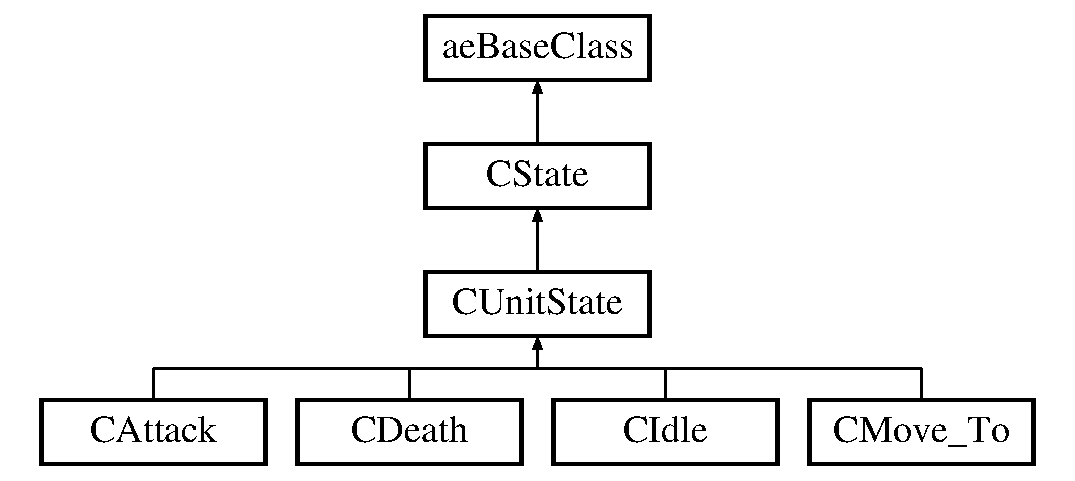
\includegraphics[height=4.000000cm]{class_c_unit_state}
\end{center}
\end{figure}
\subsection*{Additional Inherited Members}


The documentation for this class was generated from the following file\+:\begin{DoxyCompactItemize}
\item 
C\+:/\+Users/\+Alvaro Estrada/\+Documents/\+Visual Studio 2015/\+Projects/\+R\+T\+S\+\_\+\+A\+E/\+R\+T\+S\+\_\+\+A\+E/\+Game/Unit\+State.\+h\end{DoxyCompactItemize}

\hypertarget{class_c_unit_state_machine}{}\section{C\+Unit\+State\+Machine Class Reference}
\label{class_c_unit_state_machine}\index{C\+Unit\+State\+Machine@{C\+Unit\+State\+Machine}}
Inheritance diagram for C\+Unit\+State\+Machine\+:\begin{figure}[H]
\begin{center}
\leavevmode
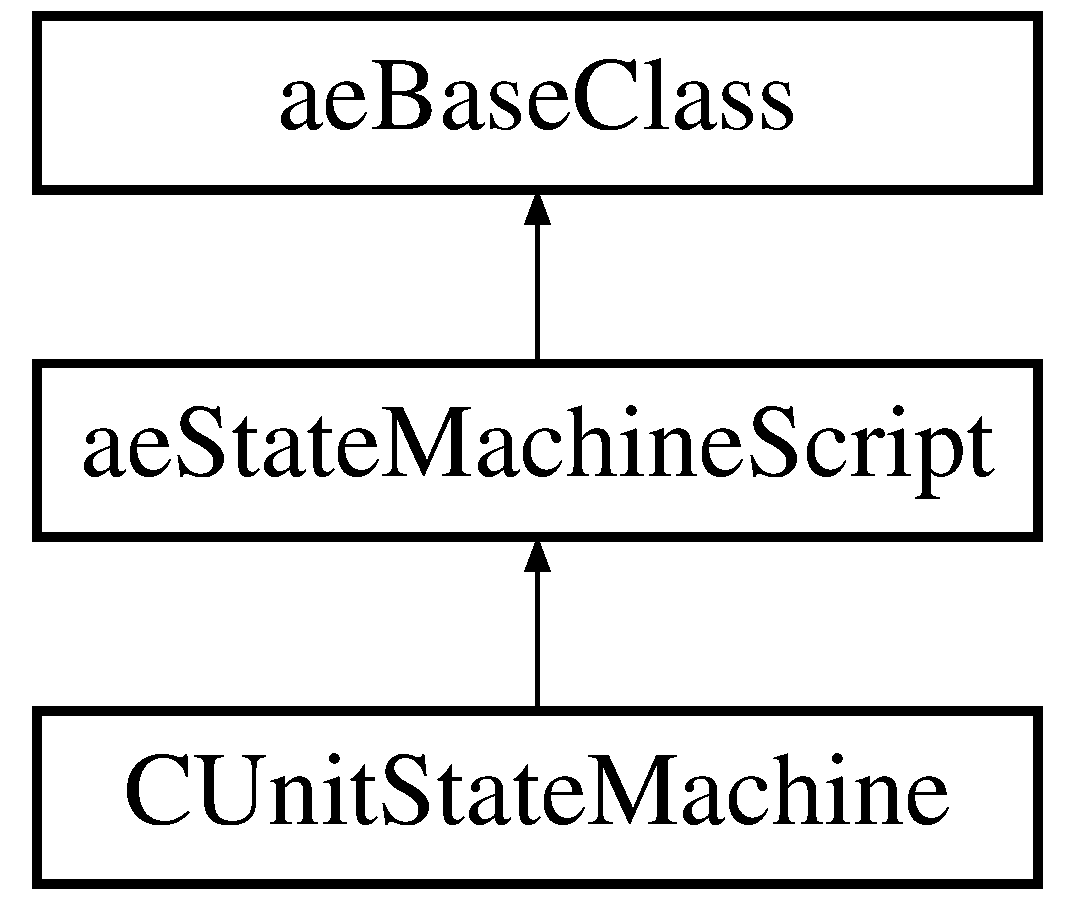
\includegraphics[height=3.000000cm]{class_c_unit_state_machine}
\end{center}
\end{figure}
\subsection*{Public Member Functions}
\begin{DoxyCompactItemize}
\item 
virtual void {\bfseries Set\+State} (int New\+State)\hypertarget{class_c_unit_state_machine_a5fb01eee64b2eb11bfced9a614b12173}{}\label{class_c_unit_state_machine_a5fb01eee64b2eb11bfced9a614b12173}

\end{DoxyCompactItemize}
\subsection*{Additional Inherited Members}


The documentation for this class was generated from the following files\+:\begin{DoxyCompactItemize}
\item 
C\+:/\+Users/\+Alvaro Estrada/\+Documents/\+Visual Studio 2015/\+Projects/\+R\+T\+S\+\_\+\+A\+E/\+R\+T\+S\+\_\+\+A\+E/\+Game/Unit\+State\+Machine.\+h\item 
C\+:/\+Users/\+Alvaro Estrada/\+Documents/\+Visual Studio 2015/\+Projects/\+R\+T\+S\+\_\+\+A\+E/\+R\+T\+S\+\_\+\+A\+E/\+Game/Unit\+State\+Machine.\+cpp\end{DoxyCompactItemize}

\hypertarget{structae_core_1_1ae_events_handler_1_1_event_compare}{}\section{ae\+Core\+:\+:ae\+Events\+Handler\+:\+:Event\+Compare Struct Reference}
\label{structae_core_1_1ae_events_handler_1_1_event_compare}\index{ae\+Core\+::ae\+Events\+Handler\+::\+Event\+Compare@{ae\+Core\+::ae\+Events\+Handler\+::\+Event\+Compare}}
\subsection*{Public Member Functions}
\begin{DoxyCompactItemize}
\item 
bool {\bfseries operator()} (const \hyperlink{structae_core_1_1ae_event}{ae\+Event} $\ast$t1, const \hyperlink{structae_core_1_1ae_event}{ae\+Event} $\ast$t2) const \hypertarget{structae_core_1_1ae_events_handler_1_1_event_compare_aa20b566bddab1abaaf5a253bac03eebe}{}\label{structae_core_1_1ae_events_handler_1_1_event_compare_aa20b566bddab1abaaf5a253bac03eebe}

\end{DoxyCompactItemize}


The documentation for this struct was generated from the following file\+:\begin{DoxyCompactItemize}
\item 
C\+:/\+Users/\+Alvaro Estrada/\+Documents/\+Visual Studio 2015/\+Projects/\+R\+T\+S\+\_\+\+A\+E/ae\+Core/\+Event\+System/Events\+System.\+h\end{DoxyCompactItemize}

\hypertarget{structae_a_star_path_finder_1_1_node_dist}{}\section{ae\+A\+Star\+Path\+Finder\+:\+:Node\+Dist Struct Reference}
\label{structae_a_star_path_finder_1_1_node_dist}\index{ae\+A\+Star\+Path\+Finder\+::\+Node\+Dist@{ae\+A\+Star\+Path\+Finder\+::\+Node\+Dist}}
\subsection*{Public Attributes}
\begin{DoxyCompactItemize}
\item 
\hyperlink{classae_a_star_map_tile_node}{ae\+A\+Star\+Map\+Tile\+Node} $\ast$ {\bfseries Node}\hypertarget{structae_a_star_path_finder_1_1_node_dist_a7bf8d0df285c6df55160aa188395d807}{}\label{structae_a_star_path_finder_1_1_node_dist_a7bf8d0df285c6df55160aa188395d807}

\item 
float {\bfseries Dist}\hypertarget{structae_a_star_path_finder_1_1_node_dist_a7ac0cb8ee4e1c7ee9170dc49db938b87}{}\label{structae_a_star_path_finder_1_1_node_dist_a7ac0cb8ee4e1c7ee9170dc49db938b87}

\end{DoxyCompactItemize}


The documentation for this struct was generated from the following file\+:\begin{DoxyCompactItemize}
\item 
C\+:/\+Users/\+Alvaro Estrada/\+Documents/\+Visual Studio 2015/\+Projects/\+R\+T\+S\+\_\+\+A\+E/\+R\+T\+S\+\_\+\+A\+E/\+Game/A\+Star.\+h\end{DoxyCompactItemize}

\hypertarget{structae_dijkstra_path_finder_1_1_node_dist}{}\section{ae\+Dijkstra\+Path\+Finder\+:\+:Node\+Dist Struct Reference}
\label{structae_dijkstra_path_finder_1_1_node_dist}\index{ae\+Dijkstra\+Path\+Finder\+::\+Node\+Dist@{ae\+Dijkstra\+Path\+Finder\+::\+Node\+Dist}}
\subsection*{Public Attributes}
\begin{DoxyCompactItemize}
\item 
\hyperlink{classae_map_tile_node}{ae\+Map\+Tile\+Node} $\ast$ {\bfseries Node}\hypertarget{structae_dijkstra_path_finder_1_1_node_dist_a8f100e40156613cc8f13c523457e7afb}{}\label{structae_dijkstra_path_finder_1_1_node_dist_a8f100e40156613cc8f13c523457e7afb}

\item 
int32 {\bfseries Dist}\hypertarget{structae_dijkstra_path_finder_1_1_node_dist_a2bf442c8b68dcca3a9066063779ab57b}{}\label{structae_dijkstra_path_finder_1_1_node_dist_a2bf442c8b68dcca3a9066063779ab57b}

\end{DoxyCompactItemize}


The documentation for this struct was generated from the following file\+:\begin{DoxyCompactItemize}
\item 
C\+:/\+Users/\+Alvaro Estrada/\+Documents/\+Visual Studio 2015/\+Projects/\+R\+T\+S\+\_\+\+A\+E/\+R\+T\+S\+\_\+\+A\+E/\+Game/Dijkstra.\+h\end{DoxyCompactItemize}

\hypertarget{structae_core_1_1ae_app_window_1_1_on_load}{}\section{ae\+Core\+:\+:ae\+App\+Window\+:\+:On\+Load Struct Reference}
\label{structae_core_1_1ae_app_window_1_1_on_load}\index{ae\+Core\+::ae\+App\+Window\+::\+On\+Load@{ae\+Core\+::ae\+App\+Window\+::\+On\+Load}}
\subsection*{Public Attributes}
\begin{DoxyCompactItemize}
\item 
\hyperlink{namespaceae_core_ad6f85aacc0d1fdd85e458e2413e60010}{ae\+String} {\bfseries psz\+Window\+Name}\hypertarget{structae_core_1_1ae_app_window_1_1_on_load_a6bd15124c3f00e80388d5c0f4f7e8bb2}{}\label{structae_core_1_1ae_app_window_1_1_on_load_a6bd15124c3f00e80388d5c0f4f7e8bb2}

\item 
\hyperlink{namespaceae_core_ad6f85aacc0d1fdd85e458e2413e60010}{ae\+String} {\bfseries psz\+Driver\+Name}\hypertarget{structae_core_1_1ae_app_window_1_1_on_load_aca6fd154c71472d582ed4fb46b391670}{}\label{structae_core_1_1ae_app_window_1_1_on_load_aca6fd154c71472d582ed4fb46b391670}

\item 
int {\bfseries X}\hypertarget{structae_core_1_1ae_app_window_1_1_on_load_a1571fd11d6e7c11da8c3f9d0e81231cc}{}\label{structae_core_1_1ae_app_window_1_1_on_load_a1571fd11d6e7c11da8c3f9d0e81231cc}

\item 
int {\bfseries Y}\hypertarget{structae_core_1_1ae_app_window_1_1_on_load_a7fd78c0b69e2726d7d1f130d8b712d4f}{}\label{structae_core_1_1ae_app_window_1_1_on_load_a7fd78c0b69e2726d7d1f130d8b712d4f}

\item 
int {\bfseries Width}\hypertarget{structae_core_1_1ae_app_window_1_1_on_load_adfd33a11ab0c73b4748a49e259ba3e54}{}\label{structae_core_1_1ae_app_window_1_1_on_load_adfd33a11ab0c73b4748a49e259ba3e54}

\item 
int {\bfseries Height}\hypertarget{structae_core_1_1ae_app_window_1_1_on_load_a2513febc473306a343e107a336d39ad7}{}\label{structae_core_1_1ae_app_window_1_1_on_load_a2513febc473306a343e107a336d39ad7}

\item 
int {\bfseries Window\+Flag}\hypertarget{structae_core_1_1ae_app_window_1_1_on_load_a3d96b003bfd35363e466b45fe2766258}{}\label{structae_core_1_1ae_app_window_1_1_on_load_a3d96b003bfd35363e466b45fe2766258}

\end{DoxyCompactItemize}


The documentation for this struct was generated from the following file\+:\begin{DoxyCompactItemize}
\item 
C\+:/\+Users/\+Alvaro Estrada/\+Documents/\+Visual Studio 2015/\+Projects/\+R\+T\+S\+\_\+\+A\+E/ae\+Core/\+Graphics/\hyperlink{_app_window_8h}{App\+Window.\+h}\end{DoxyCompactItemize}

\hypertarget{structae_a_star_path_finder_1_1_tile_compare}{}\section{ae\+A\+Star\+Path\+Finder\+:\+:Tile\+Compare Struct Reference}
\label{structae_a_star_path_finder_1_1_tile_compare}\index{ae\+A\+Star\+Path\+Finder\+::\+Tile\+Compare@{ae\+A\+Star\+Path\+Finder\+::\+Tile\+Compare}}
\subsection*{Public Member Functions}
\begin{DoxyCompactItemize}
\item 
bool {\bfseries operator()} (const \hyperlink{structae_a_star_path_finder_1_1_node_dist}{Node\+Dist} $\ast$t1, const \hyperlink{structae_a_star_path_finder_1_1_node_dist}{Node\+Dist} $\ast$t2) const \hypertarget{structae_a_star_path_finder_1_1_tile_compare_a19cbdc60ac92e3708282ff682ccb4d4e}{}\label{structae_a_star_path_finder_1_1_tile_compare_a19cbdc60ac92e3708282ff682ccb4d4e}

\end{DoxyCompactItemize}


The documentation for this struct was generated from the following file\+:\begin{DoxyCompactItemize}
\item 
C\+:/\+Users/\+Alvaro Estrada/\+Documents/\+Visual Studio 2015/\+Projects/\+R\+T\+S\+\_\+\+A\+E/\+R\+T\+S\+\_\+\+A\+E/\+Game/A\+Star.\+h\end{DoxyCompactItemize}

\hypertarget{structae_dijkstra_path_finder_1_1_tile_compare}{}\section{ae\+Dijkstra\+Path\+Finder\+:\+:Tile\+Compare Struct Reference}
\label{structae_dijkstra_path_finder_1_1_tile_compare}\index{ae\+Dijkstra\+Path\+Finder\+::\+Tile\+Compare@{ae\+Dijkstra\+Path\+Finder\+::\+Tile\+Compare}}
\subsection*{Public Member Functions}
\begin{DoxyCompactItemize}
\item 
bool {\bfseries operator()} (const \hyperlink{structae_dijkstra_path_finder_1_1_node_dist}{Node\+Dist} $\ast$t1, const \hyperlink{structae_dijkstra_path_finder_1_1_node_dist}{Node\+Dist} $\ast$t2) const \hypertarget{structae_dijkstra_path_finder_1_1_tile_compare_af62f9684bd29ed63bf1c3d1622cb2d82}{}\label{structae_dijkstra_path_finder_1_1_tile_compare_af62f9684bd29ed63bf1c3d1622cb2d82}

\end{DoxyCompactItemize}


The documentation for this struct was generated from the following file\+:\begin{DoxyCompactItemize}
\item 
C\+:/\+Users/\+Alvaro Estrada/\+Documents/\+Visual Studio 2015/\+Projects/\+R\+T\+S\+\_\+\+A\+E/\+R\+T\+S\+\_\+\+A\+E/\+Game/Dijkstra.\+h\end{DoxyCompactItemize}

\chapter{File Documentation}
\hypertarget{_app_window_8cpp}{}\section{C\+:/\+Users/\+Alvaro Estrada/\+Documents/\+Visual Studio 2015/\+Projects/\+R\+T\+S\+\_\+\+A\+E/ae\+Core/\+Graphics/\+App\+Window.cpp File Reference}
\label{_app_window_8cpp}\index{C\+:/\+Users/\+Alvaro Estrada/\+Documents/\+Visual Studio 2015/\+Projects/\+R\+T\+S\+\_\+\+A\+E/ae\+Core/\+Graphics/\+App\+Window.\+cpp@{C\+:/\+Users/\+Alvaro Estrada/\+Documents/\+Visual Studio 2015/\+Projects/\+R\+T\+S\+\_\+\+A\+E/ae\+Core/\+Graphics/\+App\+Window.\+cpp}}


Implements the application Windows Form.  


{\ttfamily \#include \char`\"{}ae\+Core\+Std.\+h\char`\"{}}\\*
{\ttfamily \#include \char`\"{}App\+Window.\+h\char`\"{}}\\*
\subsection*{Namespaces}
\begin{DoxyCompactItemize}
\item 
 \hyperlink{namespaceae_core}{ae\+Core}
\begin{DoxyCompactList}\small\item\em \end{DoxyCompactList}\end{DoxyCompactItemize}


\subsection{Detailed Description}
Implements the application Windows Form. 


\hypertarget{_app_window_8h}{}\section{C\+:/\+Users/\+Alvaro Estrada/\+Documents/\+Visual Studio 2015/\+Projects/\+R\+T\+S\+\_\+\+A\+E/ae\+Core/\+Graphics/\+App\+Window.h File Reference}
\label{_app_window_8h}\index{C\+:/\+Users/\+Alvaro Estrada/\+Documents/\+Visual Studio 2015/\+Projects/\+R\+T\+S\+\_\+\+A\+E/ae\+Core/\+Graphics/\+App\+Window.\+h@{C\+:/\+Users/\+Alvaro Estrada/\+Documents/\+Visual Studio 2015/\+Projects/\+R\+T\+S\+\_\+\+A\+E/ae\+Core/\+Graphics/\+App\+Window.\+h}}


Declares the application Windows Form.  


{\ttfamily \#include $<$Windows.\+h$>$}\\*
{\ttfamily \#include $<$S\+D\+L.\+h$>$}\\*
{\ttfamily \#include $<$S\+D\+L\+\_\+ttf.\+h$>$}\\*
{\ttfamily \#include $<$S\+D\+L\+\_\+image.\+h$>$}\\*
{\ttfamily \#include \char`\"{}Renderer.\+h\char`\"{}}\\*
{\ttfamily \#include \char`\"{}../\+Basic\+Classes.\+h\char`\"{}}\\*
\subsection*{Classes}
\begin{DoxyCompactItemize}
\item 
class \hyperlink{classae_core_1_1ae_app_window}{ae\+Core\+::ae\+App\+Window}
\begin{DoxyCompactList}\small\item\em This class purpose is to create a client window where the entire program will display. \end{DoxyCompactList}\item 
struct \hyperlink{structae_core_1_1ae_app_window_1_1_on_load}{ae\+Core\+::ae\+App\+Window\+::\+On\+Load}
\end{DoxyCompactItemize}
\subsection*{Namespaces}
\begin{DoxyCompactItemize}
\item 
 \hyperlink{namespaceae_core}{ae\+Core}
\begin{DoxyCompactList}\small\item\em \end{DoxyCompactList}\end{DoxyCompactItemize}
\subsection*{Enumerations}
\begin{DoxyCompactItemize}
\item 
enum \hyperlink{namespaceae_core_acdd369cfd195794193a8bd62815a642e}{ae\+Core\+::\+Window\+Flags} \+: uint16 \{ \\*
\hyperlink{namespaceae_core_acdd369cfd195794193a8bd62815a642eac7cb47fe75b31167b7d8135b6d3538e7}{ae\+Core\+::\+Window\+Flags\+::\+W\+I\+N\+D\+O\+W\+\_\+\+F\+U\+L\+L\+S\+C\+R\+E\+EN} = 0x00000001, 
\hyperlink{namespaceae_core_acdd369cfd195794193a8bd62815a642eadea4b20851100b7211bb456518feef46}{ae\+Core\+::\+Window\+Flags\+::\+W\+I\+N\+D\+O\+W\+\_\+\+O\+P\+E\+N\+GL} = 0x00000002, 
\hyperlink{namespaceae_core_acdd369cfd195794193a8bd62815a642ea63c0e4bb4dd1394771eb32f78d9118fd}{ae\+Core\+::\+Window\+Flags\+::\+W\+I\+N\+D\+O\+W\+\_\+\+S\+H\+O\+WN} = 0x00000004, 
\hyperlink{namespaceae_core_acdd369cfd195794193a8bd62815a642eabe3973126d0f7ab2871155232c60e694}{ae\+Core\+::\+Window\+Flags\+::\+W\+I\+N\+D\+O\+W\+\_\+\+H\+I\+D\+D\+EN} = 0x00000008, 
\\*
\hyperlink{namespaceae_core_acdd369cfd195794193a8bd62815a642ea280b7580def4664af4655b9cfd2eb79a}{ae\+Core\+::\+Window\+Flags\+::\+W\+I\+N\+D\+O\+W\+\_\+\+B\+O\+R\+D\+E\+R\+L\+E\+SS} = 0x00000010, 
\hyperlink{namespaceae_core_acdd369cfd195794193a8bd62815a642eafdc98c9638aa168e4127cd093f5fb669}{ae\+Core\+::\+Window\+Flags\+::\+W\+I\+N\+D\+O\+W\+\_\+\+R\+E\+S\+I\+Z\+A\+B\+LE} = 0x00000020, 
\hyperlink{namespaceae_core_acdd369cfd195794193a8bd62815a642ea4f5800351acfd91672d23ebdbf4cbf9c}{ae\+Core\+::\+Window\+Flags\+::\+W\+I\+N\+D\+O\+W\+\_\+\+M\+I\+N\+I\+M\+I\+Z\+ED} = 0x00000040, 
\hyperlink{namespaceae_core_acdd369cfd195794193a8bd62815a642eabd32d53c78346f06f176de017d99acce}{ae\+Core\+::\+Window\+Flags\+::\+W\+I\+N\+D\+O\+W\+\_\+\+M\+A\+X\+I\+M\+I\+Z\+ED} = 0x00000080, 
\\*
\hyperlink{namespaceae_core_acdd369cfd195794193a8bd62815a642eadc3ae5b884772002a35117f02d180002}{ae\+Core\+::\+Window\+Flags\+::\+W\+I\+N\+D\+O\+W\+\_\+\+I\+N\+P\+U\+T\+\_\+\+G\+R\+A\+B\+B\+ED} = 0x00000100, 
\hyperlink{namespaceae_core_acdd369cfd195794193a8bd62815a642ea7b28e867de277942e11b6f1714a4a204}{ae\+Core\+::\+Window\+Flags\+::\+W\+I\+N\+D\+O\+W\+\_\+\+I\+N\+P\+U\+T\+\_\+\+F\+O\+C\+US} = 0x00000200, 
\hyperlink{namespaceae_core_acdd369cfd195794193a8bd62815a642ea26c33004d772f01602c9a52433ba7b16}{ae\+Core\+::\+Window\+Flags\+::\+W\+I\+N\+D\+O\+W\+\_\+\+M\+O\+U\+S\+E\+\_\+\+F\+O\+C\+US} = 0x00000400, 
{\bfseries W\+I\+N\+D\+O\+W\+\_\+\+F\+U\+L\+L\+S\+C\+R\+E\+E\+N\+\_\+\+D\+E\+S\+K\+T\+OP} = (W\+I\+N\+D\+O\+W\+\_\+\+F\+U\+L\+L\+S\+C\+R\+E\+EN $\vert$ 0x00001000), 
\\*
\hyperlink{namespaceae_core_acdd369cfd195794193a8bd62815a642eae6c714d673eba7126eb3913a51fe847e}{ae\+Core\+::\+Window\+Flags\+::\+W\+I\+N\+D\+O\+W\+\_\+\+F\+O\+R\+E\+I\+GN} = 0x00000800, 
\hyperlink{namespaceae_core_acdd369cfd195794193a8bd62815a642ea3ec6e3bc70c8b497aa64c31b746081d4}{ae\+Core\+::\+Window\+Flags\+::\+W\+I\+N\+D\+O\+W\+\_\+\+A\+L\+L\+O\+W\+\_\+\+H\+I\+G\+H\+D\+PI} = 0x00002000, 
\hyperlink{namespaceae_core_acdd369cfd195794193a8bd62815a642eaad7e5439b9b863e32d197e9cebd53a30}{ae\+Core\+::\+Window\+Flags\+::\+W\+I\+N\+D\+O\+W\+\_\+\+M\+O\+U\+S\+E\+\_\+\+C\+A\+P\+T\+U\+RE} = 0x00004000
 \}
\end{DoxyCompactItemize}


\subsection{Detailed Description}
Declares the application Windows Form. 

\begin{DoxyAuthor}{Author}
Alvaro Estrada 
\end{DoxyAuthor}
\begin{DoxyDate}{Date}
14/05/2016 
\end{DoxyDate}

\hypertarget{_renderer_8h}{}\section{C\+:/\+Users/\+Alvaro Estrada/\+Documents/\+Visual Studio 2015/\+Projects/\+R\+T\+S\+\_\+\+A\+E/ae\+Core/\+Graphics/\+Renderer.h File Reference}
\label{_renderer_8h}\index{C\+:/\+Users/\+Alvaro Estrada/\+Documents/\+Visual Studio 2015/\+Projects/\+R\+T\+S\+\_\+\+A\+E/ae\+Core/\+Graphics/\+Renderer.\+h@{C\+:/\+Users/\+Alvaro Estrada/\+Documents/\+Visual Studio 2015/\+Projects/\+R\+T\+S\+\_\+\+A\+E/ae\+Core/\+Graphics/\+Renderer.\+h}}


Declares the renderer class.  


{\ttfamily \#include \char`\"{}App\+Window.\+h\char`\"{}}\\*
\subsection*{Classes}
\begin{DoxyCompactItemize}
\item 
class \hyperlink{classae_core_1_1ae_renderer}{ae\+Core\+::ae\+Renderer}
\begin{DoxyCompactList}\small\item\em Stores the window renderer so it can be passed along. \end{DoxyCompactList}\end{DoxyCompactItemize}
\subsection*{Namespaces}
\begin{DoxyCompactItemize}
\item 
 \hyperlink{namespaceae_core}{ae\+Core}
\begin{DoxyCompactList}\small\item\em \end{DoxyCompactList}\end{DoxyCompactItemize}


\subsection{Detailed Description}
Declares the renderer class. 


\hypertarget{_sprite_8cpp}{}\section{C\+:/\+Users/\+Alvaro Estrada/\+Documents/\+Visual Studio 2015/\+Projects/\+R\+T\+S\+\_\+\+A\+E/ae\+Core/\+Graphics/\+Sprite.cpp File Reference}
\label{_sprite_8cpp}\index{C\+:/\+Users/\+Alvaro Estrada/\+Documents/\+Visual Studio 2015/\+Projects/\+R\+T\+S\+\_\+\+A\+E/ae\+Core/\+Graphics/\+Sprite.\+cpp@{C\+:/\+Users/\+Alvaro Estrada/\+Documents/\+Visual Studio 2015/\+Projects/\+R\+T\+S\+\_\+\+A\+E/ae\+Core/\+Graphics/\+Sprite.\+cpp}}


Implements the sprite class.  


{\ttfamily \#include \char`\"{}ae\+Core\+Std.\+h\char`\"{}}\\*
{\ttfamily \#include \char`\"{}Sprite.\+h\char`\"{}}\\*
\subsection*{Namespaces}
\begin{DoxyCompactItemize}
\item 
 \hyperlink{namespaceae_core}{ae\+Core}
\begin{DoxyCompactList}\small\item\em \end{DoxyCompactList}\end{DoxyCompactItemize}


\subsection{Detailed Description}
Implements the sprite class. 


\hypertarget{_sprite_8h}{}\section{C\+:/\+Users/\+Alvaro Estrada/\+Documents/\+Visual Studio 2015/\+Projects/\+R\+T\+S\+\_\+\+A\+E/ae\+Core/\+Graphics/\+Sprite.h File Reference}
\label{_sprite_8h}\index{C\+:/\+Users/\+Alvaro Estrada/\+Documents/\+Visual Studio 2015/\+Projects/\+R\+T\+S\+\_\+\+A\+E/ae\+Core/\+Graphics/\+Sprite.\+h@{C\+:/\+Users/\+Alvaro Estrada/\+Documents/\+Visual Studio 2015/\+Projects/\+R\+T\+S\+\_\+\+A\+E/ae\+Core/\+Graphics/\+Sprite.\+h}}


Declares the sprite class.  


{\ttfamily \#include \char`\"{}Renderer.\+h\char`\"{}}\\*
\subsection*{Classes}
\begin{DoxyCompactItemize}
\item 
class \hyperlink{classae_core_1_1ae_font}{ae\+Core\+::ae\+Font}
\begin{DoxyCompactList}\small\item\em An ae font. \end{DoxyCompactList}\item 
class \hyperlink{classae_core_1_1ae_sprite}{ae\+Core\+::ae\+Sprite}
\begin{DoxyCompactList}\small\item\em This class reads and displays images given by the user. \end{DoxyCompactList}\end{DoxyCompactItemize}
\subsection*{Namespaces}
\begin{DoxyCompactItemize}
\item 
 \hyperlink{namespaceae_core}{ae\+Core}
\begin{DoxyCompactList}\small\item\em \end{DoxyCompactList}\end{DoxyCompactItemize}
\subsection*{Typedefs}
\begin{DoxyCompactItemize}
\item 
typedef std\+::vector$<$ \hyperlink{classae_core_1_1ae_sprite}{ae\+Core\+::ae\+Sprite} $\ast$ $>$ {\bfseries Sprite\+List}\hypertarget{_sprite_8h_a6dc3e3fb0a9a7e3d7a28bf0800874c83}{}\label{_sprite_8h_a6dc3e3fb0a9a7e3d7a28bf0800874c83}

\end{DoxyCompactItemize}


\subsection{Detailed Description}
Declares the sprite class. 


\hypertarget{_platform_math_8cpp}{}\section{C\+:/\+Users/\+Alvaro Estrada/\+Documents/\+Visual Studio 2015/\+Projects/\+R\+T\+S\+\_\+\+A\+E/ae\+Core/\+Math/\+Platform\+Math.cpp File Reference}
\label{_platform_math_8cpp}\index{C\+:/\+Users/\+Alvaro Estrada/\+Documents/\+Visual Studio 2015/\+Projects/\+R\+T\+S\+\_\+\+A\+E/ae\+Core/\+Math/\+Platform\+Math.\+cpp@{C\+:/\+Users/\+Alvaro Estrada/\+Documents/\+Visual Studio 2015/\+Projects/\+R\+T\+S\+\_\+\+A\+E/ae\+Core/\+Math/\+Platform\+Math.\+cpp}}


Implements the platform mathematics class.  


{\ttfamily \#include \char`\"{}ae\+Core\+Std.\+h\char`\"{}}\\*
{\ttfamily \#include \char`\"{}Platform\+Math.\+h\char`\"{}}\\*
\subsection*{Namespaces}
\begin{DoxyCompactItemize}
\item 
 \hyperlink{namespaceae_core}{ae\+Core}
\begin{DoxyCompactList}\small\item\em \end{DoxyCompactList}\end{DoxyCompactItemize}
\subsection*{Functions}
\begin{DoxyCompactItemize}
\item 
void \hyperlink{namespaceae_core_a2c863d5b4c10a1e2b3a082d21aa556d5}{ae\+Core\+::\+S\+Rand\+Init} (int32 Seed)
\begin{DoxyCompactList}\small\item\em Function to set the initial value of the seed. \end{DoxyCompactList}\item 
float \hyperlink{namespaceae_core_aefa36e8f9f0e8a5f96a3a08349ecaf33}{ae\+Core\+::\+S\+Rand} ()
\begin{DoxyCompactList}\small\item\em Generates a random float in the range from 0 to 1 using the S\+Rand\+Init seed. \end{DoxyCompactList}\item 
void \hyperlink{namespaceae_core_aa028dd1f50f9d79db1ccf58ddc64b729}{ae\+Core\+::\+Gauss\+Random\+Pair} (float \&result\+\_\+a, float \&result\+\_\+b, float d\+Mean, float d\+Std\+Deviation)
\begin{DoxyCompactList}\small\item\em Generates two random numbers using the polar form of the Box-\/\+Muller algorithm. \end{DoxyCompactList}\item 
float \hyperlink{namespaceae_core_a0d7dbd2dd241e6f9741502777fd5fb25}{ae\+Core\+::\+Gauss\+Random} (float d\+Mean, float d\+Std\+Deviation)
\begin{DoxyCompactList}\small\item\em Return one Gaussian random number. \end{DoxyCompactList}\item 
ae\+Point \hyperlink{namespaceae_core_a5134c200abd7d0125caf1f1d6258f78d}{ae\+Core\+::\+Get\+Map\+To\+Screen\+Coords} (ae\+Vector2 Point, ae\+Vector2 Camera\+Position, ae\+Rect Screen\+Precalc, bool Isometric)
\begin{DoxyCompactList}\small\item\em Gets map to screen coordinates. \end{DoxyCompactList}\item 
ae\+Vector2 \hyperlink{namespaceae_core_afe966a085ebb2ecbbb1953302ec3ed7e}{ae\+Core\+::\+Get\+Screen\+To\+Map\+Coords} (ae\+Point Point, ae\+Vector2 Camera\+Position, ae\+Rect Screen\+Precalc, bool Isometric)
\begin{DoxyCompactList}\small\item\em Gets screen to map coordinates. \end{DoxyCompactList}\end{DoxyCompactItemize}


\subsection{Detailed Description}
Implements the platform mathematics class. 


\hypertarget{_platform_math_8h}{}\section{C\+:/\+Users/\+Alvaro Estrada/\+Documents/\+Visual Studio 2015/\+Projects/\+R\+T\+S\+\_\+\+A\+E/ae\+Core/\+Math/\+Platform\+Math.h File Reference}
\label{_platform_math_8h}\index{C\+:/\+Users/\+Alvaro Estrada/\+Documents/\+Visual Studio 2015/\+Projects/\+R\+T\+S\+\_\+\+A\+E/ae\+Core/\+Math/\+Platform\+Math.\+h@{C\+:/\+Users/\+Alvaro Estrada/\+Documents/\+Visual Studio 2015/\+Projects/\+R\+T\+S\+\_\+\+A\+E/ae\+Core/\+Math/\+Platform\+Math.\+h}}


Declares the platform mathematics class.  


\subsection*{Namespaces}
\begin{DoxyCompactItemize}
\item 
 \hyperlink{namespaceae_core}{ae\+Core}
\begin{DoxyCompactList}\small\item\em \end{DoxyCompactList}\end{DoxyCompactItemize}
\subsection*{Macros}
\begin{DoxyCompactItemize}
\item 
\#define \hyperlink{_platform_math_8h_a598a3330b3c21701223ee0ca14316eca}{PI}~(3.\+1415926535897932f)
\item 
\#define \hyperlink{_platform_math_8h_a4b9c2c17b44d318829df5e1bd7e50f1d}{S\+M\+A\+L\+L\+\_\+\+N\+U\+M\+B\+ER}~(1.e-\/8f)
\item 
\#define \hyperlink{_platform_math_8h_a8c9f2aba435c6bee6a7b33104d08e44d}{K\+I\+N\+D\+A\+\_\+\+S\+M\+A\+L\+L\+\_\+\+N\+U\+M\+B\+ER}~(1.e-\/4f)
\item 
\#define \hyperlink{_platform_math_8h_a903291dbeb9127355bff6edc348567ca}{B\+I\+G\+\_\+\+N\+U\+M\+B\+ER}~(3.\+4e+38f)
\item 
\#define \hyperlink{_platform_math_8h_a4781887fe1e8f96649a2ca3cf37a9be4}{E\+U\+L\+E\+R\+S\+\_\+\+N\+U\+M\+B\+ER}~(2.\+71828182845904523536f)
\item 
\#define \hyperlink{_platform_math_8h_a58ce70c44358a600c06e31eb3be28b61}{M\+A\+X\+\_\+\+F\+LT}~3.\+402823466e+38F
\item 
\#define \hyperlink{_platform_math_8h_aebad45bfa06a5d66805c5813fbc59f4b}{I\+N\+V\+\_\+\+PI}~(0.\+31830988618f)
\item 
\#define \hyperlink{_platform_math_8h_ae3ec3219e4eee3b0992bfd59c2e2bc42}{H\+A\+L\+F\+\_\+\+PI}~(1.\+57079632679f)
\item 
\#define \hyperlink{_platform_math_8h_a3fd2b1bcd7ddcf506237987ad780f495}{D\+E\+L\+TA}~(0.\+00001f)
\item 
\#define {\bfseries F\+L\+O\+A\+T\+\_\+\+N\+O\+R\+M\+A\+L\+\_\+\+T\+H\+R\+E\+SH}~(0.\+0001f)\hypertarget{_platform_math_8h_a58e2669e9a8e24c6a32d2c0dc20d3a16}{}\label{_platform_math_8h_a58e2669e9a8e24c6a32d2c0dc20d3a16}

\item 
\#define \hyperlink{_platform_math_8h_a50f5a10542f73eb09dce32907c48a784}{T\+H\+R\+E\+S\+H\+\_\+\+P\+O\+I\+N\+T\+\_\+\+O\+N\+\_\+\+P\+L\+A\+NE}~(0.\+10f)
\item 
\#define \hyperlink{_platform_math_8h_a1b7b44de5dbcf5202a0017b12d3db6c0}{T\+H\+R\+E\+S\+H\+\_\+\+P\+O\+I\+N\+T\+\_\+\+O\+N\+\_\+\+S\+I\+DE}~(0.\+20f)
\item 
\#define \hyperlink{_platform_math_8h_a3ab44af3fd1761f42f182591b8116a08}{T\+H\+R\+E\+S\+H\+\_\+\+P\+O\+I\+N\+T\+S\+\_\+\+A\+R\+E\+\_\+\+S\+A\+ME}~(0.\+00002f)
\item 
\#define \hyperlink{_platform_math_8h_a4951547cba14143e6ccc7d543c0e2124}{T\+H\+R\+E\+S\+H\+\_\+\+P\+O\+I\+N\+T\+S\+\_\+\+A\+R\+E\+\_\+\+N\+E\+AR}~(0.\+015f)
\item 
\#define \hyperlink{_platform_math_8h_a430db886a2d3926e23d532693630a105}{T\+H\+R\+E\+S\+H\+\_\+\+N\+O\+R\+M\+A\+L\+S\+\_\+\+A\+R\+E\+\_\+\+S\+A\+ME}~(0.\+00002f)
\item 
\#define \hyperlink{_platform_math_8h_a2c880eb482e94f12adc0a9c9e33ee15e}{T\+H\+R\+E\+S\+H\+\_\+\+V\+E\+C\+T\+O\+R\+S\+\_\+\+A\+R\+E\+\_\+\+N\+E\+AR}~(0.\+0004f)
\item 
\#define \hyperlink{_platform_math_8h_a41594744f43b6d84567803a65e56e69c}{T\+H\+R\+E\+S\+H\+\_\+\+S\+P\+L\+I\+T\+\_\+\+P\+O\+L\+Y\+\_\+\+W\+I\+T\+H\+\_\+\+P\+L\+A\+NE}~(0.\+25f)
\item 
\#define \hyperlink{_platform_math_8h_a9a0cac5ca66563590e8ec0bdf75ec93c}{T\+H\+R\+E\+S\+H\+\_\+\+S\+P\+L\+I\+T\+\_\+\+P\+O\+L\+Y\+\_\+\+P\+R\+E\+C\+I\+S\+E\+LY}~(0.\+01f)
\item 
\#define \hyperlink{_platform_math_8h_af76eae9e6a977558e404ed6f4a34661e}{T\+H\+R\+E\+S\+H\+\_\+\+Z\+E\+R\+O\+\_\+\+N\+O\+R\+M\+\_\+\+S\+Q\+U\+A\+R\+ED}~(0.\+0001f)
\item 
\#define \hyperlink{_platform_math_8h_ad0c826cd625e4c14208b0997f0b00b8c}{T\+H\+R\+E\+S\+H\+\_\+\+V\+E\+C\+T\+O\+R\+S\+\_\+\+A\+R\+E\+\_\+\+P\+A\+R\+A\+L\+L\+EL}~(0.\+02f)
\item 
\#define {\bfseries R\+A\+N\+D\+O\+M\+\_\+\+C\+O\+N\+S\+T\+A\+N\+T\+\_\+A}~196314165\hypertarget{_platform_math_8h_a40dbfe3b9d427bf9a2af5f442df5e64d}{}\label{_platform_math_8h_a40dbfe3b9d427bf9a2af5f442df5e64d}

\item 
\#define {\bfseries R\+A\+N\+D\+O\+M\+\_\+\+C\+O\+N\+S\+T\+A\+N\+T\+\_\+B}~907633515\hypertarget{_platform_math_8h_a58a979a97ae5e8146269ab75ca6ad5e8}{}\label{_platform_math_8h_a58a979a97ae5e8146269ab75ca6ad5e8}

\end{DoxyCompactItemize}
\subsection*{Functions}
\begin{DoxyCompactItemize}
\item 
void \hyperlink{namespaceae_core_a2c863d5b4c10a1e2b3a082d21aa556d5}{ae\+Core\+::\+S\+Rand\+Init} (int32 Seed)
\begin{DoxyCompactList}\small\item\em Function to set the initial value of the seed. \end{DoxyCompactList}\item 
float \hyperlink{namespaceae_core_aefa36e8f9f0e8a5f96a3a08349ecaf33}{ae\+Core\+::\+S\+Rand} ()
\begin{DoxyCompactList}\small\item\em Generates a random float in the range from 0 to 1 using the S\+Rand\+Init seed. \end{DoxyCompactList}\item 
void \hyperlink{namespaceae_core_aa028dd1f50f9d79db1ccf58ddc64b729}{ae\+Core\+::\+Gauss\+Random\+Pair} (float \&result\+\_\+a, float \&result\+\_\+b, float d\+Mean, float d\+Std\+Deviation)
\begin{DoxyCompactList}\small\item\em Generates two random numbers using the polar form of the Box-\/\+Muller algorithm. \end{DoxyCompactList}\item 
float \hyperlink{namespaceae_core_a0d7dbd2dd241e6f9741502777fd5fb25}{ae\+Core\+::\+Gauss\+Random} (float d\+Mean, float d\+Std\+Deviation)
\begin{DoxyCompactList}\small\item\em Return one Gaussian random number. \end{DoxyCompactList}\item 
{\footnotesize template$<$$>$ }\\F\+O\+R\+C\+E\+I\+N\+L\+I\+NE float {\bfseries ae\+Core\+::\+Abs} (const float A)\hypertarget{namespaceae_core_aa3e9dbd69c1201c15eec5882f37750a7}{}\label{namespaceae_core_aa3e9dbd69c1201c15eec5882f37750a7}

\item 
ae\+Point \hyperlink{namespaceae_core_a5134c200abd7d0125caf1f1d6258f78d}{ae\+Core\+::\+Get\+Map\+To\+Screen\+Coords} (ae\+Vector2 Point, ae\+Vector2 Camera\+Position, ae\+Rect Screen\+Precalc, bool Isometric)
\begin{DoxyCompactList}\small\item\em Gets map to screen coordinates. \end{DoxyCompactList}\item 
ae\+Vector2 \hyperlink{namespaceae_core_afe966a085ebb2ecbbb1953302ec3ed7e}{ae\+Core\+::\+Get\+Screen\+To\+Map\+Coords} (ae\+Point Point, ae\+Vector2 Camera\+Position, ae\+Rect Screen\+Precalc, bool Isometric)
\begin{DoxyCompactList}\small\item\em Gets screen to map coordinates. \end{DoxyCompactList}\end{DoxyCompactItemize}


\subsection{Detailed Description}
Declares the platform mathematics class. 



\subsection{Macro Definition Documentation}
\index{Platform\+Math.\+h@{Platform\+Math.\+h}!B\+I\+G\+\_\+\+N\+U\+M\+B\+ER@{B\+I\+G\+\_\+\+N\+U\+M\+B\+ER}}
\index{B\+I\+G\+\_\+\+N\+U\+M\+B\+ER@{B\+I\+G\+\_\+\+N\+U\+M\+B\+ER}!Platform\+Math.\+h@{Platform\+Math.\+h}}
\subsubsection[{\texorpdfstring{B\+I\+G\+\_\+\+N\+U\+M\+B\+ER}{BIG_NUMBER}}]{\setlength{\rightskip}{0pt plus 5cm}\#define B\+I\+G\+\_\+\+N\+U\+M\+B\+ER~(3.\+4e+38f)}\hypertarget{_platform_math_8h_a903291dbeb9127355bff6edc348567ca}{}\label{_platform_math_8h_a903291dbeb9127355bff6edc348567ca}
\char`\"{}\+Big number\char`\"{} definition \index{Platform\+Math.\+h@{Platform\+Math.\+h}!D\+E\+L\+TA@{D\+E\+L\+TA}}
\index{D\+E\+L\+TA@{D\+E\+L\+TA}!Platform\+Math.\+h@{Platform\+Math.\+h}}
\subsubsection[{\texorpdfstring{D\+E\+L\+TA}{DELTA}}]{\setlength{\rightskip}{0pt plus 5cm}\#define D\+E\+L\+TA~(0.\+00001f)}\hypertarget{_platform_math_8h_a3fd2b1bcd7ddcf506237987ad780f495}{}\label{_platform_math_8h_a3fd2b1bcd7ddcf506237987ad780f495}
Magic number used for math precision \index{Platform\+Math.\+h@{Platform\+Math.\+h}!E\+U\+L\+E\+R\+S\+\_\+\+N\+U\+M\+B\+ER@{E\+U\+L\+E\+R\+S\+\_\+\+N\+U\+M\+B\+ER}}
\index{E\+U\+L\+E\+R\+S\+\_\+\+N\+U\+M\+B\+ER@{E\+U\+L\+E\+R\+S\+\_\+\+N\+U\+M\+B\+ER}!Platform\+Math.\+h@{Platform\+Math.\+h}}
\subsubsection[{\texorpdfstring{E\+U\+L\+E\+R\+S\+\_\+\+N\+U\+M\+B\+ER}{EULERS_NUMBER}}]{\setlength{\rightskip}{0pt plus 5cm}\#define E\+U\+L\+E\+R\+S\+\_\+\+N\+U\+M\+B\+ER~(2.\+71828182845904523536f)}\hypertarget{_platform_math_8h_a4781887fe1e8f96649a2ca3cf37a9be4}{}\label{_platform_math_8h_a4781887fe1e8f96649a2ca3cf37a9be4}
Euler�\+Mascheroni constant \index{Platform\+Math.\+h@{Platform\+Math.\+h}!H\+A\+L\+F\+\_\+\+PI@{H\+A\+L\+F\+\_\+\+PI}}
\index{H\+A\+L\+F\+\_\+\+PI@{H\+A\+L\+F\+\_\+\+PI}!Platform\+Math.\+h@{Platform\+Math.\+h}}
\subsubsection[{\texorpdfstring{H\+A\+L\+F\+\_\+\+PI}{HALF_PI}}]{\setlength{\rightskip}{0pt plus 5cm}\#define H\+A\+L\+F\+\_\+\+PI~(1.\+57079632679f)}\hypertarget{_platform_math_8h_ae3ec3219e4eee3b0992bfd59c2e2bc42}{}\label{_platform_math_8h_ae3ec3219e4eee3b0992bfd59c2e2bc42}
Half PI \index{Platform\+Math.\+h@{Platform\+Math.\+h}!I\+N\+V\+\_\+\+PI@{I\+N\+V\+\_\+\+PI}}
\index{I\+N\+V\+\_\+\+PI@{I\+N\+V\+\_\+\+PI}!Platform\+Math.\+h@{Platform\+Math.\+h}}
\subsubsection[{\texorpdfstring{I\+N\+V\+\_\+\+PI}{INV_PI}}]{\setlength{\rightskip}{0pt plus 5cm}\#define I\+N\+V\+\_\+\+PI~(0.\+31830988618f)}\hypertarget{_platform_math_8h_aebad45bfa06a5d66805c5813fbc59f4b}{}\label{_platform_math_8h_aebad45bfa06a5d66805c5813fbc59f4b}
Inverse of PI (1/\+PI) \index{Platform\+Math.\+h@{Platform\+Math.\+h}!K\+I\+N\+D\+A\+\_\+\+S\+M\+A\+L\+L\+\_\+\+N\+U\+M\+B\+ER@{K\+I\+N\+D\+A\+\_\+\+S\+M\+A\+L\+L\+\_\+\+N\+U\+M\+B\+ER}}
\index{K\+I\+N\+D\+A\+\_\+\+S\+M\+A\+L\+L\+\_\+\+N\+U\+M\+B\+ER@{K\+I\+N\+D\+A\+\_\+\+S\+M\+A\+L\+L\+\_\+\+N\+U\+M\+B\+ER}!Platform\+Math.\+h@{Platform\+Math.\+h}}
\subsubsection[{\texorpdfstring{K\+I\+N\+D\+A\+\_\+\+S\+M\+A\+L\+L\+\_\+\+N\+U\+M\+B\+ER}{KINDA_SMALL_NUMBER}}]{\setlength{\rightskip}{0pt plus 5cm}\#define K\+I\+N\+D\+A\+\_\+\+S\+M\+A\+L\+L\+\_\+\+N\+U\+M\+B\+ER~(1.e-\/4f)}\hypertarget{_platform_math_8h_a8c9f2aba435c6bee6a7b33104d08e44d}{}\label{_platform_math_8h_a8c9f2aba435c6bee6a7b33104d08e44d}
\char`\"{}\+Kinda small number\char`\"{} definition \index{Platform\+Math.\+h@{Platform\+Math.\+h}!M\+A\+X\+\_\+\+F\+LT@{M\+A\+X\+\_\+\+F\+LT}}
\index{M\+A\+X\+\_\+\+F\+LT@{M\+A\+X\+\_\+\+F\+LT}!Platform\+Math.\+h@{Platform\+Math.\+h}}
\subsubsection[{\texorpdfstring{M\+A\+X\+\_\+\+F\+LT}{MAX_FLT}}]{\setlength{\rightskip}{0pt plus 5cm}\#define M\+A\+X\+\_\+\+F\+LT~3.\+402823466e+38F}\hypertarget{_platform_math_8h_a58ce70c44358a600c06e31eb3be28b61}{}\label{_platform_math_8h_a58ce70c44358a600c06e31eb3be28b61}
Max value of a float (copy of float.\+h) \index{Platform\+Math.\+h@{Platform\+Math.\+h}!PI@{PI}}
\index{PI@{PI}!Platform\+Math.\+h@{Platform\+Math.\+h}}
\subsubsection[{\texorpdfstring{PI}{PI}}]{\setlength{\rightskip}{0pt plus 5cm}\#define PI~(3.\+1415926535897932f)}\hypertarget{_platform_math_8h_a598a3330b3c21701223ee0ca14316eca}{}\label{_platform_math_8h_a598a3330b3c21701223ee0ca14316eca}
PI constant \index{Platform\+Math.\+h@{Platform\+Math.\+h}!S\+M\+A\+L\+L\+\_\+\+N\+U\+M\+B\+ER@{S\+M\+A\+L\+L\+\_\+\+N\+U\+M\+B\+ER}}
\index{S\+M\+A\+L\+L\+\_\+\+N\+U\+M\+B\+ER@{S\+M\+A\+L\+L\+\_\+\+N\+U\+M\+B\+ER}!Platform\+Math.\+h@{Platform\+Math.\+h}}
\subsubsection[{\texorpdfstring{S\+M\+A\+L\+L\+\_\+\+N\+U\+M\+B\+ER}{SMALL_NUMBER}}]{\setlength{\rightskip}{0pt plus 5cm}\#define S\+M\+A\+L\+L\+\_\+\+N\+U\+M\+B\+ER~(1.e-\/8f)}\hypertarget{_platform_math_8h_a4b9c2c17b44d318829df5e1bd7e50f1d}{}\label{_platform_math_8h_a4b9c2c17b44d318829df5e1bd7e50f1d}
\char`\"{}\+Small number\char`\"{} definition \index{Platform\+Math.\+h@{Platform\+Math.\+h}!T\+H\+R\+E\+S\+H\+\_\+\+N\+O\+R\+M\+A\+L\+S\+\_\+\+A\+R\+E\+\_\+\+S\+A\+ME@{T\+H\+R\+E\+S\+H\+\_\+\+N\+O\+R\+M\+A\+L\+S\+\_\+\+A\+R\+E\+\_\+\+S\+A\+ME}}
\index{T\+H\+R\+E\+S\+H\+\_\+\+N\+O\+R\+M\+A\+L\+S\+\_\+\+A\+R\+E\+\_\+\+S\+A\+ME@{T\+H\+R\+E\+S\+H\+\_\+\+N\+O\+R\+M\+A\+L\+S\+\_\+\+A\+R\+E\+\_\+\+S\+A\+ME}!Platform\+Math.\+h@{Platform\+Math.\+h}}
\subsubsection[{\texorpdfstring{T\+H\+R\+E\+S\+H\+\_\+\+N\+O\+R\+M\+A\+L\+S\+\_\+\+A\+R\+E\+\_\+\+S\+A\+ME}{THRESH_NORMALS_ARE_SAME}}]{\setlength{\rightskip}{0pt plus 5cm}\#define T\+H\+R\+E\+S\+H\+\_\+\+N\+O\+R\+M\+A\+L\+S\+\_\+\+A\+R\+E\+\_\+\+S\+A\+ME~(0.\+00002f)}\hypertarget{_platform_math_8h_a430db886a2d3926e23d532693630a105}{}\label{_platform_math_8h_a430db886a2d3926e23d532693630a105}
Dos puntos normalizados son el mismo si est�n dentro de esta distancia (Hacer este n�mero muy grande resulta en clasificaci�n C\+SG incorrecta y en un desastre) \index{Platform\+Math.\+h@{Platform\+Math.\+h}!T\+H\+R\+E\+S\+H\+\_\+\+P\+O\+I\+N\+T\+\_\+\+O\+N\+\_\+\+P\+L\+A\+NE@{T\+H\+R\+E\+S\+H\+\_\+\+P\+O\+I\+N\+T\+\_\+\+O\+N\+\_\+\+P\+L\+A\+NE}}
\index{T\+H\+R\+E\+S\+H\+\_\+\+P\+O\+I\+N\+T\+\_\+\+O\+N\+\_\+\+P\+L\+A\+NE@{T\+H\+R\+E\+S\+H\+\_\+\+P\+O\+I\+N\+T\+\_\+\+O\+N\+\_\+\+P\+L\+A\+NE}!Platform\+Math.\+h@{Platform\+Math.\+h}}
\subsubsection[{\texorpdfstring{T\+H\+R\+E\+S\+H\+\_\+\+P\+O\+I\+N\+T\+\_\+\+O\+N\+\_\+\+P\+L\+A\+NE}{THRESH_POINT_ON_PLANE}}]{\setlength{\rightskip}{0pt plus 5cm}\#define T\+H\+R\+E\+S\+H\+\_\+\+P\+O\+I\+N\+T\+\_\+\+O\+N\+\_\+\+P\+L\+A\+NE~(0.\+10f)}\hypertarget{_platform_math_8h_a50f5a10542f73eb09dce32907c48a784}{}\label{_platform_math_8h_a50f5a10542f73eb09dce32907c48a784}
Thickness del plano para pruebas de front/back/inside \index{Platform\+Math.\+h@{Platform\+Math.\+h}!T\+H\+R\+E\+S\+H\+\_\+\+P\+O\+I\+N\+T\+\_\+\+O\+N\+\_\+\+S\+I\+DE@{T\+H\+R\+E\+S\+H\+\_\+\+P\+O\+I\+N\+T\+\_\+\+O\+N\+\_\+\+S\+I\+DE}}
\index{T\+H\+R\+E\+S\+H\+\_\+\+P\+O\+I\+N\+T\+\_\+\+O\+N\+\_\+\+S\+I\+DE@{T\+H\+R\+E\+S\+H\+\_\+\+P\+O\+I\+N\+T\+\_\+\+O\+N\+\_\+\+S\+I\+DE}!Platform\+Math.\+h@{Platform\+Math.\+h}}
\subsubsection[{\texorpdfstring{T\+H\+R\+E\+S\+H\+\_\+\+P\+O\+I\+N\+T\+\_\+\+O\+N\+\_\+\+S\+I\+DE}{THRESH_POINT_ON_SIDE}}]{\setlength{\rightskip}{0pt plus 5cm}\#define T\+H\+R\+E\+S\+H\+\_\+\+P\+O\+I\+N\+T\+\_\+\+O\+N\+\_\+\+S\+I\+DE~(0.\+20f)}\hypertarget{_platform_math_8h_a1b7b44de5dbcf5202a0017b12d3db6c0}{}\label{_platform_math_8h_a1b7b44de5dbcf5202a0017b12d3db6c0}
\char`\"{}\+Grosor\char`\"{} de los planos laterales de un pol�gono para pruebas point-\/inside/outside/on side \index{Platform\+Math.\+h@{Platform\+Math.\+h}!T\+H\+R\+E\+S\+H\+\_\+\+P\+O\+I\+N\+T\+S\+\_\+\+A\+R\+E\+\_\+\+N\+E\+AR@{T\+H\+R\+E\+S\+H\+\_\+\+P\+O\+I\+N\+T\+S\+\_\+\+A\+R\+E\+\_\+\+N\+E\+AR}}
\index{T\+H\+R\+E\+S\+H\+\_\+\+P\+O\+I\+N\+T\+S\+\_\+\+A\+R\+E\+\_\+\+N\+E\+AR@{T\+H\+R\+E\+S\+H\+\_\+\+P\+O\+I\+N\+T\+S\+\_\+\+A\+R\+E\+\_\+\+N\+E\+AR}!Platform\+Math.\+h@{Platform\+Math.\+h}}
\subsubsection[{\texorpdfstring{T\+H\+R\+E\+S\+H\+\_\+\+P\+O\+I\+N\+T\+S\+\_\+\+A\+R\+E\+\_\+\+N\+E\+AR}{THRESH_POINTS_ARE_NEAR}}]{\setlength{\rightskip}{0pt plus 5cm}\#define T\+H\+R\+E\+S\+H\+\_\+\+P\+O\+I\+N\+T\+S\+\_\+\+A\+R\+E\+\_\+\+N\+E\+AR~(0.\+015f)}\hypertarget{_platform_math_8h_a4951547cba14143e6ccc7d543c0e2124}{}\label{_platform_math_8h_a4951547cba14143e6ccc7d543c0e2124}
Dos puntos est�n cerca si est�n dentro de esta distancia y pueden ser convinados si la matem�tica imprecisa est� de acuerdo \index{Platform\+Math.\+h@{Platform\+Math.\+h}!T\+H\+R\+E\+S\+H\+\_\+\+P\+O\+I\+N\+T\+S\+\_\+\+A\+R\+E\+\_\+\+S\+A\+ME@{T\+H\+R\+E\+S\+H\+\_\+\+P\+O\+I\+N\+T\+S\+\_\+\+A\+R\+E\+\_\+\+S\+A\+ME}}
\index{T\+H\+R\+E\+S\+H\+\_\+\+P\+O\+I\+N\+T\+S\+\_\+\+A\+R\+E\+\_\+\+S\+A\+ME@{T\+H\+R\+E\+S\+H\+\_\+\+P\+O\+I\+N\+T\+S\+\_\+\+A\+R\+E\+\_\+\+S\+A\+ME}!Platform\+Math.\+h@{Platform\+Math.\+h}}
\subsubsection[{\texorpdfstring{T\+H\+R\+E\+S\+H\+\_\+\+P\+O\+I\+N\+T\+S\+\_\+\+A\+R\+E\+\_\+\+S\+A\+ME}{THRESH_POINTS_ARE_SAME}}]{\setlength{\rightskip}{0pt plus 5cm}\#define T\+H\+R\+E\+S\+H\+\_\+\+P\+O\+I\+N\+T\+S\+\_\+\+A\+R\+E\+\_\+\+S\+A\+ME~(0.\+00002f)}\hypertarget{_platform_math_8h_a3ab44af3fd1761f42f182591b8116a08}{}\label{_platform_math_8h_a3ab44af3fd1761f42f182591b8116a08}
Dos puntos son el mismo si est�n dentro de esta distancia \index{Platform\+Math.\+h@{Platform\+Math.\+h}!T\+H\+R\+E\+S\+H\+\_\+\+S\+P\+L\+I\+T\+\_\+\+P\+O\+L\+Y\+\_\+\+P\+R\+E\+C\+I\+S\+E\+LY@{T\+H\+R\+E\+S\+H\+\_\+\+S\+P\+L\+I\+T\+\_\+\+P\+O\+L\+Y\+\_\+\+P\+R\+E\+C\+I\+S\+E\+LY}}
\index{T\+H\+R\+E\+S\+H\+\_\+\+S\+P\+L\+I\+T\+\_\+\+P\+O\+L\+Y\+\_\+\+P\+R\+E\+C\+I\+S\+E\+LY@{T\+H\+R\+E\+S\+H\+\_\+\+S\+P\+L\+I\+T\+\_\+\+P\+O\+L\+Y\+\_\+\+P\+R\+E\+C\+I\+S\+E\+LY}!Platform\+Math.\+h@{Platform\+Math.\+h}}
\subsubsection[{\texorpdfstring{T\+H\+R\+E\+S\+H\+\_\+\+S\+P\+L\+I\+T\+\_\+\+P\+O\+L\+Y\+\_\+\+P\+R\+E\+C\+I\+S\+E\+LY}{THRESH_SPLIT_POLY_PRECISELY}}]{\setlength{\rightskip}{0pt plus 5cm}\#define T\+H\+R\+E\+S\+H\+\_\+\+S\+P\+L\+I\+T\+\_\+\+P\+O\+L\+Y\+\_\+\+P\+R\+E\+C\+I\+S\+E\+LY~(0.\+01f)}\hypertarget{_platform_math_8h_a9a0cac5ca66563590e8ec0bdf75ec93c}{}\label{_platform_math_8h_a9a0cac5ca66563590e8ec0bdf75ec93c}
Un plano divide exactamente por la mitad a un pol�gono \index{Platform\+Math.\+h@{Platform\+Math.\+h}!T\+H\+R\+E\+S\+H\+\_\+\+S\+P\+L\+I\+T\+\_\+\+P\+O\+L\+Y\+\_\+\+W\+I\+T\+H\+\_\+\+P\+L\+A\+NE@{T\+H\+R\+E\+S\+H\+\_\+\+S\+P\+L\+I\+T\+\_\+\+P\+O\+L\+Y\+\_\+\+W\+I\+T\+H\+\_\+\+P\+L\+A\+NE}}
\index{T\+H\+R\+E\+S\+H\+\_\+\+S\+P\+L\+I\+T\+\_\+\+P\+O\+L\+Y\+\_\+\+W\+I\+T\+H\+\_\+\+P\+L\+A\+NE@{T\+H\+R\+E\+S\+H\+\_\+\+S\+P\+L\+I\+T\+\_\+\+P\+O\+L\+Y\+\_\+\+W\+I\+T\+H\+\_\+\+P\+L\+A\+NE}!Platform\+Math.\+h@{Platform\+Math.\+h}}
\subsubsection[{\texorpdfstring{T\+H\+R\+E\+S\+H\+\_\+\+S\+P\+L\+I\+T\+\_\+\+P\+O\+L\+Y\+\_\+\+W\+I\+T\+H\+\_\+\+P\+L\+A\+NE}{THRESH_SPLIT_POLY_WITH_PLANE}}]{\setlength{\rightskip}{0pt plus 5cm}\#define T\+H\+R\+E\+S\+H\+\_\+\+S\+P\+L\+I\+T\+\_\+\+P\+O\+L\+Y\+\_\+\+W\+I\+T\+H\+\_\+\+P\+L\+A\+NE~(0.\+25f)}\hypertarget{_platform_math_8h_a41594744f43b6d84567803a65e56e69c}{}\label{_platform_math_8h_a41594744f43b6d84567803a65e56e69c}
Un plano divide a un pol�gono a la mitad \index{Platform\+Math.\+h@{Platform\+Math.\+h}!T\+H\+R\+E\+S\+H\+\_\+\+V\+E\+C\+T\+O\+R\+S\+\_\+\+A\+R\+E\+\_\+\+N\+E\+AR@{T\+H\+R\+E\+S\+H\+\_\+\+V\+E\+C\+T\+O\+R\+S\+\_\+\+A\+R\+E\+\_\+\+N\+E\+AR}}
\index{T\+H\+R\+E\+S\+H\+\_\+\+V\+E\+C\+T\+O\+R\+S\+\_\+\+A\+R\+E\+\_\+\+N\+E\+AR@{T\+H\+R\+E\+S\+H\+\_\+\+V\+E\+C\+T\+O\+R\+S\+\_\+\+A\+R\+E\+\_\+\+N\+E\+AR}!Platform\+Math.\+h@{Platform\+Math.\+h}}
\subsubsection[{\texorpdfstring{T\+H\+R\+E\+S\+H\+\_\+\+V\+E\+C\+T\+O\+R\+S\+\_\+\+A\+R\+E\+\_\+\+N\+E\+AR}{THRESH_VECTORS_ARE_NEAR}}]{\setlength{\rightskip}{0pt plus 5cm}\#define T\+H\+R\+E\+S\+H\+\_\+\+V\+E\+C\+T\+O\+R\+S\+\_\+\+A\+R\+E\+\_\+\+N\+E\+AR~(0.\+0004f)}\hypertarget{_platform_math_8h_a2c880eb482e94f12adc0a9c9e33ee15e}{}\label{_platform_math_8h_a2c880eb482e94f12adc0a9c9e33ee15e}
Dos vectores est�n cerca si est�n dentro de esta distancia y pueden ser convinados si la matem�tica imprecisa est� de acuerdo (Hacer este n�mero muy grande resulta en problemas de iluminaci�n debido a coordenadas de textura imprecisas) \index{Platform\+Math.\+h@{Platform\+Math.\+h}!T\+H\+R\+E\+S\+H\+\_\+\+V\+E\+C\+T\+O\+R\+S\+\_\+\+A\+R\+E\+\_\+\+P\+A\+R\+A\+L\+L\+EL@{T\+H\+R\+E\+S\+H\+\_\+\+V\+E\+C\+T\+O\+R\+S\+\_\+\+A\+R\+E\+\_\+\+P\+A\+R\+A\+L\+L\+EL}}
\index{T\+H\+R\+E\+S\+H\+\_\+\+V\+E\+C\+T\+O\+R\+S\+\_\+\+A\+R\+E\+\_\+\+P\+A\+R\+A\+L\+L\+EL@{T\+H\+R\+E\+S\+H\+\_\+\+V\+E\+C\+T\+O\+R\+S\+\_\+\+A\+R\+E\+\_\+\+P\+A\+R\+A\+L\+L\+EL}!Platform\+Math.\+h@{Platform\+Math.\+h}}
\subsubsection[{\texorpdfstring{T\+H\+R\+E\+S\+H\+\_\+\+V\+E\+C\+T\+O\+R\+S\+\_\+\+A\+R\+E\+\_\+\+P\+A\+R\+A\+L\+L\+EL}{THRESH_VECTORS_ARE_PARALLEL}}]{\setlength{\rightskip}{0pt plus 5cm}\#define T\+H\+R\+E\+S\+H\+\_\+\+V\+E\+C\+T\+O\+R\+S\+\_\+\+A\+R\+E\+\_\+\+P\+A\+R\+A\+L\+L\+EL~(0.\+02f)}\hypertarget{_platform_math_8h_ad0c826cd625e4c14208b0997f0b00b8c}{}\label{_platform_math_8h_ad0c826cd625e4c14208b0997f0b00b8c}
Los vectores son paralelos si el producto punto varia en menos que esto \index{Platform\+Math.\+h@{Platform\+Math.\+h}!T\+H\+R\+E\+S\+H\+\_\+\+Z\+E\+R\+O\+\_\+\+N\+O\+R\+M\+\_\+\+S\+Q\+U\+A\+R\+ED@{T\+H\+R\+E\+S\+H\+\_\+\+Z\+E\+R\+O\+\_\+\+N\+O\+R\+M\+\_\+\+S\+Q\+U\+A\+R\+ED}}
\index{T\+H\+R\+E\+S\+H\+\_\+\+Z\+E\+R\+O\+\_\+\+N\+O\+R\+M\+\_\+\+S\+Q\+U\+A\+R\+ED@{T\+H\+R\+E\+S\+H\+\_\+\+Z\+E\+R\+O\+\_\+\+N\+O\+R\+M\+\_\+\+S\+Q\+U\+A\+R\+ED}!Platform\+Math.\+h@{Platform\+Math.\+h}}
\subsubsection[{\texorpdfstring{T\+H\+R\+E\+S\+H\+\_\+\+Z\+E\+R\+O\+\_\+\+N\+O\+R\+M\+\_\+\+S\+Q\+U\+A\+R\+ED}{THRESH_ZERO_NORM_SQUARED}}]{\setlength{\rightskip}{0pt plus 5cm}\#define T\+H\+R\+E\+S\+H\+\_\+\+Z\+E\+R\+O\+\_\+\+N\+O\+R\+M\+\_\+\+S\+Q\+U\+A\+R\+ED~(0.\+0001f)}\hypertarget{_platform_math_8h_af76eae9e6a977558e404ed6f4a34661e}{}\label{_platform_math_8h_af76eae9e6a977558e404ed6f4a34661e}
Tama�o de una unidad normalizada que es considerada \char`\"{}zero\char`\"{} al cuadrado 
\hypertarget{_platform_definitions_8h}{}\section{C\+:/\+Users/\+Alvaro Estrada/\+Documents/\+Visual Studio 2015/\+Projects/\+R\+T\+S\+\_\+\+A\+E/ae\+Core/\+Platform\+Definitions.h File Reference}
\label{_platform_definitions_8h}\index{C\+:/\+Users/\+Alvaro Estrada/\+Documents/\+Visual Studio 2015/\+Projects/\+R\+T\+S\+\_\+\+A\+E/ae\+Core/\+Platform\+Definitions.\+h@{C\+:/\+Users/\+Alvaro Estrada/\+Documents/\+Visual Studio 2015/\+Projects/\+R\+T\+S\+\_\+\+A\+E/ae\+Core/\+Platform\+Definitions.\+h}}


Declares the platform definitions class.  


{\ttfamily \#include $<$string$>$}\\*
{\ttfamily \#include $<$vector$>$}\\*
{\ttfamily \#include $<$Windows.\+h$>$}\\*
\subsection*{Namespaces}
\begin{DoxyCompactItemize}
\item 
 \hyperlink{namespaceae_core}{ae\+Core}
\begin{DoxyCompactList}\small\item\em \end{DoxyCompactList}\end{DoxyCompactItemize}
\subsection*{Macros}
\begin{DoxyCompactItemize}
\item 
\#define {\bfseries A\+E\+\_\+\+N\+EW}~new\hypertarget{_platform_definitions_8h_ad17739ebb0dda7ac9e1ab418ca6d4d04}{}\label{_platform_definitions_8h_ad17739ebb0dda7ac9e1ab418ca6d4d04}

\item 
\#define {\bfseries A\+E\+\_\+\+D\+E\+L\+E\+TE}~delete\hypertarget{_platform_definitions_8h_a1a276b0d1caf7e0aaeb4ec958d6cd914}{}\label{_platform_definitions_8h_a1a276b0d1caf7e0aaeb4ec958d6cd914}

\item 
\#define {\bfseries A\+E\+\_\+\+D\+E\+L\+E\+T\+E\+\_\+\+A\+R\+R\+AY}~delete \mbox{[}$\,$\mbox{]}\hypertarget{_platform_definitions_8h_aaca30fb182eae0a9e544bc750656a13a}{}\label{_platform_definitions_8h_aaca30fb182eae0a9e544bc750656a13a}

\item 
\#define \hyperlink{_platform_definitions_8h_a4b8b2bed986c06c207ebac140ba65a7a}{S\+A\+F\+E\+\_\+\+D\+E\+L\+E\+TE}(x)~if(x) A\+E\+\_\+\+D\+E\+L\+E\+TE x; x=N\+U\+LL;
\begin{DoxyCompactList}\small\item\em A macro that defines safe delete. \end{DoxyCompactList}\item 
\#define \hyperlink{_platform_definitions_8h_a529602a5e4c2f9ba2c721ce9aefaddf7}{S\+A\+F\+E\+\_\+\+D\+E\+L\+E\+T\+E\+\_\+\+A\+R\+R\+AY}(x)~if (x) A\+E\+\_\+\+D\+E\+L\+E\+T\+E\+\_\+\+A\+R\+R\+AY x; x=N\+U\+LL;
\begin{DoxyCompactList}\small\item\em A macro that defines safe delete array. \end{DoxyCompactList}\item 
\#define \hyperlink{_platform_definitions_8h_a2bc549675ca29f733709b4656d22d52a}{S\+A\+F\+E\+\_\+\+R\+E\+L\+E\+A\+SE}(x)~if(x) x-\/$>$Release(); x=N\+U\+LL;
\begin{DoxyCompactList}\small\item\em A macro that defines safe release. \end{DoxyCompactList}\item 
\#define \hyperlink{_platform_definitions_8h_a469d1831fb34f756ff24a620c13569b7}{D\+L\+L\+\_\+\+C\+O\+N\+F\+IG}~\+\_\+declspec(dllimport)
\begin{DoxyCompactList}\small\item\em A macro that defines D\+LL configuration. \end{DoxyCompactList}\item 
\#define {\bfseries C\+O\+S\+\_\+\+P\+I\+\_\+\+Q\+U\+A\+R\+T\+ER}~0.\+707106f;\hypertarget{_platform_definitions_8h_a8b848ff8bdf624ab0b3d6eb1502bdb40}{}\label{_platform_definitions_8h_a8b848ff8bdf624ab0b3d6eb1502bdb40}

\item 
\#define {\bfseries P\+L\+A\+T\+F\+O\+R\+M\+\_\+\+T\+C\+H\+A\+R\+\_\+\+I\+S\+\_\+1\+\_\+\+B\+Y\+TE}~1\hypertarget{_platform_definitions_8h_aebae3c097b3a8ba61322087ac36824b9}{}\label{_platform_definitions_8h_aebae3c097b3a8ba61322087ac36824b9}

\end{DoxyCompactItemize}
\subsection*{Typedefs}
\begin{DoxyCompactItemize}
\item 
typedef unsigned char \hyperlink{namespaceae_core_aa13093dc911869e5b24942552898f01f}{ae\+Core\+::uint8}\hypertarget{namespaceae_core_aa13093dc911869e5b24942552898f01f}{}\label{namespaceae_core_aa13093dc911869e5b24942552898f01f}

\begin{DoxyCompactList}\small\item\em 8-\/bit unsigned. \end{DoxyCompactList}\item 
typedef unsigned short int \hyperlink{namespaceae_core_a1f9c426e6389a4ee13ee36ad25ec447d}{ae\+Core\+::uint16}\hypertarget{namespaceae_core_a1f9c426e6389a4ee13ee36ad25ec447d}{}\label{namespaceae_core_a1f9c426e6389a4ee13ee36ad25ec447d}

\begin{DoxyCompactList}\small\item\em 16-\/bit unsigned. \end{DoxyCompactList}\item 
typedef unsigned int \hyperlink{namespaceae_core_a7c60db1df33203b8e0e5e1db4129fa8d}{ae\+Core\+::uint32}\hypertarget{namespaceae_core_a7c60db1df33203b8e0e5e1db4129fa8d}{}\label{namespaceae_core_a7c60db1df33203b8e0e5e1db4129fa8d}

\begin{DoxyCompactList}\small\item\em 32-\/bit unsigned. \end{DoxyCompactList}\item 
typedef unsigned long long \hyperlink{namespaceae_core_a695dfc70e47466c7c04f8e058bd94fe9}{ae\+Core\+::uint64}\hypertarget{namespaceae_core_a695dfc70e47466c7c04f8e058bd94fe9}{}\label{namespaceae_core_a695dfc70e47466c7c04f8e058bd94fe9}

\begin{DoxyCompactList}\small\item\em 64-\/bit unsigned. \end{DoxyCompactList}\item 
typedef signed char \hyperlink{namespaceae_core_a91f573d8dc4c97ec3528c9d40720afd6}{ae\+Core\+::int8}\hypertarget{namespaceae_core_a91f573d8dc4c97ec3528c9d40720afd6}{}\label{namespaceae_core_a91f573d8dc4c97ec3528c9d40720afd6}

\begin{DoxyCompactList}\small\item\em 8-\/bit signed. \end{DoxyCompactList}\item 
typedef signed short int \hyperlink{namespaceae_core_ad0f2d0ae721a7f0afb159366dcc2da9c}{ae\+Core\+::int16}\hypertarget{namespaceae_core_ad0f2d0ae721a7f0afb159366dcc2da9c}{}\label{namespaceae_core_ad0f2d0ae721a7f0afb159366dcc2da9c}

\begin{DoxyCompactList}\small\item\em 16-\/bit signed. \end{DoxyCompactList}\item 
typedef signed int \hyperlink{namespaceae_core_a862bc39eb87cfabca273f49e2a920129}{ae\+Core\+::int32}\hypertarget{namespaceae_core_a862bc39eb87cfabca273f49e2a920129}{}\label{namespaceae_core_a862bc39eb87cfabca273f49e2a920129}

\begin{DoxyCompactList}\small\item\em 32-\/bit signed. \end{DoxyCompactList}\item 
typedef signed long long \hyperlink{namespaceae_core_aa97dc55535090f470938e38f4c1592b5}{ae\+Core\+::int64}\hypertarget{namespaceae_core_aa97dc55535090f470938e38f4c1592b5}{}\label{namespaceae_core_aa97dc55535090f470938e38f4c1592b5}

\begin{DoxyCompactList}\small\item\em 64-\/bit signed. \end{DoxyCompactList}\item 
typedef char \hyperlink{namespaceae_core_a33e0245ce11ed6c2fb08d03f342d07e6}{ae\+Core\+::\+A\+N\+S\+I\+C\+H\+AR}\hypertarget{namespaceae_core_a33e0245ce11ed6c2fb08d03f342d07e6}{}\label{namespaceae_core_a33e0245ce11ed6c2fb08d03f342d07e6}

\begin{DoxyCompactList}\small\item\em An A\+N\+SI char, normally signed. \end{DoxyCompactList}\item 
typedef wchar\+\_\+t \hyperlink{namespaceae_core_af3736ff30e300b0b87681b5e1d11d1fd}{ae\+Core\+::\+U\+N\+I\+C\+H\+AR}\hypertarget{namespaceae_core_af3736ff30e300b0b87681b5e1d11d1fd}{}\label{namespaceae_core_af3736ff30e300b0b87681b5e1d11d1fd}

\begin{DoxyCompactList}\small\item\em A U\+N\+I\+C\+O\+DE char, normally signed. \end{DoxyCompactList}\item 
typedef char \hyperlink{namespaceae_core_a052c557709e5ab43db521b23085fd916}{ae\+Core\+::\+T\+C\+H\+AR}\hypertarget{namespaceae_core_a052c557709e5ab43db521b23085fd916}{}\label{namespaceae_core_a052c557709e5ab43db521b23085fd916}

\begin{DoxyCompactList}\small\item\em Defines T\+C\+H\+AR as a wide char. \end{DoxyCompactList}\item 
typedef std\+::string \hyperlink{namespaceae_core_ad6f85aacc0d1fdd85e458e2413e60010}{ae\+Core\+::ae\+String}\hypertarget{namespaceae_core_ad6f85aacc0d1fdd85e458e2413e60010}{}\label{namespaceae_core_ad6f85aacc0d1fdd85e458e2413e60010}

\begin{DoxyCompactList}\small\item\em Defines the type ae\+String. \end{DoxyCompactList}\end{DoxyCompactItemize}


\subsection{Detailed Description}
Declares the platform definitions class. 



\subsection{Macro Definition Documentation}
\index{Platform\+Definitions.\+h@{Platform\+Definitions.\+h}!D\+L\+L\+\_\+\+C\+O\+N\+F\+IG@{D\+L\+L\+\_\+\+C\+O\+N\+F\+IG}}
\index{D\+L\+L\+\_\+\+C\+O\+N\+F\+IG@{D\+L\+L\+\_\+\+C\+O\+N\+F\+IG}!Platform\+Definitions.\+h@{Platform\+Definitions.\+h}}
\subsubsection[{\texorpdfstring{D\+L\+L\+\_\+\+C\+O\+N\+F\+IG}{DLL_CONFIG}}]{\setlength{\rightskip}{0pt plus 5cm}\#define D\+L\+L\+\_\+\+C\+O\+N\+F\+IG~\+\_\+declspec(dllimport)}\hypertarget{_platform_definitions_8h_a469d1831fb34f756ff24a620c13569b7}{}\label{_platform_definitions_8h_a469d1831fb34f756ff24a620c13569b7}


A macro that defines D\+LL configuration. 


\begin{DoxyParams}{Parameters}
{\em dllimport} & The dllimport. \\
\hline
\end{DoxyParams}
\index{Platform\+Definitions.\+h@{Platform\+Definitions.\+h}!S\+A\+F\+E\+\_\+\+D\+E\+L\+E\+TE@{S\+A\+F\+E\+\_\+\+D\+E\+L\+E\+TE}}
\index{S\+A\+F\+E\+\_\+\+D\+E\+L\+E\+TE@{S\+A\+F\+E\+\_\+\+D\+E\+L\+E\+TE}!Platform\+Definitions.\+h@{Platform\+Definitions.\+h}}
\subsubsection[{\texorpdfstring{S\+A\+F\+E\+\_\+\+D\+E\+L\+E\+TE}{SAFE_DELETE}}]{\setlength{\rightskip}{0pt plus 5cm}\#define S\+A\+F\+E\+\_\+\+D\+E\+L\+E\+TE(
\begin{DoxyParamCaption}
\item[{}]{x}
\end{DoxyParamCaption}
)~if(x) A\+E\+\_\+\+D\+E\+L\+E\+TE x; x=N\+U\+LL;}\hypertarget{_platform_definitions_8h_a4b8b2bed986c06c207ebac140ba65a7a}{}\label{_platform_definitions_8h_a4b8b2bed986c06c207ebac140ba65a7a}


A macro that defines safe delete. 


\begin{DoxyParams}{Parameters}
{\em x} & The void to process. \\
\hline
\end{DoxyParams}
\index{Platform\+Definitions.\+h@{Platform\+Definitions.\+h}!S\+A\+F\+E\+\_\+\+D\+E\+L\+E\+T\+E\+\_\+\+A\+R\+R\+AY@{S\+A\+F\+E\+\_\+\+D\+E\+L\+E\+T\+E\+\_\+\+A\+R\+R\+AY}}
\index{S\+A\+F\+E\+\_\+\+D\+E\+L\+E\+T\+E\+\_\+\+A\+R\+R\+AY@{S\+A\+F\+E\+\_\+\+D\+E\+L\+E\+T\+E\+\_\+\+A\+R\+R\+AY}!Platform\+Definitions.\+h@{Platform\+Definitions.\+h}}
\subsubsection[{\texorpdfstring{S\+A\+F\+E\+\_\+\+D\+E\+L\+E\+T\+E\+\_\+\+A\+R\+R\+AY}{SAFE_DELETE_ARRAY}}]{\setlength{\rightskip}{0pt plus 5cm}\#define S\+A\+F\+E\+\_\+\+D\+E\+L\+E\+T\+E\+\_\+\+A\+R\+R\+AY(
\begin{DoxyParamCaption}
\item[{}]{x}
\end{DoxyParamCaption}
)~if (x) A\+E\+\_\+\+D\+E\+L\+E\+T\+E\+\_\+\+A\+R\+R\+AY x; x=N\+U\+LL;}\hypertarget{_platform_definitions_8h_a529602a5e4c2f9ba2c721ce9aefaddf7}{}\label{_platform_definitions_8h_a529602a5e4c2f9ba2c721ce9aefaddf7}


A macro that defines safe delete array. 


\begin{DoxyParams}{Parameters}
{\em x} & The void to process. \\
\hline
\end{DoxyParams}
\index{Platform\+Definitions.\+h@{Platform\+Definitions.\+h}!S\+A\+F\+E\+\_\+\+R\+E\+L\+E\+A\+SE@{S\+A\+F\+E\+\_\+\+R\+E\+L\+E\+A\+SE}}
\index{S\+A\+F\+E\+\_\+\+R\+E\+L\+E\+A\+SE@{S\+A\+F\+E\+\_\+\+R\+E\+L\+E\+A\+SE}!Platform\+Definitions.\+h@{Platform\+Definitions.\+h}}
\subsubsection[{\texorpdfstring{S\+A\+F\+E\+\_\+\+R\+E\+L\+E\+A\+SE}{SAFE_RELEASE}}]{\setlength{\rightskip}{0pt plus 5cm}\#define S\+A\+F\+E\+\_\+\+R\+E\+L\+E\+A\+SE(
\begin{DoxyParamCaption}
\item[{}]{x}
\end{DoxyParamCaption}
)~if(x) x-\/$>$Release(); x=N\+U\+LL;}\hypertarget{_platform_definitions_8h_a2bc549675ca29f733709b4656d22d52a}{}\label{_platform_definitions_8h_a2bc549675ca29f733709b4656d22d52a}


A macro that defines safe release. 


\begin{DoxyParams}{Parameters}
{\em x} & The void to process. \\
\hline
\end{DoxyParams}

\hypertarget{_s_q_l_connector_8cpp}{}\section{C\+:/\+Users/\+Alvaro Estrada/\+Documents/\+Visual Studio 2015/\+Projects/\+R\+T\+S\+\_\+\+A\+E/ae\+Core/\+S\+Q\+L/\+S\+Q\+L\+Connector.cpp File Reference}
\label{_s_q_l_connector_8cpp}\index{C\+:/\+Users/\+Alvaro Estrada/\+Documents/\+Visual Studio 2015/\+Projects/\+R\+T\+S\+\_\+\+A\+E/ae\+Core/\+S\+Q\+L/\+S\+Q\+L\+Connector.\+cpp@{C\+:/\+Users/\+Alvaro Estrada/\+Documents/\+Visual Studio 2015/\+Projects/\+R\+T\+S\+\_\+\+A\+E/ae\+Core/\+S\+Q\+L/\+S\+Q\+L\+Connector.\+cpp}}


Implements the S\+QL connector class.  


{\ttfamily \#include \char`\"{}ae\+Core\+Std.\+h\char`\"{}}\\*
{\ttfamily \#include \char`\"{}S\+Q\+L\+Connector.\+h\char`\"{}}\\*
\subsection*{Namespaces}
\begin{DoxyCompactItemize}
\item 
 \hyperlink{namespaceae_core}{ae\+Core}
\begin{DoxyCompactList}\small\item\em \end{DoxyCompactList}\end{DoxyCompactItemize}


\subsection{Detailed Description}
Implements the S\+QL connector class. 


\hypertarget{_s_q_l_connector_8h}{}\section{C\+:/\+Users/\+Alvaro Estrada/\+Documents/\+Visual Studio 2015/\+Projects/\+R\+T\+S\+\_\+\+A\+E/ae\+Core/\+S\+Q\+L/\+S\+Q\+L\+Connector.h File Reference}
\label{_s_q_l_connector_8h}\index{C\+:/\+Users/\+Alvaro Estrada/\+Documents/\+Visual Studio 2015/\+Projects/\+R\+T\+S\+\_\+\+A\+E/ae\+Core/\+S\+Q\+L/\+S\+Q\+L\+Connector.\+h@{C\+:/\+Users/\+Alvaro Estrada/\+Documents/\+Visual Studio 2015/\+Projects/\+R\+T\+S\+\_\+\+A\+E/ae\+Core/\+S\+Q\+L/\+S\+Q\+L\+Connector.\+h}}


Declares the S\+QL connector class.  


{\ttfamily \#include $<$sqlite3.\+h$>$}\\*
{\ttfamily \#include $<$sstream$>$}\\*
{\ttfamily \#include \char`\"{}../\+Platform\+Definitions.\+h\char`\"{}}\\*
\subsection*{Classes}
\begin{DoxyCompactItemize}
\item 
class \hyperlink{classae_core_1_1ae_s_q_l_connector}{ae\+Core\+::ae\+S\+Q\+L\+Connector}
\begin{DoxyCompactList}\small\item\em A S\+QL connector. This class purpose is to create a connection to the database using S\+QL commands. \end{DoxyCompactList}\end{DoxyCompactItemize}
\subsection*{Namespaces}
\begin{DoxyCompactItemize}
\item 
 \hyperlink{namespaceae_core}{ae\+Core}
\begin{DoxyCompactList}\small\item\em \end{DoxyCompactList}\end{DoxyCompactItemize}


\subsection{Detailed Description}
Declares the S\+QL connector class. 


\hypertarget{_add_on_8h}{}\section{C\+:/\+Users/\+Alvaro Estrada/\+Documents/\+Visual Studio 2015/\+Projects/\+R\+T\+S\+\_\+\+A\+E/\+R\+T\+S\+\_\+\+A\+E/\+Game/\+Add\+On.h File Reference}
\label{_add_on_8h}\index{C\+:/\+Users/\+Alvaro Estrada/\+Documents/\+Visual Studio 2015/\+Projects/\+R\+T\+S\+\_\+\+A\+E/\+R\+T\+S\+\_\+\+A\+E/\+Game/\+Add\+On.\+h@{C\+:/\+Users/\+Alvaro Estrada/\+Documents/\+Visual Studio 2015/\+Projects/\+R\+T\+S\+\_\+\+A\+E/\+R\+T\+S\+\_\+\+A\+E/\+Game/\+Add\+On.\+h}}


Declares the add on class.  


{\ttfamily \#include \char`\"{}Base\+Class.\+h\char`\"{}}\\*
{\ttfamily \#include $<$Graphics/\+Sprite.\+h$>$}\\*
{\ttfamily \#include $<$vector$>$}\\*
\subsection*{Classes}
\begin{DoxyCompactItemize}
\item 
class \hyperlink{classae_add_on}{ae\+Add\+On}
\begin{DoxyCompactList}\small\item\em An add on. \end{DoxyCompactList}\end{DoxyCompactItemize}
\subsection*{Typedefs}
\begin{DoxyCompactItemize}
\item 
typedef std\+::vector$<$ \hyperlink{classae_add_on}{ae\+Add\+On} $\ast$ $>$ \hyperlink{_add_on_8h_a0f4072611b509766afe7bb36d570ac80}{ae\+Add\+Ons}\hypertarget{_add_on_8h_a0f4072611b509766afe7bb36d570ac80}{}\label{_add_on_8h_a0f4072611b509766afe7bb36d570ac80}

\begin{DoxyCompactList}\small\item\em Defines an alias representing the add ons vector. \end{DoxyCompactList}\end{DoxyCompactItemize}
\subsection*{Enumerations}
\begin{DoxyCompactItemize}
\item 
enum \hyperlink{_add_on_8h_a10abdd289149f0a510d47930d565b1ea}{Add\+On\+Id} \{ \hyperlink{_add_on_8h_a10abdd289149f0a510d47930d565b1eaaa83f1ca5ad00b39773d9e6a26b0e70b2}{Add\+On\+Id\+::\+Scripts} = 0
 \}\begin{DoxyCompactList}\small\item\em Values that represent add on identifiers. \end{DoxyCompactList}
\end{DoxyCompactItemize}


\subsection{Detailed Description}
Declares the add on class. 



\subsection{Enumeration Type Documentation}
\index{Add\+On.\+h@{Add\+On.\+h}!Add\+On\+Id@{Add\+On\+Id}}
\index{Add\+On\+Id@{Add\+On\+Id}!Add\+On.\+h@{Add\+On.\+h}}
\subsubsection[{\texorpdfstring{Add\+On\+Id}{AddOnId}}]{\setlength{\rightskip}{0pt plus 5cm}enum {\bf Add\+On\+Id}\hspace{0.3cm}{\ttfamily [strong]}}\hypertarget{_add_on_8h_a10abdd289149f0a510d47930d565b1ea}{}\label{_add_on_8h_a10abdd289149f0a510d47930d565b1ea}


Values that represent add on identifiers. 

\begin{Desc}
\item[Enumerator]\par
\begin{description}
\index{Scripts@{Scripts}!Add\+On.\+h@{Add\+On.\+h}}\index{Add\+On.\+h@{Add\+On.\+h}!Scripts@{Scripts}}\item[{\em 
Scripts\hypertarget{_add_on_8h_a10abdd289149f0a510d47930d565b1eaaa83f1ca5ad00b39773d9e6a26b0e70b2}{}\label{_add_on_8h_a10abdd289149f0a510d47930d565b1eaaa83f1ca5ad00b39773d9e6a26b0e70b2}
}]Script ID \end{description}
\end{Desc}

\hypertarget{_base_class_8h}{}\section{C\+:/\+Users/\+Alvaro Estrada/\+Documents/\+Visual Studio 2015/\+Projects/\+R\+T\+S\+\_\+\+A\+E/\+R\+T\+S\+\_\+\+A\+E/\+Game/\+Base\+Class.h File Reference}
\label{_base_class_8h}\index{C\+:/\+Users/\+Alvaro Estrada/\+Documents/\+Visual Studio 2015/\+Projects/\+R\+T\+S\+\_\+\+A\+E/\+R\+T\+S\+\_\+\+A\+E/\+Game/\+Base\+Class.\+h@{C\+:/\+Users/\+Alvaro Estrada/\+Documents/\+Visual Studio 2015/\+Projects/\+R\+T\+S\+\_\+\+A\+E/\+R\+T\+S\+\_\+\+A\+E/\+Game/\+Base\+Class.\+h}}


Declares the base class for the hereditary tree.  


{\ttfamily \#include $<$vector$>$}\\*
\subsection*{Classes}
\begin{DoxyCompactItemize}
\item 
class \hyperlink{classae_base_class}{ae\+Base\+Class}
\begin{DoxyCompactList}\small\item\em A base class. \end{DoxyCompactList}\end{DoxyCompactItemize}
\subsection*{Enumerations}
\begin{DoxyCompactItemize}
\item 
enum \hyperlink{_base_class_8h_aded8224779c70fab5084220935d672bb}{Class\+Id} \{ \\*
\hyperlink{_base_class_8h_aded8224779c70fab5084220935d672bba45b3e4c35409fb597ea598dc4b984b8c}{Class\+Id\+::\+Base\+Class} = 0, 
\hyperlink{_base_class_8h_aded8224779c70fab5084220935d672bbacdfd4357ab2cb8f241583cca76fcbb57}{Class\+Id\+::\+Preset}, 
\hyperlink{_base_class_8h_aded8224779c70fab5084220935d672bba3d164a4fbbdd103bddb596268f741bae}{Class\+Id\+::\+Game\+Object}, 
\hyperlink{_base_class_8h_aded8224779c70fab5084220935d672bba8f58d3c526622e5844b982e423c4351b}{Class\+Id\+::\+Add\+On}, 
\\*
\hyperlink{_base_class_8h_aded8224779c70fab5084220935d672bbae33d8b3de97b8246976dde33ff4abd48}{Class\+Id\+::\+State\+Machine}, 
\hyperlink{_base_class_8h_aded8224779c70fab5084220935d672bba3e7d9ec451bbfb4ef9ace4335280cdba}{Class\+Id\+::\+State\+Machine\+Script}, 
\hyperlink{_base_class_8h_aded8224779c70fab5084220935d672bba46a2a41cc6e552044816a2d04634545d}{Class\+Id\+::\+State}, 
\hyperlink{_base_class_8h_aded8224779c70fab5084220935d672bba1e3042b2e2a5550b412b37edd1c36b34}{Class\+Id\+::\+G\+UI}, 
\\*
\hyperlink{_base_class_8h_aded8224779c70fab5084220935d672bbaa191984d13955c955c48d8e2aefc19df}{Class\+Id\+::\+G\+U\+I\+Object}
 \}
\end{DoxyCompactItemize}


\subsection{Detailed Description}
Declares the base class for the hereditary tree. 



\subsection{Enumeration Type Documentation}
\index{Base\+Class.\+h@{Base\+Class.\+h}!Class\+Id@{Class\+Id}}
\index{Class\+Id@{Class\+Id}!Base\+Class.\+h@{Base\+Class.\+h}}
\subsubsection[{\texorpdfstring{Class\+Id}{ClassId}}]{\setlength{\rightskip}{0pt plus 5cm}enum {\bf Class\+Id}\hspace{0.3cm}{\ttfamily [strong]}}\hypertarget{_base_class_8h_aded8224779c70fab5084220935d672bb}{}\label{_base_class_8h_aded8224779c70fab5084220935d672bb}
\begin{Desc}
\item[Enumerator]\par
\begin{description}
\index{Base\+Class@{Base\+Class}!Base\+Class.\+h@{Base\+Class.\+h}}\index{Base\+Class.\+h@{Base\+Class.\+h}!Base\+Class@{Base\+Class}}\item[{\em 
Base\+Class\hypertarget{_base_class_8h_aded8224779c70fab5084220935d672bba45b3e4c35409fb597ea598dc4b984b8c}{}\label{_base_class_8h_aded8224779c70fab5084220935d672bba45b3e4c35409fb597ea598dc4b984b8c}
}]Basic class ID \index{Preset@{Preset}!Base\+Class.\+h@{Base\+Class.\+h}}\index{Base\+Class.\+h@{Base\+Class.\+h}!Preset@{Preset}}\item[{\em 
Preset\hypertarget{_base_class_8h_aded8224779c70fab5084220935d672bbacdfd4357ab2cb8f241583cca76fcbb57}{}\label{_base_class_8h_aded8224779c70fab5084220935d672bbacdfd4357ab2cb8f241583cca76fcbb57}
}]Preset ID \index{Game\+Object@{Game\+Object}!Base\+Class.\+h@{Base\+Class.\+h}}\index{Base\+Class.\+h@{Base\+Class.\+h}!Game\+Object@{Game\+Object}}\item[{\em 
Game\+Object\hypertarget{_base_class_8h_aded8224779c70fab5084220935d672bba3d164a4fbbdd103bddb596268f741bae}{}\label{_base_class_8h_aded8224779c70fab5084220935d672bba3d164a4fbbdd103bddb596268f741bae}
}]Game Object ID \index{Add\+On@{Add\+On}!Base\+Class.\+h@{Base\+Class.\+h}}\index{Base\+Class.\+h@{Base\+Class.\+h}!Add\+On@{Add\+On}}\item[{\em 
Add\+On\hypertarget{_base_class_8h_aded8224779c70fab5084220935d672bba8f58d3c526622e5844b982e423c4351b}{}\label{_base_class_8h_aded8224779c70fab5084220935d672bba8f58d3c526622e5844b982e423c4351b}
}]Add On ID \index{State\+Machine@{State\+Machine}!Base\+Class.\+h@{Base\+Class.\+h}}\index{Base\+Class.\+h@{Base\+Class.\+h}!State\+Machine@{State\+Machine}}\item[{\em 
State\+Machine\hypertarget{_base_class_8h_aded8224779c70fab5084220935d672bbae33d8b3de97b8246976dde33ff4abd48}{}\label{_base_class_8h_aded8224779c70fab5084220935d672bbae33d8b3de97b8246976dde33ff4abd48}
}]State machine ID \index{State\+Machine\+Script@{State\+Machine\+Script}!Base\+Class.\+h@{Base\+Class.\+h}}\index{Base\+Class.\+h@{Base\+Class.\+h}!State\+Machine\+Script@{State\+Machine\+Script}}\item[{\em 
State\+Machine\+Script\hypertarget{_base_class_8h_aded8224779c70fab5084220935d672bba3e7d9ec451bbfb4ef9ace4335280cdba}{}\label{_base_class_8h_aded8224779c70fab5084220935d672bba3e7d9ec451bbfb4ef9ace4335280cdba}
}]State machine script ID \index{State@{State}!Base\+Class.\+h@{Base\+Class.\+h}}\index{Base\+Class.\+h@{Base\+Class.\+h}!State@{State}}\item[{\em 
State\hypertarget{_base_class_8h_aded8224779c70fab5084220935d672bba46a2a41cc6e552044816a2d04634545d}{}\label{_base_class_8h_aded8224779c70fab5084220935d672bba46a2a41cc6e552044816a2d04634545d}
}]State ID \index{G\+UI@{G\+UI}!Base\+Class.\+h@{Base\+Class.\+h}}\index{Base\+Class.\+h@{Base\+Class.\+h}!G\+UI@{G\+UI}}\item[{\em 
G\+UI\hypertarget{_base_class_8h_aded8224779c70fab5084220935d672bba1e3042b2e2a5550b412b37edd1c36b34}{}\label{_base_class_8h_aded8224779c70fab5084220935d672bba1e3042b2e2a5550b412b37edd1c36b34}
}]G\+UI ID \index{G\+U\+I\+Object@{G\+U\+I\+Object}!Base\+Class.\+h@{Base\+Class.\+h}}\index{Base\+Class.\+h@{Base\+Class.\+h}!G\+U\+I\+Object@{G\+U\+I\+Object}}\item[{\em 
G\+U\+I\+Object\hypertarget{_base_class_8h_aded8224779c70fab5084220935d672bbaa191984d13955c955c48d8e2aefc19df}{}\label{_base_class_8h_aded8224779c70fab5084220935d672bbaa191984d13955c955c48d8e2aefc19df}
}]G\+UI Object ID \end{description}
\end{Desc}

\hypertarget{_breadth_first_search_8cpp}{}\section{C\+:/\+Users/\+Alvaro Estrada/\+Documents/\+Visual Studio 2015/\+Projects/\+R\+T\+S\+\_\+\+A\+E/\+R\+T\+S\+\_\+\+A\+E/\+Game/\+Breadth\+First\+Search.cpp File Reference}
\label{_breadth_first_search_8cpp}\index{C\+:/\+Users/\+Alvaro Estrada/\+Documents/\+Visual Studio 2015/\+Projects/\+R\+T\+S\+\_\+\+A\+E/\+R\+T\+S\+\_\+\+A\+E/\+Game/\+Breadth\+First\+Search.\+cpp@{C\+:/\+Users/\+Alvaro Estrada/\+Documents/\+Visual Studio 2015/\+Projects/\+R\+T\+S\+\_\+\+A\+E/\+R\+T\+S\+\_\+\+A\+E/\+Game/\+Breadth\+First\+Search.\+cpp}}


Implements the breadth first search path finder class.  


{\ttfamily \#include \char`\"{}stdafx.\+h\char`\"{}}\\*
{\ttfamily \#include \char`\"{}Breadth\+First\+Search.\+h\char`\"{}}\\*


\subsection{Detailed Description}
Implements the breadth first search path finder class. 


\hypertarget{_breadth_first_search_8h}{}\section{C\+:/\+Users/\+Alvaro Estrada/\+Documents/\+Visual Studio 2015/\+Projects/\+R\+T\+S\+\_\+\+A\+E/\+R\+T\+S\+\_\+\+A\+E/\+Game/\+Breadth\+First\+Search.h File Reference}
\label{_breadth_first_search_8h}\index{C\+:/\+Users/\+Alvaro Estrada/\+Documents/\+Visual Studio 2015/\+Projects/\+R\+T\+S\+\_\+\+A\+E/\+R\+T\+S\+\_\+\+A\+E/\+Game/\+Breadth\+First\+Search.\+h@{C\+:/\+Users/\+Alvaro Estrada/\+Documents/\+Visual Studio 2015/\+Projects/\+R\+T\+S\+\_\+\+A\+E/\+R\+T\+S\+\_\+\+A\+E/\+Game/\+Breadth\+First\+Search.\+h}}


Declares the breadth first search path finder class.  


\subsection*{Classes}
\begin{DoxyCompactItemize}
\item 
class \hyperlink{classae_b_f_s_path_finder}{ae\+B\+F\+S\+Path\+Finder}
\end{DoxyCompactItemize}


\subsection{Detailed Description}
Declares the breadth first search path finder class. 


\hypertarget{_button_script_8h}{}\section{C\+:/\+Users/\+Alvaro Estrada/\+Documents/\+Visual Studio 2015/\+Projects/\+R\+T\+S\+\_\+\+A\+E/\+R\+T\+S\+\_\+\+A\+E/\+Game/\+Button\+Script.h File Reference}
\label{_button_script_8h}\index{C\+:/\+Users/\+Alvaro Estrada/\+Documents/\+Visual Studio 2015/\+Projects/\+R\+T\+S\+\_\+\+A\+E/\+R\+T\+S\+\_\+\+A\+E/\+Game/\+Button\+Script.\+h@{C\+:/\+Users/\+Alvaro Estrada/\+Documents/\+Visual Studio 2015/\+Projects/\+R\+T\+S\+\_\+\+A\+E/\+R\+T\+S\+\_\+\+A\+E/\+Game/\+Button\+Script.\+h}}


Declares the button script class.  


{\ttfamily \#include \char`\"{}Scripts.\+h\char`\"{}}\\*
\subsection*{Classes}
\begin{DoxyCompactItemize}
\item 
class \hyperlink{classae_button_script}{ae\+Button\+Script}
\begin{DoxyCompactList}\small\item\em A button script. \end{DoxyCompactList}\end{DoxyCompactItemize}


\subsection{Detailed Description}
Declares the button script class. 


\hypertarget{_g_u_i_button_8cpp}{}\section{C\+:/\+Users/\+Alvaro Estrada/\+Documents/\+Visual Studio 2015/\+Projects/\+R\+T\+S\+\_\+\+A\+E/\+R\+T\+S\+\_\+\+A\+E/\+Game/\+G\+U\+I\+Button.cpp File Reference}
\label{_g_u_i_button_8cpp}\index{C\+:/\+Users/\+Alvaro Estrada/\+Documents/\+Visual Studio 2015/\+Projects/\+R\+T\+S\+\_\+\+A\+E/\+R\+T\+S\+\_\+\+A\+E/\+Game/\+G\+U\+I\+Button.\+cpp@{C\+:/\+Users/\+Alvaro Estrada/\+Documents/\+Visual Studio 2015/\+Projects/\+R\+T\+S\+\_\+\+A\+E/\+R\+T\+S\+\_\+\+A\+E/\+Game/\+G\+U\+I\+Button.\+cpp}}


Implements the graphical user interface button class.  


{\ttfamily \#include \char`\"{}stdafx.\+h\char`\"{}}\\*
{\ttfamily \#include \char`\"{}G\+U\+I\+Button.\+h\char`\"{}}\\*


\subsection{Detailed Description}
Implements the graphical user interface button class. 


\hypertarget{_map_tile_node_8cpp}{}\section{C\+:/\+Users/\+Alvaro Estrada/\+Documents/\+Visual Studio 2015/\+Projects/\+R\+T\+S\+\_\+\+A\+E/\+R\+T\+S\+\_\+\+A\+E/\+Game/\+Map\+Tile\+Node.cpp File Reference}
\label{_map_tile_node_8cpp}\index{C\+:/\+Users/\+Alvaro Estrada/\+Documents/\+Visual Studio 2015/\+Projects/\+R\+T\+S\+\_\+\+A\+E/\+R\+T\+S\+\_\+\+A\+E/\+Game/\+Map\+Tile\+Node.\+cpp@{C\+:/\+Users/\+Alvaro Estrada/\+Documents/\+Visual Studio 2015/\+Projects/\+R\+T\+S\+\_\+\+A\+E/\+R\+T\+S\+\_\+\+A\+E/\+Game/\+Map\+Tile\+Node.\+cpp}}


Implements the map tile node class.  


{\ttfamily \#include \char`\"{}stdafx.\+h\char`\"{}}\\*
{\ttfamily \#include \char`\"{}Map\+Tile\+Node.\+h\char`\"{}}\\*


\subsection{Detailed Description}
Implements the map tile node class. 


\hypertarget{_map_tile_node_8h}{}\section{C\+:/\+Users/\+Alvaro Estrada/\+Documents/\+Visual Studio 2015/\+Projects/\+R\+T\+S\+\_\+\+A\+E/\+R\+T\+S\+\_\+\+A\+E/\+Game/\+Map\+Tile\+Node.h File Reference}
\label{_map_tile_node_8h}\index{C\+:/\+Users/\+Alvaro Estrada/\+Documents/\+Visual Studio 2015/\+Projects/\+R\+T\+S\+\_\+\+A\+E/\+R\+T\+S\+\_\+\+A\+E/\+Game/\+Map\+Tile\+Node.\+h@{C\+:/\+Users/\+Alvaro Estrada/\+Documents/\+Visual Studio 2015/\+Projects/\+R\+T\+S\+\_\+\+A\+E/\+R\+T\+S\+\_\+\+A\+E/\+Game/\+Map\+Tile\+Node.\+h}}


Declares the map tile node class.  


\subsection*{Classes}
\begin{DoxyCompactItemize}
\item 
class \hyperlink{classae_map_tile_node}{ae\+Map\+Tile\+Node}
\item 
class \hyperlink{classae_a_star_map_tile_node}{ae\+A\+Star\+Map\+Tile\+Node}
\item 
class \hyperlink{classae_influence_tile_node}{ae\+Influence\+Tile\+Node}
\end{DoxyCompactItemize}
\subsection*{Macros}
\begin{DoxyCompactItemize}
\item 
\#define \hyperlink{_map_tile_node_8h_a5cf0037a97ea83712bf381493d82401d}{T\+I\+L\+E\+N\+O\+D\+E\+\_\+\+B\+L\+O\+C\+K\+ED}~3000\hypertarget{_map_tile_node_8h_a5cf0037a97ea83712bf381493d82401d}{}\label{_map_tile_node_8h_a5cf0037a97ea83712bf381493d82401d}

\begin{DoxyCompactList}\small\item\em A macro that defines if a tile is blocked. \end{DoxyCompactList}\end{DoxyCompactItemize}


\subsection{Detailed Description}
Declares the map tile node class. 


\hypertarget{_path_finder_8cpp}{}\section{C\+:/\+Users/\+Alvaro Estrada/\+Documents/\+Visual Studio 2015/\+Projects/\+R\+T\+S\+\_\+\+A\+E/\+R\+T\+S\+\_\+\+A\+E/\+Game/\+Path\+Finder.cpp File Reference}
\label{_path_finder_8cpp}\index{C\+:/\+Users/\+Alvaro Estrada/\+Documents/\+Visual Studio 2015/\+Projects/\+R\+T\+S\+\_\+\+A\+E/\+R\+T\+S\+\_\+\+A\+E/\+Game/\+Path\+Finder.\+cpp@{C\+:/\+Users/\+Alvaro Estrada/\+Documents/\+Visual Studio 2015/\+Projects/\+R\+T\+S\+\_\+\+A\+E/\+R\+T\+S\+\_\+\+A\+E/\+Game/\+Path\+Finder.\+cpp}}


Implements the path finder class.  


{\ttfamily \#include \char`\"{}stdafx.\+h\char`\"{}}\\*
{\ttfamily \#include \char`\"{}Path\+Finder.\+h\char`\"{}}\\*


\subsection{Detailed Description}
Implements the path finder class. 


\hypertarget{_path_finder_8h}{}\section{C\+:/\+Users/\+Alvaro Estrada/\+Documents/\+Visual Studio 2015/\+Projects/\+R\+T\+S\+\_\+\+A\+E/\+R\+T\+S\+\_\+\+A\+E/\+Game/\+Path\+Finder.h File Reference}
\label{_path_finder_8h}\index{C\+:/\+Users/\+Alvaro Estrada/\+Documents/\+Visual Studio 2015/\+Projects/\+R\+T\+S\+\_\+\+A\+E/\+R\+T\+S\+\_\+\+A\+E/\+Game/\+Path\+Finder.\+h@{C\+:/\+Users/\+Alvaro Estrada/\+Documents/\+Visual Studio 2015/\+Projects/\+R\+T\+S\+\_\+\+A\+E/\+R\+T\+S\+\_\+\+A\+E/\+Game/\+Path\+Finder.\+h}}


Declares the path finder class.  


{\ttfamily \#include \char`\"{}Tiled\+Map.\+h\char`\"{}}\\*
\subsection*{Classes}
\begin{DoxyCompactItemize}
\item 
class \hyperlink{classae_path_finder}{ae\+Path\+Finder}
\begin{DoxyCompactList}\small\item\em A path finder algorithm for the ae\+Tile\+Map Class. \end{DoxyCompactList}\end{DoxyCompactItemize}


\subsection{Detailed Description}
Declares the path finder class. 


\hypertarget{_presets_8h}{}\section{C\+:/\+Users/\+Alvaro Estrada/\+Documents/\+Visual Studio 2015/\+Projects/\+R\+T\+S\+\_\+\+A\+E/\+R\+T\+S\+\_\+\+A\+E/\+Game/\+Presets.h File Reference}
\label{_presets_8h}\index{C\+:/\+Users/\+Alvaro Estrada/\+Documents/\+Visual Studio 2015/\+Projects/\+R\+T\+S\+\_\+\+A\+E/\+R\+T\+S\+\_\+\+A\+E/\+Game/\+Presets.\+h@{C\+:/\+Users/\+Alvaro Estrada/\+Documents/\+Visual Studio 2015/\+Projects/\+R\+T\+S\+\_\+\+A\+E/\+R\+T\+S\+\_\+\+A\+E/\+Game/\+Presets.\+h}}


Declares the presets class.  


{\ttfamily \#include \char`\"{}Base\+Class.\+h\char`\"{}}\\*
{\ttfamily \#include \char`\"{}Enum\+Declarations.\+h\char`\"{}}\\*
\subsection*{Classes}
\begin{DoxyCompactItemize}
\item 
class \hyperlink{classae_presets}{ae\+Presets}
\begin{DoxyCompactList}\small\item\em A presets. \end{DoxyCompactList}\end{DoxyCompactItemize}
\subsection*{Typedefs}
\begin{DoxyCompactItemize}
\item 
typedef std\+::vector$<$ \hyperlink{classae_presets}{ae\+Presets} $\ast$ $>$ {\bfseries Presets\+List}\hypertarget{_presets_8h_a7888034d2d37448805d313586cccd034}{}\label{_presets_8h_a7888034d2d37448805d313586cccd034}

\end{DoxyCompactItemize}


\subsection{Detailed Description}
Declares the presets class. 


\hypertarget{_scripts_8h}{}\section{C\+:/\+Users/\+Alvaro Estrada/\+Documents/\+Visual Studio 2015/\+Projects/\+R\+T\+S\+\_\+\+A\+E/\+R\+T\+S\+\_\+\+A\+E/\+Game/\+Scripts.h File Reference}
\label{_scripts_8h}\index{C\+:/\+Users/\+Alvaro Estrada/\+Documents/\+Visual Studio 2015/\+Projects/\+R\+T\+S\+\_\+\+A\+E/\+R\+T\+S\+\_\+\+A\+E/\+Game/\+Scripts.\+h@{C\+:/\+Users/\+Alvaro Estrada/\+Documents/\+Visual Studio 2015/\+Projects/\+R\+T\+S\+\_\+\+A\+E/\+R\+T\+S\+\_\+\+A\+E/\+Game/\+Scripts.\+h}}


Declares the scripts class.  


{\ttfamily \#include \char`\"{}Add\+On.\+h\char`\"{}}\\*
\subsection*{Classes}
\begin{DoxyCompactItemize}
\item 
class \hyperlink{classae_script}{ae\+Script}
\begin{DoxyCompactList}\small\item\em A script. \end{DoxyCompactList}\end{DoxyCompactItemize}
\subsection*{Enumerations}
\begin{DoxyCompactItemize}
\item 
enum \hyperlink{_scripts_8h_a5d3f231722ed23af7cf63216ade194f4}{Script\+Id} \{ \hyperlink{_scripts_8h_a5d3f231722ed23af7cf63216ade194f4a622dfcc2d800322f37919241957f1cd5}{Script\+Id\+::\+Sprite\+Renderer} = 0, 
\hyperlink{_scripts_8h_a5d3f231722ed23af7cf63216ade194f4a7fc60c6874c596fe5ac02c0527f2b120}{Script\+Id\+::\+Animation\+Renderer}, 
\hyperlink{_scripts_8h_a5d3f231722ed23af7cf63216ade194f4a770974fd1347dbfb5567eec6745e3ecf}{Script\+Id\+::\+Button\+Script}, 
\hyperlink{_scripts_8h_a5d3f231722ed23af7cf63216ade194f4a72e1bb98b2c20ea5e0f90b8f6081c03c}{Script\+Id\+::\+User\+Script}
 \}\begin{DoxyCompactList}\small\item\em Values that represent script identifiers. \end{DoxyCompactList}
\end{DoxyCompactItemize}


\subsection{Detailed Description}
Declares the scripts class. 



\subsection{Enumeration Type Documentation}
\index{Scripts.\+h@{Scripts.\+h}!Script\+Id@{Script\+Id}}
\index{Script\+Id@{Script\+Id}!Scripts.\+h@{Scripts.\+h}}
\subsubsection[{\texorpdfstring{Script\+Id}{ScriptId}}]{\setlength{\rightskip}{0pt plus 5cm}enum {\bf Script\+Id}\hspace{0.3cm}{\ttfamily [strong]}}\hypertarget{_scripts_8h_a5d3f231722ed23af7cf63216ade194f4}{}\label{_scripts_8h_a5d3f231722ed23af7cf63216ade194f4}


Values that represent script identifiers. 

\begin{Desc}
\item[Enumerator]\par
\begin{description}
\index{Sprite\+Renderer@{Sprite\+Renderer}!Scripts.\+h@{Scripts.\+h}}\index{Scripts.\+h@{Scripts.\+h}!Sprite\+Renderer@{Sprite\+Renderer}}\item[{\em 
Sprite\+Renderer\hypertarget{_scripts_8h_a5d3f231722ed23af7cf63216ade194f4a622dfcc2d800322f37919241957f1cd5}{}\label{_scripts_8h_a5d3f231722ed23af7cf63216ade194f4a622dfcc2d800322f37919241957f1cd5}
}]Sprite Renderer script ID \index{Animation\+Renderer@{Animation\+Renderer}!Scripts.\+h@{Scripts.\+h}}\index{Scripts.\+h@{Scripts.\+h}!Animation\+Renderer@{Animation\+Renderer}}\item[{\em 
Animation\+Renderer\hypertarget{_scripts_8h_a5d3f231722ed23af7cf63216ade194f4a7fc60c6874c596fe5ac02c0527f2b120}{}\label{_scripts_8h_a5d3f231722ed23af7cf63216ade194f4a7fc60c6874c596fe5ac02c0527f2b120}
}]Animation Renderer script ID \index{Button\+Script@{Button\+Script}!Scripts.\+h@{Scripts.\+h}}\index{Scripts.\+h@{Scripts.\+h}!Button\+Script@{Button\+Script}}\item[{\em 
Button\+Script\hypertarget{_scripts_8h_a5d3f231722ed23af7cf63216ade194f4a770974fd1347dbfb5567eec6745e3ecf}{}\label{_scripts_8h_a5d3f231722ed23af7cf63216ade194f4a770974fd1347dbfb5567eec6745e3ecf}
}]Button script ID \index{User\+Script@{User\+Script}!Scripts.\+h@{Scripts.\+h}}\index{Scripts.\+h@{Scripts.\+h}!User\+Script@{User\+Script}}\item[{\em 
User\+Script\hypertarget{_scripts_8h_a5d3f231722ed23af7cf63216ade194f4a72e1bb98b2c20ea5e0f90b8f6081c03c}{}\label{_scripts_8h_a5d3f231722ed23af7cf63216ade194f4a72e1bb98b2c20ea5e0f90b8f6081c03c}
}]User script ID \end{description}
\end{Desc}

\hypertarget{_transform_8h}{}\section{C\+:/\+Users/\+Alvaro Estrada/\+Documents/\+Visual Studio 2015/\+Projects/\+R\+T\+S\+\_\+\+A\+E/\+R\+T\+S\+\_\+\+A\+E/\+Game/\+Transform.h File Reference}
\label{_transform_8h}\index{C\+:/\+Users/\+Alvaro Estrada/\+Documents/\+Visual Studio 2015/\+Projects/\+R\+T\+S\+\_\+\+A\+E/\+R\+T\+S\+\_\+\+A\+E/\+Game/\+Transform.\+h@{C\+:/\+Users/\+Alvaro Estrada/\+Documents/\+Visual Studio 2015/\+Projects/\+R\+T\+S\+\_\+\+A\+E/\+R\+T\+S\+\_\+\+A\+E/\+Game/\+Transform.\+h}}


Declares the transform class.  


{\ttfamily \#include \char`\"{}Math\textbackslash{}\+Matrix4.\+h\char`\"{}}\\*
\subsection*{Classes}
\begin{DoxyCompactItemize}
\item 
struct \hyperlink{structae_transform}{ae\+Transform}
\begin{DoxyCompactList}\small\item\em Is a storage for the necessary components for a Game\+Object physics. \end{DoxyCompactList}\end{DoxyCompactItemize}


\subsection{Detailed Description}
Declares the transform class. 


\hypertarget{_unit_type_8h}{}\section{C\+:/\+Users/\+Alvaro Estrada/\+Documents/\+Visual Studio 2015/\+Projects/\+R\+T\+S\+\_\+\+A\+E/\+R\+T\+S\+\_\+\+A\+E/\+Game/\+Unit\+Type.h File Reference}
\label{_unit_type_8h}\index{C\+:/\+Users/\+Alvaro Estrada/\+Documents/\+Visual Studio 2015/\+Projects/\+R\+T\+S\+\_\+\+A\+E/\+R\+T\+S\+\_\+\+A\+E/\+Game/\+Unit\+Type.\+h@{C\+:/\+Users/\+Alvaro Estrada/\+Documents/\+Visual Studio 2015/\+Projects/\+R\+T\+S\+\_\+\+A\+E/\+R\+T\+S\+\_\+\+A\+E/\+Game/\+Unit\+Type.\+h}}


Declares the unit type class.  


{\ttfamily \#include \char`\"{}Presets.\+h\char`\"{}}\\*
\subsection*{Classes}
\begin{DoxyCompactItemize}
\item 
class \hyperlink{classae_unit_type}{ae\+Unit\+Type}
\begin{DoxyCompactList}\small\item\em A unit type. \end{DoxyCompactList}\end{DoxyCompactItemize}


\subsection{Detailed Description}
Declares the unit type class. 


\hypertarget{_user_script_8h}{}\section{C\+:/\+Users/\+Alvaro Estrada/\+Documents/\+Visual Studio 2015/\+Projects/\+R\+T\+S\+\_\+\+A\+E/\+R\+T\+S\+\_\+\+A\+E/\+Game/\+User\+Script.h File Reference}
\label{_user_script_8h}\index{C\+:/\+Users/\+Alvaro Estrada/\+Documents/\+Visual Studio 2015/\+Projects/\+R\+T\+S\+\_\+\+A\+E/\+R\+T\+S\+\_\+\+A\+E/\+Game/\+User\+Script.\+h@{C\+:/\+Users/\+Alvaro Estrada/\+Documents/\+Visual Studio 2015/\+Projects/\+R\+T\+S\+\_\+\+A\+E/\+R\+T\+S\+\_\+\+A\+E/\+Game/\+User\+Script.\+h}}


Declares the user script class.  


{\ttfamily \#include \char`\"{}Scripts.\+h\char`\"{}}\\*
\subsection*{Classes}
\begin{DoxyCompactItemize}
\item 
class \hyperlink{classae_user_script}{ae\+User\+Script}
\begin{DoxyCompactList}\small\item\em An user script. \end{DoxyCompactList}\end{DoxyCompactItemize}


\subsection{Detailed Description}
Declares the user script class. 


%--- End generated contents ---

% Index
\backmatter
\newpage
\phantomsection
\clearemptydoublepage
\addcontentsline{toc}{chapter}{Index}
\printindex

\end{document}
